\documentclass[a5paper,twoside]{book}
\usepackage[left=1.5cm,right=1.7cm,top=1.5cm,bottom=1.5cm]{geometry}

\usepackage{Labnik}
\usepackage{Labnik-III-shortcuts}

%\renewcommand{\todo}[1]{}

% для таблиц
\usepackage{tabularx}
\usepackage{multirow}
\usepackage{bigstrut}
\usepackage{dcolumn}

% увеличить страницу
\newcommand{\etp}[1]{\enlargethispage*{#1\baselineskip}}

\def\tom{2}
\def\nazvan{Электричество и магнетизм}
\def\god{2019}

\AtEndDocument{\label{book:last-page}}

\begin{document}

%Обложка
%===========================
\setcounter{page}{1}
\thispagestyle{empty}\mbox{}

\noindent
\raisebox{0mm}{
\includegraphics[width=25mm]{gerb}}%
\hfill
\parbox{90mm}{\centering\itshape Московский физико-технический институт\par
(национальный исследовательский университет)\par}%
\hfill

\vfill

{\parindent=0pt\centering
{\noindent\bfseries\Huge ЛАБОРАТОРНЫЙ\strut\\ ПРАКТИКУМ\strut\\
}
{\bfseries\LARGE ПО ОБЩЕЙ ФИЗИКЕ }

\vfill

%{\bfseries\large ТОМ \tom\strut}

%\medskip

{\bfseries\large\strut ЭЛЕКТРИЧЕСТВО И МАГНЕТИЗМ\strut}

}

\newlength{\vva}
\setlength{\vva}{0.3\textwidth}
\newlength{\vvb} 
\setlength{\vvb}{0.46\textwidth}

\vfill

%todo Сделать картинку на обложку

{\hfil Версия: \today}

%\noindent\mbox{}\hfil
%\hbox to \vva{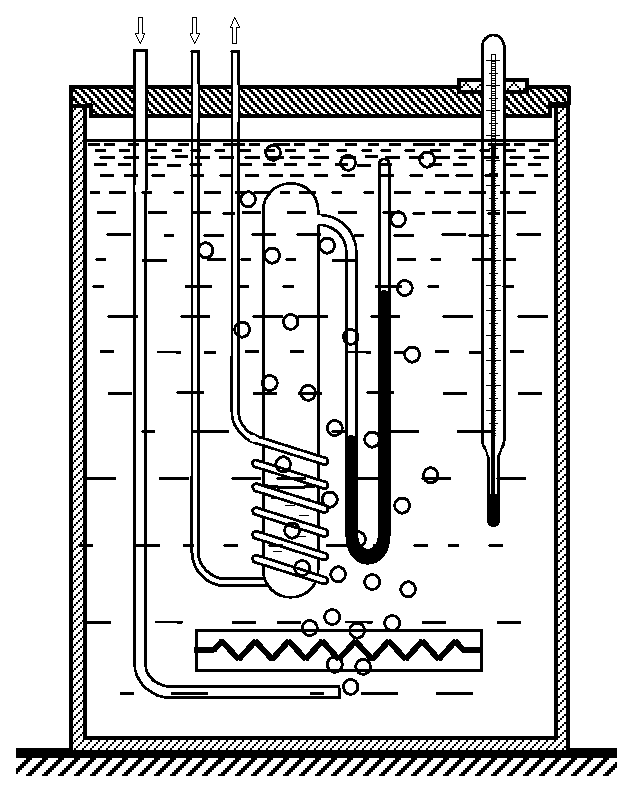
\includegraphics[width=\vva]{pic/O1}}%
%\hfil
%\hbox to \vvb{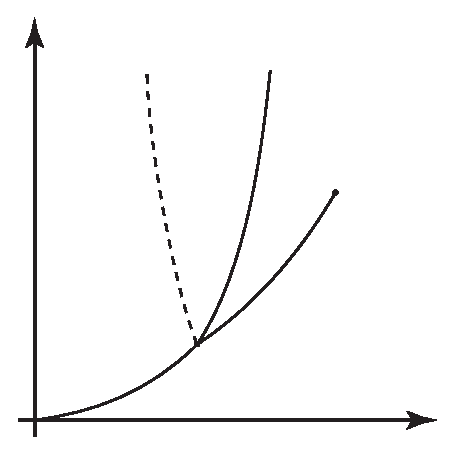
\includegraphics[width=\vvb]{pic/O2}}%

\vfill

\newpage

\setcounter{page}{1}
\thispagestyle{empty}\mbox{}
%\vskip5mm

\begingroup
\parindent=0pt\centering
{\scriptsize
Министерство науки и высшего образования Российской Федерации\\
Федеральное государственное автономное\\
образовательное учреждение высшего образования\\
<<Московский физико-технический институт\\ 
(национальный исследовательский университет)>>\par
}

\vskip 20mm

{\bfseries\LARGE\strut ЛАБОРАТОРНЫЙ\strut\\ ПРАКТИКУМ\strut\\ ПО ОБЩЕЙ ФИЗИКЕ\strut}

\vskip 10mm

{\bfseries\Large В трёх томах}

\vskip 10mm

{\bfseries\Large Том 2}

\vskip 5mm

{\bfseries\Large \MakeUppercase{\nazvan}}

\vskip 5mm

Издание второе, переработанное и дополненное

\vskip 20mm

%{\it\small Рекомендовано\\ Учебно-методическим объединением\\
%высших учебных заведений Российской Федерации\\
%по образованию в области прикладных математики и физики\\
%в качестве учебного пособия для студентов вузов\\
%по направлению подготовки <<Прикладные математика и физика>> }

\vskip 10mm

{\bfseries Под редакцией\strut\\
% проф. А.Д.~ГЛАДУНА\strut}
проф. А.\,В.~МАКСИМЫЧЕВА и проф. М.\,Г.~НИКУЛИНА\strut}

\vfill

{\small МОСКВА\\
МФТИ\\
\god}\par
\endgroup

\newpage

\setcounter{page}{2}

\thispagestyle{empty}

{\parindent=0pt {\footnotesize
УДК 53(075)\\
ББК 22.3я73\\
\phantom{УДК }Л12
}

{\centering\small
А в т о р ы:

М.\,Г.~Никулин,
П.\,В.~Попов,
Д.\,А.~Александров,
Н.\,С.~Берюлёва,
В.\,П.~Кириллов,
Г.\,Р.~Локшин,
А.\,А.~Нозик,
\ldots

%TODO Уточнить список авторов!

\vskip 5mm

{\small Р е ц е н з е н т ы:

Кафедра общей физики\\ Национального исследовательского
ядерного университета <<МИФИ>>\\
(зав. кафедрой доктор физико-математических наук,\\
профессор {\it Н.\,П. Калашников})

\smallskip

Зав. отделом оптики ФИАН\\ доктор физико-математических наук,
профессор  {\it А.\,В. Масалов}}

}}

\vskip 5mm

\newlength{\vvc}

\settowidth{\vva}{Л12} \setlength{\vvc}{\textwidth} \addtolength{\vvc}{-\vva} \setlength{\vvb}{1em}
\addtolength{\vvc}{-\vvb}

\noindent
\parbox[t]{\vva}{\mbox{}\\Л12}%
\hskip\vvb
\vva=\parindent
\parbox[t]{\vvc}{\parindent=\vva
{\bfseries Лабораторный практикум по общей физике}: учеб. пособие. В трёх
томах.
{\bfseries Т.~\tom. \nazvan}~/ Никулин М.\,Г.,
Попов П.\,В., Александров Д.\,А. и др.; под ред. А.\,В.~Максимычева.~---  
М.\,: МФТИ, \god. --- \pageref{all_page}~с.

ISBN 978-5-7417-0507-0

}

\vskip 5mm

{\small Представлены лабораторные работы по электричеству и магнетизму 
    для студентов II курса (3-го семестра) МФТИ. 
    Работы распределены по ключевым разделам курса общей физики.
Каждый раздел содержит теоретическое введение по рассматриваемому 
кругу физических явлений. Теоретические введения и описания составлены 
с таким расчётом, чтобы студент мог получить ясное представление о
лабораторной работе и изучаемом явлении и в том случае,
когда выполнение работы опережает теоретический курс.

Книга снабжена необходимым справочным материалом.

Для физических, инженерно-физических и физико-технических специальностей вузов.

Табл. ??.  Ил. ??.}

{\footnotesize
\hfill\parbox{2cm}{\bfseries УДК 53(075)\\
ББК 22.3я73\par}

\vskip 4mm

%TODO Уточнить ISBN

\settowidth{\vva}{\footnotesize\bf ISBN 978-5-7417-0507-0 (Т.\tom)}%
\noindent
\parbox[t]{\vva}{\footnotesize\bf
ISBN 978-5-7417-0507-0 (Т.\tom)\\
ISBN 978-5-7417-0200-7
}
\setlength{\vvc}{\textwidth}%
\addtolength{\vvc}{-\vva}%
\setlength{\vvb}{3em}%
\addtolength{\vvc}{-\vvb}%
\hfill
\copyright~\parbox[t]{\vvc}{%
\strut
М.\,Г.~Никулин,
П.\,В.~Попов,
Д.\,А.~Александров,
Н.\,С.~Берюлёва,
В.\,П.~Кириллов,
Г.\,Р.~Локшин,
А.\,А.~Нозик, \god}

\smallskip

\hfill
\copyright~\parbox[t]{\vvc}{\raggedright
Федеральное государственное автономное\\
образовательное учреждение\\
высшего профессионального образования\\
<<Московский физико-технический институт\\
(государственный университет)>>, \god}



}


\pagestyle{empty}
\tableofcontents
\pagestyle{main}

\cleardoublepage
\chapter{Измерения электрических и магнитных полей}

% Системы единиц. Урезать. Оставить только таблицы в конце
%\vn О системах единиц в классической электродинамике

При измерении физической величины $x$ её числовое значение \fs{x} свидетельствует о том, сколько раз в $x$ содержится
некоторая единица измерения \ks{x}. Это означает, что
\be1
\fs{x}=\frac{x}{\ks{x}}.
\ee
Если, например, сила тока $I=10$~А, то $\fs{I}=10$, $\ks{I}=1$~А. Соотношение (\r1) можно записать в виде
\be2
x=\fs{x}\ks{x}.
\ee
При уменьшении единицы измерения в $\alpha$ раз
\[
\ks{x}\rightarrow\ks{X}=\frac{1}{\alpha}\ks{x},\qquad\fs{x}\rightarrow\fs{X}=\alpha\fs{x}.
\]
Сама физическая величина при этом не изменяется, поскольку
\be3
x=\fs{x}\ks{x}=\fs{X}\ks{X}.
\ee

Для каждой физической величины можно в принципе установить свою единицу, никак не связанную с единицами других величин.
Это приводит, однако, к тому, что в уравнениях, выражающих физические законы, появляется множество численных
коэффициентов. Уравнения становятся необозримыми, формулы~--- слишком сложными. Чтобы избежать этого, в физике уже давно
отказались от независимого выбора единиц всех физических величин и стали применять системы единиц, построенные по
определённому принципу, который состоит в следующем. Некоторые величины принимаются за базисные, т.е. такие, для которых
единицы устанавливаются произвольно. Так, например, в механике применяется система ($L$, $M$, $T$), в которой за базисные
величины принимаются длина $L$, масса $M$ и время $T$. Выбор базисных величин и их число произвольны. Это вопрос
соглашения. В международной системе СИ в качестве базисных величин приняты девять величин: длина, масса, время, сила
электрического тока, температура, сила света, количество вещества, плоский угол, телесный угол. Величины, не являющиеся
базисными, называются производными. Для производных величин единицы устанавливаются на основе формул, служащих их
определением.

Здесь возникает понятие размерности. Если, например, число базисных величин равно трём и за них приняты длина $L$, масса
$M$ и время $T$, то для размерности производной величины $y$ имеем
\be4
\dim y=L^p\cdot M^q\cdot T^r,
\ee
где $p$, $q$, $r$~--- постоянные числа. Формула (\r4) показывает, что если единицы длины, массы и времени уменьшить в
$\alpha$, $\beta$ и $\gamma$ раз, то единица производной величины $y$ уменьшится в $\alpha^p\beta^q\gamma^r$ раз, и,
следовательно, её числовое значение увеличится в такое же число раз. В этом и состоит смысл понятия размерности.
Заметим, что для безразмерной величины~$z$
\[
\dim z=1.
\]
На практике величины $p$, $q$, $r$ оказываются рациональными числами. Это обусловлено соответствующими определениями
физических величин.

Часто размерность физической величины отождествляют с её единицей в соответствующей системе единиц. Так, например,
говорят, что скорость имеет размерность $м/с$, а давление $Н/м^2$. В этом нет большой беды, хотя, строго говоря, это
неверно: размерность скорости~--- $LT^{-1}$, а давления~--- $ML^{-1}T^{-2}$.

Рассмотрим вопрос о системах единиц в электродинамике. Законы макроскопической электродинамики определяются её
фундаментальными аксиомами~--- уравнениями Максвелла, которые являются концентрированным обобщением экспериментальных
фактов из области электричества и магнетизма. Запишем уравнения Максвелла для вакуума в произвольной системе единиц:

\def\urtab#1#2#3{%
\vskip-1ex
\be#3
\begin{array}{ll}
\hbox to 0.5\textwidth{$\ds #1$\hfil}&\hbox to 0.25\textwidth{$\ds #2$\hfil}
\end{array}
\ee
\vskip-1ex
}

\urtab{\oint_S \vec{E}d\vec{S}=\alpha\int_V\rho\,dV,}{\divv\vec{E}=\alpha\rho,}{5}

\urtab{\oint_S\vec{B}d\vec{S}=0,}{\divv\vec{B}=0,}{6}

\urtab{\oint_L\vec{E}d\vec{l}=-\beta\int_S\frac{\d{\vec{B}}}{\d t}\,d\vec{S},}{\rot\vec{E}=-\beta\frac{\d\vec B}{\d t},}{7}

\urtab{\oint_L\vec{B}d\vec{l}=\gamma\int_S\vec{j}\,d\vec{S}+\delta\int_S\frac{\d{\vec{E}}}{\d t}\,d\vec{S},}
{\rot\vec{B}=\gamma\vec{j}+\delta\frac{\d\vec E}{\d t};}{8}

\be9
\vec{F}=\xi q\vec{E}+\eta q\vec{v}\times\vec{B},
\ee
\be10
d\vec{F}=\xi dq\vec{E}+\eta Id\vec{l}\times\vec{B}.
\ee
Здесь приняты стандартные обозначения. Уравнение (\r9) или (\r{10}) служит для определения силовых векторов $\vec{E}$ и
$\vec{B}$. Множество коэффициентов ($\alpha$, $\beta$, $\gamma$, $\delta$, $\xi$, $\eta$) свидетельствует о том, что для
каждой физической величины, входящей в систему уравнений (\r5)~--~(\r{10}), принята собственная единица измерения,
независимая от единиц других величин.

Напомним физический смысл уравнений Максвелла. Уравнение (\r5) показывает, что источником электрического поля $\vec{E}$
является электрический заряд. Из него можно получить закон Кулона:
\be11
\vec{F}_{12}=\alpha\frac{q_1q_2}{4\pi r^3_{12}}\vec{r}_{12}.
\ee
Уравнение (\r6) говорит о том, что в природе отсутствуют, насколько известно в настоящее время, магнитные заряды.
Уравнение (\r7)~--- это математическая формулировка закона электромагнитной индукции. Оно свидетельствует о том, что
изменяющееся магнитное поле порождает вихревое электрическое поле. Уравнение (\r8) показывает, что магнитное поле
$\vec{B}$~--- всегда вихревое (силовые линии замкнуты), и его источником являются не только движущиеся заряды, но и
переменное электрическое поле. Для постоянного магнитного поля с помощью (\r8) можно получить закон Био--Савара (см.
Приложение):
\be12
d\vec{B}=\frac{\gamma}{4\pi}\frac{I\,d\vec{l}\times\vec{r}}{r^3}.
\ee

С помощью уравнения
\[
\oint\vec{B}\cdot d\vec{l}=\gamma\int\vec{j}\cdot\vec{S}
%\rot\vec{B}=\gamma\vec{j}
\]
можно найти отнесённую к единице длины силу взаимодействия между двумя токами $I_1$ и $I_2$, текущими по двум бесконечно
длинным параллельным проводам:
\be13
\frac{dF}{dl}=\gamma\eta\frac{I_1I_2}{2\pi r}.
\ee

Рассмотрим электромагнитное поле в области, где нет источников, т.е. $\rho=0$ и $\vec{j}=0$. В силу (\r7) и (\r8) имеем
\[
\rot\,\rot\vec{E}=-\beta\frac{\d}{\d t}\rot\vec{B}=-\beta\delta\frac{\d^2\vec{E}}{\d t^2}
\]
или
\[
\grad\,\divv\vec{E}-\nabla^2\vec{E}=-\beta\delta\frac{\d^2\vec{E}}{\d t^2},
\]
т.е.
\be14
\nabla^2\vec{E}=\beta\delta\frac{\d^2\vec{E}}{\d t^2}.
\ee
Волновое уравнение (\r{14}) описывает распространение электромагнитных волн в вакууме. Скорость распространения волн
равна ${1}/{\sqrt{\beta\delta}}$. Измерения дают ${1}/\sqrt{\beta\delta}=c$, где $c$~--- скорость света в вакууме. Таким
образом, из опыта следует, что $\beta\delta=1/c^2$, где $c$~--- универсальная фундаментальная постоянная.

Запишем уравнения (\r5)~--~(\r9) в безразмерном виде. Для каждой физической величины $f$, входящей в эту систему, введём
следующие обозначения:
\be15
\fs{f}\equiv f',\quad\ks{f}\equiv f_0,\quad\text{т.е.}\quad f'=\frac{f}{f_0}\quad или\quad f=f'\.f_0.
\ee
Для единиц длины $l$ и времени $\tau$ имеем
\be16
\vec{r}=\vec{r}\,'\cdot l,\qquad t=t'\cdot\tau.
\ee

Подставляя (\r{15}) и (\r{16}) в систему (\r5)~--~(\r9) и опуская штрихи, находим

\def\urtab#1#2#3{%
\vskip-1ex
\be#3
\begin{array}{ll}
\hbox to 0.5\textwidth{$\ds #1$\hfil}&\hbox to 0.3\textwidth{$\ds #2$\hfil}
\end{array}
\ee
\vskip-1ex
}

\urtab{E_0l^2\oint_S \vec{E}d\vec{S}=\alpha\rho_0l^3\int_V\rho\,dV,}
{\frac{E_0}{l}\divv \vec{E}=\alpha\rho_0\rho,}{17}

\urtab{\oint_S\vec{B}d\vec{S}=0,}{\divv\vec{B}=0,}{18}

\urtab{E_0l\oint_L\vec{E}d\vec{l}=-\beta\frac{B_0}{\tau}l^2\int_S\frac{\d{\vec{B}}}{\d t}\,d\vec{S},}
{\frac{E_0}{l}\rot\vec{E}=-\frac{\beta B_0}{\tau}\frac{\d\vec B}{\d t},}{19}

%B_0l\oint_L\vec{B}d\vec{l}=
%\gamma j_0l^2\int_S\vec{j}\,d\vec{S}+\delta\frac{E_0l^2}{\tau}\int_S\frac{\d{\vec{E}}}{\d t}\,d\vec{S}&
%\frac{B_0}{l}\rot\vec{B}=\gamma j_0\vec{j}+\frac{\delta E_0}{\tau}\frac{\d\vec E}{\d t},&\num{20}\\


\be20
\begin{array}{ll}
\hbox to 0.4\textwidth{$\ds B_0l\oint_L\vec{B}d\vec{l}=
\gamma j_0l^2\int_S\vec{j}\,d\vec{S}+\delta\frac{E_0l^2}{\tau}\int_S\frac{\d{\vec{E}}}{\d t}\,d\vec{S},$\hss}&\\ [4ex]
&\ds\frac{B_0}{l}\rot\vec{B}=\gamma j_0\vec{j}+\frac{\delta E_0}{\tau}\frac{\d\vec E}{\d t},
\end{array}
\ee

\iffalse
\be17
E_0l^2\oint_S \vec{E}d\vec{S}=\alpha\rho_0l^3\int_V\rho\,dV
\qquad\frac{E_0}{l}\divv \vec{E}=\alpha\rho_0\rho,
\ee
\be18
\oint_S \vec{B}d\vec{S}=0
\qquad\divv \vec{B}=0,
\ee
\be19
E_0l\oint_L\vec{E}d\vec{l}=-\beta\frac{B_0}{\tau}l^2\int_S\frac{\d{\vec{B}}}{\d t}\,d\vec{S}
\qquad\frac{E_0}{l}\rot\vec{E}=-\frac{\beta B_0}{\tau}\frac{\d\vec B}{\d t},
\ee
\be20
B_0l\oint_L\vec{B}d\vec{l}=\gamma j_0l^2\int_S\vec{j}\,d\vec{S}+\delta\frac{E_0l^2}{\tau}\frac{\d{\vec{E}}}{\d t}\,d\vec{S}
\qquad\frac{B_0}{l}\rot\vec{B}=\gamma j_0\vec{j}+\frac{\delta E_0}{\tau}\frac{\d\vec E}{\d t},
\ee

\fi

\be21
F_0\vec{F}=\xi q_0qE_0\vec{E}+\eta q_0qv_0B_0\vec{v}\times\vec{B}.
\ee
Здесь $\ds v_0=\frac{l}{\tau}$, $j_0=\rho_0v_0$.

Из (\r{17})~--~(\r{21}) следует, что
\[
\dim\alpha=\dim\frac{E_0}{\rho_0l},
\]
\[
\dim\beta=\dim\frac{1}{v_0}\frac{E_0}{B_0},
\]
\[
\dim\gamma=\dim\frac{B_0}{j_0l},
\]
\[
\dim\frac{\delta}{\gamma}=\dim\frac{j_0\tau}{E_0}=\dim\frac{\rho_0v_0\tau}{E_0}=\dim\frac{\rho_0l}{E_0},
\]
\[
\dim\delta=\dim\frac{1}{v_0}\frac{B_0}{E_0},
\]
\[
\dim\frac{\xi}{\eta}=\dim v_0\frac{B_0}{E_0}.
\]
Отсюда можно видеть, что
\[
\dim\frac{\alpha\delta}{\gamma}=1,\qquad \dim\frac{\xi\beta}{\eta}=1,
\]
\[
\dim\delta\beta=\dim\frac{1}{v_0^2}.
\]
Последнее соответствует тому, что
\[
\delta\beta=\frac{1}{c^2}.
\]
При выборе базисных единиц естественно предположить, что
\be22
\frac{\alpha\delta}{\gamma}=1,\quad\frac{\xi\beta}{\eta}=1,\quad \delta\beta=\frac{1}{c^2}.
\ee
В таблице \r{tab1} показано, как в различных системах пользуются произволом, который дают соотношения (\r{22}). В
настоящее время принято считать, что $c=299\,792\,458$~м/с (точно). Это означает, что базисные единицы <<привязаны>> к
этой величине. Это, конечно, соглашение. Мы полагаем в лаборатории $c\cong3\.10^8$~м/с.

В общей физике в настоящее время используются в основном две системы единиц: гауссова система СГС (далее~--- система СГС)
и международная система СИ (далее~--- система СИ). Система СГС, в которой в качестве базисных величин приняты длина,
масса и время, разработана на основе законов механики Ньютона. Электрические и магнитные величины вводятся в ней как
производные механических. Построенные по такому принципу системы единиц называются абсолютными. В системе СГС
электрические величины измеряются в единицах СГСЭ, а магнитные~--- в единицах СГСМ.

В системе СИ к трём базисным механическим величинам~--- длине, времени и массе~--- в электродинамике добавлена
независимая чисто электрическая величина, имеющая собственную размерность. В качестве таковой выбрана сила
электрического тока, а её единицей выбран ампер. Единицей заряда при этом является ампер-секунда, называемая кулоном.

\begin{table}[!t]
\tab{1}{Некоторые системы единиц, используемые при изучении макроскопической электродинамики}{%
\def\vph{\vphantom{$\ds\frac{A}{B}$}}\def\pp#1{\hbox to 5mm{\hfil #1\hfil}}%
\bt{|l|c|c|c|c|c|c|c|c|c|}\hline
\vph&\pp{$\alpha$}&\pp{$\beta$}&\pp{$\gamma$}&\pp{$\delta$}&\pp{$\xi$}&\pp{$\eta$}&\pp{$\frac{\alpha\delta}{\gamma}$}&
\pp{$\frac{\xi\beta}{\eta}$}&\pp{$\delta\beta$}\\ \hline
\vph СГСЭ&$4\pi$&1&$\frac{4\pi}{c^2}$&$\frac{1}{c^2}$&1&1&1&1&$\frac{1}{c^2}$\\ \hline
\vph СГСМ&$4\pi c^2$&1&$4\pi$&$\frac{1}{c^2}$&1&1&1&1&$\frac{1}{c^2}$\\ \hline
\vph СГС&$4\pi$&$\frac{1}{c}$&$\frac{4\pi}{c}$&$\frac{1}{c}$&1&$\frac{1}{c}$&1&1&$\frac{1}{c^2}$\\ \hline
\vph СИ&$\frac{1}{\e_0}$&1&$\frac{1}{\e_0c^2}$&$\frac{1}{c^2}$&1&1&1&1&$\frac{1}{c^2}$\\ \hline
\vph МКС&1&1&$\frac{1}{c^2}$&$\frac{1}{c^2}$&1&1&1&1&$\frac{1}{c^2}$\\ \hline
\multicolumn{10}{|l|}{\vph \hskip 1cm $c=299\,792\,458$~м/с (точно);}\\
\multicolumn{10}{|l|}{\vph\hskip 1cm $\e_0=8,854\.10^{-12}$~Ф/м;~~~$\mu_0=\frac{1}{\e_0c^2}=4\pi\.10^{-7}$~Гн/м.}\\ \hline
\et
}
\vskip-2em
\end{table}

Эталон силы электрического тока устанавливается на основе формулы (\r{13}). В системе СИ $\gamma=\frac{1}{\e_0c^2}$,
$\eta=1$, поэтому
\be23
\D F=\frac{1}{\e_0c^2}\frac{I_1I_2}{2\pi r}\D l.
\ee
На основании международного соглашения принято по определению, что ампер~--- это единица силы тока, который, проходя по
двум параллельным прямолинейным проводникам бесконечной длины и исчезающе малого кругового сечения, расположенным на
расстоянии 1~м друг от друга в вакууме, вызывал бы между проводниками силу, равную $2\.10^{-7}$~Н на каждый метр длины.
Реализовать эту единицу можно несколькими способами, например, измеряя силу взаимодействия двух катушек с постоянным
током.

Полагая в (\r{23}) $I_1=I_2=1$~А, имеем
\[
2\.10^{-7}~Н=\frac{1}{\e_0c^2}\frac{1}{2\pi}~Н,
\]
т.е.
\[
\frac{1}{\e_0c^2}=4\pi\.10^{-7}~\text{ед. СИ}
\]
или
\[
\e_0=\frac{10^{7}}{4\pi c^2}\approx 8,85\.10^{-12}~\text{ед. СИ.}
\]

В системе СГС единиц формула (\r{13}) имеет вид
\be24
\D F=\frac{4\pi}{c^2}\frac{I_1I_2}{2\pi r}\D l.
\ee

Установим соотношение между единицами силы электрического тока в системе СГС и системе СИ. Полагая в (\r{23})
$I_1=I_2=1$~А, $r=\D l=1$~м, находим
\be25
\D F=2\.10^{-7}~Н.
\ee
Воспользуемся теперь для вычисления той же силы формулой (\r{24}). Полагая в этой формуле $I_1=I_2=I$, $r=\D l=100$~см,
находим
\be26
\D F=\frac{4\pi}{c^2}\frac{I^2}{2\pi}=\frac{2I^2}{c^2}~дин=\frac{2I^2}{c^2}10^{-5}~Н.
\ee
Приравнивая (\r{25}) и (\r{26}), имеем
\[
2\.10^{-7}=\frac{2I^2}{c^2}10^{-5},\qquad т.е.\qquad I=3\.10^9~\text{ед. СГС}.
\]
Это означает, что
\be27
10\ks{I}_{СИ}=c\ks{I}_{СГС},
\ee
где $c=3\.10^{10}$~см/с, $\ks{I}_{СИ}=1$~А. Соотношение (\r{27}) можно представить в виде
\[
\ks{I}_{СИ}=3\.10^9\ks{I}_{СГС}
\]
или
\be28
c=10\frac{\fs{I}_{СГС}}{\fs{I}_{СИ}}\left(\frac{см}{с}\right),
\ee
что может быть проверено экспериментально (см. работу \textnumero~3.1.1).

В силу (\r{27}) для электрического заряда имеем
\[
\ks{q}_{СИ}=3\.10^9\ks{q}_{СГС}.
\]
Установим соотношение между единицами разности потенциалов в системе СГС и системе СИ. Воспользуемся для этого формулой
для отсчитываемого от бесконечно удалённой точки потенциала точечного заряда:
\[
\phi=\frac{q}{r}\quad (СГС),\qquad\qquad
\phi=\frac{1}{4\pi\e_0}\frac{q}{r}\quad (СИ).
\]
Пусть $q=1$~ед. СГС, а $r=1$~см, тогда $\phi=1~ед.~СГС\equiv\ks{\phi}_{СГС}$. Вычислим этот же потенциал в системе СИ:
\[
\phi=\frac{9\.10^9}{3\.10^9\cdot10^{-2}}=300~В.
\]
Это означает, что для единиц разности потенциалов имеем
\be29
\ks{U}_{СГС}=300\ks{U}_{СИ}.
\ee
Соотношение (\r{29}) может быть также проверено экспериментально, например, с помощью абсолютного вольтметра (см. работу
\textnumero~3.1.2).

Подобным образом устанавливаются соотношения между единицами других физических систем, величин (см. таблицу~\r{tab2}).
Основные формулы в системах СИ и СГС представлены в таблице~\r{tab3}.

\newpage

\tab{2}{Перевод числовых значений физических величин из~системы СИ в~систему СГС}{%
%\def\vs{\vphantom{$\ds\frac{A}{B}$}}%
\let\vs=\tabstrut
\def\bbx{\raggedright\baselineskip=9pt}%
\def\pbl#1#2{\parbox{#1}{\bbx #2}}%
\def\vr{\vbox to 3pt{}}%
\def\pb#1{$\vcenter{\vr\hbox{\pbl{30mm}{#1\hfill}}\vr}$}%
\bt{|l|c|c|c|}\hline
\vs Наименование&Обозн.&СИ&СГС\\ \hline
\vs Длина&$l$&1 м (метр)&$10^2$~см\\ \hline
\vs Масса&$m$&1 кг (килограмм)&$10^3$ г\\ \hline
\vs Время&$t$&1 с (секунда)&1 с\\ \hline
\vs Работа, энергия&$A$, $W$&1 Дж (джоуль)&$10^7$ эрг\\ \hline
\vs Мощность&$N$&1 Вт (ватт)&$10^7~\frac{эрг}{с\mathstrut}$\\ \hline
\vs Давление&$P$&1 Па (паскаль)&$10~\frac{дин}{см^2\mathstrut}$\\ \hline
\vs \pb{Сила электри-\\ческого тока}&$I$&1 А (ампер)&$3\.10^9$\\ \hline
\vs Электр. заряд&$q$&1 Кл (кулон)&$3\.10^9$\\ \hline
\vs Поляризация&$\vec{P}$&$1~\frac{Кл}{м^2}$&$3\.10^5$\\ \hline
\vs \pb{Электрическая индукция}&$\vec{D}$&$1~\frac{Кл}{м^2}$&$12\pi\.10^5$\\ \hline
\vs Электр. ёмкость&$C$&1 Ф (фарад)&$9\.10^{11}$ см\\ \hline
\vs \pb{Электрическое сопротивление}&$R$&1 Ом (ом)&$\frac{1}{9\.10^{11}}~\frac{с}{см\mathstrut}$\\ \hline
\vs \pb{Удельное сопротивление}&$\rho$&1 Ом\.м&$\frac{1}{9\.10^{9}\mathstrut}~с$\\ \hline
\vs \pb{Электрическая проводимость}&$\Lambda=\frac{1}{R}$&1 См (сименс)&$9\.10^{11}~\frac{см}{с\mathstrut}$\\ \hline
\vs \pb{Удельная проводимость}&$\sigma$&$1~\frac{См}{м}$&$9\.10^9~с^{-1}$\\ \hline
\vs Магнитный поток&$\Phi$&1 Вб (вебер)&$10^8$ Мкс\\ \hline
\vs \pb{Магнитная индукция}&$\vec{B}$&1 Тл (тесла)&$10^4$ Гс\\ \hline
\vs \pb{Напряжённость магнитного поля}&$\vec{H}$&$1~\frac{А}{м}$&$4\pi\cdot10^{-3}$ Э\\ \hline
\vs Намагниченность&$\vec{M}$&$1~\frac{А}{м}$&$\frac{1}{4\pi}\cdot 10^4$ Гс\\ \hline
\vs Индуктивность&$L$&1 Гн (генри)&$10^9$ см\\ \hline
\vs \pb{Электрический потенциал}&$\phi$&$1~В$ (вольт)&$\frac{1}{300}$\\ \hline
\vs \pb{Напряжённость электр. поля}&$\vec{E}$&$1~\frac{В}{м}$&$\frac{1}{3}\cdot 10^{-4}$\\ \hline
\et
}

\newpage

%\ftab{
\tab{3}{Основные формулы в СИ и СГС}{\small%
\let\vs=\tabstrut
\def\bbx{\raggedright\baselineskip=10pt}%
\def\pbl#1#2{\parbox{#1}{\bbx #2}}%
\def\vr{\vbox to 2pt{}}%
\def\pb#1{\vs$\vcenter{\vr\hbox{\pbl{38mm}{#1\hfill}}\vr}$}%
\bt{l|c|c}\hline
\vs Наименование&СИ&СГС\\ \hline
\pb{Уравнения Максвелла}&$\divv\vec{D}=\rho$&$\divv\vec{D}=4\pi\rho$\\
\pb{в дифференциальной}&$\divv\vec{B}=0$&$\divv\vec{B}=0$\\
\pb{форме}&$\rot\vec{E}=-\frac{\d\vec{B}}{\d t}$&$\rot\vec{E}=-\frac{1}{c}\frac{\d\vec{B}}{\d t}$\\
\pb{}&$\rot\vec{H}=\vec{j}+\frac{\d\vec{D}}{\d t}$&$\rot\vec{H}=\frac{4\pi}{c}\vec{j}+\frac{1}{c}\frac{\d\vec{D}}{\d t}$\\
\pb{Электрическая индукция}&$\vec{D}=\e_0\vec{E}+\vec{P}$&$\vec{D}=\vec{E}+4\pi\vec{P}$\\
\pb{Напряжённость магнитного поля}&$\vec{H}=\frac{1}{\mu_0}\vec{B}-\vec{M}$&$\vec{H}=\vec{B}-4\pi\vec{M}$\\
\\
\pb{Материальные}&$\vec{P}=\alpha\e_0\vec{E}$&$\vec{P}=\alpha\vec{E}$\\
\pb{уравнения}&$\vec{D}=\e\e_0\vec{E}$&$\vec{D}=\e\vec{E}$\\
%\pb{Связь между $\vec{D}$ и $\vec{E}$ в~вакууме}&$\vec{D}=\e_0\vec{E}$&$\vec{D}=\vec{E}$\\
&$\vec{M}=\kappa\vec{H}$&$\vec{M}=\kappa\vec{H}$\\
&$\vec{B}=\mu\mu_0\vec{H}$&$\vec{B}=\mu\vec{H}$\\
\pb{}&$\vec{j}=\sigma\vec{E}$&$\vec{j}=\sigma\vec{E}$\\
\\
%\pb{Связь между $\vec{B}$ и $\vec{H}$ в~вакууме}&$\vec{B}=\mu_0\vec{H}$&$\vec{B}=\vec{H}$\\
\pb{Уравнения Максвелла}&$\oint\limits_{S}\v{D}\,d\v{S}=\int_{V}\rho\,dV$&
$\oint\limits_{S}\v{D}\,d\v{S}=4\pi\int_{V}\rho\,dV$\\
\pb{в интегральной форме}&$\oint\limits_{S}\v{B}\,d\v{S}=0$&$\oint\limits_{S}\v{B}\,d\v{S}=0$\\
\pb{}&$\oint\limits_{L}\v{E}\,d\v{l}=-\int_{S}\frac{\d\vec{B}}{\d t}\,d\vec{S}$&
$\oint\limits_{L}\v{E}\,d\v{l}=-\frac{1}{c}\int_{S}\frac{\d\vec{B}}{\d t}\,d\vec{S}$\\
\pb{}&$\oint\limits_{L}\v{H}\,d\v{l}=$~~~~~~~~~~&$\oint\limits_{L}\v{H}\,d\v{l}=$~~~~~~~~~~\\
\pb{}&$=\int_{S}\vec{j}\,d\vec{S}+\int_{S}\frac{\d\vec{D}}{\d t}\,d\vec{S}$&
$=\frac{4\pi}{c}\int_{S}\vec{j}\,d\vec{S}+\frac{1}{c}\int_{S}\frac{\d\vec{D}}{\d t}\,d\vec{S}$\\
\pb{Сила Лоренца}&$\vec{F}=q\v{E}+\vp{\vec{v}}{\vec{B}}$&
$\ds\vec{F}=q\v{E}+\frac{q\mathstrut}{c\mathstrut}\vp{\vec{v}}{\vec{B}}$\\
\pb{Закон Кулона}&$\ds \v{F}=\frac{1}{4\pi\e_0}\frac{q_1q_2}{\e r^3}\v{r}$&$\ds\v{F}=\frac{q_1q_2}{\e r^3}\v{r}$\\[2ex]
\pb{Закон Био--Савара}&$\ds d\vec{H}=\frac{I}{4\pi}\frac{\vp{d\vec{l}}{\vec{r}}}{r^3}$&
$\ds d\vec{H}=\frac{I}{c}\frac{\vp{d\vec{l}}{\vec{r}}}{r^3}$\\[2ex]
\pb{Закон Ампера}&$d\vec{F}=I\vp{d\vec{l}}{\vec{B}}$&$d\vec{F}=\frac{I}{c}\vp{d\vec{l}}{\vec{B}}$\\
\pb{Плотность энергии электромагнитного поля}&$w=\frac12\bigl(\vec{E}\vec{D}+\vec{B}\vec{H}\bigr)$&
$w=\frac{1}{8\pi}\bigl(\vec{E}\vec{D}+\vec{B}\vec{H}\bigr)$\\
\pb{Вектор Пойнтинга}&$\vec{\Pi}=\vp{\vec{E}}{\vec{H}}$&$\ds\vec{\Pi}=\frac{c}{4\pi}\vp{\vec{E}}{\vec{H}}$\\[1ex]
\pb{Энергия магнитного поля тока}&$\ds W=\frac{LI^2}{2}$&$\ds W=\frac{1}{c^2}\frac{LI^2}{2}$\\[1ex]
\pb{Плотность импульса электромагнитного поля}&$\ds\vec{g}=\frac{1}{c^2}\vp{\vec{E}}{\vec{H}}$&
$\ds\vec{g}=\frac{1}{4\pi c}\vp{\vec{E}}{\vec{H}}$\\
\hline
\et
}
%}

\newpage

\conttab{\small%
\let\vs=\tabstrut
\def\bbx{\raggedright\baselineskip=10pt}%
\def\pbl#1#2{\parbox{#1}{\bbx #2}}%
\def\vr{\vbox to 3pt{}}%
\def\pb#1{\vs$\vcenter{\vr\hbox{\pbl{35mm}{#1\hfill}}\vr}$}%
\bt{l|c|c}\hline
\vs Наименование&СИ&СГС\\ \hline
\pb{Индуктивность (определение)}&$\Phi=LI$&$\ds\Phi=\frac{1}{c}LI$\\
\pb{Индуктивность длинного соленоида}&$\ds L=\frac{\mu\mu_0N^2S}{l}$&$\ds L=\frac{4\pi\mu N^2S}{l}$\\
\pb{Магнитный момент витка с током}&$\vec{\Mgot}=I\vec{S}$&$\ds\vec{\Mgot}=\frac{1}{c}I\vec{S}$\\
\pb{Момент сил, действующий на виток с~током}&$\vec{M}=\vp{\vec{\Mgot}}{\vec{B}}$&$\vec{M}=\vp{\vec{\Mgot}}{\vec{B}}$\\
\pb{Поле точечного магнитного диполя}&
$\vec{B}=\frac{\mu_0}{4\pi}\left(\frac{3(\vec{\Mgot}\vec{r})}{r^5}\vec{r}-\frac{\vec{\Mgot}}{r^3}\right)$
&$\vec{B}=\frac{3(\vec{\Mgot}\vec{r})}{r^5}\vec{r}-\frac{\vec{\Mgot}}{r^3}$\\
\pb{Сила, действующая на магнитный диполь в неоднородном поле}&$\vec{F}=(\vec{\Mgot}\vec{\nabla})\vec{B}$&
$\vec{F}=(\vec{\Mgot}\vec{\nabla})\vec{B}$\\
\pb{Поле точечного электрического диполя}&
$\vec{E}=\frac{1}{4\pi\e_0}\left(\frac{3(\vec{p}\vec{r})}{r^5}\vec{r}-\frac{\vec{p}}{r^3}\right)$&
$\vec{E}=\frac{3(\vec{p}\vec{r})}{r^5}\vec{r}-\frac{\vec{p}}{r^3}$\\
\pb{Ёмкость плоского конденсатора}&$\ds C=\frac{\e\e_0S}{d}$&$\ds C=\frac{\e S}{4\pi d}$\\
\pb{Энергия заряженного конденсатора}&$W=\frac{q^2}{2C}=\frac{qU}{2}=\frac{CU^2}{2}$&
$W=\frac{q^2}{2C}=\frac{qU}{2}=\frac{CU^2}{2}$\\ \hline
\et
}

Международная система СИ хорошо приспособлена для практических инженерных измерений. Она мало отличается от
электротехнической системы, предложенной Джорджи в начале ХХ~века (см. Приложение). В то время уравнения Максвелла мало
использовались в электротехнике, преобладали механические воззрения на природу электромагнитного поля. С точки зрения
рассмотренной выше структуры безразмерных параметров уравнений Максвелла выбор единиц системы СИ представляется
совершенно случайным, хотя вполне допустимым. С~теоретической точки зрения предпочтительной является система МКС, для
которой все коэффициенты равны единице, кроме коэффициентов $\gamma$ и  $\delta$, каждый из которых равен $1/c^2$ (см.
таблицу~\r{tab1}).
%Это обусловлено тем, что единственной электродинамической постоянной вакуума является скорость света $c$.

{\small

\lit

\n \emph{Камке Д., Кремер К.} Физические основы единиц измерения.~--- М.: Мир, 1980.

\n \emph{Власов А.Д., Мурин Б.П.}~Единицы физических величин в науке и технике. Справочник.~--- М.: Энергоатомиздат,
1990.

}


\introsection{Единицы измерения в электродинамике}
\label{sec:app_units}

При изучении нового класса физических явлений перед исследователем
неизбежно встаёт проблема выбора единиц измерения и эталонов новых
физических величин.

Проводя измерения, исследователь в первую очередь пользуется некоторым
базовым набором эталонов (например, секунда, метр и килограмм), и
в идеале новые единицы измерения должны определяться через базовые.
Однако пока законы, описывающие новое явление, остаются не понятыми,
выбор новых единиц измерения происходит по большому счету \emph{произвольно}.
Когда связь между <<новыми>> и <<старыми>>
явлениями устанавливается прочно, эти искусственно введённые эталоны
становятся избыточными, поскольку могут быть сведены к базовым. Однако,
поскольку главным условием выбора единиц служит, как правило,
их \emph{практическое удобство} и непосредственная
\emph{привязка к методикам измерения}~--- они часто остаются в употреблении,
а порой заносятся и в международные стандарты.

Например, на заре исследования тепловых явлений было создано множество
температурных шкал. Лишь позднее, когда была установлена связь температуры
с энергией идеального газа, все эти шкалы оказались, по сути, избыточны:
в качестве единиц измерения температуры можно использовать единицы
измерения энергии (например, джоули). Тем не менее по историческим
причинам в международную систему СИ вошла <<независимая>>
единица измерения температуры~--- \emph{кельвин}. Из-за этого во
всех термодинамических формулах приходится иметь дело с <<лишней>>
переводной константой~--- \emph{постоянной Больцмана}:
\[
k_{\text{Б}}\approx 1{,}38\cdot10^{-23}\;\text{Дж}/\text{К}.
\]

Аналогичная ситуация имела место и при исследовании электричества
и магнетизма. Более того, пока не было установлено единство электромагнитных
явлений, в каждой из этих областей была внедрена своя независимая
система единиц. Последующие попытки переработать и оптимизировать
систему электромагнитных единиц, чтобы избавить её от нефизичных
констант, имели весьма ограниченный успех, поскольку явление быстро
нашло широкое практическое применение и поменять что-либо радикально
было уже невозможно. В~результате в качестве международного стандарта
была принята система (СИ), содержащая <<лишнюю>>
базовую единицу~--- \emph{ампер}. При этом в теоретических работах,
не привязанных непосредственно к технике, сохранилась в употреблении
гауссова система (СГС), не содержащая избыточных эталонов (такие системы
единиц называют \emph{абсолютными}). При это возникает весьма неприятная
особенность: в разных системах различными оказываются не только 
\emph{единицы измерения} (как в механике), но и \emph{формулы}, их связывающие.

Практическая направленность этой книги вынуждает и нас придерживаться
в основном системы СИ (все лабораторные приборы проградуированы именно в СИ).
По умолчанию все формулы даны в системе СИ, если не указано иное. 
В работах данного раздела системы СИ и СГС используются совместно. 
В~разделе~V, посвящённом физике плазмы, используется традиционная для 
этой области система единиц СГС.

\introsubsection{Абсолютная (гауссова) система единиц}

Построим абсолютную систему единиц электродинамики, базирующуюся исключительно
на механических эталонах. За основу примем два твёрдо установленных
закона: Кулона и Ампера.

По сравнению с механикой, существенно новым понятием является \term{электрический
заряд}. Согласно закону Кулона, сила взаимодействия двух одинаковых
точечных зарядов пропорциональна квадрату заряда~$q$ и обратно пропорциональна
квадрату расстояния~$r$ между ними:
\begin{equation}
F_{\text{К}}=k_{q}\cdot\frac{q^{2}}{4\pi r^{2}},\label{eq:coulomb}
\end{equation}
где $k_{q}$~--- некоторая константа. Коэффициент $4\pi$ в знаменателе
поставлен из эстетических соображений,
чтобы подчеркнуть, что зависимость $\propto1/r^{2}$ в законе Кулона
(и в законе всемирного тяготения) возникает как площадь сферы в трёхмерном
пространстве.

На закон (\ref{eq:coulomb}) можно смотреть как на \emph{определение}
того, что такое электрический заряд.

Константа $k_{q}$ может быть выбрана \emph{произвольным} образом.
При этом, если мы не хотим вводить никаких дополнительных единиц измерения,
она должна быть \emph{безразмерна}. В гауссовой системе
полагают $k_{q}=4\pi$. Неплох также вариант $k_{q}=1$, сохраняющий
<<сферичность>> закона Кулона. Он предлагался в своё время
Лоренцем и другими известными физиками, но не прижился.

Тогда (\ref{eq:coulomb}) позволяет ввести единицу заряда с размерностью
\[
\left[q\right]=[F^{1/2}r]=\frac{M^{1/2}L^{3/2}}{T}.
\]
Здесь $\left(M,L,T\right)$~--- размерности базовых единиц массы,
длины и времени соответственно. По историческим причинам наибольшее
распространение получила абсолютная система с единицами \emph{сантиметр--грамм--секунда}
(СГС). Тогда единицу заряда можно определить как
\[
1~\text{ед. СГС заряда}=\frac{\text{г}^{1/2}\cdot\text{см}^{3/2}}{\text{с}}.
\]

Закон Ампера говорит о силовом взаимодействии \emph{токов}~--- то
есть \emph{движущихся} зарядов. Его можно сформулировать следующим
образом: сила взаимодействия двух параллельных проводников на единицу их длины
пропорциональна квадрату заряда, проходящему через них в единицу времени
(т.\,е. току $I=q/t$), и обратно пропорциональна расстоянию между ними:
\begin{equation}
\frac{F_{\text{А}}}{l}=k_{I}\frac{I^{2}}{2\pi r}\label{eq:ampere}
\end{equation}
($2\pi r$ --- длина окружности радиуса~$r$ вокруг провода).

Здесь уже все входящие в формулу величины вполне определены,
поэтому константа $k_{I}$ не может быть произвольной~--- её значение
должно быть получено \emph{из опыта}. Найдём её размерность:
\[
\left[k_{I}\right]=\left[\frac{F}{q^{2}}t^{2}\right]=\frac{T^{2}}{L^{2}}.
\]
То есть $k_{I}$ есть величина, обратная квадрату некоторой скорости.
Положим
\begin{equation}
k_{I}=\frac{k_{q}}{c^{2}},\label{eq:kikq}
\end{equation}
где $c$~--- константа, которую можно назвать \term{электродинамической
постоянной}, так как она связывает взаимодействия неподвижных и движущихся
зарядов. Отметим, что соотношение \ref{eq:kikq} должно выполняться
для всех систем измерения.

Как мы знаем сегодня, электродинамическая постоянная,
равная $c\approx3\cdot10^{10}\;\text{см}/\text{с}$,~--- не что иное
как \term{скорость света}, то есть максимальная скорость
распространения всех известных науке взаимодействий. В~настоящее время
эта константа относится к числу \emph{фундаментальных} и ей приписывают
\emph{точное} значение $c\equiv299\,792\,458\;\text{м/с}$
и используют для определения эталона метра через эталон секунды.

Таким образом, выбранные нами в качестве базовых законы Кулона и Ампера
выглядят как
\begin{equation}
F_{\text{К}}=\frac{q_{1}q_{2}}{r^{2}},\qquad F_{\text{А}}=\frac{2I_{1}I_{2}}{rc^{2}}l.\label{eq:col-amp}
\end{equation}

Теперь можно определить и остальные электродинамические величины.

\term{Напряжённость электрического поля} определяют (во всех системах)
как отношение силы Кулона к заряду:
\[
E=\frac{F}{q},\qquad\left[E\right]=\frac{M^{1/2}}{L^{1/2}T}=\frac{\text{г}^{1/2}}{\text{см}^{1/2}\cdot\text{с}}.
\]

\term{Индукцию магнитного поля} можно определить как отношение силы
на единицу длины провода к току в нём:
\begin{equation}
B=k_{B}\cdot\frac{F_{\text{А}}/l}{I}.\label{eq:kB}
\end{equation}
Выбор коэффициента $k_{B}$ опять-таки за нами. Зная о единстве электрического
и магнитного полей, его стоит выбрать таким, чтобы их размерности
\emph{совпадали}:
\[
\left[B\right]=\left[k_{B}\right]\cdot\left[\frac{F}{Il}\right]=\left[k_{B}\right]\cdot\frac{T}{L}\left[E\right].
\]
Видно что $k_{B}$ в таком случае должен иметь размерность скорости:
$\left[k_{B}\right]=L/T$, поэтому уместно положить $k_{B}=c$. Тогда
формулу для силы Ампера в терминах $B$ можно записать как
\begin{equation}
F_{\text{А}}=\frac{1}{c}IBl.
\end{equation}
Закон Ампера (\ref{eq:col-amp}) получится, если поле прямого провода
вычисляется как
\[
B_{\text{пр}}=\dfrac{2I}{cr}.
\]

Итак, на основе законов Кулона и Ампера мы определили единицы измерения
всех основных электродинамических величин: электрического заряда,
электрического и магнитного полей. Кроме того, \emph{теория размерностей}
позволила нам попутно установить существование фундаментальной константы~---
электродинамической постоянной~$c$.

\introsubsection{Система СИ}

Абсолютная система, предложенная выше, не могла быть разработана во
времена Ампера и Кулона, когда еще не было осознано единство электрических
и магнитных явлений.
% (исследования Ампера были \emph{первым} шагом
%в этом направлении).

Следуя системе СИ, выберем закон Ампера в качестве определения того,
что такое \term{электрический ток}. Помимо базовых единиц (\emph{метр--килограмм--секунда}),
СИ определяет \emph{независимый} эталон тока: при токе в 1~\emph{ампер} два
тонких провода на расстоянии 1~м взаимодействуют с силой $2\cdot10^{-7}$~Н
на 1~м их длины. Это значит, что константа $k_{I}$ в законе (\ref{eq:ampere}),
которую называют \term{магнитной постоянной} и традиционно обозначают
как~$\mu_{0}$, выбрана равной
\[
\mu_{0}=4\pi\cdot10^{-7}\;\text{Н}/\text{А}^{2}.
\]
Закон Ампера в этих единицах:
\begin{equation}
F_{\text{А}}=\mu_{0}\frac{I_{1}I_{2}}{2\pi r}l.
\end{equation}

Последствием введения лишнего эталона будет то, что во все <<магнитные>> формулы
войдёт дополнительная \emph{размерная константа} $\mu_0$, заданная \emph{точно}.
Она не имеет явного физического смысла, а её единственная функция~---
перевод между единицами измерения. Зато <<ампер>>~--- очень удобная
единица измерения тока: в частности, характерные значения токов в
большинстве бытовых электроприборов варьируются в пределах $10^{-2}\div10^2\;\text{А}$.

Имея эталон тока, можно определить единицу измерения заряда~--- \emph{кулон},
$1\;\text{Кл}=1\;\text{А}\cdot\text{с}$. При таком подходе константа~$k_{q}$ в законе Кулона (\ref{eq:coulomb}) может быть определена
из опыта. Как мы уже обсуждали выше, опыт даёт результат (\ref{eq:kikq}),
поэтому $k_{q}=\mu_{0}c^{2}$. Традиционно вводят обозначение
\begin{equation}
\varepsilon_{0}=\frac{1}{\mu_{0}c^{2}}\approx8{,}85\cdot10^{-12}\;\frac{\text{Кл}^{2}}{\text{Н}\cdot\text{м}^{2}}.
\end{equation}
Величину $\varepsilon_{0}$ называют \term{электрической постоянной}.
Она также является просто переводной константой, не имеющей
явного физического смысла. Физический смысл имеет электродинамическая
постоянная (она же скорость
света в вакууме):
\[
c = \frac{1}{\sqrt{\varepsilon_{0}\mu_{0}}}.
\]
%\begin{lab:note}
%Исторически использовались термины <<диэлектрическая
%проницаемость вакуума>> и <<магнитная проницаемость
%вакуума>>, которые ещё можно встретить в старых учебниках.
%Эти термины достались нам в наследство от теории эфира:
%вакуум считался заполненным некоторой упругой средой. По современным
%представлениям, отвергающим примитивную концепцию эфира, говорить
%о проницаемости вакуума бессмысленно.
%\end{lab:note}


Таким образом, закон Кулона в системе СИ имеет вид
\begin{equation}
F_{\text{К}}=\frac{1}{\varepsilon_{0}}\frac{q_{1}q_{2}}{4\pi r^{2}}.
\end{equation}

Наконец, константа $k_{B}$ в определении индукции магнитного поля
(\ref{eq:kB}) принимается равной единице. Поэтому справедлива формула
\begin{equation}
F_{\text{А}}=IBl.
\end{equation}
Поле прямого провода вычисляется как
\[
B_{\text{пр}}=\mu_{0}\dfrac{I}{2\pi r}.
\]

Наконец, выразим единицы измерения полей:
\[
\left[E\right]=\frac{\text{Н}}{\text{Кл}}=\frac{\text{В}}{\text{м}}=\frac{\text{кг}\cdot\text{м}}{\text{А}\cdot\text{с}^{3}}.
\]
Здесь $1\;\text{В}=1\;\text{Дж}/1\;\text{Кл}$ --- единица напряжения
\emph{вольт}. Единица индукции магнитного поля \emph{тесла}:
\[
\left[B\right]\equiv\text{Тл}=\frac{\text{Н}}{\text{А}^{2}}\cdot\frac{\text{А}}{\text{м}}=\frac{\text{кг}}{\text{А}\cdot\text{с}^{2}}.
\]
Видно, что размерности $E$ и $B$ в системе СИ разные. Их отношение имеет размерность
скорости: $\left[E/B\right]=\text{м/c}$.

\begin{lab:note}
Согласно решению международной комиссии по стандартам с 2019 года
планируется принять новые определения базовых единиц СИ, в том числе и ампера.
Его величина будет устанавливаться фиксацией численного значения
\emph{элементарного электрического заряда}, которое
планируется принять равным
\[
e = 1,602\,176\,634\cdot 10^{-19}\;\text{А}\cdot\text{с}\;(точно).
\]
При таком определении электрическая постоянная~$\varepsilon_0$ и, следовательно,
магнитная постоянная~$\mu_0$ приобретут погрешность и 
станут \emph{измеряемыми} величинами.
\end{lab:note}

\introsubsection[Уравнения электродинамики в произвольной системе 
единиц]{Уравнения электродинамики в произвольной системе 
единиц\protect\footnote{Если читатель ещё не знаком с системой 
    уравнений Максвелла, этот параграф можно пропустить.}}

Основными уравнениями электродинамики являются уравнения Максвелла
для электромагнитного поля, а также выражение для силы Лоренца, связывающее
эту теорию с механикой. Запишем эти уравнения для вакуума в произвольной
системе единиц (ограничимся дифференциальной формой):
\begin{align}
\Div \vec{E} & =k_{q}\rho,\label{eq:gauss}\\
\Div \vec{B} & =0,\\
\Rot \vec{E} & =-\frac{1}{k_{B}}\frac{\partial\vec{B}}{\partial t},\label{eq:faradey}\\
\frac{1}{k_B}\Rot \vec{B} & =k_{I}\left(\vec{j}+\frac{1}{k_{q}}\frac{\partial\vec{E}}{\partial t}\right);\label{eq:ampere-dif}
\end{align}
% \begin{comment}
% \begin{align*}
% \oint_{S}\vec{E}\cdot d\vec{S} & =k_{q}q, & \mathop{\mathrm{div}\vec{E}} & =k_{q}\rho,\\
% \oint_{S}\vec{B}\cdot d\vec{S} & =0, & \mathop{\mathrm{div}\vec{B}} & =0,\\
% \oint_{\Gamma}\vec{E}\cdot d\vec{l} & =-\frac{\partial}{\partial t}\int_{S}\frac{\vec{B}}{k_{B}}\cdot d\vec{S}, & \mathop{\mathrm{rot}}\vec{E} & =-\frac{1}{k_{B}}\frac{\partial\vec{B}}{\partial t},\\
% \oint_{\Gamma}\frac{\vec{B}}{k_{B}}\cdot d\vec{l} & =k_{I}\left(I+\frac{\partial}{\partial t}\int_{S}\frac{\vec{E}}{k_{q}}\cdot d\vec{S}\right), & \mathop{\mathrm{rot}}\vec{B} & =k_{B}k_{I}\left(\vec{j}+\frac{1}{k_{q}}\frac{\partial\vec{E}}{\partial t}\right).
% \end{align*}
% \end{comment}
\begin{equation}
\vec{F}_Л=q\left(\vec{E}+\frac{1}{k_{B}}\vec{v}\times\vec{B}\right).\label{eq:lorentz}
\end{equation}

Поясним кратко, почему коэффициенты будут именно такими.

В уравнении (\ref{eq:gauss}) (\emph{теорема Гаусса}) стоит коэффициент $k_q$,
поскольку из него непосредственно следует закон Кулона $E=k_{q}\frac{q}{r^{2}}$.

Одинаковые коэффициенты $1/k_{B}$ в уравнениях (\ref{eq:faradey})
(\emph{закон электромагнитной индукции Фарадея}) и (\ref{eq:lorentz})
(\emph{сила Лоренца}) отражают известную связь этих явлений
(см. [1, \S 64]).

В постоянном поле ($\partial/\partial t=0$) уравнение (\ref{eq:ampere-dif})
представляет собой \emph{теорему о циркуляции магнитного поля}. Из
неё, в частности, может быть выведен \emph{закон Био--Савара}
 (см. [2, \S 3.3]):
\[
\vec{B}=k_{B}k_{I}\oint\frac{\vec{j}\times\vec{r}dV}{4\pi r^{3}}=k_{B}k_{I}\oint\frac{Id\vec{l}\times\vec{r}}{4\pi r^{3}}.
\]
Поле прямого провода равно $B=k_{B}k_{I}\frac{I}{2\pi r}$, что в
совокупности с (\ref{eq:lorentz}) даёт закон Ампера для двух параллельных
токов:
\[
F_{\text{А}}=\frac{1}{k_{B}}I_{1}B_{2}l=k_{I}\frac{2I_{1}I_{2}}{4\pi r}l.
\]

Наконец, второе слагаемое в правой части (\ref{eq:ampere-dif}) (\emph{ток
смещения}) вводится в теорию для того, чтобы выполнялся
\emph{закон сохранения заряда}. Если взять дивергенцию от (\ref{eq:ampere-dif}),
должно получиться \emph{уравнение непрерывности}:
\[
\frac{\partial\rho}{\partial t}+\mathop{\mathrm{div}}\vec{j}=0
\]
(так как $\mathop{\mathrm{div}}\mathop{\mathrm{rot}}\vec{B}\equiv 0$),
что с учётом (\ref{eq:gauss}) и объясняет выбор множителя~$1/k_{q}$
перед плотностью тока смещения $\partial{\vec E}/\partial{t}$.

Если заряды и токи в системе отсутствуют, то система уравнений Максвелла
переходит, как известно, в \emph{волновое уравнение} для электрического
и магнитного полей. В частности,
\[
\frac{\partial^{2}E}{\partial t^{2}}=\frac{k_{q}}{k_{I}}\nabla^{2}\vec{E}.
\]
В вакууме электромагнитные волны распространяются со скоростью $c$,
поэтому, как уже говорилось выше, в любой системе единиц должно выполняться
соотношение (\ref{eq:kikq}): $k_{q}/k_{I}=c^{2}$.

В таблице~\tabref{coeffs} перечислены возможные комбинации коэффициентов $k_{q}$, $k_{I}=k_{q}/c^{2}$
и $k_{B}$ для наиболее часто встречающихся систем единиц измерения
(также приведены коэффициенты перед током в правой части (\ref{eq:ampere-dif})
$k_{B}k_{I}$ и перед током смещения $k_{B}k_{I}/k_{q}$).
Помимо рассмотренных выше СИ и СГС, здесь для справки представлены системы:
\begin{itemize}
\item СГСЭ --- система c эталонами \emph{сантиметр--грамм--секунда},
    в которой закон Кулона и сила Лоренца не содержат дополнительных постоянных:
    $F_К = q_1q_2/r^2$, $F_Л = q(\vec{E} + \vec{v}\times \vec{B})$.
\item СГСМ --- система c эталонами \emph{сантиметр--грамм--секунда},
в которой закон Ампера и сила Лоренца не содержат дополнительных постоянных:
$F_А = I_1I_2/r^2$, $F_Л = q(\vec{E} + \vec{v}\times \vec{B})$.
\item рационализированная МКС --- предложенная в начале XX в. Лоренцем система
с эталонами \emph{метр--килограмм--секунда}, в которой уравнения
Максвелла содержат единственную константу~--- скорость света~$c$.
\end{itemize}
Эти системы на сегодня практически полностью вытеснены системами~СИ и
СГС, причём использование последней ограничено в основном
теоретической физикой.

\begin{table}[h!]
    \caption{Коэффициенты в различных системах единиц}
    \small
    \renewcommand{\arraystretch}{2}
    \centering
    \begin{tabular}{cccccc}
        \toprule
        & $k_{q}$ & $k_{I}$ & $k_{B}$ & $k_{B}k_{I}$
        & $\dfrac{k_{B}k_{I}}{k_{q}}$\\
        \midrule
        СИ & $\dfrac{1}{\varepsilon_{0}}$ & $\mu_{0}$ & 1 & $\mu_{0}$
        & $\varepsilon_{0}\mu_{0}$\\[1ex] \hline
        СГС (гауссова) & $4\pi$ & $\dfrac{4\pi}{c^{2}}$ & $c$ & $\dfrac{4\pi}{c}$ & $\dfrac{1}{c}$ \\[1ex] \hline
        СГСЭ & $4\pi$ & $\dfrac{4\pi}{c^{2}}$ & 1 & $\dfrac{4\pi}{c^{2}}$
        & $\dfrac{1}{c^{2}}$ \\[1ex] \hline
        СГСМ & $4\pi c^{2}$ & $4\pi$ & 1 & $4\pi$ & $\dfrac{1}{c^{2}}$ \\[1ex] \hline
        МКС (рационализированная) & 1 & $\dfrac{1}{c^{2}}$ & $c$ & $\dfrac{1}{c}$ & $\dfrac{1}{c}$\\
        \bottomrule
    \end{tabular}
    \tabmark{coeffs}
\end{table}

\introsubsection{Перевод между системами единиц}

Установим связи между наиболее часто употребляемыми единицами в системах
СИ и гауссовой СГС. Прежде напомним соответствия между
важнейшими механическими единицами:
\[
1\,\text{Н}=10^{5}\,\frac{\text{г}\cdot\text{см}}{\text{с}^{2}}\equiv10^{5}\,\text{дин},\qquad1\,\text{Дж}=10^{7}\,\text{дин}\cdot\text{см}\equiv10^{7}\,\text{эрг}.
\]


\paragraph{Сила тока}

По определению, провод\'{а} с током $I=1\;\text{А}$ на расстоянии
$r=1\,\text{м}$ взаимодействуют с силой $F/l=2\cdot10^{-7}\,\frac{\text{Н}}{\text{м}}$.
Пользуясь формулой (\ref{eq:col-amp}), находим соответствующий ток
в единицах СГС:
\[
I=c\sqrt{\frac{F}{2l}r}=3\cdot10^{8}\frac{\text{м}}{\text{с}}\cdot\sqrt{10^{-7}\text{Н}}=3\cdot10^{10}\frac{\text{см}}{\text{с}}\cdot\sqrt{10^{-2}\text{дин}}=3\cdot10^{9}\;\text{ед. СГС}.
\]
Таким образом,
\[
1\;\text{А}=3\cdot10^{9}\;\text{ед. СГС},\qquad\text{или}\qquad1\;\text{ед. СГС}=\frac{1}{3}10^{-9}\;\text{А}.
\]

Все единицы измерения абсолютной системы могут быть выражены через
базовые (сантиметр, грамм, секунда). В частности, для тока
\[
1\;\text{ед. СГС тока}=\small\frac{\text{г}^{1/2}\cdot\text{см}^{3/2}}{\text{с}^{2}}.
\]
Видно, что базовые размерности СГС не очень эстетичны, поэтому, как правило,
пишут просто: <<ед. СГС>>. Иногда для единицы тока используется
название \emph{статампер} (статА, statA).

\paragraph{Заряд}

Поскольку заряд в обеих системах определяется по одной и той же формуле
$dq=Idt$, имеем очевидную связь:
\[
1\;\text{Кл}=3\cdot10^{9}\;\text{ед. СГС},\qquad\text{или}\qquad1\;\text{ед. СГС}=\frac{1}{3}10^{-9}\;\text{Кл}.
\]
Элементарный заряд (заряд электрона):
\[
e\approx1{,}6\cdot10^{-19}\;\text{Кл}=4{,}8\cdot10^{-10}\;\text{ед. СГС}.
\]

В иностранной литературе для абсолютной единицы заряда используется
название \emph{франклин}~(Фр, Fr) или \emph{статкулон} (statC).

\paragraph{Потенциал}

В системе СИ разность потенциалов (напряжение)
между точками равно $U[\text{СИ}]=1\,\text{В}$,
если работа $A=qU$ по перемещению заряда 1~Кл равна 1~Дж. Поэтому
\[
1\,\text{В}=1\;\frac{\text{Дж}}{\text{Кл}}=\frac{1}{300}\;\text{ед. СГС},\qquad1\,\text{ед. СГС}=300\,\text{В}.
\]
Абсолютную единицу напряжения называют иногда \emph{статвольт} (статВ, statV).


\paragraph{Магнитное поле}

Единицы измерения магнитных полей (магнитной индукции $B$) в СИ и СГС называются соответственно
\emph{тесла} (Тл) и \emph{гаусс}~(Гс).

Для их связи воспользуемся
законом Ампера: в СИ $F=IBl$, и в СГС $F=\frac{1}{c}IBl$. Тогда,
полагая $l=1\;\text{м}$, $I=1\;\text{А}$, $F=1\;\text{Н}$ и, соответственно,
$B=1\;\text{Тл}=1\;\frac{\text{Н}}{\text{А}\cdot\text{м}}$, находим
\[
B=\frac{cF}{Il}=\frac{3\cdot10^{10}\cdot10^{5}}{3\cdot10^{9}\cdot10^{2}}=10^{4}\;\text{ед. СГС}\cdot
\]
Таким образом,
\[
1\;\text{Тл}=10^{4}\;\text{Гс}.
\]

\emph{Напряжённость} магнитного поля~$H$ в вакууме выражается как $H=B/\mu_0$ 
(ед. СИ) и $H=B$ (ед. СГС). Для единиц измерения в СИ имеем: 
$[H] = \frac{Тл}{Н/А^2}=\frac{А}{м}$. В СГС единицы измерения напряжённости
и индукции совпадают, но по историческим причинам имеют разные названия:
$H$ измеряется в \emph{эрстедах} (Э), причём $1\;\text{Э} \equiv 1\;\text{Гс}$.
Связь между единицами в разных системах:
\[
1\;\tfrac{А}{м} = 4\pi \cdot 10^{-7}\cdot 10^4~Э \approx 12,6\cdot 10^{-3}~Э.
\]


\paragraph{Ёмкость}

Определения ёмкости в обеих системах одинаковы: $C=q/U$. Единица СИ измерения ёмкости --- \emph{фарад} (Ф), в
СГС ёмкость выражается в \emph{сантиметрах} (проверьте!):
\[
1\;\text{Ф}=1\;\frac{\text{Кл}}{\text{В}}=\frac{3\cdot10^{9}}{1/300}=9\cdot10^{11}\;\text{см},\qquad1\;\text{см}\approx1{,}1\;\text{пФ}.
\]
Заметим, что формулы для ёмкости конденсатора заданной формы разные! 
Например, для плоского кодненсатора
    \[
\text{СИ:}\quad   C=\frac{\varepsilon_{0}S}{d}\qquad
\text{СГС:}\quad C=\frac{S}{4\pi d}.
    \]


\paragraph{Индуктивность}

Индуктивность --- коэффициент пропорциональности между током $I$
в контуре и потоком магнитного поля $\Phi$ через него. В СИ и СГС
индуктивность определяется \emph{по-разному}(!):
\[
\text{СИ}:\quad\Phi=LI,\qquad\text{СГС}:\quad\Phi=\frac{1}{c}LI.
\]
Единица измерения в СИ называется \emph{генри} (Гн). Задавая, как
обычно, единичные значения величин в системе СИ, пересчитаем их в
СГС:
\[
L=\frac{c\Phi}{I}=\frac{3\cdot10^{10}\frac{\text{см}}{\text{с}}\cdot1\;\text{Тл}\cdot\text{м}^{2}}{1\;\text{А}}=\frac{3\cdot10^{10}\cdot10^{4}\cdot10^{4}}{3\cdot10^{9}}=10^{9}\;\text{ед. СГС}.
\]
Нетрудно проверить (проверьте), что индуктивности в СГС также имеет
размерность длины:
\[
1\;\text{Гн}=10^{9}\;\text{см},\qquad1\;\text{см}=1\;\text{нГн}.
\]

Связь между другими часто встречающимися величинами и основные
электродинамические формулы в системах СИ и СГС можно найти в
таблицах~2 и~3 Приложения к сборнику (стр.~\pageref{table:SICGS}).

\textbf{Упражнение.} Избавьтесь от <<лишней>> 
константы $G=6{,}67\cdot10^{-11}\;\frac{\text{м}^{3}}{\text{кг}\cdot\text{с}^{2}}$
в законе всемирного тяготения $F=G\frac{m_{1}m_{2}}{r^{2}}$ и постройте
единицу измерения массы, основанную только на эталонах
длины и времени.

\begin{lab:literature}
    \item \SivuhinIII~--- \S~85.
    \item \Kirichenko~--- С.~407--413.
    \item *\textit{Каршенбойм С.Г.} Фундаментальные физические константы: роль
    в физике и метрологии и рекомендованные значения // УФН.~--- 2005. Т.~75, \textnumero~3.~--- С.~271.
\end{lab:literature}



% Абсолютная система единиц в механике
%
% Посмотрим на закон всемирного тяготения Ньютона:
% \[
% F=G\frac{m_{1}m_{2}}{r^{2}}.
% \]
% Какой физический смысл имеет гравитационная постоянная $G=6{,}67\cdot10^{-11}\;\frac{\text{м}^{3}}{\text{кг}\cdot\text{с}^{2}}$?
% Если сравнить эту формулу с тем, что мы проделали ранее для электродинамики,
% то нетрудно понять, что $G$ --- это \guillemotleft лишняя\guillemotright{}
% переводная константа, возникшая в результате введения \emph{искусственного}
% эталона массы. Действительно, эталон килограмма --- это просто болванка,
% размер и материал которой был выбран \emph{совершенно произвольно}.
%
% Закон Ньютона позволяет ввести абсолютный эталон массы. Положим
% \begin{equation}
% F=\frac{m_{1}m_{2}}{4\pi r^{2}}.\label{eq:newton}
% \end{equation}
% С учётом 2-го закона $F=ma$, эталон масс можно было бы определить
% так: два одинаковых тела имеют единичную массу --- назовём её \guillemotleft абсолютным
% килограммом\guillemotright{} (аКг), --- если находясь на расстоянии
% 1~м они испытывают ускорение $1\;\text{м}/\text{с}^{2}$.
%
% В таком случае масса имеет размерность:
% \[
% \left[m\right]=\frac{L^{3}}{T}=\frac{\text{м}^{3}}{\text{с}^{2}}.
% \]
%
% Свяжем привычные килограммы с \guillemotleft абсолютными\guillemotright .
% При $m=1\;\text{кг}$ и $r=1\;\text{м}$ имеем ускорение $a=6,67\cdot10^{-11}\;\text{м}/\text{с}^{2}$.
% Поэтому
% \[
% m\left[\text{абс.}\right]=4\pi ar^{2}\approx8{,}4\cdot10^{-10}\;\frac{\text{м}^{3}}{\text{с}^{2}}.
% \]
% То есть
% \[
% 1\;\text{кг}=8{,}4\cdot10^{-10}\;\frac{\text{м}^{3}}{\text{с}^{2}},\qquad1\;\text{аКг}\approx1{,}19\cdot10^{9}\;\text{кг}.
% \]
%
% Почему бы не провести \emph{такую} рационализацию? Конечно, $10^{9}$
% кг --- это не очень удобно для повседневных нужд. Но это не серьезный
% аргумент --- новую единицу можно назвать \guillemotleft абсолютным
% гигакилограммом\guillemotright{} (или тераграммом), тогда привычные
% для нас веса будут по-прежнему измеряться в \guillemotleft килограммах\guillemotright{}
% (но зато абсолютных!).
%
% Гораздо более серьезным возражением должен служить тот факт, что изготовить
% надёжные эталоны и методику измерения массы с использованием формулы
% (\ref{eq:newton}) \emph{весьма} затруднительно, ввиду крайней малости
% гравитационных сил для тел \guillemotleft разумных\guillemotright{}
% размеров. Гораздо проще вырезать произвольную болванку и пытаться
% всеми силами не давать ей испаряться или адсорбировать вещество из
% окружающей среды!


% Единицы измерения
%% !TeX spellcheck = russian-aot
% !TeX encoding = UTF-8
\section{Единицы измерения в электричестве}

\subsection{Измеряемые величины}

Наряду с уже знакомыми по курсу механики и термодинамики величинами: массой, расстоянием, временем и температурой, в электростатике и электродинамике возникает еще одна одна фундаментальная величина -- электрический заряд, который традиционно обозначается символом $q$. Определением электрического заряда можно считать закон Кулона:

\begin{equation}
	\vec{F} = k \frac{q_1 q_2}{r^3}\vec{r},
\end{equation}
где $q_1$ и $q_2$ - величины взаимодействующих зарядов, $r$ - расстояние между ними, а $k$ - некоторая (в общем случае -- размерная) константа, которая зависит от системы единиц. Так как понятия силы и расстояния уже определены в механике, это соотношение позволяет определить величину заряда при любой заданной константе $k$ или, наоборот, установить константу для любого определения заряда. В классической теории электричества конкретный выбор единиц ничем не ограничен и определяется исключительно удобством использования. Исследования, которые были проведены в конце XIX и начале XX вв., показали, что электрический заряд в действительности имеет дискретную природу: все наблюдаемые в природе заряды кратны заряду электрона. В связи с этим очевидным решением было бы измерять все заряды в зарядах электрона. Однако, заряд электрона настолько мал по сравнению с зарядами, встречающимися в повседневной жизни, что пришлось бы постоянно работать с очень большими числами, что не удобно.

Важная производная величина -- напряженность электрического поля $\vec{E}$. По определению напряженность -- это электростатическая сила, действующая на пробный заряд и отнесенная к величине этого заряда: $\vec{E} = \vec{F}/q$. Пробным считается заряд такой величины, что его присутствие не меняет пространственного расположения других зарядов в системе. Несмотря на то, что в чисто механическом смысле напряженность - производная от силы характеристика, в электричестве эта величина применяется более широко, чем сила.

Кулоновская сила потенциальна, как следствие, можно определить потенциальную энергию и, что более важно, потенциал (потенциальную энергию, отнесенную к величине заряда): $\varphi = \Pi/q$. Потенциал определяется с точностью до некоторой константы, которая зависит от системы отсчета, поэтому физически измеряемая величина -- разность потенциалов между двумя точками. Когда говорят о потенциале отдельно взятой точки пространства, подразумевают, что потенциал бесконечно удаленной точки равен нулю. Другими словами, \textbf{потенциал точки пространства -- это разность потенциалов между этой точкой и бесконечно удаленной точкой}. Но такое определение не всегда имеет смысл. К примеру, при расчете потенциала бесконечной плоскости напряженность поля на бесконечности не будет равна нулю.

При переходе к электродинамике важную роль начинают играть скорости движения зарядов. Для характеристики этих скоростей вводят понятие плотности тока -- количества заряда, проходящего через площадку $\sigma$ за единицу времени:
\begin{equation}
	j = \frac{dq}{\sigma dt}.
\end{equation}

Для проводников конечного размера говорят также о токе -- заряде, протекшем через сечение проводника за единицу времени:
\begin{equation}
	\eqmark{current}
	I = \frac{dq}{dt}.
\end{equation}

Опытным путем установлено, что движущиеся заряды, или токи, взаимодействуют между собой (такое взаимодействие называют магнитным). Сила, действующая на движущийся заряд (сила Лоренца), в общем виде выражается следующим образом:
\begin{equation}
	\vec{F} = q \left( \vec{E} + \vec{v} \times \vec{B} \right).
\end{equation}

Таким образом вводится величина $\vec{B}$, которая называется индукцией магнитного поля. Данное выражение можно считать определением вектора индукции. Величину этого вектора можно найти по закону Био — Савара — Лапласа:
\begin{equation}
	\vec{B} = k_{\mu}\int_{V}{\frac{\vec{j} \times \vec{r} dV}{r^3}},
\end{equation}
где $k_{\mu}$ -- размерная константа, зависящая от системы единиц.

\subsection{Системы единиц}

Рассмотрим вопрос о системах единиц в электродинамике. Законы макроскопической электродинамики определяются ее фундаментальными аксиомами -- уравнениями Максвелла, концентрированным обобщением экспериментальных фактов из области электричества и магнетизма. Запишем уравнения Максвелла для вакуума в произвольной системе единиц:

%\def\urtab#1#2#3{%
%	kip-1ex
%	\be#3
%	\begin{array}{ll}
%	\hbox to 0.5\textwidth{$\ds #1$\hfil}&\hbox to 0.25\textwidth{$\ds #2$\hfil}
%	\end{array}
%	\ee
%	kip-1ex
%}


\begin{gather}
	\eqmark{maxwell}
	\begin{aligned}
		\oint_S \vec{E}d\vec{S} &= \alpha\int_V\rho\,dV, & \Div \vec{E} &= \alpha\rho,\\
		\oint_S\vec{B}d\vec{S} &= 0, & \Div\vec{B} &= 0\\
		\oint_L\vec{E}d\vec{l} &= -\beta\int_S\frac{\partial{\vec{B}}} {\partial t}\,d\vec{S}, & \Rot\vec{E} &= -\beta\frac{\partial\vec B}{\partial t},\\
		\oint_L\vec{B}d\vec{l} &= \gamma\int_S\vec{j}\,d\vec{S}+\delta\int_S\frac{\partial{\vec{E}}}{\partial t}\,d\vec{S}, & \Rot\vec{B} &= \gamma\vec{j}+\delta\frac{\partial\vec E}{\partial t};
	\end{aligned}
\end{gather}

Здесь приняты стандартные обозначения. Множество коэффициентов ($\alpha$, $\beta$, $\gamma$, $\delta$, $\xi$, $\eta$) свидетельствует о том, что для
каждой физической величины, входящей в систему уравнений \eqref{maxwell}, принята собственная единица измерения,
независимая от единиц других величин.


В таблице \tabref{systems} показано, как коэффициенты, введенные в \eqref{maxwell} выглядят в различных системах единиц. В
настоящее время принято считать, что $c=299\,792\,458$~м/с (точно). Это означает, что базисные единицы <<привязаны>> к
этой величине. В рамках данного лабораторного практикума это значение можно округлить: $c \approx 3 \cdot 10^8$~м/с.

\def\pp{\textbf}

\begin{table}[h!]
	\centering
	\caption{Некоторые системы единиц, используемые при изучении макроскопической электродинамики}
	\tabmark{systems}
	\begin{tabular}{|l|c|c|c|c|c|c|c|c|c|}
		\hline
		     &  \pp{$\alpha$}   & \pp{$\beta$}  &    \pp{$\gamma$}    &  \pp{$\delta$}  & \pp{$\xi$} &  \pp{$\eta$}  & \pp{$\frac{\alpha\delta}{\gamma}$} & \pp{$\frac{\xi\beta}{\eta}$} & \pp{$\delta\beta$} \\[2ex] \hline
		СГСЭ &      $4\pi$      &       1       & $\frac{4\pi}{c^2}$  & $\frac{1}{c^2}$ &     1      &       1       &                 1                  &              1               &  $\frac{1}{c^2}$   \\[2ex] \hline
		СГСМ &    $4\pi c^2$    &       1       &       $4\pi$        & $\frac{1}{c^2}$ &     1      &       1       &                 1                  &              1               &  $\frac{1}{c^2}$   \\[2ex] \hline
		СГС  &      $4\pi$      & $\frac{1}{c}$ &  $\frac{4\pi}{c}$   &  $\frac{1}{c}$  &     1      & $\frac{1}{c}$ &                 1                  &              1               &  $\frac{1}{c^2}$   \\[2ex] \hline
		СИ   & $\frac{1}{\varepsilon_0}$ &       1       & $\frac{1}{\varepsilon_0c^2}$ & $\frac{1}{c^2}$ &     1      &       1       &                 1                  &              1               &  $\frac{1}{c^2}$   \\[2ex] \hline
		МКС  &        1         &       1       &   $\frac{1}{c^2}$   & $\frac{1}{c^2}$ &     1      &       1       &                 1                  &              1               &  $\frac{1}{c^2}$   \\[2ex] \hline
		\multicolumn{10}{|l|}{\hskip 1cm $c=299\,792\,458$~м/с;}                                                                                                                                 \\[2ex]
		\multicolumn{10}{|l|}{\hskip 1cm $\varepsilon_0=8,854\cdot10^{-12}$~Ф/м;~~~$\mu_0=\frac{1}{\varepsilon_0c^2}=4\pi\cdot10^{-7}$~Гн/м.}                                                                                     \\[2ex] \hline
	\end{tabular}
\end{table}


В электродинамике почти всегда используется Международная система единиц (СИ), поэтому ток измеряется в амперах, а разность потенциалов -- в вольтах. Причины выбора СИ довольно очевидны: ток в 1 ампер довольно характерен для радиотехники, в то время как единицы СГС на много порядков меньше. В электростатике, напротив, для рассчетов наиболее удобна система СГС.


% Измерения и измерительные приборы
%% !TeX spellcheck = russian-aot-ieyo
% !TeX encoding = UTF-8
\section{Измерения и измерительные приборы}

Наиболее часто встречающимися измеримыми величинами являются электрический ток $I$ и разность потенциалов $\Delta U$. Прибор для измерения электрического тока называется амперметром (название сохраняется даже когда ток измеряется не в амперах). Прибор для измерения потенциалов называют вольтметром. Существует огромное количество типов вольтметров и амперметров, действующих на основе разнообразных принципов, но все они сохраняют некоторые общие черты.

Амперметр включается непосредственно в электрическую цепь таким образом, чтобы измеряемы ток проходил через него. Идеальным амперметром при этом считается такой, сопротивление которого равно нулю. Исключением из этой общей схемы являются бесконтактные амперметры, которые используются в основном для измерения больших токов \footnote{Не смотря на то, что бесконтактный амперметр не включен в сеть, он все равно создает некоторую разность потенциалов за счет электромагнитной индукции. Как следствие, даже у такого амперметра есть небольшое сопротивление.}. 

Вольтметр двумя своими контактами подключается к двум точкам цепи, напряжение на которых надо измерить. Идеальным вольтметром называется такое, сопротивление которого равно нулю и через который не течет ток.

В случае переменного тока, приборы как правило показывают не значение тока и напряжения (которые быстро меняются), а действующее значение равное среднему квадратичному (для гармонических сигналов среднее квадратичное равно $\frac{A}{\sqrt{2}}$, где $A$ - амплитуда сигнала).

Еще одна важная для электрических цепей величина - сопротивление, может быть получена путем комбинированных измерений напряжения и тока. Самый простой способ - это подать на элемент некоторое напряжение и измерить ток, протекающий при этом через него. Сопротивление в этом случае можно получить из закона Ома:
\begin{equation}
	R = \frac{U}{I}
\end{equation}

Сложность таких измерений заключается в том, что при подключении сопротивления к источнику напряжения, за счет внутреннего сопротивления источника, падение напряжения на самом элементе не равно тому, что выдает источник. В результате измеренное значение будет смещенным. Смещение можно вычислить, зная сопротивление источника и контактов, но на практике для точных измерений используют схему балансировки моста, описанную в главе \%мост\%.

Помимо тока и напряжения в некоторых случаях измеряют полный протекший заряд и магнитное поле. Для этих величин методика измерения сильно зависит от того, какой именно тип прибора используется.

Измерительные приборы в электричестве можно разделить на два класса: стрелочные и цифровые. Принципиальным отличием является наличие в первом случае некоторого механического индикатора (стрелки) и шкалы, по которым глазом можно определить интересующее значение. Во втором случае важную роль играет так называемый аналогово-цифровой преобразователь (АЦП), которые превращает уровень сигнала (как правило напряжения) в числовое значение, которое потом высвечивается на табло или считывается при помощи компьютера. Важным преимуществом стрелочных приборов заключается тот факт, что их точность зависит только от качества изготовления прибора, в то время, как точность цифрового прибора жестко ограничена разрядностью (диапазоном) АЦП. Еще одно полезное свойство стрелочных приборов - это их инерционность: из-за конечной скорости движения стрелки и конечной жесткости пружины, при быстрых колебаниях измеряемых величин, стрелочный прибор показывает усредненное значение. Последнее свойство в некоторых случаях является одновременно и недостатком. В настоящее время, стрелочные приборы выходят из употребления, поскольку точность среднестатистических АЦП превосходит возможности визуального измерения, а эффекты усреднения можно имитировать на уровне цифровой электроники или при компьютерной обработке сигналов.

% Погрешности и точность измерения
%% !TeX encoding = UTF-8
\labsection{Точность измерения}

Одна из основных задач при проведении физических измерений~--- определение
точности этих измерений. Неточности, или погрешности, измерений могут быть двух
типов:

\begin{enumerate}
	\item Систематические смещения, в результате которых значение во всех
измерениях отличается от реального на фиксированную величину. Типичный пример
такой систематической погрешности~--- ошибка установки нуля. Такую же ошибку
можно получить при округлении значений на стрелочном (до ближайшей риски) или
цифровом (до определенного знака) приборе. В некоторых случаях систематические
погрешности имеют односторонний характер (реальное значение всегда больше или,
наоборот, меньше измеренного), а в некоторых случаях характер отклонения
неизвестен. В лабораторных работах, как правило, для простоты ошибки считают
симметричными, несмотря на то что это в некоторых случаях приводит к уменьшению
точности результата.

	\item Случайные смещения, в которых отклонение измеренного значения от
истинного отличается в двух одинаковых измерениях. Типичный пример таких
погрешностей~--- шумы аппаратуры, особенно актуальные при изучении электричества
и магнетизма.
\end{enumerate}

При наблюдении показаний измерительных приборов погрешность измеряемой величины
может носить как систематический, так и статистический характер (хотя в
большинстве случаев имеют место и те и другие). Отличить систематическое
смещение от статистического достаточно легко: при длительных измерениях в
результате шумов показания будут постоянно изменяться. Разброс этих изменений
можно считать статистической ошибкой. Систематическая погрешность прибора всегда
указана в его паспорте.

Как правило приборы конструируют с таким расчетом, что их точность (максимальная
систематическая ошибка) соответствует минимально различимой разнице показаний.
То есть ошибка равна половине цены деления для стрелочных приборов и изменению
последней значащей цифры на единицу для цифровых. Но это правило не является
строгим и сильно зависит от типа прибора, диапазона измерений и других факторов.
Для самодельных приборов оно вообще не соблюдается.

Важно понимать, что реальные погрешности во многих случаях определяются не
столько прибором, сколько схемой эксперимента. Реальные статистические
погрешности, как правило, оцениваются путем многократных измерений или
длительных наблюдений при непрерывных измерениях. Систематические погрешности
определяются на основании физической модели процесса.


\newpage

% Историческое приложение. Вообще не нужно.
% % !TeX encoding = windows-1251
\bpril

\pzag � ������� �������

����������� �~������ ������� ������, ��������������� �������� ���������� ������� ����, �������� �~������ �����
������������� ��.�.~���������� (1831--1879) <<�������� �� ������������� � ����������>> (1873~�.), �~������� ����
�������������� ��� ���������� ��������� ���������������.

������������ �������������� ������� �������� ��������� ��������� �~���������� ���� (� ����������� ������ ���������
�������������). �~����, ������, �� ���� ������������� � ����� ������ ������������ ���������������� ������
���������������� ���������������.

����������� ��������� ���������� ������������� ���������� ������ ������������� ������. �~������������ �~��������������
������������� ���������� ������� ������������� ������ ����� ������������ �~������� ���������-�����-������� (���) ���
�~������� ����-���������-������� (���). � ����������� �� �������� �������� ������ ������� ���������� ������������ ���
������������. �, �������, �� ������� �������� ��������� $4\pi$ ��������� ������������������� � ���������������������
������� ������. ������������� ������� �� ����������� � ������ ������������ ������������������� ������ ���. ����������
�������� ������� ����������� �~������ ������������ ��������������������� ������.

� ������������ �������� ������������� ������ �������������� (��\-�������� ��������� $4\pi$) �������������� ����� �������,
����� ��� �� ����������� �������� ���������������� ������������ ������� ����� (�) � ����� (�).

� ������ �� ���� �������� ��������������� ���� ��� ���������� ������������ ������� �������. ��� ������� ��� ������
�������� ������, � ������� � �������� �������� ������������� ������� ���������� ���� �����, ���� �����, ���� �����������
������������� (������������� ���������� ���� ������ 1~� � ���������� �������� 1~��\^2 ��� 0\C).

����� ������, ��������, ��� � ������������������� ������� ������ ����������� $4\pi$ ������ � ������� ��� �������
������������ ������������, ��� �� �������, ��������� ������� ����������� ���������; � ��������������������� �������
������ ����������� $4\pi$ ����������� � ������� ��� ������� ������������ ������������, �� ������ � ��������� �������
�������� ������������, ��� ���������.

���������� ������������� �������� (1850--1925), ��� ����� ���������� �� �������������� ������ ������, �������� ���������
������������ ���������: � ��������� ��� �������� �� ��������� ���� � ��������� �������� ����� ���� �� ���������� �
�������� ������� ������� ���� � ��������, ������ �������. ��������� ��� ���� �� ��������, �� ������� �� � ���������
������, ��� ������� �� ��������, ������ �������, ����� �������, ������ $1/\pi$, �, �������, ������ ������ ��, ��������
��������, ��� ����������� $\pi$ � ��������� ������� �������� ���������.

� 1900~�. ����� � ���� ����� �.~���� <<���������������� ����>>. ��������� ��������� � ��� ���� �������� � ��������� ����:
\[
V\rot\vec{E}=-\frac{\d\vec{B}}{\d t},\qquad V\rot\vec{H}=\vec{j}+\frac{\d\vec{D}}{\d t},
\]
��� $\vec{D}=\e_0\vec{E}$, $\vec{H}=\frac{1}{\mu_0}\vec{B}$

����������� ����� �.�.~������ (1853--1928), �������� ������ XIX ����, ����� � 1902~�.: <<������� ���� ����� ��
������������, ��� � � ������� ����� ���������� � ������ �������� ���� ����������� ������ �������� $V$, $\e_0$, $\mu_0$.
������������� ����� ������ ����� ���� �� ������� �� ������ ��������� ���������� ������� � ��������� ���������� �������.
�� �� �� �� �� ����� �������� �������� ������������� �������� � ��� � ��� ���� ������� ��������>>.

��������� � 1902~�. � ������ ��� ������� ��� <<������������ �������������� ����>>, ������ ���� �� ������ �������� �������
������. ������ � �������� ������ ��� �������, ������� ���� �������������� �����, �� ����� �������������� ��������
������� ������ � ���, ����� ��������������� ������������� ���������, �.�. ����������������� �������� �������. ���������
����� ������������� ����������� ����� ���������, � ���������� ��������� ������� ������������ $4\pi$. ���������������
���������� ������� ������ ������� ������� ������� ($\e_0=\mu_0=1$). � ����� ������������ ��� ��������, ��� �������
������� ������, ��� �������
\[
\beta=\frac{1}{V},\qquad\delta=\frac{1}{V},\qquad\gamma=1,
\]
�.�.
\[
V^2=\frac{1}{\beta\delta}=c^2.
\]
����� ��������� ��� ���� ������������ ������ ������ ������, ������� ��������, �����������, ��������� ����������� $4\pi$
�~����������� ������ �������������� � ���������� ������. ������������� ������� ����� ������ �~������ ������� ������
������� ������������. �������� �� ��������� �������, ��� �������������� ��������� ������� ���� ���������������.

��������� � �������� ������ ���������� ������� ����� ��������� � ������� [1], [2].

\pzag ������ ��������� � ������������ ������� ������

������� ������ �����, ��� ��� ������������ �������� $\vec{E}$ � $\vec{B}$ ����� ����� ���������
\[
\divv\vec{E}\times\vec{B}=\vec{B}\rot\vec{E}-\vec{E}\rot\vec{B}.
\]
� ���� ��������� (\oref{v1_7}) � (\oref{v1_8}) ������ �������
\[
\divv\vec{E}\times\vec{B}=-\beta\vec{B}\frac{\d\vec{B}}{\d t}-\delta\vec{E}\frac{\d\vec{E}}{\d t}-\gamma \vec{j}\vec{E}
\]
���
\be1
\divv\vec{E}\times\vec{B}=-\frac{\d}{\d t}\left(\frac{\beta B^2}{2}+\frac{\delta E^2}{2}\right)-\gamma\vec{j}\vec{E}.
\ee
������� ��������� (\oref{v1_9}) �������� �� $\vec{v}$, �����
\be2
\vec{F}\vec{v}=\xi q\vec{v}\vec{E}.
\ee
���� �������, ��� �������� $q\vec{E}$ ���� ����, ����������� �� ����� $q$, �� �� (\r2) �������, ��� ����������� $\xi$
���������� �������� ������ �������. ��� ��������, � ������ �������, ��� �������� $(\vec{j}\vec{E})$ ���� ��������
��������� ������ � ������� ������. ����� �������, ����� ���������� ������� (\r1) ����� ����������� � ����
\be3
\frac{\d w}{\d t}=-\frac{1}{\gamma}\vec{E}\times\vec{B}-\vec{j}\vec{E},
\ee
��� ��������� �������
\[
w=\frac{\delta}{\gamma}\frac{E^2}{2}+\frac{\beta}{\gamma}\frac{B^2}{2}.
\]
�������������, ��� ������� ��������� ����� ���������
\[
\vec{\Pi}=\frac{1}{\gamma}\vec{E}\times\vec{B}.
\]
� ���������� ������� ������� ��� ��������� ������� ����������������� ���� � ������� ��������� ������ ������� (�������
���������) ��� ��������� ������ ������:
\[
\begin{array}{lll}
���&\ds w=\frac{1}{8\pi}E^2+\frac{1}{8\pi}B^2,&\ds \vec{\Pi}=\frac{c}{4\pi}\vec{E}\times\vec{B},\\[3ex]
����&\ds w=\frac{1}{2}\e_0E^2+\frac{1}{2}\e_0c^2B^2,&\ds \vec{\Pi}=\e_0c^2\vec{E}\times\vec{B},\\[3ex]
���&\ds w=\frac{1}{2}E^2+\frac{1}{2}c^2B^2,&\ds \vec{\Pi}=c^2\vec{E}\times \vec{B}.\\
\end{array}
\]

\pzag ����� ��� � ������

���������� ��������� ���� ����������� ����. ��� ����������� ����������
\be4
\rot\vec{B}=\gamma\vec{j}.
\ee
����� � ������������ ������-��������� ���� $\vec{A}$:
\be5
\vec{B}=\rot\vec{A}.
\ee
������� ����������� ���������� ����������:
\be6
\divv\vec{A}=0.
\ee
�� ��������� (\r4) � (\r5) �������
\[
\rot\rot\vec{A}=\gamma\vec{j},
\]
���
\[
\Delta\vec{A}-\grad\divv\vec{A}=-\gamma\vec{j}.
\]
� ���� (\r6) �����
\be7
\Delta\vec{A}=-\gamma\vec{j}.
\ee
������� ��������� (\r7) ��������� ���������� ������� ��������� ��������:
\[
\Delta\phi=-4\pi\rho,
\]
\[
\phi=\int\frac{\rho}{r}\,dV,
\]
��� $r$~--- ���������� �� �������� $dV$ �� ����� ���������� ����. �� �������� ������� �� (\r7):
\[
\vec{A}=\frac{\gamma}{4\pi}\int\frac{\vec{j}}{r}\,dV,
\]
\[
\vec{B}=\rot\frac{\gamma}{4\pi}\int\frac{\vec{j}}{r}\,dV.
\]
������������� �������� ���������� �������:
\[
\rot f\vec{a}=f\rot\vec{a}+\grad f\times\vec{a}.
\]
� ����� ������
\[
f=\frac{1}{r},\qquad\vec{a}=\vec{j}.
\]
�����
\[
\rot\frac{\vec{j}}{r}=\grad\frac{1}{r}\times\vec{j}=\frac{\vec{j}\times\vec{r}}{r^3},
\]
�.�.
\[
\vec{B}=\frac{\gamma}{4\pi}\int\frac{\vec{j}\times\vec{r}}{r^3}\,dV.
\]
��������, ���
\[
\vec{j}\,dV=I\,d\vec{l},
\]
������ �������
\be8
\vec{B}=\frac{\gamma}{4\pi}\int\frac{I\,d\vec{l}\times\vec{r}}{r^3}.
\ee

������� (\r8) ����� ���������������� ��������� �������. ������� ���� ������ � ������ ����� ��������� ����, ������
\[
d\vec{B}=\frac{\gamma}{4\pi}\frac{I\,d\vec{l}\times\vec{r}}{r^3}.
\]
��� � ���� ����� ��� � ������.



\epril


% Работа 3.1.1 Магнитометр
\lab{Магнитометр}

\begin{lab:aim}
    определить горизонтальную составляющую магнитного поля Земли и установить
количественное соотношение между единицами электрического тока в системах СИ и
СГС.
\end{lab:aim}

\begin{lab:equipment}
    магнитометр, осветитель со шкалой, источник питания, вольтметр,
электромагнитный переключатель, конденсатор,намагниченный стержень, прибор для
определения периода крутильных колебаний, секундомер, рулетка, штангенциркуль.
\end{lab:equipment}

Магнитометром называют прибор для магнитных измерений, например компас,
теодолит, веберметр и пр. С помощью
магнитометров измеряют намагниченность ферромагнетиков, напряжённость магнитных
полей, исследуют магнитные аномалии.
Разработаны магнитометры различных конструкций: магнитостатические,
электромагнитные, магнитодинамические, индукционные,
резонансные. Эталонные магнитометры позволяют измерять горизонтальную и
вертикальную составляющие напряжённости
магнитного поля Земли с точностью~$10^{-6}$~Э ($1~\text{Э}=79,6~$~А/м).

%\rpic{5.0cm}{1_1_1}{Схема магнитометра}{fig:magnitometr}
\begin{wrapfigure}{r}{0.4\textwidth}
	\pic{0.38\textwidth}{Chapter_1/1_1_1}
	\caption{Схема магнитометра}
	\figmark{magnitometr}
\end{wrapfigure}

В нашей установке с помощью электромагнитного магнитометра измеряется
горизонтальная составляющая земного магнитного
поля и абсолютным образом определяется сила тока по его магнитному действию.

\experiment

Магнитометр (рис.~\figref{magnitometr}) состоит из нескольких
последовательно соединённых круговых витков~К, расположенных
вертикально. В центре кольца~К радиусом~$R$
на тонкой неупругой вертикальной нити подвешена
короткая магнитная стрелка~С. Жёстко связанная со стрелкой крыльчатка погружена
в масло и служит для демпфирования колебаний.

В отсутствие других магнитных полей стрелка располагается по направлению
горизонтальной составляющей земного магнитного
поля~$\vec{B}_0$, т.\,е. лежит в плоскости магнитного меридиана.

Прибор настраивают с помощью световых зайчиков, отражённых от двух зеркал:~$З_1$,
прикреплённого к стрелке (подвижный зайчик), и~$З_2$, расположенного в плоскости
кольца~К и жёстко связанного с ним (неподвижный зайчик). Оба зеркала
освещаются одним и тем же осветителем~О. Вращением кольца вокруг вертикальной
оси можно совместить оба зайчика. При этом плоскость витков совпадает
с плоскостью магнитного меридиана.

При появлении дополнительного горизонтального магнитного поля $\vec{B}_{\perp}$
стрелка~C установится по равнодействующей обоих полей~$\vec{B}_{\Sigma}$
(рис.~\figref{magnitometr-measure}). В~нашей
установке дополнительное поле может быть создано либо малым ферромагнитным
стержнем, расположенным на кольце на его горизонтальном диаметре ($\vec{B}_1$),
либо током, проходящим по кольцу ($\vec{B}_2$).
В~обоих случаях дополнительное поле можно считать однородным,
так как размеры стрелки много меньше радиуса кольца.

\begin{figure}
\centering
	\pic{0.5\textwidth}{Chapter_1/1_1_2}
	\caption{Схема измерения угла отклонения магнитной стрелки}
	\figmark{magnitometr-measure}
\end{figure}

Поле намагниченного стержня вдали от него может быть приближённо
вычислено как поле точечного диполя:
\[
 \vec B(\vec{r}) = \frac{\mu_0}{4\pi}
 \left(3\frac{(\vec{\mathfrak{m}} \cdot \vec{r})\vec{r}}{r^5}
 - \frac{\vec{\mathfrak{m}}}{r^3}\right),
\]
где $\vec{\mathfrak{m}}$~--- магнитный момент стержня,
$\vec{r}$~--- радиус-вектор, проведённый из центра диполя в точку наблюдения.
На оси, перпендикулярной стержню, имеем
\begin{equation}
	\eqmark{1}
    B_1=\frac{\mu_0}{4\pi}\frac{\mathfrak{m}}{R^3},
\end{equation}
где $R$~--- радиус кольца.

Магнитное поле в центре кольца с током $I$ по закону Био и Савара равно
\begin{equation}
	\eqmark{2}
    B_2=\frac{\mu_0 I}{2R}N.
\end{equation}
Здесь $N$~--- число витков в кольце, $I$~--- сила тока в~единицах СИ (амперах).

Измерив угол отклонения стрелки $\varphi$, можно связать поля~$B_0$
и~$B_{\perp}$ ($B_1$ или $B_2$):
\begin{equation}
	\eqmark{3}
    B_{\perp}=B_0\cdot \tg{\varphi}.
\end{equation}


\labsection{Определение горизонтальной составляющей магнитного поля Земли}

Для определения горизонтальной составляющей земного магнитного поля~$B_0$ тонкий
короткий намагниченный стержень
устанавливается в отверстие Р на горизонтальном диаметре кольца
(рис.~\figref{magnitometr}). Измерив тангенс угла отклонения стрелки
\begin{equation}
	\eqmark{4}
    \tg\varphi_1=\frac{x_1}{2L},
\end{equation}
можно с помощью уравнений \eqref{1}, \eqref{3} и \eqref{4} рассчитать
поле~$B_0$, если исключить величину~$\mathfrak{m}$~--- магнитный
момент стержня.

Для исключения магнитного момента предлагается измерить
период крутильных колебаний стержня в поле Земли. Подвешенный горизонтально за
середину на тонкой длинной нити стержень в положении равновесия установится по
полю Земли (упругость нити пренебрежимо
мала). Если ось стержня отклонить в горизонтальной плоскости от
направления~$B_0$ на малый угол~$\alpha$, то под
действием возвращающего механического момента
\begin{equation*}
    M_\text{мех}=|\vec{\mathfrak{m}}\times \vec{B}|
    = \mathfrak{m}B_0\sin\alpha\approx \mathfrak{m}B_0\alpha
\end{equation*}
стержень с моментом инерции $J$ в~соответствии с уравнением
\begin{equation*}
    J\ddot{\alpha}+\mathfrak{m}\;B_0\;\alpha=0
\end{equation*}
будет совершать крутильные колебания c периодом
\begin{equation}
	\eqmark{5}
    T=2\pi\sqrt{\frac{J}{\mathfrak{m} B_0}}.
\end{equation}

Момент инерции цилиндрического стержня относительно оси вращения
\begin{equation}
	\eqmark{6}
J=m\left(\frac{l^2}{12}+\frac{r^2}{4}\right)=\frac{ml^2}{12}\left[1+3\left(\frac
r l\right)^2\right],
\end{equation}
где $m$~--- масса стержня, $l$~--- длина, а $r$~--- его радиус.

Таким образом, рассчитав момент инерции $J$ и измерив тангенс угла отклонения
стрелки $\varphi_1$ и период малых крутильных
колебаний стержня~$T$, можно с помощью формул \eqref{1}, \eqref{3}, \eqref{4} и
\eqref{5} определить горизонтальную составляющую
магнитного поля Земли:
\begin{equation}
	\eqmark{7}
    B_0=\frac{2\pi}{TR}\sqrt{\frac{\mu_0JL}{2\pi R\,x_1}}\quad \text{[ед. СИ]}.
\end{equation}

% Для устранения случайных помех стержень подвешивается в стеклянном сосуде.
Поскольку магнитометр установлен в железобетонном здании, магнитное поле в нём
может не только сильно отличаться от поля
Земли, но и заметно меняться от места к месту, поэтому период колебаний следует
измерять непосредственно \emph{вблизи магнитометра}.
Кроме того, для обеспечения максимальной однородности магнитного поля
в области измерений следует устранить (удалить на максимальное расстояние)
возможные источники сильного магнитного поля:
источники питания, токонесущие провода, сотовые телефоны, металлические
предметы и т.\,п.


\labsection{Определение электродинамической постоянной}

Ток в цепи кольца можно измерить двумя независимыми способами:
по магнитному действию тока на стрелку магнитометра и по заряду,
протекающему через цепь в единицу времени. Первый способ измерения
соответствует тому, как эталон тока определён в системе СИ,
а второй~--- в гауссовой системе (СГС). По отношению результатов этих измерений
можно определить электродинамическую постоянную~$c$.

Пропуская некоторый ток через витки магнитометра,
измерим тангенс угла отклонения стрелки ($\tg\varphi_2=x_2/2L$) и по формулам
\eqref{2} и \eqref{3} рассчитаем силу тока
\begin{equation}
    \eqmark{9}
    I=\frac{2B_0R}{\mu_0 N}\tg\varphi_2\quad \text{[ед. СИ]}.
\end{equation}
Величина $A=2B_0R/(\mu_0N)$ является постоянной прибора в данном месте земной поверхности
(точнее, в данном месте комнаты --- с учётом многочисленных сторонних источников
магнитного поля).
% Заметим, что при фиксированной постоянной~$A$ магнитометр
% может в приципе служить для изготовления эталонов и градуировки
% амперметров в системе СИ.

% Заметим, что если $B_0$ известно, то измерение силы тока не требует сравнения
% с какими-либо эталонами тока и является абсолютным,
% т.\,е. непосредственно связывает ток с основными
% единицами системы~СИ. При этом магнитометр может служить для изготовления
% эталонов и градуировки амперметров в системе СИ.

\begin{figure}
\centering
    \pic{0.4\textwidth}{Chapter_1/1_1_3}
    \caption{Схема питания катушки магнитометра}
    \figmark{magnitometer-power}
\end{figure}

Тот же ток можно измерить абсолютным образом по прошедшему
в единицу времени заряду, что соответствует определению
эталона тока в гауссовй системе (СГС). Если разрядить конденсатор известной ёмкости~$C$,
заряженный до напряжения~$U$, через витки, то через них протечёт заряд~$q=CU$
(рис.~\figref{magnitometer-power}).
Если $\nu$~раз в секунду последовательно заряжать конденсатор от источника и
разряжать через витки, то через них за секунду протечёт заряд~$CU\nu$. Средний
ток, прошедший через витки, равен при этом
\begin{equation}
    \eqmark{10}
    I=CU\nu \quad \text{[абс. ед.]}
\end{equation}

Таким образом, абсолютное измерение тока сводится к
нахождению величин~$C$ и~$U$, которые тоже могут быть определены
абсолютным образом. Так, ёмкость плоского конденсатора
можно вычислить из его размеров, то есть опираясь только на единицу длины.
Разность потенциалов также может быть определена абсолютным образом, например, через
силу, действующую на пластину заряженного
конденсатора, как это делается в абсолютном вольтметре
(см.~работу \ref{lab:absvolt}). Мы, однако, не будем полностью проводить эту
программу, а ограничимся только указанием на возможность её выполнения.

Итак, для вычисления абсолютного значения тока по~\eqref{10}
необходимо измерить напряжение~$U$ на конденсаторе известной ёмкости~$C$.
Напряжение необходимо выразить его в единицах СГС
(измерительные приборы, как правило, проградуированы в единицах СИ:
$1~\text{В} \approx \frac{1}{300}\;\text{ед. СГС}$). Ёмкость конденсатора
$C\;\text[см]$ должна быть выражена в сантиметрах
($1\;\text{Ф} \approx 9\cdot 10^{11}\;\text{см}$).


% Для определения электродинамической постоянной $c$ необходимо провести
% независимые измерения одного и того же тока в
% разных системах: в СИ~--- $I_\textnormal{СИ}$ и в СГС~--- $I_\textnormal{СГС}$:
% \begin{equation}
%     \eqmark{8}
%     c=10\frac{\{I\}_\textnormal{СГС}}{\{I\}_\textnormal{СИ}}.
% \end{equation}
По отношению численных значений одного и того же тока, выраженных в единицах
СИ и СГС (гауссовой) по формулам
\eqref{9} и \eqref{10} соответственно,
можно определить значение электродинамической постоянной:
\begin{equation}
    \eqmark{8}
    c\;\left[\tfrac{\text{м}}{\text{с}}\right] = \frac{1}{10} \frac{I_{\text[СГС]}}{I_{\text[СИ]}}
\end{equation}
Предлагаем читателю самостоятельно получить соотношение \eqref{8},
исходя из определения ампера и абсолютной (гауссовой) единицы тока.

\begin{lab:task}

\taskpreamble{~}
\vspace*{-8ex} % workaround

\tasksection{А. Измерение горизонтальной составляющей магнитного поля Земли}

\taskpreamble{В этом упражнении предлагается измерить угол отклонения магнитной
стрелки в поле намагниченного стержня и период колебаний этого стержня в поле
Земли. По результатам измерений рассчитывается горизонтальная составляющая
магнитного поля Земли.}

        \item Включите осветитель и получите на горизонтальной шкале два чётких
световых \textquote{зайчика}. Плавным поворотом кольца К (рис.~\figref{magnitometr})
        вокруг вертикальной оси добейтесь совмещения зайчиков.
        Их чёткость можно подрегулировать перемещением линзы Л вдоль оси
        осветителя.

        \item В отверстие Р на горизонтальном диаметре кольца
(рис.~\figref{magnitometr}) вставьте намагниченный стержень и измерьте смещение
подвижного зайчика~$x_1$ (рис.~\figref{magnitometr-measure}).
% Оно должно составлять несколько сантиметров.
Поменяв ориентацию стержня в гнезде, измерьте отклонение зайчика
в другую сторону. При незначительном расхождении усредните результаты,
при значительном ($>5$\%) следует устранить причины расхождения.

        \item Измерьте расстояние $L$ от шкалы до зеркала.

        \item Измерьте период малых колебаний стержня $T$ в магнитном поле Земли.

        Для этого поставьте стеклянный сосуд \emph{вблизи} магнитометра
        и опустите на дно привязанный за середину намагниченный стержень.
        Плавным поворотом спицы, на которой закреплена нить, чуть
        приподнимите стержень и приближённо определите период малых
        крутильных колебаний.

        Оцените погрешность измерения времени и рассчитайте количество
        колебаний, необходимое для измерения периода с погрешностью не более 1\%.
        Учтите, что при визуальных наблюдениях основной вклад
        в погрешность вносит точность фиксации крайних положений стержня.

        \item С помощью штангенциркуля измерьте линейные размеры стержня;
запишите массу стержня и параметры магнитометра.

        \item Рассчитайте величину горизонтальной составляющей магнитного поля
        Земли $B_0$ и оцените погрешность результата.
        Сравните результат со справочными данными.

\tasksection{Б. Измерение электродинамической постоянной}

\taskpreamble{В этом упражнении предлагается по углу отклонения магнитной стрелки
в поле кругового тока и известному полю Земли рассчитать ток в системе СИ,
а по известным напряжению и параметрам вибратора рассчитать ток в гауссовой
системе (СГС); по результатам измерений определить электродинамическую постоянную
(скорость света в вакууме).}

        \item Уберите намагниченный стержень из гнезда магнитометра и соберите
электрическую схему, изображённую на рис.~\figref{magnitometer-power}.

        \item Убедитесь, что зайчики совмещены в отсутствие тока через витки.

        \item Включите в сеть источник питания и установите рабочее напряжение
$U\approx 90$--100~В.

        \item Замкнув ключ, подключите к цепи витки магнитометра.

        \item Включив кнопкой~К электровибратор, измерьте напряжение~$U$ на
конденсаторе и отклонение $x_2$ зайчика на шкале.
        Поменяв полярность с помощью ключа, повторите измерения.

        \item Запишите характеристики приборов и параметры~$N$, $C$ и $\nu$,
указанные на установке.

        \item Рассчитайте токи по формулам \eqref{9} и \eqref{10}.
        Вычислите электродинамическую постоянную $c$ и оцените погрешность
        результата.
\end{lab:task}


\begin{lab:questions}
    \item Получите формулу \eqref{2} для магнитного поля в центре
    кругового витка с током.

    \item Как изменится поле \eqref{1}, создаваемое ферромагнитным стержнем
    в центре кольца,
    если ориентировать его в плоскости кольца в направлении центра?

    \item Каким должно быть внутреннее сопротивление источника напряжения, чтобы
ёмкость успевала разряжаться между замыканиями вибратора?

    \item В работе измеряется не поле Земли, а поле внутри здания. Влияет ли это на
точность определения электродинамической постоянной?

    \item Пользуясь определениями эталонов тока в системах СИ и СГС,
    докажите соотношение \eqref{8}.

    \item Получите теоретически соотношения между единицами
    СИ и СГС для 1)~напряжённости магнитного поля,
    2)~индукции магнитного поля, 3)~магнитного потока. Как называются
    соответствующие единицы?
\end{lab:questions}


\begin{lab:literature}
    \item \SivuhinIII~--- \S\S~50--55.

    \item \Kalashnikov~--- \S\S~83, 89, 125.
\end{lab:literature}


% Работа 3.1.2 Абсолютный вольтметр
\lab{Абсолютный вольтметр}

\begin{lab:aim}
	установить количественное соотношение между единицами электрического напряжения в системах СИ и СГС.
\end{lab:aim}

\begin{lab:equipment}
	экспериментальный электростатический вольтметр, разновес, обычный электростатический вольтметр, выпрямитель, ключ.
\end{lab:equipment}

Измерив силу притяжения двух электродов, к которым приложено электрическое напряжение, можно определить величину этого
напряжения. На этом основан принцип действия электростатического вольтметра. Сила притяжения его электродов измеряется
путём сравнения с какой-нибудь механической силой, например с силой упругой деформации спиральной пружины. Так действуют
обычные электростатические вольтметры, широко применяемые в технике измерений. В данной работе электрическая сила
притяжения двух пластин плоского конденсатора сравнивается с весом гирек при помощи аналитических весов.

В системе СГС единица электрического заряда определяется через основные единицы: сантиметр, грамм и секунду. Поэтому,
измеряя одни только механические величины: силу притяжения электродов, их размеры и расстояние между ними,~--- можно
определить скопившийся на них заряд, а следовательно, и разность потенциалов между ними. Такие измерения и используемые
для этой цели приборы принято называть абсолютными.

В системе СИ вводится дополнительная основная единица силы тока~--- ампер. Единица электрического заряда определяется
через основные единицы: ампер и секунду. Как всегда в физике, введение добавочных независимых единиц приводит к
появлению размерных констант. В~формулах электростатики в системе СИ появляется размерная константа $\epsilon_0$, называемая
электрической постоянной. Определение этой константы является одной из задач данной работы.

Обозначим через $q$ заряд конденсатора и через $E_1$~--- напряжённость электрического поля, создаваемого одной из
пластин плоского конденсатора в том месте, где находится вторая пластина (считаем при этом, что расстояние $d$ между
пластинами мало по сравнению с поперечными размерами конденсатора). На вторую пластину действует со стороны первой сила
$F=qE_1$, равная, конечно, силе действия второй пластины на первую. Напряжённость поля $E_1$ связана с плотностью
электрического заряда $\sigma = q/S$ соотношением $E_1 = \sigma /2 \epsilon_0$. Таким образом,
\begin{equation}
	F=\frac{1}{2\epsilon_0}\frac{q^2}{S}.
\end{equation}
Для плоского конденсатора $q=UC=U \epsilon_0 S/d$, где $d$~--- расстояние между пластинами. Окончательно получаем
\begin{equation}
	F=\frac{\epsilon_0 SU^2}{2d^2},
\end{equation}
или
\begin{equation}
	U=d\sqrt{\frac{2F}{\epsilon_0 S}}\qquad(в~СИ).
\end{equation}

Формула (\eqref{3}) определяет в системе СИ связь между напряжением на конденсаторе и силой притяжения его пластин. Нетрудно
получить аналогичную формулу в системе СГС. Проводя те же рассуждения, что и выше, найдём
\begin{equation}
	U=2d\sqrt{\frac{2\pi F}{S}}\qquad(в~СГС).
\end{equation}

Опыты при постоянном напряжении на пластинах конденсатора можно использовать для определения электрической постоянной и
для измерения коэффициента, переводящего напряжение, выраженное в~вольтах, в единицы системы СГС. Квадратичный характер
связи между силой и напряжением позволяет измерять с~помощью весов и переменные напряжения, например напряжение
электрической сети. В нашей установке опыты проводятся только при постоянном напряжении.

%\fcpic[0.9]{1_2_1}{Схема экспериментальной установки}{1}
\begin{figure}
	\pic{0.9\textwidth}{1_2_1}
	\caption{Схема экспериментальной установки}
	\labfigmark{voltmeter-experiment}
\end{figure}

\experiment Основной составной частью экспериментальной установки являются аналитические весы (\labfigref{voltmeter-experiment}), одна из чашек которых
заменена подвижной пластиной~1 плоского воздушного конденсатора. Эта пластина заземлена. Высоковольтная неподвижная
пластина~2 помещена внутри заземлённого электростатического экрана~3. Верхняя часть экрана имеет вид кольца, окружающего
пластину~1 (охранное кольцо).

Нижние поверхности пластины и кольца лежат в одной плоскости. Так как их потенциалы равны, то они как бы образуют один
проводник; электрическое поле оказывается однородным вдоль всей поверхности подвижной пластины, в том числе и у её краев.

Напряжение на конденсатор подаётся от высоковольтного выпрямителя. Высокоомный резистор (3~МОм), вмонтированный в
выпрямитель, ограничивает ток короткого замыкания при случайных замыканиях пластин конденсатора. Параллельно пластинам
конденсатора включён обычный электростатический вольтметр.

%\rris{35mm}{1_2_2}{\cct Конструкция крепления подвижной пластины конденсатора}{2}
\begin{wrapfigure}{r}{0.4\textwidth}
	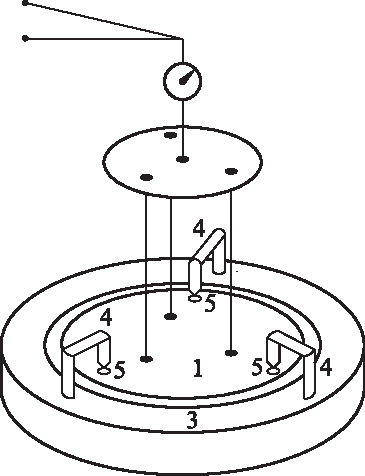
\includegraphics[width=0.38\textwidth]{1_2_2}
	\caption{Конструкция крепления подвижной пластины конденсатора}
	\labfigmark{voltmeter-capacitor}
\end{wrapfigure}

Измерения проводятся в условиях равновесия электрических и механических сил. Как следует из формулы (\r{2}),
электрические силы быстро возрастают с уменьшением зазора между пластинами. С другой стороны, механические силы,
обеспечивающие равновесие аналитических весов, возрастают при наклонах коромысла крайне медленно. В условиях нашего
опыта равновесие весов при равенстве электрических и механических сил оказывается поэтому неустойчивым.

При настройке прибора на левую чашку весов кладётся некоторый перегрузок. При этом положение весов фиксируется тремя
контактными винтами 4, расположенными в~вершинах равностороннего треугольника (\labfigref{voltmeter-experiment} и \r{2}). Винты упираются в
контактные площадки 5, установленные на верхней плоскости подвижной пластины. Напряжение на пластинах регулируется с
помощью реостата $R$ выпрямителя. Электрические силы, действующие на пластину 1, возрастают по мере увеличения
потенциала неподвижной пластины. В тот момент, когда эти силы сравниваются с~весом перегрузка, коромысло теряет
устойчивость и подвижная пластина <<прилипает>> к неподвижной. Этот момент фиксируется по движению стрелки весов.

\begin{lab:task}
	
	В работе предлагается исследовать связь между силой  притяжения пластин и разностью потенциалов между ними для
	определения электрической постоянной $\epsilon_0$ и коэффициента перевода единиц напряжения из системы СГС в систему СИ.
	
	\warning{Регулировка измерительного конденсатора требует определённых навыков и может производиться \important{только
	лаборантом или механиком}. Студент проверяет регулировку пластин визуально, не меняя их настройку самостоятельно.}
	
	\begin{enumerate}
		\item Перед началом работы рассчитайте по формуле (\r{2}) максимально допустимую нагрузку, исходя из предела измерений
		электростатического вольтметра. Расстояние между пластинами~$d$ и площадь пластин~$S$ указаны на установке.
		
		\item Соберите схему согласно Рис.~\ref{fig:voltmeter-experiment}.
		
		По уровню, расположенному на основании весов, проверьте, занимает ли платформа весов горизонтальное положение. При этом
		подвижная пластина измерительного конденсатора должна располагаться в~центре охранного кольца, не касаясь его. При
		обнаружении неисправностей обратитесь к лаборанту.
		
		Проверьте регулировку положения равновесия коромысла ненагруженных весов. Для этого следует отключить пластины
		конденсатора от выпрямителя и соединить их друг с другом (ключ К на Рис.~\ref{fig:voltmeter-experiment} переводится в нижнее положение). Осторожно,
		чтобы не сбить опорные призмы коромысла, освободите весы от арретира. В положении равновесия при закороченных пластинах
		упорные штифты должны быть близки к контактным пластинам и должны касаться их при незначительных ($\sim 10$~мг)
		перегрузках на левой чашке весов.
		
		При необходимости проведите регулировку положения коромысла весов. Для этого снова арретируйте весы и, перемещая
		тарировочные гайки, расположенные на концах коромысла, добейтесь того, чтобы стрелка весов оказалась на нулевом делении
		шкалы. Поворот гаек и изменение груза на чашке весов \important{всегда производятся при арретированных весах}, а проверка
		положения коромысла~--- когда весы сняты с арретира. Для изменения груза открываются боковые дверцы весов (фронтальная
		дверца открывается только на время ремонта).
		
		\item Исследуйте зависимость силы притяжения пластин от напряжения на конденсаторе. Для измерения напряжения применяется
		электростатический вольтметр (вольтметр, вмонтированный в выпрямитель, для измерений не используется).
		
		Переведите ключ К в положение измерения. Положите на левую чашку весов груз, равный примерно 0,1 от максимально
		допустимого. При этом подвижная пластина должна прижаться к упорным штифтам. Подберите напряжение, приводящее к потере
		устойчивости весов. Оно соответствует моменту начала движения стрелки весов.
		
		Рекомендуется уточнить это напряжение 2--3 раза, каждый раз всё медленнее поворачивая ручку реостата $R$. Перед каждым
		измерением напряжения следует закорачивать пластины конденсатора ключом К, чтобы снять с пластин остаточный заряд.
		
		Проведите такие измерения не менее чем в десяти точках, равномерно расположенных в рабочем диапазоне нагрузок.
		
		\item Сразу после измерений изобразите результаты на графике в координатах $F$, $U^2$. Если полученные точки в пределах
		ошибок опыта ложатся на прямую линию, эксперимент можно закончить. Если прямой линии не получилось, следует найти и
		устранить ошибку.
		
		\item По наклону прямой $F=f(U^2)$  рассчитайте значение электрической постоянной $\epsilon_0$.
		
		\item Используйте результаты измерений для определения коэффициента перевода единиц напряжения из системы СГС в систему СИ.
		Напряжение в единицах СГС может быть вычислено по формуле (\r{4}), а показания электростатического вольтметра позволяют
		определить это напряжение в вольтах. Изобразите полученные результаты на графике в координатах $U$~(в~СГС)$=f(U,~В)$ и по
		наклону прямой, проведённой через экспериментальные точки, определите коэффициент пересчёта напряжений.

	\end{enumerate}

\end{lab:task}

\begin{lab:questions}
	\item Оцените ошибку, возникающую вследствие того, что равновесие весов устанавливалось при наличии небольшого зазора между
	штифтами и контактными пластинами, а измерения производятся при отсутствии этого зазора.
	
	\item Покажите, что электростатический вольтметр пригоден для измерения как постоянного, так и переменного напряжения.
	
	\item Покажите, что измерения на переменном токе определяют именно эффективное значение его напряжения.
	
	\item Чем определяется интервал частот, в котором можно измерять переменные напряжения с помощью электростатического
	вольтметра?
\end{lab:questions}

\begin{lab:literature}
	\item {\em Сивухин Д.В.} Общий курс физики. Т.~III. Электричество --- М.: Наука, 1983, \S~125.
	
	\item {\em Калашников С.Г.} Электричество.~--- М.: Наука, 1977, \S\S~5, 6, 26.
	
	%\item {\em Кингсеп А.С., Локшин Г.Р., Ольхов О.А.} Основы физики. Т.~1. Ч.~III. Электричество и магнетизм.~--- М.:
	%Физматлит, 2001.
\end{lab:literature}



\lab{Измерение магнитного поля Земли}

\begin{lab:aim}
исследовать свойства постоянных неодимовых магнитов; 
измерить с помощью них горизонтальную и вертикальную составляющие индукции магнитного поля
Земли и магнитное наклонение.
\end{lab:aim}

\begin{lab:equipment}
неодимовые магниты; тонкая нить для изготовления 
крутильного маятника; медная проволока; электронные весы; секундомер; 
измеритель магнитной индукции; штангенциркуль; 
брусок, линейка и штатив из немагнитных материалов; 
набор гирь и разновесов.
\end{lab:equipment}


\labsection{Свойства точечного магнитного диполя}

Простейший магнитный диполь может быть образован витком с током или постоянным
магнитом. По определению, магнитный момент  $\vec{\mm}$
тонкого витка площадью $S$ с током $I$ равен (в системе СИ):
\begin{equation}\eqmark{p}
\vec{\mm}=I\vec S,
\end{equation}
где $\vec S = S\vec n$~--- вектор площади контура, образующий 
с направлением тока правовинтовую систему,  
$\vec n$~--- единичный вектор нормали к площадке
(это же направление $\vec{\mm}$ принимается за направление 
S\,$\to$\,N от южного S к северному N полюсу магнита). 
Если размеры контура с током
или магнитной стрелки малы по сравнению расстоянием до диполя, то
соответствующий магнитный диполь $\vec{\mm}$ называют 
\emph{элементарным} или \emph{точечным}. 

Магнитное поле точечного диполя определяется по формуле, 
аналогичной формуле для поля элементарного электрического диполя:
\begin{equation}\eqmark{Bp}
\vec B_{дип}= \frac{\mu_0}{4\pi}
\left(\frac{3(\vec{\mm}\cdot\vec r)\vec r}{r^5} - \frac{\vec{\mm}}{r^3}\right)
\end{equation}
(здесь $\mu_0/4\pi = 10^{-7}\;Н/А^2$).

Во внешнем магнитном поле с индукцией $\vec{B}$
на точечный магнитный диполь $\vec{\mm}$
действует механический момент сил:
\begin{equation}\eqmark{Mp}
\vec{\mathcal{M}}=\left[\vec{\mm}\times \vec B\right].
\end{equation}
При этом потенциальная энергия, которой обладает диполь с постоянным $\vec{\mm}$, 
равна 
\begin{equation}\eqmark{Wp}
W = -\left(\vec{\mm} \cdot \vec B\right).
\end{equation}
Когда диполь ориентирован вдоль внешнего поля ($\vec{\mm} \parallel \vec B$),
он находится состояния \emph{равновесия} ($\vec{\mathcal{M}} = 0$). При этом \emph{устойчивым}
будет только состояние, в котором диполь \emph{сонаправлен} с полем 
$\vec{\mm} \upuparrows \vec B$,
поскольку его потенциальная энергия достигает \emph{минимума} ($W_{\rm min} = - \mm B$).
При противоположной ориентации энергия будет иметь максимум 
($W_{\rm max}=\mm B$) и состояние равновесия будет неустойчивым.

\begin{lab:note}
        В системе СГС формулы \eqref{p}, \eqref{Bp} имеют соответственно вид
        \[
        \vec{\mm}=\frac{1}{c}I\vec S, \qquad 
        \vec B_{дип}= \frac{3(\vec{\mm}\cdot\vec r)\vec r}{r^5} - \frac{\vec{\mm}}{r^3}.
        \]
        Формулы \eqref{Mp} и \eqref{Wp} в СИ и СГС совпадают.
        
Последнее обстоятельство делает выражение \eqref{Wp} удобным для сопоставления единиц измерения 
магнитного момента $\mm$:
\begin{itemize}
\item СИ:  $\left[\mm\right]=\left[W\right]/[B]=\frac{Дж}{Тл}$;
\item СГС: $\left[\mm\right]=\left[W\right]/[B]=\frac{эрг}{Гс} = 
10^{-3}\frac{Дж}{Тл}$.
\end{itemize}
\end{lab:note}

В \emph{неоднородном} внешнем поле выражение для энергии постоянного диполя~\eqref{Wp} 
сохраняется. При этом кроме момента сил на диполь действует ещё и сила:
\begin{equation}\eqmark{Fp}
\vec F= -\nabla W = \left(\vec{\mm} \cdot \nabla\right)\vec B,
\end{equation}
где $\nabla=\left(\frac{{\partial}}{{\partial}x},
\,\frac{{\partial}}{{\partial}y},\,\frac{{\partial}}{{\partial}z}\right)$
--- векторный оператор <<набла>> (оператор Гамильтона). В частности, проекция
\eqref{Fp} на ось $x$ имеет вид
\[
F_x=\mm_{x} \frac{\partial B_{x}}{\partial x}+
\mm_{y} \frac{\partial B_{x}}{\partial y}+
\mm_{z} \frac{\partial B_{x}}{\partial z}.
\]

Таким образом, из \eqref{Mp}---\eqref{Fp} следует, что 
\emph{свободный} магнитный диполь в неоднородном магнитном поле
ориентируется вдоль силовых линий магнитного поля и втягивается в
область более сильного поля, поскольку это ведёт к уменьшению
энергии диполя.

Выражения~\eqref{Bp} и~\eqref{Fp} позволяют рассчитать силу взаимодействия
магнитов с моментами $\vec{\mm}_1$ и $\vec{\mm}_2$ в рамках модели точечных
диполей. В~частном случае, когда моменты двух небольших магнитов 
направлены вдоль соединяющей их прямой $\vec\mm_{1,2} \parallel \vec{r}$, 
где $\vec{r}$ --- радиус-вектор между ними, 
магниты  взаимодействуют с силой
\begin{equation} \eqmark{Fpp}
F_{12}=\mm_1\ppd{B_2}{r}=\mm_1\ppd{(2\mm_2/r^3)}{r}=-\frac{6\mm_1\mm_2}{r^4}
\quad (\text{ед. СГС}).
\end{equation}
(при использовании системы СИ \eqref{Fpp} нужно домножить на $\mu_0/4\pi$).
Здесь магниты притягиваются, если их магнитные моменты сонаправлены 
($\vec\mm_1 \upuparrows \vec\mm_2$) и отталкиваются, 
если направлены противоположно ($\vec\mm_1 \uparrow\downarrow \vec\mm_2$).

Если магнитные моменты направлены перпендикулярно соединяющей их прямой 
$\vec\mm_{1,2}\perp \vec{r}$, то нетрудно показать, что сила
их взаимодействия окажется в два раза меньшей и будет 
иметь противоположный знак: 
\[
F_{12}=\frac{3\mm_1\mm_2}{r^4} \qquad (\text{ед. СГС})
\]
(диполи притягиваются при  $\mm_1\uparrow \downarrow \mm_2$
 и отталкиваются при  $\mm_1\upuparrows \mm_2$).


\experiment

В работе используются неодимовые магниты
шарообразной формы.

\begin{lab:note}
<<Неодимовые>> магниты, состоящие из соединения
неодим-железо-бор (NdFeB), впервые были получены в 1983 году и 
на сегодняшний день являются самыми мощными постоянными магнитами.
С~их помощью которых можно поднимать грузы порядка тонны. 
Они нашли широкое применение в изготовлении 
жёстких дисков, DVD-приводов, звуковых динамиков, магнитных томографов и др.
\end{lab:note}

Для проведения эксперимента важно, что а) вещество, из которого изготовлены магниты, 
является \emph{магнитожёстким} материалом; б) шары намагничены однородно.

<<Магнитожёсткость>> материала (см. подробнее Раздел~IV) 
означает, что магнитные моменты шаров 
в процессе работы не изменяются под действием внешних магнитных полей, 
т.\,е. шар ведёт себя как постоянный (<<жёсткий>>) диполь. 
В том числе, магнитные моменты не изменяются при контакте магнитов друг
с другом.
%Поэтому, при расчетах можно считать, что шары взаимодействуют как
%жёсткие точечные магнитные диполи, расположенные в центрах шаров.

\etp{1.5}

Магнитное поле однородно намагниченного шара радиусом~$R$ может быть 
вычислено точно. На расстояниях $r{\geq}R$ от центра шара оно 
совпадает с полем \emph{точечного} магнитного диполя \eqref{Bp}, 
расположенного в центре, магнитный момент~$\vec\mm$ которого совпадает
с полным моментом шара. 
Внутри шара магнитное поле однородно: c помощью формулы 
\eqref{Bp} и условия непрерывности нормальной компоненты индукции
на поверхности шара нетрудно получить, что при $r < R$
\begin{equation}\eqmark{Bin}
\vec B_0 = \frac{\mu_0\vec \mm}{2\pi R^3}
\end{equation}
(в ед. СГС $\vec{B}_0 = 2 \vec \mm / R^3$).\pagebreak

В качестве ещё одной характеристики материала магнита используют остаточную
\term{намагниченность}~$\vec M$.
По определению, намагниченность равна \emph{объёмной плотности магнитного момента},
поэтому для однородно намагниченного шара
\begin{equation}
\vec\mm = \vec M V,
\end{equation}
где $V=\frac{4\pi}{3}R^3$ --- объём магнита. 
Величину $\vec B_r=\mu_0 \vec M$ называют \emph{остаточной индукцией} 
материала (в~ед.~СГС $\vec B_r = 4\pi \vec M$).

Из \eqref{Bp} нетрудно видеть, что индукция~$\vec B_p$ \emph{на полюсах} 
однородно намагниченного шара направлена по нормали к поверхности и
совпадает поэтому с индукцией внутри шара~$\vec B_p = \vec B_0$. 
Как следует из \eqref{Bin}, величина $B_p$ связана с остаточной 
индукцией $B_r$ соотношением
\begin{equation}\eqmark{BpBr}
B_p = B_0 = \frac{2}{3} B_r.
\end{equation}

\begin{lab:note}
Электрическим аналогом магнитного шара из магнитожёсткого материала является
диэлектрический шар, изготовленный из \textit{электрета}~--- материала с
<<замороженной>> поляризацией. По своей топологии внешнее поле шара из электрета
не отличается от поля постоянного шарообразного магнита. В электрическом поле 
он ведёт себя точно также, как магнитный шар в магнитном поле. 
Формулы, описывающие взаимодействие
постоянных шарообразных магнитов между собой и с магнитным полем, идентичны 
соотношениям для электрических диполей в электрическом поле.
\end{lab:note}

\labsection{Определение магнитного момента магнитных
шариков}

\labsubsection{Метод А}

\begin{wrapfigure}{o}{0.25\textwidth}
    \pic{\linewidth}{Chapter_1/1_3_1}
    \caption{Измерение магнитных моментов шариков}\figmark{1}
\end{wrapfigure}

Величину магнитного момента $\mm$ двух одинаковых шариков можно рассчитать, 
зная их массу $m$ и определив максимальное
расстояние  $r_{\mathrm{max}}$, на котором они ещё удерживают друг 
друга в поле тяжести (см. рис.~\figref{1}). 
При максимальном расстоянии сила тяжести шариков $mg$ равна силе их 
магнитного притяжения. Когда векторы двух магнитных моментов
ориентированы вертикально, из \eqref{Fpp} имеем:
\begin{equation}\eqmark{mmA}
\mm = \sqrt{\frac{mgr^4_{\rm max}}{6}}\qquad (\text{ед.~СГС}).
\end{equation}

По величине $\mm$ с помощью \eqref{Bp} 
можно рассчитать величину индукции~$\vec B$ вблизи любой точки на поверхности 
шара радиуса~$R$. Максимальная величина индукции наблюдаются на
полюсах (см.~\eqref{BpBr}).

\labsubsection{Метод Б}

\begin{wrapfigure}{i}{0.35\textwidth}
    \pic{\linewidth}{Chapter_1/1_3_2}
    \caption{Альтернативный метод измерения магнитных моментов шариков}\figmark{2}
\end{wrapfigure}
Величину магнитного момента шариков можно определить также 
по силе их сцепления. Она определяется как сила, необходимая для разрыва 
двух сцепившихся магнитных шариков. Сила сцепления максимальна, 
если шары  соединяются своими противоположными полюсами 
(магнитные моменты сонаправлены). 

Максимальную силу сцепления можно определить по весу магнитной цепочки, которую
способен удержать самый верхний магнитный шарик. Если цепь состоит из
одинаковых магнитных шариков (см. рис.~\figref{2}а), то при определённой 
длине она отрывается от верхнего шарика. При этом, учитывая, 
что сила притяжения убывает как  $F\propto 1/r^4$, где $r$~--- 
расстояния между центрами шаров, для рассчёта прочности цепочки 
достаточно учитывать силу взаимодействия верхнего шара с 3--4 ближайшими соседями. 

Сила сцепления \eqref{Fpp} двух одинаковых шаров радиусами~$R$ 
c магнитными моментами~$\mm$ равна 
\begin{equation}\eqmark{F0}
F_0=\frac{6\mm^2}{(2R)^4}=\frac{3\mm^2}{8R^4}\qquad (ед.~СГС).
\end{equation}
Тогда минимальный вес цепочки, 
при которой она оторвётся от верхнего шарика равен:
\begin{equation}\eqmark{FF}
F=F_0 \left(1 + \frac{1}{2^4} + \frac{1}{3^4}+ \frac{1}{4^4}+\ldots\right)\approx 1,08 F_0. 
\end{equation}
(мы ограничились четырьмя членами ряда; точность такого приближения предлагается
оценить самостоятельно). 
Отметим, что не обязательно составлять цепочку только из одинаковых шариков: на
расстояниях, превышающих 20--30 диаметров шариков, можно подцепить любой
груз, притягиваемый магнитом (см. рис.\figref{2}б),~--- 
на результат это не повлияет, в чём несложно убедиться экспериментально.

\labsection{Измерение горизонтальной составляющей индукции 
    магнитного поля Земли}

Магнитное поле Земли в настоящей работе измеряется 
по периоду крутильных колебаний <<магнитной стрелки>> вокруг вертикальной оси.

\begin{wrapfigure}[17]{o}{0.35\textwidth}
    \pic{\linewidth}{Chapter_1/1_3_3}
    \caption{Крутильный маятник во внешнем магнитном поле}\figmark{3}
\end{wrapfigure}
<<Магнитная стрелка>> образована сцепленными друг
с другом $n$ намагниченными шариками. С~помощью $\Lambda$-образного подвеса стрелка 
подвешена в горизонтальном положении (см. рис.~\figref{3}). 
Для крепления нити в работе используется штатив, изготовленный из немагнитного
материала. 

Магнитные моменты всех шариков направлены в одну сторону вдоль оси <<стрелки>>. Под действием
механического момента сил \eqref{Mp}, действующего на стрелку со стороны
поля Земли, стрелка стремится повернуться по горизонтальной составляющей 
магнитного поля Земли $\vec B_{\parallel}$ в направлении Юг---Север.


При отклонении стрелки на угол $\theta$ от равновесного положения 
в горизонтальной плоскости возникают крутильные колебания вокруг 
вертикальной оси, проходящей через середину стрелки. Если пренебречь 
упругостью нити, то уравнение крутильных колебаний такого маятника
определяется возвращающим моментом сил 
\[
\mathcal{M}=-\mm_n B_{\parallel}\sin \theta
\]
и моментом инерции $J_n$ <<стрелки>> относительно оси вращения. 
При малых амплитудах  $(\sin \theta \approx \theta)$ уравнение колебаний
стрелки имеет вид: 
\begin{equation*}
J_n \ddot{\theta} + \mm_n B_{\parallel} \theta = 0.
\end{equation*}
Отсюда находим период малых колебаний
\begin{equation}
T=2\pi \sqrt{\frac{J_n}{\mm_n B_{\parallel}}}.
\end{equation}

Здесь $\mm_n = n \mm$ --- полный магнитный момент магнитной <<стрелки>>, 
составленной из $n$ шариков.
Момент инерции $J_n$ стрелки из $n$ шариков с хорошей точностью равен 
моменту инерции тонкого однородного стержня массой $m_n = nm$
и длиной $\ell_n = n \cdot 2R$:
\begin{equation}\eqmark{Jn}
J_n \approx \frac{1}{12} m_n \ell_n^2 = \frac{1}{3}n^3 m R^2.
\end{equation}
%Даже для трёх шариков момент инерции, рассчитанный по приближённой формуле,
%отличается от точного результата (см. контрольный вопрос № 14) примерно на 2
%\%, а для  $n{\geq}5$~--- различие не превышает процента; если же учесть, что 
%$T\ \sqrt{I_n}$, то для всех  $n{\geq}3$\textit{ }погрешность наших расчетов
%для периода колебаний  $T$ не превысит процента, что освобождает нас от
%необходимости вводить поправочные коэффициенты.
Отсюда находим, что период колебаний маятника 
пропорционален числу шаров~$n$, составляющих <<стрелку>>:
\begin{equation}\eqmark{Tn}
T_n=2\pi \sqrt{\frac{mR^2}{3\mm B_{\parallel}}} \cdot n.
\end{equation}

При выводе \eqref{Tn} предполагалось, что магнитный момент~--- величина
\emph{аддитивная}: полный магнитный момент системы магнитов равен
векторной сумме магнитных моментов шариков.
Экспериментальное подтверждение этой зависимости $(T \propto n)$ будет являться
подтверждением справедливости предположений о магнитожёсткости материала
магнитов и, следовательно, аддитивности их магнитных моментов.

\labsection{Измерение вертикальной составляющей
индукции магнитного поля Земли. Магнитное наклонение.}

Для измерения вертикальной  $B_{\perp}$ составляющей вектора индукции поля Земли
используется та же установка, что и для измерения горизонтальной составляющей с
тем лишь отличием, что подвешенная магнитная <<стрелка>> 
закрепляется на нити в одной точке. 
В этом случае стрелка, составленная из чётного числа одинаковых шариков
и подвешенная за середину, расположится не горизонтально, 
а под некоторым углом к горизонту (см. рис.~\figref{4}а). 
Это связано с тем, что вектор~$\vec B$ индукции магнитного поля Земли 
не горизонтален, а образует с горизонтом некоторый угол~$\beta$, 
зависящий от географической широты  $\varphi$ места, где проводится опыт. 
Величина угла  $\beta $ называется \term{магнитным наклонением}.

\begin{figure}[h!]
    \centering
        \pic{8cm}{Chapter_1/1_3_4}
        \caption{Измерение вертикальной составляющей поля и магнитного наклонения}\figmark{4}
\end{figure}
      
Измерить магнитное наклонение непосредственно по положению подвешенной <<стрелки>>
затруднительно из-за механического момента нити в точке подвеса,
неизбежно возникающем при наклоне <<стрелки>>.
Избавиться от этого можно, если выровнять её горизонтально
с помощью небольшого дополнительного грузика (см. рис.~\figref{4}б).
В~этом случае момент силы тяжести
груза относительно точки подвеса будет равен моменту сил, действующих на
<<стрелку>> со стороны вертикальной составляющей магнитного поля Земли. 
Если масса уравновешивающего груза равна $m_{гр}$, плечо силы тяжести 
$r_{гр}$, а полный магнитный момент стрелки $\mm_n = n\mm$, то в равновесии: 
\begin{equation}\eqmark{mgr}
\mathcal{M}_n = m_{гр}gr_{гр}= n\mm B_{\perp}.
\end{equation}
Видно, что момент $\mathcal{M}_n$ силы тяжести уравновешивающего 
груза пропорционален числу $n$ шариков, образующих
магнитную <<стрелку>>: $\mathcal{M}\propto n$.

\begin{lab:warning}
    Магнитные предметы (ножницы, металлическая линейка, корпуса приборов,
    мобильные телефоны и др.), близко расположенные к экспериментальной установке, 
    могут существенно искажать результаты опыта по измерению индукции 
    магнитного поля Земли.
\end{lab:warning}


\begin{lab:task}

\taskpreamble{~}
\vspace*{-8ex} % workaround

\tasksection{I.~Определение магнитного момента, намагниченности и
остаточной магнитной индукции вещества магнитных шариков}

\item Измерьте диаметр шариков и взвесьте их на весах. Имейте ввиду, что весы могут давать
некорректные показания, если магниты класть непосредственно на платформу весов!

\item С помощью магнетометра измерьте индукцию поля $B_p$ на полюсах шарика. 
 
\item Проложите между двумя магнитными шариками брусок из немагнитного
материала. Подкладывая между бруском и верхним магнитиком листы бумаги 
(см. рис.~\figref{1}), определите, на каком максимальном 
расстоянии~$r_{\mathrm{max}}$ шарики удерживают друг друга в поле тяжести Земли. 

\item Рассчитайте величину магнитного момента магнитика $\mm$
(см. описание метода А). Оцените погрешность измерений.

\item Используя дополнительные шарики, составьте цепочку из 20--30 шариков и, 
с помощью неодимовых магнитов в форме параллелепипедов, подсоедините цепочку к
гире и разновесам, так, чтобы общая масса системы составила $\sim500$~г 
(рис.~\figref{2}б). 
Добавляя или удаляя шарики (шарики можно примагничивать непосредственно к
гире), подберите минимальный вес системы цепочки с гирей, 
при котором она отрывается от верхнего шарика. 

\item С помощью весов определите вес оторвавшейся цепочки с гирей.

\item Рассчитайте силу сцепления двух шаров 
и по ней определите магнитный момент шарика~$\mm$ (см. описание метода Б). 
Оцените погрешность результата.

\item Сравните значения магнитных моментов, полученные двумя методами. 
Какой метод даёт более точный результат?

\item Рассчитайте величину намагниченности материала шариков~$M$
и остаточную индукцию магнитного поля~$B_r$. 
Сравните значение~$B_r$ c табличными для соединения NdFeB.

\item Рассчитайте индукцию $B_p$ у полюсов шарика (см. \eqref{BpBr}). 
Сравните расчетное~$B_p$ значение с измеренным. 
При сильном расхождении результатов повторите измерения.

\tasksection{II.~Определение горизонтальной составляющей магнитного
поля Земли}

\item Соберите крутильный маятник (рис.~\figref{3}) из 12 магнитных шариков
и подвесьте его к немагнитному штативу.
Используя $\Lambda$-образный подвес, установите <<магнитную стрелку>>
 в горизонтальное положение (юстировка системы). 

\begin{figure}[h!]
   \centering
   \pic{1.9cm}{Chapter_1/1_3_5}
   \caption{Магнитная <<стрелка>>, свернутая в кольцо}\figmark{6}       
\end{figure}

\item Возбудите крутильные колебания маятника вокруг вертикальной оси 
и определите их период. Оцените влияние упругости (модуля кручения) нити 
на период колебаний, 
возбудив крутильные колебания <<стрелки>>, свёрнутой в кольцо 
(магнитный момент такого кольцеобразного маятника равен нулю) 
(см. рис.~\figref{6}). Убедитесь, что упругость нити при расчете 
периода колебаний можно не учитывать.

\item Исследуйте зависимость периода $T$ крутильных колебаний <<стрелки>> 
от количества магнитных шариков $n$, составляющих <<стрелку>>. Измерения
проведите для значений  $n=3,\,4,\,5,\,\dots,\,12$. Не забывайте для каждого
значения~$n$ юстировать систему, выставляя перед каждым измерением <<стрелку>>
горизонтально!

\item Постройте график экспериментальной зависимости $T(n)$.
Убедитесь в линейности этой зависимости. 
По значению углового коэффициента рассчитайте 
величину горизонтальной составляющей магнитного поля Земли (см. \eqref{Tn}).  
Оцените погрешность результата.

\tasksection{III. Определение вертикальной составляющей магнитного поля
Земли}

\item Изготовьте магнитную <<стрелку>> из $n=10$ шариков 
и подвесьте её за середину с помощью нити на штативе (см. рис.~\figref{4}а).
 
\item Определите механический момент сил, действующий со стороны магнитного поля
Земли на \emph{горизонтально} расположенную магнитную <<стрелку>>. 
Для этого, с помощью одного или нескольких кусочков проволоки, 
уравновесьте <<стрелку>> в горизонтальном положении
(см. рис.~\figref{4}б). 

\item С помощью весов определите массу уравновешивающего груза $m_{гр}$

\item Из условия равновесия рассчитайте механический момент сил~$\mathcal{M}$,
действующих на горизонтальную <<стрелку>> со стороны поля Земли. Измерения
момента сил проведите для чётных значений  $n= 4,\, 6,\, 8,\, 10,\, 12$.

\item  Постройте график экспериментальной зависимости
$\mathcal{M}(n)$. Убедитесь в линейности этой зависимости. 
Сделайте вывод о применимости приближения аддитивности
магнитных моментов для используемых в работе магнитов.
По значению углового коэффициента аппроксимирующей прямой 
рассчитайте величину вертикальной составляющей~$B_{\bot}$ магнитного
поля Земли. Оцените погрешность результата.

\item Используя результаты измерений  $B_{\perp}$ и  $B_{\parallel}$, 
определите магнитное наклонения~$\beta$ и полную величину индукции магнитного поля Земли на широте Долгопрудного. 

\item Сравните полученное значение наклонения $\beta$ с расчётным, 
в предположении, что магнитное поле Земли есть
поле однородно намагниченного вдоль оси вращения шара.
Оцените также полный магнитный момент~$\mm_{З}$ Земли.

\item Сравните полученные в работе результаты со справочными данными 
параметров магнитного поля Земли в Московском регионе.

\end{lab:task}

\begin{lab:questions}

\item Что такое магнитный момент? 
В~каких единицах он измеряется (в СИ и СГС)?

\item Какой ток $I$ должен циркулировать по плоскому витку радиусом, равным радиусу
используемых в работе магнитных неодимовых шариков, чтобы его магнитный момент
оказался равен магнитному моменту этих шариков? Расчёт проведите 
в системах СИ и СГС.

\item Какие силы действуют на точечный магнитный диполь 
в неоднородном внешнем магнитном поле?

\item По найденному в эксперименте значению магнитного момента неодимовых 
шариков, рассчитайте энергию и силу взаимодействия двух находящихся в контакте 
шариков, моменты которых ориентированных а)~вдоль, или б)~перпендикулярно соединяющих их прямой.

\item Как сила сцепления двух одинаковых неодимовых шарообразных магнитов 
зависит от их диаметров? Оцените силу сцепления двух 
неодимовых шаров диаметром $D=3$~см каждый. 

\item Покажите, что поле внутри однородно намагниченного шара 
радиуса  $R$ однородно и равно $\vec B_0=2\vec{\mm}/R^3$, 
где $\vec{\mm}$~--- полный магнитный момент шара. 

\item Найдите зависимость индукции магнитного поля  $B(\theta )$ 
от угла~$\theta $ вблизи поверхности однородно намагниченного шара 
(полярный угол $\theta $ отсчитывается от северного полюса шара).

%Найдите распределения токов намагничивания  $i(\theta )$ на поверхности
%однородно намагниченного шара ( $i$~--- линейная плотность поверхностных токов, 
%$\theta $~--- полярный угол). 

\item Приведите примеры материалов, используемых для изготовления 
постоянных магнитов. Каковы их характеристики? Используя табличные данные,
покажите, что намагниченность используемых в работе шариков можно 
считать практически постоянной.

\item Изменяется ли намагниченность постоянных магнитов с течением времени? 
Как размагнитить постоянный магнит? 
Как размагнитить намагниченный в поле магнита стальной инструмент 
(отвёртку,  пинцет)?

\item Получите точные значение момента инерции крутильного маятника  $J_n$
относительно оси вращения, составленного из  $n$ шариков и сравните
их с соответствующими значениями момента инерции, рассчитанными по приближённой
формуле для тонкого стержня \eqref{Jn}. При каком числе $n$
отличие будет составлять менее 1\%?

\item Для чего в конструкции крутильного маятника используется $\Lambda$-образный
подвес?

\item Получите формулу для периода крутильных колебаний горизонтальной магнитной
стрелки вблизи положения равновесия.

\item Поясните опыт, с помощью которого выясняется влияние упругости нити на
период крутильных колебаний.

\item Неодимовый шарообразный магнит диаметром $D=6$ см разрезали пополам. Какую
минимальную силу надо приложить, чтобы оторвать (без сдвига) одну половинку от
другой? 


\end{lab:questions}

\begin{lab:literature}
    \item \SivuhinIII~--- \S52, 57, 58, 74.
    \item \KingLokOlh~--- Ч.~II \S4.4, 5.3, 7.2.
    \item \Kirichenko~--- \S3.4, 4.2.
\end{lab:literature}




\cleardoublepage
\chapter{Электрические колебания}

\todo[inline,author=Tiffani]{Качество картинок в главе не очень.}

В этом разделе мы рассмотрим колебания токов (зарядов, напряжений) в
электрических цепях, включающих в себя резисторы, конденсаторы и катушки
индуктивности. Это --- свободные затухающие колебания в колебательном контуре, а
также вынужденные установившиеся колебания, возбуждаемые внешней ЭДС,
изменяющейся по синусоидальному закону. Изложение материала будет ориентировано
на его применение в лабораторном практикуме. Более детальное рассмотрение
электрических колебаний можно найти, например, в работах [1~--~5], ссылки на
которые даны в конце раздела.

Все колебания мы будем рассматривать при относительно низких частотах, когда
выполняется условие квазистационарности. Квазистационарность означает, что в
каждый момент времени значения тока~$I$ практически одинаковы во всех элементах
цепи, соединённых последовательно, то есть изменения токов во времени происходят
настолько медленно, что распространение электродинамических взаимодействий,
которое происходит со скоростью, близкой к скорости света в вакууме~$c$, можно
считать \important{мгновенным}. Условие квазистационарности выполнено, если
время~$\Delta t$ распространения электромагнитного возмущения на расстояние~$l$,
характеризующего геометрические размеры цепи, много меньше периода~$T$ колебаний
тока в контуре: $\Delta t=l/c\ll T$, или частота колебаний $\nu=1/T\ll1/\Delta
t$. Практически длина~$l$ совпадает с длиной провода, из которой изготовлена
обмотка катушки индуктивности. При $l=1$~м условие квазистационарности хорошо
выполняется при частотах $\nu\ll3\cdot10^8$~Гц.

Выполнение условия квазистационарности позволяет при расчёте цепей переменного
тока использовать закон Ома для замкнутой цепи и закон сохранения заряда так же,
как и при расчёте цепей постоянного тока. Следствием этих двух законов являются
два правила Кирхгофа. Первое правило: в каждой точке разветвления проводов
алгебраическая сумма токов равна нулю. Второе правило: для любого замкнутого
контура сумма падений напряжений на отдельных участках равна алгебраической
сумме ЭДС в этом контуре.

Ниже мы будем рассматривать, в основном, идеализированные цепи переменного тока,
в которых всё омическое сопротивление сосредоточено в резисторе,
некомпенсированные заряды расположены только на обкладках конденсатора, а всё
магнитное поле, связанное с током в цепи, локализовано в катушке индуктивности.
Более детальный учёт омических потерь в конденсаторах и катушках индуктивности
будет проведён в описаниях лабораторных работ, посвящённых изучению колебаний в
цепях переменного тока, где эти потери могут играть заметную роль.

Условие квазистационарности позволяет использовать связь между током~$I$ и
напряжением~$U$ на каждом из трёх элементов стандартной цепи:
для резистора с сопротивлением~$R$ напряжение
\begin{equation}
	\eqmark{2.1}
	U_R=IR;
\end{equation}
для конденсатора с ёмкостью~$C$ (когда ток~$I$ направлен к положительно
заряженной пластине):
\begin{equation}
	\eqmark{2.2}
	I=\dfrac{dq}{dt}=C\dfrac{dU_C}{dt};
\end{equation}
для катушки самоиндукции с индуктивностью~$L$:
\begin{equation}
	\eqmark{2.3}
	U_L=L\dfrac{dI}{dt}.
\end{equation}

В случае цепей постоянного тока правила Кирхгофа дают возможность получить
полную систему линейных алгебраических уравнений, из решения которой могут быть
найдены все неизвестные токи (заряды, напряжения). При расчёте цепи переменного
тока, используя эти правила для произвольного момента времени, мы получаем
систему линейных дифференциальных уравнений, которые позволяют найти временную
зависимость токов (зарядов, напряжений) в данной цепи. В частном случае, когда
речь идёт о вынужденных стационарных колебаниях, нет необходимости каждый раз
решать дифференциальные уравнения: для этих случаев используется стандартный
метод комплексных амплитуд или метод векторных диаграмм. Оба эти метода будут
рассмотрены ниже в пункте <<Вынужденные колебания>>.

\introsection{Свободные колебания}

Рассмотрим электрический контур, состоящий из последовательно соединённых
резистора~$R$, конденсатора~$C$ и катушки индуктивности~$L$
(рис.~\figref{fig1}).

\begin{figure}[h!]
	\centering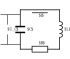
\includegraphics[width=0.3\linewidth]{Chapter_2/1}
	\caption{Колебательный контур.}
	\figmark{fig1}
\end{figure}
\todo[inline]{В старом тексте картинка такая же в лучшем качестве}


Сумма падений напряжения на элементах цепи в отсутствии внешней ЭДС равна нулю:
\begin{equation}
	\eqmark{2.4}
	RI+U_C+L\dfrac{dI}{dt}=0.
\end{equation}
Подставив в уравнение \eqref{2.4} выражения для~$I$ и $dI/dt$ из \eqref{2.2},
приходим к уравнению
\begin{equation}
	\eqmark{2.5}
	CL\dfrac{d^2U_C}{dt^2}+CR\dfrac{dU_C}{dt}+U_C=0.
\end{equation}
\todo[inline,author=Popov]{Промежуточные выкладки, на которые нет ссылки в тексте,
    должны идти без нумерации.}

Разделим это уравнение на~$CL$ и введём обозначения:
\begin{equation}\eqmark{2.6}
\gamma=\dfrac{R}{2L},~~~\omega_0^2=\dfrac{1}{LC},
\end{equation}
где $\gamma$~--- \important{коэффициент затухания},
$\omega_0$~--- \important{собственная круговая частота} колебательного контура.
Прилагательное  \important{<<круговая>>} в дальнейшем для сокращения записи
будем опускать. Введём также  \important{период собственных колебаний}~$T_0$:
\begin{equation}\eqmark{2.7}
T_0=\dfrac{2\pi}{\omega_0}=2\pi\sqrt{LC.}
\end{equation}
Уравнение для напряжения на конденсаторе~$U_C$ в колебательном контуре принимает
теперь вид:
\begin{equation}\eqmark{2.8}
\ddot{U}_C+2\gamma\dot{U}_C+\omega_0^2U_C=0,
\end{equation}
\todo[inline,author=Popov]{Выбор $U_C(t)$ в качестве основной величины
    сильно загромождает последующие выкладки. Почему бы не использовать
    заряд $q(t)$? Или обозначить просто $U(t)$?}
где точкой обозначено дифференцирование по времени. Легко показать, что так же
выглядят уравнения для других величин, характеризующих колебания в контуре.
Впрочем, решив уравнение \eqref{2.8}, можно получить выражение для тока~$I$ по
формуле \eqref{2.2}, заряда~$q$~--- по формуле~$q=CU_C$, а напряжений~$U_R$ и
$U_L$~--- по формулам \eqref{2.1} и \eqref{2.3}.

Отметим, что линейными дифференциальными уравнениями второго порядка вида
\eqref{2.8} описывается обширный класс колебательных систем как электрических,
так и механических. Механические колебания уже подробно изучались в рамках
семинарского и лабораторного практикумов, на что мы будем рассчитывать при
дальнейшем изложении, сокращая некоторые выкладки.

Для решения уравнения \eqref{2.8} введём новую переменную~$U(t)$, положив
\begin{equation}\eqmark{2.9}
U_C(t)=U(t)e^{-\gamma t}.
\end{equation}
\todo[inline,author=Popov]{Неудачное обозначение. Вместо $U(t)$ лучше $A(t)$ ---
    амплитуда колебаний.}
При этом из \eqref{2.8} получаем уравнение
\begin{equation}\eqmark{2.10}
\ddot{U}+\omega_1^2U=0,
\end{equation}
где
\begin{equation}\eqmark{2.11}
\omega_1^2=\omega_0^2-\gamma^2.
\end{equation}
В зависимости от соотношения между коэффициентом затухания~$\gamma$ и
собственной частотой~$\omega_0$ напряжение~$U_C$ по-разному меняется во времени.
Возможны три варианта, которые мы рассмотрим раздельно.

\introsubsection{Случай $0<\gamma<\omega_0$~--- затухающие колебания}
С учётом определений \eqref{2.6} условие реализации режима затухающих колебаний
в рассматриваемом $LCR$-контуре принимает вид:
\begin{equation}\eqmark{2.12}
0<R<2\sqrt{L/C}=2\rho=R_{\text{кр}},
\end{equation}
где введены ещё две характеристики колебательного контура:
\important{реактивное} или \important{волновое сопротивление} $\rho=\sqrt{L/C}$
и \important{критическое сопротивление} $R_{\text{кр}}$.
\todo[inline,author=Popov]{Колебательный контур --- квазистационарная система,
    в которой излучением и распространением волн пренебрегается.
    Термин ``волновое сопротивление'' для системы, в которой нет никаких волн~---
    не удачный. Кроме того, введение избыточной терминологии затрудняет восприятие текста.}
При выполнении условия
\eqref{2.12} из формулы \eqref{2.11} следует, что $\omega_1^2>0$ и, значит,
уравнение \eqref{2.10} описывает гармонические колебания величины $U(t)$ с
амплитудой~$U_0$, круговой частотой~$\omega_1$ и начальной фазой~$\varphi_0$:
\begin{equation}\eqmark{2.13}
U(t)=U_0\cos(\omega_1t+\varphi_0).
\end{equation}
Теперь с учётом формулы \eqref{2.9} для напряжения $U_C(t)$ на конденсаторе
можно записать решение исходного уравнения \eqref{2.8} в виде
\begin{equation}\eqmark{2.14}
U_C(t)=U_0e^{-\gamma t}\cos(\omega_1t+\varphi_0).
\end{equation}

В этом выражении, представляющем \important{затухающие колебания} напряжения на
конденсаторе $U_C(t)$, множитель $U_0e^{-\gamma t}$ перед периодической функцией
$\cos(\omega_1 t+\varphi_0)$ называется \important{амплитудой затухающих
колебаний}, а величина $\omega_1t+\varphi_0$~--- \important{фазой затухающих
колебаний}. Выражение \eqref{2.14} содержит две постоянные интегрирования
дифференциального уравнения \eqref{2.8}: \important{начальную амплитуду}~$U_0$ и
\important{начальную фазу}~$\varphi_0$, определяемые начальными условиями
задачи, то есть значениями амплитуды и фазы~$U_C(t)$ при~$t=0$. Величина
\begin{equation}\eqmark{2.15}
\omega_1=\sqrt{\omega_0^2-\gamma^2}
\end{equation}
в этом случае представляет \important{круговую частоту свободных}, или
\important{собственных, затухающих колебаний} (не путать с собственной частотой
$\omega_0$).

\todo[inline,author=Popov]{Выделить примеры отдельным стилем с мелким шрифтом.}
\begin{example}
В качестве примера рассмотрим случай, когда в начальный момент $(t=0)$ ток в
контуре $I(0)=0$, а напряжение на конденсаторе $U_C(0)=U_{C0}$, то есть
конденсатор имеет заряд $q(0)=q_0=CU_{C0}$. С~учётом \eqref{2.15} и \eqref{2.2}
это означает, что для уравнения \eqref{2.8} приняты начальные условия
\begin{equation}
	\eqmark{2.16}
		\begin{gathered}[c]
			U_C(0)=U_{C0}=U_0\cos\varphi_0, \\
			\dot{U}_C(0)=I(0)/C=-\gamma
U_0\cos\varphi_0-\omega_1U_0\sin\varphi_0=0.
		\end{gathered}
\end{equation}

Второе из условий \eqref{2.16} показывает, что $\tg\varphi_0=-\gamma/\omega_1$
и, следовательно,
\begin{equation}\eqmark{2.17}
\cos\varphi_0=\pm\omega_1/\omega_0, \qquad \sin\varphi_0=\mp\gamma/\omega_0.
\end{equation}
Выбор знака здесь не ограничивает общности решения. Выберем верхние знаки в
\eqref{2.17}. В этом случае при положительной постоянной интегрирования~$U_0$
после замыкания цепи, как станет видно из приведённых ниже формул, будет
происходить разрядка конденсатора. Начальные амплитуда~$U_0$ и фаза~$\varphi_0$
затухающих колебаний напряжения $U_C(t)$ на конденсаторе в представлении
\eqref{2.14} выражаются теперь через заданное начальное значение напряжения на
конденсаторе $U_{C0}$ и характеристики контура~$\gamma$ и~$\omega_1$:
\begin{equation}\eqmark{2.18}
U_C(t)=U_0e^{-\gamma t}\cos(\omega_1t+\varphi_0), \;
U_0=(\omega_0/\omega_1)U_{C0}, \; \varphi_0=-\arctg(\gamma/\omega_1).
\end{equation}
Для тока~$I(t)$ в контуре с учётом \eqref{2.2} получаем выражение в
представлении вида \eqref{2.14}:
\begin{equation}\eqmark{2.19}
I(t)=I_0e^{-\gamma t}\cos(\omega_1t+\pi/2), \qquad I_0=U_0/\rho,
\end{equation}
где~$I_0$ и~$\pi/2$~--- начальные значения амплитуды $I_0e^{-\gamma t}$ и фазы
затухающих колебаний тока соответственно.
\end{example}

\todo[inline,author=Popov]{Текст превращается в простыню. Нужна структура.}
\paragraph{Фазовые траектории.}
Заметим, что формулу \eqref{2.14} можно представить и в другом виде:
\begin{equation}\eqmark{2.20}
U_C(t)=e^{-\gamma t}(A\cos\omega_1 t+B\sin\omega_1 t),
\end{equation}
где две новые постоянные~$A$ и~$B$ связаны с постоянными~$U_0$ и~$\varphi_0$
соотношениями
\begin{equation}\eqmark{2.21}
A=U_0\cos\varphi_0, \qquad B=-U_0\sin\varphi_0.
\end{equation}
При этом окончательные формулы для напряжения~$U_C(t)$ и тока~$I(t)$, выраженные
через~$U_{C0}$ и характеристики контура, принимают вид:

\begin{equation}
	\eqmark{2.22}
		\begin{gathered}[c]
			U_C(t)=U_{C0}e^{-\gamma
t}[\cos\omega_1t+(\gamma/\omega_1)\sin\omega_1t], \\
			I(t)=C\dot{U}_C(t)
=-\left(U_{C0}/\rho\right)(\omega_0/\omega_1)e^{-\gamma t}\sin\omega_1t.
		\end{gathered}
\end{equation}
Из формул \eqref{2.22} следует параметрическое представление
\important{траектории системы на фазовой плоскости} переменных $U_C(t),
\dot{U}_C(t)=I(t)/C$. Задание этих двух величин полностью определяет состояние
системы в момент времени~$t$.

На рис.~\figref{fig2}a показаны \important{в безразмерных переменных}
зависимости \eqref{2.22} напряжения и тока в контуре от времени в режиме
свободных затухающих колебаний: сплошная линия $u(x)=U_C(x)/U_{C0}$, где
$x=(\omega_1/2\pi)t$, соответствует напряжению на конденсаторе $U_C(t)$, а
штриховая линия $j(x)=\rho I(x)/U_{C0}$~--- точку в контуре $I(t)$. На
рис.~\figref{fig2}б показана фазовая траектория этих колебаний на плоскости
переменных   $u(x),~j(x)$, представляющая собой скручивающуюся спираль.

\begin{figure}[h]
	\begin{minipage}[h]{0.5\linewidth}
		\center{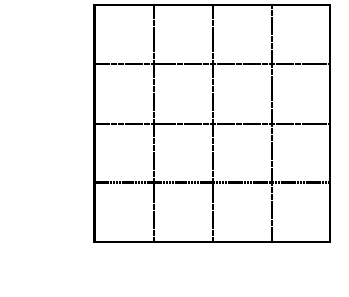
\includegraphics[width=1\linewidth]{Chapter_2/2} \\ а)}
	\end{minipage}
	\hfill
	\begin{minipage}[h]{0.5\linewidth}
		\center{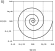
\includegraphics[width=0.9\linewidth]{Chapter_2/3} \\ б)}
	\end{minipage}
	\caption{(а,б). Затухающие колебания $(0<\gamma<\omega_0)$ при
$\gamma/\omega_0=0,1$.}
	\figmark{fig2}
\end{figure}

Из формул \eqref{2.14}, \eqref{2.19} и рис.~\figref{fig2} видно, что затухающие
при условии $0<\gamma<\omega_0$ колебания напряжения и тока не являются
периодическими функциями времени, однако эти величины дважды за время
\begin{equation}\eqmark{2.23}
T_1=\dfrac{2\pi}{\omega_1}=\dfrac{T_0}{\sqrt{1-\gamma^2/\omega_0^2}}
\end{equation}
проходят через нуль. А~так как согласно \eqref{2.2} нули функции $I(t)$ являются
нулями функции $dU_C/dt$, то величина~$T_1$ представляет также время между двумя
последовательными прохождениями напряжения $U_C(t)$ через максимум (минимум).
Очевидно, что экстремумы функции $I(t)$ чередуются с тем же периодом~$T_1$. Из
этих результатов возникает (с понятной долей условности) основание назвать
величину~$T_1$, определяемую формулами \eqref{2.23}, \important{периодом
затухающих колебаний}.

Взаимное расположение нулей и экстремумов $I(t)$ и~$U_C(t)$ легко понять из
энергетических соображений. Действительно, запасённая в контуре электромагнитная
энергия заключена в электрическом поле конденсатора и магнитном поле катушки
индуктивности, так что максимумы электрической энергии (экстремумы $U_C(t)$)
достигаются в нулях $I(t)$, а максимумы магнитной энергии (экстремумы $I(t)$)
достигаются в нулях $U_C(t)$.

Отметим, что все экстремумы не находятся на серединах временных интервалов между
соответствующими нулями, а сдвинуты влево на некоторую величину, возможность
определить которую предоставляется читателю.

Из формулы \eqref{2.23} следует, что $T_1>T_0$, то есть наличие потерь в
контуре, обусловленных сопротивлением~$R$ и представленных коэффициентом
$\gamma$, приводит к увеличению периода (уменьшению частоты) колебаний.

\todo[inline,author=Popov]{Текст превращается в простыню. Нужна структура.}
\paragraph{Характеристики затухающих колебаний.}
В~качестве характеристик процесса затухания колебаний помимо коэффициента
затухания~$\gamma$ используют \important{время затухания}
\begin{equation}\eqmark{2.24}
	\tau=1/\gamma=2L/R,
\end{equation}
то есть время, за которое амплитуда колебаний убывает в~$e$ раз, а также
\important{логарифмический декремент}
\begin{equation}\eqmark{2.25}
	\Theta=\ln\dfrac{U_{Ck}}{U_{C(k+1)}}=\ln e^{\gamma T_1}=\gamma T_1,
\end{equation}
\todo[inline,author=Popov]{Обозначение $U_{Ck}$ слишком громоздкое.
    Почему бы не использовать $A_k$?}
где $U_{Ck}$ и~$U_{C(k+1)}$~--- два последовательные максимальные отклонения
рассматриваемой величины (в данном примере - напряжения на конденсаторе) в одну
сторону от оси абсцисс. Из формул \eqref{2.24}, \eqref{2.25} следует связь между
логарифмическим декрементом~$\Theta$ и числом полных колебаний $N=\tau/T_1$ за
время затухания~$\tau$:
\begin{equation}\eqmark{2.26}
\Theta=1/N.
\end{equation}
Таким образом, логарифмический декремент затухания $\Theta$ равен обратному
числу~$N$ периодов~$T_1$, за которое амплитуда колебаний падает в~$e$ раз.

На практике для определения~$\Theta$ удобно использовать отношение максимальных
отклонений, разделённых целым числом~$n$ периодов~$T_1$ (см.
рис.~\figref{fig2}). В~этом случае формула для~$\Theta$ принимает вид:
\begin{equation}\eqmark{2.27}
\Theta=\dfrac{1}{n}\ln\dfrac{U_{Ck}}{U_{C(k+n)}}.
\end{equation}

Формулы \eqref{2.25}~--~\eqref{2.27} показывают, что максимумы (минимумы)
функции $U_C(t)$ образуют убывающую геометрическую прогрессию со знаменателем
\begin{equation}\eqmark{2.28}
U_{C(k+1)}/U_{Ck}=e^{-\Theta}.
\end{equation}
Такую же прогрессию образуют и экстремумы функции $I_C(t)$.

Логарифмический декремент определяет \important{шаг спирали затухающего
колебания} на фазовой плоскости. Действительно, из формулы \eqref{2.28} следует,
что
\begin{equation}\eqmark{2.29}
	U_{Ck}-U_{C(k+1)}=U_{Ck}\left(1-e^{-\Theta}\right).
\end{equation}
Рекомендуем читателю проверить, что кривые на рис.~\figref{fig2} соответствуют
$\gamma/\omega_0=0,1$.

С~логарифмическим декрементом связана ещё одна характеристика колебательного
контура~--- его \important{добротность}

\begin{equation}
	\eqmark{2.30}
		\begin{aligned}[c]
			Q&=\dfrac{\pi}{\Theta}=\dfrac{\pi}{\gamma T_1}=\pi
N=\frac{1}{2}\sqrt{\omega_0^2/\gamma^2-1} = \\
			&=\frac{1}{2}\sqrt{R_{\text{кр}}^2/R^2-1}=\sqrt{\rho^2/R^2-1/4}.
		\end{aligned}
\end{equation}

Как правило, о добротности говорят только тогда, когда добротность контура
достаточно велика, то есть $Q\gg1$. Такой добротностью обладают колебательные
контуры со \important{слабым} затуханием, представляющие большой практический
интерес. Для них вместо неравенств $0<\gamma<\omega_0$ и \eqref{2.12}
выполняются неравенства
\begin{equation}\eqmark{2.31}
0<\gamma\ll\omega_0,
\end{equation}
или, в терминах параметров контура,
\begin{equation}\eqmark{2.32}
0<R\ll2\sqrt{L/C}=2\rho=R_{\text{кр}}.
\end{equation}
Малость отношения $\gamma/\omega_0$ и связанных с ним характеристик контура:
\begin{equation}\eqmark{2.33}
\gamma/\omega_0=R/2\rho=R/R_{\text{кр}}\ll1,
\end{equation}
-- позволяет, пренебрегая вторыми и выше степенями в разложениях по этим малым
величинам, значительно упростить уже полученные формулы, например, \eqref{2.15},
\eqref{2.17}~--~\eqref{2.23}, \eqref{2.30}, и дальнейшие выкладки. Так, в этом
приближении можно заменить~$\omega_1$ и~$T_1$ соответственно на~$\omega_0$ и
$T_0$, связать добротность~$Q$ с другими характеристиками контура цепочкой
равенств
\begin{equation}\eqmark{2.34}
Q=\dfrac{\pi}{\gamma
T_0}=\dfrac{\omega_0}{2\gamma}=\dfrac{\tau\omega_0}{2}=\dfrac{\omega_0L}{R}
=\dfrac{1}{\omega_0CR}=\dfrac{1}{R}\sqrt{\dfrac{L}{C}}=\dfrac{\rho}{R},
\end{equation}
а напряжение на ёмкости и ток в контуре \eqref{2.22} представить в виде

\begin{equation}
	\eqmark{2.35}
		\begin{gathered}[c]
			U_C(t)=U_{C0}e^{-\gamma
                t}[\cos\omega_0t+\frac{\gamma}{\omega_0}\sin\omega_0t], \\
            I(t)=-\frac{U_{C0}}{\rho}e^{-\gamma t}\sin\omega_0 t.
		\end{gathered}
\end{equation}

\paragraph{Энергетический смысл добротности.}
В~энергетическом смысле добротность~$Q$ колебательной системы
(механической, электрической, оптической и т. д.) определяется как отношение
запасённой в ней энергии~$W_0$ к потере $\Delta W_1$ энергии за время $T/2\pi$, за
которое фаза колебания меняется на 1 радиан:
\begin{equation}\eqmark{2.36}
Q=\dfrac{W_0}{\Delta W_1}=2\pi\dfrac{W_0}{\Delta W_T},
\end{equation}
где  $\Delta W_T$~--- потеря энергии за период~$T$.
\todo[inline,author=Popov]{Не вполне ясно: мы доказываем энергетический смысл добротности
2.0.34 или определим новое понятие ``энергетической добротности''?}
При вычислении~$\Delta W_T$
воспользуемся формулами \eqref{2.22} для представленных на рис.~\figref{fig2}
затухающих колебаний в \emph{рассматриваемом} $LCR$-контуре. Тот факт, что
они получены для конкретных начальных условий ($U_C(0)=U_{C0}$, $I(0)=0$),
не скажется, естественно, на общности результата. Пусть в момент времени~$t_0$ ток
в контуре $I(t_0)=0$, а напряжение на конденсаторе экстремально: $U_C(t_0)=\pm
U_{C0}e^{-\gamma t_0}$. Тогда ток равен нулю и в момент $t_0+T_1$. В~эти моменты
времени в электрическом поле конденсатора сосредоточена вся энергия контура. При
этом потеря энергии
\begin{equation}
	\eqmark{2.37}
		\begin{gathered}[c]
			 \Delta W_T = W(t_0)-W(t_0+T_1)=(1-e^{-2\gamma T_1})W_0, \\
			 W_0 = e^{-2\gamma t_0}CU_{C0}^2/2.
		\end{gathered}
\end{equation}
\todo[inline,author=Popov]{Комбинация $CU_{C0}$ выглядит ужасно}

Формулы \eqref{2.37} справедливы и для моментов времени $t\ne t_0$, однако, как
уже говорилось выше при обсуждении нулей и экстремумов $I(t)$ и $U_C(t)$,
электромагнитная энергия в этом случае распределяется между конденсатором и
катушкой индуктивности, составляя в сумме величину $W(t)$.

В~случае \emph{слабого} затухания, когда выполняются неравенства
\eqref{2.31}, формулу \eqref{2.37} можно упростить. В~первом порядке по малому
параметру $\gamma/\omega_0 \Delta W_T\approx 4\pi(\gamma/\omega_0)W_0$, так что
\begin{equation*}
\Delta W_1=\frac{\Delta W_T}{2\pi}\approx \frac{2\gamma}{\omega_0}W_0.
\end{equation*}
Для <<энергетической>>
добротности \eqref{2.36} теперь приходим к формулам \eqref{2.34}, полученным в
случае \emph{слабого} затухания из введённого в общем случае
\emph{затухающих} колебаний выражения для добротности \eqref{2.30}.

\introsubsection{Случай $\gamma=\omega_0$~--- критический режим}
В этом варианте параметры контура связаны соотношениями
\begin{equation}\eqmark{2.38}
R=R_{\text{кр}}=2\sqrt{L/C}=2\rho,
\end{equation}
а уравнение \eqref{2.10} и его решение принимают вид: $\ddot{U}=0,
U(t)=A_1+A_2t$. Соответственно, напряжение на конденсаторе
\begin{equation}\eqmark{2.39}
U_C(t)=(A_1+A_2t)e^{-\gamma t},
\end{equation}
где постоянные интегрирования~$A_1$ и~$A_2$ определяются начальными условиями
задачи. Если, как и в \important{варианте 1}, приняты начальные условия:
$U_C(0)=U_{C0}$, $I(0)=0$,~--- то для напряжения на конденсаторе и тока в
контуре с учётом формул \eqref{2.9} и \eqref{2.2} получаем выражения:
\begin{equation}\eqmark{2.40}
U_C(t)=U_{C0}(1+\gamma t)e^{-\gamma t}, \qquad
I(t)=-\frac{U_{C0}}{\rho}\gamma t e^{-\gamma t}.
\end{equation}

Отметим, что на практике этот режим, требующий строгого выполнения условия
$\gamma=\omega_0$, не может быть точно реализован и имеет значение как
пограничный между режимом затухающих колебаний и рассматриваемого далее режимом
апериодического затухания.

\introsubsection{Случай $\gamma>\omega_0$~--- апериодический режим}
В~этом режиме $\omega_1^2=\omega_0^2-~\gamma^2<~0$, так что для
описания системы удобно перейти от тригонометрических функций к гиперболическим
функциям, введя вместо мнимой теперь величины~$\omega_1$ действительную величину
\begin{equation}\eqmark{2.41}
\alpha=\sqrt{\gamma^2-\omega_0^2}=\omega_0\sqrt{R^2/R_{\text{кр}}^2-1.}
\end{equation}
С~помощью подстановки нетрудно убедиться, что общее решение уравнения
\eqref{2.10} имеет при этом вид $U(t)=B_1e^{\alpha t}+B_2e^{-\alpha t}$, где
постоянные величины~$B_1$ и~$B_2$ определяются начальными условиями.
Соответственно, напряжение на конденсаторе
\begin{equation}\eqmark{2.42}
U_C(t)=e^{-\gamma t}(B_1e^{\alpha t}+B_2e^{-\alpha t}).
\end{equation}
При начальных условиях $U_C(0)=U_{C0}, I(0)=0$
\begin{equation}
	\eqmark{2.43}
		\begin{gathered}[c]
			U_C(t)=U_{C0}e^{-\gamma t}[\ch \alpha t+(\gamma/\alpha)\sh \alpha
t], \\
I(t)=-\frac{U_{C0}}{\rho}\frac{\omega_0}{\alpha}e^{-\gamma t}\sh \alpha t.
		\end{gathered}
\end{equation}

Как видно из \eqref{2.41}, апериодический режим реализуется, если параметры
контура удовлетворяют условию
\begin{equation}\eqmark{2.44}
R>R_{\text{кр}}=2\sqrt{L/C}=2\rho.
\end{equation}

Графики, соответствующие формулам \eqref{2.43}, а также фазовая траектория
системы в апериодическом режиме показаны в безразмерных переменных на
рис.~\figref{fig3} (a, б). На рис.~\figref{fig2}a сплошная линия
$u(x)=U_C(x)/U_{C0}$, где $x=\alpha t$, соответствует напряжению на конденсаторе
$U_C(t)$, а штриховая линия $j(x)=\rho I(x)/U_{C0}$~--- току в контуре $I(t)$.
На рис.~\figref{fig3}б показана фазовая траектория этих колебаний на плоскости
переменных $u(x),~j(x)$   при $\gamma/\omega_0=1,1~$, представляющая собой
короткий отрезок спирали.

\begin{figure}[h]
	\begin{minipage}[h]{0.49\linewidth}
		\centering{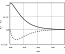
\includegraphics[width=1\linewidth]{Chapter_2/4} \\ а)}
		%\caption{а}
	\end{minipage}
	\hfill
	\begin{minipage}[h]{0.49\linewidth}
		\centering{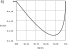
\includegraphics[width=0.9\linewidth]{Chapter_2/5} \\ б)}
		%\caption{б}
	\end{minipage}
	\caption{(а,б).Апериодический режим $(\gamma>\omega_0)$ при
$\gamma/\omega_0=1,1$.}
	\figmark{fig3}
\end{figure}

Как видно из рисунка, при выбранных начальных условиях в апериодическом режиме
на-пряжение на емкости убывает монотонно, а ток перед монотонным убыванием
совершает колебание, не меняя направления. Можно показать, что в этом режиме при
любых начальных условиях система стремится к равновесному состоянию
$U_C=0,~I=0$. При этом возможно не более одного прохождения через экстремальное
состояние, как на рис.~\figref{fig3}, и не более одного~--- через равновесное.

\introsection{Вынужденные колебания. Метод комплексных амплитуд. Векторные
диаграммы}

Рассмотрим процессы, протекающие в контуре, подключённом к источнику внешней
ЭДС, изменяющейся по гармоническому закону:
$\mathcal{E}=\mathcal{E}_0\cos(\omega t+\varphi_0)$. Соответствующая схема
представлена на рис.~\figref{fig4}.

\begin{figure}[h!]
	\centering
	\includegraphics[width=0.25\linewidth]{Chapter_2/6}
	\caption{Последовательный контур с внешней гармонической ЭДС}
	\figmark{fig4}
\end{figure}
\todo[inline,author=Popov]{Картинка совпадает с предыдущим изданием}

Потерями в конденсаторе и в катушке индуктивности в аналитических выкладках
будем пренебрегать, как и в п.1 при рассмотрении свободных колебаний. Потери в
катушке индуктивности учтём при рассмотрении векторных диаграмм.

Для напряжения на конденсаторе $U_C(t)$ вместо \eqref{2.8} получим теперь
уравнение
\begin{equation}\eqmark{2.45}
\ddot{U}_C+2\gamma \dot{U}_C+\omega_0^2U_C=\omega_0^2\mathcal{E}_0\cos(\omega t+
\varphi_0).
\end{equation}
Решение \important{линейного} дифференциального уравнения \eqref{2.45} с правой
частью состоит из общего решения однородного уравнения и какого-либо частного
решения данного уравнения с правой частью. Как показано в предыдущем разделе,
собственные свободные колебания контура (общее решение) при любых начальных
условиях экспоненциально затухают. Со временем их амплитуда становится
пренебрежимо малой, и в системе остаются только вынужденные колебания (частное
решение), обусловленные действием внешней ЭДС. Для нахождения этого частного
решения воспользуемся \important{методом комплексных амплитуд}. Данный метод
основан на следующем утверждении: \emph{пусть некоторая комплексная функция
является решением линейного дифференциального уравнения с вещественными
коэффициентами и комплексной правой частью; тогда вещественная часть этой
функции является решением того же уравнения, в правой части которого стоит
вещественная часть прежнего выражения, а мнимая часть~--- решением уравнения с
мнимой правой частью}.

Исходя из сказанного, перейдём к комплексному представлению колебаний и запишем
уравнение \eqref{2.45} в комплексной форме, отмечая комплексные величины
''стрелкой'':
\begin{equation*}
U_C=\Re \vec U_C, \quad \vec U_C=\Re \vec U_C+i\Im \vec U_C, \quad
\mathcal{E}=\Re \vec{\mathcal{E}}, \quad \vec{\mathcal{E}}=
\vec{\mathcal{E}}_0e^{i\omega t}=\mathcal{E}_0e^{i(\omega t+\varphi_0)},
\end{equation*}
\begin{equation}\eqmark{2.46}
\dfrac{d^2\vec U_C}{dt^2}+2\gamma\dfrac{d\vec U_C}{dt}+\omega_0^2\vec
U_C=\omega_0^2\mathcal{E}_0e^{i(\omega t+\varphi_0)}.
\end{equation}
Комплексная величина $\vec{\mathcal{E}}_0=\mathcal{E}_0e^{i\varphi_0}$, стоящая
перед $e^{i\omega t}$, называется \important{комплексной амплитудой} (в данном
случае это относится к внешней ЭДС). Решив уравнение \eqref{2.46}, мы получим
комплексное выражение для напряжения на конденсаторе. \important{Вещественная
часть} этого решения является, согласно приведённому выше утверждению, решением
исходного уравнения \eqref{2.45}.

Будем искать решение уравнения \eqref{2.46} в виде:
\begin{equation}\eqmark{2.47}
\vec U_C(t)=\vec U_{C0}e^{i\omega t},
\end{equation}
где $\vec U_{C0}$~--- комплексная амплитуда напряжения на конденсаторе, не
зависящая от времени. Подставляя \eqref{2.47} в \eqref{2.46} находим~$\vec
U_{C0}$, и далее, используя формулы \eqref{2.2}, \eqref{2.1},
\eqref{2.3},~--- комплексные амплитуды тока в контуре и напряжений на
сопротивлении и индуктивности:
\begin{subequations}
\renewcommand{\theequation}{\theparentequation \asbuk {equation}}
	\eqmark{2.48}
		\begin{equation}
			\eqmark{2.48a}
				\vec U_{C0}=(1/i\omega CZ)\mathcal{E}_0 e^{i\varphi_0}, \quad
Z=R+i(\omega L-1/\omega C)
		\end{equation}
		\begin{equation}
			\eqmark{2.48b}
			\begin{gathered}[c]
			\vec I_0=i\omega C\vec U_{C0}=(1/Z)\mathcal{E}_0 e^{i\varphi_0}, \\
			\vec U_{R0}=R\vec I_0=(R/Z)\mathcal{E}_0 e^{i\varphi_0}, \\
			\vec U_{L0}=i\omega L\vec I_0=(i\omega
L/Z)\mathcal{E}_0e^{i\varphi_0}
		\end{gathered}
		\end{equation}
\end{subequations}
\todo[inline,author=Popov]{Во всем разедел: сделать красивые формулы без лишних скобок.
    Сразу ввести обозначения так, чтобы громоздкие конструкции не возникали или
    хотя бы не повторялись.
Не выписывать лишний раз очевидные соотношения.}

Комплексная величина~$Z$ в формулах \eqref{2.48} называется
\important{комплексным сопротивлением}, или \important{импедансом},
последовательного контура и пишется обычно без ``стрелки''. Аналогичные
обозначения можно ввести и для отдельных элементов контура. Таким образом,
\begin{equation}
	\eqmark{2.49}
		\begin{gathered}[c]
			Z\equiv \Re  Z+i\Im Z=R+i(\omega L-1/\omega C), \\
			Z_R=R, \quad Z_L=i\omega L, \quad Z_C=-i/\omega C.
		\end{gathered}
\end{equation}
\todo[inline,author=Popov]{Здесь верхняя формула -- частный случай
    для последовательно соединённых RLC. Нижняя строка --- *общие*
    формулы для импедансов отдельных элементов каждого типа. Нужно разделить и подчеркнуть.}

В~этих обозначениях уравнения \eqref{2.48} принимают вид:
\begin{equation}
	\eqmark{2.50}
	\vec I_0=\vec{\mathcal{E}}_0/Z, \qquad \vec U_{R0}=Z_R\vec I_0, \qquad \vec
U_{C0}=Z_C\vec I_0, \qquad \vec U_{L0}=Z_L\vec I_0.
\end{equation}
Выражения \eqref{2.50} представляют обобщение закона Ома для переменных токов.
Роль сопротивлений в них играют импеданс контура~$Z$ в первом случае и импедансы
его отдельных элементов~--- в остальных случаях.

Важно отметить, что импеданс контура~$Z$ не зависит от начальных условий, не
содержит величин ни токов, ни напряжений, а определяется свойствами всех
элементов, соединённых в контур, и частотой синусоидальной ЭДС, к которой он
подключён. Таким образом, \important{импеданс~$Z$ является характеристикой
колебательного контура на заданной частоте}.

Выражение для~$Z$ содержит действительную часть $\Re Z=R$, называемую обычно
\important{активным сопротивлением} контура, и мнимую часть $\Im Z=\omega
L-1/\omega C$, носящую название \important{реактивного сопротивления}.
\emph{Правила сложения импедансов отдельных элементов схемы при
последовательном и параллельном включении~--- те же, что и для обыкновенных
сопротивлений}.

Импедансы реальных конденсаторов и катушек самоиндукции содержат кроме мнимой
части, также и действительную часть. Действительная часть импеданса определяется
необратимыми потерями энергии, которые могут быть связаны как с омическим
сопротивлением проводников, так и с другими причинами: с утечками и
диэлектрическими потерями в конденсаторах, с токами перемагничивания и токами
Фуко в магнитных сердечниках катушек самоиндукции. Потери в конденсаторах и в
катушках самоиндукции зависят как от частоты, так и от амплитуды проходящего
через них тока. Поэтому, приводя величины эквивалентного сопротивления потерь в
этих элементах, следует указывать частоту и амплитуду тока, при которых данные
величины были измерены.

Импедансы контура и его отдельных элементов~--- комплексные числа~--- могут быть
представлены в показательной форме. Для импеданса рассматриваемого
последовательного контура при этом находим:
\begin{subequations}
\renewcommand{\theequation}{\theparentequation \asbuk {equation}}
	\eqmark{2.51}
		\begin{equation}
			\eqmark{2.51a}
			Z=Z_0e^{i\psi_I}, \qquad Z_0=\sqrt{R^2+(\omega L-1/\omega
C)^2}=R/\cos\psi_I,
		\end{equation}
		\begin{equation}
			\eqmark{2.51b}
			\tg\psi_I=\Im Z/\Re Z=(\omega L-1/\omega C)/R, \quad
\psi_I=\arctg[(\omega L-1/\omega C)/R].
		\end{equation}
\end{subequations}
\todo[inline,author=Popov]{Обозначение $\psi_I$ ранее не определялось! Что это?}

Интересующие нас ток в контуре и напряжения на отдельных его элементах теперь
могут быть получены по формулам \eqref{2.48}~--- \eqref{2.50}. Например,
действительная часть тока в контуре
\begin{equation}
	\eqmark{2.52}
	I(t)=(\mathcal{E}_0/Z_0)\cos(\omega
t+\varphi_0-\psi_I)=(\mathcal{E}_0\cos\psi_I/R)\cos(\omega t+\varphi_0-\psi_I).
\end{equation}

Как видно из этой формулы, угол~$\psi_I$, определяемый отношением мнимой и
действительной частей импеданса, представляет собой сдвиг фаз между напряжением
на последовательном контуре и током в нём, причём \emph{положительные
значения угла~$\psi_I$ соответствуют отставанию фазы тока, а
отрицательные~--- опережению}. В~общем случае, когда к источнику последовательно
подключены резистор, конденсатор и катушка самоиндукции, сдвиг фазы тока
$\psi_I$ лежит в пределах $-\pi/2<\psi_I<\pi/2$. Из формулы \eqref{2.52} также
видно, что от угла~$\psi_I$ зависит амплитуда тока, а следовательно, и средняя
мощность активных потерь в контуре
\begin{equation}\eqmark{2.53}
	P=\langle I^2R\rangle_T=\mathcal{E}_0^2\cos^2\psi_I/2R,
\end{equation}
где угловые скобки с индексом <<$T$>> означают усреднение по периоду колебаний.
\todo[inline,author=Popov]{Все знают формулу с косинусом фи, а тут квадрат.
    Нужно как-то прокомментировать.

    Вообще стоит дать общий вывод связи мощности с комплексными амплитудами тока
    и напряжения. Эта формула важна и не очевидна. }

\todo[inline,author=Popov]{5 страниц текста без разбиения на структуру
    (позаголовки параграфов). Это не читаемо.}
\paragraph{Векторные диаграммы.}
Решения, полученные методом комплексных амплитуд, допускают простую
геометрическую интерпретацию. Комплексное число, например, напряжение
$\vec{\mathcal{E}}=\vec{\mathcal{E}}_0e^{i\omega t}=\mathcal{E}_0e^{i(\omega
t+\varphi_0)}$, представляется в комплексной плоскости вектором, длина которого
равна~$\mathcal{E}_0$~--- амплитуде напряжения $\mathcal{E}(t)$, а угол,
составляемый этим вектором с вещественной осью, равен $\omega
t+\varphi_0$~--- фазе напряжения $\mathcal{E}(t)$. Вектор $\vec{\mathcal{E}}$
вращается с угловой скоростью~$\omega$ против часовой стрелки. Удобно перейти к
системе координат, которая сама вращается с угловой скоростью~$\omega$. В~этой
системе вектор~$\vec{\mathcal{E}}$ будет представлен покоящимся вектором
$\vec{\mathcal{E}}_0=\mathcal{E}_0e^{i\varphi_0}$, а векторы~$\vec I_0$, $\vec U_{C0}$,
$\vec U_{R0}$ и~$\vec U_{L0}$ будут неподвижны, но окажутся сдвинутыми по углу
относительно вектора~$\vec{\mathcal{E}}_0$. Вектор~$\vec I_0$, как показано выше,
сдвинут от вектора~$\vec{\mathcal{E}}_0$ на угол~$\psi_I$, определяемый формулами
\eqref{2.51}.

Положения остальных векторов легко определить по формулам \eqref{2.48}. Так,
наличие множителя $i=exp(i\pi/2)$ в первом равенстве в \eqref{2.48b} означает,
что вектор~$\vec I_0$ опережает по углу на~$\pi/2$ вектор~$\vec U_{C0}$, то есть
ток опережает напряжение на конденсаторе по фазе на~$\pi/2$. Аналогично,
множитель $i=\exp(i\pi/2)$ в третьем равенстве в \eqref{2.48b} показывает, что
напряжение на индуктивности~$\vec U_{L0}$ опережает по фазе ток~$\vec I_0$ на
угол~$\pi/2$. Наконец, из второго равенства в \eqref{2.48b} видно, что вектор
$\vec U_{R0}$ совпадает по направлению с вектором~$\vec I_0$, и, значит,
напряжение на сопротивлении совпадает по фазе с током~$\vec I_0$. Построенные
таким образом диаграммы называются \important{векторными}.

В~качестве примера построим векторную диаграмму тока и напряжений для
последовательного контура. Рассмотрим схему, изображённую на рис.~\figref{fig5}.
К~источнику переменного напряжения $\mathcal{E}=\mathcal{E}_0\cos\omega t$
последовательно подключены резистор~$R$, катушка индуктивности~$L$,
действительная часть импеданса которой равна~$r_L$, и ёмкость~$C$. Активное
сопротивление~$r_L$ катушки индуктивности, которое с целью упрощения не
учитывалось выше при аналитическом решении задачи и будет учтено в описаниях
соответствующих лабораторных работ, легко может быть найдено в представленной на
рисунке <<схеме четырёх вольтметров>> с использованием векторной диаграммы.
Вольтметры измеряют напряжения на элементах цепи, амперметр измеряет ток.
Поскольку во всех элементах цепи ток~$I$ одинаков, удобно положить его фазу
равной нулю и отсчитывать от неё фазы напряжений на всех элементах цепи,
определив затем фазу   между напряжением на контуре и током.

\begin{figure}[h]
	\begin{minipage}[h]{0.37\linewidth}
		\centering{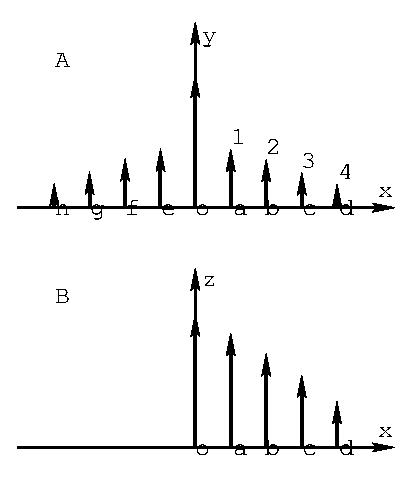
\includegraphics[width=1\linewidth]{Chapter_2/7} \\ а)}
		%\caption{а}
	\end{minipage}
	\hfill
	\begin{minipage}[h]{0.49\linewidth}
		\centering{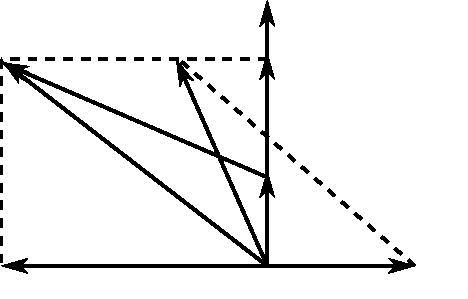
\includegraphics[width=1\linewidth]{Chapter_2/8} \\ б)}
		%\caption{б}
	\end{minipage}
	\caption{(а,б).Схема измерения (а) и векторная  диаграмма (б) для
последовательного контура}
	\figmark{fig5}
\end{figure}

Отложим вектор~$\vec I$ вдоль оси ординат (рис.~\figref{fig5}б). Напряжение на
резисторе совпадает по фазе с током, поэтому вектор~$\vec U_R$ также будет
направлен вдоль оси ординат. Напряжение на конденсаторе (без потерь) отстаёт по
фазе от тока на угол~$\pi/2$, поэтому вектор~$\vec U_C$ направлен
перпендикулярно вектору~$\vec I$ в сторону положительных значений абсцисс.
Векторное равенство напряжений $\vec U_{L+R}=\vec U_L+\vec U_R$ позволяет
построить треугольник по трём сторонам. Для этого сделаем две насечки:
первую~--- радиусом, равным модулю вектора $\vec U_{L+R}$, из начала этого
вектора (начала координат), вторую~--- радиусом, равным модулю вектора~$\vec
U_L$, из конца вектора~$\vec U_R$. Точка пересечения насечек определяет
положение векторов $\vec U_{L+R}$ и~$\vec U_L$ на диаграмме. Сложив векторы
$\vec{U}_{L+R}$ и~$\vec U_C$, получим вектор~$\vec{\mathcal{E}}$ входного
напряжения на контуре. Угол~$\psi_I$ показывает, каков сдвиг фаз между током и
напряжением в цепи. Разложим теперь вектор~$\vec U_L$ по осям координат.
Проекция~$\vec U_L$ на ось ординат позволяет определить $\vec
U_{L,\text{акт}}$~--- напряжение на активной части импеданса катушки, а проекция
на ось абсцисс даёт реактивную часть $\vec U_{L,\text{реакт}}$. Поделив эти
напряжения на ток~$I$, найдём действительную~$r_L$ и мнимую~$\omega L$ части
импеданса катушки.

\introsection{Вынужденные колебания. Резонанс}
\introsubsection{Резонанс напряжений в последовательном контуре}
В~предыдущем разделе были получены выражения \eqref{2.48}, описывающие в
комплексной форме вынужденные колебания в последовательном контуре под действием
внешней гармонической ЭДС. Там же указывалось, что эти колебания устанавливаются
в системе после затухания собственных свободных колебаний контура. Процесс
установления вынужденных колебаний будет рассмотрен отдельно в п.4 данного
раздела. Для исследования вынужденных колебаний и резонанса запишем
\important{вещественные части} решений \eqref{2.48}, использовав формулы
\eqref{2.7} и \eqref{2.12} для собственной частоты~$\omega_0$ и волнового
сопротивления~$\rho$, а также положив для сокращения записи раной нулю начальную
фазу:~$\varphi_0=0$. В~результате приходим к уравнениям:
\begin{subequations}
\renewcommand{\theequation}{\theparentequation \asbuk {equation}}
	\eqmark{2.54}
		\begin{equation}
			\eqmark{2.54a}
			I(t)=U_R(t)/R=I_{\omega}\cos(\omega t-\psi_I), \qquad
I_{\omega}=\mathcal{E}_0/Z_0,
		\end{equation}
		\begin{equation}
			\eqmark{2.54b}
			\begin{gathered}[c]
			Z_0=R\sqrt{1+(\rho/R)^2(\omega/\omega_0-\omega_0/\omega)^2},\\
			\psi_I=\arctg[(\rho/R)(\omega/\omega_0-\omega_0/\omega)],
			\end{gathered}
		\end{equation}
		\begin{equation}
			\eqmark{2.54c}
			U_C(t)=U_{C\omega}\cos(\omega t-\psi_C), \qquad
U_{C\omega}=\mathcal{E}_0\dfrac{\rho}{Z_0}\dfrac{\omega_0}{\omega}, \qquad
\psi_C=\psi_I+\pi/2,
		\end{equation}
		\begin{equation}
			\eqmark{2.54d}
			U_L(t)=U_{L\omega}\cos(\omega t-\psi_L), \qquad
U_{L\omega}=\mathcal{E}_0\dfrac{\rho}{Z_0}\dfrac{\omega}{\omega_0}, \qquad
\psi_L=\psi_I-\pi/2.
		\end{equation}
\end{subequations}
\todo[inline,author=Popov]{Нужно ли приводить ВСЁ это? Продраться через это невозможно.}

Отметим, что аналитическое выражение из \eqref{2.54b} для фазового сдвига
$\psi_I$ между внешней ЭДС и током в контуре легко упрощается в наиболее
интересной области, лежащей вблизи собственной частоты контура~$\omega_0$, а
фазовые сдвиги~$\psi_C$ и~$\psi_L$ связаны с~$\psi_I$ простыми соотношениями из
\eqref{2.54c} и \eqref{2.54d}. Напомним также, что согласно формуле \eqref{2.53}
от угла~$\psi_I$ зависит средняя мощность активных потерь в контуре.

Следует, однако, подчеркнуть, что в выражениях \eqref{2.54} не учтены
<<паразитные>> индуктивности и емкости реактивных элементов схемы, а также
возможные потери энергии в них. Необходимые уточнения будут сделаны в описаниях
соответствующих лабораторных работ.

Важно также отметить, что <<по умолчанию>> в нашем рассмотрении пренебрегалось
внутренним сопротивлением источника ЭДС, то есть считалось, что он является
\important{генератором напряжения}, который по определению обладает
\important{нулевым внутренним сопротивлением}. В~этом случае амплитуда
$\mathcal{E}_0$ не зависит от меняющегося с частотой сопротивления
нагрузки~--- последовательного колебательного контура.

Анализ формул \eqref{2.54} позволяет сделать следующие выводы.

1) При заданных параметрах~$\mathcal{E}_0$ и~$\omega$ внешнего источника
напряжения зависимости амплитуд и фаз тока и напряжений в системе от
частоты~--- \important{амплитудные} и \important{фазовые характеристики
системы}~--- определяются двумя безразмерными величинами: $\rho/R$ и
$\omega/\omega_0$. Как следует из формул \eqref{2.33}, \eqref{2.34}, для контура
со \important{слабым} затуханием, для которого добротность $Q\gg1$, отношение
$\rho/R=Q$, как уже отмечалось выше.

2) Поведение системы носит резонансный характер: при $\omega=\omega_0$, когда
мнимая часть импеданса контура $\Im Z=0$ и, соответственно,
%\setcounter{equation}{54}
\begin{equation}\eqmark{2.55}
	\omega_0L=1/\omega_0C=\rho,
\end{equation}
подкоренные выражения в формулах для амплитуд принимают минимальное значение,
равное единице, амплитуды тока и напряжения на сопротивлении достигают
максимальных значений
\begin{equation}\eqmark{2.56}
	I_{\omega_0}=\mathcal{E}_0/R, \qquad
U_{R\omega_0}=RI_{\omega_0}=\mathcal{E}_0
\end{equation}
и совпадают по фазе с ЭДС, поскольку~$\psi_0$. Таким образом, последовательный
контур на собственной частоте~$\omega_0$ представляет для внешней ЭДС чисто
активную нагрузку, на которой согласно \eqref{2.53} выделяется мощность
$P_{max}=\mathcal{E}_0^2/2R$.

3) Наиболее ярко резонансный характер вынужденных колебаний в
\important{последовательном} контуре проявляется в напряжениях на конденсаторе и
индуктивности, которые при $\omega=\omega_0$ в $\rho/R$ раз превышают напряжение
$\mathcal{E}_0$ по амплитуде и сдвинуты по фазе от него на $\mp\pi/2$
соответственно и, значит, находятся в противофазе друг с другом. Последние
утверждения, правда, относятся к идеальному случаю отсутствия потерь в этих
элементах. При добротности $Q=\rho/R\gg1$ амплитуды напряжений $U_C(t)$ и
$U_L(t)$ значительно превышают амплитуду~$\mathcal{E}_0$ напряжения на контуре.
По этой причине резонанс в последовательном контуре называется
\important{резонансом напряжений}.

4) Наличие множителей   в формулах \eqref{2.54c}, \eqref{2.54d} приводит к тому,
что \important{максимумы} напряжений на конденсаторе и индуктивности равны друг
другу, превышают $(\rho/R)\mathcal{E}_0$ и сдвинуты в разные стороны от
собственной частоты контура~$\omega_0$, на которой достигаются максимумы тока и
напряжения на сопротивлении~$R$:
\begin{equation}
	\eqmark{2.57}
	\begin{gathered}[c]
U_{C\omega_\text{m}}=U_{L\omega_\text{m}}=(\rho/R)\mathcal{E}_0[1-1/4(\rho/R)^2]
^{-1/2},\\
		\omega_{\text{m},C,L}=\omega_0[1-1/2(\rho/R)^2]^{\pm1/2}.
	\end{gathered}
\end{equation}
\todo[inline,author=Popov]{Может лучше так: $\mathcal{E}_0 \frac{Q}{\sqrt{1-Q^2/4}}$?
    И так везде.}
Рекомендуем читателям убедиться в этом самостоятельно.

Частоты, на которых достигаются \emph{максимальные} значения величин,
характеризующих вынужденные колебания в различных колебательных системах,
принято называть \important{резонансными}. Таким образом, в последовательном
колебательном контуре резонансной частотой для тока~$I$ и напряжения на
сопротивлении~$U_R$ является собственная частота контура~$\omega_0$, для
напряжения на конденсаторе~$U_C$~--- частота
$\omega_{\text{m}C}=\omega_0[1-1/2(\rho/R)^2]^{+1/2}$, для напряжения на
индуктивности~$U_L$~--- частота
$\omega_{\text{m}L}=\omega_0[1-1/2(\rho/R)^2]^{-1/2}$, причём
$\omega_{\text{m}C}\cdot\omega_{\text{m}L}=\omega_0^2$.

На рис.~\figref{fig6} приведены \important{в безразмерном виде} кривые
зависимостей от $x\equiv\omega/\omega_0$ амплитуды тока $j(x)\equiv
RI_\omega/\mathcal{E}_0$ (рис.~\figref{fig6} a) и амплитуды напряжения на
конденсаторе $u(x)\equiv U_{C\omega}/\mathcal{E}_0$  (рис.~\figref{fig6} б) при
трёх значениях отношения $\rho/R$, равных 2,~5 и 10.
\todo[author=Tiffani]{Нет подписи к рис. 2.6}
\begin{figure}[h]
	%\begin{center}
		\begin{minipage}[h]{0.45\linewidth}
			\centering{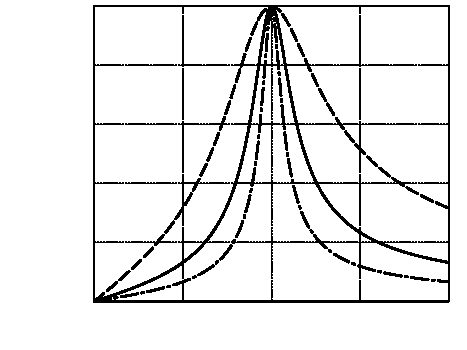
\includegraphics[width=1\linewidth]{Chapter_2/9} \\ а)}
			%\caption{а}
			%\figmark{fig6}
		\end{minipage}
		\hfill
		%\setcounter{figure}{5}
		\begin{minipage}[h]{0.45\linewidth}
			\centering{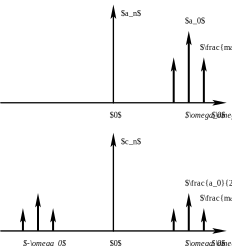
\includegraphics[width=1\linewidth]{Chapter_2/10} \\ б)}
			%\caption{б}
			%\figmark{fig9}
		\end{minipage}
	%\end{center}
		\caption{Нет подписи к рисунку}
		\figmark{fig6}
\end{figure}

Эти кривые называются \important{амплитудными резонансными кривыми}
колебательного контура. Важными характеристиками резонансных кривых являются
\important{максимальное значение амплитуды} соответствующей величины и
\important{ширина резонансной кривой}, при которой амплитуда этой величины
уменьшается в~$\sqrt{2}$ раз по сравнению со своим максимальным значением и в 2
раза уменьшается мощность сигнала. В~частности, по этим характеристикам можно
определить добротность колебательного контура. Например, эту величину можно
определить по отношению максимального значения напряжения на конденсаторе~$U_C$
к его статическому значению при~$\omega=0$, равному~$\mathcal{E}_0$, что следует
из формул \eqref{2.54} и видно из рис.~\figref{fig6}б.

Как уже отмечалось, о резонансе, как правило, говорят, если добротность~$Q$
колебательного контура достаточно велика и, следовательно, выполняются
соотношения \eqref{2.34}. Наибольший практический интерес представляет случай,
когда отклонение $\Delta\omega\equiv\omega-\omega_0$ частоты внешней ЭДС от
собственной частоты контура с добротностью $Q=\rho/R\gg1$ удовлетворяет сильному
неравенству
\begin{equation}\eqmark{2.58}
	|\Delta\omega|\ll\omega_0.
\end{equation}
При этом в первом порядке малости по \important{относительной расстройке
частоты} $\Delta\omega/\omega_0$
\begin{equation}\eqmark{2.59}
\dfrac{\omega}{\omega_0}-\dfrac{\omega_0}{\omega}=
\dfrac{2\Delta\omega}{\omega_0},
\end{equation}
что позволяет упростить выражения \eqref{2.54b} и представить их в виде:
\begin{subequations}
\renewcommand{\theequation}{\theparentequation \asbuk {equation}}
	\eqmark{2.60}
		\begin{equation}
			\eqmark{2.60a}
			Z_0=R\sqrt{1+(\tau\Delta\omega)^2}, \qquad
\psi_I=\arctg(\tau\Delta\omega),
		\end{equation}\\
		\text{где по определению \eqref{2.24} $\tau=1/\gamma$~--- время
затухания колебательного кон-}\\
		\text{тура.}\\
		\text{Соответственно упрощаются и выражения для амплитуд $I_{\omega}$,
$U_{C\omega}$ и $U_{L\omega}$ }\\
		\text{в остальных формулах \eqref{2.54}, в которые входит импеданс
контура $Z_0$:}
%костыль, но нормального работающего варианта со втавкой текста не придумала
		\begin{equation}
			\eqmark{2.60b}
			\begin{gathered}[c]
			I_{\omega}=\dfrac{\mathcal{E}_0}{R\sqrt{1+(\tau\Delta\omega)^2}},\\
U_{C\omega}=\dfrac{Q\mathcal{E}_0(\omega_0/\omega)}{\sqrt{1+(\tau\Delta\omega)^2
}},\\
U_{L\omega}=\dfrac{Q\mathcal{E}_0(\omega/\omega_0)}{\sqrt{1+(\tau\Delta\omega)^2
}}.
			\end{gathered}
		\end{equation}
\end{subequations}

На собственной частоте, когда $\omega=\omega_0,~\Delta\omega$, выражения для
амплитуд тока и напряжений на ёмкости и индуктивности, фазовых сдвигов и их
производных по частоте~$\omega$ принимают вид:
\begin{subequations}
\renewcommand{\theequation}{\theparentequation \asbuk {equation}}
	\eqmark{2.61}
		\begin{equation}
			\eqmark{2.54a}
			I_{\omega}(\omega_0)=U_{R\omega}(\omega_0)/R=\mathcal{E}_0/R, \qquad
\psi_I(\omega_0)=0,
		\end{equation}
		\begin{equation}
			\eqmark{2.54b}
			U_{C\omega}(\omega_0)=U_{L\omega}(\omega_0)=Q\mathcal{E}_0, \qquad
\psi_C(\omega_0)=-\psi_L(\omega_0)=-\pi/2,
		\end{equation}
		\begin{equation}
			\eqmark{2.54c}
			\psi'_I(\omega_0)=\psi'_L(\omega_0)=\psi'_C(\omega_0)=\tau.
		\end{equation}
\end{subequations}
Напомним, что максимальные (резонансные) значения напряжений на ёмкости и
индуктивности не строго равны~$Q\mathcal{E}_0$ и достигаются не строго на
частоте~$\omega_0$. Соответствующие относительные поправки, как это следует из
формул \eqref{2.57}, в рассматриваемом случае высокой добротности, когда
$Q\approx\rho/R\gg1$, составляют доли малой величины~$Q^{-2}$ и не учтены в
\eqref{2.61}.

\todo[inline,author=Popov]{Количество явно выписываемых формул нужно сократить. Очень трудно читать}

При отклонении $\Delta\omega=\omega-\omega_0=\Delta\omega{\gamma}$ таком, что
выполняется условие
%\setcounter{equation}{61}
\begin{equation}\eqmark{2.62}
\Delta\omega_{\gamma}=\pm\gamma, \quad \text{или} \quad
\tau\Delta\omega{\gamma}=\pm1,
\end{equation}
амплитуда тока~$I_{\omega}$, как видно из формул \eqref{2.60}, уменьшается в
$\sqrt{2}$ раз относительно своей максимальной (резонансной) величины, а фаза
$\psi_I$ изменяется на угол $\pm\pi/4$. Аналогичные изменения происходят с
амплитудами $U_{C\omega},~U_{L\omega}$ и фазами~$\psi_C$, $\psi_L$   напряжений на
ёмкости и индуктивности: амплитуды уменьшаются в~$\sqrt{2}$ раз, а фазы меняются
на угол~$\pm\pi/4$ по отношению к своим резонансным значениям.

Величина $\delta\omega\equiv2|\Delta\omega_{\gamma}|=2\gamma=2/\tau$
представляет собой важную характеристику колебательного
контура~--- \important{ширину резонансной кривой} $U_C(\omega)$, по которой с
учётом соотношений $Q=\omega_0/2\gamma=\tau\omega_0/2$ из \eqref{2.34}, зная
резонансную частоту~$\omega_0$, можно найти добротность контура
\begin{equation}\eqmark{2.63}
Q=\dfrac{\omega_0}{\delta\omega}.
\end{equation}

Ширину резонансной кривой и добротность можно определить и по
фазово-частотным характеристикам контура. Например, тангенс угла наклона
кривой $\psi_C(\omega)$ в точке резонанса согласно \eqref{2.54c} равен времени
затухания $\tau=2/\delta\omega$, а расстояние по оси~$\omega$ между точками, в
которых фаза~$\psi_C$ меняется от~$\pi/4$ до~$3\pi/4$, равно
$2/\tau=\delta\omega$.

Следует отметить, что в соотношении $\tau\cdot\delta\omega\sim1$, которому
подчиняется произведение времени затухания и ширины резонансной кривой
колебательного контура, проявляется фундаментальное \important{соотношение
неопределённости}, связывающее, в частности, <<время жизни>>~$\tau$ квантового
осциллятора с шириной спектральной линии~$\delta\omega$ его излучения (см.,
например, [1], с.~390).
\todo[inline,author=Popov]{Зачем квантового? В данном контексте это классическое
    соотношение для связи ширины спектра и длительности импульса. Дать ссылку на раздел 6}

\introsubsection{Резонанс токов в параллельном контуре}

Рассмотрим теперь вынужденные колебания в параллельном контуре, одна из ветвей
которого содержит индуктивность~$L$ и сопротивление~$R$, а другая~--- ёмкость
$C$ (рис.~\figref{fig7}).
\begin{center}
	\begin{figure}[h!]
		\centering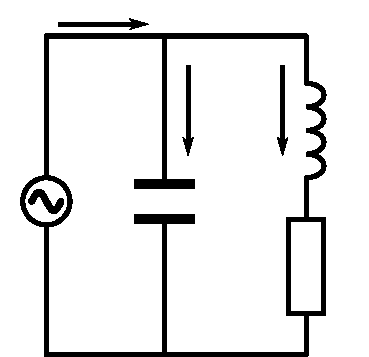
\includegraphics[width=0.25\linewidth]{Chapter_2/11}
		\caption{Параллельный контур с внешней гармонической ЭДС}
		\figmark{fig7}
	\end{figure}
\end{center}

Контур подключён к источнику ЭДС, задающему во внешней цепи ток, изменяющийся по
гармоническому закону: $I=I_0\cos(\omega t+\varphi_0)$. Таким образом, мы
предполагаем, что внутреннее сопротивлением источника столь велико, что он
является \important{генератором тока}, который по определению обладает
\important{бесконечно большим внутренним сопротивлением}. Потерями в катушке
индуктивности и конденсаторе будем пренебрегать, как это делалось и при
рассмотрении резонанса напряжений в последовательном контуре. Необходимые
уточнения будут сделаны в описаниях соответствующих лабораторных работ.

Воспользовавшись формулами \eqref{2.49}, правилами сложения сопротивлений и
правилами Кирхгофа, для комплексных амплитуд токов в ёмкостной~$\vec I_C$ и
индуктивной~$\vec I_L$ ветвях контура, а также для напряжения~$\vec U$ на
контуре, совпадающем в нашем приближении с напряжением на конденсаторе, при
начальной фазе $\varphi_0=0$ тока $\vec I=I_0e^{i\varphi_0}$ во внешней цепи
получаем выражения:
\begin{subequations}
\renewcommand{\theequation}{\theparentequation \asbuk {equation}}
	\eqmark{2.64}
		\begin{equation}
			\eqmark{2.64a}
			\vec I_C=\vec
I\dfrac{Z_{LR}}{Z_C+Z_{LR}}=i\dfrac{\rho\omega}{R\omega_0}I_0\dfrac{
1-iR\omega_0/\rho\omega}{1+i(\rho/R)(\omega/\omega_0-\omega_0/\omega)},
		\end{equation}
		\begin{equation}
			\eqmark{2.64b}
			\vec I_L=\vec
I\dfrac{Z_C}{Z_C+Z_{LR}}=-i\dfrac{\rho\omega_0}{R\omega}I_0\dfrac{1}{
1+i(\rho/R)(\omega/\omega_0-\omega_0/\omega)},
		\end{equation}
		\begin{equation}
			\eqmark{2.64c}
			\vec U=\vec IZ=\vec
I\dfrac{Z_CZ_{LR}}{Z_C+Z_{LR}}=\dfrac{\rho^2}{R}I_0\dfrac{
1-iR\omega_0/\rho\omega}{1+i(\rho/R)(\omega/\omega_0-\omega_0/\omega)},
		\end{equation}
\end{subequations}
где~$Z_C$ и~$Z_{LR}$~--- импедансы емкостной и индуктивной ветвей параллельного
контура соответственно.
\todo[inline,author=Popov]{Необходимо переобозначить и упростить. Либо не выписывать всё.}

Ограничимся рассмотрением наиболее интересного случая контура с высокой
добротностью вблизи резонансной частоты, когда $Q=\rho/R\gg1$, выполняется
условие \eqref{2.58} и применимо разложение \eqref{2.59}. При этом
\important{вещественные части комплексных амплитуд} \eqref{2.64} можно
представить в виде
\begin{subequations}
\renewcommand{\theequation}{\theparentequation \asbuk {equation}}
	\eqmark{2.65}
		\begin{equation}
			\eqmark{2.65a}
			I_C(t)=QI_0\dfrac{\omega}{\omega_0}\dfrac{\cos(\omega
t-\psi_C)}{R\sqrt{1+(\tau\Delta\omega)^2}}, \qquad
\psi_C=\arctg(\tau\Delta\omega)-\dfrac{\pi}{2}+Q^{-1},
		\end{equation}
		\begin{equation}
			\eqmark{2.65b}
			I_L(t)=QI_0\dfrac{\omega_0}{\omega}\dfrac{\cos(\omega
t-\psi_L)}{\sqrt{1+(\tau\Delta\omega)^2}}, \qquad
\psi_L=\arctg(\tau\Delta\omega)+\dfrac{\pi}{2},
		\end{equation}
		\begin{equation}
			\eqmark{2.65c}
			U(t)=Q\rho I_0\dfrac{\cos(\omega
t-\psi_U)}{\sqrt{1+(\tau\Delta\omega)^2}}, \qquad
\psi_U=\arctg(\tau\Delta\omega)+\dfrac{\omega_0}{\omega}Q^{-1}.
		\end{equation}
\end{subequations}

При резонансе, когда в принятом выше приближении
$\omega=\omega_0,~\Delta\omega=0$, амплитуды токов в ветвях контура, напряжения
на нём, фазовые сдвиги и их производные по циклической частоте~$\omega$
принимают вид:
\begin{subequations}
\renewcommand{\theequation}{\theparentequation \asbuk {equation}}
	\eqmark{2.66}
		\begin{equation}
			\eqmark{2.66a}
			I_{C\omega}=QI_0, \quad \psi_C(\omega_0)=-\dfrac{\pi}{2}+Q^{-1},
\quad I_{L\omega}(\omega_0)=QI_0, \quad \psi_L(\omega_0)=\dfrac{\pi}{2},
		\end{equation}
		\begin{equation}
			\eqmark{2.66b}
			U_{\omega}(\omega_0)=Q\rho I_0=Q^2RI_0, \qquad
\psi_U(\omega_0)=Q^{-1},
		\end{equation}
		\begin{equation}
			\eqmark{2.66c}
			\psi'_C(\omega_0)=\psi'_L(\omega_0)=\psi'_U(\omega_0)=\tau.
		\end{equation}
\end{subequations}
Из формул \eqref{2.63} следует, что на частоте~$\omega_0$ токи~$I_C$ и~$I_L$ в
ёмкостной и индуктивной ветвях контура в~$Q$ раз превышают ток~$I$ во внешней
цепи. При этом ток~$I_C$ опережает внешний ток~$I$ по фазе почти на~$\pi/2$, а
ток~$I_L$~--- отстаёт на~$\pi/2$. Между собой токи~$I_C$ и~$I_L$ сдвинуты по
фазе на угол, близкий к~$\pi$. Можно сказать, что токи~$I_C$ и~$I_L$ образуют
контурный ток, последовательно обтекающий элементы контура и в~$Q$ раз
превышающий по амплитуде внешний ток~$I$. Последнее обстоятельство послужило
поводом назвать резонанс в параллельном контуре \important{резонансом токов}.

Отметим, однако, что максимальные значения токов в контуре не строго равны
$QI_0$ и достигаются не строго на частоте~$\omega_0$. Соответствующие
относительные поправки, как и в случае резонанса напряжения, обусловлены
входящими в выражения \eqref{2.65}, \eqref{2.65b} для токов~$I_C$, $I_L$
множителями $(\omega_0/\omega)^{\pm1}$ и составляют доли малой величины
$Q^{-2}$.

Из формул \eqref{2.64b} вытекает, что на частоте~$\omega_0$ импеданс контура
$Z(\omega_0)=\vec U(\omega_0)/I_0$ является почти чисто активным. В
пренебрежении относительными поправками порядка~$Q^{-2}$ его модуль и фаза
относительно внешнего тока соответственно равны:
\setcounter{equation}{66}
\begin{equation}\eqmark{2.67}
|Z(\omega_0)|=Q\rho=Q^2R=\rho^2/R, \qquad \psi_Z(\omega_0)=Q^{-1}.
\end{equation}
Как видим, сопротивление контура в резонансе в~$Q^2$ раз превышает его активное
сопротивление~$R$. Это свойство параллельного контура широко используется в
радиотехнике.

По формулам \eqref{2.66a}, \eqref{2.66b} легко построить векторную диаграмму для
резонанса токов в рассмотренном выше параллельном контуре, в котором не
учитывались потери в конденсаторе и катушке индуктивности. Такая диаграмма
представлен на рис.~\figref{fig8}.

\begin{figure}[h!]
	\centering\includegraphics[width=0.5\linewidth]{Chapter_2/12}
	\caption{Векторная диаграмма при резонансе токов}
	\figmark{fig8}
\end{figure}

По оси ординат отложен внешний ток~$\vec I$. Напряжение на конденсаторе, равное
напряжению на контуре~$\vec U$, с учётом принятого правила знаков отстаёт по
фазе от тока~$\vec I$ на угол~$Q^{-1}$. Ток~$\vec I_C$ через конденсатор (без
потерь) опережает по фазе напряжение~$\vec U$ на~$\pi/2$. Ток через
индуктивность~$\vec I_L$ отстаёт от внешнего тока~$\vec I$ по фазе на~$\pi/2$.
Напряжение~$\vec U_R$ на сопротивлении совпадает по фазе с током~$\vec I_L$,
напряжение~$\vec U_L$ на индуктивности (без потерь) опережает ток~$\vec I_L$ на
$\pi/2$. Как видим, контур с активными потерями только в индуктивной ветви
проявляет ёмкостную реакцию: напряжение на контуре отстаёт по фазе от тока. Учёт
потерь в катушке индуктивности и конденсаторе несколько изменит векторную
диаграмму на рис.~\figref{fig8}, что будет рассмотрено в соответствующих
лабораторных работах.

Таким образом, условия резонанса токов в параллельном контуре и резонанса
напряжений в последовательном высокодобротном контуре совпадают:
$\omega=\omega_0$. Но, если в последовательном контуре резонансное сопротивление
контура равно чисто активному сопротивлению цепи~$R$ и минимально, обеспечивая
максимум тока при заданном внешнем напряжении, то в параллельном контуре
резонансное сопротивление контура почти чисто активное, обратно
пропорционально~$R$ и в~$Q^2$ раз его превышает, обеспечивая максимум напряжения
на контуре при заданном внешнем токе. Сдвиг фаз между напряжением и током при
резонансе напряжений всегда отсутствует, а при резонансе токов он близок к нулю
только, если $Q\gg1$. Впрочем, как правило, о резонансе и добротности говорят
только тогда, когда добротность контура достаточно велика.

\introsection{Установление вынужденных колебаний}

Рассмотрим процесс установления вынужденных колебаний в
\important{выскодобротном последовательном контуре}. Общее решение уравнения
\eqref{2.46} представляет собой сумму решения \eqref{2.14}, содержащего две
постоянные, зависящие от начальных условий задачи, и частного решения
\eqref{2.54c}. При наличии внешнего источника в качестве начальных естественно
выбрать <<нулевые>> условия: $U_C(0)=0,~\dot U_C(0)=0$, а решение искать в виде
\begin{equation}
	\eqmark{2.68}
	U_C(t)=U_{C\omega}\sin(\omega t-\psi_I)-U_0e^{-\gamma
t}\sin(\omega_1t-\varphi_0),
\end{equation}
где $U_{C\omega}$ и~$\psi_I$~--- зависящие от частоты~$\omega$ амплитуда и фаза
вынужденных колебаний, определяемые формулами \eqref{2.54}. Из начальных условий
при этом получаем систему уравнений, которая позволяет найти постоянные величины
$U_0$ и~$\varphi_0$:
\begin{equation}
	\eqmark{2.69}
	U_{C\omega}\sin\psi_I=U_0\sin\varphi_0, \qquad
U_{C\omega}\omega\cos\psi_I=U_0(\gamma\sin\varphi_0+\omega_1\cos\varphi_0).
\end{equation}
Для резонансного случая $\omega=\omega_0$, когда согласно \eqref{2.54}
$\psi_I=0$, а $U_{C\omega}=Q\mathcal{E}_0$, из уравнений \eqref{2.69} получаем
искомые константы $\varphi_0=0$ и $U_0=Q\mathcal{E}_0\omega_0/\omega_1$, а далее
из уравнения eqref{2.68}~--- \important{точное решение} задачи об установлении
вынужденных колебаний на резонансной частоте в последовательном контуре с
высокой добротностью при <<нулевых>> начальных условиях:
\begin{equation}
	\eqmark{2.70}
	U_{C}(t)=Q\mathcal{E}_0[\sin\omega_0t-(\omega_0/\omega_1)e^{-\gamma
t}\sin\omega_1 t].
\end{equation}
В общем случае при $\omega_1\approx\omega_0$ уравнение такого вида описывает
\important{биения} двух гармонических сигналов \important{близких} частот с
экспоненциально убывающей амплитудой одного из них. Появление биений связано с
тем, что разность фаз этих сигналов медленно меняется со временем:
$\Delta\varphi=(\omega_0-\omega_1)t$,~--- и при нулевой разности фаз сигналы
вычитаются друг из друга, а при расхождении фаз на~$\pi$
радиан~--- складываются. В~рассматриваемом случае \important{высокодобротного
контура}, в котором
$\gamma\ll\omega_0,~\omega_0-\omega_1\approx\gamma^2/2\omega_0$, набег фазы за
время $\tau=1/\gamma$ затухания свободных колебаний
$\Delta\varphi\approx(\gamma^2/2\omega_0)\tau=\gamma/2\omega_0\ll1$,  так что
биения не успевают проявиться. Процесс установления вынужденных колебаний на
резонансной частоте при этом можно представить в простейшем виде:
\begin{equation}\eqmark{2.71}
	U_C(t)=Q\mathcal{E}_0(1-e^{-\gamma t})\sin\omega_0 t.
\end{equation}

При отклонении частоты~$\omega$ внешней ЭДС от резонансной частоты
ограничимся, как и в п.3.1, рассмотрением наиболее интересного случая, когда
выполняется неравенство \eqref{2.58}, означающее, что мала относительная
расстройка частоты: $|\Delta\omega|/\omega_0\ll$. Тогда строгое решение первого
уравнения системы \eqref{2.69} имеет вид:
$\varphi_0=\psi_I,~U_0=\mathcal{E}_{\omega}$,~--- а второе из уравнений
\eqref{2.69} приводит к равенству $\gamma\tg\psi_I=\omega-\omega_1$, которое с
учётом \eqref{2.60} и \eqref{2.15} удовлетворяется с относительной погрешностью
$\approx0,1Q^{-2}$. Таким образом, в высокодобротном контуре при малой
относительной расстройке частоты внешней ЭДС установление вынужденных колебаний
подчиняется уравнениям
\begin{equation}
	\eqmark{2.72}
	\begin{gathered}[c]
U_C(t)=\dfrac{Q\mathcal{E}_0(\omega_0/\omega)}{\sqrt{1+(\tau\Delta\omega)^2}}[
\sin(\omega t-\psi_I)-e^{-\gamma t}\sin(\omega_0t-\psi_I)],\\
		\psi_I=\arctg(\tau\Delta\omega).
	\end{gathered}
\end{equation}
%\begin{equation}\eqmark{2.72}
%	U_C(t)=\dfrac{Q\mathcal{E}_0(\omega_0/\omega)}
%{\sqrt{1+(\tau\Delta\omega)^2}}[\sin(\omega t-\psi_I)-
%e^{-\gamma t}\sin(\omega_0t-\psi_I)],~~~~\psi_I=\arctg(\tau\Delta\omega).
%\end{equation}

Уравнения \eqref{2.72}, как и уравнение \eqref{2.70} в общем случае, описывают
биения двух гармонических сигналов близких частот с экспоненциально убывающей
амплитудой одного из них. При этом за время~$\tau$ затухания сигнала с частотой
$\omega_0$ разность фаз сигналов
$\Delta\varphi=\tau\Delta\omega=2\Delta\omega/\delta\omega$. Следовательно, при
расстройке $|\Delta\omega|\ll\delta\omega/2\ll\omega_0$, где, напомним,
$\delta\omega$~--- ширина резонансной кривой высокодобротного контура, биения
проявляться не будут, как и в резонансном случае, представленном уравнением
\eqref{2.67}. Установление вынужденных колебаний будет при этом проходить,
подчиняясь уравнению, подобному \eqref{2.71}:
\begin{equation}\eqmark{2.73}
	U_C(t)=Q\mathcal{E}_0(\omega_0/\omega)\left(1-e^{-\gamma
t}\right)\sin(\omega_0t-\tau\Delta\omega).
\end{equation}
Как видно из формул \eqref{2.71}, \eqref{2.73}, в случаях резонанса и малого
отклонения от него по сравнению с шириной резонансной кривой амплитуда
вынужденных колебаний со временем возрастает, экспоненциально приближаясь к
величине \\$Q\mathcal{E}_0(\omega_0/\omega)$, зависящей от частоты.

По полученной в эксперименте осциллограмме сигнала нетрудно определить
логарифмический декремент затухания~$\Theta$, период колебаний~$T_1$, близкий
$t_0=2\pi/\omega_0$, и рассчитать коэффициент затухания~$\gamma$ колебательного
контура. Проиллюстрируем эту процедуру, построив на рис.~\figref{fig9}
зависимость $U_C(t)$ по формуле \eqref{2.71}.

\begin{figure}[h!]
	\centering\includegraphics[width=0.6\linewidth]{Chapter_2/13}
	\caption{Установление колебаний вблизи резонанса
$(|\Delta\omega|\ll\gamma=\delta\omega/2)$}
	\figmark{fig9}
\end{figure}

Рассмотрим два момента времени~$t_1$ и~$t_2$, разделённые целым числом~$n$
периодов~$T_0$. Амплитуды колебаний $U_{Ck}(t_1)$ и $U_{C(k+n)(t_2)}$ при этом
соответственно равны:
\begin{equation}\eqmark{2.74}
U_{Ck}=U_0(1-e^{-\gamma t_1}), \qquad U_{C(k+n)}=U_0(1-e^{-\gamma(t_1+nT_0)}),
\qquad U_0=Q\mathcal{E}_0.
\end{equation}
Из этих выражений находим логарифмический декремент
\begin{equation}\eqmark{2.75}
\Theta=\dfrac{1}{n}\ln\dfrac{U_0-U_{Ck}}{U_0-U_{C(k+n)}}=\gamma T_0,
\end{equation}
а затем, измерив по осциллограмме реальный период $T_1\approx T_0$, определяем
коэффициент затухания~$\gamma$.

Если расстройка~$\Delta\omega$ удовлетворяет неравенствам
$|\Delta\omega|\approx\gamma=\delta\omega/2\ll\omega_0$, то есть расстройка
сопоставима с шириной резонансной кривой, установление вынужденных колебаний на
начальной стадии процесса длительностью~$\tau$ сопровождается биениями с
частотой $|\Delta\omega|=|\omega-\omega_0|$ согласно уравнениям \eqref{2.72}.
Вид колебаний в этом случае представлен на рис.~\figref{fig10}.

\begin{figure}[h!]
	\centering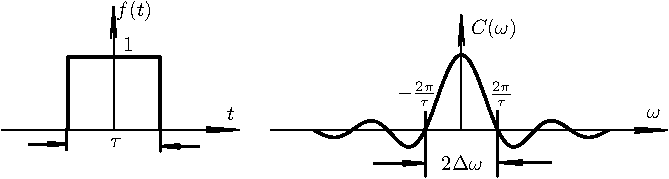
\includegraphics[width=0.6\linewidth]{Chapter_2/14}
	\caption{Биения при установлении колебаний
$(\Delta\omega\approx\gamma=\delta\omega/2)$}
	\figmark{fig10}
\end{figure}

Амплитуда колебаний при этом то растёт, то падает, причём максимумы амплитуд
постепенно уменьшаются. Лишь когда экспонента~$e^{-\gamma t}$ достаточно
затухнет, биения прекратятся, и колебания станут синусоидальными.
%\begin{center}
%СПИСОК ЛИТЕРАТУРЫ
%\end{center}

\introsection{Автоколебания}

\introsubsection{Автоколебания в системах с одной степенью свободы}
В предыдущих разделах были рассмотрены свободные и вынужденные колебания в
диссипативных системах с одной степенью свободы, подчиняющихся дифференциальным
уравнениям второго порядка вида \chaptereqref{2.8} и \chaptereqref{2.45}
соответственно. Диссипация энергии, обусловленная наличием резистивных элементов
в этих системах, в первом случае приводила к затуханию колебаний, а во
втором~--- компенсировалась энергией, поступающей от
внешнего источника синусоидального напряжения (или тока). Однако колебания в
системе с одной степенью свободы при определённых условиях можно поддерживать,
используя и \emph{постоянный} (не синусоидальный) источник энергии, 
который периодически компенсирует потери колебательной энергии по входящей 
в систему цепи \term{обратной связи}. 
Такие системы называются \term{автоколебательными}, а протекающие в
них процессы~--- \term{автоколебаниями}. Форма и период автоколебаний
определяются свойствами самой системы, чем автоколебания существенно отличаются
от обычных вынужденных колебаний

Для определения условий возбуждения автоколебаний в диссипативной системе с
одной степенью свободы воспользуемся уравнением изменения энергии 
системы \chaptereqref{JL}:
\begin{equation}
	\eqmark{auto-1}
	\frac{dW}{dt}=-P(t),
\end{equation}
где $W=\frac12 LI^2+ \frac{q^2}{2C}$~--- энергия, запасённая в колебательном контуре,
а $P(t)$~--- мощность потерь. 
Интегрируя \eqref{auto-1} по периоду колебаний $T$, приходим 
к равенству
\begin{equation}
	\eqmark{auto-2}
	W=W_0-\int\limits_{0}^{T}P(t)dt,
\end{equation}
где $W_0$~---~энергия системы в некоторый момент времени, принятый за начало
отсчёта. В обычной~--- диссипативной~--- системе $P(t)=RI^{2}(t)>0$, 
так что автоколебания невозможны. 
Если же мощность потерь $P(t)$ в системе можно сделать \important{знакопеременной}, 
то подбором режима работы системы можно обеспечить энергетический баланс:
\begin{equation}
	\eqmark{auto-3}
	\int\limits_{0}^{T} P(t) dt = 0,
\end{equation}
и, следовательно, возбудить в системе автоколебания. Отрицательные
<<потери>>, естественно, реализуются за счёт совершения 
работы внешним источником над системой.

Выполнение условия \eqref{auto-3} возможно, например, в \important{нелинейной}
колебательной системе, в которой сопротивление $R=\frac{dU}{dI}$ является 
функцией тока: $R=R(I)$, причём \emph{знакопеременной}. То есть для 
автоколебательного режима необходима возможность реализации
отрицательного \term{дифференциального сопротивления} цепи:
\[
R_{диф} = \frac{dU}{dI} < 0.
\]
Иными словами, вольт-амперная характеристика $I(U)$ элемента должна
обладать <<спадающими>> участками (участками с отрицательным наклоном). 
Примеры таких характеристик приведены на
рис.~\figref{auto-1}(а, б). Ими обладают, например, газоразрядная лампа 
(а) и туннельный диод (б). Обычно характеристики вида~(а) называют $S$-образными, 
а вида~(б)~---~$N$-образными.
\begin{figure}
	\centering
	\pic{0.8\textwidth}{Chapter_2/auto-1}
	%\import{Images/Chapter_2/}{auto-1.pdf_tex}
	\caption{Вольт-амперные характеристики с «падающими» участками: а)~$S$-образным, б) $N$-образным.}
	\figmark{auto-1}
\end{figure}

Форма автоколебаний зависит от добротности колебательного контура. При большой
добротности характер протекающих процессов почти не изменяется по сравнению с
тем, как они протекали бы в системе без поступления
энергии от источника: период и форма автоколебаний будут близки к периоду и
форме собственных колебаний. Это связано с тем, что в этом случае от постоянного
источника поступает энергия, составляющая малую
долю полной энергии колебательной системы. При малой добротности колебательной системы 
для поддержания колебаний от постоянного
источника должна поступать энергия, сопоставимая с энергией колебаний. В этом
случае форма автоколебаний может значительно отличаться от синусоидальной.
Наконец, в апериодической системе, в которой за период автоколебаний теряется вся
накопленная энергия, автоколебания становятся \term{релаксационными} и
могут по форме очень сильно отличаться от колебаний синусоидальных.

\introsubsection{Автоколебания в вырожденных системах}
Автоколебательная система, не содержащая одного из накопителей колебательной
энергии (например, индуктивности или емкости), называется \term{вырожденной}. Колебания в такой системе
описываются дифференциальным уравнением первого порядка и могут быть
только \emph{релаксационными}.

В качестве примера рассмотрим представленную на рис.~\figref{auto-2}(а,~б) 
вырожденную автоколебательную систему, содержащую источник
постоянного напряжения $U$, ёмкость $C$, сопротивление $R$ и нелинейный элемент
с $S$-образной вольт-амперной характеристикой $I_S(U)$. 

\begin{figure}[h]
	\begin{minipage}[h]{0.49\linewidth}
		\centering
		\pic{0.9\textwidth}{Chapter_2/auto-2}
		%\center{\resizebox{0.79\textwidth}{!}{\import{Images/Chapter_2/}{auto-2.pdf_tex}} \\ а) Схема автоколебательной $RC$-системы.}
	\end{minipage}
	\hfill
	\begin{minipage}[h]{0.49\linewidth}
		\centering
		\pic{0.79\textwidth}{Chapter_2/auto-3}
		%\center{\resizebox{0.79\textwidth}{!}{\import{Images/Chapter_2/}{auto-3.pdf_tex}} \\ б) Вольт-амперная характеристика и нагрузочная прямая $RC$-системы.}
	\end{minipage}
	\caption{Вырожденная автоколебательная $RC$-система}
	\figmark{auto-2}
\end{figure}

Уравнения, описывающие поведение этой системы релаксационного типа,
имеют вид:
\begin{equation}
	\eqmark{auto-4}
	RI+U=\mathcal{E},\quad I=I_C+I_S,\quad I_C=C\frac{dU}{dt},\quad I_S=I_S\left(U \right).
\end{equation}
Следовательно,
\begin{equation}
	\eqmark{auto-5}
	\tau_С\frac{dU}{dt}=\mathcal{E}-U-R{{I}_{S}}\left( U \right),
\end{equation}
где $\tau_С = RC$ --- характерное время разрядки конденсатора.

В стационарном состоянии, когда $dU / dt = 0$, должно выполняться равенство
\begin{equation}
	\eqmark{auto-6}
	I_S(U)=\frac{\mathcal{E}-U}{R}.
\end{equation}
Правая часть здесь представляет \important{нагрузочную прямую}, точки
пересечения которой с вольт-амперной характеристикой 
${I}_{S}\left( U \right)$ определяют стационарные состояния системы. 
На рис.~\figref{auto-2}б) параметры $\mathcal{E}$ и $R$ выбраны так, 
чтобы стационарное состояние $A(U_{А},\,I_{А})$ лежало на падающей
ветви вольт-амперной характеристики, где возможен автоколебательный режим. 

Покажем, что состояние $I_{А}=I(U_{А})$ может быть
\important{неустойчивым}. Для этого дадим малое приращение $\Delta U$ 
переменной $U$ в точке $U_{А}$ и представим в линейном приближении по 
$\delta U$ вольт-амперную характеристику $I_S(V)$ вблизи стационарного 
состояния $U_{А}$:
\begin{equation}
	\eqmark{auto-7}
I_S(U_{А} + \delta U)\approx 
    I_S(U_{А}) + {I}_S' \delta U,
\end{equation}
где ${I}_S' = \left.\frac{dI_S}{dU}\right|_{U_{А}}$ --- 
наклон вольт-амперной характеристики в точке~$U_{А}$. 
Подстановка этого выражения в \eqref{auto-5} приводит к уравнению
\begin{equation}
	\eqmark{auto-8}
\tau_С \frac{d\delta U}{dt}=-\left( 1+R{I}_S' \right) \delta U,
\end{equation}
из которого видно, что при условии
\begin{equation}
	\eqmark{auto-9}
	I_S' < - \frac{1}{R}
\end{equation}
возмущение $\delta U$ со временем экспоненциально нарастает, 
и, значит, стационарное состояние $I_{А}=I_S(U_{А})$ является неустойчивым. 

Если выполнено условие неустойчивости, система будет совершать
\important{релаксационные автоколебания}. 
Их фазовая траектория на рис.~\figref{auto-2}б) является замкнутой и 
состоит из плавных участков $da$ и $bc$ вольт-амперной
характеристики между напряжениями $U_1$ и $U_2$, соединённых двумя вертикальными
участками $ab$ и $cd$, показанными на рисунке штриховыми линиями. Формально
вертикальные участки соответствуют \important{скачкам тока}, которые возможны
только при отсутствии индуктивностей в системе, исходно заложенной в данной
идеализированной модели. Учёт малой «паразитной» индуктивности элементов схемы, 
приводящей к конечной скорости скачков, добавляет ещё одно дифференциальное 
уравнение первого порядка. Система, таким образом, перестаёт быть вырожденной, 
а в такой системе заведомо возможен автоколебательный процесс.

Аналогичным образом можно показать, что условие возбуждения автоколебаний 
в вырожденной $RL$-системе: соединённых последовательно с источником постоянного 
напряжения резистора, индуктивности и элемента с $N$-образной вольт-амперной 
характеристикой, --- имеет вид неравенства \eqref{auto-9}, 
в котором вместо $I_S'\left(U_{А}\right)$ стоит $I_N'\left(U_{А}\right)$ --- 
крутизна падающего  участка $N$-образной вольт-амперной характеристики 
в рабочей точке $\left(U_{А}\right)$.


\begin{lab:literature}
	\item~\emph{Сивухин~Д.В.} Общий курс физики.~Т.~III, Электричество.
\textbf{--} М.:~Физматлит, 2006, \S\S~122-124, 126, 127 129, 130.
	\item~\emph{Кингсеп~А.С., Локшин~Г.Р., Ольхов~О.А.} Основы физики.~Т.~I.
\textbf{--} М.:~Физматлит, 2001, \S\S~8.1-8.3.
	\item~\emph{Кириченко~Н.А.} Электричество и магнетизм. --- М.:~МФТИ,
2011. Гл.~17.
	\item~\emph{Горелик~Г.С. Колебания и волны.} --- М.:~Физматлит,
1959. Гл.~I, II, III.
	\item~\emph{Гоноровский~И.С.} Основы радиотехники. --- М.:~Связьиздат, 1957. Гл.~4.
\end{lab:literature}
\todo[inline,author=Popov]{Ссылки на учебники 50-х годов в издании 2018 выглядят
    странно. С тех пор лучших книг не выходило?}

\introsection{Автоколебания}

\introsubsection{Автоколебания в системах с одной степенью свободы}
В предыдущих разделах были рассмотрены свободные и вынужденные колебания в
диссипативных системах с одной степенью свободы, подчиняющихся дифференциальным
уравнениям второго порядка вида \chaptereqref{2.8} и \chaptereqref{2.45}
соответственно. Диссипация энергии, обусловленная наличием резистивных элементов
в этих системах, в первом случае приводила к затуханию колебаний, а во
втором~--- компенсировалась энергией, поступающей от
внешнего источника синусоидального напряжения (или тока). Однако колебания в
системе с одной степенью свободы при определённых условиях можно поддерживать,
используя и \emph{постоянный} (не синусоидальный) источник энергии, 
который периодически компенсирует потери колебательной энергии по входящей 
в систему цепи \term{обратной связи}. 
Такие системы называются \term{автоколебательными}, а протекающие в
них процессы~--- \term{автоколебаниями}. Форма и период автоколебаний
определяются свойствами самой системы, чем автоколебания существенно отличаются
от обычных вынужденных колебаний

Для определения условий возбуждения автоколебаний в диссипативной системе с
одной степенью свободы воспользуемся уравнением изменения энергии 
системы \chaptereqref{JL}:
\begin{equation}
	\eqmark{auto-1}
	\frac{dW}{dt}=-P(t),
\end{equation}
где $W=\frac12 LI^2+ \frac{q^2}{2C}$~--- энергия, запасённая в колебательном контуре,
а $P(t)$~--- мощность потерь. 
Интегрируя \eqref{auto-1} по периоду колебаний $T$, приходим 
к равенству
\begin{equation}
	\eqmark{auto-2}
	W=W_0-\int\limits_{0}^{T}P(t)dt,
\end{equation}
где $W_0$~---~энергия системы в некоторый момент времени, принятый за начало
отсчёта. В обычной~--- диссипативной~--- системе $P(t)=RI^{2}(t)>0$, 
так что автоколебания невозможны. 
Если же мощность потерь $P(t)$ в системе можно сделать \important{знакопеременной}, 
то подбором режима работы системы можно обеспечить энергетический баланс:
\begin{equation}
	\eqmark{auto-3}
	\int\limits_{0}^{T} P(t) dt = 0,
\end{equation}
и, следовательно, возбудить в системе автоколебания. Отрицательные
<<потери>>, естественно, реализуются за счёт совершения 
работы внешним источником над системой.

Выполнение условия \eqref{auto-3} возможно, например, в \important{нелинейной}
колебательной системе, в которой сопротивление $R=\frac{dU}{dI}$ является 
функцией тока: $R=R(I)$, причём \emph{знакопеременной}. То есть для 
автоколебательного режима необходима возможность реализации
отрицательного \term{дифференциального сопротивления} цепи:
\[
R_{диф} = \frac{dU}{dI} < 0.
\]
Иными словами, вольт-амперная характеристика $I(U)$ элемента должна
обладать <<спадающими>> участками (участками с отрицательным наклоном). 
Примеры таких характеристик приведены на
рис.~\figref{auto-1}(а, б). Ими обладают, например, газоразрядная лампа 
(а) и туннельный диод (б). Обычно характеристики вида~(а) называют $S$-образными, 
а вида~(б)~---~$N$-образными.
\begin{figure}
	\centering
	\pic{0.8\textwidth}{Chapter_2/auto-1}
	%\import{Images/Chapter_2/}{auto-1.pdf_tex}
	\caption{Вольт-амперные характеристики с «падающими» участками: а)~$S$-образным, б) $N$-образным.}
	\figmark{auto-1}
\end{figure}

Форма автоколебаний зависит от добротности колебательного контура. При большой
добротности характер протекающих процессов почти не изменяется по сравнению с
тем, как они протекали бы в системе без поступления
энергии от источника: период и форма автоколебаний будут близки к периоду и
форме собственных колебаний. Это связано с тем, что в этом случае от постоянного
источника поступает энергия, составляющая малую
долю полной энергии колебательной системы. При малой добротности колебательной системы 
для поддержания колебаний от постоянного
источника должна поступать энергия, сопоставимая с энергией колебаний. В этом
случае форма автоколебаний может значительно отличаться от синусоидальной.
Наконец, в апериодической системе, в которой за период автоколебаний теряется вся
накопленная энергия, автоколебания становятся \term{релаксационными} и
могут по форме очень сильно отличаться от колебаний синусоидальных.

\introsubsection{Автоколебания в вырожденных системах}
Автоколебательная система, не содержащая одного из накопителей колебательной
энергии (например, индуктивности или емкости), называется \term{вырожденной}. Колебания в такой системе
описываются дифференциальным уравнением первого порядка и могут быть
только \emph{релаксационными}.

В качестве примера рассмотрим представленную на рис.~\figref{auto-2}(а,~б) 
вырожденную автоколебательную систему, содержащую источник
постоянного напряжения $U$, ёмкость $C$, сопротивление $R$ и нелинейный элемент
с $S$-образной вольт-амперной характеристикой $I_S(U)$. 

\begin{figure}[h]
	\begin{minipage}[h]{0.49\linewidth}
		\centering
		\pic{0.9\textwidth}{Chapter_2/auto-2}
		%\center{\resizebox{0.79\textwidth}{!}{\import{Images/Chapter_2/}{auto-2.pdf_tex}} \\ а) Схема автоколебательной $RC$-системы.}
	\end{minipage}
	\hfill
	\begin{minipage}[h]{0.49\linewidth}
		\centering
		\pic{0.79\textwidth}{Chapter_2/auto-3}
		%\center{\resizebox{0.79\textwidth}{!}{\import{Images/Chapter_2/}{auto-3.pdf_tex}} \\ б) Вольт-амперная характеристика и нагрузочная прямая $RC$-системы.}
	\end{minipage}
	\caption{Вырожденная автоколебательная $RC$-система}
	\figmark{auto-2}
\end{figure}

Уравнения, описывающие поведение этой системы релаксационного типа,
имеют вид:
\begin{equation}
	\eqmark{auto-4}
	RI+U=\mathcal{E},\quad I=I_C+I_S,\quad I_C=C\frac{dU}{dt},\quad I_S=I_S\left(U \right).
\end{equation}
Следовательно,
\begin{equation}
	\eqmark{auto-5}
	\tau_С\frac{dU}{dt}=\mathcal{E}-U-R{{I}_{S}}\left( U \right),
\end{equation}
где $\tau_С = RC$ --- характерное время разрядки конденсатора.

В стационарном состоянии, когда $dU / dt = 0$, должно выполняться равенство
\begin{equation}
	\eqmark{auto-6}
	I_S(U)=\frac{\mathcal{E}-U}{R}.
\end{equation}
Правая часть здесь представляет \important{нагрузочную прямую}, точки
пересечения которой с вольт-амперной характеристикой 
${I}_{S}\left( U \right)$ определяют стационарные состояния системы. 
На рис.~\figref{auto-2}б) параметры $\mathcal{E}$ и $R$ выбраны так, 
чтобы стационарное состояние $A(U_{А},\,I_{А})$ лежало на падающей
ветви вольт-амперной характеристики, где возможен автоколебательный режим. 

Покажем, что состояние $I_{А}=I(U_{А})$ может быть
\important{неустойчивым}. Для этого дадим малое приращение $\Delta U$ 
переменной $U$ в точке $U_{А}$ и представим в линейном приближении по 
$\delta U$ вольт-амперную характеристику $I_S(V)$ вблизи стационарного 
состояния $U_{А}$:
\begin{equation}
	\eqmark{auto-7}
I_S(U_{А} + \delta U)\approx 
    I_S(U_{А}) + {I}_S' \delta U,
\end{equation}
где ${I}_S' = \left.\frac{dI_S}{dU}\right|_{U_{А}}$ --- 
наклон вольт-амперной характеристики в точке~$U_{А}$. 
Подстановка этого выражения в \eqref{auto-5} приводит к уравнению
\begin{equation}
	\eqmark{auto-8}
\tau_С \frac{d\delta U}{dt}=-\left( 1+R{I}_S' \right) \delta U,
\end{equation}
из которого видно, что при условии
\begin{equation}
	\eqmark{auto-9}
	I_S' < - \frac{1}{R}
\end{equation}
возмущение $\delta U$ со временем экспоненциально нарастает, 
и, значит, стационарное состояние $I_{А}=I_S(U_{А})$ является неустойчивым. 

Если выполнено условие неустойчивости, система будет совершать
\important{релаксационные автоколебания}. 
Их фазовая траектория на рис.~\figref{auto-2}б) является замкнутой и 
состоит из плавных участков $da$ и $bc$ вольт-амперной
характеристики между напряжениями $U_1$ и $U_2$, соединённых двумя вертикальными
участками $ab$ и $cd$, показанными на рисунке штриховыми линиями. Формально
вертикальные участки соответствуют \important{скачкам тока}, которые возможны
только при отсутствии индуктивностей в системе, исходно заложенной в данной
идеализированной модели. Учёт малой «паразитной» индуктивности элементов схемы, 
приводящей к конечной скорости скачков, добавляет ещё одно дифференциальное 
уравнение первого порядка. Система, таким образом, перестаёт быть вырожденной, 
а в такой системе заведомо возможен автоколебательный процесс.

Аналогичным образом можно показать, что условие возбуждения автоколебаний 
в вырожденной $RL$-системе: соединённых последовательно с источником постоянного 
напряжения резистора, индуктивности и элемента с $N$-образной вольт-амперной 
характеристикой, --- имеет вид неравенства \eqref{auto-9}, 
в котором вместо $I_S'\left(U_{А}\right)$ стоит $I_N'\left(U_{А}\right)$ --- 
крутизна падающего  участка $N$-образной вольт-амперной характеристики 
в рабочей точке $\left(U_{А}\right)$.

\lab{Резонанс напряжений в последовательном контуре}
\label{lab:322}

\begin{lab:aim}
исследование резонанса напряжений в последовательном колебательном контуре
с изменяемой ёмкостью, получение амплитудно-частотных и
фазово-частотных характеристик, определение основных параметров контура.
\end{lab:aim}

\begin{lab:equipment}
	генератор сигналов, источник напряжения, нагрузкой которого является
последовательный колебательный контур с переменной ёмкостью, двухканальный
осциллограф, цифровые вольтметры.
\end{lab:equipment}

%\begin{lab:warning}
% \warning{
Перед выполнением работы необходимо ознакомиться с основами теории электрических  
колебаний (см. Введение пп. \ref{sec:forced}, \ref{sec:ures}).
Необходимые  дополнения применительно к реальным элементам колебательного
контура будут приведены ниже.
%по вводной части Раздела II настоящего сборника и/или рекомендованной в нём
%литературе. 
% }
%\end{lab:warning}

\experiment

В данной работе изучаются резонансные явления в последовательном колебательном
контуре (резонанс напряжений). 
Схема экспериментального стенда показана на рис.~\figref{exp}.
Синусоидальный сигнал от генератора поступает на вход \important{управляемого
напряжением источника напряжения} (см., напр., [3]), собранного на
операционном усилителе, питание которого осуществляется встроенным
блоком-выпрямителем от сети~$\sim220$~В (цепь питания на схеме не показана).
\emph{Источник напряжения} (источник с нулевым внутренним
сопротивлением) обеспечивает с высокой точностью постоянство
амплитуды сигнала~$\mathcal{E}=\mathcal{E}_0\cos(\omega t+\varphi_0)$ на
меняющейся по величине нагрузке~--- последовательном колебательном контуре,
изображенном на рис.~\figref{exp} в виде эквивалентной схемы. 

\begin{figure}[h!]
    \centering
	\pic{0.75\textwidth}{Chapter_2/2_2_2}
	\caption{Схема экспериментального стенда}
	\figmark{exp}
\end{figure}

Источник
напряжения, колебательный контур и блок питания заключены в отдельный корпус,
% с названием <<Резонанс напряжений>>, 
отмеченный на рисунке штриховой линией.
На корпусе имеются коаксиальные разъёмы <<Вход>>, <<$U_1$>> и <<$U_2$>>, а также
переключатель магазина ёмкостей $C_n$ с указателем номера $n=1,~2,~\ldots~7.$
Величины ёмкостей~$C_n$ указаны на установке. 
Напряжение~$\mathcal{E}$ на контуре через разъём <<$U_1$>> попадает одновременно 
на канал~1 осциллографа и вход 1-го цифрового вольтметра. Напряжение на конденсаторе~$U_C$ 
подаётся через разъём <<$U_2$>> одновременно на канал~2 осциллографа и
вход 2-го цифрового вольтметра.

\paragraph{Особенности реальных элементов цепи}
\label{par:real_elements}

Колебательный контур нашей установки собран из стандартных элементов,
используемых в современных радиоэлектронных цепях. Известно, что в реальных
конденсаторах и, особенно, в катушках индуктивности происходят 
\emph{необратимые потери} энергии, обусловленные различными причинами. К ним относятся: утечки и
диэлектрические потери в конденсаторах, вихревые токи и потери на
перемагничивание в сердечниках катушек индуктивности, омические потери в
проводниках, растущие с частотой за счёт скин-эффекта, и др. Рост
потерь приводит к увеличению действительных частей комплексных сопротивлений
элементов контура, и, значит, к изменению его резонансных свойств, в частности,
к уменьшению добротности~$Q$.

Потери в элементах контура зависят как от частоты, так и от амплитуды тока
(напряжения), температуры и ряда других факторов, например, от вида диэлектрика
конденсатора, сердечника катушки и т.\,д. От перечисленных факторов в общем случае
зависят и основные параметры контура: индуктивность $L,$ ёмкость $C$ и суммарное
активное сопротивление~$R_{\Sigma}$.

В нашем контуре катушка индуктивности $L$ на ферритовом каркасе обладает малым
сопротивлением по постоянному току и высокой собственной резонансной
частотой~$\nu_{L0}\ge1,3$~МГц. В общем случае каждая катушка, помимо индуктивности~$L,$ характеризуется также собственной (межвитковой) ёмкостью $C_L$ и активным
сопротивлением потерь~$R_L,$ распределёнными по её длине. Принимается, что эти
величины сосредоточены в отдельных элементах схемы, образующих с индуктивностью~$L$ 
замкнутую колебательную цепь с собственной резонансной частотой
$\nu_{L0}=1/2\pi\sqrt{LC_L}.$ Вследствие влияния ёмкости~$C_L$ при измерении на
частоте~$\nu$ определяется не истинная индуктивность~$L,$ а эффективное значение
индуктивности $L_{эфф}=L/(1-\nu^2/\nu_0^2),$ которое может заметно отличаться от
истинной величины~$L.$ В рабочем диапазоне частот нашего контура выполняется
неравенство $\nu \ll \nu_0,$ так что в эквивалентной схеме контура на рис.~\figref{exp}
индуктивность представлена своим истинным значением~$L$ и активным
сопротивлением~$R_L.$

\begin{figure}[h!]
    \centering\small
    \pic{0.65\textwidth}{Chapter_2/2_2_3}
    \caption{Последовательная эквивалентная схема конденсатора с потерями.}
    \figmark{equiv capacitor}
\end{figure}

Полипропиленовые конденсаторы с ёмкостями $C_n$ ($n=1\ldots7$), 
входящие в комплект магазина ёмкостей, в рабочем диапазоне частот имеют 
пренебрежимо малые собственные индуктивности (менее $10^{-5}$~мГн на 1~см общей длины обкладок и
выводов) и относительно малые активные потери. Для оценки возможного вклада
активных потерь в конденсаторах в общий импеданс контура воспользуемся
представлением конденсатора с ёмкостью~$C$ последовательной эквивалентной
схемой, показанной на рис.~\figref{equiv capacitor}а.
%\todo[author=Tiffani]{Нет рис 15 из ворд-файла в формате pic, проверить!}
На этой схеме $R_S$~---~так называемое \emph{эквивалентное последовательное
сопротивление} (ЭПС), обусловленное, главным образом, электрическим
сопротивлением материала обкладок и выводов конденсатора и контактов между ними,
а также потерями в диэлектрике. Из эквивалентной схемы и векторной диаграммы к
ней (рис.~\figref{equiv capacitor}б) видно, что активные потери в конденсаторе,
пропорциональные косинусу угла~$\varphi$ сдвига фаз между током и
напряжением на ёмкости, убывают с ростом~$\varphi$ и, соответственно, с
уменьшением угла $\delta=\frac{\pi}{2}-\varphi$. Потери в конденсаторе принято
характеризовать величиной $\tg\delta$, обычно приводимой в документации к
изделию. Из рис.~\figref{equiv capacitor} и закона Ома получаем 
выражение для ЭПС на циклической частоте $\omega=2\pi \nu$ в виде
\begin{equation}\eqmark{2.2.1}
R_S=\dfrac{U_{RS}}{I}=\dfrac{U_{RS}}{\omega CU_{CS}}=\dfrac{\tg\delta}{\omega C}.
\end{equation}
Конденсаторы магазина ёмкостей~$C_n$ в интересующем нас диапазоне частот имеют
$\tg\delta<10^{-3},$ что является очень хорошим (низким!) показателем для
конденсаторов с твёрдым диэлектриком.

\paragraph{Свойства колебательного контура}

В колебательный контур наших установок добавлен постоянный резистор $R$ (см.
рис.~\figref{exp}), снижающий его добротность. Это сделано для упрощения
процедур получения и обработки резонансных кривых. Таким образом, суммарное
активное сопротивление контура принимается равным
\begin{equation}\eqmark{2.2.2}
	R_{\Sigma}=R+R_L+R_S.
\end{equation}
Добротность контуров, тем не менее, остаётся достаточно высокой, чтобы можно
было пользоваться формулами \chaptereqref{2.35}, в которых
надо учитывать суммарное активное сопротивление контура:
\begin{equation}\eqmark{2.2.3}
	Q=\frac{\rho}{R_{\Sigma}}=\frac{\omega_0L}{R_{\Sigma}}=
    \frac{1}{\omega_0CR_{\Sigma}}\gg 1.
\end{equation}
Сильное неравенство в \eqref{2.2.3} в рабочем диапазоне частот выполняется для
всех контуров, используемых в работе.

Для импедансов ёмкости $Z_C$, индуктивности $Z_L$ и последовательного контура
$Z=Z_L+R+Z_C$ с учётом \eqref{2.2.1}, \eqref{2.2.2} получаем выражения:
\begin{equation}\eqmark{2.2.4}
Z_C=R_S-\dfrac{i}{\omega C}, \qquad Z_L=R_L+i\omega L,\qquad
Z=R_{\Sigma}+i\left(\omega L-\dfrac{1}{\omega C}\right).
\end{equation}
Комплексные амплитуды тока в контуре~$\vec I=\vec E/Z$ и напряжений
на сопротивлении~$\vec{U}_{\! R}=R\vec I,$ ёмкости $\vec{U}_{\! C}=Z_C\vec I$ и
индуктивности $\vec{U}_{\! L}=Z_L\vec I$ при нулевой начальной фазе $\varphi_0$
напряжения на контуре $\vec{\mathcal{E}}=\mathcal{E}_0e^{i\varphi_0}$ 
по формулам~\chaptereqref{2.48a}, \chaptereqref{2.48b} 
с учётом \eqref{2.2.1}--\eqref{2.2.4} удобно записать в виде
%\begin{subequations}
%	\eqmark{2.2.5}
		\begin{equation}
			\eqmark{2.2.5a}
			\vec I=\dfrac{\vec
U_R}{R}=\dfrac{\mathcal{E}_0}{R_{\Sigma}}\dfrac{1}{
1+iQ(\omega/\omega_0-\omega_0/\omega)}, \end{equation}
		\begin{equation}
			\eqmark{2.2.5b}
			\vec
U_C=-iQ\mathcal{E}_0\dfrac{\omega_0}{\omega}\dfrac{1+i\tg\delta}{
1+iQ(\omega/\omega_0-\omega_0/\omega)},
		\end{equation}
		\begin{equation}
			\eqmark{2.2.5c}
			\vec
U_L=iQ\mathcal{E}_0\dfrac{\omega}{\omega_0}\dfrac{1-iR_L/\rho}{
1+iQ(\omega/\omega_0-\omega_0/\omega)}.
		\end{equation}
%\end{subequations}
Эти формулы уточняют результаты \chaptereqref{2.48a}--\chaptereqref{2.48b} и 
\chaptereqref{2.54a}--\chaptereqref{2.54d},
полученные без учёта потерь в конденсаторе и в катушке индуктивности. Отметим,
однако, что указанными потерями, представленными мнимыми добавками в числителях
формул~\eqref{2.2.5b} и~\eqref{2.2.5c}, при условиях $Q\gg1$ и
$\tg \delta \gg 10^{-3}$ можно пренебречь. В~то же время вклад этих потерь в
суммарное активное сопротивление контура $R_{\Sigma}$, вблизи
резонанса составляющий приблизительно $R_L+\rho\tg\delta$, 
можно оценить только по результатам эксперимента.

Основные особенности резонанса в последовательном контуре, называемого также
\important{резонансом напряжений} из-за увеличения в $Q$ раз напряжений на
ёмкости $U_C$ и индуктивности $U_L$ по отношению к внешнему напряжению
$\mathcal{E}_0,$ следуют из анализа формул \eqref{2.2.5a}--\eqref{2.2.5c}. 
Подробно этот вопрос рассматривался в п.~\ref{sec:ures} Введения к разделу.
%\todo[author=Tiffani]{уточнить номер пункта (п.~3.1?)}

Наибольший практический интерес представляет случай, когда отклонение
$\delta\omega=\omega-\omega_0$ частоты внешней ЭДС от собственной частоты
контура $\omega_0$ удовлетворяет сильному неравенству
%\setcounter{equation}{5}
\begin{equation}\eqmark{2.2.6}
	|\Delta\omega| \ll \omega_0.
\end{equation}
При этом в первом порядке малости по относительной расстройке частоты
$\Delta\omega/\omega_0$
\begin{equation}\eqmark{2.2.7}
\dfrac{\omega}{\omega_0}-\dfrac{\omega_0}{\omega}=
\dfrac{2\Delta\omega}{\omega_0},
\end{equation}
что позволяет упростить выражения \eqref{2.2.5a}--\eqref{2.2.5c},
и представить вещественные части комплексных амплитуд 
и соответствующих им фаз в виде:
\begin{align}
%	\eqmark{2.2.8}
%		\begin{equation}
			\eqmark{2.2.8a}
    	I & =\dfrac{U_R}{R}=\dfrac{\mathcal{E}_0}{R_{\Sigma}}
            \dfrac{\cos(\omega t-\psi_I)}{\sqrt{1+(\tau\Delta\omega)^2}}, &
        \psi_I &= \arctg (\tau\Delta\omega), \\
%		\end{equation}
%		\begin{equation}
			\eqmark{2.2.8b}
		U_C &= Q\mathcal{E}_0\dfrac{\omega_0}{\omega}
            \dfrac{\cos(\omega t-\psi_C)}{\sqrt{1+(\tau\Delta\omega)^2}}, &
        \psi_C &= \psi_I +\dfrac{\pi}{2}-\delta, \\
%		\end{equation}
%		\begin{equation}
			\eqmark{2.2.8c}
			U_L & =Q\mathcal{E}_0\dfrac{\omega}{\omega_0}
                \dfrac{\cos(\omega t-\psi_L)}{\sqrt{1+(\tau\Delta\omega)^2}}, &
        \psi_L & = \psi_I -\dfrac{\pi}{2}+\dfrac{R_L}{\rho}.
%		\end{equation}
\end{align}
Здесь $\tau$ --- время затухания \chaptereqref{2.24}. В выражениях \eqref{2.2.8b}, \eqref{2.2.8c} мы сохранили в прежнем виде
множители с отношениями частот в амплитудах и учли только линейные по малым
величинам $R_L/\rho$ и $\delta$ поправки в фазах, причём величину $\delta$
сохранили исключительно для общности, положив её константой.

При резонансе, когда для высокодобротного контура можно положить 
$\omega=\omega_0$ ($\Delta\omega=0$), 
выражения для модулей комплексных амплитуд тока и напряжения на ёмкости, 
и их фаз принимают вид (ср. \chaptereqref{2.61}):
%и производных фаз по частоте $\omega$ принимают вид:
\begin{align}
%	\eqmark{2.2.9}
%		\begin{equation}
			\eqmark{2.2.9a}
		I(\omega_0) & =\dfrac{U_R}{R}=\dfrac{\mathcal{E}_0}{R_{\Sigma}}, &
        \varphi_I(\omega_0) & = 0, \\
%		\end{equation}
%		\begin{equation}
			\eqmark{2.2.9b}
		U_C(\omega_0) & = Q\mathcal{E}_0, &
            \psi_C(\omega_0) & = \dfrac{\pi}{2}-\delta; \\
        U_L(\omega_0) & = Q\mathcal{E}_0, &
            \psi_L(\omega_0) &=-\dfrac{\pi}{2}+\dfrac{R_L}{\rho}.
%		\end{equation}
%		\begin{equation}
%			\eqmark{2.2.9c}
%			\psi_I'(\omega_0)=\psi_C'(\omega_0)=\psi_L(\omega_0)=\tau.
%		\end{equation}
\end{align}
%Из формул \eqref{2.2.8}, \eqref{2.2.9} 
Из полученных соотношений следует, что на частоте $\omega_0,$ где
импеданс контура $Z$ становится чисто активным и равным $R_{\Sigma},$ амплитуда
тока достигает максимального значения $I_{\rm max}=\mathcal{E}_0/R_{\Sigma}.$
Напряжения $U_L$ и $U_C$ на индуктивности и ёмкости на частоте $\omega_0$
находятся почти в противофазе и в~$Q$ раз превышают по амплитуде напряжение
$\mathcal{E}$ внешней ЭДС. Напомним, однако, что максимальные (резонансные)
значения напряжений на индуктивности и ёмкости не
строго равны $Q\mathcal{E}_0$ и достигаются не строго на частоте $\omega_0$.
Соответствующие поправки, обусловленные множителями
$(\omega_0/\omega)^{\pm1}$ в амплитудах и малыми добавками к фазам в выражениях
для $U_C$ \eqref{2.2.8b} и $U_L$ \eqref{2.2.8c}, 
имеют порядок малости~$Q^{-2}$.
%\todo[author=Tiffani]{уточнить номер пункта (п.~3.1?)}

При отклонении $\Delta\omega$ частоты внешней ЭДС от $\omega_0$ таком, что
выполняется условие
%\setcounter{equation}{9}
\begin{equation}\eqmark{2.2.10}
\tau\Delta\omega=\pm1,
\end{equation}
амплитуда тока $I,$ как видно из \eqref{2.2.8a}, уменьшается в $\sqrt{2}$
раз относительно своей максимальной (резонансной) величины, а фаза $\psi_I$
изменяется на угол $\pm\pi/4$. 
В этой же точке, если не учитывать
поправки порядка $Q^{-1},$ происходят аналогичные изменения
амплитуд $U_C$, $U_L$ и фаз $\psi_C,~\psi_L$ напряжений на ёмкости и
индуктивности: амплитуды уменьшаются в $\sqrt{2}$ раз, а фазы меняются на угол
$\pm\pi/4$ по отношению к своим резонансным значениям.

Величина $\delta\omega=2|\Delta\omega|=2/\tau$ представляет собой важную
характеристику колебательного контура~--- \emph{ширину резонансной кривой}~$U_C(\omega)$
на уровне $U_C(\omega_0)/\sqrt{2}$, по которой можно определить
время затухания $\tau=2/\delta\omega$ и, зная резонансную частоту~$\omega_0$,
найти добротность контура $Q=\omega_0/\delta\omega$.

Эти же параметры можно определить по фазово-частотной характеристике: расстояние
по оси $\omega$ между точками, в которых фаза $\varphi_C$ меняется от $-\pi/4$
до $3\pi/4,$ согласно \eqref{2.2.8b} равно $2/\tau,$ а тангенс угла наклона
функции $\varphi_C(\omega)$ в точке резонанса согласно \chaptereqref{2.61c} определяет
время затухания~$\tau$.

В нашем эксперименте резонансные явления в последовательном колебательном
контуре исследуются по напряжению на контуре $\mathcal{E}$ и напряжению на
ёмкости $U_C$ (см. рис.~\figref{exp}), а также по фазовым сдвигам между ними.
%Приведённые выше формулы для других характеристик дополняют общую картину
%рассматриваемых процессов. В частности, они могут быть использованы для
%построения векторных диаграмм.

\begin{lab:task}

\item Проведите настройку экспериментального стенда по техническому описанию установки.
В двухканальном режиме работы осциллографа установите общее начало отсчёта $Y_1(t)$, $Y_2(t)$ вблизи левого края
средней линии экрана. В качестве синхронизующего сигнала выберите напряжение
$\mathcal{E}(t)$ при начальных условиях: $\mathcal{E}(0)=0,
\dot{\mathcal{E}}(0)<0.$

\item Установите на выходе генератора (на входе схемы) эффективное 
значение напряжения $\mathcal{E}$, указанное преподавателем 
(в пределах $30\div300$~мВ). Меняя частоту $\nu=\omega/2\pi$ генератора, 
убедитесь по осциллографу и вольтметрам, что у синусоиды $U_C(t)$ меняется амплитуда и фаза
относительно начала координат, тогда как синусоида
$\mathcal{E}(t)$~--- синхронизующий сигнал~--- <<привязана>> к началу отсчёта
при начальных условиях: $\mathcal{E}(0)=0, \dot{\mathcal{E}}(0)<0$~---~а её
амплитуда~$\mathcal{E}_0$ остаётся неизменной с относительной погрешностью не
менее $1\%$. 

\item Для контуров с 7 различными ёмкостями $C_n$, меняя их с помощью
переключателя на блоке, измерьте резонансные частоты $\nu_{0n}$ и напряжения
$U_C(\nu_{0n})$ при установленном в п.~2 напряжении~$\mathcal{E}$ на выходе
генератора. Регистрируйте также напряжения $\mathcal{E}(\nu_{0n})$, игнорируя
отклонения в пределах относительной погрешности~$1\%$. Приближение к резонансу
удобно наблюдать по фигуре Лиссажу на экране осциллографа в режиме $X$--$Y$.
При этом фигура Лиссажу представляет собой эллипс, оси которого на собственной
частоте~$\nu_{0n}$ направлены по~$X$ и~$Y$. 
Напомним, что максимальные значения напряжения~$U_C(\nu)$ достигаются на частотах, 
несколько отличных от собственных частот~$\nu_{0n}$.

    \item \footnote{Дополнительное упражнение, выполняется по указанию
        преподавателя.}Проделайте измерения п.~3 ещё
для двух напряжений $\mathcal{E}$ из интервала $30\div 300~мВ,$ существенно
отличающихся друг от друга и от напряжения, использованного в п.~3.

    \item Для контуров с двумя разными ёмкостями (по указанию преподавателя)
измерьте амплитудно-частотные характеристики $U_C(\nu)$ для значений
$U_C(\nu) \ge 0,6 U_C(\nu_{0n})$ (всего 16--18 точек по обе стороны от резонанса)
при том же напряжении~$\mathcal{E}$, что и в п.~3.

    \item Для тех же двух контуров измерьте фазово-частотные характеристики
$\psi_C(\nu)$ для значений $U_C(\nu)\ge0,3U_C(\nu_{0n})$ (всего 16--18 точек по
обе стороны от резонанса) при том же напряжении~$\mathcal{E},$ что и в п.~3.

Перед выполнением этого задания проверьте настройки осциллографа:
синхронизующий сигнал~$\mathcal{E}(t),$ как указано в п.~2, должен был
<<привязан>> к общему началу отсчёта времени и напряжений на экране, лежащему на
оси~$X$ координатной сетки экрана. На той же оси должны располагаться нули
сигналов~$\mathcal{E}(t)$ и~$U_C(t)$. Если это не так, то следует повторить
процедуру центрирования горизонтальных осей каналов по техническому описанию.

Расстояние $x$ от начала отсчёта до точки первого обращения в нуль
напряжения $U_C(t)$ на участке спада характеризует разность фаз $\Delta\varphi$
сигналов $\mathcal{E}(t)$ и $U_C(t)$. Эта величина, выраженная в радианах,
даётся формулой $\Delta\varphi=\frac{x}{x_0}\pi$, где $x_0$~--- расстояние
от начала отсчёта до точки первого обращения в нуль напряжения $\mathcal{E}(t)$
на участке подъёма, соответствующее полупериоду этого сигнала.

\tasksection{Обработка и представление результатов}

% 		    \important{Настоятельно рекомендуется для обработки и представления
% результатов измерений использовать электронные таблицы.}

		    \item Результаты измерений п.~3 внесите в таблицу:\par
%		    \begin{center}
%		        \begin{table}[tb!]
		           % \caption{\eqmark{tab:1}
%		            \caption{}
%		            \tabmark{2.2.1}
%		            \begin{center}
\begingroup\small
\noindent\begin{tabular}{|c|c|c|c|c|c|c|c|c|c|c|} 
		                    \hline
		                    $C_n,$ & $f_{0n},$& $U_C,$& $\mathcal{E},$ & $L,$~&
$Q$& $\rho,$ & $R_{\Sigma},$~& $R_{S\text{max}},$& $R_L,$& $I,$\\

		                    нФ & кГц & В & В & мкГн &  & Ом & Ом & Ом & Ом & мА
\\
		                    \hline
		                    $C_1$ & & & & & & & & & & \\
		                    \hline
		                    $\cdots$ &  & & &  &  &  &  & & & \\
		                    \hline
		                    $C_7$& & & & & & & & & & \\
		                    \hline
		                    \multicolumn{4}{|c|}{Среднее значение} & & & & & & & \\
		                    \hline
		                    \multicolumn{4}{|c|}{Среднекв. отклонение} & & & & & & & \\ \hline
%		                    \multicolumn{4}{|c|}{Коэфф. Стьюдента} & & & & & & & \\
%		                    \multicolumn{4}{|c|}{$t_{n\alpha}$, $n=7$, $\alpha=0,05$} &
%& & & & & & \\ \hline
%		                    \multicolumn{4}{|c|}{для~$n=7,~\alpha=0,95$} &  & &
%& & && \\
%		                    \hline
%%		                    \multicolumn{4}{|c|}{ Коэффициент Стьюдента
%% $t_{n\alpha}$~для~$n=7,~\alpha=0,95$} & ---& & & & &---&\\
%%		                    \hline
%		                    \multicolumn{4}{|c|}{ Случайная погрешность } & ---&
%& & & &---&\\
%
		                    \multicolumn{4}{|c|}{Случ. погрешность} & & & & & & & \\ \hline
%		                    \hline
		                \end{tabular}
%		            \end{center}
%		        \end{table}
%		    \end{center}
\endgroup%\small

В первый столбец запишите значения ёмкостей~$C_n$,
приведённые в табличке на корпусе блока <<Резонанс напряжений>>. Для каждого
значения $C_n$ по формулам вводной части и данным эксперимента проведите
последовательно расчёт $L$, $Q$, $\rho$, $R_{\Sigma}$,
$R_{S\text{max}}=10^{-3}\rho$, $R_L$, $I$. Затем рассчитайте
средние значения $\left< L \right>$ и $\left< R_L \right>$ 
и их случайные погрешности ~$\Delta L$ и~$\Delta R_L$.

%Представьте результат проделанных в работе \important{косвенных
%измерений при невоспроизводимых условиях} величин $L$ и $R_L$ в виде: $\langle
%L\rangle\pm\Delta L$ и $\langle R_L\rangle\pm\Delta R_L,$ где угловыми скобками
%отмечены средние значения, а символом <<$\Delta$>>~--- случайные погрешности
%величин~$L$ и~$R_L$.

Оцените относительный вклад активных потерь в конденсаторах
(представленных в таблице сопротивлением $R_{S\text{max}}$, рассчитанным
для максимального значения $\tg\delta=10^{-3}$) в суммарное активное
сопротивление контура. Оцените влияние погрешностей приборов на результаты
измерений.

    \item *Выполните задание п.~7 для данных, полученных в п.~4. 
    Сравните с результатами п.~7. Объясните причины расхождения результатов, 
    если они обнаружатся.

    \item По данным измерений п.~5 постройте на одном графике
амплитудно-частотные характеристики $U_C(\nu)$ для выбранных
контуров. Проведите сравнительный анализ характеристик.

    \item По данным измерений п.~5 постройте на одном графике
амплитудно-частотные характеристики в безразмерных координатах 
$x\equiv \nu/\nu_{0n}$, $y\equiv U_C(x)/U_C(1)$. 
По ширине резонансных кривых на уровне $0,707$ определите добротности $Q$ 
соответствующих контуров. Оцените погрешности. 
Сравните эти величины с данными п.~7.

    \item По данным измерений п.~6 постройте на одном графике
фазово-частотные характеристики в координатах 
$x\equiv \nu/\nu_{0n}$, $y\equiv\varphi_C/\pi$ для выбранных контуров. 
По этим характеристикам определите
добротности контуров одним из двух способов: по расстоянию между точками по оси~$x$, 
в которых $y$ меняется от $1/4$ до $3/4$, равному $1/Q$, или по формуле
$Q=0,5\frac{d\varphi_C}{dx}$ при $x=0$. Оцените погрешности. 
Сравните с результатами пп.~7,~10.

    \item Постройте зависимость $R_L(\nu_{0n})$ в системе координат с началом 
    в точке $(0,6\nu_{07};0);$ нанесите на график прямую $\langle R_L\rangle$. 
    Назовите возможные причины изменения $R_L$ с частотой.

    \item Постройте векторную диаграмму тока и напряжений для контура 
    с наименьшей добротностью в резонансном состоянии. Ось абсцисс направьте 
    по вектору $\vec{\mathcal{E}}$.

\end{lab:task}


\begin{lab:questions}
    \item Что такое импеданс электрической цепи?
    Как складываются импедансы при последовательном и параллельном
    соединении элементов?
    
     \item Дайте определение добротности колебательного контура.
     Опишите известные вам способы измерения добротности.
     
	\item Дайте энергетическое определение добротности колебательного контура.

	\item Объясните, почему оси эллипса на экране осциллографа (п.~3) при
условии $\omega=\omega_0$ ориентированы вдоль направлений X, Y.

	\item Как оценить добротность контура по векторной диаграмме в п.~13?

	\item По каким причинам потери в контуре зависят от частоты?

	\item *Зависит ли добротность контура от амплитуды сигнала и, если зависит,
то по каким причинам?

	\item *Получите выражение для частоты $\omega_m,$ на которой напряжение $U_C$
достигает максимума. Чему равна соответствующая амплитуда напряжения $U_C(\omega_m)$?
\end{lab:questions}


\begin{lab:literature}
    \item \SivuhinIII~--- \S\S126, 127.
    \item \Kirichenko~--- \S\S17.1--17.3.
	\item *\textit{Титце~У., Шенк~К.} Полупроводниковая схемотехника.  – Т.~II. –
М.: ДМК Пресс,~2007.~12.1.
\end{lab:literature}

\lab{Резонанс токов в параллельном контуре}

\begin{lab:aim}
	исследование резонанса токов в параллельном колебательном контуре с
изменяемой ёмкостью, получение амплитудно-частотных и
фазово-частотных характеристик, определение основных параметров контура.
\end{lab:aim}

\begin{lab:equipment}
	генератор сигналов, источник напряжения, нагрузкой которого является
параллельный колебательный контур с переменной ёмкостью, двухканальный
осциллограф, цифровые вольтметры.
\end{lab:equipment}

% \warning{
Перед выполнением работы необходимо ознакомиться с основами теории электрических  
колебаний (см. введение к разделу п. \ref{sec:forced}, \ref{sec:ires}).
Необходимые дополнения применительно к реальным элементам колебательного
контура будут приведены ниже.
% }

\experiment
В данной работе изучаются резонансные явления в параллельном колебательном
контуре (резонанс токов). Блок-схема экспериментального стенда 
показана на рис.~\figref{exp schem}. Синусоидальный сигнал
от генератора поступает на вход \important{управляемого напряжением источника
тока} (см., например, [3]), собранного на операционном усилителе с полевым
транзистором, питание которого осуществляется встроенным блоком-выпрямителем от
сети~$\sim220$~В (цепи питания на схеме не показаны).  Внутреннее (выходное)
сопротивление источника тока, бесконечно большое в идеальном случае, в нашей
схеме составляет несколько ГОм. Это обеспечивает постоянство амплитуды тока~$I$
на меняющейся нагрузке~--- параллельном контуре, изображенном на 
рис.~\figref{exp schem} в виде эквивалентной схемы.

\begin{figure}[h!]
    \centering
	\pic{0.68\textwidth}{Chapter_2/2_3_1}
	\caption{Блок-схема экспериментального стенда}
	\figmark{exp schem}
\end{figure}


Источник тока, колебательный контур и блок питания заключены в отдельный корпус,
%с названием <<Резонанс токов>> на верхней крышке, 
отмеченный на рисунке штриховой линией. 
На корпусе имеются коаксиальные разъёмы <<Вход>>,
<<${U}_1$>> и <<${U}_2$>>, а также переключатель магазина ёмкостей~$C_n$,
$n=1\ldots7$. Величины ёмкостей $C_n$ и сопротивления $R_1$ указаны на установке.
Напряжение $\mathcal{E}=\mathcal{E}_0\cos(\omega t+\varphi_0)$ от генератора поступает на
вход источника тока. Это же напряжение через разъём <<${U}_1$>> подаётся на
канал~1 осциллографа и на вход вольтметра~1. Переменное напряжение на
сопротивлении~$R_1$ в используемой схеме равно напряжению~$\mathcal{E}$ 
на выходе генератора и совпадает с ним по фазе. 
Cледовательно, ток $I$ во внешней цепи параллельного контура 
определяется формулами
\begin{equation}\eqmark{2.3.1}
	I=\frac{\mathcal{E}}{R_1}=I_0\cos(\omega t+\varphi_0), \qquad 
    I_0=\frac{\mathcal{E}_0}{R_1}.
\end{equation}

Напряжение на контуре $U$, совпадающее с напряжением на конденсаторе $U_C$,
поступает \emph{со знаком} <<$–$>> через разделительный конденсатор и разъём
<<${U}_2$>> на канал~2~осциллографа, а также на вход вольтметра~2.


Колебательный контур нашей установки собран из стандартных элементов,
используемых в современных радиоэлектронных цепях. Характеристики реальных элементов
представлены в описании работы \ref{lab:322}. \emph{Для понимания дальнейшего
изложения читателю рекомендуется ознакомиться с разделом
<<Особенности реальных элементов цепи>> на стр.~\pageref{par:real_elements}.} 
С учётом приведённых в указанном материале результатов получаем выражения
для импедансов ёмкостной $Z_C$ и индуктивной $Z_L$ ветвей параллельного 
колебательного контура:
\begin{equation}\eqmark{2.3.2}
	Z_C=R_S-\dfrac{i}{\omega C}, \qquad Z_L=R+R_L+i\omega L,
\end{equation}
где $R_S\equiv\dfrac{\tg\delta}{\omega C}$ и $R_L$~--- активные части
импедансов конденсатора и катушки индуктивности соответственно, а $R$~--- величина
постоянного активного сопротивления, добавленного в индуктивную ветвь
колебательного контура для снижения его добротности с целью упрощения  процедур
получения и обработки резонансных кривых. 
Конденсаторы магазина ёмкостей~$C_n$ в интересующем нас диапазоне
частот имеют относительно малые потери: для них $\tg\delta<10^{-3}.$

Добротность $Q$ контуров в наших установках достаточно высока, поэтому
можно пользоваться формулами \chaptereqref{2.34} и \chaptereqref{2.64}, в
которых, однако, надо учитывать, что суммарное активное сопротивление контура в
этом случае даётся формулой
\begin{equation}\eqmark{2.3.3}
	R_{\Sigma}=R+R_L+R_S
\end{equation}
и, следовательно,
\begin{equation}\eqmark{2.3.4}
	Q=\frac{\rho}{R_{\Sigma}}=
    \frac{\omega_0 L}{R_{\Sigma}}=
    \frac{1}{\omega_0 CR_{\Sigma}} \gg 1.
\end{equation}
Сильное неравенство \eqref{2.3.4} в рабочем диапазоне частот выполняется для
всех контуров, используемых в работе.

\important{Комплексные амплитуды} токов в ёмкостной $\vec{I}_{\! C}$ и индуктивной
$\vec{I}_{\! L}$ ветвях контура, а также напряжения $\vec U$ на контуре, положив без
ограничения общности $\varphi_0=0$ в выражении для внешнего тока $\vec
I=I_0e^{i\varphi_0}$ и используя формулы \chaptereqref{2.64} с учётом
\eqref{2.3.1}–-\eqref{2.3.4}, удобно представить в виде
\begin{align}
%	\eqmark{2.3.5}
%		\begin{equation}
			\eqmark{2.3.5a}
			\vec{I}_{\! C} &= \vec{I}\dfrac{Z_{LR}}{Z_C+Z_{LR}}=
                iQI_0\dfrac{\frac{\omega}{\omega_0}-i \frac{R+R_L}{\rho}}{%
                        1+iQ(\frac{\omega}{\omega_0}-\frac{\omega_0}{\omega})}, \\
%		\end{equation}
%		\begin{equation}
			\eqmark{2.3.5b}
			\vec{I}_{\! L}&=\vec{I}\dfrac{Z_C}{Z_C+Z_LR}=
                -iQI_0\dfrac{\frac{\omega_0}{\omega}(1+\tg\delta)}{%
                    1+iQ(\frac{\omega}{\omega_0}-\frac{\omega_0}{\omega})}, \\
%		\end{equation}
%		\begin{equation}
			\eqmark{2.3.5c}
			\vec U&=\vec{I}\dfrac{Z_C Z_LR}{Z_C+Z_LR}= 
                Q\rho I_0 \dfrac{[1-i\frac{\omega_0}{\omega}\frac{R+R_L}{\rho}](1+i\tg\delta)}{%
                    1+iQ(\frac{\omega}{\omega_0}-\frac{\omega_0}{\omega})}.
%		\end{equation}
\end{align}
Из формул \eqref{2.3.5b}, \eqref{2.3.5c} следует, что потерями в конденсаторах,
явно представленных величиной $\tg\delta<10^{-3}$, можно пренебречь. 
В~то же время необходимость учёта вклада этих потерь в
суммарное активное сопротивление контура~$R_{\Sigma}$ 
вблизи резонанса, примерно равного $\rho\tg\delta,$ можно будет оценить только по
результатам эксперимента.

Наибольший практический интерес для контуров с \important{высокой добротностью}
($Q\gg1$) представляет случай, когда отклонение $\Delta\omega=\omega-\omega_0$ частоты
внешней ЭДС от собственной частоты контура удовлетворяет сильному неравенству
\begin{equation}\eqmark{2.3.6}
|\Delta\omega|\ll \omega_0.
\end{equation}
При этом в первом порядке малости по относительной расстройке частоты 
$\frac{\Delta\omega}{\omega_0}$ выполняется соотношение
\begin{equation}\eqmark{2.3.7}
\frac{\omega_0}{\omega_0}-\frac{\omega}{\omega}\approx\frac{2\Delta\omega}{\omega_0},
\end{equation}
которое позволяет упростить выражения \eqref{2.3.5a}--\eqref{2.3.5c} 
и представить вещественные части комплексных амплитуд в виде
\begin{align}
%	\eqmark{2.3.8}
%		\begin{equation}
			\eqmark{2.3.8a}
			I_C(t) &= QI_0\dfrac{\omega}{\omega_0}
                \dfrac{\cos(\omega t-\psi_C)}{R\sqrt{1+(\tau\Delta\omega)^2}}, &
            \psi_C &=
                \arctg(\tau\Delta\omega)-\dfrac{\pi}{2}+\dfrac{R+R_L}{\rho}, \\
%		\end{equation}
%		\begin{equation}
			\eqmark{2.3.8b}
			I_L(t) &= QI_0\dfrac{\omega_0}{\omega} 
                \dfrac{\cos(\omega t-\psi_L)}{\sqrt{1+(\tau\Delta\omega)^2}}, &
            \psi_L &= \arctg(\tau\Delta\omega)+\dfrac{\pi}{2}-\delta, \\
%		\end{equation}
%		\begin{equation}
			\eqmark{2.3.8c}
			U(t) &= Q\rho I_0 \dfrac{\cos(\omega t-\psi_U)}{% 
                \sqrt{1+(\tau\Delta\omega)^2}}, &
            \psi_U &=\arctg(\tau\Delta\omega)+
                \dfrac{\omega_0}{\omega}\dfrac{R+R_L}{\rho}-\delta,
%		\end{equation}
\end{align}
%$$
%	I_C(t)=QI_0\dfrac{\omega}{\omega_0}\dfrac{\cos(\omega
% t-\psi_C)}{R\sqrt{1+(\tau\Delta\omega)^2}},~~~~
%	\psi_C=\arctg(\tau\Delta\omega)-\dfrac{\pi}{2}+\dfrac{R+R_L}{\rho},
% \eqno{(8a)}
%$$
%$$
%	I_L(t)=
%	QI_0\dfrac{\omega_0}{\omega}
%	\dfrac{\cos(\omega
% t-\psi_L)}{\sqrt{1+(\tau\Delta\omega)^2}},
% ~~~~\psi_L=\arctg(\tau\Delta\omega)+\dfrac{\pi}{2}-\delta, \eqno{(8\text{б})}
%$$
%$$
%	U(t)=
%	Q\rho I_0
%	\dfrac{\cos(\omega t-\psi_{{U}})}
%	{\sqrt{1+(\tau\Delta\omega)^2}},~~~~
%
% \psi_{{U}}=\arctg(\tau\Delta\omega)+\dfrac{\omega_0}{\omega}\dfrac{R+R_L}{\rho}
% -\delta \eqno{(8\text{в})}
%$$
где $\tau=2L/R_{\Sigma}=2Q/\omega_0$ --- время затухания
колебательного контура. В выражениях \eqref{2.3.8a}--\eqref{2.3.8c} 
мы сохранили в прежнем виде множители с отношениями частот в амплитудах и учли только линейные по малым
величинам $(R~+~R_L)/\rho$ и $\delta$ поправки в фазах, причём величину $\delta$
сохранили исключительно для общности, полагая её, однако, константой.

Как видно из выражений \eqref{2.3.8a}--\eqref{2.3.8c}, 
вблизи частоты~$\omega_0$ зависимости амплитуд токов и напряжения на контуре 
от частоты~$\omega$ несколько различаются, что надо иметь в виду при экспериментальном 
исследовании резонанса токов \important{по напряжению на контуре}~$U.$

Отдельно обратим внимание на тот факт, что зависимость \eqref{2.3.8c} амплитуды
напряжения $U$ на параллельном контуре от частоты $\omega$ вблизи резонанса в
принятом приближении совпадает с аналогичной зависимостью \chaptereqref{2.60b}
амплитуды тока $I_{\omega}$ для последовательного контура в том же приближении.

В резонансе, когда для высокодобротного контура можно положить
$\omega=\omega_0$, амплитуды токов и напряжения \eqref{2.3.8a}--\eqref{2.3.8c}
и их фазы 
%и производная фазы $\psi_U$ по частоте $\omega$ 
принимают вид
\begin{equation}
	\eqmark{2.3.9}
    \begin{aligned}
%			\eqmark{2.3.9a}
			 I_C(\omega_0) & = QI_0, & 
                 \psi_C(\omega_0) & = -\dfrac{\pi}{2}+Q^{-1}-\tg\delta, \\
			 I_L(\omega_0) & = QI_0, & \psi_L(\omega_0) & =
                 \dfrac{\pi}{2}-\delta, \\
%			\eqmark{2.3.9b}
			U(\omega_0) &= Q\rho I_0, & \psi(\omega_0) & = 
                    Q^{-1}-\tg\delta-\delta.
%                    \qquad \psi'_U(\omega_0)=\tau.
    \end{aligned}
\end{equation}
%$$
%	I_C(\omega_0)=
%	QI_0,~~\psi_C(\omega_0)=
%	-\dfrac{\pi}{2}+Q^{-1}-\tg\delta,~~~~~~
%	I_L(\omega_0)=
%	QI_0,~~
%	\psi_L(\omega_0)=
%	\dfrac{\pi}{2}-\delta, \eqno{(9a)}
%$$
%$$
%	U(\omega_0)=
%	Q\rho I_0,~~~~
%	\psi(\omega_0)=
%	Q^{-1}-\tg\delta-\delta,~~~~
%	\psi'_{{U}}(\omega_0)=\tau. \eqno{(9\text{б})}
%$$
%\setcounter{equation}{9}
В последнем равенстве мы пренебрегли относительными поправками порядка $Q^{-2}$
и $Q^{-1}\tg\delta$. Из формул \eqref{2.3.9} следует, что на частоте $\omega_0$
токи $\vec{I}_{\! C}$ и~$\vec{I}_{\! L}$ в ёмкостной и индуктивной ветвях контура в~$Q$ раз
превышают по амплитуде ток~$\vec{I}$ во внешней цепи. При этом ток~$\vec{I}_{\! C}$
опережает внешний ток~$\vec{I}$ по фазе почти на $\pi/2$, 
а ток~$\vec{I}_{\! L}$ отстаёт от~$\vec{I}$ почти на~$\pi/2$. 
Между собой токи~$\vec{I}_{\! C}$ и~$\vec{I}_{\! L}$ сдвинуты по фазе на угол, 
близкий к  $\pi.$ Можно сказать, что токи $\vec{I}_{\! C}$ и $\vec{I}_{\! L}$ 
образуют контурный ток, последовательно обтекающий элементы контура и 
в~$Q$ раз превышающий внешний ток $\vec{I}$. Именно
последнее обстоятельство послужило поводом назвать резонанс в 
параллельном контуре <<резонансом токов>>.

Отметим также, что максимальные (резонансные) значения токов в контуре 
не строго равны $QI_0$ и достигаются не строго на частоте $\omega_0$.
Соответствующие относительные поправки составляют доли малой 
величины $Q^{-2}$ и связаны с входящим в выражения 
\eqref{2.3.8a}, \eqref{2.3.8b} для вещественных амплитуд 
токов $\vec{I}_{\! C}$, $\vec{I}_{\! L}$ множителем $\frac{\omega}{\omega_0}$.

Из формул \eqref{2.3.9} вытекает, что на частоте $\omega_0$ импеданс контура
$Z(\omega_0)=\vec U(\omega_0)/I_0$ является почти чисто активным. В~пренебрежении 
относительными поправками порядка $Q^{-2}$ его модуль и фаза относительно внешнего 
тока определяются формулами
\begin{equation}\eqmark{2.3.10}
|Z(\omega_0)|=Q\rho=Q^2R_{\Sigma}, \qquad
\psi_Z(\omega_0)=\dfrac{R+R_L}{\rho}-\delta,
\end{equation}
которые дополняют формулы \chaptereqref{2.67} учётом активных потерь в катушке
индуктивности и в конденсаторе.

При отклонении $\Delta\omega$ частоты внешней ЭДС от частоты $\omega_0$, таком,
что выполняется условие
\begin{equation}\eqmark{2.3.11}
\tau\Delta\omega=\pm1,
\end{equation}
амплитуда напряжения $U,$ как видно из формул \eqref{2.3.8c}, уменьшается в
$\sqrt{2}$ раз относительно своей резонансной величины, а фаза $\psi_U$
изменяется примерно на угол $\pm\pi/4.$
Величина $\delta\omega\equiv2|\Delta\omega_{\gamma}|=2\gamma=2/\tau$
представляет собой важную характеристику колебательного
контура~---~\important{ширину резонансной кривой} $U(\omega),$ по которой с
учётом соотношений $Q=\omega_0/2\gamma=\tau\omega_0/2,$ зная частоту $\omega_0,$
можно найти добротность контура: 
\begin{equation}\eqmark{2.3.12}
Q=\dfrac{\omega_0}{\delta\omega}.
\end{equation}

Эти же параметры можно определить по фазово-частотной характеристике: тангенс
угла наклона $\psi_U$ в точке $\omega=\omega_0$ согласно \chaptereqref{2.66c}
определяет время затухания $\tau,$ а расстояние по оси $\omega$ между точками, в
которых фаза $\psi_U(\omega)$ меняется от $-\pi/4$ до $\pi/4,$ равно $2/\tau$ с
относительной погрешностью порядка $Q^{-2}.$

\begin{lab:task}
    \item Проведите настройку экспериментального стенда по техническому описанию
установки.

    \item Меняя частоту $\nu$ генератора, убедитесь по осциллографу и вольтметрам,
что у синусоиды $U(t)$ меняется амплитуда и фаза относительно начала координат,
тогда как синусоида $\mathcal{E}(t)$~---~синхронизующий сигнал~---~<<привязана>>
к началу отсчёта при начальных условиях: $\mathcal{E}(0)=0$,
$\dot{\mathcal{E}}(0)=0$, а её амплитуда остаётся неизменной с относительной
погрешностью  $\le1\%$. После этого можно приступить к измерениям.

    \item Для контуров с семью различными ёмкостями $C_n$, меняя их с помощью
переключателя на блоке, измерьте резонансные частоты~$\nu_{0n}$ и напряжения
$U(\nu_{0n})$. Регистрируйте для контроля также напряжения~$\mathcal{E}$,
игнорируя отклонения в пределах относительной погрешности~$1\%$. Состояние
резонанса определяйте по максимуму напряжения $U(\nu_{0n})$, измеряемого
вольтметром и наблюдаемого на экране осциллографа. Приближение к резонансу
удобно наблюдать по фигуре Лиссажу на экране осциллографа в режиме $X$--$Y$.
При этом фигура Лиссажу представляет собой эллипс, вырождающийся в прямую линию
с положительным наклоном \important{почти} на частоте $\nu_{0n}$.

    \item \footnote{Дополнительное упражнение, выполняется по указанию
        преподавателя.}Проделайте измерения п.~3 для напряжения, существенно 
    отличающегося от использованного в п.~3, но лежащего в диапазоне $100\div500$~мВ 
    по амплитуде.

    \item Для контуров с двумя разными ёмкостями (по указанию преподавателя)
снимите амплитудно-частотные характеристики $U(f)$ для значений
$U(f)\ge0,6U(\nu_{0n})$ (всего 16--18 точек по обе стороны от резонанса) при
том же напряжении $\mathcal{E}$, что и в п.~3.

    \item Для тех же двух контуров измерьте фазово-частотные характеристики
$\psi_U(f)$ для значений $U(f)\ge0,3U(\nu_{0n})$ (всего 16--18 точек по обе
стороны от резонанса) при том же напряжении, что и в п.~3. Перед выполнением
этой части работы измените с помощью ручек горизонтальной развёртки настройки
осциллографа таким образом, чтобы синхронизующий сигнал $\mathcal{E}(t)$ был
<<привязан>> к общему началу отсчёта времени и напряжений на экране, лежащему на
оси X координатной сетки экрана (см. п.~2), и оба сигнала были симметричны
относительно этой оси. Если это не так, то следует повторить процедуру
центрирования горизонтальных осей каналов по техническому описанию.

    Расстояние $x$ от начала отсчёта до точки первого обращения в нуль
напряжения $U(t)$ на участке спада на осциллограмме характеризует разность фаз
$\Delta\varphi$ сигналов $U(t)$ и $\mathcal{E}(t).$ Эта величина, выраженная в
радианах, очевидно, даётся формулой $\Delta\varphi=\frac{x}{x_0}\pi$, где
$x_0$~--- расстояние от начала отсчёта до точки первого обращения в нуль
напряжения~$\mathcal{E}(t)$ на участке подъёма, соответствующее полупериоду
этого сигнала.

	\tasksection{Обработка и представление результатов}
% 	\important{Настоятельно рекомендуется для обработки и представления
% результатов измерений использовать электронные таблицы.}

	\item Результаты измерений п.~3 внесите в таблицу:\par
%	    \begin{table}[h!]
	        %\caption{\label{tab:1}}
%	        \caption{}
%	        \tabmark{2.3.1}
%	        \begin{center}
\begingroup
\noindent\small \begin{tabular}{|c|c|c|c|c|c|c|c|c|c|c|}
	                \hline
	                $C,$ & $f,$ & $U,$ & $\mathcal{E},$ & $L,$ &
$\rho,$ & $|Z_{\text{рез}}|,$& $Q$ & $R_{\Sigma},$ & $R_{S
\text{max}},$& $R_L,$\\

	                нФ & кГц & В & В & мкГн & Ом & Ом &  & Ом & Ом & Ом \\
	                \hline
	                $C_1$ & --- & --- & --- & --- & --- & --- & --- & --- & --- & --- \\
	                \hline
	                $\cdots$ & --- & --- & --- & --- & --- & --- & --- & ---& --- & --- \\
	                \hline
	                $C_7$& --- & --- & --- & --- & --- & --- & ---& --- &--- &---\\
	                \hline
	                \multicolumn{4}{|c|}{Среднее значение} & --- & & & & & & --- \\
	                \hline
%	                \multicolumn{4}{|c|}{Среднекв. отклонение} & ---& & & & & &--- \\
%			                    \hline
%\multicolumn{4}{|c|}{Коэфф. Стьюдента} & & & & & & & \\
%\multicolumn{4}{|c|}{$t_{n\alpha}$, $n=7$, $\alpha=0,05$} & & & & & & & \\ \hline
	                \multicolumn{4}{|c|}{Случ. погрешность} & ---& & & & & &---\\
	                \hline
	            \end{tabular}\par
\endgroup

В первый столбец этой таблицы запишите значения ёмкостей $C_n$. 
Для каждого значения $C_n$ по формулам вводной части и данным 
эксперимента проведите \important{последовательно} расчёт~$L$, 
$\rho$, $|Z_{\text{рез}}|$, $Q$, $R_{\Sigma}$, 
$R_{S \text{max}}=10^{-3}\rho$, $R_L$.
Затем рассчитайте средние значения $\left< L \right>$ и $\left< R_L \right>$ 
и их случайные погрешности~$\Delta L$ и~$\Delta R_L$
как среднеквадратичные отклонения соответствующих величин.

%Представьте результат \important{косвенных измерений при невоспроизводимых
%условиях,} проделанных в работе, в виде: $\langle L \rangle\pm\Delta L$ и
%$\langle R_L\rangle\pm\Delta R_L,$ где угловыми скобками отмечено среднее
%значение, а символом $"\Delta"$ – случайная погрешность величин $L$ и $R_L.$

Оцените относительный вклад активных потерь в конденсаторах 
(представленных в таблице сопротивлением $R_{S\text{max}}$, рассчитанным для
максимального значения $\tg\delta=10^{-3}$) в суммарное активное сопротивление
контура.

\item *Выполните задание п.~7 для данных,
полученных в п.~4. Сравните с результатами п.~7. Объясните причины расхождения
результатов, если они обнаружатся.

\item По данным измерений п.~5 постройте на одном графике амплитудно-частотные
характеристики $U(\nu)$  для выбранных контуров. Проведите сравнительный 
анализ характеристик.

\item По данным измерений п.~5 постройте на одном графике амплитудно-частотные
характеристики в безразмерных координатах $x\equiv \nu/\nu_{0n}$, $y\equiv
U(x)/U(1).$ По ширине резонансных кривых на уровне 0,707 определите добротности
$Q$ соответствующих контуров. Оцените погрешности. Сравните эти величины с
расчётами п.~7.

\item По данным измерений п.~6 постройте на одном графике фазово-частотные
характеристики $\psi_U(\nu)$ в координатах $x\equiv \nu/\nu_{0n}$, $y\equiv\psi_U/\pi$
для выбранных контуров. По этим характеристикам определите добротности контуров
одним из двух способов: по формуле $Q=\frac12 \frac{d\varphi_U(x)}{dx}$ при $x=1$ или по
расстоянию $1/Q$ между точками оси $x,$ в которых  меняется от $-1/4$ до $1/4$. 
Оцените погрешности. Сравните с результатами п.~7 и~10.

\item Постройте зависимость $R_L(\nu_{0n})$ в системе координат с началом 
в точке $(0,6\nu_{07};0)$, нанесите на график прямую $\langle R_L \rangle$. 
Назовите возможные причины изменения~$R_L$ с частотой.

\item Постройте векторную диаграмму токов и напряжений для контура 
с наименьшей добротностью в резонансном состоянии. Ось ординат направьте по 
вектору $\vec{I}$.
\end{lab:task}


\begin{lab:questions}
    \item Что такое импеданс электрической цепи?
    Как складываются импедансы при последовательном и параллельном
    соединении элементов?
    
    \item Дайте определение добротности колебательного контура.
    Опишите известные вам способы измерения добротности.
    
    \item Дайте энергетическое определение добротности колебательного контура.

    \item  Получите выражение для напряжения на катушке индуктивности  в
резонансе.

    \item Дайте обоснование способам определения добротности по
фазово-частотной характеристике.

    \item По каким причинам потери в контуре зависят от частоты?

    \item *Зависят ли потери в контуре от амплитуды сигнала, и если зависят, то
по каким причинам?

    \item *Оцените, на какой частоте $\omega_m$ эллипс на экране осциллографа в
п.~3 вырождается в прямую линию с положительным наклоном.
\end{lab:questions}


\begin{lab:literature}
        \item \SivuhinIII~--- \S~126, 127.
        \item \Kirichenko~--- \S~17.1--17.3.
    \item *\emph{Титце~У., Шенк~К.} Полупроводниковая схемотехника.  --- Т.~II. ---
М.: ДМК~Пресс, 2007.~--- \S~12.1.
\end{lab:literature}


\lab{Вынужденные колебания в электрическом контуре}

\aim{исследование вынужденных колебаний и процессов их
установления в колебательном контуре.}

\equip{В работе используются: генератор звуковых частот, осциллограф,
вольтметр, частотомер, конденсатор, катушка индуктивности, магазин
сопротивлений, универсальный мост.}

В работе исследуются колебания, возникающие в параллельном
электрическом контуре под действием внешнего гармонического генератора
тока.

При подключении к контуру внешнего источника в нём возникают колебания,
которые можно представить как суперпозицию двух синусоид \chaptereqref{2.72}: первая
с частотой собственных колебаний контура и амплитудой, экспоненциально
убывающей со временем; вторая с частотой внешнего источника и постоянной
амплитудой. Со временем собственные колебания затухают, и в контуре
устанавливаются вынужденные колебания. Амплитуда этих колебаний
максимальна при резонансе совпадении частоты внешнего сигнала с
собственной частотой контура $0$. Зависимость амплитуды установившихся
колебаний от частоты внешнего напряжения носит название
\important{«резонансная кривая».}

\labsection{А. Резонансная кривая колебательного контура.}

\begin{wrapfigure}[13]{r}{0.45\linewidth}
	\pic{0.45\textwidth}{Chapter_2/2_5_2}
	\caption{Схема установки для исследования вынужденных колебаний}
	\figmark{forced oscillations scheme}
\end{wrapfigure}
%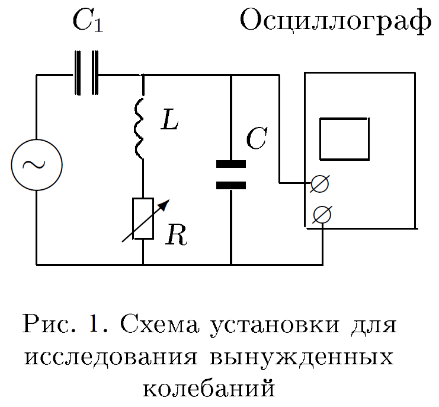
\includegraphics[width=1.99792in,height=1.85in]{./media/image1.png}
Для экспериментального исследования резонансной кривой напряжения в
параллельном колебательном контуре используется схема, изображенная на
рис.~\figref{forced oscillations scheme}. Синусоидальный сигнал с генератора подаётся на параллельный
колебательный контур через небольшую разделительную ёмкость $C_1$.
Напряжение с конденсатора контура $C$ поступает на вертикальный вход
электронного осциллографа (ЭО). Для снятия резонансной кривой
необходимо, чтобы импедансы возбуждающей и измеряющей цепей
(сопротивления переменному току) намного превосходили импеданс самого
контура вблизи резонанса $Z_{\text{рез}} \sim L/(RC) = Q/(\Omega C)$. Разделительная ёмкость
$C_1$ выбирается настолько малой, что в рабочем диапазоне частот её
импеданс $Z_{C_1} = 1/(\Omega C_1)$ много больше импеданса контура, поэтому в цепи
генератора течёт ток практически с постоянной амплитудой, а
колебательный контур выполняет роль нагрузочного сопротивления, которое,
в свою очередь, зависит от частоты. Поскольку в резонансе сопротивление
$Z_\text{рез}$ параллельного контура максимально, то и напряжение на ёмкости $C$
(неизменный ток, умноженный на максимальное сопротивление) тоже
максимально. Входное сопротивление осциллографа (измеряющей цепи)
достаточно велико: $R_{\text{ЭО}} \approx 1$~МОм, поэтому его влиянием можно пренебречь.

Таким образом, при выполнении условий

\begin{equation}
	\eqmark{2.4.1}
Z_{C_1} = \frac{1}{\Omega C_1} \gg \left| Z \right|_{rez} = \frac{Q}{\Omega C}, \qquad R_\text{ЕО} \gg \frac{Q}{\Omega C}
\end{equation}
и при условии, что действительная часть импеданса катушки много меньше
её мнимой части, резонансная кривая в нашем контуре будет выглядеть так
же, как и в последовательном: максимум амплитуды при резонансе. Ширина
резонансной кривой определяет важную характеристику контура~---~\important{добротность}.

\labsection{Б. Процессы установления и затухания колебаний в контуре.}

Добротность контура может быть определена и другими способами, например,
по скорости нарастания амплитуды вынужденных колебаний при резонансе или
по скорости затухания свободных колебаний.

\begin{wrapfigure}[13]{r}{0.45\linewidth}
	\pic{0.45\textwidth}{Chapter_2/2_5_3}
	\caption{Нарастание и затухание вынужденных колебаний}
	\figmark{forced oscillations damping}
\end{wrapfigure}
%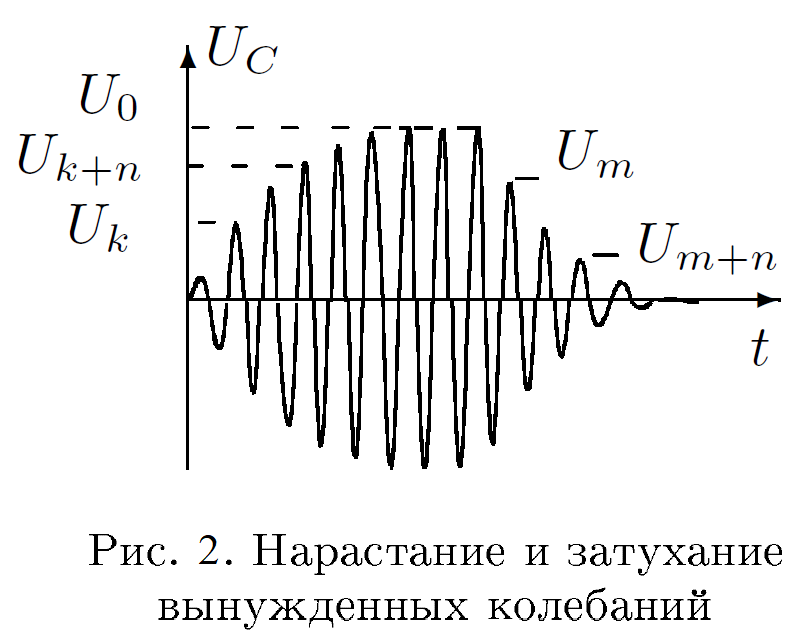
\includegraphics[width=2.72431in,height=2.17778in]{./media/image2.PNG}
Нарастание
и затухание колебаний (рис.~\figref{forced oscillations damping}) можно наблюдать на экране осциллографа,
если на контур подаются цуги~---~отрезки синусоиды, разделённые
интервалами, в течение которых сигнал отсутствует. Чем выше добротность,
тем медленнее нарастают и медленнее затухают колебания в контуре.
Количественные оценки можно сделать, если определить логарифмический
декремент затухания по скорости нарастания или затухания колебаний. В
условиях резонанса огибающая затухающих колебаний~---~это перевёрнутая
огибающая нарастающего участка, поэтому при расчёте логарифмического
декремента по затуханию нет необходимости использовать амплитуду
установившихся колебаний $U_0$, которая в контуре с высокой добротностью
может не успеть установиться за время продолжительности цуга.

\experiment Схема установки для исследования
вынужденных колебаний приведена на рис.~\figref{forced oscillations exp scheme}. Колебательный контур состоит
из конденсатора с ёмкостью $C$, катушки с индуктивностью $L$ и магазина
сопротивлений $R$.

\begin{figure}[h]
	\pic{0.45\textwidth}{Chapter_2/2_5_4}
	\caption{Схема экспериментальной установки для исследования вынужденных
колебаний}
	\figmark{forced oscillations exp scheme}
\end{figure}
%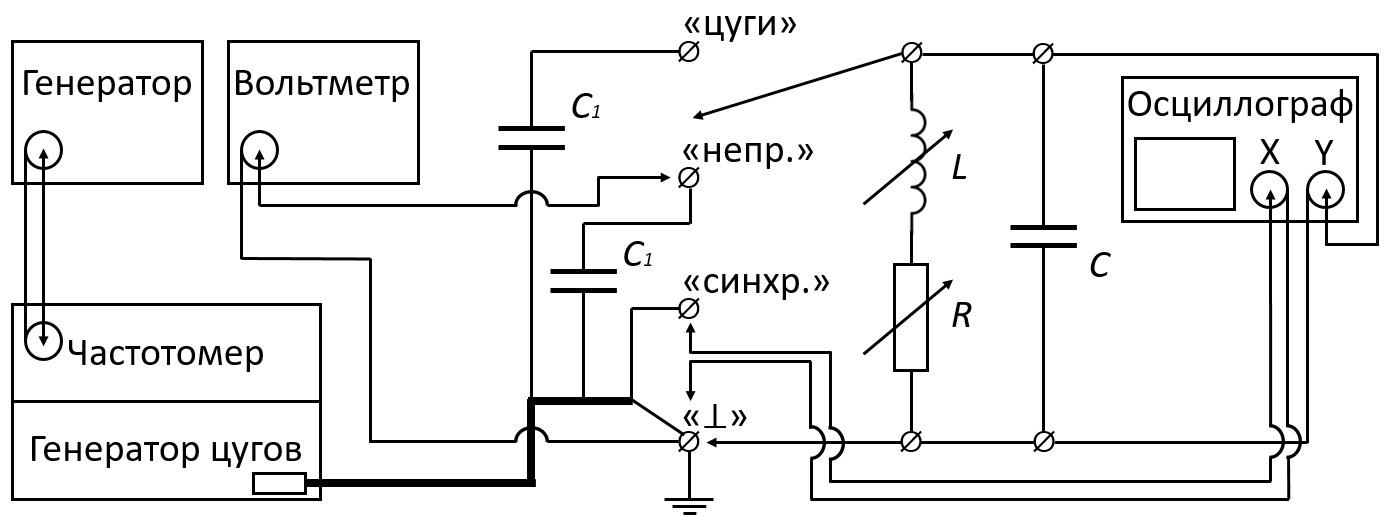
\includegraphics[width=6.49653in,height=2.48056in]{./media/image3.png}
\todo[author=Tiffani]{Рис. 19 немного не соответсвует рис. в ворд-файле}
Синусоидальное напряжение от звукового генератора проходит через
частотомер, позволяющий измерять рабочую частоту с высокой точностью, и
генератор цугов~---~электронное реле, ``разрезающее'' синусоиду на
периодически повторяющиеся цуги~---~отрезки синусоиды.

Затем сигнал через небольшую ёмкость $C_1$ поступает на клеммы,
смонтированные на отдельной панели. При подключении контура к клеммам
«$\perp$» и «непр.» на контур подаётся непрерывный сигнал~---~синусоида; если
контур подключён к клеммам «$\perp$» и «цуги»~---~на контур поступают отрезки
синусоиды.

Для наблюдения за процессом колебаний напряжение с ёмкости подаётся на
вход осциллографа. Чтобы картина на экране была устойчивой, частота
развёртки осциллографа принудительно синхронизуется с частотой
повторения цугов. Для этого на генератор развёртки ЭО подаются следующие
с частотой повторения цугов управляющие импульсы, которые вырабатываются
в блоке электронного реле (клемма «синхр», смонтированная на панельке).
Для измерений напряжения на ёмкости используется электронный вольтметр.

\begin{lab:task}

В работе предлагается при двух значениях сопротивления магазина
исследовать резонансные кривые и определить по ним добротность контура;
затем определить добротность, определив логарифмический декремент
затухания при нарастании и при затухании колебаний.

	\begin{enumerate}
	\tasksection{I. Подготовка приборов к работе}

	\item Соберите схему согласно рис.~\figref{forced oscillations exp scheme} и подключите контур к клеммам «$\perp$» и
«непр.». Включите приборы в сеть. Руководствуясь техническим описанием,
расположенным у установки, настройте генератор, осциллограф, проверьте
работоспособность источника питания, а также выставите необходимые
значения на магазинах сопротивлений и индуктивностей.

\tasksection{II.Исследование резонансных кривых}

	\item Рассчитайте собственную частоту контура
($\nu_{0} = 1/2\pi\sqrt{LC}$).

	\item Изменяя частоту генератора вблизи резонансной и наблюдая за
синусоидой на экране осциллографа, убедитесь, что в резонансе амплитуда
колебаний максимальна. Подберите частоту развёртки осциллографа и
амплитуду синхронизации, при которых картина неподвижна.

	\item Меняя частоту генератора в обе стороны от резонансной, снимите
зависимость показаний вольтметра $U$ от показаний частотомера
$\nu$. Расчёт добротности ведётся на уровне $0,7$ от резонансной
амплитуды, поэтому стоит аккуратнее провести измерения в районе этого
уровня, а также продолжать измерения по крайней мере до тех пор, пока
амплитуда сигнала упадёт до величины $0,3 - 0,4$ от резонансной.

	\item Установите на магазине сопротивлений другое значение, заданное
преподавателем, и повторите измерения п.4. Закончив измерения, отключите
вольтметр от сети.

\tasksection{III.Процессы установления и затухания колебаний}

	\item Подключите контур к клеммам «цуги» и «$\perp$». Выведите до нуля
сопротивление магазина.

	\item Установите на генераторе резонансную частоту. Подберите частоту
развёртки осциллографа, при которой на экране умещается один цуг
колебаний. Убедитесь, что огибающая затухающих колебаний это
перевёрнутая огибающая нарастающего участка. Если они заметно отличаются
(реле может внести искажения), то следует уменьшить амплитуду сигнала с
генератора.

	\item Для расчёта добротности по скорости нарастания амплитуды измерьте
амплитуды двух колебаний $U_k$ и $U_{k+n}$, разделённых целым числом периодов $n$,
и амплитуду установившихся колебаний $U_0$ (см. рис.~\figref{forced oscillations damping}).

Перед началом измерений заземлите канал $Y$, чтобы уточнить положение оси
$X$~---~начала отсчёта амплитуды. Можно увеличить амплитуду, сместив
горизонтальную ось симметрии цуга в нижнюю часть экрана. Расчёт будет
тем точнее, чем больше отличаются друг от друга все три амплитуды.

Проведите измерения для 3 -- 4-х пар амплитуд.

	\item Для определения добротности по скорости затухания измерьте две
амплитуды, разделённые целым числом периодов (для 3 -- 4-х пар амплитуд).

	\item Повторите измерения п.8 и п.9 для другого значения сопротивления,
заданного преподавателем.

	\item Сместите частоту генератора от резонансного значения и получите на
экране картину биений. Зарисуйте и объясните эту картину.

	\item Отключите приборы от сети и разберите схему.

	\item Измерьте активное сопротивление $R_L$ и индуктивность $L$ магазина
индуктивностей с помощью измерителя $LCR$ на частотах $50$~Гц, $500$~Гц и $1500$~Гц.

\tasksection{IV.Обработка результатов}

	\item Постройте на одном графике резонансные кривые в координатах $U/U0 = f(
\nu/\nu_0)$, где $U_0$~---~напряжение при резонансной частоте $\nu_0$.

Определите добротность по формуле $Q = \omega_0/(2\Delta\Omega)$. Сравните теоретическое и
экспериментальное значения резонансной частоты.

	\item Рассчитайте добротность контура по скорости нарастания и затухания
колебаний.

	\item Рассчитайте теоретическое значение добротности через параметры
контура $L$, $C$ и $R$.

	\item Сведите результаты определения $Q$ в таблицу:

	\begin{center}
\begin{tabular}{|c|c|c|c|c|c|}
\hline
& & \multicolumn{4}{c|}{$Q$}\\
\cline{3-6}
$R$, Ом & $R_{\text{конт}}$ & & & &$f(LCR)$\\
\hline
$0$ & & & & & \\
$100$ & & & & &\\
\hline
\end{tabular}
\end{center}
\todo[author=Tiffani]{Как вставить данные символы в таблицу(см. рисунок)?}

\begin{figure}[h!]
	\centering
	%\pic{0.6\linewidth}{Chapter_2/image4}
	\caption{Таблица}
\end{figure}

%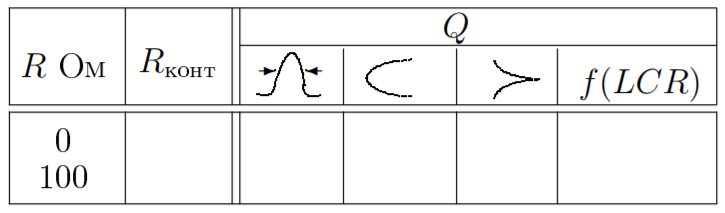
\includegraphics[width=3.37592in,height=0.99167in]{./media/image4.png}
	\item Оцените погрешности и сравните результаты расчётов.
	\end{enumerate}
\end{lab:task}

\todo[author=Tiffani]{Нет вопросов после лабораторной}

\begin{lab:literature}
	\item \emph{Сивухин~Д.В.} Общий курс физики. -- Т.III. Электричество. -- ~М.:~Физматлит,~2004. \S\S~122 -- 124.

	\item \emph{Калашников~С.Г.} Электричество. --~М.:~Физматлит, 2008. \S\S~207 -- 210.
\end{lab:literature}

\lab{Свободные колебания в электрическом контуре}

\begin{lab:aim}
исследование свободных колебаний в колебательном контуре.
\end{lab:aim}

\begin{lab:equipment}
генератор импульсов, электронное реле, магазин сопротивлений, магазин ёмкостей,
катушка индуктивности, электронный осциллограф, универсальный мост.
\end{lab:equipment}

Перед выполнением работы необходимо ознакомиться с п.~\ref{sec:free}
введения к данному разделу.

В работе исследуется колебательный контур, состоящий 
из индуктивности $L$, ёмкости $C$ и резистора $R$ (см. рис.~\chapterfigref{fig1}). 
Конденсатор контура заряжается короткими
одиночными импульсами, после каждого из которых в контуре возникают свободные
затухающие колебания. Подав напряжение с конденсатора на осциллограф, можно по
изображению на экране осциллографа определить период свободных колебаний в
контуре, исследовать их затухание и определить основные параметры колебательного
контура.

%\begin{figure}[h]
\begin{wrapfigure}[15]{r}{0.45\linewidth}
	\pic{0.4\textwidth}{Chapter_2/2_4_1}
	\caption{Схема установки для наблюдения затухающих колебаний на фазовой
плоскости}
	\figmark{fig1}
\end{wrapfigure}
%\end{figure}

Картину колебаний можно представить не только в координатах ($U$,~$t$)
(рис.~\chapterfigref{fig2}а), 
но и в координатах $(U,\,I)$ на так называемой \emph{фазовой плоскости} 
(рис.~\figref{fig2}б). В этих координатах кривая
незатухающих колебаний (при $\gamma~=~0$) имеет вид эллипса, а картина реальных
затухающих колебаний представляет собой сворачивающуюся спираль.

Принципиальная схема подключения осциллографа для изучения колебаний на фазовой
плоскости изображена на рис.~\figref{fig1}. На вертикальный вход
осциллографа подаётся напряжение $U_C$ с конденсатора, а на
горизонтальный~--- напряжение с резистора $U_R$ 
($U_R \propto I = dq/dt \propto dU_C/dt$).

\experiment 
На рис.~\figref{fig2} приведена схема для исследования
свободных колебаний в контуре, содержащем постоянную индуктивность $L$ и
переменные ёмкость $C$ и сопротивление $R$. Картина колебаний наблюдается на
экране осциллографа.


Для периодического возбуждения колебаний в контуре используется генератор
импульсов. С~выхода генератора сигналы поступают на колебательный контур через
электронное реле, которое содержит диодный тиристор~$D$ и ограничительный
резистор~$R_1$. Тиристор без управляющего электрода представляет собой
полупроводниковый ключ, открывающийся при напряжении на нём выше порогового, и
закрывающийся при любом напряжении другого знака. Благодаря этому генератор
отключается от колебательного контура после каждого импульса, и внутреннее
сопротивление генератора не влияет на процессы в колебательном контуре.

Каждый импульс заряжает конденсатор~$C$, после чего в контуре возникают
свободные затухающие колебания. Входное сопротивление осциллографа велико,
поэтому его влиянием на контур можно пренебречь.

\begin{figure}[h!]
    \centering
	\pic{0.95\textwidth}{Chapter_2/2_4_2}
	\caption{Схема установки для исследования свободных колебаний}
	\figmark{fig2}
\end{figure}

\begin{lab:task}

\taskpreamble{В работе предлагается исследовать зависимость периода свободных
колебаний контура от ёмкости, зависимость логарифмического декремента затухания от
сопротивления, определить критическое сопротивление и добротность контура.}

\tasksection{I. Подготовка приборов к работе}


	\item Соберите схему согласно рис.~\figref{fig2}. Подключите
выход генератора через реле к магазину ёмкостей таким образом, чтобы можно было
менять ёмкость в интервале 0--1~мкФ.

	\item Установите на генераторе длительность импульсов $5$~мкс, а частоту
повторения импульсов $\nu_0 = 100$~Гц ($T = 0,01$~c).

	\item Настройте осциллограф, руководствуясь техническим описанием,
расположенным на установке.

\tasksection{II. Измерение периодов свободных колебаний}

	\item Установите на магазине сопротивлений величину $R = 0$; на магазине
ёмкостей~---~величину $C = 0,02$~мкФ.

	\item Подберите частоту развёртки осциллографа, при которой расстояние между
импульсами, поступающими с генератора, занимает почти весь экран.

	\item Измерьте расстояние, которое занимают несколько полных периодов $n$.
Проверьте, совпадают ли период повторения импульсов на генераторе с периодом
повторения импульсов, измеренным при помощи горизонтальной шкалы осциллографа.
При несовпадении периодов прокалибруйте горизонтальную шкалу осциллографа по
известному периоду повторения импульсов.

	\item Измерьте на экране осциллографа расстояние $x$, которое занимают
несколько полных периодов $n$. Рассчитайте период свободных колебаний контура.
Малые расстояния $x$ можно увеличить кнопкой растяжки развёртки.

	\item Изменяя ёмкость от $0,02$~мкФ до $0,9$~мкФ, проведите измерения
периодов свободных колебаний (8--10 значений).

\tasksection{III. Измерение критического сопротивления и декремента затухания}


	\item Для данной в работе индуктивности рассчитайте ёмкость~$C$, при которой
собственная частота колебаний контура $\nu_0 = 1/(2\pi\sqrt{LC})$ составляет
$5$~кГц. Для выбранных значений~$L$ и~$C$ рассчитайте критическое сопротивление
контура $R_\text{кр} = 2\sqrt{L/C}$.

	\item Установите на магазине ёмкость, близкую к рассчитанной. Увеличивая
сопротивление $R$ от нуля до  $R_\text{кр}$, наблюдайте картину затухающих
колебаний на экране осциллографа. Зафиксируйте сопротивление магазина, при
котором колебательный режим переходит в апериодический. Сравните значения
найденного экспериментально и рассчитанного значения  $R_\text{кр}$.

	\item Установите сопротивление $R \simeq 0,1 R_\text{кр}$. Получите
на экране картину затухающих колебаний. Для расчёта логарифмического декремента
затухания $\Theta$ по формуле \chaptereqref{2.27} измерьте амплитуды,
разделенные целым числом периодо $n$. Расчёт будет тем точнее, чем больше
отличаются друг от друга измеряемые амплитуды, а минимальная не должна быть
меньше 5--6~мм.

	\item Повторите измерения для 6--8 значений $R$ в интервале $(0,1-0,3)R_\text{кр}$.

\tasksection{IV. Свободные колебания на фазовой плоскости}


	\item Для наблюдения затухающих колебаний на фазовой плоскости подайте на
вход «Х» осциллографа напряжение с магазина сопротивлений. Переведите
осциллограф в режим измерения «X--Y». Изменяя чувствительность каналов,
подберите масштаб спирали. При том же значении ёмкости что и в п.~10, наблюдайте
за изменением спирали при увеличении сопротивления от $0,1R_\text{кр}$  до
$0,3R_\text{кр}$. Для определения $\Theta$~измерьте радиусы витков спирали,
разделённые целым числом периодов $n$, для одного-двух значений $R$ на каждом
краю рабочего диапазона.

	\item Отсоедините катушку от цепи. С помощью измерителя $LCR$ измерьте
омическое сопротивление $R_L$ и индуктивность $L$ катушки на частотах $50$~Гц,
$1$~кГц и $5$~кГц. Подумайте, почему результат измерения омического
сопротивления катушки зависит от частоты.

\tasksection{V. Обработка результатов}

	\item Рассчитайте экспериментальные значения периодов по результатам
измерений и теоретические по формуле \chaptereqref{2.7}. 
Постройте график $T_\text{эксп} = f(T_\text{теор})$.

	\item Рассчитайте значения логарифмического декремента 
    затухания $\Theta$ (п.~12) и сопротивления контура $R_{\Sigma}$ 
    (сопротивление контура состоит из сопротивления магазина $R$ и 
    омического сопротивления катушки $R_L$).

Постройте график в координатах $1/\Theta^2 =f[1/R^2_{\Sigma}]$. 
Убедитесь в линейности зависимости и по наклону прямой 
определите критическое сопротивление~$R_\text{кр}$ (см.
формулы \chaptereqref{2.30}). 
%С помощью равенств
%\chaptereqref{2.6}, \chaptereqref{2.23}, \chaptereqref{2.27}, и
%\chaptereqref{2.38} 
%и приняв обозначения $1/\Theta^2~=~Y$, $1/
%R^2_\text{конт}~=~X$, покажите, что $R_\text{кр} = 2\pi\sqrt{\Delta Y / \Delta
%X}$.

	\item Рассчитайте теоретическое значение $R_\text{кр} = 2\pi\sqrt{L / C}$
и сравните его с измеренным.

	\item Рассчитайте добротность контура $Q$ для максимального и минимального
значений~$\Theta$ по картине затухающих колебаний и сравните с расчётом $Q$
через параметры контура~$R$, $L$ и~$C$  \chaptereqref{2.35}.

	\item Рассчитайте добротность $Q$ по спирали.

	\item Сведите результаты эксперимента в таблицу:

\begin{center}\small
\begin{tabular}{|c|c|c|c|c|c|c|c|}
\hline
& \multicolumn{3}{c|}{$R_{\text{кр}}$} &  & \multicolumn{3}{c|}{$Q$} \\
\cline{2-4}
\cline{6-8}
$L_{\text{кат}}$ & $\text{Теор.}$ & $\text{Подбор}$ & $\text{Граф.}$ & $R$ &
$\text{Теор.}$ & $f(\Theta)$ & $\text{Спираль}$  \\
\hline
& & & & $\text{max}$ & & &  \\
& & & & $\text{min}$ & & &  \\
\hline
\end{tabular}
\end{center}

	\item Оцените погрешности и сравните результаты. Какой из методов
определения $R_\text{кр}$ и $Q$ точнее? Почему?

\end{lab:task}


\begin{lab:questions}
	\item Что такое собственная частота, добротность, логарифмический декремент
затухания колебательного контура?
    \item Как отличаются периоды свободных колебаний с затуханием и без затухания?
	\item Что называют фазовой плоскостью колебаний?
	\item  Как определить логарифмический декремент затухания по картине
колебаний в фазовой плоскости?
	\item  Возможно ли вызвать резонанс в колебательном контуре при помощи
периодических импульсов?
\end{lab:questions}


\begin{lab:literature}
	\item \SivuhinIII~--- \S\S~122~--~124.
	\item \Kalashnikov~--- \S\S~207~--~210.
\end{lab:literature}

\lab{Исследование гальванометра}
\label{lab:galvanometr}

\aim{изучение работы высокочувствительного зеркального
гальванометра магнитоэлектрической системы в режимах измерения
постоянного тока и электрического заряда.}

\equip{зеркальный гальванометр с осветителем и
шкалой, источник постоянного напряжения, делитель напряжения, магазин
сопротивлений, эталонный конденсатор, вольтметр, переключатель, ключи,
линейка.}

Баллистическим гальванометром называют электроизмерительный прибор
магнитоэлектрической системы, отличающийся высокой чувствительностью к
току и сравнительно большим периодом колебаний подвижной системы
(рамки).

Главной частью баллистического гальванометра является подвешенная на
вертикальной нити рамка, помещённая в поле постоянного магнита. Вырез
цилиндрической формы в полюсах магнита и ферромагнитный цилиндр на оси
системы делают поле в зазоре радиальным (рис.~\figref{current loop}). 
Скреплённое с рамкой
зеркальце служит для измерения угла поворота рамки. К рамке прикреплён
полый цилиндр, который сильно увеличивает момент инерции и,
следовательно, период колебаний подвижной системы, не очень её утяжеляя.
Магнит и подвижная система заключены в защитный кожух. В баллистических
гальванометрах применяют сильные постоянные магниты и рамки с большим
количеством витков, подвешенные на тонких нитях с малой упругостью.

Баллистический гальванометр позволяет измерять как постоянный ток
(стационарный режим), так и заряд, протекший через рамку за некоторое
время (баллистический режим). В баллистическом режиме гальванометр может
работать, если время протекания заряда много меньше периода собственных
колебаний подвижной рамки. Поэтому период колебаний рамки делают большим
(5~--~15~с). Это время учитывает реакцию экспериментатора, которому надо
успеть сделать отсчёт максимального отклонения рамки.

\labsection{Уравнение движения подвижной системы}
На помещённую в магнитное
поле обтекамую током рамку гальванометра действуют следующие моменты
сил: момент закрученной нити, момент магнитных сил и тормозящий момент,
зависящий от сил сопротивления воздуха и от вихревых токов, вызывающих
электромагнитное торможение. Рассмотрим каждый из этих моментов в
отдельности.

Механический момент $M_1$ упругих сил нити
пропорционален углу поворота рамки:

\begin{equation}
	\eqmark{2.6.1}
	M_1 = -D\varphi,
\end{equation}
где $D$~---~модуль кручения нити, а $\varphi$~---~угол поворота рамки 
от положения равновесия.

\begin{figure}[h]
	\pic{0.8\textwidth}{Chapter_2/2_6_1}
	\caption{Рамка с током в магнитном поле}
	\figmark{current loop}
\end{figure}

Если рамка с числом витков $N$, обтекаемая током $I$, помещена
в магнитное поле с индукцией $B$, то на боковые стороны рамки
(перпендикулярные чертежу на рис.~
\figref{current loop}) действуют силы, равные $lNBI$,
где $l$~---~длина боковой стороны. Обозначив через $r$ расстояние от
боковой стороны до оси вращения, найдём момент пары сил
\begin{equation}
	\eqmark{2.6.2}
	M_2 = 2rlBNI = BSNI,
\end{equation}
где $S$~---~площадь одного витка рамки.

Тормозящий момент складывается из моментов сил электромагнитного
торможения и сил трения о воздух. В рамке, движущейся в магнитном поле с
угловой скоростью $\dot{\varphi}$, наводится ЭДС индукции
\begin{equation}
	\eqmark{2.6.3}
	E_{\text{инд}} = -\frac{d\Phi}{dt} = -BSN\dot{\varphi},
\end{equation}
где $\Phi$~---~магнитный поток, пронизывающий рамку. Пренебрегая самоиндукцией
рамки, можно считать, что эта ЭДС вызывает ток индукции 
$I_{\text{инд}} = -E_{\text{инд}}/R_{\scriptscriptstyle \sum}$, 
где $R_{\scriptscriptstyle \sum}$~---~полное
сопротивление цепи, состоящее из сопротивления рамки и сопротивления
внешнего участка цепи $R$:
\begin{equation}
	\eqmark{2.6.4}
	R_{\scriptscriptstyle \sum} = R_0 + R.
\end{equation}
Связанный с ЭДС индукции тормозящий момент
\begin{equation}
	\eqmark{2.6.5}
	M_3 = BSNI_{\text{инд}} = - (BSN)^2 R^{-1}_{\scriptscriptstyle \sum}\dot{\varphi}.
\end{equation}
Обычно этот момент значительно превосходит момент сил трения рамки о
воздух, которым мы и пренебрежём для простоты расчёта.

Уравнение движения рамки $J\ddot{\varphi} = M_{\scriptscriptstyle \sum}$, 
где $J$~---~момент инерции подвижной системы, а $M_{\scriptscriptstyle \sum}$~---~
сумма моментов, даваемых формулами \eqref{2.6.1}, \eqref{2.6.2}, \eqref{2.6.4}, 
представляется в виде:
\begin{equation}
	\eqmark{2.6.6}
	\ddot{\varphi} + 2\gamma \dot{\varphi} + \omega^2_{0}\varphi = KI.
\end{equation}
Здесь ток $I = E/R_{\scriptscriptstyle \sum}$ определяется величиной 
ЭДС $E$ внешнего источника, к которому подключён гальванометр, и полным 
сопротивлением цепи $R_{\scriptscriptstyle \sum}$, а параметры $\gamma$, 
$\omega_0$ колебательной системы и коэффициент $K$ связаны с параметрами 
гальванометра формулами:
\begin{equation}
	\eqmark{2.6.7}
	K = \frac{BNS}{J}, \qquad 2\gamma = \frac{(BSN)^2}{JR_{\scriptscriptstyle \sum}}, 
    \qquad \omega^2_0 = \frac{D}{J}.
\end{equation}
Отметим, что заменой переменой $\varphi$ на 
$\tilde{\varphi} = \varphi - KI/\omega^2_0$ уравнение \eqref{2.6.6} приводится 
к однородному уравнению вида \chaptereqref{2.8}, описывающему свободные 
затухающие колебания в $RCL$-контуре, рассмотренные в теоретической части 
Раздела II.

\labsection{Режим измерения постоянного тока}
Если через рамку пропускать постоянный ток (достаточно долго, чтобы затухли 
колебания подвижной системы), то в уравнении \eqref{2.6.6} можно положить 
$\dot{\varphi} = 0$, $\ddot{\varphi} = 0$, так что угол поворота рамки 
определится формулами
\begin{equation}
	\eqmark{2.6.8}
	\varphi = \frac{K}{\omega^2_0}I = \frac{BSN}{D}I = S_I I = \frac{I}{C_I},
\end{equation}
где величина $S_I = \varphi/I = BSN/D$ называется 
\important{чувствительностью гальванометра} к току, а
обратная её величина $C_I = 1/S_I = I/\varphi = D/BSN$~--- 
\important{постоянной гальванометра}.

\labsection{Свободные колебания рамки} Исследуем свободное движение рамки,
т.~е. движение в отсутствие внешних источников тока, когда $I = 0$. В этом
случае уравнение \eqref{2.6.6} для угла поворота рамки $\varphi$ примет вид
\begin{equation}
	\eqmark{2.6.9}
	\ddot{\varphi} + 2\gamma \dot{\varphi} + \omega^2_{0}\varphi = 0,
\end{equation}
аналогичный уравнению \chaptereqref{2.8}, так что мы можем воспользоваться решениями,
полученными в соответствующем разделе сборника, учтя, однако, начальные
условия рассматриваемой здесь задачи. Примем, что эти условия таковы:
\begin{equation}
	\eqmark{2.6.10}
	 \varphi(0) = 0, \qquad \dot{\varphi} = \dot{\varphi_0},
\end{equation}
т.~е. рамке сообщили начальную угловую скорость без заметного
начального смещения. Рассмотрим возможные случаи движения рамки.
\begin{enumerate}
	\item $\gamma < \omega_0$ (колебательный режим).

Решение уравнения \eqref{2.6.9}, удовлетворяющее начальным условиям \eqref{2.6.10}, 
имеет в этом случае вид
\begin{equation}
	\eqmark{2.6.11}
	 \varphi(t) = \frac{\dot{\varphi_0}}{\omega_1} e^{- \gamma t} \sin{\omega_1 t}, 
     \qquad \omega_1 = \sqrt{\omega_0^2 - \gamma^2}.
\end{equation}
Движение рамки носит колебательный характер и затухает со временем.
Период колебаний при этом равен
\begin{equation}
	\eqmark{2.6.12}
	 T_1 = \frac{2\pi}{\omega_1} = 
     \frac{2\pi}{\sqrt{D/J - (BSN)^4/(2JR_{\scriptscriptstyle \sum})^2}},
\end{equation}
а коэффициент затухания $\gamma$ определяется формулами \eqref{2.6.7} и \eqref{2.6.4}. 
При малом затухании, когда $\gamma \ll \omega_0$, $\omega_1 \approx \omega_0$, 
движение рамки близко к синусоидальному:
\begin{equation}
	\eqmark{2.6.13}
	 \varphi(t) = \frac{\dot{\varphi_0}}{\omega_0} \sin{\omega_0 t}.
\end{equation}

	\item $\gamma = \omega_0$(критический режим). Этот режим реализуется при 
    сопротивлении внешнего участка цепи $R$ из формулы \eqref{2.6.4}, равном 
    \important{критическому сопротивлению}
\begin{equation}
	\eqmark{2.6.14}
	 R_{\text{кр}} = R_{\scriptscriptstyle \sum\text{кр}} - R_0 = \frac{(BSN)^2}{2\sqrt{DJ - R_0}}.
\end{equation}
Решение уравнения \eqref{2.6.9} при начальных условиях \eqref{2.6.10} в этом 
случае имеет вид
\begin{equation}
	\eqmark{2.6.15}
	 \varphi(t) = \dot{\varphi_0} t e^{- \gamma t}.
\end{equation}
Движение не имеет колебательного характера: отклонённая после начального
толчка подвижная система почти экспоненциально возвращается к нулю.

	\item $\gamma \gg \omega_0$(затухание велико~---~случай переуспокоенного 
    гальванометра). Решение уравнения \eqref{2.6.9} при этом имеет вид

\begin{equation}
	\eqmark{2.6.16}
	 \varphi(t) = \frac{\dot{\varphi_0}}{\alpha} e^{- \gamma t} \sh{\alpha t}, 
     \qquad \alpha = \sqrt{\gamma^2 - \omega_0^2}.
\end{equation}
Движение остаётся апериодическим, однако подвижная система приближается
к равновесию медленнее, чем в критическом режиме.
\end{enumerate}

\labsection{Режим измерения заряда}
Как уже было отмечено, период свободных
колебаний баллистического гальванометра благодаря искусственному
увеличению момента инерции рамки оказывается очень большим (порядка
десяти секунд). Если пропустить через рамку короткий импульс тока, то
можно считать, что весь ток успевает пройти при неотклонённом положении
рамки. Рамка, однако, при этом получает толчок, в результате которого
возникает движение, описываемое уравнением свободных колебаний \eqref{2.6.9} при
начальных условиях \eqref{2.6.10}.

Для вычисления угловой скорости $\dot{\varphi_0}$, полученной в результате толчка,
проинтегрируем уравнение \eqref{2.6.6} по времени от $0$ до $\tau$~---~момента 
окончания токового импульса. В результате приходим к соотношению
\begin{equation}
	\eqmark{2.6.17}
	 \dot\varphi(\tau) + 2\gamma\varphi(\tau) + 
     \omega_0^2 \int\limits_0^\tau \varphi(t) dt = 
     Kq,
\end{equation}
где $q = \int\limits_0^\tau I dt$~---~полный электрический заряд, прошедший 
через рамку гальванометра за
время импульса. При малом начальном отклонении рамки и малой
длительности импульса можно пренебречь вторым и третьим слагаемыми в
\eqref{2.6.16}, связанными соответственно с током индукции и упругостью нити.
Уравнение \eqref{2.6.16} в этом случае принимает вид:
\begin{equation}
	\eqmark{2.6.18}
	 \dot\varphi(\tau) = Kq.
\end{equation}
Таким образом, при пропускании короткого импульса тока через
баллистический гальванометр начальная угловая скорость движения рамки
пропорциональна полному электрическому заряду, прошедшему через рамку за
всё время импульса. Подставляя выражения \eqref{2.6.11}, \eqref{2.6.14} или \eqref{2.6.15}, легко
увидеть, что наибольший угол, на который отклоняется рамка, также
пропорционален $q$.

Величина $C_Q = q/\varphi_{max}$ называется \important{баллистической постоянной} 
гальванометра. Баллистическая постоянная наряду с динамической является важнейшей
характеристикой гальванометра, но в отличие от динамической она
существенно зависит от режима работы гальванометра (от сопротивления
цепи). Величина $S_Q = 1/C_Q$ называется \important{чувствительностью гальванометра к
заряду}.

Выбирая оптимальный режим работы, приходится одновременно исходить из
двух противоречивых требований: желания получить максимальную
чувствительность гальванометра к заряду и стремления по возможности
сократить время, затрачиваемое на измерения.

Расчёт показывает, что максимальный отброс достигается при полном
отсутствии затухания (тормозящий индукционный ток отсутствует при обрыве
в цепи):
\begin{equation}
	\eqmark{2.6.19}
	 \varphi_{max} = \frac{\dot\varphi(\tau)}{\omega_0} = \frac{Kq}{\omega_0}.
\end{equation}
В этом случае, однако, возникшие в результате отброса колебания рамки не
будут успокаиваться, и прибор не скоро сможет быть использован для
повторных измерений. Поэтому обычно заботятся о том, чтобы затухание
гальванометра не было слишком малым. Кроме того, отметим, что затухание
приводит к тому, что зайчик начинает вести себя более спокойно и слабее
реагирует на посторонние электрические и механические импульсы.

Обычно удобнее всего работать в режиме, близком к критическому. При этом
обеспечивается быстрое затухание колебаний, и чувствительность прибора
достаточно велика.

Как следует из уравнения \eqref{2.6.14}, в случае критического затухания
\begin{equation}
	\eqmark{2.6.20}
	 \varphi_{max \text{кр}} = \frac{\dot\varphi(\tau)}{\omega_0} = 
     \frac{Kq}{\omega_0 e}.
\end{equation}
Таким образом, в критическом режиме максимальное отклонение зайчика в $e$
раз меньше, чем в режиме свободных колебаний. Отсюда, в частности,
следуют соотношения
\begin{equation}
	\eqmark{2.6.21}
	 \frac{C_{Q \text{кр}}}{C_{Q \text{св}}} = 
     \frac{S_{Q \text{св}}}{S_{Q \text{кр}}} = e
\end{equation}
между баллистическими постоянными и чувствительностями гальванометра,
работающего в режиме свободных колебаний (св) и в критическом (кр)
режиме.

\labsection{A. Определение динамической постоянной гальванометра}

\experiment
Схема для исследования
гальванометра в стационарном режиме представлена на 
рис.~\figref{scheme galvanometer steady}. Постоянное
напряжение $U \simeq 1,5$ В снимается с блока питания и измеряется вольтметром $V$. 
Ключ $K_3$ позволяет менять направление тока через гальванометр Г, делитель
напряжения~---~менять величину тока в широких пределах. Ключ $K_2$ служит для
включения гальванометра, кнопка $K_1$~---~для его успокоения. Магазин
сопротивлений $R$ позволяет менять режим работы гальванометра от
колебательного до апериодического.

\begin{figure}[h]
	\pic{0.9\textwidth}{Chapter_2/2_6_2}
	\caption{Схема установки для работы гальванометра в стационарном режиме}
	\figmark{scheme galvanometer steady}
\end{figure}

При $R_1 \ll R, R_0, R_2$ сила тока, протекающего через гальванометр, может 
быть вычислена по очевидной формуле:
\begin{equation}
	\eqmark{2.6.22}
	 I = \frac{R_1}{R_2} \frac{U_0}{R + R_0},
\end{equation}
где $U_0$~---~показания вольтметра, $I = R_1/R_2$~---~положение делителя, 
$R$~---~сопротивление магазина, $R_0$~---~внутреннее сопротивление гальванометра.

Угол отклонения рамки от положения равновесия измеряется с помощью
осветителя, зеркальца, укреплённого на рамке, и шкалы, на которую
отбрасывается луч света от зеркальца. Координата $x$ светового пятна на
шкале связана с углом $\varphi$ отклонения рамки формулой
\begin{equation}
	\eqmark{2.6.23}
	x = a \arctg{(2\varphi)},
\end{equation}
где $a$~---~расстояние от шкалы до зеркальца. При малых углах можно считать,
что $\varphi = x/2a$. Динамическую постоянную
\begin{equation}
	\eqmark{2.6.24}
	C_I = \frac{I}{\varphi} = \frac{2aI}{x},
\end{equation}
как правило, выражают в единицах $\frac{\text{А}}{\text{мм}/\text{м}}$ 
(ток $I$ измеряется в амперах, $x$~---~в мм, $a$~---~в
метрах).

\labsection{Б. Определение критического сопротивления гальванометра}

Критическим сопротивлением баллистического гальванометра называется
сопротивление его электрической цепи $R_{\text{кр}}$, при котором после начального
толчка подвижная система почти экспоненциально возвращается к нулю,
подчиняясь уравнению \eqref{2.6.14}. Как отмечалось в теоретическом введении к
Разделу II, на практике критический режим, требующий строгого выполнения
условия $\gamma = \omega_0$, не может быть точно реализован и имеет значение как
пограничный между режимом затухающих колебаний ($\gamma < \omega_0$) и режимом
апериодического затухания ($\gamma > \omega_0$).

Измерение критического сопротивления гальванометра можно выполнить с
помощью той же схемы (рис.~\figref{scheme galvanometer steady}).

При больших $R$ свободное движение рамки имеет колебательный
характер. С уменьшением $R$ затухание увеличивается 
(см. \eqref{2.6.4}, \eqref{2.6.7}), и колебательный режим переходит в апериодический.

В качестве характеристики процесса затухания колебаний рамки
гальванометра воспользуемся представленым формулой \chaptereqref{2.25}
логарифмическим декрементом затухания
\begin{equation}
	\eqmark{2.6.25}
	\Theta = \gamma T_1 = \ln \frac{x_n}{x_{n+1}},
\end{equation}
где $x_n$ и $x_{n+1}$~---~два последовательные отклонения колеблющейся величины 
в одну сторону. Измеряя зависимость $\Theta(R)$ логарифмического декремента 
затухания от сопротивления внешней цепи $R$, можно найти критическое 
сопротивление $R_{\text{кр}}$ по формуле, которая следует из 
выражений \eqref{2.6.14} и \eqref{2.6.25}:
\begin{equation}
	\eqmark{2.6.26}
	\frac{R_{\text{кр}}}{R_0} = \frac{1 + R/R_0}{\sqrt{1 + [2\pi/\Theta(R)]^2}} - 1.
\end{equation}
Напомним, что сопротивление $R_{\text{кр}}$ связано с параметрами баллистического
гальванометра формулой \eqref{2.6.14}.

\labsection{В. Определение баллистической постоянной и критического
сопротивления гальванометра, работающего в баллистическом режиме}

Для изучения работы гальванометра в режиме измерения заряда, а значит, в
баллистическом режиме, используется схема, представленная на 
рис.~\figref{scheme ballistic constante}.

Система ключей устроена так, что нормально ключ
$K_2$ замкнут, а ключи $K_3$ и
$K_4$ разомкнуты. При нажатии на кнопку
$K_0$ сначала размыкается ключ
$K_2$, затем замыкаетс $K_3$ и
через некоторое время~---~$K_4$. При нормальном
положении кнопки $K_0$ конденсатор $C$
заряжается до напряжения $U_C$ и получает заряд $q$:
\begin{equation}
	\eqmark{2.6.27}
	U_C = \frac{R_1}{R_2}U_0, \qquad q = C U_C = \frac{R_1}{R_2}U_0 C.
\end{equation}

При нажатии на ключ $K_0$ конденсатор отключается от
источника постоянного напряжения (размыкается ключ
$K_2$) и подключается к гальванометру (замыкается
ключ $K_3$).

\begin{figure}[h]
	\pic{0.9\textwidth}{Chapter_2/2_6_3}
	\caption{Схема установки для определения баллистической постоянной}
	\figmark{scheme ballistic constante}
\end{figure}

Ёмкость конденсатора выбрана так, что к моменту замыкания ключа
$K_4$ весь заряд успевает пройти через гальванометр,
и рамка получает начальную скорость $\dot\varphi(\tau)$ (см.~\eqref{2.6.18}). 
При этом можно считать,
что отклонение рамки, происходящее за время, протекающее между
замыканием ключей $K_3$ и $K_4$,
равно нулю. При замыкании ключа $K_4$ гальванометр
шунтируется внешним сопротивлением $R$, и в зависимости от величины
этого сопротивления движение рамки описывается одним из уравнений: \eqref{2.6.11},
\eqref{2.6.13}, \eqref{2.6.15} или \eqref{2.6.16}.

Первый отброс зайчика $l_{max}$ после нажатия на кнопку $K_0$
зависит от сопротивления внешней цепи, подключённой к гальванометру. Для
определения $R_{\text{кр}}$ используется то обстоятельство,
что в критическом режиме максимальное отклонение зайчика в раз меньше,
чем у гальванометра без затухания (см. \eqref{2.6.17} и \eqref{2.6.18}).

Следует помнить, что наблюдать колебания рамки при полном отсутствии
затухания, конечно, невозможно, так как даже при разомкнутой внешней
цепи ($R = \infty$) остаётся трение в подвеске и трение рамки о воздух. Величину
максимального отклонения рамки гальванометра без затухания $\varphi_0$ можно,
однако, рассчитать, если при разомкнутой цепи измерены максимальное
отклонение рамки $\varphi_1$ и логарифмический декремент затухания $\Theta_0$. 
Из уравнений \eqref{2.6.11} и \eqref{2.6.25} при $\gamma \ll \omega_0$ вытекают 
равенства
\begin{equation}
	\eqmark{2.6.28}
	\varphi_1 = \varphi(T_1/4) = \varphi_0 e^{-\Theta_0/4},
\end{equation}
так что максимальное отклонение рамки гальванометра без затухания
\begin{equation}
	\eqmark{2.6.29}
	\varphi_0 = \varphi_1 e^{\Theta_0/4}.
\end{equation}

Баллистическая постоянная гальванометра 
$C_{Q \text{кр}} \left[ \frac{\text{Кл}}{\text{мм/м}} \right]$ определяется 
при критическом сопротивлении ($R = R_{\text{кр}}$):
\begin{equation}
	\eqmark{2.6.30}
	C_{Q \text{кр}} = \frac{q}{\varphi_{max~\text{кр}}} = 2a \frac{R_1}{R_2} \frac{CU_0}{l_{max~\text{кр}}},
\end{equation}
где $l_{max~\text{кр}}$~---~величина первого отброса в критическом режиме, выраженная в
делениях шкалы (мм), $a$~---~расстояние от зеркальца до шкалы, выраженное в
метрах, произведение $CU_0$~---~заряд, выраженный в кулонах.

\begin{lab:task}

\taskpreamble{В работе предлагается определить динамическую постоянную $C_I$, 
    критическое сопротивление $R_{\text{кр}}$ и оценить линейность шкалы гальванометра, 
    работающего в стационарном (токовом) режиме; определить баллистическую 
    постоянную $C_Q$ и критическое сопротивление $R_{\text{кр}}$ гальванометра, 
    работающего в баллистическом режиме (режиме измерения заряда).}

\tasksection{I. Подготовка приборов к работе}

	\item Настройте осветитель гальванометра: для этого перемещая штатив со
шкалой вдоль луча, добейтесь появления на шкале чёткой вертикальной
риски. Перемещая штатив (или шкалу) перпендикулярно лучу, совместите
риску с нулевым делением шкалы. Настроив, временно отключите осветитель
от сети.

	\item Установите делитель на небольшое выходное напряжение 
    ($\frac{R_1}{R_2} \approx \frac{1}{5000}$ 
    или $\frac{R_1}{R_2} \approx \frac{1}{2000}$), 
    а сопротивление магазина установите близким к максимальному ($R \approx 50$ кОм).

	\item Соберите электрическую цепь согласно рис.~\figref{scheme galvanometer steady}.
\warning{Кнопка $K_1$ вмонтирована в блок питания!}

	\item При разомкнутых ключах $K_2$ и
$K_3$ включите в сеть блок питания и, убедившись,
что шкала вольтметра $V$ выбрана правильно, замкните ключ
$K_3$.

	\item Включите осветитель гальванометра.

	\item Замкните ключ $K_2$ и, не меняя положения
делителя, подберите сопротивление магазина, при котором зайчик
отклоняется почти на всю шкалу.

	\tasksection{II. Определение динамической постоянной}

	\item Снимите зависимость отклонения зайчика $x$ от сопротивления
магазина $R$, увеличивая сопротивление магазина, но не меняя
делителя. Запишите показания вольтметра $U_0$,
положение делителя $R_1/R_2$,
величину $R_2$ и внутреннее сопротивление
гальванометра $R_0$, указанное на установке.

	\tasksection{III. Определение критического сопротивления}

	\item В схеме, собранной по рис.~\figref{scheme galvanometer steady}, вновь установите такое значение
$R$, при котором зайчик отклоняется почти на всю шкалу.

	\item Разомкните ключ $K_2$ и наблюдайте свободные
колебания рамки. Для быстрого торможения рамки замыкайте ключ
$K_3$ в момент прохождения зайчика через ноль.
Измерьте два последовательных отклонения зайчика в одну сторону для
расчёта логарифмического декремента затухания $\Theta_0$ разомкнутого гальванометра
(см. \eqref{2.6.25}).

	\item Измерьте период $T_0$ свободных колебаний рамки
(приближённо).

	\item Снова замкните ключ $K_2$ и убедитесь, что
зайчик находится на краю шкалы. Теперь разомкните ключ
$K_3$. Колебания рамки затухнут быстрее, так как
тормозящий движение ток увеличился с уменьшением сопротивления цепи.

	\item Подберите \important{наибольшее} сопротивление магазина $R$, при
котором при размыкании ключа $K_3$ зайчик не
переходит за нулевое значение (при этом для большей точности каждый раз
следует подбирать положение делителя так, чтобы в стационарном положении
зайчик отклонялся почти на всю шкалу). Это наибольшее сопротивление
близко к критическому сопротивлению $R_{\text{кр}}$.

	\item Установите сопротивление магазина $R \approx 3R_{\text{кр}}$ (близкое целое) и подберите
делитель так, чтобы в стационарном режиме зайчик отклонялся почти на всю
шкалу. Для расчёта декремента затухания $\Theta$ измерьте два последовательных
отклонения зайчика в одну сторону после размыкания ключа $K_3$.

	\item Повторите измерения п.~13 для 8~--~10 других значений $R$,
постепенно увеличивая сопротивление магазина до $10R_{\text{кр}}$ (в интервале $(3-6)R_{\text{кр}}$
точки должны лежать почаще).

	\tasksection{IV. Баллистический режим}

	\item Соберите схему по рис.~\figref{scheme ballistic constante}. Установите на магазине сопротивление
$R=50$~кОм. Включите в сеть блок питания и замкните ключ
$K_5$.

	\item Для измерения первого отброса зайчика в режиме свободных колебаний
($R = \infty$) разомкните цепь $R$, отсоединив одну из клемм от магазина.

Подберите делитель так, чтобы при замыкании ключа
$K_0$ первый отброс $l_{max}$ соответствовал отклонению
зайчика почти на всю шкалу.
\warning{Ключ $K_0$ держите замкнутым, когда считываете результат!}

	\item Вновь подключите магазин $R$. Не меняя положения делителя,
снимите зависимость первого отброса от величины $R$. В критическом
режиме первый отброс в $e$ раз меньше, чем в режиме свободных
колебаний. Поэтому уменьшайте $R$ до тех пор, пока первый отброс
уменьшится до $1/3-1/4$ от максимальной величины.

	\item Запишите положение делителя
$R_1/R_2$ и значение ёмкости
$C$. Измерьте расстояние $a$ от шкалы до зеркальца
гальванометра.

	\item Разберите схему.

	\tasksection{V. Обработка результатов}

	\item По данным п.~7 рассчитайте токи $I$ по формуле \eqref{2.6.22} и постройте
график $I=f(x)$. Оцените линейность шкалы гальванометра. По наклону
прямой рассчитайте динамическую постоянную $C_I$[A/(мм/м)] по формуле
\eqref{2.6.24}, а также чувствительность гальванометра к току $S_I~=~1/C_I$[(мм/м)/A].

	\item По данным пп.~8,~9 рассчитайте логарифмический декремент затухания $\Theta_0$
разомкнутого гальванометра по формуле \eqref{2.6.25}.

	\item По данным пп.~12~--~14 составьте таблицу, в первой строке которой
внесите 7~--~10 выбранных значений $R$, во второй~---~соответствующие
этим значениям $R$ измеренные величины $\Theta(R)$, в третьей строке~--- 
рассчитанные по формуле \eqref{2.6.26} значения $R_{\text{кр}}$. Результат косвенного 
измерения величины критического сопротивления гальванометра представьте в 
виде $R_{\text{кр}}=\overline R_{\text{кр}}\pm t_{\alpha n}\Delta R_{\text{кр}}$,
где $\overline R_{\text{кр}}$~--- среднее значение $R_{\text{кр}}$, 
$\Delta R_{\text{кр}}$~--- случайная погрешностсь, а $t_{\alpha n}$~--- коэффициент
Стьюдента для доверительного уровня $\alpha$ и числа измерений $n$.

	\item Постройте график $l_{max}~=~f \left [(R + R_0)^{-1} \right]$. Определите по графику критическое сопротивление
гальванометра (с учётом \eqref{2.6.29}).

	\item Сравните значения $R_{\text{кр}}$, определённые подбором (п.~12),
     по результатам п.~22 для стационарного режима и по графику для баллистического 
     режима.

	\item Рассчитайте баллистическую постоянную в критическом режиме 
    $C_{Q \text{кр}}$[Кл/(мм/м)] по формуле \eqref{2.6.30}.

	\item Сравните период свободных колебаний гальванометра $T_0$ (п.~10) 
    и время релаксации $\tau~=~R_0C$.
\end{lab:task}


\begin{lab:questions}
	\item Дайте определение динамической постоянной гальванометра. От чего она
зависит и в каких единицах указывается в паспорте гальванометра?

	\item Какие режимы движения рамки возможны при работе гальванометра в
стационарном режиме? В каком из этих режимов удобно проводить измерения
постоянного тока?

	\item Как изменяется коэффициент затухания подвижной системы гальванометра
при увеличении омического сопротивления его цепи?

	\item Почему рамка гальванометра быстро успокаивается при замыкании ключа
$K_1$ (см. рис.~\figref{scheme galvanometer steady})?

	\item Зачем в полюсах магнита гальванометра делают вырез цилиндрической
формы? (рис.~\figref{current loop})

	\item В чём сущность баллистического режима работы гальванометра? Дайте
определение баллистической постоянной гальванометра.

	\item При каких условиях первый отброс гальванометра, работающего в
баллистическом режиме, максимален?

	\item При значениях $R>10R_{\text{кр}}$
возможно заметное отклонение значений критического сопротивления 
от $\overline R_{\text{кр}}$, полученного в п.~22. Что следовало бы учесть 
для объяснения этого отклонения?
\end{lab:questions}


\begin{lab:literature}
	\item \SivuhinIII~--- \S~125.

	\item \emph{Калашников~С.Г.} Электричество. --~М.:~ФИЗМАТЛИТ,~2003, \S~56.
\end{lab:literature}

\lab{Дробовой шум}

\aim{измерение заряда электрона по дробовому шуму.}

\equip{стенд для измерения дробового шума, состоящий из шумового диода, блока
питания, широкополосного усилителя,
квадратичного детектора и кварцевого генератора синусоидальных колебаний.}

Как хорошо известно, прохождение электрического тока через вакуумную лампу
связано с движением электронов, испускаемых
накалённым катодом и движущихся к аноду под действием электрического поля.
Прохождение электрического тока не является
поэтому непрерывным процессом. Ток состоит из наложения кратковременных
импульсов, возникающих при прохождении отдельных
электронов. Эти импульсы случайным образом распределены во времени, вследствие
чего электрический ток флуктуирует. При
этом на средний~--- постоянный~--- ток накладывается флуктуационный шум,
связанный с дискретностью заряда электронов. 
Это один из немногих способов измерения абсолютного заряда электрона, 
наряду с опытом Милликена и электролизом.
Флуктуации анодного тока~--- при заданной его
величине~--- пропорциональны заряду электрона, поэтому, исследуя их, можно
измерить заряд электрона.

\begin{figure}[h!]
    \centering
	\pic{0.4\textwidth}{Chapter_2/2_7_1}
	\caption{Схема включения колебательного контура}
	\figmark{scheme LCR circuit}
\end{figure}

Рассмотрим, как меняется во времени ток, проходящий во внешней цепи электронной
лампы (диода), при движении через неё
отдельного электрона. Пока из катода не вылетит электрон, тока в цепи лампы нет.
Ток появляется, когда электрон покидает
катод, и кончается, когда он приходит на анод. Распределение этого тока во
времени носит сложный характер, зависящий от
геометрии электродов, от распределения потенциалов в межэлектродном пространстве
и от скорости электронов.

В дальнейшем нас не будет интересовать форма токового импульса. Нам достаточно
знать, что этот импульс является очень
кратковременным (${\sim}10^{-8}$~с) и что за время этого импульса $\int
I\,dt=e$, где $e$~--- заряд электрона. Будем
рассматривать режим насыщения диода, когда пространственный заряд в
межэлектродном пространстве отсутствует и анодный
ток зависит только от количества электронов, испущенных катодом.

Для обнаружения дробового шума в анодную цепь лампы включена
нагрузка~--- параллельный колебательный контур (рис.~\figref{scheme LCR
circuit}).
Токовый импульс, связанный с прохождением электрона через диод, приводит к
зарядке конденсатора $C$, который входит в
состав контура $LCR$. В контуре возникают электрические колебания. Следующие
электроны~--- в зависимости от фазы
колебаний контура~--- усиливают или ослабляют колебательный процесс. Постепенно
в контуре возбуждаются колебания,
амплитуда и фаза которых случайным образом меняются во времени. Кроме заряда,
связанного с колебательным процессом, на
конденсаторе есть, конечно, заряд, возникающий из-за наличия среднего тока. Этот
заряд нас интересовать не будет.
Среднее значение амплитуды колебаний контура может быть найдено из
энергетических соображений. Установившееся значение
амплитуды определяется тем, что средняя энергия, которую приносят электроны на
конденсатор, равна энергии, которая
рассеивается в колебательном контуре.

Пусть при электрических колебаниях в контуре мгновенное значение напряжения на
конденсаторе равно
\begin{equation}
	\eqmark{2.7.1}
	U=U_0\cos\omega t.
\end{equation}
До пролёта очередного электрона заряд на конденсаторе равен\\*$q_1 =
CU_0\cos\omega t$, а после пролёта он принимает значение
$q_2$:
\begin{equation}
	\eqmark{2.7.2}
	q_2=q_1+e=CU_0\cos\omega t+e.
\end{equation}
Рассчитывая энергию конденсатора по формуле
\begin{equation}
	\eqmark{2.7.3}
	W=\frac{q^2}{2C},
\end{equation}
найдём, что приход электрона увеличивает энергию конденсатора на $\Delta W$:
\begin{equation}
	\eqmark{2.7.4}
	\Delta W=\frac{q_2^2-q_1^2}{2C}=\frac{2eCU_0\cos\omega t+e^2}{2C}.
\end{equation}

Пусть в секунду через лампу проходят $N$ электронов. Полное увеличение средней
энергии конденсатора складывается из $N$
слагаемых, определяемых формулой \eqref{2.7.4}. При этом вклад от первого члена
формулы обращается в нуль, так как электроны
приходят на конденсатор в произвольные моменты времени, а среднее значение
$\cos\omega t$ равно нулю. Средняя мощность,
приносимая электронами на конденсатор, определяется поэтому только вторым
слагаемым и равна
\begin{equation}
	\eqmark{2.7.5}
	P=N\frac{e^2}{2C}.
\end{equation}

Рассчитаем теперь потери в сопротивлении. Проходящий через него ток $I_R$
складывается из постоянного тока $I_{=}$ и
колебательного тока контура $I_{\sim}$. Выделяемая в сопротивлении мощность в
среднем равна
\begin{equation}
	\eqmark{2.7.6}
	\langle  P_R\rangle=\langle I^2R\rangle=R\langle (I_{=}+I_{\sim})^2\rangle,
\end{equation}
где угловые скобки обозначают усреднение по времени. Переменная составляющая
тока может быть выражена через напряжение
на конденсаторе:
\begin{equation}
	\eqmark{2.7.7}
	I_{\sim}=\frac{dq}{dt}=-CU_0\omega\sin\omega t.
\end{equation}

Подставим \eqref{2.7.7} в \eqref{2.7.6}, возведем сумму $I_{=}$ и $I_{\sim}$ в
квадрат и усредним результат по времени. Замечая, что
среднее значение $\langle \sin\omega t\rangle=0$, а $\langle \sin^2\omega
t\rangle=1/2$, найдём
\begin{equation}
	\eqmark{2.7.8}
	\langle P_R\rangle=RI^2_{=}+R\langle
I_{\sim}^2\rangle=RI^2_{=}+\frac{1}{2}RC^2U_0^2\omega^2.
\end{equation}
Таким образом, мощность, выделяемая в сопротивлении $R$,~--- это мощность,
которую выделяют в нём постоянный ток диода и
ток колебаний, возникающий в контуре из-за дробового шума.

Приравняем мощность \eqref{2.7.5}, возбуждаемую электронами в контуре, к
мощности $R\langle I_{\sim}^2\rangle$, теряемой в сопротивлении
из-за наличия колебаний:
\begin{equation}
	\eqmark{2.7.9}
	N\frac{e^2}{2C}=\frac{1}{2}R(CU_0\omega)^2.
\end{equation}

Заметив, что $Ne=I_{\text{а}}$, а амплитудное значение напряжения на
конденсаторе $U_0$ связано с эффективным значением $U_{\text{эфф}}$
обычным соотношением $U^2_{\text{эфф}}=U_0^2/2$, найдём для заряда электрона $e$
следующую формулу:
\begin{equation}
	\eqmark{2.7.10}
	e=\frac{2\omega^2C^3RU^2_{\text{эфф}}}{I_{\text{а}}}.
\end{equation}
Таким образом, измеряя ток $I_{\text{а}}$, проходящий через диод, и
среднеквадратичное напряжение шума на контуре $U^2_{\text{эфф}}$,
можно определить заряд электрона. Формула \eqref{2.7.10} может быть записана
через добротность контура. Как известно,
добротность контура $Q$ связана с его параметрами формулой
\begin{equation}
	\eqmark{2.7.11}
	Q=\frac{1}{\omega RC}.
\end{equation}
Окончательная формула для расчёта заряда электрона имеет вид
\begin{equation}
	\eqmark{2.7.12}
	e=\frac{2\omega C^2U^2_{\text{эфф}}}{I_{\text{а}}Q}.
\end{equation}

Вернёмся к сделанному при написании формулы~\eqref{2.7.2} предположению о том,
что при прохождении электрона через диод заряд конденсатора и, следовательно, 
его энергия возрастают мгновенно. Как ясно из вывода, это предположение 
не приводит к ошибкам, если аргумент косинуса в~\eqref{2.7.2} за время 
прохождения токового импульса меняется незначительно. Уже упоминалось, 
что время пролёта электрона через диод~$\tau$ по порядку величины
равно $10^{-8}$~с. Контур настроен на частоту $f\simeq10^5$~Гц. Следовательно,
\begin{equation*}
\omega\tau=2\pi f\tau\simeq2\pi\cdot 10^5\cdot 10^{-8}\approx10^{-2}\ll1.
\end{equation*}

\experiment
Блок-схема установки изображена на рис~\figref{exp Schottky noise}. В качестве
шумового диода используется диод 2Д3Б, работающий в
режиме насыщения. В его анодную цепь включён параллельный колебательный контур
$LC$. Активное сопротивление катушки $L$
играет роль резистора $R$. Конденсатор $C$ непосредственно включён в цепь
контура при нижнем положении
переключателя~<<$U_{\text{к}}$>> (его кнопка не нажата). Измерение напряжения на
контуре производится квадратичным детектором.
Перед измерениями сигнал, поступающий с контура, усиливается усилителем.

Усилитель и квадратичный детектор используются не только для измерения шумовых
колебаний контура, но и для других целей.
При измерении шумов важно, чтобы на усилитель не попали колебания с генератора,
изображённого в правой части схемы. Для этого лучше всего заземлить выход аттенюатора. 
Это делается нажатием кнопки~<<$U_{\text{ш}}$>>, что соответствует на схеме
рис.~\figref{exp Schottky noise} переводу его переключателя в верхнее положение.

\begin{figure}[h!]
    \centering\small
	\pic{1.1\textwidth}{Chapter_2/2_7_2}
	%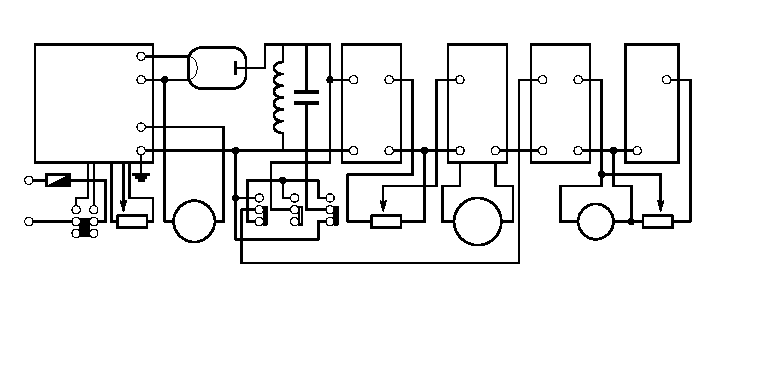
\includegraphics[width=\textwidth]{2_7_2}
	\caption{Блок-схема установки для измерения дробового шума. Внизу изображена
нижняя часть передней панели с ручками и кнопками управления}
	\figmark{exp Schottky noise}
\end{figure}

Сила анодного тока шумового диода в режиме насыщения определяется эмиссией 
(а значит, температурой) его катода. Анодный ток~$I_{\text{а}}$ измеряется 
миллиамперметром и регулируется потенциометром~$R_{\text{а}}$, ручка которого 
на панели прибора обозначена~<<$R_{\text{а}}$>>. Чувствительность измерительной 
схемы регулируется делителем напряжения~$R_{\text{д}}$, расположенным между 
усилителем и квадратичным детектором. Его ручка на панели 
обозначена~<<$R_{\text{д}}$>>. На выходе квадратичного детектора установлен
микроамперметр. Отклонение стрелки микроамперметра пропорционально квадрату
напряжения на входе детектора, поэтому он
пригоден для измерения переменных напряжений. Таким образом, показания
микроамперметра пропорциональны квадрату шумового
напряжения, причём коэффициент пропорциональности зависит от положения реостата
$R_{\text{д}}$ и, вообще говоря, неизвестен.
Поэтому при измерениях экспериментатор замечает показание микроамперметра, а
затем вместо сигнала с колебательного
контура подаёт на вход усилителя калибровочный сигнал с настроенного на ту же
частоту генератора. Этот сигнал измеряется
вольтметром (обозначение <<$U_{\text{г}}$>> на панели) и ослабляется в точно
известное число раз прецизионным аттенюатором. При
измерениях напряжение на генераторе подбирается так, чтобы стрелка
микроамперметра вернулась к отмеченному делению. В
этом случае напряжение шумов равно известному напряжению, подаваемому на
усилитель с аттенюатора. Делитель $R_{\text{д}}$ во
время этой процедуры, конечно, нельзя трогать.

Генератор используется не только для калибровки квадратичного детектора, но и
для измерения добротности контура.
Измерения производятся по методу $Q$-метра. Включим в контур генератор~Г
(настроенный на собственную частоту контура),
как это изображено на рис.~\figref{scheme Q}. Выходное напряжение генератора
$U_{\text{г}}$ целиком падает на активном сопротивлении контура $R$.
Поэтому $U_{\text{г}}=IR$, где $I$~--- ток в контуре. Найдём теперь напряжение
$U_{\text{к}}$, подаваемое на усилитель и измеряемое
квадратичным детектором:
\begin{equation*}
U_{\text{к}}=U_{\text{г}}-\frac{I}{i\omega
C}=U_{\text{г}}-\frac{U_{\text{г}}}{i\omega
RC}\approx\frac{iU_{\text{г}}}{\omega RC}.
\end{equation*}
При написании последнего равенства считалось, что контур обладает высокой
добротностью, $Q=1/\omega RC\gg1$. Заменяя $1/\omega
RC$ через добротность контура, найдём
\begin{equation}
	\eqmark{2.7.13}
	Q=\frac{|U_{\text{к}}|}{|U_{\text{г}}|}.
\end{equation}

\begin{figure}[h!]
    \centering\small
	\pic{0.6\textwidth}{Chapter_2/2_7_3}
	%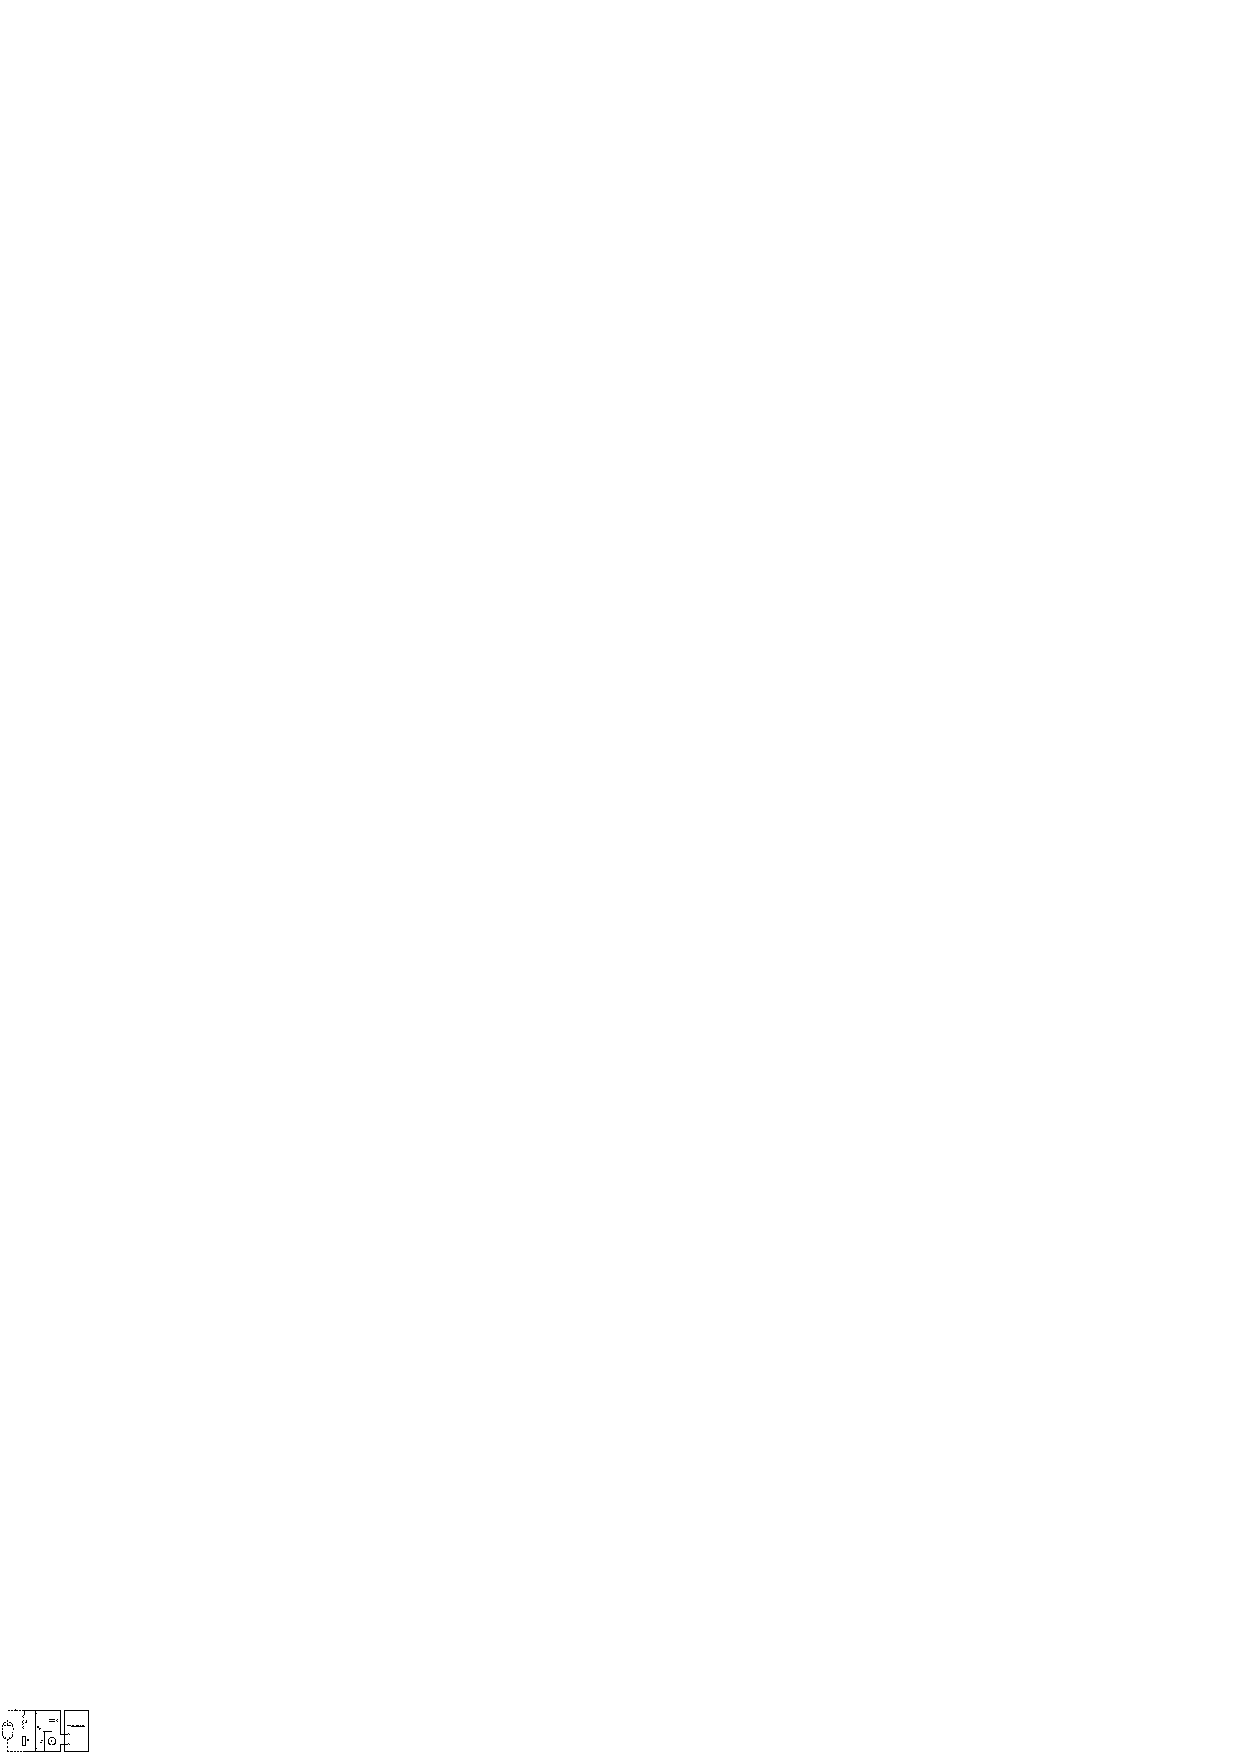
\includegraphics[width=\textwidth]{2_7_3}
	\caption{Схема для измерения добротности колебательного контура}
	\figmark{scheme Q}
\end{figure}

Итак, для измерения добротности контура нужно сравнить напряжение на генераторе
с напряжением на катушке самоиндукции.
Напряжение на генераторе $U_{\text{г}}$ измеряется вольтметром генератора
(рис.~\figref{exp Schottky noise}). Измерение напряжения на катушке самоиндукции
не так просто.

При измерении напряжения $U_{\text{к}}$, создаваемого генератором на катушке
самоиндукции, необходимо учитывать и шумовое
напряжение $U_{\text{ш}}$, имеющееся на катушке. Это напряжение при измерениях
продолжает возбуждаться диодом, так как при
измерениях добротности контура диод находится в рабочем режиме. Отключить диод
при измерении нельзя, поскольку
добротность контура от этого заметно изменится: при измерениях шума контур
шунтирован диодом, что снижает его
добротность; в этом положении и должна измеряться добротность контура. При
включении генератора в контур на вход
усилителя поступает не $U_{\text{к}}$, как показано на рис.~\figref{scheme Q}, и
не $U_{\text{ш}}$, а их сумма. При этом ток детектора $I_{\text{д}}$
пропорционален
$\langle (U_{\text{ш}}+U_{\text{к}})^2\rangle$. Сдвиг фаз между колебаниями
$U_{\text{ш}}$ и $U_{\text{к}}$ непрерывно изменяется. Поэтому
\begin{equation*}
I_{\text{д}}\propto\langle (U_{\text{ш}}+U_{\text{к}})^2\rangle=\langle
U_{\text{ш}}^2\rangle+2\langle U_{\text{ш}}U_{\text{к}}\rangle+\langle
U_{\text{к}}^2\rangle=\langle U_{\text{ш}}^2\rangle+\langle
U_{\text{к}}^2\rangle,
\end{equation*}
в то время как до включения генератора ток детектора $I_{\text{д}}$ был
пропорционален $U_{\text{ш}}^2$.

Таким образом, $U_{\text{к}}^2$ пропорционально \important{приращению} тока
квадратичного детектора, происходящему при включении
напряжения $U_{\text{г}}$. Чтобы подставить это приращение в формулу
\eqref{2.7.13}, оно должно быть пересчитано в напряжение
генератора. Это делается следующим образом. Нужно заметить показание
квадратичного детектора при нулевом напряжении на
выходе генератора. Затем нужно установить на выходе генератора некоторое
напряжение $U_{\text{г}}$ и зафиксировать приращение
тока детектора $\Delta I_{\text{д}}$, вызванное напряжением генератора. После
этого вместо колебательного контура на вход усилителя
следует подключить генератор с аттенюатором. Сигнал с генератора и положение
аттенюатора нужно подобрать таким образом,
чтобы показание микроамперметра было равно измеренному ранее приращению $\Delta
I_{\text{д}}$. Показание вольтметра генератора равно
искомому напряжению $U_{\text{к}}$.

%\todo[author=Tiffani]{Сделать нормальный рисунок. Этот даже не отображается}
\begin{figure}[h!]
    \centering\small
	\pic{0.85\textwidth}{Chapter_2/2_7_4}
	\caption{Схема установки для измерения напряжения шума}
	\figmark{scheme U noise}
\end{figure}

\begin{lab:task}
\taskpreamble{В работе предлагается, измерив напряжение шумов, раскачивающих колебательный
контур, и определив добротность этого
контура, рассчитать заряд электрона.}

\tasksection{Проверка квадратичности детектора}

	\item Включите питание стенда (кнопка <<Сеть>>).

	\item Убедитесь в том, что выпрямительная схема с полупроводниковыми диодами
действительно имеет квадратичную
характеристику. Для этого включите стенд в режим измерения напряжения генератора
(кнопка <<$U_{\text{г}}$>>). Установите
максимальную  чувствительность квадратичного детектора
(регулятор~$R_{\text{д}}$) и подберите предел измерений для вольтметра
(кнопка <<100>> или <<300>>~мкВ аттенюатора). Изменяя выходное напряжение
генератора с помощью регулятора напряжения генератора~$R_{г}$, 
измерьте зависимость тока квадратичного детектора~$I_{\text{д}}$ 
от входного напряжения усилителя~$U_{\text{г}}$.

\tasksection{Измерение напряжения шума}

	\item Включите режим измерения шума (кнопка <<$U_{ш}$>>).
Электрическая схема для этого случая показана на рис.~\figref{scheme U noise}.

	\item Установите анодный ток шумового диода $I_{а}=1$~мА, изменяя
регулятором $R_{А}$ напряжение накала диода.

С помощью регулятора $R_{д}$ подберите чувствительность квадратичного
детектора так, чтобы стрелка микроамперметра
отклонялась на б\'{о}льшую часть шкалы. Отметьте значение шумового
тока~$I_{д}$.

Для пересчёта отклика детектора на шум в единицы напряжения вместо шумового
диода подключите к усилителю генератор напряжений (кнопка~<<$U_{г}$>>).
Измерительная схема приведена на рис.~\figref{scheme U generator}.

С помощью регулятора $R_{г}$ и аттенюатора (пределы <<30>>, <<100>> или
<<300>>~мкВ) установите \important{то же значение тока} $I_{д}$,
которое было выбрано в режиме измерения шума. Регулятор~$R_{д}$ во время
этой процедуры, конечно, трогать нельзя. Отсчитанное по вольтметру
с аттенюатором напряжение~$U_{эфф}$ равно корню квадратному из среднего
квадрата напряжения шумов.

\begin{figure}[h!]
    \centering\small
    \pic{0.8\textwidth}{Chapter_2/2_7_5}
    \caption{Схема установки для измерения напряжения на генераторе}
    \figmark{scheme U generator}
\end{figure}

\tasksection{Измерение добротности контура}

	\item При том же анодном токе диода переключите аттенюатор в положение <<1>>
или <<3>>~мкВ. Установите режим измерения
напряжения на контуре при его последовательном возбуждении
(кнопка~<<$U_{\text{к}}$>>). При нулевом напряжении на вольтметре
подберите чувствительность детектора: регулятором $R_{\text{д}}$ установите
стрелку микроамперметра детектора на любое целое
деление. Измерьте \important{приращение} тока детектора $\Delta I_{\text{д}}$
при изменении напряжения генератора от нуля до любого
напряжения~$V_1$.

Затем включите режим измерения напряжения на генераторе
(кнопка~<<$U_{\text{г}}$>>) и регулятором $R_{\text{г}}$ подберите напряжение
$V_2$, при котором ток квадратичного детектора равен \important{приращению}
$\Delta I_{\text{д}}$ в режиме измерения сигнала с~контура.
Добротность контура равна $Q=V_2/V_1$.

	\item Повторите измерения п.~2--3 ещё 5--6 раз при том же
анодном токе (можно при другой чувствительности детектора).

	\item Проведите измерения п.~2--4 при других значениях анодного
тока в интервале 1--4~мА.

	\item Запишите значения ёмкости и резонансной частоты колебательного
контура, указанные на установке.

\tasksection{Обработка результатов}

	\item Постройте график зависимости $I_{\text{д}}=f(U^2_{\text{г}})$ для
проверки характера детектирования.

	\item Вычислите среднюю величину заряда электрона для каждого значения тока
анода. Представьте результаты в виде таблицы.

%\bigskip
\begin{center}
\begin{tabular}{|c|c|c|c|c|}
\hline $\;I_{\text{а}}$,~мА&$\;U_{\text{эфф}}$,~мкВ&$\quad\langle
Q\rangle\quad$&$e~$, Кл&$\langle e\rangle\pm\Delta e$\\\hline
 & & & &\\
 & & & &\\
\hline
\end{tabular}
\end{center}

	\item Определите заряд электрона, используя все полученные результаты, и
оцените погрешность. Сравните полученное значение
с табличным.
\end{lab:task}

%\todo[author=Tiffani]{Нет вопросов к лабораторной.}

\begin{lab:literature}
	\item \emph{Власов~В.Ф.} Электронные и ионные приборы.~--- М.:~Связьиздат,
1960, \S~13.5.

	\item \emph{Рытов~С.М.} Введение в статистическую радиофизику.~---
М.:~Наука, 1976, \S~5.
\end{lab:literature}

\lab{Релаксационные колебания}

\aim{изучение вольт-амперной характеристики нормального тлеющего разряда;
исследование релаксационного генератора на стабилитроне.}

\equip{стабилитрон СГ-2 (газонаполненный диод) на монтажной панели, амперметр,
вольтметр, магазин сопротивлений, магазин ёмкостей, источник питания,
осциллограф (ЭО), генератор звуковой частоты (ЗГ).}

Перед выполнением работы необходимо ознакомиться с п.~\ref{sec:auto} Введения
к разделу.

Колебательные системы, как правило, имеют два накопителя энергии, между
которыми происходит её перекачка. Например, в контуре,
содержащем конденсатор и катушку индуктивности, электрическая энергия переходит
в магнитную и обратно.
Встречаются, однако, колебательные системы, содержащие всего один накопитель
энергии. Рассмотрим в качестве примера
электрическую цепь, содержащую конденсатор и сопротивление без самоиндукции.
Разряд конденсатора через сопротивление
представляет собой апериодический процесс. Разряду, однако, можно придать
периодический характер, возобновляя заряд
конденсатора через постоянные промежутки времени. Колебания в этом случае
являются совокупностью двух апериодических
процессов~--- процесса зарядки конденсатора и процесса его разрядки. Такие
колебания называются \term{релаксационными}.


В данной работе роль <<ключа>>, обеспечивающего попеременную зарядку и
разрядку конденсатора, играет газоразрядный диод. 
Зависимость тока от напряжения для газоразрядной лампы не подчиняется
закону Ома и характеризуется рядом
особенностей (рис.~\figref{VACH stabilitron}). При малых напряжениях лампа
практически не пропускает тока (участок OAB на рис.~\figref{VACH stabilitron}).
Ток в лампе возникает только в том случае, если разность потенциалов на её
электродах достигает \important{напряжения зажигания}~$U_1$. 
При этом скачком (участок BC) устанавливается конечная сила тока~$I_1$~--- в лампе возникает
\important{нормальный тлеющий разряд} (см. подробнее Приложение к Разделу~V,
стр.~\pageref{sec:discharge}). 
При дальнейшем незначительном увеличении напряжения сила тока заметно возрастает 
по закону, близкому к линейному (участок CD). Нормальный тлеющий разряд~---
стабилизатор напряжения, отсюда второе название лампы~--- \important{стабиловольт}.


Если начать уменьшать напряжение на горящей лампе, то при напряжении, равном
$U_1$, лампа ещё не гаснет, и сила тока
продолжает уменьшаться (участок CE на рис.~\figref{VACH stabilitron}). 
Лампа перестанет пропускать ток лишь при \important{напряжении гашения}~$U_2$, 
которое обычно
существенно меньше $U_1$. Сила тока при этом скачком падает от значения~$I_2$
($I_2<I_1$) до нуля (участок EA).

\begin{figure}[h!]
    \centering
    \pic{0.4\textwidth}{Chapter_2/5_1_1}
    \caption{Вольт-амперная характеристика стабилитрона с последовательно
        включённым резистором}
    \figmark{VACH stabilitron}
\end{figure}
%\rpic{38mm}{5_1_1}{\cct Вольт-амперная характеристика стабилитрона с
%последовательно включённым резистором}{1}

Характеристика, изображённая на рис.~\figref{VACH stabilitron}, несколько
идеализирована. У~реальной лампы зависимость~$I(U)$ не вполне линейна.
При $U>U_1$ графики, соответствующие возрастанию и убыванию напряжения, 
могут не совпадать. Эти отличия, впрочем, носят второстепенный характер 
и для нашей задачи несущественны.


Рассмотрим схему релаксационного генератора, представленную
на рис.~\figref{generator scheme}. Пусть напряжение батареи $\mathcal{E}$ больше
напряжения зажигания $U_1$. В обозначениях, принятых на схеме, справедливо уравнение
\begin{equation*}
I_C+I(U)=\frac{\mathcal{E}-U}{R}
\end{equation*}
или
\begin{equation}
	\eqmark{2.8.1}
	C\frac{dU}{dt}+I(U)=\frac{\mathcal{E}-U}{R}.
\end{equation}
В стационарном режиме работы, когда напряжение $U$ на конденсаторе постоянно и
$dU/dt = 0$, ток через лампу равен
\begin{equation}
	\eqmark{2.8.2}
	I_{\text{ст}}=\frac{\mathcal{E}-U}{R}.
\end{equation}

\begin{figure}[h!]
    \centering
    \pic{0.4\textwidth}{Chapter_2/5_1_2}
    \caption{Принципиальная схема релаксационного генератора}
    \figmark{generator scheme}
\end{figure}
%\rpic{4.0cm}{5_1_2}{\cct Принципиальная схема релаксационного генератора}{2}

Равенство \eqref{2.8.2} может быть представлено графически
(рис.~\figref{generator work}).
При разных $R$ графики имеют вид прямых, пересекающихся в точке $U=\mathcal{E}$,\\*$I=0$.
Область, где эти \important{нагрузочные прямые}
пересекают вольт-амперную характеристику лампы, соответствует стационарному
режиму~---~при малых $R$ (прямая~1) лампа
горит постоянно, колебания отсутствуют. Прямая~2, проходящая через точку
($I_2$,~$U_2$), соответствует критическому
сопротивлению
\begin{equation}
	\eqmark{2.8.3}
	R_{\text{кр}}= \frac{\mathcal{E}-U_2}{I_2}.
\end{equation}
При сопротивлении $R>R_{\text{кр}}$ нагрузочная прямая~3 не пересекает
характеристику лампы, поэтому стационарный режим
невозможен. В этом случае в системе устанавливаются колебания.

\begin{figure}[h!]
    \centering
    \pic{0.4\textwidth}{Chapter_2/5_1_3}
    \caption{Режимы работы релаксационного генератора}
    \figmark{generator work}
\end{figure}
%\rpic[14]{4.0cm}{5_1_3}{\cct Режимы работы релаксационного генератора}{3}

Рассмотрим, как происходит колебательный процесс. Пусть в начале опыта ключ~К
разомкнут (рис.~\figref{generator scheme}) и $U=0$. Замкнём ключ.
Конденсатор~$C$ начинает заряжаться через сопротивление~$R$, напряжение на нём
увеличивается (рис.~\figref{relax osc}). Как только оно
достигнет напряжения зажигания $U_1$, лампа начинает проводить ток, причём
прохождение тока сопровождается разрядкой
конденсатора. В самом деле, батарея~$\mathcal{E}$, подключённая через большое
сопротивление~$R$, не может поддерживать необходимую
для горения лампы величину тока. Во время горения лампы конденсатор разряжается,
и когда напряжение на нём достигнет
потенциала гашения, лампа перестанет проводить ток, а конденсатор вновь начнёт
заряжаться. Возникают релаксационные
колебания с~амплитудой, равной $(U_1-U_2)$.

\begin{figure}[h!]
    \centering
	\pic{0.8\textwidth}{Chapter_2/5_1_4}
	\caption{Осциллограмма релаксационных колебаний}
	\figmark{relax osc}
\end{figure}
%\rpic{5.0cm}{5_1_4}{\cct Осциллограмма релаксационных колебаний}{4}

Рассчитаем период колебаний. Полное время одного периода колебаний $T$ состоит
из суммы времени зарядки $\tau_{\text{з}}$ и
времени разрядки $\tau_{\text{р}}$, но если сопротивление $R$ существенно
превосходит сопротивление зажжённой лампы, то
$\tau_{\text{з}}\gg \tau_{\text{р}}$ и $T\approx\tau_{\text{з}}$ (этим случаем
мы и ограничимся).

Во время зарядки конденсатора лампа не горит ($I(U)=0$), и уравнение
\eqref{2.8.1} приобретает вид
\begin{equation}
	\eqmark{2.8.4}
	RC\frac{dU}{dt}=\mathcal{E}-U.
\end{equation}
Будем отсчитывать время с момента гашения лампы, так что $U=U_2$ при $t=0$
(рис.~\figref{relax osc}). Решив уравнение \eqref{2.8.4}, найдём
\begin{equation}
	\eqmark{2.8.5}
	U=\mathcal{E}-(\mathcal{E}-U_2)e^{-t/RC}.
\end{equation}
В момент зажигания $t=\tau_{\text{з}}$, $U=U_1$, поэтому
\begin{equation}
	\eqmark{2.8.6}
	U_1=\mathcal{E}-(\mathcal{E}-U_2)e^{-\tau_{\text{з}}/RC}.
\end{equation}
Из уравнений \eqref{2.8.5} и \eqref{2.8.6} нетрудно найти период колебаний:
\begin{equation}
	\eqmark{2.8.7}
	T\approx \tau_{\text{з}}=RC\ln\frac{\mathcal{E}-U_2}{\mathcal{E}-U_1}.
\end{equation}

Развитая выше теория является приближённой. Ряд принятых при расчётах упрощающих
предположений оговорен в тексте.
Следует иметь в виду, что мы полностью пренебрегли паразитными емкостями и
индуктивностями схемы. Не рассматривались
также процессы развития разряда и деионизация при гашении. Поэтому теория
справедлива лишь в тех случаях, когда в схеме
установлена достаточно большая ёмкость и когда период колебаний существенно
больше времени развития разряда и времени
деионизации (практически $\gg10^{-5}$~с). 
Кроме того, потенциал гашения $U_2$, взятый из статической вольт-амперной
характеристики, может отличаться от потенциала гашения лампы, работающей в
динамическом режиме релаксационных колебаний.

\begin{lab:task}

\taskpreamble{В работе предлагается получить вольт-амперную характеристику
стабилитрона и познакомиться с работой релаксационного генератора: определить
критическое сопротивление, исследовать зависимость периода колебаний от
сопротивления при фиксированной ёмкости и от ёмкости при фиксированном
сопротивлении.}

\tasksection{Измерение ВАХ стабилитрона}

		\item Соберите схему, изображённую на рис.~\figref{stabilitron scheme
charact}. Добавочное сопротивление~$r$ подпаяно между ножкой лампы и
соответствующей клеммой для того, чтобы предохранить стабилитрон от перегорания. 
Это сопротивление остаётся включённым при всех
измерениях. Запишите величину~$r$, указанную на установке.

\begin{figure}[h!]
    \centering
    \pic{0.45\textwidth}{Chapter_2/5_1_5} % закоммент. т.к. не работает
    \caption{Схема установки для~изучения характеристик стабилитрона}
    \figmark{stabilitron scheme charact}
\end{figure}
%\rpic{5.0cm}{5_1_5}{\cct Схема установки для~изучения характеристик
%стабилитрона}{5}

		\item Установите регулятор источника питания на минимум напряжения и
включите источник в сеть.

		\item Снимите вольт-амперную характеристику стабилитрона с
сопротивлением $r$ при возрастании и убывании напряжения. При
этом как можно точнее определите потенциалы зажигания и гашения $U_1$ и $U_2$ и
соответствующие токи $I_1$ и $I_2$.

\tasksection{Осциллограммы релаксационных колебаний}

		\item Соберите релаксационный генератор согласно
         рис.~\figref{scheme exp osc}.

		\item Установите на магазине ёмкостей значение $C=0,05$~мкФ, а на
магазине сопротивлений $R=900$~кОм.

		\item Включите в сеть осциллограф, звуковой генератор и источник питания
и установите напряжение $\mathcal{E}\approx 1,2\,U_1$.

\begin{figure}[h!]
    \centering
	\pic{0.9\textwidth}{Chapter_2/5_1_6}
	\caption{Схема установки для исследования релаксационных колебаний}
	\figmark{scheme exp osc}
\end{figure}
%\fcpic[1]{5_1_6}{Схема установки для исследования релаксационных колебаний}{6}

		\item Подберите частоту развёртки ЭО, при которой на экране видна
картина пилообразных колебаний (рис.~\figref{relax osc}).

		\item Получив пилу на экране, оцените соотношение между временем
зарядки~$\tau_{\text{з}}$ и временем разрядки $\tau_{\text{р}}$.
Зарисуйте картину колебаний.

		\item Уменьшая сопротивление магазина, определите $R_{\text{кр}}$, при
котором пропадают колебания, и сравните его с величиной,
рассчитанной по формуле~\eqref{2.8.3}. Это сравнение полезно сделать в процессе
работы и подумать о причинах расхождения
результатов.

Убедитесь, что колебания пропадают не только при уменьшении $R$ при постоянном
$\mathcal{E}$, но и при увеличении $\mathcal{E}$ при
постоянном $R$, когда это $R$ не слишком превышает $R_{\text{кр}}$.

\tasksection{Фигуры Лиссажу и частота колебаний}

		\item Восстановите исходные параметры релаксационного
генератора: $C=5\cdot 10^{-2}$~мкФ, $R=900$~кОм, $\mathcal{E}\approx 1,2 \cdot
U_1$. Подайте сигнал с генератора на вход $X$ осциллографа. Меняя частоту ЗГ,
получите на экране фигуру Лиссажу без
самопересечений, соответствующую отношению частот 1:1.

		\item Не меняя параметров релаксационного генератора, уменьшите частоту
ЗГ вдвое (втрое) и получите фигуры Лиссажу при
соотношении частот 2:1 (3:1). Зарисуйте эти кривые в тетрадь.

Получите и зарисуйте фигуры Лиссажу при увеличении частоты ЗГ в два и три раза
(1:2 и 1:3).

		\item При любом целом значении $R$ из интервала (2~--~4)~$R_{\text{кр}}$
снимите с помощью фигур Лиссажу 1:1 зависимость частоты
колебаний $\nu$ от ёмкости~$C$, меняя величину ёмкости в пределах от
$5\cdot10^{-2}$ до $5\cdot10^{-3}$~мкФ.

Напряжение $\mathcal{E}$, необходимое для расчёта теоретического значения периода по
формуле \eqref{2.8.7}, следует поддерживать
постоянным.

		\item Проведите серию измерений $\nu(R)$ при постоянной ёмкости 
$C=5\cdot10^{-2}$, меняя величину $R$ от максимального
значения до критического.

\tasksection{Обработка результатов}

		\item Постройте графики вольт-амперных характеристик~$I(U)$ для системы, 
        состоящей из стабилитрона и дополнительного сопротивления $r$ 
        (по результатам измерений) и 
        для стабилитрона без сопротивления~$r$ (вычитая падение напряжения
на сопротивлении~$r$ при каждом токе).
Сравните относительные изменения тока и напряжения на стабилитроне.

		\item Рассчитав экспериментальные и теоретические значения периодов,
постройте графики $T_{\text{эксп}}(C)$ и $T_{\text{теор}}(C)$ на
одном листе. На другом листе постройте графики $T_{\text{эксп}}(R)$ и~$T_{\text{теор}}(R)$.

		\item Если наклоны теоретической и экспериментальной прямых заметно
отличаются, рассчитайте из экспериментальной прямой
динамический потенциал гашения. Потенциалы зажигания можно считать одинаковыми.
\end{lab:task}


\begin{lab:questions}
	\item Какие колебания называются релаксационными?

	\item От каких параметров газа зависит напряжение зажигания стабиловольта?

	\item Почему напряжение гашения существенно меньше напряжения зажигания?

%	\item Какие режимы работы релаксационного генератора Вы знаете?

	\item Как по вольт-амперной характеристике стабиловольта и известным
параметрам генератора найти ток в лампе в стационарном
режиме?

	\item Что такое критическое сопротивление релаксационного генератора? От
чего оно зависит?

	\item Почему критическое сопротивление зависит от величины напряжения $\mathcal{E}$ на
входе генератора? Рассмотрите рис.~\figref{generator work}.

	\item Почему при малой ёмкости колебания не возникают (лампа не гаснет) даже
при $R>R_{\text{кр}}$? Оцените <<малость>> ёмкости,
сравнив время релаксации и время деионизации.
\end{lab:questions}


\begin{lab:literature}

	\item \SivuhinIII~--- \S~134.

	\item \Kalashnikov~--- \S~244.

	\item \emph{Горелик~Г.С.} Колебания и волны.~--- М.:~Физматгиз, 1959.
Гл.~IV, \S~6.
\end{lab:literature}

\lab{Электромагнитные волны в волноводе}
\todo[author=Tiffani]{Номер лабораторной?}
\todo[author=Tiffani]{Необходимо сделать рисунки во всю лабораторную}
\begin{lab:aim}
ознакомление с особенностями распространения электромагнитных волн в волноводе, аппаратурой и методами измерения основных характеристик протекающих при этом процессов.
\end{lab:aim}

\begin{lab:equipment}
генератор сигналов сверхвысокой частоты, измерительная линия, усилитель, заглушка, отрезок волновода с поглощающей нагрузкой, отрезки волноводов различных сечений, детекторная головка.
\end{lab:equipment}

Передача энергии электромагнитных колебаний низкой частоты, например, 50~Гц, не представляет проблем и делается широко известным способом: по проводам. На более высоких частотах (до 300~МГц) эта задача решается с помощью двухпроводных линий и коаксиальных кабелей. На ещё более высоких частотах (до 300~ГГц) при колебаниях с длинами волн (в вакууме) от 1~метра до 1~миллиметра (этот диапазон называется \important{диапазоном сверхвысоких частот} или, сокращённо, СВЧ) передача энергии с помощью двухпроводной линии или коаксиальных кабелей становится малоэффективной из-за больших потерь: резко возрастает сопротивление проводов из-за \important{скин-эффекта}~---~вытеснения тока на поверхность, а в двухпроводной линии, кроме того, потери растут вследствие излучения энергии в окружающее пространство.

В СВЧ-диапазоне энергия передаётся с помощью металлических труб, называемых волноводами (в миллиметровом диапазоне длин волн волноводы могут быть сделаны и из диэлектрика). Электромагнитные волны могут распространяться по металлическим трубам любого профиля, но из технологических соображений сечения волноводов делаются либо круглыми, либо прямоугольными.

Чтобы найти структуру электромагнитного поля в волноводе, надо решить уравнения Максвелла с соответствующими граничными условиями. Решение этой задачи приведено во многих учебниках.

Для радиоволн, бегущих по волноводу вдоль оси $Z$ с проводящими стенками, расположенными на расстоянии $a$ друг от друга (простейший волновод), с вектором напряженности электрического поля $\vec E=E_y \vec e_y,$ перпендикулярным плоскости $ZX$. Такое решение может быть записано в виде:
\begin{equation}
	\eqmark{2.0.1}
	E_y=A\sin\left(\dfrac{n\pi x}{a}\right)\sin(\omega t-k_zz), \qquad n=0,~1,~2,~3 \ldots,
\end{equation}
где $k_z=\sqrt{k^2-k^2_x}, k=2\pi/\lambda_0=\omega/c, \lambda_0$~---~длина волны в вакууме, $\omega=2\pi f$, $f$~---~частота генератора, $c$~---~скорость света. Множитель $\sin\left(\dfrac{n\pi x}{a}\right)$ физически соответствует стоячей волне между стенками волновода по координате $Х$ и определяет граничные условия $E_y=0$ на проводящих стенках.
	
\begin{figure}[h!]
	%\centering\includegraphics[width=0.6\linewidth]{Chapter_2/13}
	\caption{Волновод и примеры распределения поля}
	\figmark{waveguide}
\end{figure}
	
Для бегущих вдоль волновода волн $k_z$~---~действительная величина. Предельный случай $k_z=0$ соответствует $k=k_x,$ что при условии $n=1$ приводит к формулам для \important{критических длины и циклической частоты волн}, распространяющихся в вакуумном волноводе:
\begin{equation}
	\eqmark{2.0.2}
	\lambda_{\text{кр}}=2a, \qquad \omega_{\text{кр}}=\pi c/a.
\end{equation}
Если $\lambda>2a$ и, соответственно, $\omega<\pi c/a,$ то электромагнитная волна при распространении вдоль волновода затухает.

Для бегущей волны фазовая скорость 
\begin{equation}
	\eqmark{2.0.3}
	V_{\text{Ф}}=\omega/k_z=c/\sqrt{1-\omega^2_{\text{кр}}/\omega^2}
\end{equation}
больше скорости света в вакууме $c,$ а длина волны в волноводе
\begin{equation}
	\eqmark{2.0.4}
	\lambda_{\text{В}}=\lambda_0/\sqrt{1-(\lambda_0/2a)^2}
\end{equation}
больше длины волны в вакууме $\lambda_0.$
В представленном на рис.~\figref{waveguide} случае отлична от нуля продольная составляющая магнитного поля, и такую волну называют \important{магнитной ($H$-волна).} Обычно для передачи СВЧ-энергии по прямоугольному волноводу используется волна (мода) $H_{10}.$  Второй индекс $0$ соответствует отсутствию составляющей электромагнитного поля $E_x.$ Критическая длина волны моды $H_{10}$~---~максимальная среди всех типов волн в прямоугольном волноводе, и поэтому ее называют \important{основной.} Тем самым, для волновода заданного сечения существует диапазон частот, ограниченный снизу критической частотой волны $H_{10}$ ($\lambda_{\text{кр}}=2a$). Следующая по возрастанию частоты~---~мода $H_{01}$ с $\lambda_{\text{кр}}=2b$ или $H_{20}$ с $\lambda_{\text{кр}}=a,$ если $a>b.$

В заданном частотном диапазоне СВЧ-энергия может переноситься одним типом волн, что существенно облегчает её дальнейшее использование.

Если в волноводе имеется какое-либо препятствие, нерегулярность, то в нём появляется \important{отражённая волна.} Падающая $E_0$ и отраженная волна с коэффициентом отражения $\rho$ по амплитуде интерферируют и создают в волноводе стоячую волну.

Максимальное (в пучности) и минимальное (в узле) значения поля равны соответственно
\begin{equation}
	\eqmark{2.0.5}
	E_{\text{max}}=E_0(1+\rho), \qquad E_{\text{min}}=E_0(1-\rho).
\end{equation}
Отношение $K=E_{\text{max}}/E_{\text{min}}$ называется \important{коэффициентом стоячей волны} (к.с.в.). Коэффициент отражения от препятствия по амплитуде
\begin{equation}
	\eqmark{2.0.6}
	\rho=\dfrac{E_{\text{max}}-E_{\text{min}}}{E_{\text{max}}+E_{\text{min}}}=\dfrac{K-1}{K+1}.
\end{equation}

В случае полного отражения (металлическая заглушка) $\rho=1,$ а если в волновод вставлено вещество, поглощающее СВЧ-­излучение (согласованная нагрузка), то $\rho=0.$

Для определения коэффициента стоячей волны обычно используют измерительную линию~---~отрезок волновода с продольной щелью длиной в несколько полуволн. В щели располагается зонд~---~большой металлический штырь (антенна), реагирующий на электрическое поле в волноводе. Напряжение высокой частоты, наводимое на зонд, детектируется, усиливается и подаётся на микровольтметр. Зонд может перемещаться вдоль линии, что позволяет исследовать распределение электрического поля в волноводе.

\labsection{А. Волны в волноводе при частоте выше критической}

\experiment
Схема для исследования структуры волн в волноводе при частоте выше критической представлена на рис.~\figref{scheme microwave}. Модулированный сигнал от высокочастотного генератора (цуги с частотой повторения 1~кГц) поступает на вход измерительной линии, вдоль которой перемешается зонд~8. Высокочастотный сигнал с зонда поступает на кристаллический детектор $D$.

\begin{figure}[h!]
	%\centering\includegraphics[width=0.6\linewidth]{Chapter_2/13}
	\caption{Схема для исследования структуры волн СВЧ}
	\figmark{scheme microwave}
\end{figure}

С нагрузки детектора (с $RС$-цепочки) снимается огибающая высокочастотного сигнала и подаётся на усилитель низкой частоты. Величина сигнала регистрируется вольтметром, вмонтированным в усилитель. Ручка~$С$~---~настройка измерительной линии~--- служит для согласования зонда (как антенны) со входом усилителя. Как правило, они согласованы, и в настройке нет необходимости. В волноводе с закрытым выходом образуется стоячая волна. Определив расстояние между узлами, можно рассчитать длину волны и фазовую скорость СВЧ-сигнала в волноводе. Устройство детекторной головки, установленной на измерительной линии, таково, что отклик вольтметра $U$ на величину напряжённости электрического поля $Е$ в волноводе 
\begin{equation*}
	U\sim E^{n},
\end{equation*}
а показатель степени $n$ сам зависит от величины сигнала: при малых сигналах детектирование квадратичное $(n=2),$ при больших~---~линейное $(n=1).$

Меняя нагрузку на выходе измерительной линии (ручка~$B$ на рис.~\figref{scheme microwave}) и сравнивая максимальное и минимальное показания вольтметра, можно рассчитать коэффициент стоячей волны $K$ и коэффициент отражения $\rho.$

\labsection{Б. Волны в волноводе при частоте ниже критической}

Для исследования затухания волн в волноводе при частоте ниже критической используются те же генератор, усилитель, измерительная линия и дополнительный набор волноводов с отдельной детекторной головкой $G$ (рис.~\figref{scheme damping}). Дополнительный набор начинается и заканчивается волноводами переменного сечения I и II. Между ними

\begin{figure}[h!]
	%\centering\includegraphics[width=0.6\linewidth]{Chapter_2/13}
	\caption{Схема для исследования затухания}
	\figmark{scheme damping}
\end{figure}

можно разместить 1,~2 или 3 одинаковых отрезка с постоянным сечением. В такой системе волны с частотами меньше критической экспоненциально затухают.

Мощность сигнала на выходе из волновода $W$ можно связать с мощностью входного сигнала $W_0$ двумя способами: $W=W_0e^{-\alpha z}$ или $W=W_0~10^{-\beta z},$ где $z$~---~длина волновода. Величина $(\alpha z)$ измеряется в Неперах (Нп): один Непер соответствует отношению интенсивностей, равному основанию натуральных логарифмов. Величину $(\beta z)$ принято измерять в децибелах (дБ): один Бел соответствует уменьшению мощности в 10 раз; децибел~---~одна десятая Бела. Измеренное в децибелах затухание определяется формулой $\beta z(\text{дБ})=10\times\lg(W_0/W).$ Отсюда следует, что $\alpha(\text{Нп})=2,3\beta(\text{Б}).$

Если при уменьшении количества вставок волновода поддерживать интенсивность выходного сигнала постоянной, то входной сигнал следует ослабить. Степень ослабления $\gamma$ зависит от длины волновода $z~(\gamma~=~\beta~z)$ и измеряется по шкале генератора в децибелах. Именно таким образом в эксперименте определяется коэффициент затухания $\beta.$ Его можно сравнить с коэффициентом $\alpha,$ рассчитанным теоретически. В закритическом волноводе при квадратичном детектировании интенсивность сигнала падает по закону $E^2\sim e^{-\alpha z},$ где $\alpha$~---~коэффициент затухания:
\begin{equation}
	\eqmark{2.0.7}
	\alpha=2ik_{Z}=\dfrac{2\omega}{c}\sqrt{\left(\dfrac{\omega_{kp}}{\omega}\right)^2-1}=\dfrac{2\pi}{a}\sqrt{1-\left(\dfrac{2a}{\lambda_0}\right)^2}.
\end{equation}
Здесь $\lambda_0=c/f=3,22$~см – длина волны в свободном пространстве, соответствующая рабочей частоте $f=9320$~МГц, $a=1,6$~см~---~размер широкой стенки волновода-вставки.

\begin{lab:task}

В работе предлагается при частоте выше критической исследовать стоячую волну в измерительной линии (рис.~\figref{scheme microwave}): измерив распределение сигнала вдоль волновода, рассчитать фазовую скорость; затем, меняя нагрузку на выходе волновода (заглушка, открытый конец или поглотитель), определить коэффициенты отражения волн $\rho.$ При частоте ниже критической предлагается определить коэффициент затухания волны $\beta$ в сборном волноводе (рис.~\figref{scheme damping}) и сравнить с его теоретическим значением.

	\tasksection{А. Исследование структуры волн при частоте выше 
		критической}

Мощность сигнала, снимаемого с генератора Г4-83, невелика, поэтому излучение не представляет опасности для здоровья человека. Тем не менее, заглядывать в открытый волновод при включённом генераторе не рекомендуется.

\begin{enumerate}
	\tasksection{I. Определение длины волны СВЧ-сигнала в волноводе}

	\item Проведите подготовку приборов к работе по техническому описанию (ТО), лежащему на рабочем столе.
	
	\item Установите рабочую частоту $f=9320$~МГц; перемещая зонд, настройтесь на пучность стоячей волны. Если при этом показания вольтметра превышают 1~мВ, следует ослабить сигнал, идущий от генератора, с помощью аттенюатора~4 (при напряжениях $\ge1$~мВ меняется характер детектирования).
	
	\item С помощью переключателей~5 и 9 подберите чувствительность вольтметра так, чтобы в максимуме стрелка отклонялась почти на всю шкалу. Используя весь возможный диапазон перемещения зонда вдоль измерительной линии, снимите зависимость показаний вольтметра $U$ от положения зонда $z$ (100 делений винта у выхода измерительной линии соответствуют 1~мм). Менять чувствительность вольтметра в течение этой серии нецелесообразно.
	
	\item Постройте график $U(z)$ и определите по нему длину волны $\lambda_{\text{В}}$ в волноводе. Сравните результат с теоретическим расчётом. Рассчитайте фазовую скорость $V_{\text{Ф}}$ волн в волноводе по формуле \eqref{2.0.3}. Рассчитайте групповую скорость $u,$ используя соотношение $uV_{\text{Ф}}=c^2.$	

	\tasksection{II. Определение коэффициентов отражения}

    \item Снимите металлическую заглушку с фланца измерительной линии. Перемещая зонд, измерьте максимальное ($U_{\text{max}}<1$~мВ) и минимальное напряжения в волне.
    
   \item Наденьте на выходной фланец измерительной линии отрезок волновода с поглощающей нагрузкой и снова измерьте максимальное и минимальное напряжения.
   
   \item Считая детектирование квадратичным, определите коэффициенты отражения $\rho$ для открытого и закрытого волновода и для волновода с поглощающей нагрузкой. Объясните полученные результаты. 

\tasksection{Б. Исследование затухания волн при частоте ниже
  		критической}
   
	\item Соберите схему согласно рис.~\figref{scheme damping} и настройте её по техническому описанию (ТО).
  
  \item Измерьте длину каждой волноводной секции.
  
  \item Рассчитайте критическую частоту для этого волновода ($f_{\text{кр}}=c/2a$, $a=1,6$~см) и убедитесь, что рабочая частота $f=9320$~МГц меньше критической.

	\tasksection{III. Измерение коэффициента затухания}

   \item Настройте детекторную головку на максимальную чувствительность согласно ТО, расположенному на установке (в этом упражнении ограничение $U<1$~мВ необязательно). Установите минимальное затухание ($\gamma=20$~дБ) сигнала от генератора и подберите чувствительность вольтметра так, чтобы стрелка отклонялась почти на всю шкалу; зарегистрируйте величины $U$ и $\gamma.$
   
   \item Последовательно уменьшая число промежуточных секций от трёх до нуля, каждый раз подбирайте такое ослабление сигнала от генератора, при котором показания вольтметра усилителя остаются неизменными.
   
  \item Постройте график в функции $\gamma=f(z),$ где $z$~---~полная длина подключенных волноводных секций. По наклону прямой рассчитайте коэффициент затухания $\beta=\Delta\gamma/\Delta z$ в единицах $\text{Б}/\text{см}$ и сравните с таким же коэффициентом, рассчитанным теоретически.
	\end{enumerate}
\end{lab:task}

\begin{lab:questions}

	\item Используя выражения для фазовой и групповой скоростей: $V_{\text{Ф}}=\omega/k$, $u=d\omega/dk,$~--- покажите, что в волноводе выполняется соотношение $uV_{\text{Ф}}=c^2.$
	
	\item Как направлен вектор Пойнтинга в волноводе?
\end{lab:questions}

\begin{lab:literature}

	\item \emph{Сивухин~Д.В.} Общий курс физики. – Т.~III, Электричество. – М.:~Физматлит, 2006, §§~139,~140.
	
	\item \emph{Кингсепп~А.С., Локшин~Г.Р., Ольхов~О.А.} Основы физики. Т.~1. – М.:~Физматлит, 2001, §~6.7.
	
	\item Фейнмановские лекции по физике. Т.~6. Электродинамика. – М.:~Наука, 1966, гл.~24.
	
\end{lab:literature}

\cleardoublepage
\chapter{Носители электрического тока}

Электрический ток представляет собой направленный перенос зарядов. Микрочастицы,
осуществляющие этот перенос, называют \mbox{\term{носителями тока}}. В конце
XIX века в опытах Дж.~Дж.~Томсона с <<катодными лучами>> были открыты
элементарные носители заряда~--- \term{электроны}. Вскоре были проведены
первые измерения величины элементарного заряда: Р.~Милликен
в опытах в 1908\,--\,1916 годов измерял заряд микроскопических капелек масла,
помещённых во внешнее электрическое поле. Идея этих опытов проста:
если элементарный заряд действительно существует, то величина заряда~$q$
любого тела может принимать только дискретную последовательность значений.
Сравнивая между собой заряды капель, можно убедиться в том, что все они
кратны одному и тому же числу~--- элементарному заряду~$e$:
\begin{equation*}
    q = 0,\,\pm e,\,\pm2e,\,\pm3e,\, \ldots
\end{equation*}
Величина заряда оказалась равной
\[
e\approx1,6\cdot 10^{-19}~Кл\qquad (e\approx 4,8\cdot 10^{-10}~ед.~СГС).
\]
Сразу после этого по отклонению <<катодных лучей>> в магнитном поле была
измерена и масса электрона $m_e\approx 9,1\cdot 10^{-31}$~кг.

Направленное движение зарядов в пространстве характеризуется 
\term{плотностью тока}:
\begin{equation}
\vec{j} = q n \vec{u},
\end{equation}
где $n$ --- объёмная концентрация носителей, $\vec{u}$ --- направленная составляющая 
средней скорости их движения~--- \term{дрейфовая скорость} (хаотическое тепловое
движение носителей вклада в ток не даёт). При движении зарядов в веществе
дрейфовая скорость, как правило, является результатом баланса действия 
стороннего электрического поля и сил трения в среде --- в таком
случае течение тока подчиняется \emph{закону Ома} (см. п. \ref{sec:ohm}).
В вакууме скорость носителей ограничивается их взаимным электростатическим
отталкиванием, а закон Ома оказывается неприменим (см. п.~\ref{sec:vac_di}).

Свободные заряды~--- электроны и ионы~--- могут являться носителями тока 
в свободном от вещества пространстве (ток в вакуумном диоде, ионный пучок в масс-спектрометре, и
т.\,д.). Понятие носителя тока \emph{в веществе} уже не является столь
наглядным. Хотя в металлах и полупроводниках перенос заряда происходит
также вследствие перемещения электронов, их движение уже не является
движением свободных частиц, как в вакууме. Электроны движутся в сильном
периодическом поле, образованном ионами кристаллической решётки, и
взаимодействуют между собой, причём это движение и это взаимодействие
подчиняются законам квантовой механики. По квантовым законам следует, что перенос
заряда можно по-прежнему интерпретировать как движение свободных заряженных
частиц (точнее, \emph{квазичастиц}), но масса этих частиц, называемая
\term{эффективной массой}, \emph{не совпадает с массой свободного
электрона}: $m_{e}^{эфф}\ne m_e$.

Более того, полупроводники и некоторые металлы
ведут себя так, будто вместо электронов ток в них переносят некие
положительные частицы. Такие квазичастицы получили название \term{дырки}
(\emph{англ.} holes).
В~электрических и магнитных полях они ведут себя как частицы с положительным
элементарным зарядом $q_h=+e$ и с некоторой эффективной массой
$m_h^{эфф}\ne m_e$. Дырка в некотором смысле подобна <<пузырьку>>, образующемуся
если из данной точки удалить электрон.

Таким образом, в физике металлов и полупроводников в качестве носителей тока
рассматривают \term{квазичастицы},
\emph{не существующие отдельно от рассматриваемого вещества}.
Заряд этих носителей численно точно равен элементарному и может быть как
отрицательным, так и положительным. В~первом случае они по-прежнему называются
\term{электронами} (хотя их масса не равна $m_e$),
во втором~--- \mbox{\term{дырками}}. В~полупроводниках присутствуют оба типа этих
носителей. В большинстве металлов имеются только отрицательные носители, но
существуют металлы и с дырочным типом проводимости (Zn, Cd).


\introsection{Движение свободных частиц во внешних полях}\label{sec:freemotion}

Рассмотрим два простейших примера движения свободных зарядов в вакууме под
действием электрического и магнитного полей. Такие условия движения реализуются,
например, в электронных вакуумных приборах, таких, как электронно-лучевая
трубка или вакуумный диод.

\introsubsection{Движение в однородном магнитном поле}

Как известно, на заряд~$q$, движущийся со скоростью~$\vec{v}$ в магнитном поле
$\vec{B}$, действует сила Лоренца:
\begin{equation*}
    \eqmark{3.1}
    \vec{F}=q{\vec{v}}\times{\vec{B}}.
\end{equation*}
Она перпендикулярна скорости движения, и поэтому не изменяет её абсолютной величины. 

Пусть поле $\vec{B}=\mathrm{const}$ постоянно и однородно в пространстве.
Если начальная скорость заряда перпендикулярна полю, то траектория
его движения --- \emph{окружность}, причём
\[
m\frac{v^2}{r}=qvB.
\]
Отсюда находим радиус траектории (называемый \term{ларморовским}):
\begin{equation}
    \eqmark{3.2}
    r_B =\frac{m v}{qB}= \frac{v}{\omega_B},
\end{equation}
где
\begin{equation}
    \eqmark{omega-B}
    \boxed{\omega_B=\frac{qB}{m}}
\end{equation}
--- \term{циклотронная частота} (или \term{гирочастота}).
Такое движение частицы называется \term{циклотронным} вращением.

Заметим, что циклотронная частота не зависит от энергии частицы, так
что в однородном магнитном поле все частицы одного сорта вращаются с
\emph{одинаковой} частотой. Частицы с разными знаками заряда вращаются в
противоположные стороны.

\begin{wrapfigure}{o}{0.25\textwidth}
\centering
 \pic{\linewidth}{Chapter_3/spiral}
 \caption{Траектория в параллельных полях $\vec{B}$ и $\vec{E}$}
 \figmark{spiral}
\end{wrapfigure}

Пусть теперь заряд движется под некоторым углом~$\alpha$ к вектору
индукции~$\vec{B}$. Скорость заряда~$\vec{v}$ можно разложить
на две составляющие, перпендикулярную и параллельную магнитному полю:
\begin{equation*}
    v_{\perp}=v\sin\alpha,\qquad v_{\parallel}=v\cos\alpha.
\end{equation*}
Параллельная составляющая не вызывает появление силы Лоренца, поэтому
в проекции на плоскость, перпендикулярную~$\vec{B}$,
траектория по-прежнему будет окружностью с радиусом
\begin{equation}
    \eqmark{3.4}
    r_B = \frac{v_{\perp}}{\omega_B} = \frac{m v_{\perp}}{qB}.
\end{equation}
В~направлении поля~$\vec{B}$ сила Лоренца равна нулю, поэтому заряд движется
равномерно со скоростью $v_{\parallel}=\const$.
Таким образом, траектория заряда представляет собой \emph{винтовую линию}.

Наконец, если включить электрическое поле, \emph{параллельное}
магнитному $\vec{E}\parallel\vec{B}$, то частица будет двигаться с ускорением
вдоль оси $\vec{E}$. На её циклотронное движение в плоскости, перпендикулярной
$\vec{B}$, это никак не повлияет.

\begin{lab:note}
Формула \eqref{3.2} справедлива может быть обобщена на случай релятивистских скоростей
частицы $v\lesssim c$. В общем случае траектория будет окружностью с радиусом
$r_B = \gamma m v/qB$, где $\gamma = (1-v^2/c^2)^{-1/2}$~--- релятивистский фактор.
Также заметим, что в общем случае заряд, движущийся ускоренно (в частности,
по ларморовской окружности), излучает электромагнитные волны
(\emph{циклотронное излучение}). Поэтому результаты здесь получены в
предположении, что интенсивность излучения достаточно мала,
так что торможением заряда из-за него можно пренебречь.
\end{lab:note}


\introsubsection{Дрейф в скрещенных полях}

Рассмотрим движение заряда $q$ во взаимно перпендикулярных однородных
электрическом и магнитном полях $\vec{E}\perp\vec{B}$.
% (рис.~\figref{Crossed fields}).

Уравнение движения заряда в таком случае имеет вид
\[
m\dot{\vec{v}} = q\vec{E} + q \vec{v}\times \vec{B}.
\]
Направим ось $z$ вдоль~$\vec{B}$, а ось $y$~--- вдоль~$\vec{E}$.
Тогда, разделив на $m$, получим
\begin{equation}
    \eqmark{3.9}
    \begin{aligned}
        \dot{v}_x&=\omega_B v_y,\\
        \dot{v}_y&=\tfrac{q}{m}E-\omega_B v_x,\\
        \dot{v}_z&=0,
\end{aligned}
\end{equation}
где $\omega_B = qB/m$~--- циклотронная частота.

Сделаем замену переменных $v_x' = v_x - V$,
где $V=qE/(m\omega_B) \hm= E/B$. Тогда первые два уравнения системы~\eqref{3.9}
сводятся к 
\[
\dot{v}'_x =\omega_B v_y,\qquad \dot{v}_y =-\omega_B v_x'.
\]
Решение --- вектор, вращающийся с постоянной угловой скоростью $\omega_B$:
\begin{equation*}
 v_x' = v'_{x0} \cos(\omega_B t + \varphi_0),\qquad
 v_y = v_{y0} \sin(\omega_B t + \varphi_0).
\end{equation*}
Следовательно, в системе отсчёта, движущейся по оси $x$ со скоростью
$V=E/B$, траектория частицы будет ларморовской окружностью.
Радиус окружности определяется начальной скоростью (точнее, её поперечной
к полю составляющей) \emph{в этой системе отсчёта}: $r=v_{\perp 0}'/\omega_B$.

\begin{figure}[h]
\centering
\pic{5cm}{Chapter_3/drift}
\caption{Дрейф центра ларморовской окружности (точка C) в скрещенных полях
    $\vec{E}\perp\vec{B}$}
\figmark{drift}
\end{figure}

Таким образом, движение в скрещенных электрическом и магнитном полях
$\vec{E}\perp \vec{B}$ представляет собой наложение
а)~ларморовского вращения в плоскости, перпендикулярной~$\vec{B}$,
и б)~смещения с постоянной скоростью центра ларморовской
окружности в направлении, перпендикулярном~$\vec{E}$ и~$\vec{B}$
 (см. рис. \figref{drift}):
\begin{equation}
\eqmark{Edrift}
    \boxed{\vec{V} = \frac{\vec{E}\times \vec{B}}{B^2}.}
\end{equation}
Это явление называют \term{электрическим дрейфом} 
в скрещенных полях.

Дрейф можно интерпретировать как увеличение радиуса кривизны циклотронной
траектории при движении по полю $\vec{E}$ и его уменьшение при движении
против поля, что и приводит к смещению центра траектории поперёк $\vec{E}$.

Примечательно, что скорость и направление электрического дрейфа
\emph{не зависят от свойств частицы}: ни от массы,
ни от величины или знака заряда.


\paragraph{Альтернативный вывод скорости дрейфа}
Тот же результат можно получить, воспользовавшись формулой для
преобразования полей при смене системы отсчёта. В нерелятивистском
($v\ll c$) случае:
\[
\vec{E}' = \vec{E} + \vec{V}\times \vec{B},\qquad \vec{B}'=\vec{B}.
\]
Отметим, что эти соотношения есть ни что иное как условие инвариантности силы
Лоренца при смене системы отсчёта. Подберём скорость~$\vec{V}$ так, чтобы
электрическое поле $\vec{E}'$ в системе, движущейся с этой скоростью, обратилось
в нуль:
\[
 0 = \vec{E} + \vec{V}\times \vec{B}.
\]
Поскольку $\vec{E}\perp \vec{B}$, приходим к соотношению \eqref{Edrift}.
% \begin{equation}
%     \vec{V}_{др} = \frac{\vec{E}\times \vec{B}}{B^2}.
% \end{equation}
При переходе в эту систему останется только магнитное поле, поэтому
траектория частицы будет \emph{ларморовской} (\emph{циклотронной})
\emph{окружностью}. Движение же самой системы будет как раз соответствовать
\emph{дрейфу} центра этой окружности поперёк~$\vec{E}$ и~$\vec{B}$.

\begin{lab:note}
Выражение для дрейфовой скорости получено в \emph{нерелятивистском}
приближении. Для их применимости необходимо выполнение условия $V\ll c$,
то есть электрическое поле должно быть мало по сравнению с магнитным: $E\ll cB$.
Например, в типичном для лабораторных условий поле $B=0,1$~Тл рассмотреное приближение 
работает при $E \ll  30$~кВ/см.
%При $E>cB$ корректное рассмотрение возможно только с учётом
%релятивизма, а движение не будет иметь характер дрейфа.
\end{lab:note}


\introsection{Ток в вакуумном диоде}
\label{sec:vac_di}

Вакуумный диод --- это откачанный до высокого вакуума сосуд,
в котором разность потенциалов приложена к расположенным в нём электродам:
катоду~($-$) и аноду~($+$). Электрический ток в диоде представляет собой упорядоченное
движение свободных электронов, испускаемых катодом.  При этом,
в отличие от обычного проводника, электроны не испытывают сопротивления
своему движению. Важной особенностью такой системы
является наличие \emph{пространственного заряда}. Как следствие, для вакуумного
диода не выполняется закон Ома.

Явление испускания электронов поверхностью твёрдого тела или жидкости называется
\term{электронной эмиссией}. Для удаления электрона из твёрдого вещества в
вакуум необходимо совершить работу, называемую \term{работой выхода} $A_{вых}$
(у чистых металлов $A_{вых}\sim 1\;эВ$).
Один из механизмов эмиссии --- испускание электронов с поверхности сильно
нагретых тел (\term{термоэлектронная} эмиссия). 
Доля электронов, обладающих энергией, достаточной для преодоления барьера
$A_{вых}$, увеличивается с ростом температуры согласно 
распределению Больцмана.

%Работа выхода при этом
%совершается за счёт кинетической энергии электронов, которой они обладают
%внутри тела.

Если создать электрическое поле вне металла, направленное к катоду, 
оно будет увлекать вылетевшие из него электроны 
и через вакуум потечёт электрический ток.
С~повышением температуры катода резко возрастает интенсивность эмиссии электронов с него. 
Это приводит к тому, что в пространстве
диода
%~--- особенно вблизи катода~--- 
накапливается отрицательный
объёмный заряд. Этот заряд <<экранирует>> внешнее поле, и препятствует ускорению электронов
вблизи катода. Из-за этого результирующий ток в диоде оказывается существено меньше тока, 
который может в принципе обеспечить эмиссия с катода. 
Такой режим работы диода называют \term{режимом объёмного заряда}.

При достижении определённого напряжения дальнейшее нарастание тока практически
прекращается~--- ток достигает предельного значения~$I_{нас}$, называемого
\term{током насыщения}. Это обусловлено ограниченностью эмиссионной способности
катода~--- величина тока насыщения определяется количеством электронов,
которое способно выйти из поверхности катода в единицу времени.

\introsubsection{<<Закон 3/2>> для вакуумного диода}

Рассмотрим режим объёмного заряда в простейшем случае \emph{плоского}
диода. Его электроды представляют собой две параллельные плоскости,
между которыми задано напряжение $U$. Расстояние~$h$ между электродами много
меньше их площади. Направим ось~$x$ перпендикулярно к поверхности катода
в сторону анода, совместив начало координат с катодом. Задача
становится одномерной: все величины являются функциями только координаты~$x$.

Запишем для электрического поля \emph{теорему Гаусса} в дифференциальной
форме:
\[
\frac{dE}{dx} = \frac{\rho}{\varepsilon_0},
\]
где~$\rho(x)$~--- \emph{плотность электрического заряда}. По определению
потенциала электростатического поля имеем
\[
E = -\frac{d\varphi}{dx}.
\]
Отсюда находим, что $\varphi(x)$ удовлетворяет уравнению
\begin{equation}
    \eqmark{3.14}
    \frac{d^2\varphi}{dx^2}=-\frac{\rho}{\varepsilon_0}.
\end{equation}
Это частный (одномерный) случай \emph{уравнения Пуассона}.

Применим закон сохранения энергии к движению электронов:
\begin{equation}
\eqmark{mvphi}
    \frac{mv^2}{2}=e\varphi.
\end{equation}
где $v$~--- средняя скорость движения электронов в точке с потенциалом~$\varphi$.
Здесь мы выбрали начало отсчёта потенциала на катоде $\varphi(0)=0$, а также
\emph{пренебрегли начальной (тепловой) скоростью},
с которой вылетает электрон с поверхности катода ($v_0=0$). 
Это допустимо, если приложенное напряжение достаточно велико: $eU\gg mv_0^2/2$.

\emph{Плотность тока} в диоде равна $j=\rho v$. В стационарном режиме заряд в диоде нигде не накапливается,
поэтому плотность тока всюду одинакова: $j=\const$.
Выражая с помощью \eqref{mvphi} плотность зарядов~$\rho$ через~$j$, 
и подставляя в~\eqref{3.14} приходим к уравнению
\begin{equation}
    \eqmark{3.15}
    \frac{d^2\varphi}{dx^2}=\sqrt{\frac{m}{2e\varphi}} \frac{j}{\varepsilon_0}
\end{equation}
с граничным условием на потенциал анода (относительно катода):
\begin{equation}
\eqmark{bound1}
 \varphi(h) = U.
\end{equation}

Для однозначного решения дифференциального уравнения 2-го порядка 
необходимо ещё одно граничное условие. В общем случае это должна 
быть некая связь $j(E_0)$ между плотностью тока~$j$ и электрическим 
полем на поверхности катода 
$E_0 = -\left.\frac{d\varphi}{dx}\right|_{x=0}$,
которую, однако, теоретически установить затруднительно.
Задача упрощается, если учесть, что в режиме объёмного заряда 
плотность тока в диоде значительно меньше
максимального потока электронов, 
который может в принципе обеспечить катод ($j\ll j_{\rm max}$). 
В предельном случае можно считать, что сколь угодно малые значения 
граничного поля~$E_0$ приводят 
к неограниченному увеличению плотности тока~$j$
(иными словами, эмиссионная способность катода ничем не ограничена). 
Таким образом, чтобы величина $j$ оставалась конечной, электрическое поле 
на катоде необходимо принять равным нулю:
\begin{equation}
\eqmark{bound2}
    \left.\frac{d\varphi}{dx}\right|_{x = 0}=0.
\end{equation}
Это условие также означает, что объёмный заряд вблизи катода 
\emph{полностью} экранирует приложенное к электродам внешнее поле.


Решением \eqref{3.15}, удовлетворяющим выбранным граничным условиям
\eqref{bound1} и \eqref{bound2},
является функция
\begin{equation}
\eqmark{phix}
    \varphi(x) = 
    \left(
    \frac{9}{4}\sqrt{\frac{m}{2e}}\frac{j}{\varepsilon_0} \cdot x^2
    \right)^{2/3}.
\end{equation}
Найдём связь между током и напряжением~---
\emph{вольт-амперную характеристику} --- вакуумного диода.
Подставляя в \eqref{phix} условие $\varphi(h)=U$, 
и учитывая, что полный ток равен $I=jS$, 
где $S$~--- площадь электрода, получим:
\begin{equation}
\eqmark{IU}
    I = A U^{3/2},
\end{equation}
где для рассматриваемого плоского случая константа равна 
\begin{equation}\eqmark{IU_flat}
A=\frac{4}{9}\varepsilon_0\frac{S}{h^2}\sqrt{\frac{2e}{m}}.
\end{equation}
Формула \eqref{IU} выражает так называемый <<\term{закон 3/2}>> \term{Чайлда--Ленгмюра}.


В реальной системе <<закон~3/2>>
нарушается как при слишком малых напряжениях, когда нельзя пренебрегать
начальными тепловыми скоростями электронов, так и при слишком больших
напряжениях, когда диод переходит в режим насыщения. В~промежуточной
области закон хорошо выполняется на опыте, в том числе и для
неплоской (например, цилиндрической) геометрии электродов.

\begin{lab:note}
%Ещё одна область применимости теории Чайлд--Ленгмюровского диода ---
%эксперименты со сверхсильными токами ($\gtrsim 1$~МА),
%проводимые в рамках программы создания управляемого
%термоядерного синтеза. При таких токах катод фактически взрывается, поэтому
%вопрос о его эмиссионной способности не возникает. 
%При этом однако нельзя
%не учитывать влияние \emph{собственного магнитного поля} пучка электронов
%на их движение: если циклотронный радиус в собственном поле окажется
%меньше расстояния между пластинами, траектории электронов не смогут
%оставаться прямыми и дальнейшее нарастание тока будет невозможно.	
В проведённых рассуждениях никак не учитывалось магнитное поле, создаваемое
направленным движением электронов. 
Пока ларморовский радиус движения электронов в собственном поле пучка 
много меньше расстояния между пластинами, этим фактором можно пренебречь.
Однако при сверхсильных токах (десятки кА и более) траектории 
электронов не смогут оставаться прямыми и <<закон 3/2>> также нарушается.
%Такие условия реализуются, например, в экспериментах, проводимых
%в рамках программы создания управляемого термоядерного синтеза.
\end{lab:note}


\introsection{Движение носителей заряда в металлах и~полупроводниках}

Проводимость большинства твёрдых тел связана с движением электронов. Электроны
входят в состав атомов всех тел, однако одни тела не проводят электрический ток
(диэлектрики), а другие являются хорошими его проводниками. Причина различия
заключается в особенностях энергетического состояния внешних электронов 
в атомах этих веществ.


\introsubsection{Зонная модель}

При объединении атомов в твёрдое тело --- кристалл --- 
внешние (валентные) электроны теряют связь со <<своими>> атомами 
и становятся принадлежностью \emph{всего} кристалла.
Каждый уровень энергии электрона \emph{одиночного} атома в кристалле
расщепляется в \emph{группу} близких уровней в кристалле,
<<сливающихся>> в непрерывную \term{зону}.
Число доступных состояний электрона при образовании зоны 
остаётся неизменным~--- оно равно числу мест на соответствующем атомном уровне,
умноженному на число атомов в кристалле. Оно определяет максимальное число
электронов, которое может <<разместиться>> в зоне в силу принципа
\emph{запрета Паули}. В~промежутках между зонами 
допустимых состояний электрона нет~---
эти области называют \mbox{\term{запрещёнными зонами}}.

Если одна из зон полностью заполнена электронами, а следующая~---
пуста, то под действием слабого внешнего электрического поля
электроны не могут изменить своё состояние, а значит и не могут
прийти в упорядоченное движение. Тогда вещество является \term{диэлектриком}.
Верхняя из заполненных зон называется \term{валентной зоной}.

\begin{figure}[h]
\centering
\pic{6cm}{Chapter_3/zones}
\caption{Структура состояний а)~металла, б)~полупроводника, в)~диэлектрика}
\end{figure}


Положение меняется, если в кристалле имеется зона, \emph{частично}
заполненная электронами. В~этом случае внешнее электрическое поле может изменить
распределение электронов по уровням энергии и вызвать их упорядоченное движение.
Частично заполненная зона называется \term{зоной проводимости}.
Такая зона имеется у всех твёрдых проводников электрического тока,
в том числе, у металлов.

Если ширина запрещённой зоны $\Delta E$ не слишком велика по сравнению
с тепловой энергией ($\Delta E \lesssim \kB T$), тепловое движение 
перебрасывает часть электронов из валентной зоны в свободную зону проводимости
над ней. При этом в зоне проводимости появляются электроны,
а в валентной зоне~--- вакантные места~--- \term{дырки}.
Как электроны в зоне проводимости, так и дырки в валентной зоне 
участвуют в переносе заряда. Такие вещества называются \term{полупроводниками}.
Проводимость полупроводников экспоненциально растёт с~повышением
температуры, поскольку вероятность для электрона преодолеть запрещенную зону
определяется распределением Больцмана $\propto e^{-\Delta E/\kB T}$.
Обычно к полупроводникам относят материалы с шириной запрещённой зоны
$\Delta E \lesssim 2$~эВ.

Таким образом, электроны в твёрдом теле можно приближённо разделить на три
почти несмещивающиеся подсистемы: 1)~электроны в заполненных валентных
зонах, не участвующие в переносе заряда; 2)~электроны в зоне проводимости,
которые могут свободно перемещаться по твёрдому телу
% и, если их концентрация
% достаточно мала, могут быть с удовлетворительной точностью описаны моделью
% \emph{идеального электронного газа};
3)~электроны в верхней части валентной
зоны, где есть небольшое количество вакантных мест.
Последние можно наглядно представить как <<электронную жидкость>>, в которой имеется
небольшое количество <<пузырьков>> (дырок). Под действием внешних сил
пузырёк ведёт себя как частица, которой можно приписать отрицательную массу
(отрицательная массса как <<недостача>> положительной). Традиционно всё же
массу дырки~$m_h$ принимают положительной, $m_h>0$, но приписывают ей
заряд, противоположный заряду электрона $q_h=+e$.
% При малых концентрациях дырок для них также применяется модель
% \emph{идеального газа}.
Если дырка и электрон проводимости окажутся в одной точке пространства,
они могут нейтрализовать друг друга~---
\term{рекомбинировать}. Процессу рекомбинации соответствует 
переход \emph{одного} электрона из зоны проводимости в валентную зону.

Большинство чистых металлов обладает \term{электронным типом проводимости}.
Это означает, что электроны, частично заполняющие зону проводимости,
являются единственными носителями электрического тока.
Однако в ряде металлов (цинк, кадмий, бериллий и некоторые сплавы) зонная структура
такова, что в зоне проводимости слишком мало вакантных мест, поэтому
в них основными носителями электрического тока являются
дырки (\term{дырочный тип проводимости}).

Для чистых полупроводников характерно одновременное наличие двух типов носителей.
В легированных полупроводниках (содержащих примеси) может доминировать один из
типов носителей~--- <<электроны>> (\term{полупроводники $n$-типа}) или <<дырки>>
(\term{полупроводники $p$-типа}).



\introsubsection{Закон Ома}
\label{sec:ohm}

При наложении внешнего электрического поля~$\vec{E}$ носители заряда начинают
двигаться ускоренно. Однако после некоторого <<свободного пробега>> происходит
взаимодействие с решёткой, частица теряет приобретённый импульс, и процесс
ускорения начинается заново. В результате баланса ускоряющей силы и трения
о решётку частица приобретает некоторую среднюю установившуюся скорость
дрейфа $\vec{u}_{др}$, пропорциональную приложенному полю:
\begin{equation}
    \eqmark{3.22}
    \vec{u}_{др}= \mu \vec{E}.
\end{equation}
Коэффициент~$\mu$ [$\frac{м^2}{В\cdot с}$] называется 
\term{подвижностью носителя тока}. Знак $\mu$ определяется знаком заряда
(подвижность электронов отрицательна, дырок --- положительна).
\begin{lab:note}
В общем случае \term{подвижностью} частицы, как правило, 
называют коэффициент~$b$ пропорциональности между установившейся скоростью 
частицы и приложенной к ней \emph{силой}, то есть $b=\mu/q$.
\end{lab:note}

Усреднённое взаимодействие носителя заряда с кристаллической решёткой 
можно моделировать действующей на заряд постоянной силой трения, 
пропорциональной скорости:
\begin{equation}
    \eqmark{3.23}
    \vec{F}_{тр}=-\frac{q\vec{u}}{\mu}.
\end{equation}

При концентрации носителей $n$ плотность тока равна
\begin{equation*}
    \vec{j} = qn\vec{u} = q n \mu \vec{E}.
\end{equation*}
Коэффициент пропорциональности между~$\vec{j}$ и~$\vec{E}$ называют
\term{удельной электропроводностью}
(или просто \term{проводимостью}) среды. Соответствующую связь
\begin{equation}
    \eqmark{3.25}
    \boxed{\vec{j}=\lambda \vec{E}}
\end{equation}
называют \term{законом Ома в дифференциальной форме}.
Видно, что проводимость связана с подвижностью как
\begin{equation}
    \eqmark{3.26}
    \lambda = q n \mu.
\end{equation}

В простейшей модели электрической проводимости (\term{модель Друде--Лоренца}) 
движение носителей между столкновениями считается свободным, 
а при столкновении они теряют весь набранный импульс.
Пусть частота столкновений носителя тока с решёткой равна~$\nu$. Тогда
средняя сила трения есть $F_{тр}=mv \cdot \nu $, откуда подвижность~$\mu = q/m\nu$, и, соответственно, проводимость
\begin{equation}
    \eqmark{drude}
    \lambda = \frac{q^2 n}{m\nu}.
\end{equation}

Если имеется несколько типов носителей заряда, например, электроны
и дырки в полупроводнике, проводимость равна сумме вкладов от каждого из них,
поскольку полный ток есть сумма токов всех носителей:
\begin{equation}
    \eqmark{3.27}
    \lambda= e (n_e |\mu_e| +n_h \mu_h),
\end{equation}
где соответственно $n_e$ и~$n_h$~--- концентрации электронов и дырок,
а~$\mu_e$ и~$\mu_h$~--- их подвижности.


\introsection{Эффект Холла и магнетосопротивление}
\label{sec:halleffect}

Во внешнем магнитном поле~$\vec{B}$ на заряды действует сила Лоренца
\begin{equation}
\eqmark{F-lorentz}
\vec{F} = q\vec{E}+q\vec{u}\times \vec{B}.
\end{equation}
Эта сила вызывает движение носителей, направление которого
в общем случае не совпадает с~$\vec{E}$.
Действительно, либо траектории частиц будут либо искривляться,
либо, если геометрия проводника этого не позволяет, возникнет дополнительное электрическое
поле, компенсирующее магнитную составляющую силы Лоренца.
Возникновение поперечного току электрического поля в образце,
помещённом во внешнее магнитное поле, называют \term{эффектом Холла}.

\introsubsection{Тензор проводимости в магнитном поле}

Связь между электрическим полем $\vec{E}$ и плотностью тока $\vec{j}$ в
условиях эффекта Холла уже не может быть описана скалярным коэффициентом проводимости
$\lambda$. Тем не менее, закон Ома можно по-прежнему записать
в форме
\begin{equation}
\vec{j} = \hat{\lambda} \vec{E},
\end{equation}
если под $\hat{\lambda}$
понимать \term{тензор проводимости}. В~заданном базисе он представляется
матрицей~$3\times 3$:
\begin{equation}
    \vec{j} =\hat{\lambda}\vec{E}\equiv \left(
    \begin{matrix}
     \lambda_{xx} & \lambda_{xy} & \lambda_{xz}\\
     \lambda_{yx} & \lambda_{yy} & \lambda_{yz}\\
     \lambda_{zx} & \lambda_{zy} & \lambda_{zz}
    \end{matrix}
\right) \vec{E}.
\end{equation}
или
\begin{equation*}
    j_{i} = \sum_{k} \lambda_{ik} E_k,\quad \text{где~}i,\,k=\{x,y,z\}.
\end{equation*}
Тензорная связь между полем и током имеет место в общем случае, когда
проводящая среда не является \emph{изотропной}.
В условиях эффекта Холла тензор проводимости становится \emph{недиагональным}.


\begin{figure}[h!]
\centering
    \pic{}{Chapter_3/Hall_forces}
    \caption{Силы, действующие на положительный носитель заряда в проводящей среде
    при наличии магнитного поля}
    \figmark{Hall forces}
\end{figure}

Пусть система содержит носители только \emph{одного типа}
(например, электроны, как в большинстве металлов).
Рассмотрим сначала простейший случай плоской геометрии:
пусть ток течёт вдоль оси~$x$, 
а магнитное поле направлено вдоль оси $z$ (см. рис.~\figref{Hall forces}).
Магнитное поле действует на движущиеся заряды с силой $F_y=-qu_xB_z$ по оси $y$.
Ток сможет течь строго вдоль оси~$x$, если заряды в среде перераспределятся 
таким образом, чтобы полностью скомпенсировать магнитную силу, 
создав в направлении~$y$ электрическое поле
\begin{equation*}
E_y=u_x B_z=\frac{j_x}{nq} B_z,
\end{equation*}
называемое \term{холловским} (здесь $n$ --- концентрация носителей).
По оси $x$ носители будут двигаться так, как если бы магнитного поля не было:
$j_x=\lambda_0 E_x$ ($j_y=j_z=0$), где $\lambda_0 = qn\mu$~---
удельная проводимость среды в отсутствие~$B$.

Выразим общую связь между~$\vec{E}$ и~$\vec{j}$ для случая носителей одного типа.
Магнитное поле по-прежнему направим вдоль оси $z$, а о 
направлении~$\vec{E}$ и~$\vec{j}$ никаких предположений делать не будем.
При движении носителей с постоянной средней скоростью сила Лоренца
\eqref{F-lorentz} будет уравновешена трением со стороны среды \eqref{3.23}:
\begin{equation*}
    q(\vec{E}+\vec{u}\times \vec{B}) - \frac{q\vec{u}}{\mu} =0.
\end{equation*}
С учётом введённых выше обозначений этот баланс сил можно переписать как
\begin{equation}
    \eqmark{ohm-hall}
    \boxed{\vec{E} = \frac{\vec{j}}{\lambda_0} -
    \frac{1}{nq} \vec{j}\times\vec{B}.}
\end{equation}
Полученное соотношение можно назвать \emph{обобщённым законом Ома} при
наличии внешнего магнитного поля. Второе слагаемое в правой части \eqref{ohm-hall}
как раз отвечает эффекту Холла --- возникновению поперечного 
направлению тока электрического поля.

Записывая равенство \eqref{ohm-hall} по компонентам:
\[
E_x = \frac{j_x}{\lambda_0}  -  \frac{j_y B}{nq} ,\qquad
    E_y = \frac{j_y}{\lambda_0} +  \frac{j_xB}{nq} ,\qquad
    E_z = \frac{j_z}{\lambda_0},
\]
получим в явном виде
\term{тензор удельного сопротивления}~$\hat{\rho}$ (обратный к тензору
проводимости):
\begin{equation}
    \vec{E}=\hat{\rho}\vec{j}= \left(
    \begin{matrix}
        1 & -\mu B & {0} \\
        \mu B & 1 & {0} \\
        {0} &{0}& 1
    \end{matrix}
    \right)
    \frac{\vec{j}}{\lambda_0}.
    \eqmark{3.17}
\end{equation}
Обращением матрицы \eqref{3.17} получим тензор проводимости
в условиях эффекта Холла:
\begin{equation}
    \hat{\lambda} = \hat{\rho}^{-1}=
    \frac{\lambda_0}{1+(\mu B)^2}\left(
    \begin{matrix}
        {1} & \mu B & {0} \\
        -\mu B & 1 & {0} \\
        {0} &{0}& 1 \\
    \end{matrix}
    \right).
    \eqmark{3.18}
\end{equation}

Безразмерному параметру $\mu B$ в формулах 
\eqref{3.17} и~\eqref{3.18} можно приписать простой
физический смысл --- это отношение эффективной длины пробега 
частиц~$l=mu\cdot \mu/q$ к ларморовскому радиусу кривизны их траектории $r_B=mu/qB$.
Эту величину иногда называют \term{параметром замагниченности}. 

\begin{lab:note}
Приведённый вывод описывает классическую модель движения носителей
в среде. При низких температурах  в сильных полях ($T\lesssim 1$~К, $B\gtrsim1$~Тл)
явление преобретает существенно квантовый характер
(\emph{квантовый эффект Холла}). 
%Особый интерес представляет
%\term{дробный} квантовый эффект Холла, возникающий в сверхсильных полях,
%в котором квазичастицы среды ведут себя так, будто имеют
%дробный элементарный заряд.
\end{lab:note}


\introsubsection{Измерение проводимости в магнитном поле}

Для исследования зависимости проводимости среды от магнитного поля 
используют две основных и принципиально различных по геометрии схемы: 
\term{мостик Холла} и \term{диск Корбино} (см. рис.~\figref{Geometries}).
Рассмотрим их подробнее.

\begin{figure}[h!]
\centering
    \pic{0.9\linewidth}{Chapter_3/2schemes}
    \caption{Две схемы для исследования влияния магнитного поля на
проводящие свойства: мостик Холла (слева) и диск Корбино (справа).}
    \figmark{Geometries}
\end{figure}

\paragraph{Мостик Холла}
В~данной схеме (см. рис.~\figref{Geometries}, слева) ток вынуждают течь по
оси~$x$ вдоль плоской пластинки (ширина пластинки~$a$, толщина~$h$,
длина~$l$).
Сила Лоренца, действующая со стороны перпендикулярного
пластинки магнитного поля, <<прибивает>> носители заряда к краям образца,
что создаёт холловское электрическое поле, компенсирующее эту силу.
Поперечное напряжение между краями пластинки
(\term{холловское напряжение}) равно~$U_{\perp}=E_ya$,
где, согласно уравнению~\eqref{3.17},
\[
E_y=\rho_{yx}\cdot j_x=\frac{j_x B}{nq}.
\]
Плотность тока, текущего через образец, равна $j_x=I/ah$, где $I$~---
полный ток, $ah$~--- поперечное сечение.
Таким образом, для холловского напряжения имеем:
\begin{equation}
    U_{\perp}=\frac{B}{nqh}\cdot I =R_{\rm H}\cdot \frac{B}{h}\cdot I .
    \eqmark{3.19}
\end{equation}
Здесь мы ввели константу
\begin{equation}
    R_{\rm H}= \frac{U_{\perp}h}{IB} = \frac{1}{nq},
    \eqmark{HallConstant}
\end{equation}
называемую \term{постоянной Холла}. 
% TODO: перенести в описание работы!
%В~таблице в Приложении даны
%постоянные Холла для различных металлов. Для полупроводников постоянные Холла
%сильно зависят от наличия малых концентраций примеси и температуры.
Знак постоянной Холла определяется знаком заряда носителей.

Продольная напряжённость электрического поля равна
\[E_x = \rho_{xx}\cdot j_x = j_x/\lambda_0.\]
Поэтому падение напряжения \emph{вдоль} пластинки $U_{\parallel}=E_x l$
определяется омическим сопротивлением образца при вдоль оси $x$:
\begin{equation}
    U_{\parallel}= I R_0,
    \eqmark{3.20}
\end{equation}
где $R_0 = \frac{1}{\lambda_0} \frac{l}{ah}$.

Интересно отметить, что несмотря на то, что тензор проводимости~\eqref{3.18}
явно зависит от~$B$, продольное сопротивление образца 
в данной геометрии от магнитного поля \emph{не зависит}.

\paragraph{Диск Корбино}
В~схеме Корбино (см. рис.~\figref{Geometries}, справа) электрическое поле
направлено по радиусу системы. В~перпендикулярном диску магнитном поле ток
вынужден протекать под углом к электрическому полю, то есть линии тока
представляют собой \emph{спирали}. Дополнительное (холловское) электрическое
поле при этом не возникает.

Ввиду симметрии системы вклад в полный ток даёт только \emph{радиальная}
компонента плотности тока $j_r=\lambda_{r} E_r$. Полный ток равен
$I=j_r \cdot 2\pi r h$, где $r$ --- радиус диска, $h$ --- толщина.
Если в системе присутствует один тип носителей, то проводимость в радиальном
направлении~$\lambda_r$ соответствует компоненте~$\lambda_{xx}$ тензора
\eqref{3.18}:
\begin{equation}
\lambda_r = \frac{\lambda_0}{1+(\mu B)^2},
\end{equation}
где $\mu$ --- подвижность носителей.

Напряжение между центром и краем диска равно
\begin{equation*}
U=\int\limits_{r_1}^{r_2}E_r dr=
\frac{1}{\lambda_r}\int\limits_{r_1}^{r_2} \frac{I}{2\pi r h}dr =
\frac{\lambda_r}{\lambda_0}R_0 I,
\end{equation*}
где $R_0 = \frac{1}{\lambda_0 2\pi r h} \ln \frac{r_2}{r_1}$ есть
сопротивление диска в отсутствие магнитного поля. Поэтому закон Ома
в схеме Корбино можно записать как
\begin{equation}
    \eqmark{MagnetoSoprot}
    U=I R,\qquad \text{где}\; R = R_0 (1+(\mu B)^2).
\end{equation}

Таким образом, в данной схеме появляется зависимость сопротивления
образца от магнитного поля. Причина~--- в геометрии системы: 
магнитное поле искривляет линии тока, делая их длиннее. 
Такой эффект называют \term{геометрическим магнетосопротивлением}.

\begin{lab:note}
Отметим одну экспериментальную особенность обсуждаемых систем. Измерения 
в мостике Холла представляют собой \emph{четырехконтактные}
измерения, то есть два контакта используются для задания тока через образец, а 
два других служат для измерения падения напряжения. Вольтметр обладает
больш\'{и}м сопротивлением (ток через него практически не
течёт), поэтому измеряемое падение напряжения не зависит от свойств
контактов, а определяется только свойствами материала.

Измерения же на диске Корбино проводятся по \emph{двухконтактной}
схеме, при этом сопротивление образца суммируется с сопротивлениями
контактов. Поэтому исключительно важно иметь низкоомные контакты к образцу,
сопротивлением которых можно пренебречь. Для наблюдения магнетосопротивления 
выбирают систему с большой подвижнотью носителей (как правило, 
это полупроводник с низкой эффективной массой электронов, например, InSb).
\end{lab:note}


\introsubsection{Магнетосопротивление}
\term{Магнетосопротивлением} называют зависимость
сопротивления образца от величины приложенного магнитного поля.

На примере мостика Холла мы видим, что для \emph{изотропных} веществ с
\emph{одним} типом носителя эффект магнетосопротивления
как таковой \emph{отсутствует}. Зависимость $R(B)$ может проявляться
только в силу геометрических эффектов, как в примере с диском Корбино.

Однако в~общем случае магнетосопротивление материалов может 
быть отлично от нуля и в схеме Холла. Это имеет место, если
\emph{диагональные} компоненты тензора сопротивления $\hat{\rho}$
зависят от магнитного поля. Это может быть следствием следующих причин:
\begin{enumerate}
    \item Система является \emph{анизотропной} и в отсутствие магнитного поля, то есть в разных
направлениях ($x,\,y,\,z$) токопроводящие свойства различны.

\item Система является \emph{многокомпонентной}. Например, в
полупроводниках часто одновременно существуют электроны и дырки, концентрации
($n_e$ и~$n_h$) и подвижности ($\mu_e$ и~$\mu_h$) которых в общем случае
различаются.
% Тогда полный тензор проводимости будет суммой тензоров проводимости двух
% компонент вида \eqref{3.18}. Обращением тензора проводимости в пределе малых
% магнитных полей можно показать, что холловское сопротивление двухкомпонентной
% системы в полупроводнике равно:
% \begin{equation}
%     R_{xy}\equiv \frac{V_{xy}}{I}=\frac{nb_n^2-p\mu_h^2}{eh(nb_n+p\mu_h)^2}B
%     \eqmark{3.21}
% \end{equation}

\item Существуют \emph{квантовые эффекты} в проводимости, которые приводят
к тому, что \emph{подвижность} зависит от магнитного поля. Например, 
увеличение намагниченности ферромагнетика при возрастании магнитного
поля сопровождается уменьшением числа доменов. Стенки доменов
сильно рассеивают движущиеся заряды, поэтому 
с ростом намагниченности увеличивается подвижность носителей заряда.
\end{enumerate}

\begin{lab:example}
Рассмотрим простейший пример многокомпонентной системы, в которой возникает
эффект магнетосопротивления. Выкладки даже в двух компонентной
системе резко усложняются, поэтому мы приведём лишь схему вывода.

Пусть в среде имеется два типа носителей~--- электроны и дырки. Система
уравнений, которым подчиняются носители, по-прежнему описывает баланс
сил Лоренца и трения (см. \eqref{ohm-hall}) для каждого компонента в
отдельности:
\begin{equation}
    \eqmark{two-component}
    \begin{aligned}
(\vec{E}+\vec{u}_e\times \vec{B}) - \frac{\vec{u}_e}{\mu_e} &=0,\\
(\vec{E}+\vec{u}_h\times \vec{B}) - \frac{\vec{u}_h}{\mu_h} &=0.
\end{aligned}
\end{equation}
Повторяя вывод \eqref{3.18} для каждого сорта носителей отдельно, можно
получить связь между напряжённостью поля и плотностями токов этих носителей:
\begin{equation}
    \vec{j}_e = -en_e \vec{u}_e = \hat{\lambda}_e \vec{E},\qquad
    \vec{j}_h = en_h \vec{u}_h = \hat{\lambda}_h \vec{E}.
\end{equation}
Тензоры проводимости будут определяться выражением \eqref{3.18} с индексами,
соответствующими типу носителя.
Полная плотность тока есть
\[
\vec{j} = \vec{j}_e + \vec{j}_h = \hat{\lambda}_e \vec{E} +
\hat{\lambda}_h \vec{E},
\]
поэтому тензор проводимости среды равен
\[
\hat{\lambda} = \hat{\lambda}_e + \hat{\lambda}_h.
\]
Обращая $\hat{\lambda}$, можно получить тензор удельного сопротивления:
$\hat{\rho}=
\left(\hat{\rho}_e^{-1}+\hat{\rho}_i^{-1}\right)^{-1}$.

Для справки приведём ответы.
% Диагональная компонента тензора сопротивления,
% отвечающая за эффект \emph{магнетосопротивления}, равна
% \[
% \rho_{xx} = \frac{\lambda_h (1+\beta_e^2) + \lambda_e (1+\beta_h^2)}%
% {(\beta_h\lambda_e-\beta_e\lambda_h)^2 + (\lambda_e+\lambda_h)^2}.
% \]
% <<Косая>> компонента тензора, отвечающая \emph{эффекту Холла}:
% \[
% \rho_{yx} = \frac{\beta_h\lambda_h (1+\beta_e^2) -
% \beta_e\lambda_e (1+\beta_h^2)}%
% {(\beta_h\lambda_e-\beta_e\lambda_h)^2 + (\lambda_e+\lambda_h)^2}.
% \]
В опыте с мостиком Холла продольная компонента электрического поля равна
\begin{equation}
\eqmark{lambda_twocomponent}
E_{\parallel} = \frac{B^2 (\mu_h^2 \lambda_e + \mu_e^2 \lambda_h) + \lambda_e+
    \lambda_h}%
{ B^2 (\mu_h \lambda_e + \mu_e \lambda_h)^2 + (\lambda_e+\lambda_h)^2}
j.
\end{equation}
Видно, что удельное сопротивление в этом случае сложным образом
зависит от~$B$, то есть имеет место эффект \emph{магнетосопротивления}.
Однако в слабых полях ($\mu_{e,h}B \ll 1$) эффект довольно мал (поправка
квадратична по~$\mu B$). При $B=0$ имеем просто
$E_{\parallel} = j/(\lambda_e+\lambda_h)$.

Поперечная компонента (\emph{холловское поле}) также имеет сложную
зависимость от~$B$. Приведём ответ для константы Холла
в пределе малой замагниченности ($\mu_{e,h} B \ll 1$):
% \[
% E_y = \frac{\beta_e\beta_h(\beta_e\lambda_h-\beta_h\lambda_e)+
%     \beta_h \lambda_h -\beta_e \lambda_e}%
% {(\beta_e \lambda_h - \beta_h \lambda_e)^2 + (\lambda_e+\lambda_h)^2} j.
% \]
\begin{equation}
    \eqmark{3.21}
    R_{\rm H} = \frac{\mu_h^2 n_h - \mu_e^2 n_e}%
{e(\mu_hn_h-\mu_en_e)^2}.
\end{equation}
\end{lab:example}


\begin{lab:literature}
    \item \Kirichenko~--- Гл.~2., Гл.~7.
    \item \SivuhinIII~--- \S\S~86, 95, 98, 100.
    \item \KingLokOlh~--- \S\S~8.1--8.3.
\end{lab:literature}



%\pagestyle{labnum}

\lab{Измерение удельного заряда электрона методами магнитной фокусировки и
магнетрона}

\aim{определение отношения заряда электрона к его массе методом магнитной
фокусировки и методом магнетрона.}

\equip{А)~электронно-лучевая трубка (с блоком питания), соленоид, 
    регулируемый источник постоянного тока, вольтметр, 
    магнитометр (миллитесламетр или милливеберметр);
Б)~электронная лампа с цилиндрическим анодом, 
регулируемый источник постоянного тока, соленоид, вольтметр, два амперметра.}

Перед выполнение работы необходимо ознакомиться с теоретическим введением
к Разделу (п. \ref{sec:freemotion}).

\labsection{А.~Метод магнитной фокусировки}

В постоянном однородном магнитном поле траектории заряженных частиц представляют
собой спирали, радиус которых определяется формулой \chaptereqref{3.4}.
За время $T_B= \frac{2\pi r_B}{v_{\perp}}$, которое можно назвать
\mbox{\term{циклотронным периодом}}, заряд сместится вдоль магнитного поля на 
расстояние $L$ (шаг спирали):
\begin{equation}
    \eqmark{3.6}
    L = v_{\parallel}T_B =\frac{2\pi v\cos\alpha}{\frac{e}{m}B},
\end{equation}
где $\alpha$ --- угол между вектором скорости $\vec{v}$ и направлением поля $\vec{B}$.
Если углы малы, $\alpha \ll 1$, то $\cos\alpha \approx 1$ и
\begin{equation}
    \eqmark{3.7}
    L \approx \frac{2\pi v}{\frac{e}{m}B}.
\end{equation}
Таким образом, при малых углах расстояние~$L$ не зависит от~$\alpha$, так
что все электроны, вышедшие из одной точки, после одного оборота вновь соберутся
в одной точке~--- \emph{сфокусируются}. Как следует из \eqref{3.7}, 
индукция поля~$B$, при которой точка фокусировки отстоит от точки вылета 
на расстоянии~$L$, определяется величиной~$e/m$~--- 
\term{удельным зарядом частицы}.

%В работе исследуется пучок электронов, создаваемый электронно-лучевой трубкой, 
%помещённой в магнитное поле соленоида.
%Скорость движения электрона задаётся разностью потенциалов~$U$,
%пройденной им до попадания в область магнитного поля:
%\begin{equation*}
%  \frac{mv^2}{2}=eU,
%\end{equation*}
%откуда
%\begin{equation}
%  \eqmark{3.3}
%  v=\sqrt{\frac{2eU}{m}}.
%%   = 6\cdot10^5\sqrt{V}~\frac{m}{c}.
%\end{equation}
%
%Пусть $B_{ф}$ --- индукция поля, при которой достигается фокусировка.
%Из \eqref{3.3} и \eqref{3.7} выразим удельный заряд электрона~$e/m$
%через $B_{ф}$:
%\begin{equation}
%\eqmark{3.8}
%\frac{e}{m}=\frac{8\pi^2 U}{L^2B_{ф}^2}.
%\end{equation}
%Эта формула и лежит в основе экспериментального измерения удельного заряда
%электрона \important{методом магнитной фокусировки}.

\experiment 

Основной частью установки является электронный осциллограф, трубка
которого вынута и установлена в длинном соленоиде, создающем магнитное поле,
 направленное вдоль оси трубки. Вылетая с катода, электроны имеют, вообще говоря, 
 разные начальные скорости, соответствующие тепловой энергии $\sim 0,1\;эВ$.
Затем эмитированные катодом электроны ускоряются большой анодной 
разностью потенциалов $U_А~\sim 1\;кВ$ и пропускаются 
через две диафрагмы, благодаря чему получается пучок частиц с малой расходимостью
($\Delta \alpha \ll 1$) и малым разбросом продольных скоростей 
около значения
\[
v_{\parallel}=\sqrt{\frac{2eU_А}{m}},
\]
следующего из закона сохранения энергии.

В магнитном поле соленоида коллимированные электроны будут двигаться 
по спиралям практически с одним и тем же шагом~$L$
(см. формулу \eqref{3.6}), и, следовательно, будут встречаться вновь, 
пересекая ось пучка на расстояниях~$nL$, $n=1,\,2,\,3,\ldots$
В~этих точках сечение пучка будет наименьшим, и при изменении магнитного 
поля изображение пучка на экране будет периодически стягиваться 
в ярко светящуюся точку. 
Таким образом, удельный заряд может быть получен из соотношения
\begin{equation}
\frac{e}{m}=\frac{8\pi^2U}{L^2}\cdot\frac{n^2}{B_ф^2(n)}.
\eqmark{3.1.1}
\end{equation}
Эта формула и лежит в основе экспериментального измерения удельного заряда
электрона \important{методом магнитной фокусировки}.


Анодное напряжение, определяющее продольную скорость электронов, измеряется
вольтметром. Магнитное поле в соленоиде создаётся постоянным током
(рис.~\figref{Magnetic focusing scheme}), величина которого задаётся источником
питания постоянного тока и измеряется амперметром~A источника. Ключ~К
служит для изменения направления поля в соленоиде.

\begin{figure}[h]
    \centering\small
    \pic{5.1cm}{Chapter_3/3_1_1}
    \caption{Схема измерений по~методу магнитной фокусировки}
    \figmark{Magnetic focusing scheme}
\end{figure}

Величина магнитного поля определяется с помощью магнитометра, датчик которого
расположен внутри соленоида. В~качестве магнитометра может использоваться
\emph{милливеберметр} (\emph{флюксметр}). Датчиком милливеберметра является 
измерительная катушка, намотанная на один каркас с соленоидом. 
Таким образом измеряется изменение магнитного потока,
пронизывающего измерительную катушку. Описание милливеберметра и правила работы
с ним приведены на с.~\pageref{MWB}. Альтернативно индукция поля может измеряться
\emph{миллитесламетром} (\emph{датчиком Холла}).

На точность результатов может влиять внешнее магнитное поле, особенно
продольное. Оно не вызывает размытия фокуса, но изменяет величину фокусирующего
поля. Присутствие внешнего магнитного поля проще всего обнаружить с помощью
переполюсовки соленоида: при изменении направления поля показания
милливеберметра будут отличаться, но их полусумма не зависит от наличия
постоянного продольного поля.

Измерение магнитного поля производится в предварительных опытах: 
при отключенном ключе~К устанавливается связь между силой тока, протекающего 
через соленоид, и индукцией магнитного поля в соленоиде. 
По измеренным значениям строится \emph{калибровочный график} $B(I)$, 
который используется при обработке результатов
основных измерений для определения индукции магнитного поля по известному току.

\begin{lab:task}

\taskpreamble{Измерьте значения магнитных полей, при которых происходит 
    фокусировка электронного пучка. По результатам измерений рассчитайте 
    удельный
заряд электрона $e/m$.}
    
\item Ознакомьтесь с назначением ручек источника питания и с устройством 
    используемого в работе магнитометра. 
    
\item Проведите измерение калибровочной кривой $B(I)$ --- зависимости магнитного поля
в соленоиде от тока в его обмотке. В~случае использования установки с
милливеберметром поле~$B$ вычисляется через поток $\Phi=BSN$, пронизывающий пробную
катушку (значение параметра~$SN$ катушки указано на установке).

Проведите измерения во всём доступном диапазоне изменения тока при двух
направлениях тока через обмотку.

\item При минимальном или нулевом токе через соленоид включите осциллограф и
подайте напряжение с внешнего генератора на вертикальный 
вход усилителя. На экране появится светящаяся линия.

%\todo[inline,author=Popov]{Уточнить, что за генератор и куда подавать}

\item Постепенно увеличивая ток через соленоид, найдите значение тока~$I_ф$, при
котором линия в первый раз стягивается в точку 
(сила тока~$I_ф$ зависит от ускоряющего напряжения~$U_А$, 
которое в свою очередь пропорционально 
яркости луча, поэтому \emph{не следует менять настройку яркости до конца измерений}).

Продолжая увеличивать ток, получите зависимость~$I_ф(n)$ от порядкового номера
фокуса~$n$.

\item Повторите измерения $I_ф(n)$ для обратного направления магнитного поля
в соленоиде.

\item Запишите значение ускоряющего напряжения~$U_А$, длину трубки
$L$ и характеристики приборов.

\item Установите регуляторы источника питания на минимум и выключите его. 
Выключите осциллограф.

\tasksection{Обработка результатов}

\item Постройте калибровочный график $B(I)$.

\item Пользуясь графиком $B(I)$, определите усреднённые значения~$B_ф$ для каждого
фокуса и постройте график зависимости $B_ф(n)$ фокусирующего поля от номера $n$. 
Используйте наклон графика для расчёта~$e/m$ с помощью формулы~\eqref{3.1.1}.

\item Оцените погрешности и сравните результат с табличным.

\end{lab:task}


\labsection{Б. Измерение ${e/m}$ методом магнетрона}

В~так называемом {\important{методе магнетрона}} отношение~$e/m$ измеряется на
основе исследования движения электрона в скрещенных (перпендикулярных друг другу) 
электрическом и магнитном полях. Название метода связано с тем, что такая
конфигурация полей реализуется в \emph{магнетронах}~--- 
генераторах электромагнитных колебаний сверхвысоких частот.

\begin{figure}[h!]
    \centering
    \pic{8cm}{Chapter_3/v3_3}
    \caption{Движение заряда в скрещенных полях (без начальной скорости)}
    \figmark{Crossed fields}
\end{figure}
%\todo[inline,author=Popov]{Рисунок странный. Что там по центру? Надо бы
%    нарисовать другой}

Для уяснения идеи метода магнетрона рассмотрим вначале упрощённую
задачу о движение заряда в <<плоском магнетроне>>. 
Пусть имеется плоский конденсатор, в пространстве между пластинами которого создан
высокий вакуум (вакуумный диод). Поместим его в однородное магнитное поле (например,
внутрь соленоида) так, что $\vec{E}\perp\vec{B}$ (рис.~\figref{Crossed fields}). 
При этом отрицательная пластина конденсатора играет роль катода, 
положительная~--- анода. Если бы магнитного поля не было, то все электроны, 
вылетевшие без начальной скорости из катода, попадали бы на анод. 
При наличии же магнитного поля траектории электронов искривляются, 
вследствие чего при достаточно большом $B$ ни один электрон не достигнет анода.
Таким образом, при
заданном напряжения $V$ между пластинами существует некоторое критическое
значение магнитной индукции~$B_\text{кр}(V)$, при котором траектории касаются
поверхности анода. Если~$B<B_\text{кр}$, то все электроны достигают анода, и ток
через магнетрон имеет то же значение, что и без магнитного поля. Если же
$B>B_\text{кр}$, то электроны не достигают анода, и ток через вакуумный диод равен нулю.

Рассчитаем критическое магнитное поле для плоского конденсатора.
Движение электрона будет иметь характер электрического дрейфа. 
Если начальная скорость равна нулю 
(начальные условия $x(0)=y(0)=0$, $v_x(0)=v_y(0)=0$), 
то, как следует из уравнений \chaptereqref{3.9}, 
траектория частицы будет \emph{циклоидой}:
\begin{equation}
\eqmark{3.11}
x = Vt - R\sin \omega_B t,\qquad y = R(1-\cos\omega_B t),
\end{equation}
где $V=E/B$ --- дрейфовая скорость, $R=V/\omega_B=Em/(eB^2)$.
Касание анода происходит при $2R=h$ ($h$~--- расстояние между анодом и катодом).
Этому значению соответствует критическое поле
\begin{equation}
B_\text{кр}=\frac{\sqrt{2U}}{h\sqrt{e/m}},
\eqmark{3.12}
\end{equation}
где $U=Eh$ --- напряжение между пластинами.
Отсюда находим удельный заряд:
\begin{equation}
\eqmark{3.13}
\frac{e}{m}=\frac{2U}{B_\text{кр}^2h^2}.
\end{equation}

Формула \eqref{3.13} позволяет вычислить~$e/m$, если при заданном 
значении напряжения на диоде~$U$ найти такое значение
магнитного поля, при превышении которого ток в магнетроне отсутствует.

\experiment

В данной работе движение электронов случае происходит в кольцевом пространстве,
ограниченном катодом и анодом двухэлектродной электронной вакуумной лампы 
(рис.~\figref{Two-electrode lamp}).
Нить накала лампы (катод) располагается вдоль оси цилиндрического анода, так что
электрическое поле между катодом и анодом имеет \emph{радиальное} направление. 
Лампа помещается внутри соленоида, создающего магнитное поле, \emph{параллельное оси} лампы.

\begin{figure}[h!]
    \begin{minipage}[b]{0.4\textwidth}
        \centering
        \pic{4cm}{Chapter_3/3_1_2}
        \caption{Схема устройства двухэлектродной лампы}
        \figmark{Two-electrode lamp}
    \end{minipage}
    \hfill
    \begin{minipage}[b]{0.5\textwidth}
        \centering
        \pic{5cm}{Chapter_3/3_1_3}
        \caption{Траектории электронов, вылетающих из~катода, при~разных
            значениях индукции магнитного~поля}
        \figmark{Path of electrons}
    \end{minipage}
\end{figure}

Таким образом, реализуется геометрия скрещенных полей $\vec{E}$ и $\vec{B}$.
Поскольку поле $\vec{E}$ в данном случае не является однородным (оно зависит от расстояния
до оси), траектории частиц будут несколько отличаться от рассмотренного выше плоского
случая. Тем не менее, все качественные особенности траектории сохранятся, а
выражение для критического поля будет отличаться от \eqref{3.13} только
численным коэффициентом порядка единицы.
Подробно задача о движении электронов в такой лампе рассмотрена 
в Приложении к работе, где получено следующее
выражение для удельного заряда:
\begin{equation}
	\frac{e}{m}=\frac{8U_{А}}{B_\text{кр}^2r_{А}^2},
	\eqmark{3.1.3}
\end{equation}
где $r_{А}$~--- радиус анода.

До сих пор мы рассматривали идеальный случай: при $B<B_\text{кр}$ все
электроны без исключения попадают на анод, а при $B>B_\text{кр}$ все они
возвращаются на катод, не достигнув анода. Анодный ток~$I_{А}$ с увеличением
магнитного поля изменялся бы при этом так, как это изображено штриховой линией 
на рис.~\figref{Anode current from induction}. В~реальных условиях
невозможно обеспечить полную коаксиальность анода и катода, вектор индукции
магнитного поля всегда несколько наклонён по отношению к катоду, магнитное поле
не вполне однородно и т.~д. Всё это приводит к сглаживанию кривой 
$I_{А}(B)$ (сплошная линия на рис.~\figref{Anode current from induction}).
Тем не менее, в~хорошо собранной установке перелом функции~$I_A(B)$ остаётся
достаточно резким и может быть использован для измерения~$e/m$.

\begin{figure}[h]
    \centering
    \pic{7cm}{Chapter_3/3_1_4}
    \caption{Зависимость анодного тока от индукции магнитного поля в соленоиде}
    \figmark{Anode current from induction}
\end{figure}

Схема установки изображена на рис.~\figref{Scheme}. 
Анод лампы состоит из трёх немагнитных металлических 
цилиндров одинакового диаметра.
Два крайних цилиндра электрически изолированы от среднего небольшими зазорами и
используются для устранения краевых эффектов на торцах среднего цилиндра, ток с
которого используется при измерениях. В~качестве катода используется тонкая
(диаметр $2r_{К}=50~\text{мкм}$) натянутая вольфрамовая проволока, расположенная по оси
всех трёх цилиндров анодной системы. Катод разогревается проходящим 
через него переменным током (\emph{лампа прямого накала}),
создаваемым стабилизированным источником питания. 
На анод лампы подаётся постоянное напряжение от регулируемого источника, 
измеряемое вольтметром~$V_{А}$. Ток~$I_{А}$ через среднюю секцию анода  
измеряется с помощью миллиамперметра.

\begin{figure}[h]
    \centering
	\pic{6cm}{Chapter_3/3_1_5}
	\caption{Схема измерительной установки}
	\figmark{Scheme}
\end{figure}

Лампа закреплена в соленоиде. Ток $I_{С}$, проходящий через соленоид, подаётся от
независимого источника и измеряется амперметром. Индукция магнитного поля в
соленоиде рассчитывается по току, протекающему через обмотку соленоида.
Коэффициент пропорциональности между ними указан на установке.


\begin{lab:task}

\taskpreamble{В~работе предлагается исследовать зависимость анодного тока от магнитного
поля в соленоиде при различных напряжениях на аноде лампы.
По результатам измерений --- рассчитать удельный заряд электрона.}

    
\item Установите минимальный потенциал~$U_{А}$ на аноде лампы, 
рекомендуемый в описании установки. Измерьте зависимость анодного тока~$I_A$ 
от тока через соленоид $I_{С}$. В~области резкого изменения тока
экспериментальные точки должны располагаться чаще 
(см. рис.~\figref{Anode current from induction}).

\item Измерьте аналогичные зависимости $I_{А}(I_{С})$ для 6--8 
значений анодного напряжения~$U_{А}$ в диапазоне, указанном в описании установки.

\item Запишите параметры установки и характеристики приборов. 

\item Установите регуляторы источников питания на минимум и отключите
источники от сети.

\tasksection{Обработка результатов}

\item Постройте семейство зависимостей анодного тока от магнитного поля $I_{A}(B)$ 
для всех значений $U_{А}$. 

\item По участкам графика с максимальным наклоном для каждого значения~$U_{А}$ 
определите критическое значение индукции магнитного поля~$B_\text{кр}$.

\item Постройте  график зависимости~$B_\text{кр}^2$ от~$U_{А}$. 
Убедитесь, что зависимость является линейной. Используя
формулу \eqref{3.13}, по угловому коэффициенту полученной 
прямой определите удельный заряд электрона~$e/m$.

\item Оцените погрешности. Сравните результат с табличным.

\end{lab:task}


\begin{lab:questions}
\item Что такое циклотронная частота и ларморовский радиус?
\item Что такое дрейф в скрещенных полях? 
Чем определяется и куда направлена дрейфовая скорость?
\item Что представляет собой траектория движения частицы без начальной скорости 
в однородных скрещенных электрическом и магнитном полях?
\item При каких условиях возможна фокусировка пучка электронов внешним 
магнитным полем?
\item Получите выражение для критического магнитного поля~$B_{кр}$ 
в методе магнетрона
с плоскими электродами.
\item Объясните принцип работы электронно-лучевой трубки осциллографа.
\item Объясните принцип работы милливеберметра.
\item Для чего в методе магнетрона используется анод из трёх разделённых цилиндров?
\item Найдите распределение электрического поля~$E(r)$ и потенциала~$\varphi(r)$ 
в зависимости от расстояния $r$ до оси в лампе, используемой в методе магнетрона.
\end{lab:questions}

\begin{lab:literature}
    \item \Kirichenko~--- \S\S7.1, 7.2.
    \item \SivuhinIII~--- \S\S~86, 89.
\item \emph{Калашников~С.Г.} Электричество.~--- М.: Физматлит, 2003,
\S\S~181--184.
\end{lab:literature}


\begin{labsupplement}[Движение электрона в цилиндрическом магнетроне]

Рассмотрим траекторию электронов, движущихся в магнетроне.
Воспользуемся цилиндрической системой координат: будем характеризовать 
положение точки расстоянием от оси цилиндра~$r$, 
полярным углом~$\theta$ и смещением вдоль оси системы~$z$.

Электрическое поле в цилиндрическом конденсаторе магнетрона
имеет только радиальную компоненту. Магнитное поле $B$, 
созданное внешним соленоидом, однородно и направлено по оси $z$.
 
В такой геометрии все силы, действующие на заряды, лежат в плоскости,
перпендикулярной оси $z$.  Поэтому движение вдоль $z$ является равномерным:
($v_z=\mathrm{const}$).

Рассмотрим движение в плоскости, перпендикулярной оси $z$. 
Представим скорость частицы как сумму радиальной и угловой компонент:
\[
 v_r=\dot{r},\qquad v_{\theta} = r\dot{\theta}.
\]

Применим к движению электрона уравнение моментов в проекции на~$z$:
$dL_z/dt = M_z$.
Здесь $L_z = mr^2 \dot{\theta}$ --- момент импульса электрона.
Момент сил создаётся только магнитной составляющей силы Лоренца и равен
$M_z = e v_r B r =  e B r \dot{r}$. Таким образом, имеем
\begin{equation}
\eqmark{3.1.10}
\frac{d}{dt}\left(r^2\dot{\theta}\right) = eBr\frac{dr}{dt}.
\end{equation}
Интегрируя \eqref{3.1.10}, найдём:
\begin{equation}
	r^2\dot{\theta}+C=\frac{eBr^2}{2m}.
	\eqmark{3.1.10x}
\end{equation}
Здесь $C$~--- постоянная интегрирования, которую следует определить из начальных
условий. В~начале движения радиус~$r$ совпадает с радиусом катода,
поэтому мала правая часть \eqref{3.1.10x}. Электроны вылетают из
катода с небольшой скоростью, так что $r^{2}\dot{\theta}$ в начальный момент
также мало. В этих приближениях можно с положить $C=0$. 
Тогда уравнение \eqref{3.1.10x} приобретает простой вид:
\begin{equation}
	\dot{\theta}=\frac{eB}{2m} = \frac12 \omega_B.
	\eqmark{3.1.12}
\end{equation}

Радиальное движение электрона можно описать, используя закон сохранения
энергии. Поскольку магнитное поле работы не совершает, имеем
\begin{equation}	\eqmark{3.1.13}
eU(r)=m\frac{v_r^2+v_\theta^2}{2} = 
\frac{m}{2} \left[\left(\frac{dr}{dt}\right)^2 + \left(r \frac{eB}{2m}\right)^{2}\right],
\end{equation}
где $U(r)$~--- распределение потенциала в цилиндрическом конденсаторе 
(см. контрольный вопрос 9 выше).
Уравнение \eqref{3.1.13} полностью определяет радиальное 
движение электрона. В~общем случае его решение может быть найдено численно.

Для определения максимального радиуса траектории достаточно положить $dr/dt=0$.
Тогда из \eqref{3.1.13} находим связь удельного заряда и критического магнитное поля, 
при котором радиус траектории равен радиусу анода $r_{\rm max} = r_{А}$:
\begin{equation}
\eqmark{cyl_B_crit}
\frac{e}{m} = \frac{8U_{А}}{r_{А}^2 B_{кр}^2}.
\end{equation}
Полученная формула отличается от плоского случая (6) множителем $4$.
% TODO: ссылка!

\end{labsupplement}

\lab{Исследование вольт-амперной характеристики вакуумного диода}
\aim{определение удельного заряда электрона на основе закона <<трёх вторых>>
    для вакуумного диода.}
\equip{вакуумная лампа с цилиндрическим анодом; амперметр; многопредельные
микроамперметр и вольтметр постоянного тока; стабилизированные источники
постоянного тока и постоянного напряжения.}

Перед выполнением работы необходимо ознакомиться с теоретическим Введением
к разделу (п.~\ref{sec:vac_di}).

%\todo[inline,author=Popov,color=cyan]{Интегрировать в описание работы и там дополнить
%--->}
%Теперь задача о распределении потенциала становится однозначной и приводит к
%решению
%\begin{equation*}
%    j=\frac{4\varepsilon_0}{9x^2}\sqrt{\frac{2e}{m}}\varphi^{3/2}.
%\end{equation*}
%\todo[inline,author=Popov]{Убрать детали в описание работы,
%во введении --- только общие законы}
%
%Так как $\varphi(d)=V$, где~$d$~--- расстояние между электродами, то для
%зависимости тока от напряжения получаем
%\begin{equation*}
%    I=\frac{4\varepsilon_0 S}{9d^2}\sqrt{\frac{2e}{m}}V^{3/2},
%\end{equation*}
%где~$S$~--- площадь катода. Мы получили зависимость тока через плоский диод от
%приложенного к нему напряжения, известную как <<закон трёх вторых>> для плоского
%диода. Оказывается, что не только для плоского вакуумного диода, а и для
%вакуумного диода с электродами любой другой геометрии ток подчиняется <<закону
%степени трёх вторых>>.
%
%Полученная формула подсказывает процедуру измерения удельного заряда электрона.
%Для этого достаточно по
%результатам эксперимента построить график зависимости тока от напряжения в
%степени трёх вторых, который должен
%представлять собой прямую линию, проходящую через начало координат. Угол наклона
%этой прямой линии пропорционален (с известным коэффициентом) квадратному корню
%из~$e/m$~--- искомой величины удельного заряда электрона.
%\todo[inline,color=cyan]{<---}

В~работе исследуется зависимость величины тока, проходящего через вакуумный диод,
от напряжения на нём (положительная ветвь вольт-амперной характеристики).
Наибольший интерес представляет та область значений положительного напряжения
на диоде, для которой пространственный заряд (электронное облако) в лампе 
существенно влияет на распределение электрического поля между катодом и анодом
(\emph{режим пространственного заряда}). 
Ток через диод при этом существенно меньше тока эмиссии катода из-за того, 
что электрическое поле пространственного заряда <<экранирует>> поле,
создаваемое электродами, препятствуя таким образом движению электронов, 
испущенных катодом. Как показано во Введении к разделу, величина 
тока в этом режиме пропорциональна напряжению на диоде в степени 3/2:
\begin{equation}
\eqmark{IU}
	I\propto U^{3/2}
\end{equation}
(<<\emph{закон трёх вторых}>> Чайлда--Ленгмюра). 
Коэффициент пропорциональности в этой формуле зависит
от удельного заряда электрона $e/m$, что позволяет измерть его величину
по вольт-амперной характеристике диода.

В отличие от задачи о плоском диоде, рассмотренной в п.~\ref{sec:vac_di},
в работе используется диод цилиндрической геометрии.
Схема вывода и результаты п.~\ref{sec:vac_di} в целом сохраняются, 
однако в коэффициенте пропорциональности закона 3/2 появится 
дополнительный множитель, зависящий от размера электродов.


\labsubsection{Обобщение на случай цилиндрической геометрии.}
Рассмотрим подробнее задачу о цилиндрическом вакуумном диоде.
Пусть катод имеет форму нити с радиусом~$r_{К}$, а анод~--- форму полого 
цилиндра с радиусом~$r_{А}$ (рис.~\figref{Scheme of electrodes}). 
Между катодом и анодом приложена разность потенциалов~$U$.
Будем считать, что длина диода $l$ намного превосходит его радиальные
размеры ($l\gg r_{А}$), так что электрическое поле можно считать чисто радиальным.

%\begin{figure}[h!]
%	\pic{0.9\textwidth}{Chapter_3/3_2_1}
%	\caption{Схема расположения электродов в диоде}
%	\figmark{Scheme of electrodes}
%\end{figure}

Тогда вместо уравнения \chaptereqref{3.14} для электрического потенциала 
$\varphi(r)$ необходимо записать уравнение Пуассона в цилиндрических координатах:
\begin{equation}
\frac{d}{dr}\left(r\frac{d\varphi}{dr}\right)=-
\frac{r\rho}{\varepsilon_0},
\eqmark{3.2.1}
\end{equation}
где $\rho(r)$~--- объёмная плотность заряда. Граничные условия 
возьмём в виде 
\begin{equation}
\eqmark{border_phi}
\varphi(r_{К})=0, \quad\varphi(r_{А}) = U.
\end{equation}

В стационарном случае полный ток, пересекающий цилиндрическую поверхность
радиуса $r_{К}\le r \le r_{А}$, будет постоянен:
\begin{equation*}
I=-2 \pi r \rho(r) v l = \mathrm{const}.
\eqmark{3.2.2}
\end{equation*}
Здесь $v$ --- скорость электронов, определяемая разностью пройденной 
ими разностью потенциалов:
\[
\frac{mv^2}{2} = e \varphi(r).
\]
Напомним, что начальной скоростью вылета электронов из катода мы пренебрегаем
($mv_0^2/2\ll eU$). При малых напряжениях~$U$ вклад начальная скорость
может оказаться существенной и закон 3/2 нарушается.

Исключая~$v$ и~$\rho$ из уравнения \eqref{3.2.1}, найдём
(ср. с \chaptereqref{3.15})
\begin{equation}
\frac{d}{dr}\left(r\frac{d\varphi}{dr}\right)=
\frac{I}{2\pi\varepsilon_0l}\sqrt{\frac{m}{2e\varphi}}.
	\eqmark{3.2.5}
\end{equation}

Таким образом, мы получили дифференциальное уравнение второго порядка
на функцию $\varphi(r)$. Дополнительным граничным условием для него 
является равнество нулю электрического поля на катоде,
следующее из неограниченности эмиссионной способности катода (см. обсуждение
во Введении к разделу):
\begin{equation}
E(r_{К})=\left.\frac{d\varphi}{dr}\right|_{r=r_{К}}=0.
\eqmark{3.2.6}
\end{equation}
%Как правило, в реальных электронных лампах при нормальных рабочих 
%режимах $E$ о`бращается в нуль не на самом катоде, а
%на расстоянии 0,01--0,1~мм от него.
%В~условиях нашего опыта этим расстоянием можно пренебречь.

Отметим, что величина тока~$I$ в правой части уравнения \eqref{3.2.5} 
не является независимой и подлежит определению исходя из
заданных граничных условий на $\varphi(r)$.

Уравнение \eqref{3.2.5} является нелинейным дифференциальным уравнением,
общее решение которого не выражается в квадратурах. 
Однако не выписывая решения \eqref{3.2.5}, можно показать, что <<закон 3/2>> для 
цилиндрического диода также выполняется. Воспользуемся для этого соображениями 
физического подобия. Пусть нам известно его решение~$\varphi_0(r)$ при некотором анодном 
напряжении~$U_{0}$, для которого ток оказался равным~$I_{0}$. 
Сделаем в уравнении \eqref{3.2.5} замену 
\[
\varphi(r) = k\varphi_0(r),\qquad I = k^{3/2} I_0,
\]
где $k$ --- произвольная положительная константа. Получим
\[
k\frac{d}{dr}\left(r\frac{d\varphi_0}{dr}\right)=
\frac{k^{3/2} I_0}{2\pi\varepsilon_0l}\sqrt{\frac{m}{2ek\varphi_0}}.
\]
Видно, что коэффициент $k$ в левой и правой частях сокращается, так что вид уравнения остаётся
неизменным. Граничное условие \eqref{3.2.6} при такой замене останется прежним, 
а вместо \eqref{border_phi} получим $\varphi(r_{А})=kU_0$.
Следовательно, функция $\varphi(r)=k\varphi_0(r)$ является решением задачи для 
тока $I=k I_0$. 
Поскольку $\varphi(r_{А})=U$, исключая множитель $k$, приходим к соотношению
\begin{equation}
I = I_0 \left(\frac{U}{U_0}\right)^{3/2},
\end{equation}
что и представляет собой содержание <<закона 3/2>>. Видно, что 
его применимость не зависит от формы или размера электродов, и ограничивается
только сделанным предположениями 1) о малости начальных скоростей электронов
и 2)~о неограниченной эмиссионной способности катода (равенство
нулю электрического поля на поверхности катода).

В пределе $r_{А}/r_{К} \to \infty$ (или $r_{К} \to 0$) уравнение \eqref{3.2.5} 
имеет аналитическое решение. Подставив в него функцию вида
$\varphi = U\cdot (r/r_{А})^{\alpha}$, найдём, что решение существует 
при $\alpha = 2/3$ и 
\begin{equation}
\eqmark{UI_inf}
I = A_0 U^{2/3},\quad \text{где~} A_0 = 
\frac49  \varepsilon_0 \frac{2\pi l}{r_{А}} \sqrt{\frac{2e}{m}}.
\end{equation}
(ср. с формулой для плоского диода \chaptereqref{IU_flat}).
В~общем случае исследуемый закон может быть представлен следующим образом:
\begin{equation}
I = \beta A_0 U^{3/2},
\eqmark{3.2.8}
\end{equation}
где~$\beta$~--- функция отношения $r_{А}/r_{К}$ 
($\beta\to1$ при $r_{А}/r_{К}\to \infty$), которая может быть найдена численными 
методами. Результат вычислений представлен на рис.~\figref{beta}.

\begin{figure}[h]
    \centering
    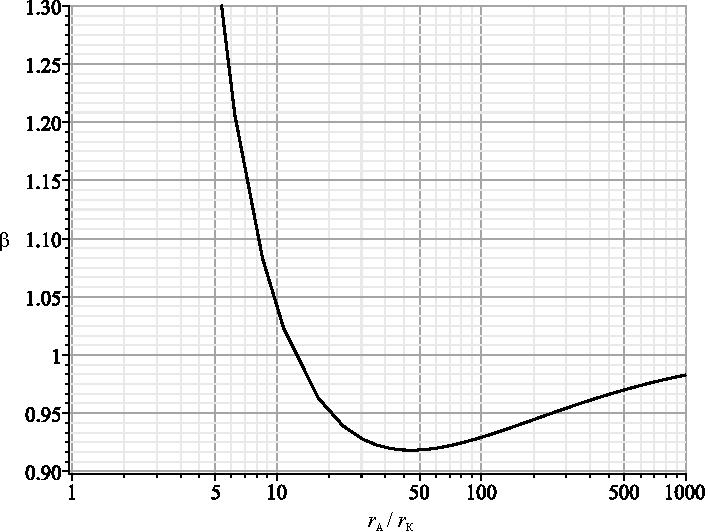
\includegraphics[scale=0.9]{beta.pdf}\par
    \caption{Зависимость поправочного коэффициента $\beta$ от отношения радиусов
        электродов}
    \figmark{beta}
\end{figure}


\experiment 

Исследования проводятся на диоде с косвенным накалом (ток пропускается через 
расположенную вблизи катода \emph{нить накала}). Радиус его 
катода~$r_{К}$, анода~$r_{А}$, а также длина его активной области~$l$ 
указаны на установке. Отметим, что длина
активной области диода (участка катода, покрытого оксидным слоем, обеспечивающим
термоэмиссию электронов) обычно существенно меньше полной
высоты анода (примерно в два раза). Благодаря этому рабочая часть катода достаточно 
удалена от его торцов, и следовательно,
электрическое поле в активной части диода с хорошей точностью можно считать радиальным.

Схема экспериментальной установки изображена на рис.~\figref{Scheme}. Для
питания цепи накала и анода используются два регулируемых источника напряжения. 
Ток накала $I_{н}$ измеряется амперметром, включённым последовательно с
балластным сопротивлением $R$. Анодное напряжение~$U$ измеряется вольтметром, 
а анодный ток $I$~--- миллиамперметром.
В~работе предлагается измерять анодные токи и напряжения в широком диапазоне 
значений (перекрывающем примерно три порядка величины), 
поэтому вольтметр и миллиамперметр должны быть оснащены устройствами 
ручного или автоматического переключения диапазонов измерения.

\begin{figure}[h!]
    \centering
    \pic{9cm}{Chapter_3/3_2_2}
    \caption{Схема экспериментальной установки}
    \figmark{Scheme}
\end{figure}

\labtask

В~работе предлагается исследовать вольт-амперные характеристики диода при
различных токах накала и по результатам
измерений определить удельный заряд электрона.

\begin{lab:task}
    
\item Настройте измерительные приборы согласно прилагаемой к установке
инструкции.

\item Перед включением питания установите ручки регулировки источников
в минимальное положение.

\item Установите минимальный ток накала диода~$I_\text{н}$, 
и минимальное значение анодного напряжения~$V_{A}$, 
указанные в инструкции. Дайте лампе прогреться в течение 5--10 минут.

\item Проведите подробные измерения вольт-амперных характеристик диода 
$I(U)$ во всём допустимом диапазоне изменения напряжений  (см. инструкцию
к установке). 

Всего должно быть измерено не менее 25--30 точек, 
не менее чем по 8--10 на каждый диапазон изменения напряжений. 
Как правило, рекомендуется провести и измерения в диапазоне от 0,5 до 50~В, 
при этом для малых напряжений (до 5~В) измерения рекомендуется производить 
с шагом 0,5~В, для средних (до 15~В)~--- с шагом 1~В и 
для более высоких~--- с шагом 5~В.

\item Повторите измерения вольт-амперных характеристик 
еще при 2--3 рекомендованных значениях токах накала.

\tasksection{Обработка результатов}

\item По результатам проведенных измерений постройте 
вольт-амперные характеристики диода 
в двойном логарифмическом масштабе
$\log I (\log U)$
для каждого тока накала. По графикам определите участки, на которых
выполняется <<закон 3/2>>.

\item Используя данные, соответствующие участкам применимости
<<закона 3/2>>, постройте для каждого тока накала вольт-амперные 
характеристики в координатах $I(U^{3/2})$. 
Убедитесь в том, что зависимость имеет линейный характер. 

\item Найдите наклоны прямолинейных участков зависимости
$I(U^{3/2})$. Используя формулы \eqref{UI_inf}, \eqref{3.2.8}, 
определите удельный заряд электрона~$e/m$.

\item Оцените погрешность результата и сравните его с табличным.

\end{lab:task}


\begin{lab:questions}
    
    \item Каковы условия применимости <<закона 3/2>> для вакуумного диода?
    Почему закон неприменим при малых и больших напряжениях?
    
    \item Изобразите качественно зависимость тока диода от напряжения
    во всём диапазоне положительных напряжений $U_{А}>0$ на аноде.
    
	\item Нарисуйте качественные графики распределения потенциала $\varphi(r)$ 
    между катодом и анодом: а)~в режиме объёмного заряда;
б)~в режиме насыщения тока диода. Объясните эти зависимости.

    \item Как выглядит вольт-амперная характеристика диода при отрицательных
    напряжениях на аноде, $U_{А}<0$?

	\item Как влияет ток накала катода на ток диода при неизменном напряжении
на аноде? Приводит ли это к погрешности измерения~$e/m$?

    \item Получите уравнение \eqref{3.2.1} из интегральной формы теоремы Гаусса
    для электрического поля.
    
    \item Оцените, при каком токе через диод нельзя пренебрегать
    действием магнитного поля этого тока на движение электронов.

\end{lab:questions}

\begin{lab:literature}
	\item \SivuhinIII~--- \S\S100--102.
	\item \Kalashnikov~--- \S157.
\end{lab:literature}


\newpage
\lab{Опыт Милликена.}

\aim{измерение элементарного заряда методом масляных капель.}

\equip{плоский конденсатор в защитном кожухе, осветитель, измерительный микроскоп, электростатический вольтметр,
электронный секундомер, переключатель напряжения, пульверизатор с маслом.}


Идея опыта очень проста. Если элементарный заряд действительно существует, то заряд $q$ любого тела может принимать
только дискретную последовательность значений:
\begin{equation}
	q=0,\,\pm e,\,\pm 2e,\,\pm 3e,\,\ldots\pm ne,\,\ldots,
	\eqmark{3.3.1}
\end{equation}
где $e$~--- элементарный заряд. В предлагаемом опыте измеряется заряд небольших капелек масла, несущих всего несколько элементарных зарядов. Сравнивая между собой заряды капель, можно убедиться, что все они по модулю кратны одному и тому же числу, которое равно, очевидно, элементарному заряду.

Для измерения заряда капель будем исследовать их движение в вертикальном электрическом поле.

Движение заряженной капли в электрическом поле зависит как от электрических сил, так и от массы капли. Масса капли может быть определена по скорости её падения в отсутствие поля.

Рассмотрим свободное падение капли. Уравнение её движения при падении имеет вид
\begin{equation}
	m\frac{dv}{dt}=mg-F_\text{тр},
	\eqmark{3.3.2}
\end{equation}
где $m$~--- масса капли, $v$ --- её скорость, $g$~--- ускорение свободного падения, а $F_\text{тр}$~--- сила вязкого трения капли в воздухе, которая для сферической капли определяется формулой Стокса:
\begin{equation}
	F_\text{тр}=6\pi\eta rv=kv.
	\eqmark{3.3.3}
\end{equation}

Здесь $r$~--- радиус капли, $\eta$~--- коэффициент вязкости воздуха, $k=6\pi\eta r$. Подставляя \eqref{3.3.3} в \eqref{3.3.2}, получим
\begin{equation}
	m\frac{dv}{dt}=mg -kv.
	\eqmark{3.3.4}
\end{equation}

Можно убедиться, что при нулевой начальной скорости решение этого уравнения имеет вид
\begin{equation}
	v=\frac{mg }{k}\left(1-e^{-kt/m}\right).
	\eqmark{3.3.5}
\end{equation}

Установившееся значение скорости равно
\begin{equation}
	v_\text{уст}=\frac{mg }{k}=\frac{\frac 43 \pi\rho r^3g }{6\pi\eta r}=\frac29\frac{\rho}{\eta}g r^2,
	\eqmark{3.3.6}
\end{equation}
где $\rho$~--- плотность масла. Заметим, что \eqref{3.3.6} может быть немедленно получено из \eqref{3.3.4}, если положить $dv/dt=0$.

Как следует из \eqref{3.3.5}, установление скорости происходит с постоянной времени
\begin{equation}
	\tau=\frac{m}{k}=\frac 29 \frac{\rho}{\eta}r^2.
	\eqmark{3.3.7}
\end{equation}
Время установления скорости, таким образом, быстро падает с уменьшением радиуса капли $r$. Для мелких капель оно столь мало, что движение капли всегда можно считать равномерным. Выражение \eqref{3.3.6} в этом случае позволяет определить радиус капли, зная скорость её падения. Обозначая через $h$ путь, пройденный каплей за время $t_0$, найдём
\begin{equation}
	r=\sqrt{\frac{9\eta h}{2\rho g t_0}}.
	\eqmark{3.3.8}
\end{equation}

Рассмотрим теперь движение капли при наличии электрического поля плоского конденсатора, пластины которого расположены горизонтально. Напряжённость поля $E$ в конденсаторе равна
\begin{equation}
	E=\frac{V}{l},
	\eqmark{3.3.9}
\end{equation}
где $l$~--- расстояние между пластинами, а $V$~--- разность потенциалов между ними.

Нас будет интересовать случай, когда под действием электрического поля капля поднимается. Уравнение движения при этом примет вид
\begin{equation}
	m\frac{dv}{dt}=\frac{qV}{l}-mg -kv,
	\eqmark{3.3.10}
\end{equation}
где $q$~--- заряд капли. Появление в правой части постоянного слагаемого не изменяет постоянной времени $\tau$. Для
определения установившейся скорости мы можем снова положить левую часть \eqref{3.3.10} равной нулю.

Измерим время $t$ подъёма капли на начальную высоту. Используя равенства \eqref{3.3.4}, \eqref{3.3.8} и \eqref{3.3.10}, найдём, что заряд капли равен
\begin{equation}
	q=9\pi\sqrt{\frac{2\eta^3 h^3}{g \rho}}\cdot\frac{l(t_0+t)}{Vt_0^{3/2} t}.
	\eqmark{3.3.11}
\end{equation}

Вывод формулы \eqref{3.3.11} предоставляем читателю.

\experiment Схема установки представлена на рис.~\figref{fig3.3.1}. Масло разбрызгивается пульверизатором. Капли масла попадают в конденсатор $C$ через небольшое отверстие в верхней пластине. При этом часть из них вследствие трения о воздух приобретает случайный по абсолютной величине и знаку электрический заряд.

Напряжение на пластины подаётся с регулируемого выпрямителя и измеряется вольтметром $V$. Ключ $K$ позволяет менять направление поля в конденсаторе, чтобы можно было работать  как с отрицательно, так и с положительно заряженными каплями. При размыкании ключа $K$ конденсатор разряжается через дополнительное сопротивление $R\approx 10$~МОм.
\begin{figure}[h!]
	\pic{0.9\textwidth}{3_3_1}
	\caption{Схема экспериментальной установки для измерения заряда электрона}
	\figmark{fig3.3.1}
\end{figure}
Время отсчитывается по электронному секундомеру.

Естественно, что слабые электрические силы, действующие на каплю, несущую всего один или несколько электронных зарядов, способны существенно изменить её движение только в том случае, если сама она очень мала. Опыт производится поэтому с мелкими каплями, наблюдение за которыми возможно только с помощью микроскопа.

В фокальной плоскости окуляра измерительного микроскопа $M$ виден ряд горизонтальных линий, расстояние между которыми было предварительно определено с помощью объектного микрометра. Для облегчения процесса измерений микроскоп может снабжаться камерой с выводом изображения на дисплей ПК. Наблюдая за перемещением капли между линиями, нетрудно определить путь, пройденный каплей. Время $t_0$ свободного падения капли от одной выбранной линии до другой и время $t$ её обратного подъёма, происходящего под действием сил электрического поля, измеряется электронным секундомером.

Из постановки опыта очевидно, что дискретность заряда может быть обнаружена лишь в том случае, если ошибка $\delta q$ в измерении заряда капли существенно меньше абсолютной величины заряда электрона $e$. Допустимая относительная ошибка опыта $\delta q/q$ должна быть поэтому много меньше $e/q=1/n$, где $n$~--- заряд капли, выраженный в числе зарядов электрона. Этому условию тем легче удовлетворить, чем меньше число $n$. В нашем случае трудно определить $q$ с точностью лучше 5\%. Заряд капли должен поэтому быть существенно меньше 20 зарядов электрона~--- лучше всего, если он не превосходит пяти электронных зарядов.

Из всех величин, входящих в формулу \eqref{3.3.11}, на опыте измеряются только $t_0$, $t$, и $V$. От точности определения этих величин зависит в основном ошибка измерения $q$. Из формулы \eqref{3.3.11} можно найти
\begin{equation}
	\frac{\sigma_q}{q}=\sqrt{\frac{\sigma^2_V}{V^2}+\frac{\sigma^2_t t_0^2}{t^2(t_0+t)^2}+
	\frac{\sigma^2_{t_0}}{4t^2_0}\left(\frac{3t+t_0} {t+t_0}\right)^2}.
	\eqmark{3.3.12}
\end{equation}

При $t\approx t_0$ эта формула приобретает вид
\begin{equation}
	\frac{\sigma_q}{q}=\sqrt{\frac{\sigma^2_V}{V^2}+ \frac{\sigma^2_t}{4t^2_0}+ \frac{\sigma^2_{t_0}}{t^2_0}}.
	\eqmark{3.3.13}
\end{equation}

В условиях нашей работы наибольшее влияние на точность эксперимента оказывают два последних стоящих под корнем члена. Ошибка измерения времени $t_0$ и $t$ при визуальном наблюдении капель не может быть сделана меньше 0,1 -- 0,2 секунды. Погрешность в измерении $q$ будет поэтому тем меньше, чем большие значения принимают $t_0$ и $t$. Для увеличения $t_0$ и $t$ можно было бы увеличить расстояние, проходимое каплями, но это сильно усложнило бы экспериментальную установку. Удобнее идти в другом направлении~--- работать с медленно движущимися каплями, т.е. с каплями малого веса. Время падения $t_0$ таких капель достаточно велико. Чтобы время подъёма $t$ было также достаточно большим, нужно использовать не очень большие разности потенциалов $V$.

Заметим, что выбор слишком маленьких капель приводит к снижению точности измерений. Броуновское движение малых капель оказывает существенное влияние на их движение и способно заметно исказить картину их падения и подъёма. Маленькие капли могут испаряться, так что их размеры во время наблюдения могут уменьшаться. При малых скоростях движения делаются особенно опасными конвекционные потоки воздуха, которые возникают при неоднородном нагреве установки (происходящем, например, от осветителя камеры). Практически в наших условиях удобно выбирать $t_0\approx t\approx 10$ -- 30 секунд.

Для капель очень малого размера формула Стокса не вполне применима. Использование формулы Стокса без поправок, впрочем, в наших условиях приводит к искажению значений $q$ и $e$ не более чем на 10\% и почти не мешает обнаружению дискретности электрического заряда. Мы рекомендуем поэтому не вводить в формулу никаких поправок.

\begin{lab:task}

В работе предлагается по измерениям времени свободного падения заряженных капель и времени их подъёма в электрическом поле определить заряд электрона.

\begin{enumerate}

\item{Перед началом работы оцените с помощью формулы \eqref{3.3.11} величину напряжения $V$, которое нужно для подъёма капель, несущих от 1 до 5 зарядов электрона на высоту $h=1$~мм, задав $t_0\approx t=20$~с. Если для подъёма капель потребуются меньшие напряжения, то соответствующие капли слишком сильно заряжены и для эксперимента непригодны.

При вычислениях потребуются значения некоторых величин: расстояние между пластинами $l=0,725$~см; плотность масла
$\rho=0,898$~г/см$^3$; коэффициент внутреннего трения воздуха $\eta=1,83\cdot 10^{-4}$~Пуаз~(СГС) или $1,83\cdot 10^{-5}$~Па$\cdot$с (СИ).}

\item{Включите осветитель. При этом падающий в камеру свет направлен под углом к оси микроскопа и в объектив не попадает. Поле зрения микроскопа остаётся поэтому тёмным. Капли масла рассеивают свет и кажутся светящимися точками на темном фоне.

Не включая электрическое поле \important{слегка} надавите на грушу пульверизатора  и наблюдайте за движением облачка масляных капель в поле зрения микроскопа (изображение перевёрнуто).}

\item{Настройте окуляр микроскопа на резкое изображение делений окулярной шкалы. Затем сфокусируйте объектив на появившиеся в рабочем пространстве капли.}

\item{Наблюдая за движением капель, следует выбирать капли, время падения которых на $h=1$~мм лежит в пределах
10 -- 30 секунд, и научиться отличать их от более крупных, непригодных для работы. Цена деления окулярной шкалы указана на установке.

В случае отсутствия в составе установки ПК с камерой регулировкой и коммутацией напряжения занята одна рука наблюдателя. Вторая рука управляет секундомером. Запись результатов измерений ($t_0$, $t$ и $V$) ведёт второй экспериментатор. Наблюдатель быстро устаёт, поэтому рекомендуется периодически меняться местами. В случае наличия ПК указанные трудности отсутствуют, и работа может быть выполнена одним экспериментатором.

Для уменьшения ошибок в определении $t_0$ и $t$ нужно для пуска и остановки секундомера использовать один и тот же признак~--- всегда нажимать головку секундомера либо в тот момент, когда капля скрывается за линией шкалы, либо, наоборот, когда она появляется из-за линии. Рекомендуется следить за каплей, не отрываясь от окуляра микроскопа, так как в противном случае легко её потерять из виду и весь эксперимент придётся повторить.}

\item{В начале опыта следует позволить капелькам свободно падать \mbox{5 -- 10}~секунд при выключенном электрическом поле для того, чтобы наиболее крупные капли успели упасть на нижнюю пластину.

Из оставшихся в поле зрения капель выберите одну и произведите с ней серию измерений, наблюдая её падение под действием силы тяжести и подъём под действием электрического поля. Серия должна состоять из 5 -- 10 измерений $t_0$ и такого же числа измерений $t$ для одной капли.}

\item{Необходимо проделать не менее 15 таких серий измерений (для 15~различных капель), каждый раз регистрируя величину $V$. При этом нужно иметь в виду, что заряд капли может измениться во время наблюдений; в последнем случае для одной капли получится несколько значений $q$.

Изменение заряда капли может произойти при её подъёме в электрическом поле. Вычисленное с помощью \eqref{3.3.11} значение заряда будет в этом случае соответствовать некоторому среднему из величины заряда капли в начале и в конце опыта. Соответствующий результат непригоден для обработки и только запутывает опыт. Нужно поэтому стараться вовремя отбросить все случаи, когда перезарядка капли произошла во время её подъёма. Это можно сделать, внимательно наблюдая за движением капли и отбрасывая опыты, в которых капля изменила скорость подъёма во время измерения.}

\item{Для оценки точности измерений <<подвесьте>> одну из капель в электрическом поле. Определите соответствующее напряжение, отключите его  и измерьте время падения капли на расстояние 2 -- 3-х делений шкалы. Поменяв полярность напряжения, верните каплю на прежнее место и снова подвесьте её. Снова запишите напряжение. Повторите  процедуру  для одной капли несколько раз  и на месте оцените из этого опыта заряд капли по формуле \eqref{3.3.11}, полагая время подъёма $t=\infty$. По разбросу результатов ($\Delta V$ и  $\Delta t$) оцените точность измерения заряда этой капли.}

\end{enumerate}

\tasksection{Обработка результатов}

\begin{enumerate}

\item{Для всех исследованных капель рассчитайте значения $q$, отложите их на горизонтальной числовой оси и найдите для них общий наибольший делитель. Этот наибольший делитель, вообще говоря, может оказаться равным $e$, $2e$, $3e$ и т.~д. Однако, чем больше значений $q$ было измерено на опыте, тем меньше вероятность получить в качестве делителя число, отличное от $e$. Найденное значение $e$ приведите в системе единиц СИ и в системе СГС.}

\item{Оцените время релаксации $\tau=v_\text{уст}/g$ и расстояние $s$, которое прошла бы капля за это время с установившейся скоростью:
\begin{equation*}
	s=v_\text{уст}\tau=\frac{1}{g}\left(\frac{h}{t_0}\right)^2.
\end{equation*}}

\end{enumerate}

\end{lab:task}

\begin{lab:questions}

\item{Почему не следует выбирать капли слишком большого и слишком маленького размера?}

\item{Какие напряжения соответствуют оптимальным условиям опыта? Приведите расчёты.}

\item{Нарисуйте график зависимости скорости капли в поле силы тяжести от времени и укажите на нём время и путь релаксации.}

\item{Зная параметры установки, оцените ёмкость конденсатора~$C$ и время его разрядки через сопротивление~$R$ (площадь пластин ${\approx} 20$~см$^2$).}

\item{$^*$ Какие ещё способы измерения заряда электрона вам известны?}

\end{lab:questions}

\begin{lab:literature}

\item{ \emph{Сивухин Д.В.} Общий курс физики. Т.~III. Электричество. --- М.:Физматлит, 2015. Гл.~V, \S~90.}

\item{ \emph{Калашников С.Г.} Электричество.~--- М.: Физматлит, 2003. Гл.~XVII, \S~178.}

\end{lab:literature}
\lab{Эффект Холла в полупроводниках}

\aim{измерение подвижности и концентрации носителей заряда в полупроводниках.}

\equip{электромагнит с источником питания, амперметр, миллиамперметр, милливеберметр, реостат, цифровой вольтметр,
источник питания (1,5~В), образцы легированного германия.}

Элементарная теория свободных носителей заряда в~металлах и полупроводниках изложена во введении к разделу.

{\bf Экспериме
нтальная установка.} Электрическая схема установки для измерения ЭДС~Холла представлена на рис.~\ref{fig3.4.1}.

В~зазоре электромагнита (рис.~\ref{fig3.4.1}а) создаётся постоянное магнитное поле, величину которого можно менять с~помощью регулятора~$R_1$ источника питания электромагнита. Ток питания электромагнита измеряется амперметром~А$_1$. Разъём~К$_1$ позволяет менять направление тока в~обмотках электромагнита.

Градуировка магнита проводится при помощи милливеберметра. Описание милливеберметра и правила работы с ним приведены на с.~\pageref{MWB}.

\begin{figure}
%\fcpic[0.9]{3_4_1}
\caption{Схема установки для исследования эффекта Холла в~полупроводниках}
\label{fig3.4.1}
\end{figure}

Образец из легированного германия, смонтированный в~специальном держателе (рис. \ref{fig3.4.1}б), подключается к~источнику питания ($\simeq 1,5$~В). При замыкании ключа~К$_2$ вдоль длинной стороны образца течёт ток, величина которого регулируется реостатом~$R_2$ и измеряется миллиамперметром~А$_2$.

В образце с током, помещённом в зазор электромагнита, между контактами 3 и 4 возникает разность потенциалов~$U_{34}$, которая измеряется с~помощью цифрового вольтметра.

Иногда контакты 3 и 4 вследствие неточности подпайки не лежат на одной эквипотенциали, и тогда напряжение между ними связано не только с~эффектом Холла, но и с~омическим падением напряжения, вызванным протеканием основного тока  через образец. Измеряемая разность потенциалов при одном направлении магнитного поля равна сумме ЭДС~Холла и омического падения напряжения, а при другом~--- их разности. В~этом случае ЭДС ~Холла~$\epsilon_x$ может быть определена как половина алгебраической разности показаний вольтметра, полученных для двух противоположных направлений магнитного поля в~зазоре. Знак измеряемого напряжения высвечивается на цифровом табло вольтметра.

Можно исключить влияние омического падения напряжения иначе, если при каждом токе через образец измерять напряжение
между точками 3 и 4 в~отсутствие магнитного поля. При фиксированном токе через образец это дополнительное к~ЭДС~Холла напряжение~$U_0$ остаётся неизменным. От него следует (с~учётом знака) отсчитывать величину ЭДС~Холла:
\begin{equation}
\epsilon_x=U_{34}\pm U_0.
\label{fig3.4.1}
\end{equation}
При таком способе измерения нет необходимости проводить повторные измерения с~противоположным направлением магнитного поля.

По знаку $\epsilon_x$ можно определить характер проводимости~--- электронный или дырочный. Для этого необходимо знать
направление тока в~образце и направление магнитного поля.

Измерив ток~$I$ в об
разце и напряжение~$U_{35}$ между контактами~3 и 5 в~отсутствие магнитного поля, можно, зная
параметры образца, рассчитать проводимость материала образца по формуле
\begin{equation}
\sigma=\frac{I\, L_{35}}{U_{35}\,a\,l},
\label{eq3.4.2}
\end{equation}
где $L_{35}$~--- расстояние между контактами 3 и 5, $a$~--- толщина образца, $l$~--- его ширина.

{\Large \bf ЗАДАНИЕ}

В работе предлагается исследовать зависимость ЭДС~Холла от величины магнитного поля при различных токах через образец для определения константы Холла; определить знак носителей заряда и проводимость материала образца.

\begin{enumerate}
\item{ Подготовьте приборы к работе.}

\item{ Проверьте работу цепи питания образца. Ток через образец не должен превышать 1~мА.}

\item{ Проверьте работу цепи магнита. Определите диапазон изменения тока через магнит.}

\item{ Прокалибруйте электромагнит~--- определите связь между индукцией~$B$ магнитного поля в зазоре электромагнита и током $I_M$ через обмотки магнита. Для этого с помощью милливеберметра снимите зависимость магнитного потока $\Phi$, пронизывающего пробную катушку, находящуюся в~зазоре, от тока~$I_M$ ($\Phi=BSN$). Значение $SN$ (произведение площади сечения контура катушки на число витков в ней) указано на держателе катушки.}

\item{ Проведите измерение ЭДС Холла. Для этого вставьте образец в~зазор выключенного электромагнита и определите напряжение~$U_0$ между холловскими контактами 3 и 4 при минимальном токе через образец ($\simeq 0,2$~мА). Это напряжение~$U_0$ вызвано несовершенством контактов~3, 4 и при фиксированном токе через образец остаётся неизменным. Значение~$U_0$ с~учётом знака следует принять за нулевое.

Включите электромагнит и снимите зависимость напряжения~$U_{34}$ от тока~$I_M$ через обмотки магнита при фиксированном токе через образец.

Проведите измерения $U_{34}=f(I_{M})$ при постоянном токе через образец для 6--8 его значений в~интервале 0,2--1~мА. При каждом новом значении тока через образец величина~$U_0$ будет иметь своё значение.

При максимальном токе через образец ($\simeq 1$~мА) проведите измерения $U=f(I_{M})$ при другом направлении магнитного поля.
}
\item{ Определите знак носителей в образце. Для этого необходимо знать направление тока через образец, направление магнитного поля и знак ЭДС Холла.

Направление тока в образце показано знаками~<<+>> и <<$-$>> на рис. \ref{fig3.4.1}. Направление тока в~обмотках электромагнита при установке разъёма~K$_1$ в~положение~I показано стрелкой на торце магнита.

Зарисуйте в тетради образец. Укажите на рисунке направления тока, магнитного поля и отклонение носителей. По знаку
($\pm$) на клеммах цифрового вольтметра определите характер проводимости.
}
\item{Для определение удельной проводимости удалите держатель с~образцом из зазора. Подключите к~клеммам~<<$H_{x}$>> и <<$L_{x}$>> вольтметра потенциальные концы~3 и 5. Измерьте падение напряжения между ними при токе через образец 1~мА.}

\item{ Запишите характеристики приборов и параметры образца $L_{35}$, $a$, $l$, указанные на держателе.}
\end{enumerate}

{\rm Обработка результатов}
\begin{enumerate}

\item {Постройте график зависимости $B=f(I_{M})$.}

\item{ Рассчитайте ЭДС~Холла по формуле~(\ref{eq3.4.1}) и постройте на одном листе семейство характеристик $\epsilon_x=f(B)$ при разных значениях тока~$I$ через образец. Определите угловые коэффициенты~$k(I)=\Delta{\epsilon_x}/\Delta B$ полученных прямых.

Постройте график $k=f(I)$. Рассчитайте угловой коэффициент прямой и по формуле~(TO ADD REF) Приложения определите величину постоянной Холла~$R_{X}$. Рассчитайте концентрацию~$n$ носителей тока в~образце по формуле ([TO ADD REF]).

Оцените погрешность результата и сравните результат с~табличным.}


\item{ Рассчитайте удельную проводимость~$\sigma$ материала образца по формуле~(\ref{eq3.4.2}).

Используя найденные значения концентрации~$n$ и проводимости~$\sigma$, с~помощью формулы~([TO ADD REF]) вычислите подвижность~$b$ носителей тока в~общепринятых для этой величины внесистемных единицах: размерность напряжённости электрического поля $[E]=[U/L]=$~B/см, размерность скорости $[v]=$~см/с, поэтому размерность
подвижности~$[b]=$см$^2$/(В$\cdot$с).

Оцените погрешности и сравните результаты с~табличными.}
\end{enumerate}

{\small

{\bf \Large Контрольные вопросы}
\begin{enumerate}



\item{ Какие вещества называют диэлектриками, проводниками, полупроводниками? Чем объясняется различие их электрических свойств? Как зависит от температуры проводимость металлов и полупроводников?}

\item{ Дайте определение константы Холла. Как зависит константа Холла от температуры у металлов и полупроводников?}

\item{ Зависит ли результат измерения константы Холла от геометрии образца?}

\item{ Как устроен милливеберметр? Зависят ли его показания от сопротивления измерительной катушки? Каким должно быть это сопротивление по сравнению с сопротивлением катушки прибора: большим или маленьким?}

\item{ Получите выражение константы Холла для материалов с~двумя типами носителей. При выводе используйте условие равенства нулю поперечного тока.}

\end{enumerate}

{\bf \Large Список литераратуры}

\begin{enumerate}


\item{ \emph{Сивухин Д.В.} Общий курс физики. Т.~III. Электричество~--- М.: Наука, 1983. \S\S~98, 100.}

\item{ \emph{Парселл Э.} Электричество и магнетизм.~--- М.: Наука, 1983. Гл.~4, \S\S~4--6; Гл.~6, \S~9 (Берклеевский курс физики. Т.~II).
    }

\end{enumerate}
}



{\large \bf 3.3.5 Эффект Холла в металлах}

{\bf Цель работы:}{измерение подвижности и концентрации носителей заряда в металлах.}

{\bf В работе используются:}{электромагнит с источником питания, источник постоянного тока, микровольтметр Ф116/1, амперметры, милливеберметр,
образцы из меди, серебра и цинка.}

Элементарная теория свободных носителей заряда в~металлах и полупроводниках изложена во введении к разделу.

{\bf Экспериментальная установка.} Электрическая схема установки для измерения ЭДС~Холла представлена на рис.~\ref{fig3.5.1}.

\begin{figure}
%\fcpic[0.9]{3_5_1}
\caption{Схема установки для исследования эффекта Холла в~металлах}
\label{fig3.5.1}
\end{figure}

В зазоре электромагнита (рис \ref{fig3.5.1}а) создаётся постоянное магнитное поле, величину которого можно менять с~помощью источника питания электромагнита. Разъём~К$_1$ позволяет менять направление тока в~обмотках электромагнита. Ток питания электромагнита измеряется амперметром~А$_1$.

Градуировка магнита проводится с~помощью милливеберметра. Описание милливеберметра и правила работы с ним приведены на с.~\pageref{MWB}.

Металлические образцы в форме тонких пластинок, смонтированные в~специальных держателях, подключаются к~блоку питания через разъём (рис \ref{fig3.5.1}б). Ток через образец регулируется реостатом~$R_2$ и измеряется амперметром~А$_2$.

Для измерений ЭДС Холла используется микровольтметр Ф116/1, в~котором высокая чувствительность по напряжению сочетается с~малой величиной тока, потребляемого измерительной схемой: минимальный предел измерения напряжения составляет~1,5~мкВ, а потребляемый ток~--- всего~$10^{-8}$~А.

В~образце с~током, помещённом в~зазор электромагнита, между контактами~2 и 4 возникает холловская разность потенциалов, которая измеряется с~помощью микровольтметра, если переключатель К$_3$ подключён к~точке~2 образца. При подключении К$_3$ к~точке~3 микровольтметр измеряет омическое падение напряжения~$U_{34}$, вызванное основным током через образец. При нейтральном положении ключа входная цепь микровольтметра разомкнута.

Ключ К$_2$ позволяет менять полярность напряжения, поступающего на вход микровольтметра.

Иногда контакты~2 и 4 вследствие неточности подпайки не лежат на одной эквипотенциали, и тогда напряжение между ними связано не только с~эффектом Холла, но и с~омическим падением напряжения, вызванным протеканием основного тока через образец. Измеряемая разность потенциалов при одном направлении магнитного поля равна сумме ЭДС~Холла и омического падения напряжения, а при другом~--- их разности. В~этом случае ЭДС Холла $\epsilon_x$ может быть определена как половина
алгебраической разности показаний вольтметра, полученных для двух противоположных направлений магнитного поля в~зазоре.


Можно исключить влияние омического падения напряжения иначе, если при каждом токе через образец измерять
напряжение~$U_0$ между точками~2 и 4 в~отсутствие магнитного поля. При фиксированном токе через образец это
дополнительное к ЭДС Холла напряжение остаётся неизменным. От него следует (с~учётом знака) отсчитывать величину
ЭДС Холла:
\begin{equation}
\epsilon_x=U_{24}\pm U_0.
\label{eq3.5.1}
\end{equation}
При таком способе измерения нет необходимости проводить повторные измерения с~противоположным направлением магнитного поля.

По знаку $\epsilon_x$ можно определить характер проводимости~--- электронный или дырочный. Для этого необходимо знать
направление тока в~образце и направление магнитного поля.

Измерив ток $I$ в образце и напряжение~$U_{34}$ между контактами~3 и 4 в~отсутствие магнитного поля, можно, зная
параметры образца, рассчитать проводимость материала образца по очевидной формуле:

\begin{equation}
\sigma=\frac{I\, L_{34}}{U_{34}\, al},
\end{equation}

где $L_{34}$~--- расстояние между контактами~3 и 4, $a$~--- толщина образца, $l$~--- его ширина.

{\Large \bf ЗАДАНИЕ}

В работе предлагается исследовать зависимость ЭДС~Холла от величины магнитного поля при различных токах через образец для определения константы Холла; определить знак носителей заряда и проводимость различных металлических образцов.

\begin{enumerate}

\item{Подготовьте приборы к работе.}

\item{ Проверьте работу цепи питания образца. Для этого подключите к разъёму блока управления один из образцов~--- медный или серебряный. Убедитесь, что ток через образец можно изменять от 0,5 до 1,2~А.}
\item{ Проверьте работу цепи магнита. Установите разъём К$_1$ в положение I и определите диапазон изменения тока через электромагнит.}
\item{ Прокалибруйте электромагнит. Для этого вставьте в зазор электромагнита пробную катушку милливеберметра и исследуйте зависимость магнитного потока~$\Phi$, пронизывающего пробную катушку, от тока $I_M$ через обмотки магнита ($\Phi=BSN$).
Значение $SN$ (площадь сечения пробной катушки на число витков в ней) указано на держателе катушки.

Проведите измерения магнитного потока для 6--8 значений тока через электромагнит.}

\item{ Проведите измерение ЭДС Холла. Для этого вставьте образец в~зазор выключенного электромагнита и определите напряжение~$U_0$ между холловскими контактами 2 и 4 при минимальном токе через образец ($\simeq 0,5$~А). Это напряжение~$U_0$ вызвано несовершенством контактов~2, 4 и при фиксированном токе через образец остаётся неизменным. Значение~$U_0$ с~учётом знака следует принять за нулевое.

Включите электромагнит и снимите зависимость напряжения~$U_{24}$ от тока~$I_M$ через обмотки магнита при фиксированном токе через образец. Измерения следует проводить при {\bf медленном} увеличении магнитного поля. Резкие изменения магнитного поля наводят ЭДС индукции в~подводящих проводах и вызывают большие отклонения стрелки микровольтметра.

Повторите измерения $U=f(I_{M})$ при постоянном токе через образец для 5--6 его значений в~интервале $0,5-1,2$~А. При каждом новом значении тока через образец величина~$U_0$ будет иметь своё значение.

При максимальном токе через образец проведите измерения $U=f(I_{M})$ при другом направлении магнитного поля.

Для образца из цинка снимите зависимость $U=f(I_{M})$ при одном значении тока через образец ($I\simeq 1$~А).}

\item{Определите знак носителей в образце. Для этого необходимо знать направление тока через образец, направление магнитного поля и знак ЭДС Холла. Направление тока в образце показано знаками~<<+>> и <<$-$>> на рис. \ref{fig3.4.1}. Направление тока в~обмотках электромагнита при установке разъёма~K$_1$ в~положение~I показано стрелкой на торце магнита.

Напомним, что знак потенциала, соответствующий точкам 2 или 4, можно определить по рис. \ref{fig3.4.1}.

Зарисуйте в тетради образец. Укажите на рисунке направление тока, магнитного поля (положение разъёма~K$_1$) и знак
потенциала, соответствующий клемме~4 (положение ключа~K$_2$ при отклонении стрелки вольтметра вправо).

Определите знак носителей заряда для каждого из двух образцов.
}
\item{Определите удельную проводимость образца. Для этого удалите держатель с~образцом из зазора. Установите переключатель микровольтметра <<ПРЕДЕЛЫ ИЗМЕРЕНИЯ>> на 750~мкВ. Ключ~K$_3$ поставьте в~положение~$U_{34}$. При токе через образец~$\sim 1$~А измерьте падение напряжения между контактами 3 и 4 для каждого из двух образцов.}

\item{ Запишите характеристики приборов и параметры образцов $L_{34}$ $a$, $l$, указанные на держателях.}
\end{enumerate}

{\rm Обработка результатов}
\begin{enumerate}
\item{Рассчитайте индукцию магнитного поля~$B$ для каждого значения тока и постройте график зависимости $B=f(I_{M})$.}

\item{Рассчитайте ЭДС Холла по формуле~(\r1) и постройте на одном листе семейство характеристик $\epsilon_x=f(B)$ при разных значениях тока~$I$ через образец (для меди или серебра). Определите угловые коэффициенты~$k(I)=\Delta\epsilon/\Delta B$ полученных прямых.}

\item{ Постройте график $k=f(I)$. Рассчитайте угловой коэффициент прямой и по формуле~([TO ADD REF]) определите величину постоянной Холла $R_x$.

Для цинка изобразите на графике зависимость $\epsilon_x=f(B)$ и по наклону прямой рассчитайте постоянную Холла.

Для обоих образцов рассчитайте концентрацию~$n$ носителей тока по формуле ([TO ADD REF]).

Оцените погрешности и сравните результаты с~табличными.}

\item{ Рассчитайте удельную проводимость~$\sigma$ материала образцов по формуле~(\ref{eq3.5.1}).

Используя найденные значения концентрации~$n$ и проводимости~$\sigma$, с~помощью формулы~([TO ADD REF]) рассчитайте подвижность~$b$ носителей тока в~общепринятых для этой величины внесистемных единицах: размерность напряжённости электрического поля~$[E]=[U/L]=В/см$, размерность скорости~$[v]=см/с$, поэтому размерность подвижности $[b]=$см$^2$/(В$\cdot$с).

Оцените погрешности и сравните результаты с табличными.
}
\end{enumerate}

{\small

{\bf \Large Контрольные вопросы}

\begin{enumerate}

\item{ Какие вещества называют диэлектриками, проводниками, полупроводниками? Чем объясняется различие их электрических свойств? Как зависит от температуры проводимость металлов и полупроводников?}

\item{ Дайте определение константы Холла. Как зависит константа Холла от температуры у~металлов и полупроводников?}

\item{ Зависит ли результат измерения константы Холла от геометрии образца?}

\item{ Как устроен милливеберметр? Зависят ли его показания от сопротивления измерительной катушки? Каким должно быть это сопротивление по сравнению с~сопротивлением рамки прибора: большим или маленьким?}

\end{enumerate}

{\bf \Large Список литераратуры}

\begin{enumerate}


\item{ \emph{Сивухин Д.В.} Общий курс физики. Т.~III. Электричество~--- М.: Наука, 1983. \S\S~98, 100.}

\item{ \emph{Парселл Э.} Электричество и магнетизм.~--- М.: Наука, 1983. Гл.~4, \S\S~4--6; Гл.~6, \S~9 (Берклеевский курс физики. Т.~II).}
\end{enumerate}

}



\lab{Влияние магнитного поля на проводимость полупроводников}

\aim{измерение зависимости сопротивления 
    полупроводниковых образцов различной формы от магнитного поля.}

\equip{электромагнит, милливеберметр или миллитесламетр (на основе датчика
Холла), вольтметр, амперметр, миллиамперметр, реостат, образцы
монокристаллического антимонида индия (InSb) $n$-типа.}

Перед выполнением работы необходимо ознакомиться с основами
элементарной теории движения носителей заряда в~металлах и полупроводниках
(п. \ref{sec:halleffect} Введения к разделу).

В работе изучается зависимость проводимости полупроводников от магнитного поля
в геометрии \emph{диска Корбино}.
По диску, помещенному в перпендикулярное ему магнитное поле, пропускается
ток в радиальном направлении. Магнитное поле искривляет линии 
тока, благодаря чему эффективное сопротивление образца возрастает
(эффект \emph{геометрического магнетосопротивления}). По результатам
измерений зависимости сопротивления от магнитного поля 
могут быть вычислены подвижность и концентрация носителей тока в образце.

\experiment
Схема установки для исследования магнетосопротивления
полупроводников и геометрического резистивного эффекта представлена на
рис.~\figref{Scheme}.

\begin{figure}[h!]
    \centering
    \pic{0.9\textwidth}{Chapter_3/3_6_1}
    \caption{Схема установки для~исследования влияния магнитного~поля
        на~проводимость полупроводников}
    \figmark{Scheme}
\end{figure}

В зазоре электромагнита (рис.~\figref{Scheme}а) создаётся постоянное магнитное
поле, величину которого можно менять с помощью источника питания электромагнита.
Ток электромагнита измеряется амперметром А$_1$ (отдельным или встроенным в источник).
Магнитная индукция в зазоре измеряется при помощи милливеберметра (его описание
и правила работы с ним приведены на с.~\pageref{MWB}) или 
миллитесламетра на основе датчика Холла.

Образец в форме кольца (диск Корбино) или пластинки, смонтированный в
специальном держателе, подключается к источнику постоянного напряжения 5~В. При
замыкании ключа~К$_2$ сквозь образец течёт ток, величина которого измеряется
миллиамперметром~А$_2$ и регулируется реостатом~$R_2$. Балластное сопротивление~$R_0$
ограничивает ток через образец. Измеряемое напряжение подаётся на вход
вольтметра~V.

\labtask


В работе предлагается при постоянном токе через образец исследовать зависимость
напряжения на образце от величины магнитного поля и от ориентации образца в
магнитном поле; по результатам измерений рассчитать подвижность электронов,
удельное сопротивление материала образца и концентрацию электронов.

\begin{lab:task}

\item Подготовьте приборы к работе согласно описанию на установке.

\item Концы от точек~3 и~4 разъёма подсоедините к клеммам вольтметра.
Присоедините диск Корбино через разъём к цепи питания. Определите
диапазон изменения силы тока через образец.

\item Установите ручки регулировки источника питания электромагнита 
в минимальное положение и включите источник. 
Плавно меняя ток магнита, определите диапазон его изменения.

\item Измерьте калибровочную кривую электромагнита~---
зависимость между индукцией~$B$ магнитного поля в его зазоре и 
током~$I_{М}$ через обмотки магнита.
Магнитное поле измеряется милливеберметром или миллитесламетром
(датчиком Холла). Калибровочная кривая должна содержать не менее
15 точек во всём диапазоне изменения токов.

В~случае использования милливеберметра измерьте зависимость 
магнитного потока~$\Phi$, пронизывающего пробную катушку, 
находящуюся в зазоре, от тока~$I_{М}$ ($\Phi=BSN$). 
Значение~$SN$ (произведение площади сечения контура катушки на
число витков в ней) указано на держателе катушки.

\item \label{p1} Вставьте образец в зазор \emph{выключенного} электромагнита 
и измерьте падение напряжения $U_0$ в образце при некотором токе,
рекомендованном в описании ($I_0\sim 25$~мА). 

\item \label{p2} Включите электромагнит и измерьте зависимость напряжения~$U$ 
на образце от тока через обмотки магнита~$I_M$ при фиксированном токе
через образец~$I_0$.

\item Проверьте, что результат измерения не зависит от направления магнитного
поля.

%\item Повторите измерения пп. \ref{p1}, \ref{p2} 
%для 3--4 других значений тока $I_0$ через образец.

\item Вместо диска Корбино подключите к измерительной цепи образец, имеющий
форму пластинки. Поместите образец в зазор выключенного электромагнита и
измерьте падение напряжения~$U_0$ на образце при токе через образец $10$~мА.

\item Включите электромагнит и снимите зависимость напряжения~$U$ на образце от
тока через магнит при постоянном токе $I=10$~мА. При измерениях длинная сторона
образца должна быть направлена поперёк поля, а средняя (ширина) в~одной серии
опытов располагается вдоль, а в другой~--- поперёк поля.

\item Запишите геометрические размеры образцов и характеристики приборов.

\tasksection{Обработка результатов}

\item Постройте калибровочный график зависимости $B(I_{M})$. 
    Используйте эту зависимость для дальнейшего пересчёта (интерполяции)
    значений поля по измеренным токам $I_{М}$.

\item Для всех серий измерений постройте графики, отложив по оси абсцисс
величину~$B^2$, а по оси ординат~--- величину $(U-U_0)/U_0$. Какие выводы
можно сделать на основании построенных зависимостей?

\item По наклону прямолинейного участка графика для диска Корбино рассчитайте
с помощью формулы \chaptereqref{MagnetoSoprot} подвижность носителей.

\item Определите сопротивление диска $R_0$ в отсутствие магнитного поля.
По геометрическим размерам образца рассчитайте удельное сопротивление~$\rho_0$ 
и удельную проводимость $\lambda_0=1/\rho_0$ материала образца.

\item С помощью формулы \chaptereqref{3.26} найдите концентрацию носителей
тока.

\item Оцените погрешности и сравните результаты с табличными.

\end{lab:task}


\begin{lab:questions}

\item Какие вещества называют диэлектриками, проводниками, полупроводниками?
Чем объясняется различие их электрических свойств? Как зависит от температуры
проводимость металлов и полупроводников?

\item В чем причина зависимости сопротивления образца от магнитного
поля в геометрии диска Корбино?

\item Зависит ли эффект магнетосопротивления от геометрии образца? 
В каких случаях эффект магнетосопротивления может проявиться
при протекании тока по плоской пластинке?

\item Как устроен милливеберметр? Зависят ли его показания от сопротивления
измерительной катушки? Каким должно быть это сопротивление по сравнению с
сопротивлением рамки прибора: большим или маленьким?

\item По результатам измерений оцените частоту столкновений,
длину пробега и коэффициент диффузии носителей тока в исследуемом материале.

\item Получите выражение для сопротивления пластинки, изготовленной
из материала с~двумя типами носителей. 
Для простоты можно ограничиться случаем $\mu_e \gg \mu_h$.

\end{lab:questions}


\begin{lab:literature}
\item \SivuhinIII~--- \S\S~98, 100.
\item \textit{Парселл Э.} Электричество и магнетизм.~--- М.: Наука, 1983. Гл.~4,
\S\S~4--6; Гл.~6, \S~9.
\end{lab:literature}


%\newpage
%\begin{labsupplement}[Принцип действия милливеберметра]
\label{MWB}

\term{Милливеберметр} (\term{флюксметр}) служит для измерения постоянного во времени
магнитного потока. Это прибор магнитоэлектрической системы, 
работающий в баллистическом режиме: рамка с током вращается в поле 
постоянного магнита; отклонение рамки пропорционально заряду,
если через неё пропускается короткий импульс тока. 
От обычных гальванометров постоянного тока милливеберметр 
отличается тем, что на его рамку не действуют никакие упругие силы, 
поэтому его подвижная часть находится в безразличном равновесии.

\begin{wrapfigure}{o}{2.5cm}
    \centering
    \pic{2.5cm}{Chapter_3/mwb-01}
    \caption{Рамка в магнитном поле}
    \figmark{Frame in a magnetic field}
\end{wrapfigure}

В цепь рамки прибора включается наружная измерительная (пробная) катушка. 
При изменении магнитного потока, пронизывающего эту катушку, 
в ней возникает ЭДС индукции, и по цепи рамки течёт индукционный ток. 
При этом отклонение рамки, независимо от её начального
положения, пропорционально изменению магнитного потока $\Delta\Phi$ 
и может служить для его измерения.

Рассмотрим детально работу милливеберметра. 
Уравнение моментов для рамки имеет вид
\begin{equation}
    J\ddot{\varphi}=M,
    \eqmark{MWB.1}
\end{equation}
где $J$~--- момент инерции рамки, 
$\varphi$~--- угол её поворота (рис.~\figref{Frame in a magnetic field}),
$M$ --- момент сил Ампера, действующих на рамку.
Последний вычисляется как произведение силы Ампера $F=IlNB_0$, 
действующей на каждую из продольных сторон,
на удвоенное плечо, т.е. на поперечный размер
рамки $a$. Здесь $I$~--- сила тока в рамке, $l$~--- длина продольной
стороны, $N$~--- число витков намотанного на рамку провода, 
$B_0$~--- индукция поля постоянного магнита милливеберметра. 
Поле магнита практически радиально, и его величина не зависит от угла поворота
рамки, что обеспечивает равномерность шкалы прибора. 

Таким образом, вводя обозначение $K=alNB_0$, из \eqref{MWB.1} 
получим
\begin{equation}
    J\ddot{\varphi}=KI.
    \eqmark{MWB.2}
\end{equation}

Рассмотрим теперь уравнение цепи, в которую включена рамка.
Ток~$I$ в рамке генерируется под действием как внешней ЭДС
индукции $\mathcal{E}_{К}$, возникающей в измерительной катушке, так и внутренней
$\mathcal{E}_{Р}$, возникающей в рамке при её вращении в магнитном поле:
\begin{equation}
    RI=\mathcal{E}_{К}+\mathcal{E}_{Р},
    \eqmark{MWB.3}
\end{equation}
где $R$~--- полное сопротивление цепи рамки.

Внешняя ЭДС $\mathcal{E}_{К}$ наводится в измерительной катушке при изменении
проходящего сквозь неё магнитного потока~$\Phi$:
\begin{equation}
    \mathcal{E}_{К}=-\frac{d\Phi}{dt}.
    \eqmark{MWB.4}
\end{equation}

ЭДС в рамке $\mathcal{E}_{Р}$ возникает в её продольных сторонах 
при их движении в поле $B_0$ со скоростью $v=\dot{\varphi}a/2$:
\begin{equation}
    \mathcal{E}_{Р}=-2lNB_0\frac{a}{2}\dot\varphi=-K\dot\varphi.
    \eqmark{MWB.5}
\end{equation}

Подставим \eqref{MWB.3}--\eqref{MWB.5} в \eqref{MWB.2} и получим уравнение 
движения рамки:
\begin{equation}
    \frac{JR}{K^2}\ddot{\varphi}+\dot{\varphi}=-\frac{1}{K}\dot{\Phi}.
    \eqmark{MWB.6}
\end{equation}

Проинтегрируем полученное уравнение по времени. Получим
\begin{equation}
\frac{JR}{K^2} \Delta \dot{\varphi}+
\Delta \varphi = -\frac{\Delta \Phi}{K},
    \eqmark{MWB.7}
\end{equation}
где $\Delta$ обозначает разность между конечным и начальным состояниями.

Покажем, что первое слагаемое \eqref{MWB.7} мало и им можно пренебречь.
В~начальный момент рамка неподвижна
($\dot{\varphi}_1=0$). Пусть в конце измерения поток через 
измерительную катушку постоянен, $\dot{\Phi}=0$. Тогда в уравнении
\eqref{MWB.6} правая часть равна нулю, и его решение есть 
экспоненциально затухающая функция:
\begin{equation*}
\dot{\varphi}=\dot{\varphi}_0\,\exp\left(-\frac{K^2}{JR}t\right).
\end{equation*}
Следовательно, по прошествии времени $\tau=JR/K^2$ рамка практически
остановится: $\dot{\varphi}(t)\to0$ при $t\gg\tau$. Подбирая достаточно малое 
сопротивление цепи~$R$, можно добиться того, чтобы
время торможения рамки~$\tau$ было достаточно малым в условиях опыта.

Таким образом, угол поворота рамки милливеберметра оказывается прямо пропорционален 
изменению магнитного потока через измерительную катушку:
\begin{equation}
\Delta \varphi=-\frac{\Delta \Phi}{K} .
\eqmark{MWB.9}
\end{equation}

Для измерения магнитного потока с помощью милливеберметра можно:

а) вынести измерительную катушку из области измеряемого в область нулевого поля;

б) оставив катушку в поле неподвижной, отключить измеряемое поле.

Разделив поток $\Delta \Phi$ на площадь и число витков измерительной катушки, 
можно определить изменение индукции~$\Delta B$ внешнего магнитного поля,
пронизывающего катушку.
Отметим, что в обоих вариантах поток в конце опыта постоянен, как того
требует сделанное выше предположение.

\end{labsupplement}

%Обратим внимание на структуру формулы \eqref{MWB.8}. Время~$t$, в течение
%которого затухает движение рамки, должно быть небольшим, так как рамка находится
%в~безразличном равновесии и склонна дрейфовать. Самопроизвольное перемещение
%стрелки искажает результаты измерений. Из \eqref{MWB.8} видно, что время
%успокоения прибора падает с уменьшением~$R$, поэтому милливеберметр работает
%правильно лишь при замыкании его рамки на достаточно малое сопротивление.
%Допустимая величина сопротивления измерительной катушки указана на приборе.

%Принципиальная схема милливеберметра изображена на рис.~\figref{Device scheme}.
%Так как прибор не имеет противодействующего механического момента, стрелка его
%после измерения не возвращается к начальному положению. Для установки стрелки на
%нужную отметку служит электромагнитный корректор~--- вторая магнитная система,
%состоящая из постоянного магнита и сердечника с обмоткой. Когда ручка
%переключателя находится в положении <<Корректор>>, обмотка корректора замкнута
%на рамку прибора, в которой в момент поворота ручки корректора (вследствие
%пересечения силовых линий магнита корректора) возникает ток.
%Изменяя направление и угол поворота ручки корректора, можно установить стрелку
%прибора на любом делении шкалы.
%\begin{figure}[h!]
%%    \pic{0.9\textwidth}{mwb-02}
%    \caption{Схема прибора}
%    \figmark{Device scheme}
%\end{figure}
%При положении ручки переключателя на отметке <<Арретир>> рамка прибора замкнута
%накоротко, и подвижная система прибора находится в сильно успокоенном режиме.
%
%В положении <<Измерение>> прибор готов к работе.
%
%\labsection{ПРАВИЛА РАБОТЫ}
%
%\labsection{Общие указания}
%
%\begin{enumerate}
%
%\item{Для измерения магнитного потока подключённая к прибору измерительная
%катушка помещается в магнитное поле перпендикулярно ему.}
%
%\item{Для исключения погрешности от паралакса отсчёт показаний следует проводить
%так, чтобы изображение стрелки в зеркале шкалы совпадало с самой стрелкой.}
%\end{enumerate}
%
%\labsection{Измерение магнитного потока}
%
%\begin{enumerate}
%
%\item{Поставьте переключатель в положение <<Корректор>> и поворотом рукоятки
%корректора установите начальное положение стрелки, удобное для измерений.
%
%Если ручка корректора дошла до упора, а стрелка сместилась недостаточно,
%поверните рукоятку корректора в обратную сторону до упора, а затем снова
%поворачивайте её, пока стрелка не встанет на нужное деление.}
%
%\item{Поставьте переключатель в положение <<Измерение>>. Заметьте начальное
%положение стрелки (вся шкала --- 10 дел. --- 10~mWb).
%
%Измените магнитный поток сквозь катушку до нуля и заметьте новое положение
%стрелки. Разность показаний определяет магнитный поток.
%
%Изменять магнитный поток рекомендуется одним из способов:
%
%а) быстро удаляя пробную катушку из области действия магнитного поля на
%расстояние, где магнитный поток практически равен нулю (рекомендуется);
%
%б) выключая магнитное поле, если катушка закреплена жёстко.
%
%Не рекомендуется переполюсовывать магнит для измерений поля, т.~к. при этом
%часто ломаются переключатели.
%
%Величина $SN$, необходимая для расчёта индукции поля, указана на пробной
%катушке.}
%
%\item{По окончании работы следует заарретировать прибор~--- поставить
%переключатель в положение <<Арретир>>.}
%
%\item{Не реже одного раза в месяц рекомендуется проверять состояние приборов по
%образцовому прибору.}

%Один раз в два года, а также после каждого ремонта, приборы должны проверяться
%в местном отделении Комитета стандартов, мер и измерительных приборов.

%\end{enumerate}



\cleardoublepage
\chapter{Магнитные свойства вещества}

Известно, что вещество может обладать как собственной намагниченностью, так
и изменять свою намагниченность при помещении во внешнее магнитное поле.
Источниками магнитного поля в среде могут служить орбитальное движение электронов
в молекулах и атомах, а также собственное вращение (спин) электронов и ядер.
Не вдаваясь в детальное описание микроскопических свойств среды, можно считать,
что каждый элемент объёма среды может являться элементарным источником
магнитного поля --- \important{магнитным диполем}. Для описания усреднённых
(макроскопических) свойств среды используют
\important{вектор намагниченности} $\vec{M}$, равный
\emph{магнитному моменту единичного объёма вещества} (объёмная плотность магнитного момента).

Среднее значение магнитного поля в некоторой точки среды есть вектор
$\vec{B}$, называемый (по историческим причинам) \important{индукцией поля}.
Помимо этого, принято вводить вспомогательный вектор $\vec{H}$
(\important{напря\-жённость поля}), определяемый из соотношения
\begin{equation}
    \eqmark{fieldB}
    \vec{B} = \mu_0(\vec{H} + \vec{M}).
\end{equation}

В простейшем практически важном случае намагниченность $\vec{M}$ в каждой
точке среды прямо пропорциональна вектору напряжённости магнитного
поля~$\vec{H}$ в этой же точке:
\begin{equation}
    \eqmark{magnetization}
    \vec{M} = \chi\vec{H}.
\end{equation}
Коэффициент $\chi$ называют \important{магнитной восприимчивостью} среды.
Вещества, для которых закон \eqref{magnetization} выполняется
с хорошей точностью, называют \important{парамагнетиками} ($\chi > 0$) и
\important{диамагнетиками} ($\chi < 0$).
В~парамагнетиках элементарные диполи
ориентированы в основном по приложенному полю,
а в диамагнетиках --- против него.

Если закон \eqref{magnetization} применим,
то можно записать
\begin{equation}
    \vec{B} = \mu\mu_0 \vec{H},\qquad \text{где }\mu = 1 + \chi
\end{equation}
--- \important{магнитная проницаемость} вещества%
\footnote{В системе СГС имеют место соотношения
    $\vec{B}=\vec{H}+4\pi\vec{M}=\mu\vec{H}$, $\mu = 1 + 4\pi \chi$.}.

Отметим. что в общем случае зависимость $\vec{M}$ от $\vec{H}$ в среде может
не только быть нелинейной, но и зависеть от ``предыстории'' образца ---
значения полей в предыдущие моменты времени
(явление \important{гистерезиса} в ферромагнетиках).




\labsection{Диамагнетизм}

Полноценное рассмотрение движения электрона в атоме возможно только с
использованием квантовой механики. В этом разделе мы ограничимся рассмотрением
упрощённых полуклассических моделей, которые, тем не менее,
наглядны и дают правильные по порядку величины результаты.

Рассмотрим электрон в атоме, находящийся в состоянии с нулевым
орбитальным моментом импульса $L=0$ ($s$-состояние). Соответствующий магнитный
момент также равен нулю $\mu_L = 0$ (собственный, т.\,е. спиновый,
момент электрона рассматривать не будем).
С классической точки зрения такое состояние можно представить как симметрично
``размазанное'' облако заряда вокруг ядра.
% Пусть средний радиус облака равен $a$, масса электрона $m_e$, заряд $-e$.

Плавно (квазистатически) включим внешнее однородное магнитное поле $\vec{B}$.
Под действием вихревого электрического поля, возникающего из-за наличия
переменного магнитного поля, электронное облако придёт во вращение.
Согласно закону электромагнитной индукции, величина этого поля на расстоянии $r$ от оси системы определяется соотношением
\[
2\pi r E = - \pi r^2 \frac{dB}{dt}\qquad \to \qquad E = - \frac12 r\frac{dB}{dt}.
\]
Запишем уравнение моментов для точечного электрона,
находящегося на ``орбите'' радиуса $r$:
\[
m_e r^2 \frac{d\omega}{dt} = - e r E = \frac12 er^2\frac{dB}{dt}.
\]
Интегрируя по времени, находим, что независимо от расстояния $r$ электрон при
включении поля $B$ приобретает угловую скорость вращения
\begin{equation}
    \eqmark{Larmor-Omega}
    \omega_L = \frac{eB}{2m_e c}.
\end{equation}
Величину $\omega_L$ называют \important{ларморовской} частотой.

При вращении с ларморовской частотой электрон создаёт магнитное поле,
равное полю витка с током $I_L = e \frac{\omega_L}{2\pi}$.
Этот ток в свою очередь создаёт магнитный момент
\begin{equation*}
  \Delta\mu_L = \Delta I \cdot S = - \frac{e^2 S}{4\pi m_e}B,
\end{equation*}
где $S$~--- площадь эквивалентного витка.
Примем для оценки $S\sim \pi a^2$, где $a$ --- среднее расстояние электронов до ядра
(аккуратный учёт сферической симметрии электронного облака
даёт поправочный множитель $2/3$: $S=\frac23 \pi \left<r^2\right>$).
Тогда, для атома, содержащего $Z$ электронов, имеем намагниченность среды
$M=Zn\cdot \Delta \mu_L$, откуда находим оценку для магнитной
восприимчивости диамагнетиков:
\begin{equation}
    \eqmark{chi-dia}
\chi_{диа} \sim -\frac{Z \mu_0 e^2 n a^2}{6 m_e},
\end{equation}
где $n$~--- число атомов в единице объема.

Взяв характерные для твердых тел значения
$a \sim 10^{-10}$~м, $n\sim a^{-3}$, получим,
что $\chi_{диа} \sim -10^{-6}~Z$.
Эта оценка находится в хорошем согласии с экспериментальными результатами.

\begin{wrapfigure}[15]{r}{0.3\textwidth}
    \centering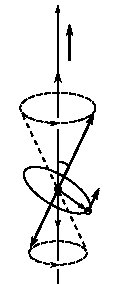
\includegraphics[width=0.15\textwidth]{v4_1}
    \caption{Прецессия электронной орбиты в магнитном поле}
    \figmark{electron orbit}
\end{wrapfigure}

Рассмотрим теперь случай, когда электрон исходно обладает некоторым
орбитальным моментом импульса $L=mvr$ и, соответственно,
магнитным моментом $\mu_L= \frac12 e v r$.
Пусть момент импульса $\vec{L}$ лежит в плоскости
рис.~\figref{electron orbit} и направлен под углом $\theta$ к некоторой оси $z$.
Орбитальное движение электрона эквивалентно витку с током,
магнитный момент которого $\vec{\mu}_L$ пропорционален $\vec{L}$
и направлен против него (поскольку заряд электрона отрицателен).
При включении внешнего магнитного поля с индукцией $B$,
направленной вдоль оси $z$, на электрон начинает
действовать момент силы $\vec{\mu}_L\times \vec{B}$,
перпендикулярный плоскости рис.~\figref{electron orbit} и направленны от
нас. Уравнение движения электрона будет иметь вид
\begin{equation*}
	\frac{d\vec{L}}{dt} = \vec{\mu}_L\times \vec{B}.
\end{equation*}
Как известно из механики, это уравнение описывает движение симметричного волчка
(гироскопа). Его решением является
прецессия электронной орбиты с угловой скоростью
$\omega_{L} = \frac{\mu_L B}{L}$,
направленной вдоль магнитного поля.
Подставляя значения $L$ и $\mu_L$, находим
$\omega_L = \frac{eB}{2m_e}$.
Таким образом, прецессия магнитного момента также происходит с ларморовской частотой
\eqref{Larmor-Omega}
и не зависит от угла $\theta$. Эта прецессия приводит
к дополнительному вращению электрона вокруг поля $B$,
налагающемуся на его орбитальное движение. Нетрудно убедиться, что она
даёт полностью аналогичный \eqref{chi-dia} вклад в диамагнитную восприимчивость.


% Сложно и ненужно // ППВ
%
% Если рассматривать сферически-симметричное распределение заряда
% электрона, то расчёт показывает, что $S = 2/3\pi\average{r^2}$, где
% $\average{r^2}$~--- средний квадрат расстояния электрона от ядра. Поэтому
% \begin{equation*}
% 	\Delta\mu = - \frac{\mu_0 e^2 \average{r^2}}{6m_e}H.
% \end{equation*}
%
% Появление этого момента и приводит к намагничиванию вещества в направлении,
% противоположном полю, т.е. к диамагнетизму. Магнитный момент атома, содержащего
% $Z$ электронов, находится суммированием магнитных моментов отдельных электронов:
% \begin{equation*}
% 	\mu_{\text{ат}} = - \frac{\mu_0 e^2 H}{6m_e}\sum\limits_{i=1}^Z
% \average{r_i^2}.
% \end{equation*}
%
% Сумму можно заменить произведением $Z\average{a^2}$, где $\average{a^2}$~---
% средний квадрат расстояния электронов от ядра. Тогда
% \begin{equation*}
% 	\mu_{\text{ат}} = - \frac{\mu_0 e^2 \average{a^2} Z}{6m_e}H.
% \end{equation*}
% Умножив полученное выражение на число атомов $n$ в единице объёма, получим
% намагниченность $M$:
% \begin{equation*}
% 	M = n\mu_{\text{ат}} = - \frac{\mu_0 e^2 \average{a^2} nZ}{6m_e}H.
% \end{equation*}
% Магнитная восприимчивость
% \begin{equation*}
% 	\chi = \frac{M}{H} = - \frac{\mu_0 e^2 \average{a^2} nZ}{6m_e}.
% \end{equation*}


Из полученного выражения \eqref{chi-dia} для восприимчивости диамагнетиков
следует, что она не зависит ни от температуры, ни от величины напряжённости поля
и растёт пропорционально порядковому номеру элемента.
Диамагнитный эффект свойствен всем веществам (независимо от того, имелся ли у
атома собственный магнитный момент или нет и как он был ориентирован), однако у
некоторых веществ он перекрывается более сильным \important{парамагнитным}
эффектом.


\labsection{Парамагнетизм}

Парамагнетизм характерен для веществ, частицы которых (атомы, ионы, молекулы)
обладают собственным магнитным моментом в отсутствие внешнего магнитного поля.

В парамагнетиках энергия взаимодействия между соседними магнитными моментами
атомов мала по сравнению с тепловой энергией,
поэтому в отсутствие внешнего магнитного поля магнитные моменты
являются полностью разупорядоченными, а намагниченность среды равна нулю.
При помещении во внешнее поле магнитным моментам энергетически выгодно
ориентироваться преимущественно по полю, что и приводит к парамагнитному эффекту.

% Ненужные подробности // ППВ
%
% Этот магнитный момент обусловлен как движением электронов в оболочке атома
% (орбитальный магнитный момент), так и наличием собственных магнитных моментов
% у электронов и ядер (\important{спиновый} магнитный момент).
% Например, в кристаллах медного купороса (CuSO$_4$) содержатся ионы меди,
% у которых электроны на внутренних оболочках имеют суммарный магнитный момент,
% не равный нулю. Изолированный атом меди имеет
% нечётное число электронов (29). На внешней оболочке $4s$ имеется всего один
% электрон, и именно его магнитный момент является магнитным моментом атома меди.
% Поэтому пары меди, как и пары натрия, являются парамагнетиками. Однако при
% переходе в твёрдое состояние (в процессе кристаллизации) атомы меди теряют этот
% электрон, он уходит от своего атома и уже принадлежит всему кристаллу.
% «Застывшие» в узлах решётки ионы меди уже не имеют магнитного момента и поэтому
% не обладают парамагнитным эффектом. Обобществлённые электроны (электроны
% проводимости) образуют электронный газ, который является парамагнетиком,
% поскольку состоит из частиц, обладающих собственным магнитным моментом. Такой
% парамагнетизм называют \important{парамагнетизмом Паули}. Но медь является
% диамагнетиком, и это означает, что диамагнетизм ионов меди преобладает над
% парамагнетизмом свободных электронов.

% Отличительной особенностью парамагнетиков является их слабая намагниченность во
% внешнем магнитном поле при комнатной температуре. В отсутствие магнитного поля
% энергия диполь-дипольного взаимодействия между двумя соседними магнитными
% моментами атомов с межатомным расстоянием $\sim 5 \cdot 10^{-8}$~см составляет
% $\sim 10^{-5}$~эВ, а энергия
% теплового движения на атом $\sim 7,5 \cdot 10^{-2}$~эВ. Такое превосходство
% тепловой энергии приводит к равномерному пространственному распределению
% магнитных моментов, а следовательно, к отсутствию намагниченности у
% парамагнетиков. Но когда начинает действовать внешнее магнитное поле, оно
% выстраивает магнитные моменты так, что магнитных моментов, направленных по полю,
% становится больше, чем направленных против поля, и с ростом поля намагниченность
% парамагнетиков растёт по закону \eqref{magnetization-magnetic vector}.
% Магнитная восприимчивость парамагнетиков всегда положительна, а по величине
% $\chi \sim 10^{-6} \sim 10^{-4}$~(система СИ).

% Упростим вывод до предела!

Оценим температурную зависимость магнитной восприимчивости парамагнетика
в классической модели. Пусть
среднее число атомов в единице объёма равно $n$, а абсолютная величина
магнитного момента атома $\mu_{\text{а}}$.
В магнитном поле с индукцией $B$ энергия магнитного диполя,
составляющего с направлением поля угол $\alpha$, равна
\begin{equation*}
	U = - \mu_{\text{а}}B \cos \alpha
\end{equation*}
и может меняться в диапазоне от $-\mu_{а}B$ до $+\mu_{а}B$
(квантовая механика говорит, что энергия может принимать
ряд дискретных значений в этом же диапазоне).

% \begin{wrapfigure}[]{r}{0.35\textwidth}
% \centering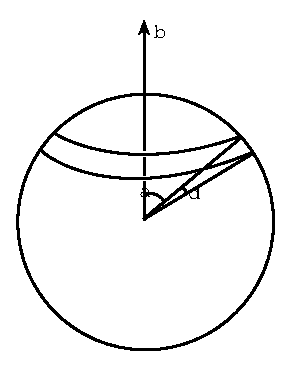
\includegraphics[width=0.2\textwidth]{v4_2}
% 	\caption{Телесный угол $d\Omega$.}
% 	\figmark{dN in dOmega}
% \end{wrapfigure}

Из термодинамики известно, что доля атомов, у которых момент ориентирован
под некоторым углом $\alpha$ к полю, определяется распределением Больцмана:
\begin{equation*}
    dn = \mathrm{const}\cdot  e^{-\tfrac{U(\alpha)}{\kB T}} d\alpha.
\end{equation*}
Пусть внешнее магнитное поле достаточно мало,
так что энергия магнитных моментов атомов в
нём много меньше тепловой: $\mu_{а}B \ll \kB T$.%
\footnote{Для оценки возьмём собственный магнитный момент электрона
$\mu_{e} = e\hbar/2m_e = 9,3 \cdot 10^{-24}\;Дж/Тл$
(магнетон Бора). В магнитном поле с индукцией $B = 1,0$~Тл магнитная энергия
$\mu_{e}~B \sim {10^{-4}}$~эВ --- такая энергия
соответствует температуре $T\sim 1\;К$.
Поэтому в не слишком больших полях и не слишком низких
температурах показатель больцмановской экспоненты действительно много меньше единицы.}
Число атомов, имеющих положительную ($\alpha > 0$) проекцию на направление $\vec{B}$ может
быть записана как
\[
n_{+} = n_0 e^{\mu_{а}B/\kB T}\approx n_0\left(1+\frac{\mu_{а} B}{\kB T}\right),
\]
где мы воспользовались разложением экспоненты от малого параметра,
а $n_0$ --- некоторая нормировочная константа. Для атомов с отрицательной
проекцией момента ($\alpha < 0$):
\[
n_{-} = n_0 e^{-\mu_{а}B/\kB T}\approx n_0\left(1-\frac{\mu_{а} B}{\kB T}\right)
\]
Здесь с учётом нормировки $n_{+} + n_{-} = n$, имеем $n_0 \approx n/2$.

Суммарный магнитный момент единицы объёма можно оценить как
\[
M \sim n_{+}\mu_{а} + n_{-}\cdot (-\mu_{а}) \approx
\frac{\mu_{а}^2 n}{\kB T} B.
\]
Более аккуратное усреднение по углам даст поправочный множитель порядка единицы
(в классической модели получается коэффициент $1/3$).

Таким образом, парамагнитная восприимчивость равна
\begin{equation}
    \eqmark{chi-para}
    \chi_{пар} \sim \frac{\mu_{\text{а}}^2 \mu_0 n}{3\kB T}\propto \frac{1}{T}.
\end{equation}
Температурная зависимость восприимчивости парамагнетиков вида~$\chi\propto 1/T$ называется
\important{законом Кюри}.

% Сложный вывод, при том нестрогий!
%
% Число атомов, магнитные моменты которых направлены под углами
% от $\alpha$ до
% $\alpha + d\alpha$ к полю, определяется распределением Больцмана:
% \begin{equation*}
%     dn = n_0 e^{-\tfrac{U}{\kB T}} \frac{d\Omega}{4\pi},
% \end{equation*}
% где $d\Omega = 2\pi\sin \alpha~d\alpha$ --- телесный угол, соответствующий интервалу
% $(\alpha;\alpha+d\alpha)$ (рис.~\figref{dN in dOmega}),
% $n_0$ -- нормировочная константа.
% Из условия нормировки находим
% \[
% n = n_0 \int\limits_0^\pi e^{\frac{\mu_{\text{а}} B \cos \alpha}{\kB T}}
% \sin \alpha~d\alpha.
% \]
% Полное число атомов в единице объёма
% \begin{equation}
% 	\eqmark{total number of atoms}
% 	N = 2\pi N_0 \int\limits_0^\pi e^{\frac{\mu_{\text{Б}} B \cos \alpha}{\kB T}}
% \sin \alpha~d\alpha.
% \end{equation}
% Проекция магнитного момента атома на направление поля равна
% $\mu_{\text{a}} \cos \alpha $, поэтому суммарный магнитный момент всех атомов единицы
% объема будет равен
% \[
% M = \int\limits_{0}^{\pi} \mu_{а} \cos \alpha dn.
% \]
% Вычисления сильно упрощаются, если энергия атома в магнитном поле мала по сравнению
% с тепловой энергией $\mu_{а} B \ll \kB T$. Тогда, если воспользоваться разложением
% экспоненты $e^{-U/\kB T}\approx 1 + \frac{U}{\kB T}$, нетрудно получить:
% \begin{equation}
% \eqmark{total magnetic moment}
% %
% % n_0 \int\limits_0^\pi \mu_{\text{а}} \cos \alpha \exp
% % \left(\frac{\mu_{\text{а}} B \cos \alpha}{\kB T}\right) \sin \alpha~d\alpha.
% \end{equation}
% В этом приближении из совместного решения \eqref{total number of atoms} и
% \eqref{total magnetic moment} получим, что намагниченность


В сверхсильных полях, когда магнитная энергия внутриатомного диполя сравнима с
тепловой ($B \sim 10^3$~Тл при комнатной температуре), все магнитные моменты в
парамагнетике могут ориентироваться по полю~--- наступает \important{магнитное насыщение}.

В случае парамагнетизма свободных электронов, образующих электронный газ в
металлах, не все электроны могут участвовать в переориентировке своих магнитных
моментов, а только небольшая часть, которая пропорциональна тепловой энергии
$\kB T$ (квантовый эффект). Поэтому у некоторых металлов парамагнетизм не зависит
от температуры.

\labsection{Ферромагнетизм}

Помимо диа- и парамагнетиков, которые слабо реагируют на внешнее магнитное поле,
в природе существуют вещества, способные сильно намагничиваться даже в небольших
магнитных полях. Такие вещества относят к классу ферромагнетиков. Это~---
железо, никель, кобальт, гадолиний и многочисленные сплавы этих металлов между
собой и с другими металлами. Ферромагнитными свойствами обладают некоторые
сплавы элементов, которые порознь не являются ферромагнитными (например, сплавы
меди и марганца), и ряд неметаллических веществ (ферриты). Ферромагнитные явления
сложны и многообразны, и мы ограничимся изложением лишь некоторых основных фактов.

Зависимость намагниченности $M$ от напряжённости магнитного поля $H$ у всех
ферромагнетиков оказывается нелинейной: магнитная восприимчивость
$\chi=\chi(H)$ у ферромагнетиков не является константой и зависит от $H$.
Если у диа- и парамагнетиков $\chi$ составляет всего $10^{-8}$~--~$10^{-4}$, то у
ферромагнетиков магнитная восприимчивость достигает значений $10^3$~--~$10^4$.
Кроме того, у ферромагнетиков (особенно монокристаллических)
магнитная восприимчивость $\chi$ может иметь тензорный характер
(векторы $\vec{M}$ и $\vec{H}$ не сонаправлены),
обусловленный анизотропией кристаллической решетки.

% Этому место в начале раздела // ППВ
%
% Степень намагничивания ферромагнитного вещества можно
% характеризовать не только вектором намагниченности $M$, но и вектором магнитной
% индукции $B$ в данном веществе:
% \begin{equation*}
% 	B =\mu_0 (H + M).
% \end{equation*}
% При $M = \chi H$
% \begin{equation}
% 	B = \mu_0 (1 + \chi)H = \mu \mu_0 H.
% \end{equation}
% \todo [author=Tiffani]{В формуле 4.4 была ошибка. Исправила.}
%
% Величина $\mu = 1+ \chi$ носит название магнитной проницаемости вещества. Если у
% диа- и парамагнетиков $\mu$ отличается от единицы всего на сотые доли процента,
% то у ферромагнетиков $\mu$ практически совпадает с $\chi$ (в системе СИ).
%
% Отметим, что в системе СГС, где $B = (1 + 4\pi \chi) H$, $\chi$ в $4\pi$ раз
% меньше, чем в системе СИ.

Как и в случае парамагнетиков, атомы ферромагнетика обладают собственным магнитным
моментом. Однако даже в отсутствие внешнего магнитного поля атомы ферромагнетика
способны образовывать упорядоченные структуры (\important{домены}),
в которых все магнитные моменты ориентированы практически в одном направлении.
Таким образом, каждый отдельный атом испытывает влияние не только внешнего
поля, но и поля, созданного ``дружным коллективом'' его соседей.
В качестве простейшей эмпирической модели, описывающей такую ситуацию, можно
рассмотреть
так называемую модель \important{среднего поля}: предположим, что намагниченность
элемента среды пропорциональна некоторому эффективному полю $H_{эфф}$
складывающемуся из поля $\vec{H}$ в данной точке, созданного сторонними токами, и среднего ``коллективного'' поля,
пропорционального величине намагниченности $\vec{M}$:
\begin{equation}
\eqmark{average-field}
\vec{M} = \chi_{пар} \vec{H}_{эфф},\qquad \vec{H}_{эфф} = \vec{H} + \beta \vec{M},
\end{equation}
где $\chi_{пар}$ --- парамагнитная восприимчивость отдельного атома
\eqref{chi-para}, $\beta$~--- некоторая безразмерная константа, определяемая из опыта.

Модель среднего поля позволяет уточнить закон Кюри.
Определяя магнитную восприимчивость по-прежнему как $\chi = M/H$, найдём
из \eqref{average-field}:
\begin{equation}
    \eqmark{Kuri-Weiss}
    \chi = \frac{1}{\frac{1}{\chi_{пар}}-\beta} \propto
    \frac{1}{T-\Theta},
\end{equation}
где параметр $\Theta = \beta \frac{\mu_{a}^2\mu_0 n}{3\kB}$ имеет размерность
температуры.

Соотношение \eqref{Kuri-Weiss} называют
\important{законом Кюри--Вейсса}. В частности, этот закон предсказывает
существование особой точки, в которой $\chi$ обращается в бесконечность.
Действительно, существует температура $\Theta_К$, называемая
\important{точкой Кюри}, в которой имеет место фазовый переход (2-го рода) между
парамагнитным (при $T>\Theta_К$) и ферромагнитным состоянием среды
при $T < \Theta_К$. Закон Кюри--Вейсса удовлетворительно выполняется
вдали от $\Theta_К$, однако нарушается при приближении к точке перехода
$T \to \Theta_К$, где модель среднего поля становится слишком груба.
Поэтому параметр $\Theta$ в \eqref{Kuri-Weiss} несколько
отличается от температуры Кюри: как правило, $\Theta_К < \Theta$.

Остановимся кратко на причине, по которой соседним магнитным моментам выгодно
объединяться в домены. В первую очередь подчеркнём, что
магнитное (диполь-дипольное) взаимодействие между атомами
не может привести к упорядочению системы.
Чтобы в этом убедиться, достаточно оценить энергию такого взаимодействия:
из квантовой механики известно, что магнитный момент атома
по порядку величины равен~$\mu_Б = 9,3\cdot 10^{-24}\; Дж/Тл$
(\emph{магнетон Бора}),
характерное расстояние между атомами~$a\sim 2 \cdot 10^{-10}\;м$,
тогда характерное межатомное магнитное поле
$B \sim \mu_0 \frac{\mu_Б}{a^3} \sim 1\;Тл$, и характерная энергия
энергия диполь-дипольного взаимодействия
$U_{дип.}\sim \mu_Б B \sim 10^{-4}\;эВ$.
При такой энергии связи тепловое движение обеспечит полное
разупорядочение уже при $T\sim 1\;К$.

Единственное взаимодействие, которое способно выстроить в ряд магнитные
моменты электронов в атомах при температурах порядка комнатной, --- это
\emph{электростатическое} взаимодействие
(его энергия на несколько порядков больше магнитной:
$e^2/(4\pi\varepsilon_0 a) \sim 1\;эВ$).
Как следует из квантовой механики, если магнитные моменты (или спины) электронов
соседних атомов сонаправлены,
их электростатическое отталкивание становится \emph{меньше}.
Таким образом, магнитным моментам атомов энергетически выгодно ориентироваться
в одном направлении. Такое явление получило название
\important{обменного взаимодействия}.

% Написано крайне не аккуратно // ППВ
%
% Учёт взаимодействия
% элементарных магнитных моментов, заключающийся в прибавлении к макроскопическому
% полю $H$ поля, пропорционального намагниченности (подобно приёму учёта поля
% соседей в диэлектрике введением поля поляризуемости с коэффициентом $4\pi/3$),
% противоречит опыту, поэтому вводится эмпирическая постоянная $\lambda$, т.е.
% вместо поля $H$ нужно использовать величину $H + \lambda M$.  Используя
% полученную формулу для намагниченности, получим
% \begin{equation*}
% 	M = \frac{\mu_{\text{Б}}^2 \mu_0 N}{3\kB T}(H + \lambda M)
% \end{equation*}
% и соответственно
% \begin{equation*}
% 	\chi = \frac{\mu_{\text{Б}}^2 \mu_0 N}{3k(T - \Theta)},
% \end{equation*}
% где $\Theta = \mu_{\text{Б}}^2 \mu_0 N / 3k$ имеет размерность температуры.

% Зависимость  $1/\chi$  от температуры называется законом Кюри-Вейса и
% представляется прямой, пересечение которой с осью абсцисс определяет
% характеристическую температуру. Если эта величина положительна, существует
% температура, ниже которой восприимчивость принимает огромные значения. Это
% справедливо для ферромагнетиков, остальные вещества ведут себя подобным образом
% вблизи абсолютного нуля. Для $T>\Theta$ ферромагнетики ведут себя как
% парамагнетики.

% Результаты экспериментов для постоянной $\lambda$ для ферромагнетиков дают
% величину $10^4$, т.е.поле, пропорциональное намагниченности, оказывается порядка
% $10^7$~эрстед (хотя поле соседних узлов решетки около $10^3$~эрстед).

% Огромная величина поля, связанная с намагниченностью, нашла своё объяснение в
% квантовой теории при введении так называемого обменного взаимодействия
% электронов, т.е. эти силы имеют электростатическую природу. Характерная энергия
% этого взаимодействия порядка $10^{-13}$~эрг. В результате этого взаимодействия
% устойчивое состояние ферромагнетика соответствует полной намагниченности, хотя в
% реальности   оказываются намагничены микроскопические области размером порядка
% несколько микрометров, а в целом образец ненамагничен. Следует  отметить, что
% величина магнитного поля в домене примерно совпадает с полем насыщения
% ферромагнетика. Области полной намагниченности назвали доменами, размер которых
% является следствием конкурирующих вкладов в полную энергию ферромагнетика:
% обменной энергии, энергии анизотропии и магнитной энергии. Пример разбиения
% кристалла на домены приведён на рисунке (??4.3.1??), где полная энергия
% уменьшается от a) до в).
% \todo [author=Tiffani]{Присутствует ссылка на рис. 4.3.1, которого нет в папке.
% См. примечание ниже.}
%
% \todo [author=Tiffani]{Здесь должна быть картинка 4.3.1, но она не соответствует
% той, что в ворде. Нужную картинку в папке с картинками не нашла.}

\begin{wrapfigure}[]{r}{0.4\textwidth}
    \centering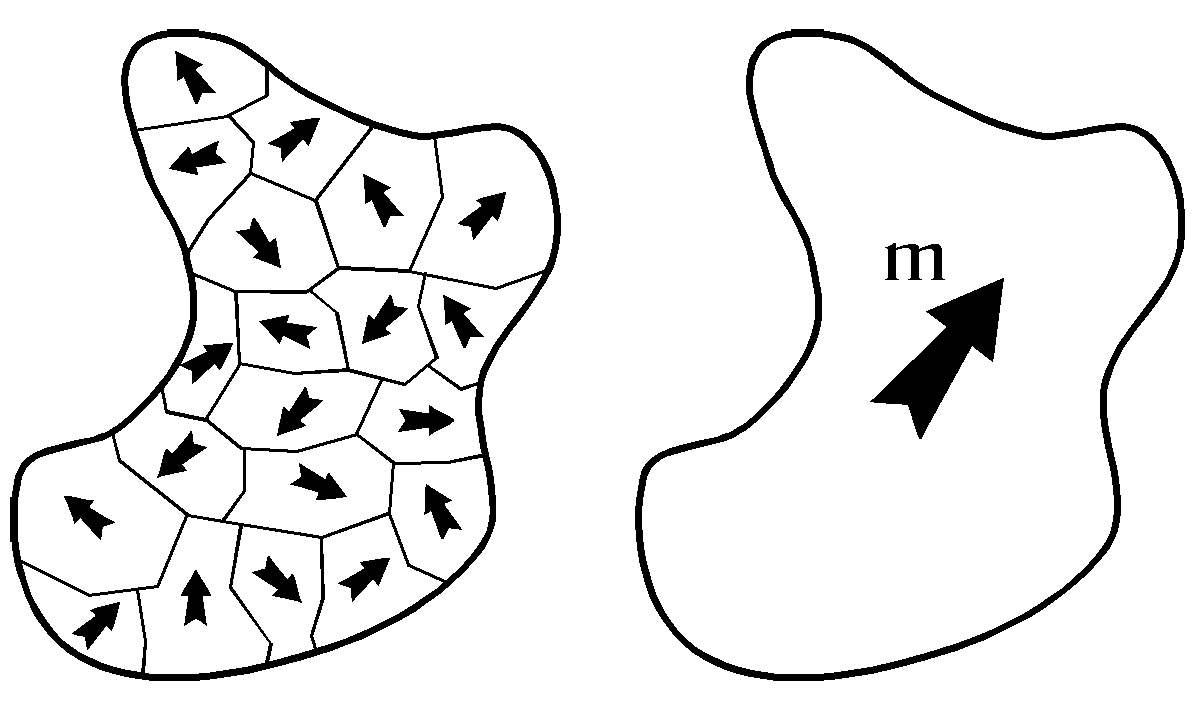
\includegraphics[width=0.35\textwidth]{Chapter_4/domains}
    \caption{Доменная структура ферромагнетика при слабом (слева)
    и сильном (справа) внешнем поле}
    \figmark{domains}
\end{wrapfigure}

С другой стороны, магнитное диполь-дипольное взаимодействие между доменами препятствуют
выстраиванию всех магнитных моментов среды в одном направлении.
Действительно, энергия такого взаимодействия будет минимальной
при \emph{анти}параллельном расположении магнитных моментов соседних элементов среды.
Поэтому при определённом поперечном размере домена оказывается
энергетически выгодно иметь соседний домен с противоположно ориентированным моментом
(см. рис.~\figref{domains}, слева).
Наложение внешнего поля заставляет домены ориентироваться
по нему, что приводит к резкому увеличению намагниченности образца, а при
достаточно большом поле достигается состояние \important{насыщения},
когда все домены ориентируются по полю (см. рис.~\figref{domains}, справа).

% Между доменами существуют переходные слои (в железе их толщина $\sim
% 10^{-5}$~см), в которых направление магнитного момента атомов плавно переходит
% от направления в одном домене к направлению в соседнем. Такие слои называют
% «стенками Блоха». Энергия этих слоёв пропорциональна их площади.
% \todo [author=Tiffani]{Неплохо было бы выделять термины вроде «стенками Блоха» и
% «скачки Баркгаузена» курсивом или жирным шрифтом при первом упоминании в
% тексте.}

\labsection{Ферромагнитный гистерезис}

Если состояние некоторой системы зависит не только от мгновенных значений
внешних параметров, но от истории их изменений, говорят, что
в системы имеет место \important(гистерезис).

Именно такими свойствами обладает магнитный момент ферромагнитного образца
как функция напряжённости поля $M(H)$. В частности,
система может оказаться намагниченной, даже когда внешнее поле выключено ---
этим объясняется существование постоянных магнитов. Рассмотрим данное явление подробнее.

Пусть ферромагнетик находится исходно в ненамагниченном состоянии
($M = 0$). Медленно увеличивая поле $H$ в образце, получим зависимость
$M(H)$, которую называют \emph{начальной кривой намагничивания}. Эту кривую обычно
разделяют на пять условных участков (рис.~\figref{magnetization curve}).

Участок 1~--- область обратимого намагничивания, где $M =\chi H$. В этой области
происходят процессы упругого смещения границ доменов: увеличивается размер тех
доменов, магнитный момент которых близок к направлению магнитного поля, и
уменьшаются размеры доменов с противоположным направлением магнитного момента.

\begin{wrapfigure}[]{r}{0.5\textwidth}
    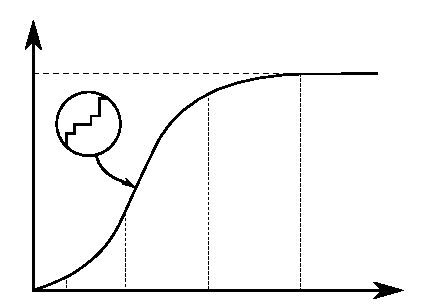
\includegraphics[width=0.4\textwidth]{v4_3}
    \caption{Начальная кривая намагничивания ферромагнетика}
    \figmark{magnetization curve}
\end{wrapfigure}

Участок 2 характеризуется квадратичной зависимостью $M$ от $H$. В этой области
также идёт процесс обратимого смещения границ, но проявляется нелинейный характер
зависимости намагниченности от поля.

Область максимальной скорости роста намагниченности 3 соответствует необратимым
смещениям стенок между доменами (<<стенок Блоха>>):
им приходится преодолевать <<препятствия>> в виде примесей,
дислокаций и дефектов кристаллической решётки.
Когда стенка наталкивается на такое препятствие, она останавливается и держится,
пока поле не достигнет порогового значения, при котором она внезапно
срывается. Таким образом, движение доменной стенки приобретает скачкообразный
характер (<<скачки Баркгаузена>>).

% Фрагмент кривой намагничивания в этой области в увеличенном масштабе показан на
% рис.~\figref{magnetization curve}. Скачкообразное движение стенок приводит к
% быстрому изменению намагниченности образца, что вызывает появление вихревых
% токов, а следовательно, диссипацию энергии. Выделение тепла внутри образца и
% приводит к необратимому движению доменных стенок.

В достаточно сильных полях движение стенок прекращается и энергетически
выгодным становится поворот магнитных моментов тех оставшихся доменов, у которых
магнитный момент не совпадает с направлением поля (область 4).

И, наконец, при некотором значении поля (участок 5) все магнитные моменты
выстраиваются по полю~--- намагниченность образца достигает \emph{насыщения}.

% Повторы! // ППВ
%
% \begin{wrapfigure}[12]{r}{0.35\textwidth}
% 	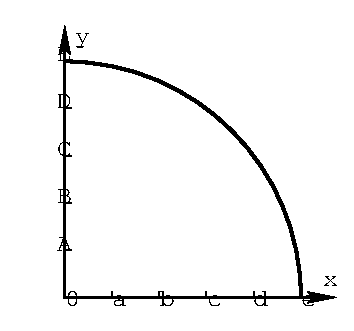
\includegraphics[width=0.2\textwidth]{v4_4}
% 	\caption{Зависимость намагниченности насыщения ферромагнетика от
% температуры}
% 	\figmark{magnetization-temperature}
% \end{wrapfigure}
%
% Магнитные и другие физические свойства ферромагнетиков существенным образом
% зависят от температуры. Например, намагниченность насыщения $M_s$ имеет
% наибольшее значение при $T = 0~(M_s (0))$ и монотонно уменьшается до нуля при
% температуре $\Theta$, которую называют ферромагнитной точкой Кюри
% (рис.~\figref{magnetization-temperature}).
%
% \todo [author=Tiffani]{Обозначения на рис. 4.4 не имеют ничего общего с
% действительностью.}
%
% Выше  этой температуры $\Theta$ тепловое движение разупорядочивает магнитную
% структуру доменов и ферромагнетик переходит в парамагнитное состояние. В
% отсутствие внешнего магнитного поля переход ферромагнетик~---парамагнетик
% является фазовым переходом II рода.
%
% Мы уже знаем, что для парамагнетиков зависимость магнитной восприимчивости от
% температуры имеет вид закона Кюри ($\chi \sim 1/T$). Аналогичная зависимость
% восприимчивости ферромагнетиков от температуры при температурах выше $\Theta$
% описывается законом Кюри-Вейсса:
% \begin{equation*}
% 	\chi = \frac{C}{T - \Theta_p},
% \end{equation*}
% где $C$ -- постоянная Кюри, $\Theta_p$ -- температура Кюри (как правило
% $\Theta_p > 0$).

На практике магнитные свойства ферромагнетиков обычно изучают путём измерения
зависимости индукции магнитного поля $B(H)$ от напряжённости магнитного поля $H$ в
веществе. Исследование образца, естественно, начинают с полностью
размагниченного состояния ($H = 0$, $B = 0$). Если теперь монотонно увеличивать
напряжённость поля $H$, то изменение $B$ происходит по рассмотренной выше
начальной кривой намагничивания с учётом соотношения \eqref{fieldB}
(кривая $OA$ на рис.~\figref{hysteresis curve}).

Наклон кривой намагничивания принято характеризовать
\important{дифференциальной} магнитной проницаемостью
\begin{equation}
    \eqmark{mu-diff}
    \mu_{\text{дифф}} \equiv \frac{1}{\mu_0} \frac{dB}{dH}.
\end{equation}
С ростом $H$ величина $\mu_{дифф}$ сначала растёт (участки 1 и 2),
затем с середины участка 3 начинает резко падать,
приближаясь к единице при насыщении.

\begin{wrapfigure}{r}{0.4\textwidth}
    \pic{0.38\textwidth}{v4_8}
    \caption{Начальная кривая намагниченности и кривая гистерезиса}
    \figmark{hysteresis curve}
\end{wrapfigure}

Доведём систему до некоторой точки $A$, лежащей в области
насыщения (здесь $B_s$~--- \important{индукция насыщения}\footnote[1]{s~--- saturated
(англ.)~--- насыщенный}), и начнём уменьшать напряжённость поля $H$.
Поскольку между доменами есть трение, обратный путь
пойдёт не по начальной кривой, а выше неё.

При выключения внешних полей, то есть при достижении $H = 0$,
в образце сохраняется некоторое собственное намагничивание.
Соответствующее значение индукции $B_r$
называют \important{остаточной индукцей}\footnote[2]{r~--- remained (англ.)~--- оставшийся}.

Значение $B = 0$ достигается лишь при некотором отрицательном значении
$H = - H_c$. Величина $H_c$ называется
\important{коэрцитивным полем}\footnote[3]{c~--- coercive (англ.)~--- принудительный}.
Среди ферромагнетиков принято различать \emph{магнитожёсткие}
(с $H_c > 10^3$~А/м) и \emph{магнитомягкие матералы}. В точке $C$
наступает насыщение для намагничивания в противоположную сторону.

Если теперь попробовать вернуться в точку $A$, вновь наращивая поле,
получим некоторый замкнутый цикл (\important{кривую гистерезиса}). Если
в точке $A$ насыщение не достигается, то аналогичным образом можно получить
цикл меньшей площади (заметим, что поскольку процессы, происходящие
в системе, необратимы, цикл будет вообще говоря незамкнутым).

Отметим, что \emph{площадь петли} гистерезиса ферромагнетика на плоскости
$H$--$B$ есть энергия, необратимо выделяющейся в виде тепла в единице
объёма вещества за один цикл:
\begin{equation}
    \eqmark{HdB}
    \Delta w = -\oint {HdB}
\end{equation}
(см. далее вывод формулы \eqref{magnetic-energy}).

% Можно короче. // ППВ
%
% Магнитное состояние вещества
% характеризуется теперь точками кривой $CA$, лежащими низке начальной кривой
% намагничивания. Строго говоря, кривая не пройдёт и через точку $A$, а окажется
% ниже неё. Вновь уменьшая магнитное поле, мы пройдём поэтому по кривой,
% расположенной ниже кривой $AC$, не попадём в точку $C$ и начнём движение к $A$
% по некоторому новому пути. Магнитные циклы, таким образом, обычно оказываются
% незамкнутыми. Многократно проходя один и тот же цикл, образец приближается к
% предельному замкнутому циклу (кривой гистерезиса), не зависящему от начального
% состояния. Описанная картина наиболее отчётливо проявляется в тех случаях, когда
% образец не доводится до насыщения. При заходе в область насыщения намагничивание
% зависит главным образом от $H$ и лишь в очень слабой степени от истории образца.
% Предельные циклы устанавливаются при этом сразу (т. е. при однократном
% прохождении цикла) или почти сразу. В соответствии с этим на
% рис.~\figref{magnetization curve} не сделано различия между частным циклом и
% предельным.


\labsection{Измерение напряжённости и индукции магнитного поля}

\paragraph{Размагничивающий фактор.}
Когда говорят о кривой намагничивания $B(H)$,
речь идёт о \emph{локальной} связи между
индукцией и напряжённостью магнитного поля в каждой точке среды.
При этом под $H$ имеется в виду не внешнее магнитное поле,
а именно поле \emph{внутри} данного материала. Поскольку непосредственному
измерению легче всего поддаётся именно внешнее поле $\vec{H}_{0}$,
создаваемое сторонними токами без образца, необходимо установить связь
между $\vec{H}$ и $\vec{H}_0$ (заметим, что $\vec{B}_0=\vec{H}_0$).

Из условия непрерывности касательной компоненты вектора $\vec{H}$ следует,
что $\vec{H}$ совпадает $\vec{H}_{0}$ только если во всех точках образца
$\vec{H} \parallel \vec{H}_{0}$.
Такое возможно, например, в пределе \emph{бесконечно длинного соленоида} либо
для \emph{тонкого тора}.
В общем случае $\vec{H}_0 \ne \vec{H}$.

Рассмотрим магнетик, помещённый в однородное внешнее поле $\vec{H}_0$.
Разность между внешним полем и полем в образце принято называть
\important{размагничивающим полем}:
$\vec{H}_{разм} = \vec{H}_0 - \vec{H}$.
Если форма образца такова, что его намагниченность можно считать
практически постоянной $\vec{M}\approx\mathrm{const}$ (за исключением,
возможно, незначительных ``краевых эффектов''), можно ввести
коэффициент пропорциональности между $\vec{H}_{разм}$ и намагниченностью $\vec{M}$,
называемый \important{размагничивающим фактором}:
\[
N_{разм} = \frac{H_0-H}{M}.
\]
Для однородного образца размагничивающий фактор зависит
только от его формы и ориентации в поле.
С учётом \eqref{fieldB} нетрудно убедиться, что его величина может меняться в пределах $0\le N_{разм} \le 1$.

Для образца с известным $N_{разм}$, изготовленного из материала
c проницаемостью $\chi$, помещённого во внешнее поле $H_0$, имеем
$H_0 - H = N M$, $M=\chi H$, откуда
\[
M = \frac{\chi H_0}{1+N_{разм}\chi}.
\]

Аналитические выражения для $N_{разм}$ могут быть получены только для тел
простейшей формы. В частности
\begin{itemize}
    \item бесконечно длинный цилиндр: продольное поле~--- $N_{разм} = 0$,
          поперечное поле~--- $N_{разм} = 1/2$;
    \item шар $N_{разм} = 1/3$;
    \item бесконечно тонкая пластинка в поперечном поле $N_{разм} = 1$,
          в продольном --- $N_{разм} = 0$.
\end{itemize}

Заметим, что для диа- и парамагнетиков $|\chi|\ll 1$, поэтому отличием $H$ от
$H_0$ для них можно, как правило, пренебречь.

% Сложно и ненужно // ППВ
%
% На практике
% для снятия петли гистерезиса мы обычно помещаем во внешнее однородное магнитное
% поле ферромагнитный образец, имеющий конечные размеры. Однородная
% намагниченность по всему объёму образца будет иметь место только для образцов,
% имеющих форму эллипсоидов вращения, в частности, для шара, для очень тонкой
% пластинки и для тонкого и длинного цилиндра. Во всех этих случаях величина
% магнитного поля внутри образца будет меньше внешнего магнитного поля. Рассмотрим
% в качестве примера образец, имеющий форму цилиндра длиной $l$ и диаметром $d (d
% \ll l)$.
%
% Пусть ось симметрии цилиндра направлена вдоль внешнего магнитного поля величиной
% $H_0$. Цилиндр будет практически однородно намагничен с некоторой
% намагниченностью $M$. Найдём величину индукции магнитного поля на оси цилиндра в
% точке, равноудалённой от торцов. С одной стороны, используя связь между $B$, $M$
% и $H$, можно записать
% \begin{equation}
% 	\eqmark{cylinder-B(H)}
% 	B_{\text{вн}} = \mu_0 (H_{\text{вн}} + M),
% \end{equation}
% где $H_{\text{вн}}$~--- величина поля внутри образца. С другой стороны,
% намагниченный цилиндр можно рассматривать как цилиндрическую поверхность
% диаметра $d$ с однородным кольцевым поверхностным током плотностью:
% \begin{equation*}
% 	j = M.
% \end{equation*}
% Эти молекулярные токи создают собственное магнитное поле, которое по направлению
% совпадает с внешним полем $H_0$, а по величине равно\footnote[4]{См. [4]. Задача
% № 5.5.}:
%
% \todo [author=Tiffani]{Возможно, лучше вместо ``См. [4]. Задача № 5.5.''
% написать ``См. в приложении'', т.к. задача будет в приложении к этой главе}
% \begin{equation*}
% 	H_{\text{мол}} = \frac{Ml}{\sqrt{l^2 + d^2}}.
% \end{equation*}
%
% Индукцию магнитного поля найдём как суперпозицию внешнего поля и поля
% молекулярных токов:
% \begin{equation}
% 	\eqmark{B(H)-molecular current}
% 	B_{\text{вн}} = \mu_0\left( H_0 + \frac{Ml}{\sqrt{l^2 + d^2}} \right).
% \end{equation}
% Приравнивая \eqref{cylinder-B(H)} и \eqref{B(H)-molecular current}, получим
% \begin{equation*}
% 	H_0 + \frac{Ml}{\sqrt{l^2 + d^2}} = H_{\text{вн}} + M.
% \end{equation*}
%
% Разность между внешним и внутренним полями называют размагничивающим полем:
% \begin{equation*}
% 	H_{\text{разм}} = H_0 - H_{\text{вн}} = \left( 1 - \frac{1}{\sqrt{1 + \left(
% \frac{d}{l} \right)^2}} \right) M = N_p M.
% \end{equation*}
% И тогда связь поля внутри и поля внешнего
% \begin{equation*}
% 	H_{\text{вн}} = \frac{H_0}{1 + N_p M},
% \end{equation*}
% а  магнитная проницаемость образца
% \begin{equation*}
% 	\chi_{\text{обр}} = \frac{\chi}{1 + N_p \chi}.
% \end{equation*}
% \important{Коэффициент пропорциональности между размагничивающим полем и
% намагниченностью образца обозначают через $N_p$ и называют размагничивающим
% фактором или коэффициентом размагничивания. Его величина зависит только от
% геометрических размеров образца и может изменяться в пределах от 0 до 1.}

% Полученное выражение для $N_p$ цилиндра с параметрами $d/l \ll 1$ всё равно
% остаётся приближённым выражением, хотя и с достаточно хорошим приближением. А
% вот точные значения размагничивающего фактора могут быть рассчитаны только в
% отдельных частных случаях:

\paragraph{Измерения в тороидальном образце.}

\begin{wrapfigure}[13]{r}{0.4\textwidth}
    \pic{0.38\textwidth}{v4_5}
    \caption{Тороидальный образец с намагничивающей обмоткой}
    \figmark{toroid}
\end{wrapfigure}

В лабораторных условиях для исследования зависимости $B(H)$ ферромагнитных
материалов обычно используют образцы тороидальной формы. Если на тор намотать
равномерную намагничивающую обмотку (рис.~\figref{toroid}), то поле $H$ внутри
тора на окружности радиуса $R$ будет пропорционально току $I$ в обмотке, а его
величину можно рассчитать по теореме о циркуляции вектора $H$:
\begin{equation}
    \eqmark{H-toroid}
    H = \frac{IN_0}{2\pi R},
\end{equation}
где $N_0$~--- число витков намагничивающей обмотки. Напряжённость магнитного
поля в тороидальном образце зависит от $R$, поэтому
намагниченность образца можно считать однородной при $r \ll R$, где $r$ ---
радиус сечения тора.

\begin{wrapfigure}{r}{0.4\textwidth}
    \pic{0.38\textwidth}{v4_6}
    \caption{Тороидальная катушка с разрезом}
    \figmark{toroidal coil-cut}
\end{wrapfigure}

\paragraph{Поле в зазоре электромагнита.}
Рассмотрим теперь тороидальную катушку, в которой сделан узкий разрез толщиной
$\delta$ ($\delta \ll r \ll R$) (рис.~\figref{toroidal coil-cut}).

Пусть $H_1$~--- напряжённость магнитного поля в
образце, а $H_2$~--- в зазоре. По теореме о циркуляции вектора $H$ имеем
\begin{equation}
	\eqmark{H-toroid-cut}
	\oint {Hdl} = H_1 (2\pi R - \delta) + H_2 \delta  = N_0 I.
\end{equation}

Воспользуемся нeпрерывностью нормальных составляющих вектора магнитной
индукции $B$ на границах разреза. В образце имеем $B_1 = \mu_0 \mu H_1$,
а в зазоре $B_2 = \mu_0 H_2$, поэтому приравнивая $B_1$ и $B_2$, найдём:
\[H_2 = \mu H_1.\]
Подставляя это в \eqref{H-toroid-cut}, получим
\begin{equation}
	\eqmark{H1-toroid-inside}
	H_1 = \frac{N_0 I}{2\pi R + (\mu - 1)\delta},\quad H_2 = \mu H_1
\end{equation}
Отметим, прежде всего, что напряжённости поля в образце и в зазоре
(при $\mu = \mathrm{const}$) пропорциональны силе намагничивающего тока.
После того, как установлена величина коэффициента
пропорциональности, измерение напряжённости может быть заменено измерением тока.

При наличии даже небольшого зазора второе слагаемое в знаменателе
\eqref{H1-toroid-inside} может существенно превосходить первое из-за большой величины
$\mu\gg1$. Тогда полагая $\mu\gg \frac{2\pi R}{\delta}\gg 1$, из
\eqref{H-toroid-cut} найдём поле в зазоре:
\begin{equation}
	\eqmark{H2-toroid-big gap}
	H_2 \approx \frac{N_0 I}{\delta}.
\end{equation}
Интересно, что из \eqref{H2-toroid-big gap} следует, что поле в зазоре
электромагнита практически не зависит ни от размеров и формы магнитного ярма (части
магнитной цепи, заполненной веществом с большим $\mu$), ни от его материала.

% Воздушные зазоры электромагнитов можно использовать для исследования
% ферромагнитных образцов. А можно и не использовать.


\paragraph{Измерение индукции в образце.}
Одни из простейших и в то же время надёжных методов измерения
индукции $B$ внутри некоторого образца основан
на законе электромагнитной индукции.
Электродвижущая сила, возникающая в контуре при изменении
пронизывающего контур магнитного потока $\Phi(B)$, равна
\begin{equation}
	\eqmark{EMF-magnetic flux}
	\mathcal{E} = - \frac{d\Phi (B)}{dt},
\end{equation}
Так как магнитный поток $\Phi (B)=BS$ равен произведению индукции $B$ на площадь
образца $S$, формула \eqref{EMF-magnetic flux} позволяет определить производную от
индукции $B$. Чтобы измерить саму величину $B=-\frac1{S}\int \mathcal{E} dt$,
необходимо иметь некоторое интегрирующее устройство.
В качестве такового может быть применён милливеберметр (работа 3.4.1),
баллистический гальванометр (работа 3.4.4), интегрирующая $RC$-цепочка
(работа 3.4.5). В современной практике всё чаще применяется цифровое интегрирование.

Следует обратить внимание, что при измерениях в переменном поле
в образцах с большим $\mu$ и хорошей электропроводностью
нельзя не учитывать конечную глубину
проникновения поля в образец (\emph{скин-эффект}), равную%
\footnote{См. \textit{Сивухин Д.В.} Общий курс физики, Т.~3, \S 144.}
\[
\delta \sim \sqrt{\frac{\rho}{\mu \mu_0 f}},
\]
где $\rho$ --- удельное сопротивление, $f$ --- частота колебаний поля.
Например, при $f=50\;Гц$ для чистого железа ($\rho \approx 10^{-7}\;Ом\cdot м$,
$\mu \sim 10^3$) имеем $\delta \sim 1\;мм$.


\labsection{Энергия и силы в магнитном поле}

\paragraph{Энергия поля.}
Рассмотрим соленоид длиной $l$, площадью $S$ и числом витков $N$,
заполненный магнетиком с известным законом зависимости индукции от напряжённости
поля $B(H)$ (или $H(B)$). Подключим соленоид к источнику $\mathcal{E}$.
Пусть омическое сопротивление цепи равно $R$.
Плавно (квазистатически) увеличим ток в цепи до некоторого значения
$I$, так что напряжённость в соленоиде станет равна
$H = \frac{N}{l} I$. Закон Ома в цепи соленоида имеет вид
\begin{equation}
    \eqmark{OhmLaw-solenoid}
\mathcal{E} - IR = \frac{d\Phi}{dt},
\end{equation}
где правая часть отвечает ЭДС индукции, $\Phi = NBS$ --- магнитный поток в
цепи.

Магнитная энергия $W_М$, запасённая в соленоиде, равна работе
источника $A_{ист}=\int \mathcal{E}I\, dt$ за вычетом тепловыделения $Q=\int I^2 R\, dt$.
С~учётом \eqref{OhmLaw-solenoid}, получим
\begin{equation}
    \eqmark{magnetic-energy-full}
W_М = \int\limits_0^t I(\mathcal{E} - I R) dt =
\int\limits_0^t I\frac{d\Phi}{dt} dt = \int I\,d\Phi.
\end{equation}
В последнем равенстве мы перешли от интегрирования
по времени к интегрированию по значениям $\Phi$. Если связь между потоком и током
\emph{линейна}: $\Phi = L I$, где $L=\mathrm{const}$ --- индуктивность, то
справедлива обычная формула для магнитной энергии
\begin{equation}
    \eqmark{magnetic-energy-full-simple}
    W_М = \frac{LI^2}{2} = \frac{\Phi I}{2} = \frac{\Phi^2}{2 L}.
\end{equation}


В случае произвольной геометрии магнетик
можно разбить на элементарные ячейки и определить
\important{объёмную плотности энергии} магнетика: разделив
\eqref{magnetic-energy-full} на объём $V=Sl$ и воспользовавшись соотношениями
$\Phi = NBS$ и $I=lH/N$, получим
\begin{equation}
    \eqmark{magnetic-energy}
 w_М = \int H\,dB.
\end{equation}
В частном случае простых диа- и парамагнетиков, для которых связь
$B=\mu \mu_0 H$ линейна, имеем упрощённую формулу
\begin{equation}
    \eqmark{magnetic-energy-simple}
    w_М = \frac{\mu\mu_0 H^2}{2} = \frac{HB}{2} = \frac{B^2}{2\mu\mu_0}
\end{equation}

Найдём изменение энергии \eqref{magnetic-energy} системы при переходе
по некоторому замкнутому контуру:
\[\Delta w_М = \oint H\,dB.\]
Если все процессы в магнетике обратимы, а функция $H(B)$ будет
определена однозначно, а энергия будет сохраняться: $\Delta w_М =0$.
В ферромагнетиках имеет место гистерезис и функция $B(H)$ однозначной не является.
В таком случае в магнетике имеют место необратимые процессы, а величина
$\Delta w_М = \oint H\,dB <0$ (площадь петли) будет равна потерям энергии на тепловыделение
в образце за один период.

\paragraph{Силы в магнитном поле.}
Задача о силах, действующих на магнетики в магнитном поле, наиболее просто
решается энергетическим методом \emph{виртуальных перемещений}.

Рассмотрим некоторую систему, находящуюся в равновесии,
для которой известна зависимость её магнитной энергии $W_М(x)$
от некоторой (обобщённой) координаты $x$. Пусть под действием
некоторой внешней силы $F$ (положительное направление по оси $x$)
система сместилась от равновесия на малую величину $\delta x$.
При этом сила совершила работу $\delta A = F\delta x$.
Эта работа может пойти на приращение магнитной энергии $\delta W_М$,
а также рассеяться в виде тепла $\delta Q$. Кроме того,
дополнительную работу может совершить источник $\delta A_{ист}$.
Таким образом, закон сохранения энергии имеет вид
\[
F\delta x = \delta W_М - \delta A_{ист} + \delta Q.
\]

Предположим сперва, что магнитный поток в цепи поддерживается постоянным
($\Phi = \mathrm{const}$). Тогда из закона Ома \eqref{OhmLaw-solenoid}
в любой момент имеем $\mathcal{E} = IR$. Домножая на $I$, получим
$\mathcal{E} I = I^2R$,
то есть работа источника $\delta A_{ист}=\mathcal{E}Idt$
идёт целиком на тепловыделение $\delta Q=I^2Rdt$.
Значит, вся работа внешней силы пойдёт на приращение магнитной энергии:
$F \delta x = \delta W_М$. В таком случае внешняя сила равна производной
энергии системы по координате при  $\Phi=\mathrm{const}$ (или $B=\mathrm{const}$):
\begin{equation}
    \eqmark{force-Phi}
    F^{(внеш)}_x = \left(\frac{\partial W_М}{\partial x}\right)_{\Phi}.
\end{equation}

Пусть теперь поддерживается постоянным ток в цепи
($I = \mathrm{const}$). Здесь ситуация оказывается несколько сложнее.
Опять пользуясь законом Ома \eqref{OhmLaw-solenoid}, запишем:
\[
\delta A_{ист}-\delta Q=(\mathcal{E} I - I^2R) dt = I \delta \Phi
% =\delta Q + \delta W_М.
\]
Видно, что вклад источника не учитывать нельзя. Вычисления существенно
упрощаются, если мы имеем дело с материалами, для которых
реализуется \emph{линейная} связь между $\Phi$ и $I$ (и между $H$ и $B$).
В таком случае из \eqref{magnetic-energy-full-simple} имеем
\[
\delta W_М|_{I=\const} = \delta\left(\frac{\Phi I}{2}\right) = \frac12 I \delta \Phi.
\]
Видно, что вклад работы источника по модулю вдвое превосходит изменение
магнитной энергии и противоположен по знаку. Таким образом получаем
$F\delta x = \frac12 I\delta \Phi - I\delta \Phi = - \delta W_М$,
и внешняя сила равна производной
энергии системы по координате при  $I=\mathrm{const}$ (или $H=\mathrm{const}$),
\emph{взятой с обратным знаком}:
\begin{equation}
    F^{(внеш)}_x = -\left(\frac{\partial W_М}{\partial x}\right)_{I}.
\end{equation}
Заметим, что полученная выше формула \eqref{force-Phi} более общая и
справедлива в том числе для ферромагнетиков с нелинейным законом
$H(B)$.

\lab{Диа- и парамагнетики}

\begin{lab:aim}
	измерение магнитной восприимчивости диа- и парамагнитного образцов.
\end{lab:aim}

\begin{lab:equipment}
	электромагнит, аналитические весы, милливеберметр,  регулируемый источник
постоянного тока, образцы.
\end{lab:equipment}

Перед выполнением работы рекомендуется ознакомиться с теоретическим
введением к разделу, пп.~\ref{sec:diamagnetism}, \ref{sec:paramagnetism} и
\ref{sec:forces}.

Магнитная восприимчивость тел может быть определена по измерению сил,
действующих на тела в~магнитном поле. Существуют два классических метода
таких измерений: \important{метод Фарадея} и \important{метод Гюи}. В~методе
Фарадея исследуемые образцы, имеющие форму маленьких шариков, помещаются в~область
сильно неоднородного магнитного поля и измеряется сила, действующая на образец.
При этом для расчёта магнитной восприимчивости необходимо знать величину
градиента магнитного поля в месте расположения образца. В~методе Гюи
используется тонкий и длинный стержень, один из концов которого помещают
в~зазор электромагнита (обычно в~область однородного поля), а другой конец~---
вне зазора, где величиной магнитного поля можно пренебречь. Закон изменения поля~---
от максимального до нулевого~--- в~этом случае несуществен.
В данной работе предлагается использовать метод Гюи.

\begin{wrapfigure}{r}{0.4\textwidth}
	\pic{0.38\textwidth}{Chapter_4/4_1_1}
	\caption{Расположение образца в зазоре электромагнита}
	\figmark{sample}
\end{wrapfigure}

Найдём выражение для силы силы, действующей со стороны магнитного поля
на цилиндрический стержень, помещённый в зазор электромагнита (рис.~\figref{sample}).
Пусть площадь сечения образца равна~$S$, его магнитная
проницаемость~---~$\mu$, поле в~зазоре равно~$B_0$ и образец помещён
в зазор на глубину $x$.

Ток в обмотке электромагнита $I$ поддерживается постоянным, поэтому
согласно согласно \chaptereqref{force-I} внешняя сила,
необходимая для удержания образца в магнитном поле,
равна производной магнитной энергии системы по координате.
Нас интересует сила, действующая
на образец \important{со стороны магнитного поля},
поэтому изменим знак \chaptereqref{force-I} на противоположный:
\begin{equation}%1
	\eqmark{force}
	F_М=\left(\frac{\partial W_М}{\partial x}\right)_I,
\end{equation}
где $W_М(x)$~--- магнитная энергия системы при $I=\const$ (то есть при
$B_0=\const$) в зависимости от смещения образца $x$.

Магнитная энергия, с учётом выражения \chaptereqref{magnetic-energy-simple}
для её объёмной плотности, может быть рассчитана по формуле:
\begin{equation}%2
	\eqmark{energy}
	W_М=\frac{1}{2\mu_0}\int\frac{B^2}{\mu}\,dV,
\end{equation}
где интеграл распространён на всё пространство.

% Это неправильное объяснение! Поле у торца образца мы знать не можем!
%
% При смещении образца магнитная энергия меняется только в области зазора
% (в~объёме площади~$s$ и высоты~$\Delta l$), а около верхнего конца стержня
% остаётся неизменной, поскольку магнитного поля там
% практически нет. Принимая поле внутри стержня равным измеренному нами полю в
% зазоре $B$, получим
% \begin{equation*}
% 	\Delta W_m=\frac{1}{2\mu_0}\frac{B^2}{\mu}s\Delta l-\frac{1}{2\mu_0}B^2
% s\Delta l=-\frac{\chi}{2\mu_0\mu}B^2s\Delta l.
% \end{equation*}

Найдём распределение магнитного поля в длинном цилиндре, частично
помещённом зазор электромагнита.

Сперва решим вспомогательную задачу:
рассмотрим бесконечный стержень с проницаемостью~$\mu$,
помещённый в перпендикулярное ему однородное магнитное поле $B_0=\mu_0 H_0$,
и найдём поле $B_{ст}$ в образце.
Эта задача имеет точное решение (см. Приложение), однако поскольку
магнитная восприимчивость диа- и парамагнетиков мала $|\chi|\ll1 $ ($\mu\approx 1$),
можно воспользоваться непрерывностью
касательной компоненты $H$ и считать, что в образце $H_{ст}=H_0$ и, следовательно,
$B_{ст} = \mu B_0$.

\begin{wrapfigure}{r}{0.25\textwidth}
    \pic{\linewidth}{Chapter_4/4-1-rod}
    \caption{К вычислению распределения поля в образце}
    \figmark{samplex}
\end{wrapfigure}

Вернёмся к задаче о цилиндре в электромагните.
Систему можно условно разбить на 3 части
(см. рис.~\figref{samplex}). В области~I вне электромагнита поле мало $B_{1}\approx 0$
и его вкладом в энергию можно пренебречь. В части стержня~II, погружённой в электромагнит,
поле приближенно равно $B_{2}\approx \mu B_0$.
В области~III вдали от стержня поле мало отличается от $B_3=B_0$.
Наконец, в пограничных областях между I и II и между II и III (отмечены пунктиром)
распределение поля простыми методами рассчитано быть не может.

При смещении стержня вглубь электромагнита на некоторое расстояние $\Delta x$
область~II увеличивается в объёме на $\Delta V_{2}=S\Delta x$, а область III уменьшается
на $\Delta V_{3}=-S\Delta x$.
При этом пограничный участок II--III смещается, но распределение поля в нём
практически не меняется. Изменение области I можно не учитывать, так как там нет поля,
а пограничный участок I--II остаётся практически неизменным.
Пользуясь \eqref{energy}, найдём изменение магнитной энергии
при заданном смещении:
\begin{equation*}
\Delta W_М(\Delta x) \approx \frac{B_{2}^2}{2\mu\mu_0} S\Delta x -
\frac{B_{3}^2}{2\mu_0} S\Delta x = (\mu-1)\frac{B_0^2}{2\mu_0} S\Delta x.
\end{equation*}
Следовательно, искомая сила равна
\begin{equation}%3
    \eqmark{final}
F_М=\left(\frac{\partial W_М}{\partial x}\right)_{B_0}\approx (\mu-1)\frac{B_0^2}{2\mu_0} S
\end{equation}
Знак силы зависит от знака восприимчивости $\chi=\mu-1$: парамагнетики
($\chi>0$) \important{втягиваются}
в~зазор электромагнита, а диамагнетики ($\chi<0$) \important{выталкиваются} из него
(напомним, что положительным по $x$ мы считаем направление вглубь зазора).
Таким образом, измерив силу, действующую на образец в магнитном поле $B_0$,
можно рассчитать магнитную восприимчивость образца.

% Пренебрегая отличием $\mu$ от единицы, получаем окончательно расчётную формулу в
% виде
% \begin{equation}%4
% 	\eqmark{final}
% 	F=-\frac{\chi B^2s}{2\mu_0}.
% \end{equation}

% В приложении к данной работе приведен вывод выражения \eqref{final}, в котором
% учитывалось отличия магнитного поля внутри образца от магнитного поле снаружи
% образца.

\experiment

Схема установки изображена на рис.~\figref{setup}. Магнитное поле с максимальной
индукцией~${\simeq}1$~Тл создаётся в~зазоре
электромагнита, питаемого постоянным током. Диаметр полюсов существенно
превосходит ширину зазора, поэтому поле
в~средней части зазора достаточно однородно. Величина тока, проходящего  через
обмотки электромагнита,
задаётся регулируемым источником постоянного напряжения.
% с цифровым амперметром.

\begin{figure}[h!]
\centering
	\pic{0.9\textwidth}{Chapter_4/4_1_2}
	\caption{Схема экспериментальной установки}
	\figmark{setup}
\end{figure}

Градуировка электромагнита (связь между индукцией магнитного поля $B$ в~зазоре
электромагнита и силой тока~$I$ в~его
обмотках) производится при помощи милливеберметра (описание милливеберметра и
правила работы с ним приведены на
с.~\pageref{MWB}).
\todo[inline]{Ссылка на милливеберметр битая}
Альтернативно магнитное поле электромагнита можно измерить
с помощью датчика Холла.

При измерениях образцы поочерёдно подвешиваются к~аналитическим весам так, что
один конец образца оказывается в~зазоре электромагнита, а другой~--- вне зазора,
где индукцией магнитного поля можно пренебречь. При помощи аналитических весов
определяется перегрузка~$\Delta P=F$~--- сила, действующая на образец со стороны
магнитного поля.

Как уже отмечалось, силы, действующие на диа- и парамагнитные образцы, очень
малы. Небольшие примеси ферромагнетиков (сотые доли процента железа или никеля)
способны кардинально изменить результат опыта, поэтому образцы были специально
отобраны.

\begin{lab:task}

\taskpreamble{В работе предлагается исследовать зависимость силы, действующей на образец,
размещённый в зазоре электромагнита, от
величины поля в~зазоре и по результатам измерений рассчитать магнитную
восприимчивость меди и алюминия.}


\item Проверьте работу цепи питания электромагнита. Оцените диапазон изменения
тока~$I$ через обмотки.

\item Прокалибруйте электромагнит. Для этого с помощью милливеберметра снимите
зависимость магнитного потока $\Phi$,
пронизывающего пробную катушку, находящуюся в~зазоре, от тока~$I$ ($\Phi=BSN$).
Значение $SN$ (произведение площади
сечения пробной катушки на число витков в ней) указано на установке.

\begin{lab:warning}
Включать и отключать электромагнит следует~только~при~минимальном токе.
\end{lab:warning}

\item При работе с механическими весами убедитесь,
что весы арретированы\footnote{Арретир~(фр. arreter~---
фиксировать)~--- приспособление для закрепления
чувствительного элемента измерительного прибора в нерабочем состоянии.}.

\begin{lab:warning}
Механические весы следует арретировать перед каждым изменением тока.
\end{lab:warning}

\item \label{item:4} Измерьте силы, действующие на образец в магнитном поле. Для
этого, не включая электромагнит, подвесьте к~весам
один из образцов. Установите на весах примерное значение массы образца (масса,
диаметр и максимальное значение
перегрузки для каждого образца указаны на установке). Освободите весы и
добейтесь точного равновесия весов.

Арретируйте весы. Установите минимальное значение тока и проведите измерение
равновесного значения массы.

Повторите измерения $\Delta P(I)$ для 6--8 других значений тока.

\item Повторите измерения п.~\ref{item:4} для другого образца.

\tasksection{Обработка результатов}

	\item Рассчитайте поле $B$ и постройте градуировочную кривую для
электромагнита: $B(I)$.
	\item Постройте на одном листе графики $|\Delta P|=f(B^2$) для меди и
алюминия.
	\item По наклонам полученных прямых рассчитайте магнитную восприимчивость~$\chi$
    с~помощью формулы \eqref{final}.
	\item Оцените погрешности измерений и сравните результаты с табличными
значениями.

\end{lab:task}


\begin{lab:questions}
% 	\item Объясните суть метода измерения магнитной восприимчивости.
	\item Получите выражения для силы, действующей на цилиндрический образец,
помещённый в зазор электромагнита.
    \item Как меняется энергия магнитного поля при помещении в него
пара/диамагнетика? Как объяснить направление действия магнитной силы
на образец с точки зрения закона сохранения энергии?
    \item Как можно убедиться в~однородности или неоднородности магнитного поля
в~зазоре электромагнита?
	\item Как проверить экспериментально, влияет ли намагниченность весов на
результаты измерения магнитной восприимчивости?
    \item Влияет ли размагничивающий фактор образца на результаты опыта?
	\item Пусть в качестве образцов используется тонкая и длинная полоса.
    В первом случае плоскость образца перпендикулярна линиям магнитной индукции,
    во втором --- параллельна. Будет ли действующая на образец сила
    отличаться в этих двух случаях?
    \item Вычислите силу, действующую на маленький диа/парамагнитный шарик,
    помещённый в неоднородное магнитное поле.
\end{lab:questions}


\begin{lab:literature}
    \item \Kirichenko~--- \S\S~4.2, 8.3, 9.1, 9.2.
	\item \SivuhinIII~--- \S\S~61, 75--77.
	\item \Kalashnikov~--- Гл.~ХI, \S\S~109, 117, 118.
	\item \KingLokOlh~--- Ч.~II, гл.~5, \S~5.2.
\end{lab:literature}

% Не нужно!
%
% \labsection{Приложение: Измерение магнитной восприимчивости диамагнетиков и
% парамагнетиков}
%
% Магнитная восприимчивость тел может быть определена методом измерения сил,
% которые действуют на тела в магнитном поле. Существуют два классических метода
% таких измерений: метод Фарадея и метод Гюи. В методе Фарадея исследуемые
% образцы, имеющие форму маленьких шариков, помещаются в область сильно
% неоднородного магнитного поля и измеряется сила, действующая на образец. При
% этом для расчёта магнитной восприимчивости необходимо знать величину градиента
% магнитного поля в месте расположения образца. В методе Гюи используется тонкий и
% длинный стержень, один из концов которого помещают в зазор электромагнита
% (обычно в область однородного поля), а другой конец~--- вне зазора, где
% величиной магнитного поля можно пренебречь. Закон изменения поля~--- от
% максимального до нулевого~--- в этом случае несуществен.
%
% Для геометрии нашего эксперимента детальный расчёт магнитного поля при наличии в
% зазоре стержня достаточно сложен. Те или иные приближения в расчёте могут
% привести к значительным погрешностям в определении изменения энергии системы при
% виртуальном перемещении стержня и соответственно в значении действующей на
% стержень силы.
%
% С другой стороны, поскольку отличие $B$ от $\mu_0 H$ (определяемое величиной
% $\chi$) для всех изучаемых нами образцов не превышает $0,1\%$, поля........
%
% \todo [author=Tiffani]{часть текста после ``для всех изучаемых нами образцов не
% превышает $0,1\%$, поля''отсутствует}
%
% Найдём выражение для магнитной силы, действующей на тонкий цилиндрический
% стержень, расположенный между полюсами электромагнита (рис.~\figref{rod in
% electromagnet}). Пусть площадь поперечного сечения образца равна $s$, его
% магнитная восприимчивость~--- $\mu$, а поле в зазоре равно $H$.
%
% \begin{wrapfigure}[13]{r}{0.4\textwidth}
% 	\pic{0.38\textwidth}{v4_7}
% 	\caption{Расположение образца в зазоре электромагнита}
% 	\figmark{rod in electromagnet}
% \end{wrapfigure}
%
% Воспользуемся общим выражением для силы, действующей на магнитный диполь с
% магнитным моментом $m$ во внешнем поле:
%
% \begin{equation*}
% 	F = (m\nabla)B.
% \end{equation*}
%
% Нас интересует магнитная сила, действующая на образец вдоль оси $z$:
%
% \begin{equation*}
% 	F_z = m_x \frac{dB_z}{dx} + m_y \frac{dB_z}{dy} + m_z \frac{dB_z}{dz}.
% \end{equation*}
%
% Выберем бесконечно малый объём стержня $dV = sdz$, где $dz$~--- малый элемент
% длины цилиндра на произвольной высоте $z$. Магнитный момент такого элемента
% объёма $dm_y = \chi H_y s dz$. Поскольку $dm_x = dm_z = 0$, то магнитная сила
% равна
%
% \begin{equation*}
% 	dF_z = \chi H_y s \frac{dB_z}{dy} dz.
% \end{equation*}
%
% Так как в образце отсутствуют токи проводимости и токи смещения, то $rot H = 0$,
% а
%
% \begin{equation*}
% 	\frac{dB_z}{dy} = \frac{dB_y}{dz}.
% \end{equation*}
%
% После замены производной в выражении для $dFz$ окончательно получим
%
% \begin{equation}
% 	\eqmark{magnetic force-z}
% 	F_z = \int\limits_B^0 \frac{\chi\cdot s}{2\mu \mu_0}d\left( B_y^2 \right) =
% - \frac{\chi}{2\mu \mu_0} sB^2.
% \end{equation}
%
% Если $\chi > 0$ (парамагнетик)~--- стержень втягивается в зазор, если меньше
% (диамагнетик)~--- выталкивается из него.
%
% По смыслу вывода $B$ в формуле \eqref{magnetic force-z}~--- поле в образце. Если
% приравнять его измеренному нами полю в зазоре, можно пользоваться
% \eqref{magnetic force-z} в качестве расчётной формулы.
%
% Полагая равными в стержне и в зазоре векторы $H$, придём к соотношению
%
% \begin{equation}
% 	\eqmark{magnetic force-magfield inside gap}
% 	F = \frac{\chi}{2\mu_0} sB^2.
% \end{equation}
%
% Напомним, что при переходе через границу раздела сред сохраняются нормальная
% составляющая вектора $B$ и тангенциальная составляющая вектора $H$. Поэтому
% точная величина силы лежит где-то между значениями, определяемыми формулами
% \eqref{magnetic force-z} и \eqref{magnetic force-magfield inside gap}, отличие
% между которыми лежит за пределами точности эксперимента.
%
% Можно привести такие соображения: поскольку стержень длинный и коэффициент
% размагничивания для такой геометрии равен $1/2$,  получим значения $B$ и $H$
% внутри образца
%
% \begin{equation*}
% 	H_{\text{внутр}} = \frac{2B_0}{\mu_0 (1 + \mu)},\qquad	B_{\text{внутр}} =
% \frac{2\mu}{1 + \mu} B_0,
% \end{equation*}
% что также показывает справедливость \eqref{magnetic force-magfield inside gap}
% для $\mu \approx 1$.
%
% Формулы \eqref{magnetic force-z} и \eqref{magnetic force-magfield inside gap}
% совпадают, если пренебречь отличием $\mu$ от единицы. Поэтому в качестве
% окончательной принимаем формулу \eqref{magnetic force-magfield inside gap}. Эта
% формула может быть получена также из энергетических соображений (см. работу
% 3.4.1).
%
% Подчеркнём ещё раз, что все эти приближения справедливы только для случая
% $|\chi| \ll 1$.
%
% \begin{lab:literature}
% 	\item~\important{Сивухин~Д.В.} Курс общей физики.~Т.III. Электричество ---
% М.:~Наука, 1983. Гл 3, \S\S~74--79.
% 	\item~\important{Калашников~С.Г.} Электричество.--- М.: Наука, 1977, Гл. 11.
% 	\item~\important{Кингсеп~А.С., Локшин~Г.Р., Ольхов~О.А.} Основы физики.~Т.I.---
% М.:~Физматлит, 2001. Ч 2, Гл V, \S\S~5.2, 5.3.
% 	\item~\important{под ред. Овчинкина~В.А.} Сборник задач по общему курсу
% физики.~Ч. 2. Электричество и магнетизм. Оптика~--- М.:~Физматкнига, 2004.
% \end{lab:literature}


\labsupplement

\section*{Стержень в поперечном магнитном поле}

% Не нужно

% Пусть намагниченность $I = const$ (верно для длинного цилиндрического цилиндра,
% эквивалентного вытянутому эллипсоиду вращения).
% \todo [author=Tiffani]{А цилиндр может быть нецилиндрическим?}
% Тогда
% \begin{equation*}
% 	F_{\text{внешн}} \cdot \Delta x = - \frac{1}{2} \frac{I}{c} \Delta \Phi,
% \end{equation*}
% где $\Delta \Phi$~--- изменение потока от нашего стержня через обмотку
% электромагнита.
%
% По теореме взаимности
% \begin{equation*}
% 	B\Delta x \cdot h = \frac{4\pi}{c} n \frac{I_{\text{магн}}}{c} \cdot \Delta
% x \cdot h = \frac{1}{c}HI_{\text{магн}}.
% \end{equation*}
%
% \begin{equation*}
% 	M = 4\pi n \Delta x P_z,
% \end{equation*}
% где $P_z = h I_{\text{стерж}}/c$~--- дипольный момент единицы длины стержня.
% Размерность $\left[ \frac{I}{c}s \right] =$~Гс/см$^3$; $\left[ \frac{I}{c}h
% \right] =$~Гс/см$^4$.

Найдём распределение магнитного поля внутри бесконечно длинного стержня
с сечением $S=\pi R^2$,
помещённого перпендикулярное ему однородное внешнее поле $\vec{H}_0$.
Будем искать решение, предполагая, что намагниченность стержня будет
постоянной (однородной) и сонаправленной ему, $\vec M=\const$. Пусть
$\vec M=\chi' \vec{H}_0$, где
$\chi'=\const$ --- некоторая безразмерная константа, имеющая смысл эффективной
магнитной восприимчивости с учётом формы образца.

\begin{wrapfigure}{r}{0.3\textwidth}
    \pic{\linewidth}{Chapter_4/4-1-exact}
    \caption{Намагниченность цилиндра во внешнем поле}
    \figmark{cylinder-exact}
\end{wrapfigure}

С учётом сделанного предположения поле вне стержня представляет собой сумму
внешнего поля $\vec{B}_0=\mu_0 H_0=\const$
и поля двумерного диполя с дипольным моментом $\vec{p} = \vec{M} S$
(на единицу длины стержня).
Воспользуемся известным выражением для поля двумерного диполя:
\begin{equation*}
    \vec H_{дип} = \frac{1}{4\pi}
    \left(\frac{4(\vec p \cdot \vec r) \vec r}{r^4} -
    \frac{2\vec p}{r^2}\right).
\end{equation*}


Воспользуемся граничными условиями для магнитного поля.
В каждой точке на границе стержня должна быть непрерывна нормальная
компонента поля $B$ (а также тангенциальная для $H$). Причём всюду внутри стержня
$\vec M = \chi \vec H$ и, следовательно,
\begin{equation*}
\vec B=\mu_0(\vec H+ \vec M)=\frac{\chi+1}{\chi} \mu_0\vec{M}.
\end{equation*}
Рассмотрим, например, точку A (см. рис.~\figref{cylinder-exact}), для которой
$\vec{r}_A = \frac{\vec{p}}{p} r$. Вклад в поле от намагниченности стержня
в этой точке равен
\begin{equation*}
\vec B_{дип} = \frac{2\mu_0 \vec p}{4\pi r^2} = \frac12 \mu_0 \vec{M} = \frac12 \chi'\vec{B}_0.
\end{equation*}
Снаружи стержня имеем
$B^{\rm (out)}_n = B_0 + B_{дип}(\vec r_A) = (1+\frac12 \chi') B_0$,
внутри стержня ${B}^{(\rm in)}_n = \frac{\mu\mu_0}{\mu-1} M =
\frac{\chi+1}{\chi} \chi' B_0$. Приравнивая, находим
\begin{equation*}
\chi' = \frac{2\chi}{2+\chi} = 2\frac{\mu-1}{\mu+1}.
\end{equation*}
Предоставляем читателю возможность самостоятельно убедиться,
что соответствующие граничные условия будут удовлетворены во всех точках
на границе стержня. В силу теоремы единственности, найденное распределение
намагниченности и будет решением поставленной задачи.

Итак, во внешнем поле с напряжённостью $\vec H_0$ длинный стержень,
расположенный перпендикулярно полю, приобретает намагниченность
\begin{equation*}
\vec M = \frac{\chi}{1+\frac12 \chi} \vec{H}_0.
\end{equation*}
Таким образом, мы показали, что \important{размагничивающий фактор} в данной задаче
равен $N_{разм}=1/2$.

Если восприимчивость материала стержня мала, $|\chi|\ll 1$, то окончательно
имеем
\begin{equation*}
\vec M \approx \chi \vec{H}_0.
\end{equation*}
Иными словами, в данной ситуации можно пренебречь отличием напряжённости
внешнего поля $\vec H_0$ и поля в образце $\vec H$. Для стержня конечных
размеров разность $H_0 -H$ может оказаться отличной от нуля ввиду краевых
эффектов, которыми однако можно пренебречь, если длина стержня велика по сравнению
с радиусом.


% Крокодилы должны быть отстрелены!

%
% \begin{equation*}
% 	\left[ \vec B + \frac{4(\vec p_z \cdot \vec R) \vec R}{R^4} - \frac{2\vec
% p_z}{R^2}, \vec R \right] = \left[ \vec B - \frac{2\vec p_z}{R^2}, \vec R
% \right] = \left[ \frac{\vec B'}{\mu}, \vec R \right].
% \end{equation*}
%
% \begin{equation*}
% 	\left( \vec B + \frac{4(\vec p_z \cdot \vec R)}{R^4} - \frac{2\vec
% p_z}{R^2}, \vec R \right) = \left( \vec B + \frac{2\vec p_z}{R^2}, \vec R
% \right) = \left( \vec B', \vec R \right).
% \end{equation*}
% Отсюда
% \begin{equation*}
% 	\begin{cases}
% 		\vec B + \frac{2\vec p_z}{R^2} = B'\\
% 		\vec B - \frac{2\vec p_z}{R^2} = \frac{\vec B'}{\mu}\\
% 	\end{cases}
% 	\Rightarrow \vec B' = \frac{2\mu}{\mu + 1} \vec B;~\vec p_z = \frac{\mu -
% 1}{\mu + 1} \vec B \frac{R^2}{2}.
% \end{equation*}
% И далее
% \begin{equation*}
% 	\frac{I}{c}\Delta \Phi = \frac{I}{c} 4\pi n \cdot \frac{\mu - 1}{\mu + 1}
% \vec B \frac{R^2}{2} \Delta x = \frac{\mu - 1}{\mu + 1} B^2 \frac{R^2}{2} \Delta
% x.
% \end{equation*}
% И конечный результат
% \begin{equation*}
% 	F_{\text{внешняя}} = - \frac{1}{4} \frac{\mu - 1}{\mu + 1} R^2 B^2 = -
% \frac{1}{4\pi} \frac{\mu - 1}{\mu + 1} B^2 \pi R^2.
% \end{equation*}
%
% Для пара- и диамагнетиков
% \begin{equation*}
% F_{\text{внешняя}} \approx - \frac{1}{8\pi} \chi B^2 s,
% \end{equation*}
% т.е. та же величина, что и для приближённого расчёта.




\lab{Закон Кюри--Вейсса}

\begin{lab:aim}
изучение температурной зависимости магнитной восприимчивости ферромагнетика
выше точки Кюри.
\end{lab:aim}

\begin{lab:equipment}
катушка самоиндукции с образцом из гадолиния, термостат, частотомер,
цифровой вольтметр, $LC$-автогенератор, термопара медь-константан.
\end{lab:equipment}

Перед выполнением работы рекомендуется ознакомиться с
пп.~\ref{sec:paramagnetism}, \ref{sec:ferromagnetism} теоретического
введения к разделу.

Вещества с отличными от нуля атомными магнитными моментами обладают
парамагнитными свойствами. Внешнее магнитное поле ориентирует магнитные моменты,
которые в~отсутствие поля располагались в~пространстве хаотичным образом.
При повышении температуры~$T$ возрастает дезориентируещее действие теплового
движения частиц, и магнитная восприимчивость парамагнетиков убывает
по \term{закону Кюри} --- обратно пропорционально температуре (см.
вывод формулы \chaptereqref{chi-para} во введении к разделу):
\begin{equation}%1
	\chi\propto \frac{1}{T}.
	\eqmark{curi}
\end{equation}

\begin{wrapfigure}{r}{0.4\textwidth}
    \pic{0.4\textwidth}{Chapter_4/4_2_1}
    \caption{Зависимость обратной величины магнитной восприимчивости
от~температуры}
    \figmark{muT}
\end{wrapfigure}

Некоторые парамагнетики при понижении температуры испытывают
фазовый переход в ферромагнитное состояние. При малых температурах
тепловое движение всё меньше препятствует магнитным моментам атомов
ориентироваться в~одном направлении при сколь угодно слабом внешнем поле.
Благодаря обменному взаимодействию, имеющему электростатическую природу,
в ферромагнетиках самопроизвольное упорядочение магнитных моментов
возможно при довольно высоких температурах. Температуру фазового перехода
парамагнетик--ферромагнетик называют \term{температурой Кюри} $\Theta_К$.
Температурная зависимость магнитной восприимчивости у ферромагнетиков
выше точки Кюри с удовлетворительной точностью
описывается \term{законом Кюри--Вейсса} (см. также вывод
\chaptereqref{Kuri-Weiss}):
\begin{equation}%2
    \chi\propto \frac{1}{T-\Theta_p},
    \eqmark{curi-veis}
\end{equation}
где $\Theta_p$~--- параметр с размерностью температуры, называемый
иногда \important{парамагнитной точкой Кюри}. Величина $\Theta_p$ близка к
$\Theta_К$, но не совпадает с ней.

% \todo{Переделать рисунок}

Непосредственно вблизи $\Theta_К$ закон Кюри--Вейсса
\eqref{curi-veis} нарушается. На практике наблюдается зависимость, изображенная
на (рис.~\figref{muT}).

\experiment

В~работе изучается температурная зависимость~$\chi(T)$ гадолиния при
температурах выше точки Кюри. Выбор материала определяется тем, что его точка
Кюри лежит в диапазоне комнатных температур.

\begin{figure}[h]
    \pic{0.9\textwidth}{Chapter_4/4_2_2}
    \caption{Схема экспериментальной установки}
    \figmark{setup}
\end{figure}


Схема установки для проверки закона Кюри--Вейсса показана на рис.~\figref{setup}.
Исследуемый ферромагнитный образец (гадолиний) расположен внутри пустотелой
катушки самоиндукции, которая служит индуктивностью колебательного контура,
входящего в состав $LC$-авто\-генератора (генератора колебаний с
самовозбуждением).

Гадолиний является хорошим проводником электрического тока, а рабочая частота
генератора достаточно велика (${\sim}50$~кГц), поэтому для уменьшения вихревых
токов образец изготовлен из мелких кусочков размером около 0,5~мм.
Катушка~1 с образцом помещена в стеклянный сосуд~2, залитый трансформаторным
маслом. Масло предохраняет образец от окисления и способствует ухудшению
электрического контакта между отдельными частичками образца. Кроме того, оно
улучшает тепловой контакт между образцом и термостатируемой (рабочей)
жидкостью~3 в термостате. Ртутный термометр~4 используется для приближённой
оценки температуры. Температура образца регулируется с~помощью термостата~5.

Коэффициент самоиндукции катушки $L$ пропорционален магнитной
проницаемости $\mu$ заполняющей его среды (почему?): $L\propto \mu$.
Тогда разность самоиндукций катушки с~образцом $L$ и без него~$L_0$
будет пропорциональна восприимчивости образца~$\chi$:
\begin{equation*}%3
	L-L_0\propto \mu - 1 = \chi.
\end{equation*}
При изменении индуктивности образца меняется период колебаний автогенератора:
\begin{equation*}%4
	\tau=2\pi\sqrt{LC},
	\eqmark{4}
\end{equation*}
где $C$~--- ёмкость контура автогенератора.
Период колебаний в отсутствие образца определяется самоиндукцией пустой катушки:
\begin{equation*}
	\tau_0=2\pi\sqrt{L_0 C}.
\end{equation*}
Отсюда находим
\begin{equation*}
	L-L_0 \propto \tau^2-\tau_0^2
\end{equation*}
и, следовательно,
\begin{equation}%6
	\eqmark{6}
	\chi\propto \tau^2-\tau_0^2.
\end{equation}

Из формул \eqref{curi-veis} и \eqref{6} следует, что закон Кюри--Вейсса
справедлив, если выполнено соотношение
\begin{equation}
\frac{1}{\tau^2-\tau_0^2} \propto T-\Theta_p.
\end{equation}

Измерения проводятся в интервале температур от~$14\oC$ до~$40\oC$.
С~целью экономии времени следует начинать измерения с~низких температур.

% Для охлаждения образца используется холодная водопроводная вода, циркулирующая
% вокруг сосуда с рабочей жидкостью (дистиллированной водой); рабочая жидкость
% постоянно перемешивается.

% Величина стабилизируемой температуры задаётся на дисплее~5 термостата. Для
% нагрева служит внутренний электронагреватель, не показанный на рисунке. Когда
% температура рабочей жидкости в сосуде приближается к заданной, непрерывный режим
% работы нагревателя автоматически переходит в импульсный (нагреватель то
% включается, то выключается)~--- начинается процесс стабилизации температуры.

Температура исследуемого образца всегда несколько отличается от температуры
воды в термостате. После того как вода достигла заданной
температуры, идёт медленный процесс выравнивания температур образца и воды.
Разность их температур контролируется с помощью медно-константановой
термопары~6, один из спаев которой находится в тепловом
контакте с образцом, а другой погружён в воду. Чувствительность термопары
указана на установке. Рекомендуется измерять период колебаний автогенератора в
тот момент, когда указанная разность температур становится меньше $0,5\oC$
(более точному измерению температур мешают паразитные ЭДС, возникающие в цепи
термопары).

\begin{lab:task}

\taskpreamble{В~работе предлагается исследовать зависимость периода колебаний
автогенератора от температуры сердечника катушки и по результатам измерений
определить парамагнитную точку Кюри гадолиния.}

\item Подготовьте приборы к работе.

\item Зная температурный коэффициент термопары (указан на установке),
оцените допустимую ЭДС~термопары, если допустимая разность
температур образца и рабочей жидкости $\Delta T=0,5\oC$;

		\item Исследуйте зависимость периода колебаний~$LC$-генератора от
температуры образца, отмечая период колебаний~$\tau$
		по частотомеру, а температуру $T$~--- по показаниям дисплея и цифровому
вольтметру ($\Delta U$ с~учётом знака). Термопара
		подключена так, что при знаке~<<+>> на табло вольтметра температура
образца выше температуры рабочей жидкости.

		Измерения проведите в диапазоне от~$14\oC$ до~$40\oC$.

\item Запишите период колебаний $\tau_0$ без образца, указанный на установке.

\item Закончив измерения, охладите термостат,
руководствуясь техническим описанием.

\tasksection{Обработка результатов}

		\item Рассчитайте температуру $T$ образца с учётом показаний термопары.
Постройте график зависимости $1/(\tau^2-\tau_0^2)=f(T)$.
		Экстраполируя полученную прямую к~оси абсцисс, определите парамагнитную
точку Кюри~$\Theta_p$ для гадолиния.

        \item По участку, отклоняющемуся от линейной зависимости, оцените
        положение ферромагнитной точки Кюри $\Theta_К$.
		\item Оцените погрешности эксперимента и сравните результат с~табличным.

\end{lab:task}


\begin{lab:questions}

    \item Почему приращение индуктивности $L-L_0$ пропорционально магнитной
    восприимчивости образца $\chi$?
	\item Как объяснить явления пара- и диамагнетизма с молекулярной точки
зрения?

	\item Чем отличаются пара- и ферромагнетики в отсутствие магнитного поля?

% 	\item Сформулируйте общий физический принцип, объясняющий явление
% диамагнетизма.

	\item Качественно изобразите на одном графике $B(H)$ для пара-, диа- и
ферромагнетика.

	\item Какой вклад в измерение магнитной восприимчивости вносит проводимость
гадолиния? Как связан этот вклад с размером крупинок, частотой и удельной
проводимостью? Зависит ли этот вклад от температуры? Оцените этот вклад для
крупинок размером 0,5~мм.
% Обратите внимание,
% на рис.~\figref{muT} кривая около точки Кюри идёт практически горизонтально, не
% опускаясь до нуля.
\item Оцените  глубину проникновения магнитного поля около точки Кюри, считая
магнитную проницаемость и проводимость ферромагнетика примерно такими же,
как у железа.
\end{lab:questions}


\begin{lab:literature}
	\item \SivuhinIII~--- \S\S~74, 79.

	\item \Kalashnikov~--- \S\S~110, 111, 119.

    \item \Kirichenko~--- \S\S~4.2, 9.3.
\end{lab:literature}


\lab{Точка Кюри}


\aim{определение точки Кюри ферромагнетиков по температурным зависимостям
магнитной проницаемости и сопротивления.}


\equip{трансформатор, катушки, амперметры, вольтметры, реостаты, трубчатая
печь, цифровой вольтметр, термопары, образцы.}



В первой части работы исследуется изменение начальной магнитной проницаемости
ферромагнетика вблизи точки Кюри $\Theta_{К}$ (рис.~\figref{magnetic
permeability on temperature}), во второй~--- зависимость сопротивления образца
от температуры (фазовый переход II-го рода~--- рис.~\figref{resistance on
temperature}).

Известно, что в ферромагнетике при определённой температуре, называемой
\term{точкой Кюри}, исчезает спонтанная намагниченность материала. Это
сопровождается изменением ряда физических свойств ферромагнетика: теплоёмкости,
теплопроводности, электропроводности, магнитной восприимчивости и
проницаемости; исчезает эффект магнитострикции и анизотропия намагниченности.
Поэтому, нагревая ферромагнитный образец и наблюдая за изменением его физических
свойств, можно определить точку Кюри ферромагнетика.

\begin{figure}[h!]
    \begin{minipage}[b]{0.45\textwidth}\small
        \pic{0.9\linewidth}{Chapter_4/4_3_1}
        \caption{Зависимость магнитной проницаемости от температуры\\ \ }
        \figmark{magnetic permeability on temperature}
    \end{minipage}%
    \hfill
    \begin{minipage}[b]{0.5\textwidth}\small
        \pic{0.9\linewidth}{Chapter_4/4_3_2}
        \caption{Зависимость сопротивления от температцры образца\\*}
        \figmark{resistance on temperature}
    \end{minipage}%
\end{figure}

\labsection{А. Определение точки Кюри по изменению магнитной проницаемости}

\etp{2}

\experiment
Экспериментальная установка, представленная на рис.~\figref{experiment of
magnetic permeability on temperature}, состоит из намагничивающей катушки~$L_0$,
питаемой переменным током, и измерительной катушки~$L_1$, замкнутой через 
диод~$D$ на микроамперметр~$A_1$.

При прохождении переменного тока через~$L_0$ в катушке~$L_1$ возникает
индукционный ток~$I_1$. Величину тока можно регулировать реостатом~$R_1$.

Внутри обеих катушек находится небольшая трубчатая печь~$\text{П}$, в которую
помещается образец~О. Печь нагревается бифилярной обмоткой
(двухпроводная обмотка с нулевой полной индуктивностью),
подключённой к источнику постоянного напряжения 36~В. Ток нагрева печи~$I_0$
можно регулировать реостатом и контролировать амперметром~$A_0$.

Нагрев катушек~$L_0$ и~$L_1$ может изменить их сопротивления и сказаться на
показаниях микроамперметра. Для уменьшения вредного нагрева в зазор между 
печкой и катушками вдувается воздух с помощью вентилятора.
% Напряжение питания вентилятора~--- 36~В.

\begin{figure}[h!]
    \centering\small
    \pic{0.6\textwidth}{Chapter_4/4_3_3}
    \caption{Схема экспериментальной установки для исследования $\mu(T)$}
    \figmark{experiment of magnetic permeability on temperature}
\end{figure}

Температура внутри печи измеряется с помощью термопары $\text{Тп}$, соединенной
с милливольтметром~$V$. По показаниям милливольтметра можно с помощью 
градуировочного графика термопары, приведённого на установке, 
определить разность между температурой спая и комнатной
температурой.

При неизменных прочих условиях ток индукции $I_1$ зависит только от магнитной
проницаемости образца, помещённого в печь, т. е. $I_1 = f(\mu)$. Это
утверждение легко проверить, сняв зависимость тока $I_1$ от температуры печи,
когда в ней нет образца, и с ферромагнитным образцом. В первом случае ток
практически не зависит от температуры печи, а во втором --- изменение тока будет
значительным вблизи точки Кюри (рис.~\figref{magnetic permeability on
temperature}). При температуре выше точки Кюри показания микроамперметра будут
такими же, как и в отсутствие образца.

Точка Кюри соответствует середине участка с максимальным наклоном касательной к
кривой; рабочий диапазон $\Delta T$ должен быть несколько шире.

\begin{lab:task}

\taskpreamble{В данном упражнении предлагается измерить зависимость 
    тока индукции от температуры и рассчитать точку Кюри.
    В работе исследуются стержни из ферромагнитных материалов 
    (никель и пермендюр) и феррита.}

\item
  \label{item:1}
  Перед началом работы с помощью градуировочного графика термопары рассчитайте
предельно допустимую разность потенциалов, если известно, что температура
образца не должна превышать $400\oC$.

\item \label{p:43:2}
  Поместив ферромагнитный стержень в катушку, включите трансфоратор $\text{Тр}$
в сеть на 220~В. Образец следует опустить до упора, под которым расположена
термопара.

%\item
%  С помощью потенциометра $R_1$ установите в цепи катушки~$L_1$ ток~$I_1$,
%вызывающий отклонение стрелки микроамперметра примерно на $3/4$ шкалы.

\item
  Установите реостат $R_0$ в среднее положение и подключите печь к ис­точнику
36~В. Тумблером, расположенным под катушками, включите вентилятор.

\item
  Подберите режим, удобный для определения точки Кюри: чтобы быстрее дойти от
комнатной температуры до начала рабочего участка $\Delta T$
(рис.~\figref{magnetic permeability on temperature}), установите максимальный
ток нагрева печи~($I_0\,\sim5\,A$) с помощью реостата~$R_0$. Заметив начало
спада тока индукции, уменьшите ток нагрева вдвое. Оцените границы рабочего
диапазона термопары $\Delta U (\sim\Delta T)$ и интервал резкого изменения
тока. 
%Максимальный ток~$I_1$ должен быть близок к концу шкалы.

\warning{Не перегревайте катушку! (см. п. \ref{item:1}).}

\item 
Подберите ток нагрева $I_0$ так, чтобы время одной серии (нагрев или охлаждение
внутри рабочего диапазона $\Delta U$) составляло 2--3~мин. В~течение одной
серии не следует менять чувствительность микроамперметра~$(I_1)$ и ток нагрева
печи~$(I_0)$, так как это влияет на величину тока индукции~$I_1$.

\item 
Проведите предварительные измерения: при фиксированном токе нагрева~$I_0$
регистрируйте~$I_1$ и~$U$. Полезно отметить время начала и окончания
записи, чтобы оценить продолжительность одной серии.

\item \label{p:43:6}
  Выбрав режим работы, снимите зависимость тока индукции $I_1$ от термо-ЭДС~$U$
при постоянном токе $I_0$; в области резкого изменения тока $I_1$ точки 
должны лежать чаще. Проведите измерения при нагревании и охлаждении образца.

\item Повторите п. \ref{p:43:2}--\ref{p:43:6} для второго образца.
\item Охладив катушку, отключите печь и ток намагничивания.

\tasksection{Обработка результатов}

\item Постройте графики зависимости тока индукции от температуры~$I_1(T)$. 
Определите точку Кюри $\Theta_{К}$ как температуру средней точки участка
кривой с максимальным наклоном касательной.

%Для выбранной точки пересчитайте $U$ (дел) сначала в милливольты (150 дел~---
%45 мВ), а затем по графику чувствительности термопары~--- в  $\Delta
%T\,^{\circ} C$. Зная комнатную температуру, определите температуру Кюри
%.


\item Оцените погрешность результата эксперимента и сравните его с табличным.

\end{lab:task}

\labsection{Б. Определение точки Кюри по изменению сопротивления}

\experiment

Схема экспериментальной установки для исследования зависимости омического
сопротивления ферромагнетика от температуры представлена 
на рис.~\figref{experiment of resistance on temperature}. 
Никелевая спираль~С, намотанная
\begin{wrapfigure}{o}{0.5\textwidth}
    \centering\small
    \pic{6cm}{Chapter_4/4_3_4}
    \caption{Схема экспериментальной установки для исследования
        зависимости сопротивления от температуры}
    \figmark{experiment of resistance on temperature}
\end{wrapfigure}
на фарфоровую трубку, 
заключена в керамическую трубку и помещена в трубчатую печь~П. 
Нагрев печи регулируется переключателем~К. Температура фарфоровой трубки 
(спирали) контролируется термопарой $T_{\text{п}}$, подключённой к 
милливольтметру~V, прокалиброванному в градусах. Сопротивление
спирали измеряется мультиметром~$\Omega$.


\begin{lab:task}

\taskpreamble{В этом упражнении предлагается получить зависимость 
    сопротивления никелевой спирали от температуры и определить точку Кюри.}
    
\item
  Включите в сеть цифровой вольтметр. Измерьте сопротивление никелевой спирали
при комнатной температуре ($R \sim 10\,\text{Ом}$).
\item
  Включите печь в сеть на 220 В и поставьте переключатель~К в среднее
положение.

\item
  Измеряйте сопротивление~$R$ и температуру спирали~$T$ через каждые 20\oC,
  не останавливая нагрева. При температуре образца $>200\oC$ мощность
нагрева следует увеличить.

Дойдя до предельной температуры ($T_\text{max} = 450\oC$), отключите
нагрев и проведите измерения при охлаждении образца до~$100\oC$.

\tasksection{Обработка результатов}

\item
  Постройте график зависимости сопротивления образца от температуры $R(T)$. 
  По изменению температурного коэффициента 
  сопротивления (пересечению касательных к прямолинейным участкам
графика $R(T)$) найдите точку Кюри (рис.~\figref{resistance on temperature}).

\item
  Градуировка милливольтметра соответствует термопаре железо-кон\-стантан. 
  Если в установке используется медь-константан, сделайте пересчет точки 
  Кюри~$\Theta_{К}$, используя градуировочные графики чувствительности обеих 
термопар (не забудьте учесть комнатную температуру!).

\item
  Оцените погрешности результата эксперимента и сравните его с табличным
  значением.

\end{lab:task}


\begin{lab:questions}

\item
  Чем отличаются свойства атомов пара- и диамагнетиков 
  в отсутствие магнитного поля?
\item
  Как изменяются характеристики вещества при фазовых переходах первого и
второго рода?
\item
  Какие два конкурирующих взаимодействия между атомами характерны для
ферромагнитного вещества?
\item
  На одном графике качественно изобразите начальные кривые намагничивания
$B(H)$ для ферромагнетика при трёх температурах: комнатной, более высокой и
температуре выше точки Кюри. Укажите на оси $H$, где лежит область,
соответствующая условиям настоящей работы.

\end{lab:questions}


\begin{lab:literature}
\item \SivuhinIII~--- \S\S~74, 79.
\item \Kalashnikov~--- Гл. XI, \S\S~110, 111, 119.
\item \Kirichenko~--- \S~9.3.
\end{lab:literature}


\lab{Петля гистерезиса (статический метод)}

\begin{lab:aim}
	исследование кривых намагничивания ферромагнетиков с помощью баллистического гальванометра.
\end{lab:aim}

\begin{lab:equipment}
	источник питания, тороид, соленоид, баллистический гальванометр с осветителем и шкалой, 
	амперметр, магазин сопротивлений, лабораторный автотрансформатор (ЛАТР), разделительный трансформатор.
\end{lab:equipment}


\begin{wrapfigure}[15]{r}{0.4\textwidth}
	\pic{0.38\textwidth}{4_4_1}
	\caption{Петля гистерезиса ферромагнетика}
	\figmark{Ferromagnet hysteresis loop}
\end{wrapfigure}


Магнитная индукция~$\vec{B}$ и напряжённость магнитного поля~$\vec{H}$ в~ферромагнитном материале неоднозначно связаны между
собой: индукция зависит не только от напряжённости, но и от предыстории образца. Связь между индукцией и напряжённостью
поля типичного ферромагнетика иллюстрирует рис.~\figref{Ferromagnet hysteresis loop}. Если к~размагниченному образцу начинают прикладывать магнитное поле,
то его намагничивание следует кривой~$OACD$, выходящей из начала координат. Эту кривую называют \important{основной кривой
намагничивания.}

Индукция $\vec{B}$ в образце состоит из индукции, связанной с~намагничивающим полем~$\vec{H}$, и~индукции, создаваемой самим
намагниченным образцом. В~системе~СИ эта связь имеет вид
\begin{equation}
	\eqmark{1}
	\vec{B}=\mu_0(\vec{H}+\vec{M}),
\end{equation}
где $\vec{M}$~--- \important{намагниченность}~--- магнитный момент единичного объёма образца, а~$\mu_0$~--- магнитная
постоянная. Кривая $OACD$, изображающая зависимость~$B(H)$, практически совпадает с~зависимостью~$M(H)$, поскольку
второй член в~выражении~\eqref{1}~--- в малых полях~--- существенно превосходит первый. В~точке~$C$ намагниченность~$M$
достигает насыщения, и дальнейшее медленное увеличение индукции происходит в~основном вследствие роста~$H$.

Намагнитим образец до насыщения~--- до точки~$D$. Соответствующее значение индукции~$B_s$ называют \important{индукцией
насыщения}. При уменьшении поля~$H$ до нуля зависимость~$B(H)$ имеет вид кривой~$DCE$, и при нулевом поле индукция имеет
конечное~--- ненулевое --- значение. Это \important{остаточная индукция}~$B_r$. Чтобы размагнитить образец, то есть перевести
его в~состояние~$F$, необходимо приложить <<обратное>> магнитное поле~$H_c$, которое называют \important{коэрцитивной силой}.

Замкнутая кривая $DEFD'E'F'D$, возникающая при циклическом перемагничивании образца, намагниченного до насыщения,
называется \important{предельной петлёй гистерезиса}.

В работе исследуются ферромагнитные образцы тороидальной формы.

\begin{figure}[h!]
	\centering
	\begin{minipage}{.48\textwidth}
		\pic{\textwidth}{4_4_2}
		\caption{Схема для измерения индукционного тока (или заряда)}
		\figmark{Scheme for induction current}
	\end{minipage}
	\begin{minipage}{.48\textwidth}
		\pic{\textwidth}{4_4_3}
		\caption{Схема для калибровки гальванометра}
		\figmark{Scheme for galvanometr calibration}
	\end{minipage}
\end{figure}

Изложим коротко суть метода. На тороидальный сердечник (рис.~\figref{Scheme for induction current}) равномерно намотана \emph{намагничивающая} обмотка
с~числом витков~$N_{T_0}$, а поверх неё~--- \emph{измерительная} обмотка с~числом витков~$N_{T_1}$.

Если быстро изменить ток в~намагничивающей обмотке, то в~измерительной обмотке возникает ЭДС индукции. Ток, вызванный
этой ЭДС, течёт через гальванометр~Г, который работает в~баллистическом (импульсном) режиме, то~есть реагирует на полный
заряд, протекший через катушку гальванометра (подробнее баллистический режим описан в~работе 3.2.5) \todo{Добавить правильный номер и гиперссылку}.

Напряжённость поля $H$ в~сердечнике пропорциональна току~$I$ в~первичной обмотке~$N_{T_0}$, а~изменение магнитной
индукции~$B$~--- заряду, протекшему через гальванометр при изменении тока намагничивания. Таким образом, измеряя токи,
текущие через обмотку~$N_{T_0}$, и суммируя отклонения гальванометра, подключённого к~обмотке~$N_{T_1}$, можно рассчитать
зависимость~$B(H)$ для материала сердечника.

Рассмотрим подробнее, как выразить~$B$ и~$H$ через параметры, измеряемые в эксперименте. Напряжённость магнитного
поля~$H$ в тороиде зависит от тока, текущего в~намагничивающей обмотке:
\begin{equation}
	\eqmark{2}
	H=\frac{N_{T_0}}{\pi D}\,I,
\end{equation}
где $D$~--- средний диаметр тора.

Пусть в намагничивающей обмотке ток скачкообразно изменился на величину~$\Delta I$. При этом меняется поле~$H$ в~тороиде:
$\Delta H\sim\Delta I$.

Изменение поля $\Delta H$ приводит к~изменению потока магнитной индукции~$\Phi$ в~сердечнике, и в~измерительной обмотке
сечения $S_T$ c~числом витков~$N_{T_1}$ возникает ЭДС индукции:
\begin{equation*}
	\mathscr{E}=-\frac{d\Phi}{dt}=-S_T N_{T_1}\frac{dB}{dt}.
\end{equation*}

Через гальванометр Г протекает импульс тока; первый отброс зайчика гальванометра, работающего в~баллистическом режиме,
пропорционален величине прошедшего через гальванометр заряда~$q$:
\begin{equation*}
	\varphi=\frac{q}{b}.
\end{equation*}

Величину $b$ называют \important{баллистической постоянной гальванометра}.

Свяжем отклонение зайчика $\varphi$ с~изменением магнитной индукции~$\Delta B$:
\begin{equation}
	\eqmark{3}
	|\varphi|=\frac{q}{b}=\frac{1}{b}\int\! I\,dt= \frac{1}{bR}\int\! \mathscr{E}\,dt=\frac{S_T N_{T_1}}{bR}\left| \Delta B \right|,
\end{equation}
где $R$~--- полное сопротивление измерительной цепи тороида, $S_T$~--- площадь поперечного сечения сердечника: $S_T=\pi
{d_T}^2/4$.

Баллистическую постоянную $b$ можно определить, если провести аналогичные измерения, взяв вместо тороида с~сердечником
пустотелый соленоид с~числом витков~$N_{C_0}$, на который намотана короткая измерительная катушка с~числом
витков~$N_{C_1}$ (рис.~\figref{Scheme for galvanometr calibration}). В длинном соленоиде (практически достаточно, чтобы его длина превышала~6 диаметров: $l_C >
6d_C$) поле~$H$ можно рассчитать так же, как для тороида (см. \eqref{2}); $B$ и $H$ в~соленоиде связаны линейно, поэтому
связь между изменением тока~$\Delta I_1$ в~обмотке~$N_{C_0}$ и~изменением магнитной индукции~$\Delta B_C$ имеет простой вид:
\begin{equation}%4
	\eqmark{4}
	\Delta B_C=\frac{\mu_0 N_{C_0}}{l_C}\,\Delta I_1.
\end{equation}

Изменение магнитной индукции в соленоиде связано с~отклонением~$\varphi_1$ зайчика гальванометра формулой, аналогичной
формуле \eqref{3}:
\begin{equation}%5
	\eqmark{5}
	\left| \varphi_1 \right|=\frac{S_C\,N_{C_1}}{bR_1}\,\left|\Delta B_C \right|.
\end{equation}

Здесь $R_1$~--- полное сопротивление измерительной цепи соленоида, $S_C$~--- площадь поперечного сечения соленоида:
$S_C=\pi d^2_C/4$.

Таким образом, выражения \eqref{3}, \eqref{4} и \eqref{5} позволяют, исключив баллистическую постоянную $b$, установить связь
между отклонением зайчика в~делениях $\Delta x$~($\Delta x\sim \varphi)$ и изменением магнитной индукции $\Delta x\sim B$ в~сердечнике
тороида:
\begin{equation}%6
	\eqmark{6}
	\Delta B~[\text{Т}]=\mu_0\left(\frac{d_C}{d_T}\right)^2\frac{R}{R_1}\frac{N_{C_0}}{N_{T_1}}\frac{N_{C_1}}{l_C}\,\Delta I_1\frac{\Delta x}{\Delta x_1}.
\end{equation}

Строго говоря, величина $b$~--- это не константа. Она зависит не только от параметров гальванометра, но и от
сопротивления $R$ цепи, к~которой подключён гальванометр, поэтому формула~\eqref{6} справедлива, если полные сопротивления
измерительных цепей тороида и соленоида одинаковы: $R = R_1$.

\experiment

Схема для исследования петли гистерезиса представлена на рис.~\figref{Scheme for hysteresis loop study}. К блоку питания (источнику постоянного напряжения)
подключён специальный генератор, позволяющий скачками менять токи в~намагничивающей обмотке. Одинаковые скачки $\Delta I$
(${\sim}\Delta H$) вызовут разные отклонения $\Delta x$ ($\sim \Delta B$) на участках $FD'$ и $D'E'$: на рис.~\figref{Ferromagnet hysteresis loop} скачок $\Delta H_1$ может
дать и~$\Delta B_1$ и $\Delta B_2$. Поэтому генератор меняет ток неравномерно: большими скачками вблизи насыщения и малыми
вблизи нуля.

\begin{figure}[h!]
	\pic{0.9\textwidth}{4_4_4}
	\caption{Схема установки для исследования петли гистерезиса}
	\figmark{Scheme for hysteresis loop study}
\end{figure}
\todo{В этом файле необходимо поправить название амперметра, источника питания переименовать в «генератор тока» и удалить лишний «генератор тока»}

Ток в  намагничивающей  обмотке  измеряется   амперметром. Переключатель $\text{П}_1$ позволяет менять направление тока в первичной обмотке. Чувствительность гальванометра $\text{Г}$ во вторичной цепи можно менять  с помощью  магазина  сопротивлений $R_M$.  Ключ $K$ предохраняет гальванометр  от перегрузок и замыкается \important{только на время измерения отклонений зайчика.}  Ключ $K_0$  служит  для  мгновенной остановки зайчика  (короткое  замыкание  гальванометра). Переключателем $\text{П}_2$ можно изменять направление тока через гальванометр.

%Ток в намагничивающей обмотке измеряется амперметром~А$_1$ с~пределом~0,75~А при малых токах или амперметром~А$_2$
%с~пределом~3~А в~области насыщения. При токах больше 0,75~А амперметр~А$_1$ должен быть закорочен: ключ~К$_1$ замкнут.
%(Сопротивление амперметра мало и сравнимо с~сопротивлением ключа, поэтому показания амперметра~А$_1$ не падают до нуля
%даже при замкнутом ключе.) Переключатель~П$_1$ позволяет менять направление тока в~первичной обмотке.
%
%Чувствительность гальванометра~Г во вторичной цепи можно менять с~помощью магазина сопротивлений~$R_M$. Ключ~К$_2$
%предохраняет гальванометр от перегрузок и замыкается только~(!) на время измерения отклонений зайчика. Ключ~К$_0$ служит
%для мгновенной остановки зайчика (короткое замыкание гальванометра). Переключателем~П$_2$ можно изменять направление тока
%через гальванометр.

\begin{figure}[h!]
	\pic{0.9\textwidth}{4_4_5}
	\caption{Схема установки для калибровки гальванометра}
	\figmark{Galvanometr calibration}
\end{figure}

Схема на рис.~\figref{Galvanometr calibration} отличается от схемы на рис.~\figref{Scheme for hysteresis loop study} только тем, что вместо тороида подключён калибровочный соленоид.

\begin{wrapfigure}[8]{r}{0.45\textwidth}
	\pic{0.45\textwidth}{4_4_6}
	\caption{Схема установки для размагничивания образца}
	\figmark{Scheme for demagnization}
\end{wrapfigure}

Сопротивления измерительных цепей тороида ($R=R_T+ R_M + R_0$) и~соленоида ($R_1=R_C+R'_M+R_0$) должны быть одинаковы
[см.~замечание после формулы \eqref{6}].

Сопротивление тороида $R_T\ll R_0$ --- сопротивления гальванометра, поэтому сопротивления магазина в~схеме с~тороидом
и~соленоидом отличаются на величину сопротивления соленоида~$R_C$: $R'_M = R_C - R_M$.

Чтобы снять начальную кривую намагничивания, нужно размагнитить образец. Для этого тороид подключается к~цепи
переменного тока (рис.~\figref{Scheme for demagnization}). При уменьшении амплитуды тока через намагничивающую обмотку от тока насыщения до нуля
характеристики сердечника $B$ и $H$ <<пробегают>> за секунду 50 петель всё меньшей площади и в~итоге приходят в~нулевую
точку.

\labsection{Исследование петли} 

Измерения начинаются с~максимального тока (точка~$C$ на рис.~\figref{Ferromagnet hysteresis loop}). Переключая тумблер генератора,
следует фиксировать ток, соответствующий каждому положению тумблера, и отклонение зайчика~$\Delta x$, соответствующее
каждому щелчку тумблера. Дойдя до нулевого тока
(точка~$E$), следует при размыкании ключа~$\text{П}_1$ зафиксировать последний отброс гальванометра вблизи точки~$E$. Следующий
отброс~--- при замыкании ключа~$\text{П}_1$. Ток вблизи нуля меняется мало, но скачки~$\Delta x$ обычно заметны. Это соответствует
вертикальным участкам петли.

Поменяв направление тока в~обмотке~$N_{T0}$ переключателем~$\text{П}_1$, следует, увеличивая ток, пройти участок $EC'$ до
насыщения другого знака. В~точке $C'$ переключателем~$\text{П}_2$ следует поменять направление тока в~обмотке~$N_{T1}$, чтобы при
движении по правой ветви петли зайчик отклонялся в~ту же сторону. В~точке $E'$ при нулевом токе ещё раз ключом~$\text{П}_1$
изменяется направление тока в первичной обмотке, чтобы пройти участок~$E'F'C$. Таким образом, измеряя шаг за шагом
отклонения зайчика при изменениях тока, нужно пройти всю петлю гистерезиса.

Нельзя при замкнутом ключе~К менять ток сразу на несколько щелчков тумблера или отключать ключ~$\text{П}_1$ при больших
токах, так как при резком изменении тока можно повредить гальванометр.
%нить может перекрутиться.

При движении по петле ток должен меняться строго монотонно. Если случайно пропущен один отброс зайчика, нельзя вернуться
назад на один шаг~--- это приведёт к~искажению петли. Следует при разомкнутом ключе~$K$ вернуться к~насыщению и начать
обход петли сначала. При нарушении монотонности в~измерении начальной кривой намагничивания образец снова надо
размагничивать, а для предельной петли достаточно вернуться к~насыщению. Вот почему измерения начинают с~предельной
петли.

\begin{lab:task}

	
	В работе исследуются начальная (основная) кривая намагничивания и предельная петля гистерезиса для образцов тороидальной
	формы, изготовленных из чистого железа или стали.
	
	\begin{enumerate}
		
	\tasksection{Подготовка  к работе}

	\item Соберите схему согласно рис.~\figref{Scheme for hysteresis loop study}.
	
	\item Не подключая гальванометра, проверьте работу цепи первичной обмотки. Определите диапазон изменения тока.
	
	\item Чувствительность гальванометра, при которой зайчик не зашкаливает, можно подобрать, меняя сопротивление
	магазина~$R_М$. Установите начальное значение~$R_М>R_C$~--- сопротивления соленоида. Значения~$R_M$ и $R_C$ указаны на
	установке.
	
	Включите осветитель гальванометра. Шкалу можно установить так, чтобы нулевое положение зайчика было недалеко от края
	шкалы.
	
	\begin{lab:warning}
		Внимательно перечитайте раздел <<Исследование петли>>.
	\end{lab:warning}
	
	\item Замкните ключ~$K$. Сначала, не проводя записей, наблюдайте за отклонениями зайчика при каждом щелчке тумблера. Изменят ток следует только после того, как зайчик вернется к начального положению.
	
	Аккуратно обойдите всю петлю, чтобы убедиться, что зайчик нигде не выходит за пределы шкалы. Как правило, самые большие
	скачки~$\Delta x$ происходят на участках~$EF$ и $E'F'$.
	
	Если зайчик вышел за пределы шкалы~--- разомкните ключ~$K_2$ и, увеличив сопротивление~$R_M$, начните обход петли
	сначала.
	
	Если зашкаливания не произошло и максимальное отклонение зайчика близко к концу шкалы~--- приступайте к измерениям.
	
	\tasksection{Предельная петля гистерезиса}
	
	\item Измерение предельной петли начните с~максимального тока намагничивания. Отмечайте величину тока~$I$, соответствующую
	каждой позиции тумблера генератора ($I$, а не $\Delta I$), и отклонение зайчика, соответствующие каждому щелчку.  
	Не забудьте, что при изменении полярности тока вблизи точки E следует фиксировать отклонения зайчика как при размыкании, так и при замыкании ключа $\text{П}_1$.
	Завершив полный  замкнутый цикл,  разомкните ключ $K$. Уменьшив ток до нуля, разомкните ключ $\text{П}_1$. 
	Проверьте, что суммы всех отклонений по верхней и нижней частям петли одинаковы. Если расхождение превышает 10\%, пройдите цикл снова.
	
	\tasksection{Калибровка гальванометра}
	
	\item Для калибровки гальванометра соберите схему согласно рис.~\figref{Galvanometr calibration}. 
	
	Уменьшите на магазине сопротивлений значение~$R_M$ на
	величину~$R_C: R'_M=R_M-R_C$. Установите тумблер генератора тока на максимум и, замкнув ключ~$\text{П}$, запишите значение
	тока~$I_{\max}$. Подключите гальванометр (ключ~$K$). Размыкая ключ~$\text{П}$, измерьте отклонение гальванометра~$\Delta x_1$,
	возникшее при изменении тока~$\Delta I_1=I_{\max}$. Формула \eqref{6} позволяет выразить изменение магнитной индукции через
	отношение~$\Delta I_1/(\Delta x_1)$ и величину~$\Delta x$.
	
	\tasksection{Начальная кривая намагничивания}
	
	\item Начальную кривую намагничивания (участок~$OAC$ на рис.~\figref{Ferromagnet hysteresis loop}) можно снять по той же схеме (рис.~\figref{Scheme for hysteresis loop study}), если предварительно
	размагнитить тороид в~цепи переменного тока. Для этого соберите схему, изображённую на рис.~\figref{Scheme for demagnization}. Включите ЛАТР в~сеть и
	установите ток, соответствующий насыщению~(участок~$CD$ на рис.~\figref{Ferromagnet hysteresis loop}). Ручкой ЛАТРа медленно (за 5 -- 10~с) уменьшайте ток до
	нуля. Образец размагничен.
	
	\item Вновь подсоедините тороид к цепи, изображённой на рис.~\figref{Scheme for hysteresis loop study}. Установите тумблер генератора на минимальный ток и снимите  начальную кривую намагничивания,  скачками увеличивая ток от нуля до $I_{max}$. Напомним, что первый отброс даёт замыкание ключа $\text{П}_1$.  В случае сбоя в измерениях образец надо снова размагнитить. 
	Дойдя до максимального тока,  разомкните ключ $K$.

	\item Запишите параметры установки: $R_M$ и $R'_M$~--- для контроля; сопротивление гальванометра~$R_0$; размеры тороида:
	$d_T$ и $D$. Количество витков тороида и параметры соленоида указаны на установке.
	
	\end{enumerate}	
	
	\tasksection{Обработка}
	
	\begin{enumerate}
	
		\item Используя формулы \eqref{2} и \eqref{6}, получите зависимости
		\begin{equation*}
			H(\text{А/м})=f_1[I(A)]\quad и\quad \Delta B(\text{Тл})=f_2[\Delta x(\text{мм})].
		\end{equation*}
		
		\item Постройте петлю гистерезиса $B=f(H)$. Для выбора масштаба просуммируйте все скачки~$\Delta B$ (или $\Delta x$) по левой части
		петли и все скачки по правой части. Убедитесь, что суммы совпадают.
		
		Построение удобно начать с~максимального значения~$H$ (точка $C$ или $C'$ на рис.~\figref{Ferromagnet hysteresis loop}). Переход к~следующему значению~$H$
		соответствует первому скачку~$\Delta B$ и т.~д. Отложив все~$\Delta B$ по одной стороне петли и дойдя до насыщения, постройте
		вторую сторону таким же образом.
		
		Найдите середину петли и проведите ось~$H(I)$.
		
		\item Постройте начальную кривую намагничивания на том же графике.
		
		\item Определите по графику коэрцитивную силу~$H_c$ и индукцию насыщения~$B_s$.
		
		\item Определите максимальное значение дифференциальной магнитной проницаемости~$\mu_\text{диф}$ для начальной кривой
		намагничивания:
		\begin{equation*}
			\mu_\text{диф}=\frac{1}{\mu_0}\frac{dB}{dH}.
		\end{equation*}
		
		\item Оцените погрешности. Сведите результаты в таблицу:
		
		\begin{center}
		\begin{tabular}{|c|c|c|}
		\hline
		&Эксперим.&Табличн.\\
		\hline\hline
		$H_c\,\frac{A}{\text{м}}$& & \\
		$B_s\;$ T & & \\
		$\mu_\text{диф}$ & & \\
		\hline
		\end{tabular}
		\end{center}

	\end{enumerate}

\end{lab:task}

\begin{lab:questions}
	
	\item Почему рекомендуется начинать обход петли с~насыщения образца?
	
	\item Получите выражение, связывающее отклонение рамки гальванометра и изменение индукции образца. При каких условиях
	справедливо это соотношение?
	
	\item Пользуясь теоремой о~циркуляции, получите формулу для напряжённости магнитного поля в~длинном соленоиде.

\end{lab:questions}

\begin{lab:literature}
	
	\item \emph{Сивухин Д. В.} Общий курс физики. Т.~III. Электричество. --- М.: Физматлит, 2005. \S\S~74, 79.
	
	\item \emph{Калашников С.Г.} Электричество. --- М.: Физматрлит, 2003. \S\S~110, 111, 118, 119.
	
	\item \emph{Кингсеп А.С., Локшин Г.Р., Ольхов О.А.} Основы Физики. Т.~1. Механика, электричество и магнетизм, колебания и
	волны, волновая оптика.~--- М.:~Физматлит, 2001. Ч.~II, гл.~5, \S~5.3.
	
\end{lab:literature}

\lab{Петля гистерезиса (динамический метод)}
\label{lab:4-5}

\aim{изучение петель гистерезиса различных ферромагнитных мате­риалов
    в переменных полях.}

\equip{автотрансформатор, понижающий транс­форматор, интегрирующая цепочка,
амперметр, вольтметр, элек­тронный осциллограф, делитель напряжения,
тороидальные образцы с двумя обмотками.}

Перед выполнением работы необходимо ознакомиться с
пп.~\ref{sec:ferromagnetism}, \ref{sec:histeresis} и~\ref{sec:measure-HB} 
теоретического введения к разделу.


Ферромагнитные материалы часто применяются в трансформаторах, дросселях, машинах
переменного тока, то есть в устройствах, где они подвергаются периодическому
перемагничиванию, --- поэтому изучение магнитных характеристик 
ферромагнетиков в переменных полях представляет большой практический интерес. 
Основные характеристики ферромагнетиков~--- их коэрцитивное поле
$H_c$, магнитная проницаемость $\mu$, 
рассеиваемая в виде тепла при перемагничивании мощность~--- зависят
от частоты перемагничивающего поля. В~данной работе
кривые гистерезиса ферромагнитных материалов изучаются в поле частоты
$\nu_0 = 50~Гц$ с помощью электронного осциллографа.

\begin{figure}[h!]
    %     \hfil\pic{0.38\textwidth}{4_4_1}
    \centering\small
    \pic{55mm}{Chapter_4/4-4-hist}
    \caption{Петля гистерезиса ферромагнетика}
    \figmark{loop}
\end{figure}

Магнитная индукция~${B}$ и напряжённость поля~${H}$ в ферромагнитном материале 
неоднозначно связаны между собой: индукция зависит не только от напряжённости, 
но и от предыстории образца. Связь между~$B$ и~$H$ типичного ферромагнетика 
иллюстрирует рис.~\figref{loop}.


Если к ферромагнитному образцу прикладывать переменное внешнее магнитное поле,
то его состояние на плоскости $H$--$B$ будет изменяться по замкнутой кривой~---
\emph{петле гистерезиса}. Размер петли определяется максимальным
значением напряжённости~$H$ в цикле (напр.,
петля AA$'$, обозначенная пунктиром на рис. \figref{loop}). 
Если амплитуда напряжённости достаточно
велика, то образец будет периодически достигать \emph{насыщения}, 
что на рисунке соответствует кривой CEFC$'$E$'$F$'$C
(\emph{предельная петля гистерезиса}).
Пересечение предельной петли с вертикальной осью соответствует
остаточной индукции~$B_r$, пересечение с горизонтальной осью ---
коэрцитивному полю~$H_c$.
Крайние точки петель, соответствующие амплитудным значениям~$H$ 
(например, точка~A на рис.~\figref{loop}), лежат на 
\emph{начальной кривой намагничивания}~(OAC).

\paragraph{Измерение магнитной индукции}
Магнитную индукцию $B$ удобно определять с
помощью ЭДС, возникающей при изменении магнитного потока~$\Phi$ в катушке,
намотанной на образец.
Пусть катушка c~$N$ витками плотно охватывает образец сечением~$S$, 
и индукция~$B$ в образце однородна. Из формулы \chaptereqref{EMF-magnetic flux}
имеем
%
%  В
% этом случае
% \begin{equation}
% 	\eqmark{4.5.1}
% 	\Phi = BSN_k.
% \end{equation}
%
% Тогда при изменении магнитного потока ЭДС~в катушке будет равна
% \begin{equation*}
% 	\mathcal{E} = -\frac{d\Phi}{dt} = -SN_k\frac{dB}{dt},
% \end{equation*}
% и
\begin{equation}
	\eqmark{4.5.2}
	|B| = \frac{1}{SN}\int \mathcal{E}dt.
\end{equation}
Таким образом, для определения $B$ нужно проинтегрировать сигнал, 
наведённый меняющимся магнитным полем в измерительной катушке, 
намотанной на образец.

\begin{wrapfigure}{r}{0.35\textwidth}
\centering
    \pic{\linewidth}{Chapter_4/4_5_1}
    \caption{Интегрирующая ячейка}
    \figmark{integrating curcuit}
\end{wrapfigure}
Для интегрирования в работе используется
\emph{интегрирующая} $RC$-цепочка (рис.~\figref{integrating curcuit}).
<<Входное>> напряжение от источника $U_{вх}(t)$ подаётся на последовательно соединённые
резистор~$R_{и}$ и конденсатор~$C_{и}$.
<<Выходное>> напряжение $U_{вых}(t)$ снимается с конденсатора.
Предположим, что 1) сопротивление источника мало по сравнению с $R_{и}$,
2) выходное сопротивление (сопротивление на входе осциллографа),
напротив, велико: $R_{вых}\gg R_{и}$ и, наконец,
3) сопротивление $R_{и}$ достаточно велико, так что почти всё 
падение напряжения приходится на него, а $U_{вых}\ll U_{вх}$.
В~таком случае ток цепи равен $I=(U_{вх}-U_{вых})/R_{и}\approx U_{вх}/R_{и}$, и
входное и выходное сопротивление связаны соотношением
\begin{equation}
	\eqmark{4.5.3}
    U_\text{вых} = \frac{q}{C_{и}} =\frac{1}{C_{и}}\int\limits_0^t Idt
\approx \frac{1}{\tau_{и}}\int\limits_0^t U_\text{вх} dt.
\end{equation}
где $\tau_{и} = R_{и}C_{и}$ --- постоянная времени $RC$-цепочки.
Для индукции поля из \eqref{4.5.2} получаем
\begin{equation}
    \eqmark{4.5.4}
   |B| = \frac{1}{SN}\int U_\text{вх}dt =
\frac{\tau_{и}}{SN}U_\text{вых},
\end{equation}


\begin{lab:note}
Уточним критерий применимости соотношения \eqref{4.5.3}.
Пусть на вход интегрирующей ячейки подан синусоидальный сигнал
с частотой~$\omega_0$. Тогда, пользуясь методом комплексных амплитуд, нетрудно найти
отношение амплитуд входного и выходного напряжений:
\begin{equation*}
\frac{U_{вых}}{U_{вх}} = \frac{1/(\omega_0 C)}{\sqrt{R^2+\frac{1}{(\omega_0 C)^2}}}.
\end{equation*}
Видно, что неравенство $U_{вых}\ll U_{вх}$ реализуется,
если
\begin{equation}
    \tau \equiv RC \gg \frac{1}{\omega_0}
\end{equation}
(импеданс конденсатора мал по сравнению
сопротивлением резистора). 
%Это же соотношение можно переписать как
%$T_0 \ll \tau_C$, где $T_0$ --- период колебаний, $\tau_C=RC$ --- характерное
%время разрядки конденсатора.
В~таком случае для синусоидального сигнала имеем
\begin{equation}
    \eqmark{4.5.5}
    \frac{U_{вых}}{U_{вх}} \approx \frac{1}{\omega_0 \tau}.
\end{equation}

В~общем случае, если $\omega_0$ --- частота самой низкой гармоники 
в спектре произвольного входного сигнала, то при $\omega_0 \tau \gg1$ 
неравенство $U_{вых}\ll U_{вх}$ выполняется на любой частоте $\omega>\omega_0$.
\end{lab:note}


% , где $\omega_0$ --- частота самой низкой
% гармоники сигнала (частота повторения $\omega_0 = 2\pi \nu_0$),
% выходное напряжение ячейки будет пропорционально интегралу от входного.
% , и здесь $\omega$~--- частота самой низкой
% гармоники~--- частота повторения $\omega = 2\pi/T.$



\experiment

Схема установки изображена на рис.~\figref{experimental environment}.
Напряжение сети (220~В, 50~Гц) с помощью трансформаторного блока~Т,
состоящего из регулировочного автотрансформатора
и разделительного понижающего трансформатора, подаётся на намагничивающую
обмотку~$N_0$ исследуемого образца.

\begin{figure}[h!]
    \centering
    \pic{\textwidth}{Chapter_4/4-5-exp}
    %    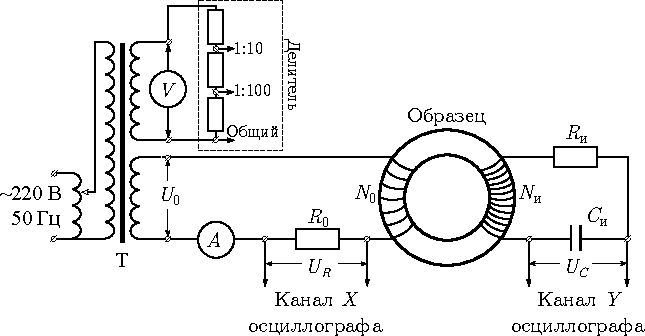
\includegraphics[width=\textwidth]{Chapter_4/4-5-exp.pdf}
    \caption{Схема установки для исследования намагничивания образцов}
    \figmark{experimental environment}
\end{figure}

В~цепь намагничивающей катушки, на которую подаётся некоторое напряжение
$U_0$, последовательно включено сопротивление $R_0$.
Напряжение на $R_0$, равное $U_R=R_0I_0$, где $I_0$ --- ток в
намагничивающей обмотке~$N_0$, подаётся на канал~$X$ осциллографа.
Связь напряжённости~$H$ в образце и тока~$I_0$ рассчитывается по теореме
о циркуляции (см.~\chaptereqref{H-toroid}).
\important{Действующее} значение переменного тока в обмотке~$N_0$ 
измеряется амперметром~$A$.

Для измерения магнитной индукции~$B$ с измерительной обмотки~$N_{и}$ на
вход $RC$-цепочки подаётся напряжение $U_{и}$ ($U_{вх}$),
пропорциональное производной~$dB/dt$.
С~интегрирующей ёмкости~$C_{и}$ снимается напряжение~$U_C$ ($U_{вых}$),
пропорциональное величине~$B$, и подаётся на вход~$Y$ осциллографа.
Значение индукции поля~$B$ рассчитывается по формуле~\eqref{4.5.4}.


Замкнутая кривая, возникающая на экране, воспроизводит в некотором масштабе
(различном для осей $X$ и $Y$) петлю гистерезиса. Чтобы придать этой кривой
количественный смысл, необходимо установить масштабы изображения, т. е. провести
калибровку каналов~$X$ и~$Y$ осциллографа.
% Для этого, во-первых, надо узнать,
% каким напряжениям (или токам) соответствуют амплитуды сигналов, видимых на экране, и,
% во-вторых, каким значениям~$B$ и~$H$ соответствуют эти напряжения (или токи).
%
% Значения напряжённости поля~$H$ пропорционально току~$I_0$ в намагничивающей
% катушке $N_0$ (а значит напряжению~$U_R=I_0 R_0$ на резисторе $R_0$)
% и рассчитывается по теореме о циркуляции (см.~\chaptereqref{H-toroid}).



% Напряжение, пропорциональное току в намагничивающей обмотке, подаётся на
% горизонтальную ось $X$.
% Если ручка усиления оси $X$ в положении калибр, цену
% деления по горизонтальной оси получим, разделив цену деления в вольтах
% на сопротивление $R_0$ в амперах.

% Для дополнительной проверки с помощью амперметра нужно закоротить обмотку $N_0$.

\paragraph{Калибровка осциллографа}
Калибровка канала~$X$ осциллографа производится с помощью амперметра $A$.
Предварительно необходимо закоротить обмотку $N_0$
(так как катушка с ферромагнитным образцом является
нелинейным элементом, ток в ней не имеет синусоидальной формы,
поэтому связать амплитуду тока с показаниями амперметра можно лишь
с довольно большой погрешностью). При закороченной обмотке~$N_0$
показания эффективного тока, умноженные на $2\sqrt{2}$,
дадут значение удвоенной амплитуды тока, подаваемого на ось $X$,
соответствующего ширине горизонтальной развёртки на экране
(осциллограф должен работать в режиме $X$--$Y$).

Калибровка вертикальной оси~$Y$, как правило, не нужна
(переключатель масштабов осциллографа откалиброван при изготовлении ---
при условии, что ручка плавной регулировки находится в положении
калибровки). Тем не менее, она может проводиться с помощью сигнала,
снимаемого через делитель напряжения со второй катушки понижающего трансформатора
(рис.~\figref{experimental environment}). Вольтметр $V$ может достаточно точно
измерить эффективное напряжение, подаваемое на вход осциллографа. После
этого можно сравнить показания осциллографа и вольтметра.

\paragraph{Измерение параметров интегрирующей ячейки}
Постоянную времени $RC$-цепочки можно определить экспериментально.
С~обмотки $U_0$ на вход интегрирующей цепочки подаётся синусоидальное напряжение
с частотой цепи $\nu_0=\frac{\omega_0}{2\pi}=50\;Гц$.
На вход~$Y$ осциллографа или цифрового вольтметра поочерёдно
подаются сигналы со входа ($U_\text{вх}=U_0$) и выхода ($U_\text{вых} = U_C$)
$RC$-цепочки. Измерив амплитуды этих сигналов, можно рассчитать постоянную
времени $\tau_{и}= R_{и}C_{и}$ по формуле \eqref{4.5.5}.
Кроме того, сопротивление и ёмкость можно независимым образом измерить
цифровым мультиметром.
% \begin{equation}
% 	\eqmark{4.5.6}
% 	RC = \frac{U_\text{вх}}{\omega U_\text{вых}}
% \end{equation}

\begin{lab:task}

\taskpreamble{В~работе предлагается при помощи электронного осциллографа
исследовать предельные петли гистерезиса и
начальные кривые намагничивания для нескольких ферромагнитных образцов;
определить магнитные характеристики материалов, чувствительность каналов $X$ и
$Y$ осциллографа и постоянную времени $\tau$ интегрирующей цепочки.}

\tasksection{Измерение петли гистерезиса}

\item
Для наблюдения петли гистерезиса на экране электронного осциллографа~(ЭО)
соберите схему рис.~\figref{experimental environment}. 
Подготовьте приборы к работе согласно техническому описанию в лаборатории.

\item \label{p45-1}
Подберите ток питания в намагничивающей обмотке, так чтобы на экране ЭО
наблюдалась \emph{предельная} петля гистерезиса. При этом 
при изменении тока в намагничивающей катушке 
у петли меняется длина <<усов>>~CD 
и~C$'$D$'$ (см. рис.~\figref{loop}), а её площадь остаётся
практически неизменной.

\item Подберите коэффициенты усиления каналов осциллографа так, 
чтобы предельная петля занимала б\'{о}льшую часть экрана.
Зафиксируйте (сфотографируйте или зарисуйте на кальку)
наблюдаемую картину.

Запишите значения коэффициентов усиления~$K_x$ и~$K_y$ осциллографа 
(убедитесь, что ручки плавной регулировки масштабов находятся
в калиброванном положении!) и действующее значение тока~$I$ 
в намагничивающей обмотке (по амперметру $A$).

\item \label{p45-2} По экрану ЭО~измерьте полную ширину и высоту
предельной петли ($[2X_{s}]$ и $[2Y_{s}]$),
соответствующие удвоенной амплитуде колебания 
напряжённости $H_s$ и индукции $B_s$ поля в образце в состоянии насыщения.

\item \label{p45-3} По экрану ЭО~измерьте двойные амплитуды 
для коэрцитивного поля $[2X_c]$ (ширина петли на пересечении с осью абсцисс) и
остаточной индукции $[2Y_r]$ (высота петли на пересечении с осью ординат).

При необходимости изменяйте коэффициенты усиления~$K_x$ и~$K_y$,
записывая их значения.

\item 
Проведите измерение начальной кривой намагничивания. 
Для этого плавно уменьшая амплитуду тока
намагничивания до нуля (8--10 точек), фиксируйте
по экрану осциллографа положения крайних точек наблюдаемых частных петель
(т.~А~и A$'$ на рис.~\figref{loop}).
Эти вершины лежат на начальной кривой намагничи­вания.
При необходимости фиксируйте (фотографируйте/отмечайте на кальке)
вид получаемых частных петель.

\item \label{p45-6} Запишите материал образца и параметры тороида.

\item Повторите измерения пп.~\ref{p45-1}--\ref{p45-6} 
для остальных катушек.

\tasksection{Калибровка осциллографа}

\item \label{p45-8}
Проведите калибровку горизонтальной оси осциллографа. 
Для этого не разбирая схемы рис.~\figref{experimental environment} 
<<закоротите>> намагничивающую обмотку~$N_0$ 
(подключите соединительные провода к одной клемме). 

Измерьте длину наблюдаемой развертки по оси~$X$ при некотором фиксированном 
токе~$I$, близком к току насыщения петли гистерезиса 
(осциллограф в режиме $X$--$Y$). 
Проведите измерения для всех значений коэффициента усиления~$K_x$, 
использовавшихся в работе. 
Учтите, что амперметр измеряет действующее значение тока, 
меньшее амплитудного в  $\sqrt{2}$ раз.

\item
Для проверки калибровки вертикальной оси ЭО~подключите вольтметр и осциллограф 
к делителю 1:100 (рис.~\figref{experimental environment}) и сравните показания
вольтметра и осциллографа. Оцените погрешность измерений амплитуды
с помощью осциллографа.

\tasksection{Определение параметров $RC$-ячейки}

\item
Измерьте постоянную времени $RC$-ячейки $\tau_{и}$ (см.~\eqref{4.5.5}). 
Для этого разберите цепь тороида и подайте на вход ячейки
(см. рис.~\figref{integrating curcuit}) синусоидальное напряжение 
с обмотки~$U_0$ понижающего трансформатора.

\item Измерьте отношение входного и выходного напряжений 
$U_\text{вх} / U_\text{вых}$ ячейки с помощью осциллографа и/или вольтметра.
Рассчитайте постоянную времени по формуле \eqref{4.5.5}.
Частоту сигнала в цепи $\omega_0=2\pi\nu_0$ 
можно также измерить с помощью осциллографа.


\item Сравните результат с расчётом непосредственно 
через~$R_\text{и}$ и~$C_\text{и}$, указанные на установке
(или измеренные с помощью мультиметра).


\tasksection{Обработка результатов}

% \item
% Сравните экспериментальное значение $\tau$ с расчётом через параметры
% $R_\text{и}$ и $C_\text{и}$, указанные на установке.

\item Рассчитайте коэффициенты преобразования отклонений по осям
$X$--$Y$ осциллографа в напряжённость~$H$ и индукцию~$B$ магнитного поля
в образце.

При расчётах используйте связь напряжённости и тока в тороидальном образце
(см. п. \ref{sec:toroid-measure} Введения), результаты п.~\ref{p45-8} 
калибровки канала~$X$, а также формулу \eqref{4.5.4}.

\item 
По результатам п.~\ref{p45-2} для каждого образца рассчитайте 
амплитуду $H_{\rm max}$ колебаний напряжённости поля в тороиде, 
соответствующую состоянию насыщения (предельная петля).
Вычислите индукцию насыщения образца~$B_s$.

\item По результатам п.~\ref{p45-3} для каждого образца
рассчитайте коэрцитивное поле~$H_c$ и остаточную индукцию~$B_r$.

\item Постройте начальные кривые намагничивания в координатах $B(H)$.
По графикам оцените начальное и максимальное значения дифферецниальной
магнитной проницаемости $\mu_\text{диф}=dB/dH$.

\item Оцените погрешности результатов эксперимента 
и сравните их с табличными.
% . Сведите результаты в таблицу:
% \begin{center}
% \begin{tabular}{|c|c|c|c|}
% \hline
% $\text{Ампл.}$ & $Fe-Ni$ & $Fe-Si$ & $\text{Феррит}$ \\
% \hline
% $H_c, \frac{\text{А}}{\text{м}}$ & $\frac{\text{эксп.}}{\text{табл.}}$ & & \\
% $B_s, \text{Тл}$ & & & \\
% $\mu_\text{диф}$ & & & \\
% \hline
% \end{tabular}
% \end{center}
\end{lab:task}

\begin{lab:questions}

\item Как в работе измеряются напряжённость~$H$ и индукция магнитного поля~$B$?

\item
При какой форме образцов, помещённых в однородное магнитное поле, их
намагниченность постоянна по всему объёму?

\item
Почему для наблюдения петли гистерезиса используются образцы в форме тора,
а не стержня?

\item
Почему при калибровке горизонтальной оси осциллографа необходимо от­ключать
намагничивающую обмотку?

\item
Оцените погрешность, которая возникает при измерении индукции $B$, если
измерительная катушка неплотно надета на образец; например, если образец
занимает всего половину охватываемой ею площади.

\item
Оцените погрешность, которая возникает из-за конечной глубины проникновения
переменного магнитного поля в образец.

\item Предложите альтернативные способы интегрирования сигнала в цепи.

\end{lab:questions}


\begin{lab:literature}
\item \Kirichenko~--- \S~4.1, 4.2, 9.3.

\item \SivuhinIII~--- \S\S~74, 79.

\item \Kalashnikov~--- \S\S~110, 111, 119.

\item \KingLokOlh~--- Ч. II, гл. 5, \S~5.3.
\end{lab:literature}

\lab{Параметрический резонанс в контуре с нелинейной индуктивностью}

\aim{изучение параметрических колебаний в электрической цепи.}

\equip{параметрон (две тороидальных катушки, резисторы, интегрирующая цепочка,
конденсаторы), генератор звуковых частот, реостат, сглаживающий дроссель,
магазин ёмкостей, магазин сопротивлений, вольтметр, миллиамперметр,
осциллограф.}

Перед выполнением работы рекомендуется ознакомиться с
пп.~\ref{sec:ferromagnetism}--\ref{sec:forces} теоретического
введения к разделу.

Если периодически изменять ёмкость конденсатора или самоиндукцию катушки,
входящих в состав колебательного контура, то при определённых условиях в контуре
возбуждаются незатухающие электрические колебания. Такой способ возбуждения
называется \term{параметрическим,} поскольку колебания возникают не под
действием внешней ЭДС, а вследствие изменения параметров контура.

Рассмотрим колебательный контур, состоящий из последовательно соединённых
ёмкости $C$, индуктивности $L$ и сопротивления $R$. В силу неизбежных внешних
влияний и тепловых флуктуаций в контуре всегда имеют место небольшие колебания с
частотой $\omega_0$, которая при малых потерях зависит только от реактивных
параметров $L$ и $C$:
\begin{equation}
	\eqmark{4.6.1}
	 \omega_0 = \frac{1}{\sqrt{LC}}.
\end{equation}

При этом средняя полная энергия $W$, запасённая в контуре, остаётся постоянной;
происходит лишь её периодическая перекачка с частотой $2\omega_0$ из
электрической $W_\text{Э} = q^2 / (2C)$ в магнитную $W_M = LI^2/2$ и обратно.
Здесь $q$~--- заряд на обкладках конденсатора, $I$~--- ток в катушке
индуктивности. Полную энергию системы можно изменить, если скачком поменять
величину $L$ (или $C$).

 Рассмотрим, как изменяется энергия контура при быстром уменьшении $L$
(например, растяжении катушки) в тот момент, когда ток в катушке максимален.
Сумма падений напряжения на элементах контура равна ЭДС самоиндукции:
\begin{equation*}
	RI + \frac{q}{C}= - \frac{d(LI)}{dt}
\end{equation*}

Проинтегрируем это уравнение по времени за очень короткий промежуток $\Delta t
~(\Delta t \ll 1/\omega_0)$ в течение которого изменяется индуктивность. Два
первых интеграла при этом будут близки к нулю, поэтому можно считать, что
магнитный поток $\Phi$ в катушке в течение этого времени не изменяется:
$\Delta \Phi=\Delta (LI) = 0$ или
\begin{equation}
	\eqmark{4.6.2}
	\Phi=LI =\const.
\end{equation}

Уменьшение индуктивности в тот момент, когда ток в контуре максимален, ведёт к
увеличению тока и магнитной энергии в катушке:
\begin{equation*}
	\Delta W_M = \Delta \left(\frac{\Phi^2}{2L}\right) = - (LI)^2\frac{\Delta
L}{2L^2} = - \frac{I^2}{2}\Delta L
\end{equation*}

Если теперь через четверть периода вернуть индуктивность к прежнему значению~---
энергия системы не изменится, так как ток в этот момент равен нулю. Ещё через
четверть периода опять уменьшим $L$~--- снова возрастёт энергия. Процесс
увеличения энергии системы за счёт работы внешних сил называют накачкой.
Заметим, что индуктивность при этом меняется с частотой, вдвое превосходящей
собственную частоту контура.

Энергия, которую получает контур за период $T$:
\begin{equation*}
	2W_M = I^2_{max} \Delta L,
\end{equation*}
должна превышать потери на активном сопротивлении, составляющие
\begin{equation*}
	W_R = RI^2_\text{эфф}T.
\end{equation*}

При выполнении условия $2W_M > W_R$ или $\Delta L > RT/2$ амплитуда колебаний в
контуре возрастает с каждым периодом. С увеличением амплитуды всё более
возрастает роль нелинейной зависимости $B(H)$, что ограничивает возрастание
амплитуды. Поэтому со временем в контуре устанавливаются колебания максимально
возможной постоянной амплитуды. Это явление называют \term{параметрическим
резонансом.}

То, что амплитуда установившихся колебаний определяется именно нелинейностью, а
не потерями, является принципиальным отличием параметрических колебаний от
обычного резонанса.

Раскачка колебаний возможна при изменении $C$ или $L$ по любому периодическому
закону с частотами $\Omega_\text{Н}$, для которых справедливо соотношение
\begin{equation*}
	\frac{\omega_0}{\Omega_\text{Н}} = \frac{n}{2},
\end{equation*}
где $n$ --- целое число (1,~2,~$\dots$). Наиболее эффективная раскачка имеет
место при $n$ = 1, когда частота накачки $(\Omega_\text{Н})$ равна частоте
колебаний энергии $W_\text{Э}$ и $W_M~(2\omega_0).$

 В том случае, когда индуктивность изменяется по синусоидальному закону, условие
возбуждения колебаний имеет вид
\begin{equation}
	\eqmark{4.6.3}
	\Delta L > \frac{2RT}{\pi}.
\end{equation}
Величиной индуктивности можно управлять током подмагничивания.

\begin{figure}[h!]
    \centering
    \pic{0.5\textwidth}{Chapter_4/4_6_1}
    \caption{Полная и частная петли гистерезиса}
    \figmark{hysteresis loop}
\end{figure}

На рис.~\figref{hysteresis loop} показана зависимость~$B(H)$ в ферромагнитном
сердечнике~--- петля гистерезиса. Меняя поле~$H$ можно выбрать такую рабочую
точку на петле, вблизи которой зависимость~$B(H)$ обладает наиболее ярко
выраженной нелинейностью. На рис.~\figref{hysteresis loop} это точка $A$:
вблизи неё особенно резко изменяется дифференциальная магнитная
проницаемость $\mu_\text{диф}$ (производная
$d\mu_\text{диф}/dH$ максимальна).

Соответствующее подмагничивающее поле $H_\text{п}$ задаётся постоянным током,
проходящим через дополнительную (подмагничивающую) обмотку.

Небольшие колебания величины~$B$ вокруг рабочей точки можно создать, подав на
вторую подмагничивающую обмотку переменный ток подмагничивания. Магнитная
проницаемость $\mu_\text{диф}$, а с ней индуктивность $L$, будут меняться с той
же частотой, что и переменная составляющая подмагничивающего тока (из-за
нелинейности $B(H)$ в кривой $\mu(t)$ присутствуют также колебания с кратными
частотами, не представляющие для нас интереса). Если изменения индуктивности
достаточно велики, то в контуре возбуждаются незатухающие колебания, частота
которых вдвое меньше частоты изменения параметров контура (в нашем случае~---
частоты изменения индуктивности, то есть частоты подмагничивания). Такое
соотношение частот служит отличительным признаком параметрических колебаний.

\experiment
Для изучения параметрических колебаний используется <<параметрон>>~--- установка
с нелинейной индуктивностью, схема которой представлена на
рис.~\figref{experimental environment}. <<Параметрон>> включает в себя две
тороидальных катушки, интегрирующую ячейку $r_0C_0$ (см. описание
принципа работы интегрирующей ячейки в работе \ref{lab:4-5}),
резисторы $r_1$ и~$r_2$, ключи~$K_1$ и~$K_2$ и колебательный контур.
Колебательный контур состоит из двух последовательно соединённых
индуктивностей~$L_1$ и~$L_2$, ёмкости~$C$ и сопротивлений~$R_M$ и~$r_2$.
На рисунке контур заключён в пунктирную рамку.
\begin{figure}[h!]
\centering
	\pic{\textwidth}{Chapter_4/4_6_2}
	\caption{Схема установки}
	\figmark{experimental environment}
\end{figure}

Обе катушки $L_1$ и $L_2$ с одинаковым числом витков~$n_1$ намотаны на
одинаковые тороидальные ферромагнитные сердечники. Длина каждого сердечника~---
$l$, сечение~--- $S$, магнитная проницаемость~--- $\mu$. 
С~помощью теоремы о циркуляции можно показать, что общая индуктивность катушек
\begin{equation}
	\eqmark{4.6.5}
	L = 2\mu_0\mu\frac{n^2_1S}{l}
\end{equation}

Постоянный ток подмагничивания от источника постоянного напряжения 36~В проходит
через две последовательно соединённые обмотки с числом витков~$n_2$. Ток
регулируется потенциометром~$\text{П}$. Для того, чтобы увеличить сопротивление
цепи переменному току, поставлена индуктивность $L_0 = 3~$Гн. Переменный ток в
этой цепи практически отсутствует, постоянный измеряется амперметром~$A$.

Переменный ток подмагничивания, создаваемый генератором звуковых частот,
проходит через последовательно соединённые обмотки~$n_3$. Обмотка~$n_4$ имеется
всего на одном из сердечников. Она служит для измерения полного магнитного
потока, проходящего через сердечник. Обмотки $n_1$ соединены так, что
возникающие в них ЭДС имеют противоположые знаки, поэтому в колебательном
контуре не возникают токи, имеющие частоту звукового генератора.

Для измерения напряжений в схему включён вольтметр переменного тока. При
переключении ключа $K_2$ в верхнее положение вольтметр измеряет напряжение
$U_\text{ЗГ}$ на выходе генератора, при переключении в нижнее --- выходное
напряжение на ёмкости $C$. Осциллограф позволяет наблюдать петлю гистерезиса,
фиксировать момент возникновения и срыва параметрических колебаний и определять
их частоту с помощью фигур Лиссажу.

При верхнем положении ключа $K_1$ на вход $X$ осциллографа подаётся падение
напряжения между точками 1 и 7, практически равное напряжению $U_{\text{ЗГ}}$ на
генераторе (падением напряжения на резисторах $r_1$, $r_2$ можно пренебречь,
поскольку оно мало по сравнению с $U_{\text{ЗГ}}$). На вход $Y$ подаётся
напряжение с ёмкости $C$ колебательного контура. По фигурам Лиссажу, возникающим
на экране, можно сравнить частоту накачки (частоту генератора) с частотой
колебаний контура.

При нижнем положении ключа $K_1$ на вход $Y$ подаётся напряжение $U_Y$ с ёмкости
$C_0$. Эта ёмкость входит в состав интегрирующей цепочки $r_0C_0$, подключённой
к обмотке $n_4$. ЭДС индукции, возникающая в обмотке $n_4$, пропорциональна
$dB/dt$:
\begin{equation*}
	U_4 = n_4S\frac{dB}{dt}.
\end{equation*}

Параметры интегрирующей цепочки подобраны так, что сопротивление $r_0$ заметно
превышает сопротивление обмотки $n_4$ и сопротивление ёмкости:
\begin{equation*}
	r_0 \gg \frac{1}{\omega_0C_0}.
\end{equation*}

 При этом условии ток в цепочке пропорционален $dB/dt$:
\begin{equation*}
	I_0 = \frac{U_4}{r_0} = \frac{n_4S}{r_0}\frac{dB}{dt},
\end{equation*}
а напряжение $U_Y$ на конденсаторе $C_0$ пропорционально $B$:
\begin{equation}
	\eqmark{4.6.6}
	U_Y = \frac{1}{C_0}\int I_0dt = \frac{1}{r_0C_0}\int U_4dt =
\frac{n_4S}{r_0C_0}B.
\end{equation}

На вход $X$ осциллографа подаётся сумма падений напряжения на резисторах $r_1$ и
$r_2$. Напряжение, возникающее на $r_1$, пропорционально току, протекающему
через обмотки $n_3$ от генератора. В отсутствие параметрических колебаний через
$r_2$ ток не течёт, и на вход $X$ подаётся напряжение $U_X$, пропорциональное
переменному току подмагничивания $I$, которым определяется поле $H$ в
сердечнике:
\begin{equation*}
	H = \frac{n_3I}{l}.
\end{equation*}
Следовательно,
\begin{equation}
	\eqmark{4.6.7}
	U_X = Ir_1 = \frac{lr_1}{n_3}H.
\end{equation}

Таким образом, в отсутствие параметрических колебаний на экране появляется
кривая гистерезиса ферромагнитного сердечника. При возникновении колебаний в
контуре через $r_2$ начинает проходить ток, кривая резко искажается и для
измерений непригодна. Но искажение петли позволяет отметить момент возникновения
параметрических колебаний и даёт возможность измерить параметры петли при
подходе к моменту самовозбуждения. Сфотографировав или зарисовав с экрана на кальку петлю
гистерезиса, соответствующую границе возбуждения параметрических колебаний,
можно экспериментально проверить справедливость формулы \eqref{4.6.3}~---
условия самовозбуждения. Из \eqref{4.6.5} следует
\begin{equation}
	\eqmark{4.6.8}
		\Delta L = L_{\rm max} - L_{\rm min} =
        \frac{2\mu_0n^2_1S}{l}\left(\mu_{\rm max} - \mu_{\rm min}\right)
		= \frac{2n^2_1S}{l}
%         \left[\left(\frac{dB}{dH}\right)_{max} -
        \left.\frac{dB}{dH}\right|_{\rm min}^{\rm max},
\end{equation}

Производные $dB/dH$ следует взять из чертежа, проведя касательные к кривой
$B(H)$ слева и справа от излома петли. Для расчёта масштабов выразим $B$ и $H$
через напряжения $U_Y$ и $U_X$. Подставляя \eqref{4.6.6} и \eqref{4.6.7} в
\eqref{4.6.8}, получим
\begin{equation}
	\eqmark{4.6.9}
	\Delta L = 2r_0C_0r_1\frac{n^2_1}{n_3n_4}\left[\left(\frac{\Delta
U_Y}{\Delta U_X}\right)_{\rm max} - \left(\frac{\Delta U_Y}{\Delta
U_X}\right)_{\rm min}\right].
\end{equation}
В нашей установке $n_3 = n_4$, так что $n_1^2/ (n_3n_4) = 1$. Параметры $r_0$,
$C_0$ приведены на установке.

\begin{lab:task}

\taskpreamble{В работе предлагается с помощью фигур Лиссажу найти критическое сопротивление и
определить частоту параметрических колебаний контура; с помощью кривых
гистерезиса определить критическое сопротивление и проверить условие
самовозбуждения; по кривой зависимости напряжения на конденсаторе от частоты
определить резонансную частоту и индуктивность колебательного контура.}

\item
Соберите схему согласно рис.~\figref{parametron}. Сравните схему, изображённую
на рис.~\figref{parametron}, со схемой на рис.~\figref{experimental
environment}. Подготовьте приборы к работе.
\begin{figure}[h!]
\centering
	\pic{\textwidth}{Chapter_4/4_6_3}
	\caption{Блок-схема установки}
	\figmark{parametron}
\end{figure}

\item
Установите ёмкость $C = 100$~мкФ, сопротивление магазина $R_M =~0.$ Поставьте на
минимум выходного напряжения движок потенциометра, регулирующего постоянный ток
подмагничивания. Включите питание $= 36$~В и установите постоянный ток $I
=80$~мА. Переменный ток подмагничивания установите с помощью генератора: частота
$\nu = 150$~Гц; выходное напряжение на вольтметре генератора $U_\text{ЗГ} =
15$~В.

\item
\begin{minipage}[t]{0.6\textwidth}
Для наблюдения параметрических колебаний поставьте ключ $K_1$ в положение
<<Фигура Лиссажу>>. Увеличивая постоянный ток подмагничивания, определите момент
возникновения параметрических колебаний (при $U_\text{ЗГ} = 15$~В) по появлению
на экране ЭО фигуры Лиссажу, имеющей одно самопересечение (рис.~\figref{figures
of lissage}a). Оцените интервал $\Delta I$, внутри которого эти колебания
существуют. Используя показания генератора, определите по виду фигуры Лиссажу
частоту параметрических колебаний.
\end{minipage}
\hfil
\begin{minipage}[t]{0.3\textwidth}
%\begin{figure}[h!]
\vspace*{1pt}
\centering
	\pic{\linewidth}{Chapter_4/4_6_4}
	\captionof{figure}{%
       Фигуры Лиссажу при отношении частот~1:2 (масштабы разные).
       \figmark{figures of lissage}}
%\end{figure}
\end{minipage}

\item
Убедитесь в том, что Вы наблюдаете именно параметрические колебания, внеся в
контур дополнительное затухание~--- увеличивая сопротивление магазина $R_M$.
Колебания, возбуждаемые внешним источником, при увеличении затухания постепенно
уменьшаются по амплитуде, в то время как параметрические колебания при
критическом сопротивлении $R_\text{кр}$ срываются.

\item
Определите $R_\text{кр}$ для токов: $I = 100$~мА и $I = 160$~мА. Увеличивая
сопротивление магазина, следите за постоянством напряжения на генераторе
($U_\text{ЗГ} = 15$~В).

\item
При фиксированных значениях: $I = 160$~мА, $U_\text{ЗГ} = 15$~В, $R_M = 0$~---
проследите, как изменяется фигура Лиссажу при уменьшении частоты от 150 до
50~Гц. Определите резонансную частоту и частоту срыва колебаний.

\item
Для наблюдения петли гистерезиса переключите ключ $K_1$ в положение «Петля».
Снова задайте параметры: $I = 160$~мА, $R_M = 0$, $\nu = 150$~Гц, $U_\text{ЗГ} =
15$~В. Подберите чувствительность осциллографа так, чтобы на экране была видна
петля гистерезиса в удобном масштабе.

При наличии параметрических колебаний петля гистерезиса имеет сложную форму.
Увеличьте сопротивление $R_M$ до критического. В этом случае параметрические
колебания срываются и на экране видна частная петля (на рис.~\figref{hysteresis
loop} она выделена пунктиром).

Чтобы увидеть форму полной петли, уберите сопротивление $R_M$ и ток $I$ до нуля.
При увеличении напряжения $U_\text{ЗГ}$ до 20~--~25~В полная петля становится
предельной.

\item
Увеличивая постоянный ток, проследите, как меняется форма петли в момент
возникновения и срыва параметрических колебаний, как перемещается частная петля.

\item
Для тока $I = 160$~мА, $U_\text{ЗГ} = 15$~В определите $R_\text{кр}$, выводя
параметры на самую границу колебаний.

\item
При сопротивлении чуть больше критического сфотографируйте или зарисуйте петлю.
Для этого установите
ручки плавной регулировки усиления по каналам $X$ и $Y$ в крайнее правое
положение (до щелчка), тогда цифры возле дискретных переключателей усиления
задают масштабы изображения $K_X$ и $K_Y$ в~мВ/дел.

Подберите коэффициенты усиления так, чтобы петля занимала практически весь
экран. Зарисуйте на кальку петлю, оси координат, деления шкалы и запишите на ней
рабочие параметры схемы и коэффициенты $K_X$ и $K_Y$.

\item Исследуйте зависимость выходного напряжения параметрона от частоты. Для
этого уменьшите сопротивление магазина до нуля и поставьте ключ $K_2$ в
положение <<$U_\text{вых}$>>. Снимите зависимость напряжения на ёмкости $C$
колебательного контура $U_\text{вых} = f(\nu)$, уменьшая частоту от 150~Гц до
срыва колебаний. Напряжение $U_\text{ЗГ} = 15$~В и ток $I = 160$~мА следует
поддерживать постоянными.

\tasksection{Обработка результатов}

\item
Определите по рисунку петли максимальный и минимальный наклоны касательных
$(\Delta U_Y/ \Delta U_X)$ и рассчитайте величину $\Delta L$ по формуле
\eqref{4.6.9}.

Проверьте справедливость условия \eqref{4.6.3}. Полное сопротивление контура
включает в себя сопротивление магазина и сопротивление параметрона между точками
5 и 7, указанное на установке.

\item
Постройте график $U_\text{вых} = f(\nu)$ и определите по нему резонансную
частоту контура $\nu_0$. Рассчитайте индуктивность контура
и проверьте справедливость условия \eqref{4.6.3} на
этой частоте, полагая $\Delta L \sim L$.

\end{lab:task}


\begin{lab:questions}
\item
Получите условие возбуждения колебаний \eqref{4.6.3}, когда индуктивность
меняется по гармоническому закону: $L = L_0(1-m\sin(2\omega_0t))$. Напишите закон
изменения тока, возбуждаемого в контуре.

\item
Почему в нашем случае индуктивность пропорциональна дифференциальной магнитной
проницаемости?

\item
Нарисуйте качественный график зависимости $\mu_\text{диф}$ от величины
подмагничивающего тока для петли гистерезиса, которая изображена на
рис.~\figref{hysteresis loop}.

\item
На каких ещё частотах (в принципе) могут возбуждаться колебания в контуре
параметрона при больших изменениях индуктивности?
\end{lab:questions}


\begin{lab:literature}
\item
\SivuhinIII~--- Гл. III, \S 74; гл. X, \S\S~122, 123, 127, 135.

\item
\Kalashnikov~--- \S~226.

\item
\KingLokOlh~--- Ч. III, гл. 3, 3.1.

\item
\textit{Горелик~Г.С.} Колебания и волны. --- М.:~Физматгиз, 1959. Гл. III, \S~9.

\end{lab:literature}


\cleardoublepage
\chapter{Плазма. Газовый разряд}

\introsection{Введение}

Как известно, вещество может находиться в трёх агрегатных состояниях~--- твёрдом,
жидком и газообразном, причём эти
состояния последовательно сменяются по мере возрастания температуры. Если~и
дальше нагревать газ, то сначала молекулы диссоциируют на атомы, а~затем и атомы
распадаются на электроны и ионы, так что газ становится \emph{ионизованным},
представляя собой смесь из свободных электронов и ионов, а~также нейтральных
частиц. Если \emph{степень ионизации} газа
(отношение числа ионизованных атомов к их полному числу) оказывается достаточно велика, то
такой газ может обладать качественно новыми свойствами.
Поведение заряженных частиц приобретает \emph{коллективный} характер, 
так что описание свойств среды не может быть 
сведено к обычному газу, содержащему некоторое количество отдельных заряженных частиц.
Такое состояние ионизованного газа называется \term{плазмой}.
Плазму называют также четвёртым состоянием вещества.
Более точное количественное определение этого понятия будет дано ниже.

Из характерных свойств плазмы можно выделить высокую электропроводность и
\term{квазинейтральность}. Ввиду наличия большого числа подвижных
заряженных частиц плазма, в противоположность нейтральному газу, сильно
взаимодействует с электрическим и магнитным полями.
При этом частицы в плазме стремятся распределиться в пространстве таким образом,
чтобы средняя плотность заряда была равна нулю. Равенство концентраций
положительных и отрицательных частиц нарушается, как правило,
лишь в микроскопических масштабах из-за тепловых флуктуаций.

Первое описание газовой плазмы дал И.~Ленгмюр (1923~г.), исследуя электрический
разряд в газе низкого давления (\emph{тлеющий разряд}). Он назвал плазмой <<ярко
светящийся газ, состоящий из электронов, ионов разных сортов и нейтральных
атомов и молекул>>. Он же ввёл сам термин~--- плазма 
(от греческого глагола, обозначающего <<разрыхляться>>, <<расползаться>>).

Свечение плазмы, являющееся при относительно невысоких температурах 
следствием непрерывно идущей рекомбинации электронов и ионов в нейтральные атомы, 
сопровождается выделением энергии и уменьшением концентрации электронов и ионов. 
Стационарное состояние плазмы может существовать лишь при наличии непрерывно 
действующего источника энергии. Им может быть электрический разряд в газе 
(газоразрядная плазма),
происходящий в постоянном электрическом поле (обычный газовый разряд,
дуга и т.~д.) или в высокочастотном поле (индукционные катушки,
запитанные током высокой частоты электроды и т.~д.).
Плазма может образовываться и при \emph{термической} ионизации газа, 
если газовая среда поддерживается при достаточно высокой температуре 
(пламя газовой горелки). Плазма образуется в фокальной области мощных лазерных 
установок и при многих других условиях. 
Звёздная плазма существует за счёт выделения энергии в реакциях 
\emph{ядерного синтеза}.

Практическое применение плазмы чрезвычайно многообразно.
Например, низкотемпературная плазмы применяется 
для проведения химических реакций, которые в горячей
сильно ионизованной газовой среде происходят очень быстро и эффективно.
Методы плазменного травления применяются при создании интегральных
микросхем. Плазма исследуется также в связи с проблемой 
создания магнитогидродинамических генераторов~--- преобразователей
механической энергии движущегося в магнитном поле проводящего газа в
электрическую энергию.
Большой интерес представляет плазма, существующая в атмосфере Земли и планет, а
также в космосе. Атмосферная плазма создаётся ультрафиолетовым излучением
Солнца. Электроны плазмы захватываются магнитным полем Земли (движутся вокруг и
вдоль силовых линий магнитного поля) и образуют радиационные пояса на
расстояниях тысяч километров от поверхности Земли. Широко известны также
плазменные проводящие слои Хевисайда, обеспечивающие дальнюю радиосвязь
на коротких волнах. 
Наконец, физика плазмы является неотъемлемой частью проблемы создания 
\emph{управляемого термоядерного синтеза} (УТС).


В \term{низкотемпературной} плазме ($T\lesssim 10^4$~К) степень ионизации 
атомов обычно невелика. Например, в тлеющем газовом разряде 
люминесцентной лампы коцентрация электронов составляет 
$n_e\sim 10^9\;\text{см}^{-3}$,
а концентрация нейтральных молекул $n_0\sim 10^{14}\;\text{см}^{-3}$.
Лишь внутри звёзд и в установках, используемых для исследования проблем 
УТС, где температуры достигают значений $T \sim 10^{6}\;К$ и более
(\term{высокотемпературная} плазма),
доля ионизованных атомов приближается к единице.

\begin{figure}[ht]
    \centering
    {\footnotesize
    \pic{\textwidth}{Chapter_5/v5_0}}
    \caption{Различные типы плазмы в лаборатории и природе. Температура
    указана в энергетических единицах ($1\;эВ\approx 11\,600\;К$)}
    \figmark{Types of plasma}
\end{figure}

Стационарное состояние плазмы зачастую является \term{неравновесным}.
При этом её компоненты плазмы (электроны и ионы), как
правило, имеют разную температуру: $T_e\ne T_i$. 
Такое оказывается возможным, поскольку 
электроны и ионы имеют существенно разные массы ($m_e \ll m_i$).
Поэтому при электрон-ионных столкновениях обмен энергией идёт гораздо медленнее,
чем при столкновениях частиц одного сорта (электрон-электронных и ион-ионных).
Например, в тлеющем газовом разряде обычно имеются 
<<горячие>> электроны и <<холодные>> ионы: $T_e \gg T_i$.
Это связано с тем, что в сильно разреженном газе электроны ускоряются 
внешним электрическим полем, почти не теряя энергии при соударениях 
с ионами и атомами газа или стенками сосуда, --- в результате электроны
нагреваются до высоких температур $T_e\sim 10^4\;К$.
Ионы же, напротив, быстро отдают полученную от поля и от электронов энергию 
нейтральным атомам газа и атомам стенок, поскольку массы их близки, 
--- поэтому их температура оказывается порядка комнатной, $T_i \sim 300\;К$.


Свойствами, характерными для газовой плазмы, обладают и некоторые другие среды,
называемые по этой причине \emph{плазмоподобными} средами, или просто <<плазмами>>.
В~качестве примеров можно назвать плазму металлов,
плазму электролитов, электронно-дырочную плазму полупроводников, 
нуклонную плазму атомного ядра и др.
На рис.~\figref{Types of plasma} на плоскости параметров
$T$\,--\,$n$ (температура плазмы~--- плотность числа частиц) 
представлены различные типы плазм, встречающихся как в лабораторных условиях,
так и в природе.

% Под температурой плазмы в каждом конкретном случае понимают температуру тех
% заряженных частиц, которые определяют плазменные свойства рассматриваемой среды:
% в большинстве случаев это электроны.

Основные свойства газовых разрядов подробно рассмотрены
в Приложении к разделу (см. стр.~\pageref{sec:discharge}).

\introsection{Основные характеристики плазмы}
\label{sec:plasma}

Определяющими свойствами плазмы являются \emph{коллективный} характер её движения
и \emph{квазинейтральность} (равенство нулю средней плотности заряда).
Рассмотрим простейший вид коллективных плазменных колебаний. Здесь и далее
в этом разделе будем использовать систему СГС, как это принято в физике плазмы.

\introsubsection{Плазменная частота}

\begin{wrapfigure}{o}{0.45\textwidth}
    \centering
    \pic{0.9\linewidth}{Chapter_5/v5_1}
    \caption{Плазменные колебания}
    \figmark{1}
\end{wrapfigure}

Выделим в нейтральной плазме некоторый объём в виде параллелепипеда
(см. рис.~\figref{1}).
Обозначим концентрацию электронов как $n_e$; ионы для простоты будем считать
однозарядными ($Z=1$), тогда их концентрация такая же, как у электронов: $n_i=n_e$.
Предположим, что все электроны сместились на расстояние $x$ относительно ионов.
Ионы как существенно более тяжёлые частицы можно считать неподвижными.
% (ионы занимают объём, изображённый сплошными, а электроны~--- пунктирными линиями).
В результате на боковых гранях параллелепипеда возникнут нескомпенсированные
поверхностные заряды с плотностью
\begin{equation*}
%     \eqmark{5.13}
    \sigma = \pm n_e e \Delta x.
\end{equation*}
Эти заряды --- как две пластины конденсатора --- создадут электрическое поле
\begin{equation*}
%     \eqmark{5.14}
    E=4\pi n_e e \Delta x.
\end{equation*}
В свою очередь это поле будет действовать на электроны,
придавая им ускорение, равное
\begin{equation*}
%     \eqmark{5.15}
    \frac{d^2\Delta x}{dt^2}=-\frac{eE}{m}=-\frac{4\pi ne^2}{m} \Delta x.
\end{equation*}
Видно, что полученное уравнение описывает гармонические колебания с частотой
\begin{equation}
    \eqmark{plasma-freq}
    \omega_p=\sqrt{\frac{4\pi n_e e^2}{m_e}}.
\end{equation}

Таким образом, мы получили частоту коллективных колебаний
электронов относительно квазинейтрального состояния. Такие колебания
называют \term{ленгмюровскими}, а частоту $\omega_p$ ---
\term{плазменной} или \term{ленгмюровской}. Эта частота ---
один из важнейших параметров плазмы.
Она определяет характерный \emph{временной} масштаб для плазмы --- время
отклика на флуктуацию плотности заряда в ней. Частота $\omega_p$
определяет многие физические процессы, включая распространение 
электромагнитных волн в плазме.

% Для рассчётов можно использовать практическую формулу
% \begin{equation}
%     \eqmark{omegap-practical}
%  \omega_p =5,65\cdot10^4\sqrt{n[\text{см}^{-3}]}\;рад/с.
% \end{equation}

\introsubsection{Дебаевский радиус}\label{sec:debye_rad}

Плазменные колебания могут быть возбуждены как с счёт внешнего воздействия
(например, при прохождении электромагнитной волны), так и за счёт
тепловой энергии, содержащейся непосредственно в плазме.
Оценим их амплитуду в последнем случае.

Средняя скорость, которую могут приобрести электроны за счёт тепловых
флуктуаций по порядку величины равна $\bar{v}_e\sim \sqrt{\kB T/m_e}$, 
где $T$~--- температура электронов. Амплитуду $r$ колебаний 
электронов относительно ионов можно оценить как смещение с тепловой 
скоростью $\bar{v}_e$ за характерное время колебаний $1/\omega_p$:
\begin{equation*}
r \sim \frac{\bar{v}_{e}}{\omega_p}=\sqrt{\frac{\kB T}{4\pi n_e e^2}}.
\end{equation*}

Полученную величину обозначают как
\begin{equation}
\eqmark{debye-rad}
r_D=\sqrt{\frac{\kB T}{4\pi n_e e^2}},
\end{equation}
и называют \term{дебаевским радиусом} 
(или \term{дебаевской длиной}). Это ещё один важный плазменный параметр, 
задающий характерный \emph{пространственный} масштаб многих плазменных явлений.

%Оценим амплитуду колебаний электронов относительно ионов,
%возникающих за счёт тепловых флуктуаций.
%Пусть облако электронов, рассмотренное в предыдущем пункте, 
%колеблется с некоторой амплитудой $x_0$ и частотой $\omega_p$.
%
%Как известно из теории колебаний, амплитуда скорости равна $v_0 = \omega_p x_0$,
%а полная энергия колебаний равна максимальному значению кинетической энергии.
%Тогда в расчёте на единицу объёма среды имеем энергию 
%$w= \frac12 n_e m_e (\omega_p x_0)^2$.
%С другой стороны, из термодинамики известно, что эта энергия должна
%быть равна тепловой энергии, приходящейся на одну степень свободы
%$W_{Т} = \frac12 \kB T_e$. Отсюда находим $x_0^2 = \frac{\kB T_e/m_e}{\omega_p^2}$.


Из рассмотренного примера видно, что дебаевская длина есть амплитуда ленгмюровских колебаний,
возбуждаемых тепловыми флуктуациями. Она задаёт масштаб, на котором возможно
спонтанное нарушение квазинейтральности плазмы.
%Заметим также, что формулу \eqref{debye-rad} можно переписать как
%где $v_{Te}=\sqrt{\kB T_e/m_e}$~--- скорость, по порядку величины равная
%средней тепловой скорости движения электронов.

Таким образом, плазменная частота $\omega_p$ и дебаевская длина $r_D$
есть две важнейшие характеристики плазмы, определяющие в том числе
временной и пространственный масштабы коллективного движения электронов
относительно ионов.

% Как следует из \eqref{plasma-freq}, плазменная частота определяется только плотностью
% электронов (и универсальными постоянными).
% Можно строго доказать, что она не зависит от формы рассматриваемого возмущения и
% является, таким образом,
% локальной характеристикой плазмы. Плазменная частота является не
% единственной~--- но важнейшей~--- характерной частотой
% плазмы. Она определяет коллективное движение электронов относительно ионов.

\introsubsection{Плазменное экранирование}

Рассмотрим ещё одну задачу, в которой дебаевская длина играет роль
ключевого параметра.

\begin{wrapfigure}{o}{0.3\textwidth}
    \centering
    \pic{\linewidth}{Chapter_5/v5-screen1}
    \caption{Упрощенная геометрия задачи об экранировании заряда}
\end{wrapfigure}

Поместим в равновесную плазму с температурой $T$ ($T_e=T_i$) некоторую пробную частицу, 
имеющую фиксированный
положительный $+q$ и найдём, как распределятся плазменные частицы вокруг неё.
Будем считать, что частица достаточно массивна, так что её можно
считать неподвижной (в качестве такого пробного заряда можно рассмотреть
один из ионов плазмы, поскольку $m_i \gg m_e$).

Заряд будет притягивать к себе плазменные электроны, в результате чего
вокруг него образуется отрицательно заряженное <<облако>>,
\emph{экранирующее} поле заряда на большом расстоянии от него ---
электрическое поле вокруг~$q$ будет убывать с расстоянием~$r$
не по закону $q/r^2$, а существенно быстрее.
Если бы электроны не имели кинетической энергии, то они так <<облепили>>
бы пробный заряд, что его собственное поле было бы полностью скомпенсировано.
Тепловое движение мешает такой компенсации.

Чтобы наглядно выявить характерные особенности решения данной задачи,
предположим, что радиус~$r_0$ пробной частицы велик (по сравнению с $r_D$)
и будем рассматривать распределение поля вблизи её поверхности ---
так мы сведём задачу к одномерной, сильно упростив выкладки, но не потеряв
качественные особенности решения.

Пространственное распределение электронов в равновесии подчиняется
\important{закону Больцмана}:
\begin{equation}
    \eqmark{5.5}
    n_e=n_{e0} \cdot \exp\left(\frac{e\varphi}{\kB T}\right)
\end{equation}
Здесь $\varphi$~--- потенциал электростатического поля,
$n_{e0}$ --- концентрация электронов вдали от заряда, где $\varphi\to 0$.
Аналогичное соотношение можно записать и для ионов с заменой $-e\to e$
(по-прежнему считаем, что $Z=1$).
% \begin{equation}
%     \eqmark{5.5}
%     n_i(r) \approx n_0 \left(1-\frac{e\varphi}{\kB T}\right).
% \end{equation}
Будем считать, что температура электронов в плазме достаточно велика, так что
можно положить
\begin{equation*}
\frac{e\varphi}{\kB T}\ll 1.
\end{equation*}
Раскладывая больцмановскую экспоненту в ряд по этому малому параметру,
$e^{\pm e\varphi/\kB T}\approx 1 \pm e\varphi/\kB T$,
найдём объёмную плотность заряда:
\begin{equation}
\eqmark{rho_ei}
\rho = -en_e + en_i \approx -en \cdot \frac{e\varphi}{\kB T},
\end{equation}
где $n=n_{e0}+n_{i0}=2n_{e0}$~--- полная концентрация частиц в плазме
вдали от $q$.

С другой стороны, распределение потенциала $\varphi(x)$ в области 
$x>0$ однозначно связано с распределением плотности 
электрического заряда~$\rho(x)$.
Применяя \important{теорему Гаусса} в дифференциальной форме
\begin{equation*}
\frac{dE}{dx}= 4\pi \rho,
\end{equation*}
и пользуясь определением потенциала электростатического поля
$E = - \frac{d\varphi}{dx}$, получим
\begin{equation}
    \eqmark{poisson-1d}
    \frac{d^2\varphi}{dx^2} = - 4\pi \rho.
\end{equation}
Уравнение \eqref{poisson-1d} представляет собой частный (одномерный)
случай \important{уравнения Пуассона}.

Объединяя \eqref{poisson-1d} и \eqref{rho_ei}, получим окончательно
дифференциальное уравнение на потенциал поля $\varphi(x)$ вблизи пробной частицы:
\begin{equation}
    \frac{d^2\varphi}{dx^2} = \frac{\varphi}{r_D^2},
\end{equation}
где $r_D$ определяется соотношением \eqref{debye-rad} с заменой 
$n_e\to n$: 
\[
r_D = \sqrt{\frac{\kB T}{4\pi n e^2}}.
\]
%в котором вместо
%$n_e$ стоит полная концентрация частиц в плазме $n=n_{e0}+n_{i0}$.
Решение, удовлетворяющее граничным условиям
$\varphi(\infty)=0$ и~$\varphi(0)=\frac{q}{r_0}$, есть%
\begin{equation}
\varphi(x) = \frac{q}{r_0} e^{-\tfrac{x}{r_D}}.
\end{equation}
\begin{lab:note}
Решая уравнение Пуассона в сферических координатах,
можно показать, что распределение потенциала 
вокруг неподвижного пробного точечного заряда 
(что применимо также к отдельному иону) будет следующим:
    \begin{equation*}
    \varphi(r) = \frac{q}{r} e^{-\tfrac{r}{r_D}}.
    \end{equation*}
\end{lab:note}


Таким образом, потенциал поля и его напряжённость,
а также концентрация плазменных частиц изменяются при удалении от
пробного заряда по экспоненциальному закону с характерной длиной порядка
дебаевского радиуса $r_D$. На расстояниях, превышающих $r_D$ в несколько раз,
плазму можно считать квазинейтральной, а поле заряда~$q$ практически
полностью экранированным. В связи с этим дебаевскую длину также называют
\term{радиусом экранирования}.

\begin{figure}[ht]
    \centering
    \pic{0.5\textwidth}{Chapter_5/v5-screen2}
    \caption{Схематичное распределение потенциала (сплошная)
        и плазменных зарядов (пунктиры) и вблизи стороннего
        положительного заряда}
\end{figure}

\paragraph{Экранирование в неравновесной плазме}
В заключение отметим одно обстоятельство, касающееся экранирования
зарядов в неравновесной плазме.
Когда температуры электронов~$T_e$ и ионов~$T_i$ различны, можно определить 
две характерные длины --- \emph{электронную} и 
\emph{ионную}:
\begin{equation}
\eqmark{rde-rdi}
r_{De} = \sqrt{\frac{\kB T_e}{4\pi n_e e^2}},
\qquad r_{Di} = \sqrt{\frac{\kB T_i}{4\pi n_i e^2}}
\end{equation}
Повторив изложенный выше вывод с учётом различия температур
компонентов,
нетрудно получить \emph{радиус экранирования поля стороннего заряда} 
в общем случае:
\begin{equation}
\eqmark{debye-general}
r_{D} = \left(\frac{1}{r_{De}^2} + \frac{1}{r_{Di}^2}\right)^{-1/2} = 
\sqrt{\frac{\kB}{4\pi n_e e^2}\frac{T_eT_i}{T_e+T_i}}.
\end{equation}

Например, в плазме тлеющего газового разряда $T_e\gg T_i$.
Тогда $r_{De}\gg r_{Di}$ и $r_D\approx r_{Di}$, то есть радиус 
экранирования потенциала электрода,
помещённого в плазму, определяется температурой холодных ионов~$T_i$.
При этом стоит подчеркнуть, что рассуждения п. \ref{sec:debye_rad}, 
остаются в силе:
масштаб, на котором \emph{нарушается квазинейтральность} плазмы из-за тепловых
флуктуаций электронов относительно ионов, определяется именно 
\emph{электронной} дебаевской длиной~$r_{De}$, то есть зависит от температуры 
горячих электронов~$T_e$.
 Чтобы разделить эти два не всегда сопадающие понятия,
электронный дебаевский радиус~\eqref{debye-rad} иногда
 называют электронной \term{поляризационной длиной}.

\introsubsection{Идеальная и неидеальная плазма}

Теперь можно дать \important{количественное} определение понятию плазма.
%(это определение также принадлежит Ленгмюру).

\term{Плазмой} называется ионизованный газ, дебаевский радиус которого
    $r_D$ существенно меньше характерного размера области $a$, занимаемой этим газом:
\begin{equation*}
	\sqrt{\frac{\kB T}{4\pi ne^2}}\ll a.
\end{equation*}
Именно при $r_D \ll a$ поведение среды носит существенно \emph{коллективный} характер.
В противном случае среда может рассматриваться просто как газ
с примесью индивидуальных заряженных частиц.

Оценим \emph{энергию кулоновского взаимодействия} частиц в плазме.
Распределение потенциала вокруг иона с зарядом~$q$
определяется законом экранирования
\begin{equation*}
\varphi = \frac{q}{r} e^{-r/r_D}.
\end{equation*}
Вычитая потенциал самого иона $\varphi_0=\frac{q}{r}$, найдём
потенциал <<экранирующего облака>>. При $r\lesssim r_D$ имеем
\begin{equation*}
\varphi-\varphi_0 = \frac{q}{r}\left( e^{-r/r_D} - 1\right)
\approx - \frac{q}{r_D}.
\end{equation*}
Воспользуемся известной формулой для электростатической энергии системы
зарядов $\varepsilon=\frac12 \sum_i \varphi_i q_i$, где $\varphi_i$ --- потенциал
в точке нахождения заряда $q_i$. Суммируя по всем ионам,
запишем плотность энергии взаимодействия зарядов в плазме:
\begin{equation}
w_{кул} \approx -\frac12 n \frac{q^2}{r_D}.
\end{equation}

Сравним полученную энергию с тепловой $w_T \sim n \kB T$:
\begin{equation}
\frac{w_T}{w_{кул}} \sim
\frac{\kB T r_D}{q^2} \sim 4\pi n r_D^3.
\end{equation}
Видно, что отношение тепловой и кулоновской энергии в плазме по порядку величины
есть число частиц в сфере радиуса $r_D$:
\begin{equation}
N_D = \frac43 \pi n r_D^3.
\end{equation}


Плазму называют \term{идеальной}, если энергия кулоновского взаимодействия
мала по сравнению с тепловой. Видно, что это выполняется, если число частиц
в <<дебаевской сфере>> велико, $N_D\gg 1$. Идеальная плазма во многом подобна
по своим свойствам идеальному газу. В неидеальной плазме ($N_D\lesssim 1$)
взаимодействие между частицами велико, так что она становится в некотором
смысле подобна жидкости, а её описание значительно усложняется.


\begin{lab:example}  
    Характерные параметры тлеющего разряда: $T_e\sim 10^4$~К ($\approx 1$~эВ), 
    $T_i=300\;К$, $n_i=n_e\sim 10^{10} ~\text{см}^{-3}$ 
    (давление газа $10^{-2}$~торр, степень ионизации~$10^{-4}$). Для такой плазмы
    имеем электронную дебаевскую (поляризационную) длину $r_{De}\approx 7\cdot10^{-3}$~см,
    и радиус экранирования $r_{D}\approx 10^{-3}$~см.
    Число частиц в дебаевской сфере
    $N_D = \frac{4}{3}\pi n r_D^3 \sim 40$, то есть плазму
    с удовлетворительной точностью можно считать идеальной.
    % Таким образом, плазму можно считать почти нейтральной (квазинейтральной)
    % в областях, размеры которых существенно превосходят дебаевскую длину.
\end{lab:example}

% Данный раздел имеет мало общего с реальностью. Длина свободного пробега
% электронов в плазме -- отдельный большой вопрос.
% Кроме того, данные формулы нигде не используются // ППВ

% \introsection{Электропроводность плазмы}
%
% Приложим к плазме электрическое поле с напряжённостью $\vec{E}$. Под его
% действием приходят в движение как электроны, так и
% ионы. Действующие на них силы мало отличаются друг от друга, а массы различаются
% очень сильно. Основными носителями тока
% являются поэтому электроны. Свободно двигаясь на пути свободного пробега,
% электроны приобретают направленную (дрейфовую)
% скорость. После очередного соударения скорость электрона может иметь самые
% разные направления, так что среднее значение
% этой скорости в начале пробега близко к нулю. В конце пробега оно равно
% \begin{equation*}
% 	\vec{v}_\text{кон}=-\frac{e\lambda}{m_e\average{v_e}}\vec{E},
% \end{equation*}
% где $\lambda$~--- длина свободного пробега, а $\average{v_e}$~--- тепловая
% скорость электрона, по сравнению с
% которой дрейфовая скорость обычно мала. Среднее значение дрейфовой скорости
% равно поэтому половине $v_\text{кон}$:
% \begin{equation}
% 	\eqmark{5.19}
% 	v_\text{др}=\frac{e\lambda E}{2m_e\average{v_e}}.
% \end{equation}
%
% Средняя тепловая скорость $\average{v_e}$ определяется из обычной формулы:
% \begin{equation}
% 	\eqmark{5.20}
% 	\average{v_e}=\sqrt{\frac{8\kB T_e}{\pi m_e}}.
% \end{equation}
%
% Объединяя эти формулы, найдём
% \begin{equation}
% 	\eqmark{5.21}
% 	\vec{v}_\text{др}=-b\vec{E},
% \end{equation}
% где подвижность электронов $b$ равна
% \begin{equation}
%  	\eqmark{5.22}
% 	b=\frac{e\lambda}{2\sqrt{\frac{8m_e}{\pi} \kB T_e}}.
% \end{equation}
%
% Электропроводность плазмы $\sigma$ определяется совместным дрейфовым движением
% всех электронов, так что
% \begin{equation}
% 	\eqmark{5.23}
% 	\sigma=\frac{j}{E}=\frac{n_eev_{др}}{E}=neb=\frac{e^2\lambda
% n_e}{2\sqrt{\frac{8m_e}{\pi} \kB T_ei}}.
% \end{equation}
%
% Полученная формула показывает, что электропроводность плазмы пропорциональна
% концентрации электронов и уменьшается с
% ростом температуры плазмы. Длина свободного пробега $\lambda$ в
% слабоионизированной плазме определяется не столько
% плотностью электронов $n_e$, сколько плотностью газа.

\introsubsection{Диэлектрическая проницаемость плазмы}
\label{sec:epsilon}
Рассмотрим плазму, помещённую в переменное электрическое поле, меняющееся
по гармоническому закону: $\vec{E}(t)=\vec{E}_0 \cos (\omega t)$. 
Это поле вызывает разделение зарядов в плазме и, соответственно, её \emph{поляризацию}.
Поскольку ионы значительно тяжелее электронов, можно считать, что
под действием поля смещаются только электроны. Электропроводность
плазмы, как правило, очень велика, поэтому столкновениями электронов
с ионами можно пренебречь. Тогда уравнение движения электронов можно записать как
\begin{equation}
\eqmark{free_E}
m_e \frac{d^2 \vec{r}}{dt^2} = - e \vec{E}_0 \cos(\omega t).
\end{equation}
Интегрируя это уравнение, находим, что электроны будут колебаться по 
гармоническому закону
$\vec{r}(t) = \vec{r}_0 \cos(\omega t)$, где амплитуда колебаний равна
\[
\vec{r}_0 = \frac{e}{m_e\omega^2} \vec{E}_0.
\]

Смещение электронов вызывает поляризацию среды. Амплитуда колебаний 
вектора поляризации $\vec{P}$ (объёмной плотности дипольного момента среды) будет равна
$\vec{P}_0 = -n_e e \vec{r}_0$, что 
с учётом выражения для плазменной частоты \eqref{plasma-freq},
можно записать как
\[
\vec{P}_0 = -\frac{\omega_p^2}{\omega^2} \frac{\vec{E}_0}{4\pi}.
\]
Диэлектрическая проницаемость есть коэффициент пропорциональности
между векторами напряжённости $\vec{E}$ и индукции $\vec{D}=\vec{E}+4\pi \vec{P}$.
Таким образом, для плазмы она равна
\begin{equation}
\eqmark{epsilon-plasma}
\varepsilon = 1 - \frac{\omega_p^2}{\omega^2}.
\end{equation}


\begin{lab:example}
Как известно из оптики, диэлектрическая проницаемость есть
квадрат показателя преломления электромагнитной волны: $\varepsilon=n^2$.
Из \eqref{epsilon-plasma} видно, что при $\omega<\omega_p$ проницаемость
ставится отрицательной, а значит показатель преломления будет формально мнимым.
 На деле это означает, что электромагнитные волны с частотами меньше плазменной
 не могут распространяться в плазме. Этим объясняется, в частности, 
 отражение волн с частотой $\lesssim$\,10 МГц (<<короткие>> и <<длинные>> радиоволны) 
 от ионосферы Земли, что используется при осуществлении дальней радиосвязи.
\end{lab:example}


\introsection{Исследование плазмы с помощью зондов}
\label{sec:zonds}

\introsubsection{Плавающий потенциал}
\label{sec:single}

Одним из самых простых методов измерения свойств плазмы является измерение
электрических потенциалов с помощью <<зондов>>~---
небольших проводников, вводимых в плазму.
% Как уже говорилось выше, метод зондов был разработан Ленгмюром в начале
% двадцатых годов XX века.

При внесении проводника в плазму, он подвергается <<бомбарировке>>
со стороны её заряженых частиц. Как известно из молекулярной физики,
число частиц, ударяющихся в идеальном газе в секунду о единичную поверхность,
равно
\begin{equation}
    \eqmark{nv4}
j = \frac14 n\bar{v},
\end{equation}
где $n$ --- концентрация частиц, $\bar{v} = \sqrt{\frac{8\kB T}{\pi m}}$ --- 
их средня тепловая скорость. Поскольку $m_e \ll m_i$, тепловые скорости электронов
обычно существенно превосходят скорости ионов: $\bar{v}_e\gg \bar{v}_i$. Поэтому проводник, внесенный
в плазму, в равновесии \emph{зарядится отрицательно}.
Отрицательный потенциал $-U_f$ (относительно плазмы),
до которого заряжается помещённый в неё зонд,
называют \term{плавающим потенциалом}.
При этом вокруг отрицательно заряженного зонда
образуется область положительного пространственного заряда,
экранирующего плазму от зонда (рис.~\figref{Potential distribution}).
Протяженность этой области --- порядка дебаевского радиуса экранирования.

\begin{figure}[h!]
    \centering
    \pic{}{Chapter_5/v5_8}
    \caption{Распределение потенциала в~окрестности зонда}
    \figmark{Potential distribution}
\end{figure}


Найдём связь $U_f$ с параметрами плазмы.
Если бы потенциал зонда был равен потенциалу плазмы ($U_f=0$), то согласно \eqref{nv4} 
электронный и ионный токи были бы равны соответственно
\begin{equation}
    \eqmark{5.24}
    I_{e0}=\frac{n\bar{v}_e}{4}eS,\qquad
    I_{i0}=\frac{n\bar{v}_i}{4}eS,
\end{equation}
где $S$ --- площадь зонда, $n=n_e=n_i$. Эти токи также можно назвать
\emph{тепловыми}. 
Далее учтём наличие разности потенциалов $-U_f$ между плазмой и электродом.
На ионный ток она практически не влияет: $I_i \approx I_{i0}$.
Электронный же ток уменьшится, поскольку лишь часть электронов, летящих к зонду,
способна преодолеть потенциальный барьер. Согласно распределению Больцмана
\begin{equation}
    \eqmark{5.26}
    I_e=I_{e0}\exp\left(-\frac{eU_f}{\kB T_e}\right).
\end{equation}

В равновесии суммарный ток в цепи равен нулю и количество попадающих на зонд ионов и электронов
уравнивается: $I_i=I_e$.
%: до него могут долетать лишь наиболее быстрые электроны и практически все ионы.
%Если суммарный ток в цепи зонда равен нулю,
%то в равновесии токи компенсируются: . 
Тогда из \eqref{5.24} и \eqref{5.26} находим
\begin{equation}
\eqmark{5.27}
U_f=-\frac{\kB T_e}{e}\ln\frac{\bar{v}_e}{\bar{v}_i}=
-\frac12 \frac{\kB T_e}{e}\ln\frac{T_e m_i}{T_i m_e}.
\end{equation}

\begin{lab:example}
В тлеющем газовом разряде $\kB T_e\sim 1\;эВ$, $T_e/T_i\sim 50$, $m_i/m_e\sim 10^4$, откуда
$U_f \approx \frac{1\; В}{2} \ln (50 \cdot 10^4) \approx 6,5\;В$.
% \begin{equation*}
%     \eqmark{5.28}
%     U_f%=\frac12\cdot 1~эВ\ln(40\.10^4)=
%     \approx 6,5~\text{В}.
% \end{equation*}
\end{lab:example}

\begin{lab:note}
Формула \eqref{5.27} даёт правильную оценку по порядку величины, но с количественной
точки зрения её нельзя считать надёжной.
Во-первых существование <<дебаевского слоя>> вокруг зонда вносит некоторую
неопределённость в величину $S$. Если размер зонда значительно превышает
дебаевский радиус, это обстоятельство несущественно; однако если дебаевский
радиус велик, поправка может быть значимой.
Во-вторых, при выводе предполагалось,
что движение ионов у зонда близко к тепловому.
Это справедливо \emph{вдали} от дебаевского слоя зонда,
но не вблизи него (и тем более в нём), где ионы подвергаются
ускоряющему действию довольно сильного электрического поля.

Уточним выражение для ионного тока в состоянии равновесия.
Будем считать, что скорости ионов вблизи зонда определяются не столько 
температурой плазмы, сколько разностью потенциалов между плазмой и зондом:
\begin{equation*}
\eqmark{5.30}
v_i\approx\sqrt{\frac{2eU_f}{m_i}}.
\end{equation*}
При проведении оценки по порядку величины
воспользуемся формулой \eqref{5.27}, 
в которой отбросим численные коэффициенты и несущественный 
логарифмический множитель. Тогда получим
\begin{equation}
\eqmark{I0i}
I_{i\text{0}} = n_i e S v_i \sim n_i eS\sqrt{\frac{\kB T_e}{m_i}}.
\end{equation}
Видно, что поправка будет существенна, 
если плазма неравновесна и~$T_e \gg T_i$.
%На практике требуется вносить поправку в формулу ионного тока~$I_{i0}$
%(см. далее ф-лу \eqref{5.31}).
% Тем не менее для грубых оценок \eqref{5.27} может быть использована.
\end{lab:note}

\introsubsection{Измерения методом одиночного зонда}

Рассмотрим схему исследования параметров плазмы с помощью метода
\emph{одиночного зонда}.
Схема измерений изображена на рис.~\figref{Plasma study with single probe}. 
Два электрода погружены в плазму.
Один из них имеет существенно б\'{о}льшую 
площадь поверхности, контактирующую с плазмой,
--- он выполняет роль \emph{опорного электрода}.
Второй электрод с малой поверхностью и есть наш <<зонд>>.
Расстояние между электродами значительно превышает радиус экранирования,
поэтому можно пренебречь их взаимным влиянием. 

С помощью источника ЭДС $\mathcal{E}$ на электродах 
можно создавать регулируемую разность потенциалов $U$
(регулировка осуществляется потенциометром $R$).
Измеряя ток~$I$ через электроды, можно получить 
вольт-амперную характеристику (ВАХ) зонда $U(I)$,
свойства которой зависят от характеристик исследуемой плазмы ---
температуры и концентрации частиц.

\begin{figure}[h]
	\centering
	\pic{}{Chapter_5/v5_9}
	\caption{Исследование плазмы методом одиночного зонда. Пунктиром
        отмечен дебаевский слой вблизи электродов}
	\figmark{Plasma study with single probe}
\end{figure}


Пусть положение потенциометра~$R$ подобрано так, что
ток в цепи и в плазме отсутствует: $I=0$.
Тогда потенциал каждого электрода будет равен потенциалу плазмы 
в точке его размещения за вычетом соответствующего плавающего потенциала $U_f$.
Причём, если температура в плазме постоянна, то и как видно из~\eqref{5.27},
постоянен будет и плавающий потенциал. В таком случае потенциал зонда $U$ 
(относительно опорного электрода) будет равен просто разности потенциалов 
между соответствующими точками плазмы. Перемещая зонд
и поддерживая нулевой ток в цепи, можно измерить 
пространственно распределение электрического поля в плазме.

При изменении потенциала зонда~$U$ по измерительной цепи и через плазму
начнёт протекать ток, так как баланс между электронным и ионным потоками 
на зонд нарушится. 
При этом плотность тока через опорный электрод будет мала,
поскольку его площадь велика, --- поэтому его потенциал относительно плазмы
останется практически всегда равным $-U_f$. При небольшом размере зонда наибольшая
плотность тока возникает около него, так что практически всё падение 
напряжения~$U$ будет приходится на дебаевский слой, окружающий зонд.
 
Зависимость тока через зонд~$I$ 
от потенциала зонда $U$ (для эквипотенциальной плазмы) имеет вид, 
показанный на рис.~\figref{Single probe VAC}. 
Эту кривую называют \term{зондовой характеристикой}.

\begin{figure}[h]
    \centering
    \pic{}{Chapter_5/v5_10}
    \caption{Вольт-амперная характеристика одиночного~зонда}
    \figmark{Single probe VAC}
\end{figure}

Ток зонда равен суммен ионной и электронной составляющих
$I=I_e + I_i$. 
На \emph{левой ветви} характеристики ($U<0$) весь ионный ток,
приходящий на границу дебаевского слоя, достигает зонда.
Ионный ток $I_i$ равен, следовательно, своему максимальному значению
--- \important{ионному току насыщения}~$I_{iн}$.
Электронный ток резко убывает при смещении потенциала 
в сторону отрицательных значений и в пределе $U\to -\infty$ 
прекращается, $I_e\to 0$.

На \emph{правой ветви} характеристики ($U>0$) потенциал зонда превышает
потенциал опорного электрода, но вначале (вплоть до точки~$A$)
остаётся ниже потенциала плазмы ($U<U_f$). При этом ионный ток на зонд
практически не меняется ($I_i\approx I_{iн}$),
а электронный ток возрастает. В точке~$A$~--- при~$U=U_f$~---
слой пространственного заряда (дебаевский слой) исчезает и оба тока~---
электронный и ионный~--- подходят к зонду беспрепятственно.
При этом электронный ток существенно превосходит ионный
поскольку плотности электронов и ионов близки друг к другу, 
а тепловые скорости существенно различаются
($n_i=n_e$, $\overline{v}_e\gg \overline{v}_i$).

%Отметим, что, хотя на первый взгляд, величина ионного тока
%насыщения не должна зависеть от потенциала зонда ($I_{iн}=\const$),
%на самом деле это не так. Дело в том, что при изменении потенциала
%% во-первых, изменяется площадь поверхности дебаевского слоя и, во-вторых,
%изменяются скорости ионов, которые быстро увеличиваются при подлёте иона 
%к электроду~--- от тепловых значений до значений, определяемых 
%величиной потенциала (см.~ниже формулу \eqref{5.31}).
%Поэтому при дальнейшем сдвиге потенциала зонда в сторону отрицательных значений
%ток зонда возрастает, хотя и не очень сильно.



%При дальнейшем увеличении~$U$ ионный ток подавляется, а ток электронов
%достигает насыщения $I\approx I_{eн}$.
%(при этом на самом деле ток насыщения медленно возрастает по тем же причинам,
%по которым изменяется ионный ток насыщения при $U_{з} < 0$).

Участок зондовой характеристики, расположенный слева от точки~$A$, носит 
название \term{ионной} ветви (ионный ток достигает насыщения), 
а участок справа от точки $A$ называется \term{электронной}
ветвью (электронный ток достигает насыщения).

Электронный ток насыщения можно оценить по формуле \eqref{5.24}:
\begin{equation}
\eqmark{Ien}
I_{eн} \approx I_{e0} \approx \frac14 n_e S \sqrt{\frac{8\kB T_e}{\pi m_e}}. 
\end{equation}
Однако для ионного тока аналогичная оценка может оказаться слишком груба,
поскольку скорости ионов вблизи зонда определяются не столько 
температурой плазмы, сколько разностью потенциалов между плазмой и зондом.
Правильнее было бы воспользоваться уточнённой оценкой \eqref{I0i}.
Для количественных расчётов можно использовать 
полуэмпирическую формулу, предложенную Бомом:
%\begin{equation*}
%	\eqmark{5.30}
%	v_i\approx\sqrt{\frac{2eU_f}{m_i}}.
%\end{equation*}
%Для нахождения $U_f$ воспользуемся формулой \eqref{5.27}.
%Отбрасывая численные коэффициенты и логарифмический множитель, 
%можно предложить следующую оценку для ионного тока насыщения:
%\begin{equation}
%\eqmark{5.31x}
%I_{i\text{н}} \sim n_i eS\sqrt{\frac{\kB T_e}{m_i}}.
%\end{equation}
%Для количественных расчётов можно использовать следующую 
%полуэмпирическую оценку, предложенную Бомом:
\begin{equation}
	\eqmark{5.31}
	I_{i\text{н}}\approx 0,4 n_i eS\sqrt{\frac{2\kB T_e}{m_i}}.
\end{equation}

Кроме того, эффект ускорения частиц под действием разности 
потенциалов между плазмой и зондом приводит к тому, что  
при $|U|\gg U_f$ ток насыщения не является постоянным и 
медленно возрастает при $U \to \pm \infty$.
%Структуру этой формулы нетрудно понять, замечая, что, согласно формуле
%\eqref{5.27}, $U_f$ пропорционально $T_e$ (логарифмической
%зависимостью $U_f$ при оценках следует пренебрегать).
% Численный коэффициент в формуле \eqref{5.31} требует более подробных расчётов.


%Отметим также, что величина как элекионного тока
%насыщения не должна зависеть от потенциала зонда ($I_{iн}=\const$),
%на самом деле это не так. Дело в том, что при изменении потенциала
%% во-первых, изменяется площадь поверхности дебаевского слоя и, во-вторых,
%изменяются скорости ионов, которые быстро увеличиваются при подлёте иона 
%к электроду~--- от тепловых значений до значений, определяемых 
%величиной потенциала (см.~ниже формулу \eqref{5.31}).
%Поэтому при дальнейшем сдвиге потенциала зонда в сторону отрицательных значений
%ток зонда возрастает, хотя и не очень сильно.

\begin{lab:note}
Вид выражения \eqref{5.31}, в которое входят температура электронов и масса
ионов, характерна для многих явлений в плазме.
Внешние поля вызывают быстрое перемещение электронов и существенно более
медленное движение ионов. Однако разделение электронов и ионов невозможно,
так как оно нарушило бы квазинейтральность плазмы.
Поэтому движение плазмы как целого определяется массой ионов. 
В~то же время перемещение электронов существенно зависит как от
приложенных полей, так и от электронной температуры. Процессы, которые
определяются параметрами, одни из которых
характерны для электронов (здесь~$T_e$), а другие~--- для ионов (в
рассматриваемой формуле~--- $m_i$), называются \term{амбиполярными}.
\end{lab:note}

% При измерениях с помощью одиночного зонда в качестве опорного электрода часто
% используется анод газоразрядной трубки. Мы
% уже отмечали, что падение напряжения в положительном столбе разряда невелико,
% поэтому разности потенциалов, возникающие
% между анодом и зондом, также оказываются небольшими и легко доступны измерениям.
% Одиночные зонды используются для
% исследования распределения потенциала в плазме, для измерения электронной
% температуры и плотности электронов. Ещё лучше
% делать это с помощью двойных зондов.

\introsubsection{Измерения с помощью двойного зонда}
\label{sec:double}

Двойным зондом называется система, состоящая из двух одинаковых зондов,
расположенных на небольшом расстоянии друг от
друга. Между зондами создаётся разность потенциалов~$U$, которая по величине много
меньше плавающего потенциала $U_f$, $|U|\ll U_f$. При
этом оба зонда имеют относительно плазмы близкий к плавающему отрицательный
потенциал, т.~е. находятся на \important{ионной} ветви
вольт-амперной характеристики (см. выше).

При отсутствии разности потенциалов ток между зондами равен нулю. Рассчитаем
величину тока, проходящего через двойной
зонд вблизи точки $I=0$. При небольших разностях потенциалов ионные токи на оба
зонда равны ионному току насыщения и
компенсируют друг друга. Величина результирующего тока целиком связана с
различием в электронных токах. Пусть потенциал
на первом зонде равен
\begin{equation*}
	\eqmark{5.32}
	U_1=-U_f+\Delta U_1,
\end{equation*}
а на втором
\begin{equation*}
	\eqmark{5.33}
	U_2=-U_f+\Delta U_2.
\end{equation*}
Предполагается, что $\Delta U_1, \Delta U_2 \ll U_f$.
Напряжение $U$ между зондами равно
\begin{equation*}
	\eqmark{5.34}
	U=U_2-U_1=\Delta U_2-\Delta U_1.
\end{equation*}

Найдём ток, приходящий на первый электрод
(см. также \eqref{5.26}):
\begin{equation*}
	\begin{gathered}
        I_1=I_{i\text{н}}-I_{e0}
\exp\left(\frac{eU_1}{\kB T_e}\right)=  \\
	 	=
        I_{i\text{н}}-\left[I_{e0}\exp\left(-\frac{eU_f}{\kB T_e}\right)\right]
\exp\left(\frac{e\Delta U_1} {\kB T_e} \right).
	\end{gathered}
\end{equation*}
Заметим, что при $\Delta U_1=0$ (при $U_1=U_f$) электронный и ионный ток
компенсируют друг друга. Это означает, что
заключённый в квадратные скобки множитель равен $I_{i\text{н}}$. Имеем поэтому
\begin{equation}
	\eqmark{5.35}
	I_1=I_{i\text{н}}\left[1-\exp\left(\frac{e\Delta U_1}{\kB T_e}\right)\right].
\end{equation}
Аналогично для второго электрода
\begin{equation}
	\eqmark{5.36}
	I_2=I_{i\text{н}}\left[1-\exp\left(\frac{e\Delta U_2}{\kB T_e}\right)\right].
\end{equation}

Заметим, что зонды 1 и 2 соединены \important{последовательно}~--- через плазму~---
поэтому $I_1 = - I_2 = I$.
Выразим $\Delta U_1$ и $\Delta U_2$ из \eqref{5.35} и \eqref{5.36}:
\begin{equation*}
	\eqmark{5.38}
	\Delta U_1=\frac{\kB T_e}{e}\ln\left(1-\frac{I}{I_{i\text{н}}}\right),
\end{equation*}
\begin{equation*}
	\eqmark{5.39}
	\Delta U_2=\frac{\kB T_e}{e}\ln\left(1+\frac{I}{I_{i\text{н}}}\right).
\end{equation*}
Наконец, вычитая второе равенство из первого, найдём
\begin{equation*}
 	\eqmark{5.40}
	U=\Delta U_1-\Delta
U_2=\frac{\kB T_e}{e}\ln\frac{I_{i\text{н}}-I}{I_{i\text{н}}+I},
\end{equation*}
и разрешая это равенство относительно $I$, получим
\begin{equation}
	\eqmark{5.41}
	I=I_{i\text{н}}\th\frac{eU}{2\kB T_e}.
\end{equation}
Эту формулу можно использовать для определения температуры электронов по форме
вольт-амперной характеристики двойного зонда.

Наблюдаемая на опыте зависимость тока от напряжения изображена на
рис.~\figref{Double probe VAC}. Заметим, что
эта кривая отличается от \eqref{5.41} существованием наклона у асимптот
в области больших $|U|$, что связано с ускорением частиц
плазмы приложенным полем, которое не учтено при выводе \eqref{5.41}
(см. также замечание в конце п.~\ref{sec:single}).
% Наклон асимптот в первом приближении является линейным.
% Поэтому вместо \eqref{5.41} лучше писать
% \begin{equation}
% 	\eqmark{5.42}
% 	I=I_{i\text{н}}\th\frac{eU}{2\kB T_e}+aU,
% \end{equation}
% где $a$~--- некоторая константа, величина которой может быть найдена из опыта.

\begin{figure}[h!]
    \centering
	\pic{0.7\textwidth}{Chapter_5/v5_11}
	\caption{Вольт-амперная характеристика двойного зонда}
	\figmark{Double probe VAC}
\end{figure}

Графики типа рис.~\figref{Double probe VAC} проще всего обрабатывать следующим
образом. Сначала находится ток насыщения $I_{i\text{н}}$ из пересечения асимптот
с осью $U=0$.
Затем находится наклон графика в начале координат,
% Затем, по наклону асимптот, находится величина $a$.
из которого можно определить температуру электронов~$T_e$.
Дифференцируя \eqref{5.41} по~$U$ в точке~$U=0$ и принимая во внимание, 
что при малых аргументах $\th x\approx x$,
% а при малых наклонах кривой насыщения $a\to 0$,
найдём
\begin{equation}
	\eqmark{5.43}
	\kB T_e=\frac12\frac{eI_{i\text{н}}}{\left.\frac{dI}{dU}\right|_{U=0}},
\end{equation}
где $\left.\frac{dI}{dU}\right|_{U=0}$ --- наклон характеристики зонда вблизи
начала координат. По известным~$T_e$ и~$I_{iн}$
можно из формулы \eqref{5.31} найти концентрацию заряженных
частиц $n_i=n_e$.

Таким образом, двойные зонды удобно применять для измерения электронной 
температуры и концентрации частиц в плазме.


\begin{lab:literature}
    \item \SivuhinIII~--- Гл.~IX.
    
    \item \Kirichenko~--- Гл.~16.
    
    \item \textit{Арцимович Л.А., Сагдеев Р.З.} Физика плазмы для физиков.~---
    М.: Атомиздат, 1979.
    % \item \textit{Кингсеп А.С.} Элементы физики плазмы: Учебно-методическое пособие.
    % ~--- М:МФТИ 1985.
    
    \item \textit{Чен Ф.} Введение в физику плазмы. Перевод с английского ~--- М.:
    Мир, 1987.
\end{lab:literature}


\begin{labsupplement}[Газовый разряд]
\label{sec:discharge}

Под термином <<газовый разряд>> обычно понимают все явления и процессы,
связанные с протеканием электрического тока через газ.

Само название <<разряд>> произошло от названия медленно протекающего
процесса потери заряда заряженными металлическими телами,
расположенными на подставке из изолятора, что наблюдалось ещё в
XVI~веке. Позднее Кулон экспериментально доказал, что заряд стекает
с проводника через воздух, а не через подставку из изолятора.
Разряд при низких давлениях воздуха (порядка 1~мбар) открыл и исследовал
Фарадей~--- этот разряд стал известен как \term{тлеющий}. В~конце XIX~века
исследование проводимости разреженных газов привело Дж.~Томсона к
открытию первой элементарной частицы~--- электрона, а дальнейшие исследования
физики газового разряда во многом послужили экспериментальной основой
атомной и квантовой физики.

% Основателем физики собственно газового разряда считается Таунсенд, ученик
% Дж.~Дж.~Томсона, создавший в начале XX~века
% теорию пробоя газа и установивший закономерности ионизации. Следующий
% принципиальный вклад в физику газового разряда был
% внесён Ленгмюром, который вместе с Тонксом в 1928~году, исследуя газовый разряд
% низкого давления, ввёл такое
% фундаментальное понятие физики, как плазма,
% а также развил методы исследования плазмы, в частности, метод зондов.

Современная физика термин \term{газовый разряд} трактует в более широком
смысле. Это~--- не только процесс протекания тока через газ, но и любой процесс
возникновения ионизации газа под действием приложенного электрического поля.
При этом поле может быть не только постоянным во времени,
но и переменным~--- высокочастотным (ВЧ-разряд, мегагерцы),
сверхвысокочастотным (СВЧ-разряд, гигагерцы) и даже оптического диапазона
(оптический разряд). Отдельно можно отметить пучково-плазменный разряд (ППР),
загорающийся при прохождении электронного пучка через газ малой плотности
вследствие возникновения в такой системе плазменных колебаний СВЧ-диапазона.
% Термины \important{горение} и \important{зажигание} получили распространение
% применительно к газовому разряду, потому что при достаточно сильной ионизации
% газ светится.

Разряды в постоянном поле разделяют на \term{несамостоятельные} и
\term{самостоятельные}. Дело в том, что при нормальных
условиях газы состоят в основном из электрически нейтральных атомов и
молекул и практически не проводят ток.
Проводниками могут быть только хоть в какой-то мере ионизованные газы.
Носителями тока в газах могут быть положительные и отрицательные ионы и электроны.
Ионы могут возникать в результате действия различных
источников энергии, например: ультрафиолетового или рентгеновского излучения,
космических лучей, столкновений атомов газа с электронами и другими частицами, энергия
которых превышает потенциал ионизации атомов газа.

\subsection*{Несамостоятельный разряд и электронные лавины}
Предположим, что ионы в газовом проводнике создаются исключительно внешним
источником. Тогда при прекращении действия этого <<ионизатора>> ток и,
следовательно, разряд прекращаются.

Типичная кривая, отображающая связь между током через газовый промежуток и
напряжением на нём для \emph{несамостоятельного} разряда, показана на
рис.~\figref{Non-self discharge VAC}. С~повышением напряжения
на газовом промежутке ток сначала возрастает (кривая ОА), а потом достигает
насыщения и остаётся практически постоянным (участок АБ), что соответствует
полному вытягиванию на электроды зарядов, создаваемых внешним ионизатором.

\begin{figure}[h!]
    \centering
    \pic{0.4\textwidth}{Chapter_5/v5_2}
    \caption{Вольт-амперная характеристика несамостоятельного газового разряда}
    \figmark{Non-self discharge VAC}
\end{figure}

При дальнейшем повышении напряжения ток снова начинает возрастать (участок БВ).
Это значит, что имеющиеся ионы, и прежде всего электроны, за период между двумя
последовательными столкновениями набирают такую энергию, что возникнет
\important{столкновительная ионизация}, то есть рождение новых 
(\important{вторичных}) ионов: $e^{-}+a\to a^{+} + 2 e^{-}$. При этом,
если количество выбитых при столкновениях электронов достаточно велико,
возникают и развиваются \term{электронные лавины},
то есть происходит <<размножение>> носителей и усиление тока,
часто называемое \term{газовым усилением} (см. рис.~\figref{avalanche}).
% При каком значении поля наступит размножение, зависит от давления
% газа и энергии, необходимой для ионизации
% данной молекулы (потенциала ионизации).
% В~результате усиления концентрация ионов возрастает до величины, которая линейно
% или даже более сильно зависит от первичной ионизации.
При этом разряд остаётся несамостоятельным --- если убрать первичный источник
ионизации, пропадут и лавины.

\begin{figure}[h!]
    \centering
    \pic{}{Chapter_5/v5-avalanche}
    \caption{Схема образования электронной лавины}
    \figmark{avalanche}
\end{figure}

В~достаточно сильном электрическом поле проводимость газа может возрасти
скачком~--- возникает \term{пробой}.
% Соответствующее напряжение на газовом промежутке называется
% \term{напряжением пробоя} ( или \important{напряжением зажигания}).
Если после возникновения пробоя убрать внешний ионизатор, то разряд не
прекращается. Разряд переходит в режим \term{самостоятельного разряда}:
ионизация поддерживается процессами в самом разряде.

\subsection*{Критерий Таунсенда зажигания разряда}
Рассмотрим модель перехода несамостоятельного разряда в самостоятельный,
предложенную Таунсендом.
Определим \term{коэффициент объёмной ионизации} $\alpha$ как
количество вторичных электронно-ионных пар, образуемых одним электроном
на единице длины пути.
Этот коэффициент зависит от плотности газа
(плотность определяет число соударений)
% растёт с увеличением давления $P$ газа
и растёт с увеличением напряжённости электрического поля $E$
(так как при этом увеличивается энергия электронов).
% , $\alpha=\alpha(P,\,E)$.

Рассмотрим, как происходит ионизация в газовом промежутке между плоскими
электродами~--- катодом и анодом (рис.~\figref{Townsend criterion}). На
расстоянии~$x$ от катода в слое толщины $dx$ один электрон создаёт $\alpha dx$
пар ионов. Если со стороны катода в этот
слой втекает электронный ток~$I_e$, то в слое он возрастёт на величину
\begin{equation}
\eqmark{dIx}
dI_e=I_e\alpha dx.
\end{equation}
Предположим, что токи в системе достаточно малы, так что в газовом промежутке
не накапливаются существенные объёмные заряды --- тогда электрическое поле~$E$,
а следовательно и коэффициент~$\alpha$, не зависят от~$x$
(это справедливо при малых токах, когда в газе нет объёмных зарядов).
Тогда интегрируя~\eqref{dIx} при $\alpha=\const$, находим
\begin{equation*}
	I_e(x)=I_e(0)e^{\alpha x},
\end{equation*}
где $I_e(0)$~--- электронный ток, втекающий в систему с катода.

\begin{wrapfigure}{o}{0.3\textwidth}
    \centering
    \pic{\linewidth}{Chapter_5/v5_3}
    \caption{К~выводу критерия Таунсенда зажигания разряда}
    \figmark{Townsend criterion}
\end{wrapfigure}

Видно, что на аноде ($x=d$) ток возрастает в $e^{\alpha d}$~раз.
% Например, при
% $\alpha=3~\text{см}^{-1}$ и $d=3$~см ток возрастёт приблизительно
% на 4 порядка.
Это и есть режим \important{газового усиления}, то есть размножения
электронно-ионных пар вследствие развития
электронных лавин. Однако при этом разряд ещё не обязательно переходит в режим
самостоятельного. Чтобы разряд не прекращался, нужно,
чтобы ток с катода $I_e(0)$ поддерживался \important{самим разрядом},
то есть чтобы образовалась \important{положительная обратная связь}.
Такая связь может установиться только благодаря потоку частиц, двигающихся
из разряда в обратном направлении --- к катоду. Это могут быть 
положительные ионы и излучение. 
Далее для простоты будем учитывать только положительные ионы.

Полный ток через любое поперечное сечение разряда одинаков.
Он складывается из электронной и ионной составляющих.
Полный ток на аноде равен чисто электронному току $I_e(d)$,
а ионный ток на катоде $I_i(0)$ равен
\begin{equation*}
	I_i(0)=I_e(d)-I_e(0)=I_e(0)(e^{\alpha d}-1).
\end{equation*}
Пусть теперь каждый попавший на катод ион выбивает из него в среднем
$\gamma$ вторичных электронов
($\gamma$~--- \term{коэффициент вторичной ионно-электронной эмиссии}).
Тогда из катода пойдёт ток этих вторичных электронов $I_2$:
\begin{equation*}
	I_2=\gamma I_i(0)=\gamma I_e(0)(e^{\alpha d}-1).
\end{equation*}
Полный электронный ток из катода складывается из тока $I_1$,
образуемого внешним ионизатором, и тока вторичных электронов $I_2$:
\begin{equation*}
	I_e(0)=I_1+I_2=I_1+\gamma I_e(0)(e^{\alpha d}-1),
\end{equation*}
так что
\begin{equation*}
	I_e(0)=\frac{I_1}{1-\gamma(e^{\alpha d}-1)}.
\end{equation*}
Таким образом, полный ток через газовый промежуток $I$ будет равен
% равный электронному току через анод, будет равен
\begin{equation}
    \eqmark{taunsendI}
	I=I_e(d)=I_e(0)e^{\alpha d}=\frac{I_1e^{\alpha d}}{1-\gamma(e^{\alpha
d}-1)}.
\end{equation}

С~повышением напряжения на газовом промежутке, то есть с ростом электрического
поля $E$, растут коэффициенты $\alpha$ и $\gamma$, и ток возрастает.
Разряд тем не менее остаётся несамостоятельным: при $I_1=0$ ток разряда
обращается в нуль. Однако при достижении некоторого значения поля
знаменатель \eqref{taunsendI} обратится в нуль,
а ток~--- в бесконечность при любом сколь угодно малом значении~$I_1$.
% , так что внешний ионизатор можно вообще убрать.
Это и есть \important{переход от несамостоятельного разряда к
самостоятельному}, или \emph{наступление пробоя}, а его
условие~--- \term{критерий Таунсенда} --- имеет вид
\begin{equation}
    \eqmark{taunsend}
	\gamma(e^{\alpha d}-1)\ge 1.
\end{equation}
Если известны зависимости $\gamma(E)$ и $\alpha(E)$, из условия \eqref{taunsend}
можно определить \term{потенциал зажигания} разряда $U_{з}$
(\term{напряжение пробоя}).

Формула \eqref{taunsend} имеет наглядную интерпретацию. 
Коэффициент $\gamma (e^{\alpha d}-1)$ можно назвать
<<коэффициентом воспроизводства электронов>> --- от одного электрона,
вылетевшего с катода, рождается $e^{\alpha d}-1$ ионов,
каждый из которых впоследствии выбивает с катода ещё $\gamma$ электронов.
Если электронов рождается больше, чем погибает (коэффициент воспроизводства больше единицы), 
разряд может стать самостоятельным.
Описанный механизм пробоя называют \term{таунсендовским}. 

На практике потенциал зажигания определяют из экспериментально измеренных
\term{кривых Пашена}: зависимости $U_{з}$ от произведения
давления $P$ на длину разрядного промежутка $d$: $U_{з}(Pd)$.
Типичная кривая Пашена приведена на рис.~\figref{Paschen curve}.
Она имеет минимум, поэтому для заданного $P$ имеется такая длина
$d_{\rm min}$ разрядного промежутка,
при которой потенциал зажигания и соответствующее ему поле минимальны
(это важно для структуры тлеющего разряда, см. ниже).

\begin{figure}[h!]
	\centering
\footnotesize	\pic{0.95\textwidth}{Chapter_5/v5_4}
	\caption{Зависимость потенциала зажигания $U_\text{з}$ от произведения
давления~$P$ на~длину $d$ разрядного промежутка (кривая Пашена) для воздуха}
	\figmark{Paschen curve}
\end{figure}

%  Напомним, что в модели
% Таунсенда поле в промежутке однородно и не искажается объёмными зарядами, что
% верно только для разряда с очень маленьким
% током. Такой самостоятельный разряд известен как \term{тёмный
% таунсендовский разряд}.


%Существуют и другие
%механизмы: например, в газах высокого давления (больше или порядка атмосферного) 
%и при больш\'{и}х длинах промежутков реализуется \term{стриммерный}
%(или \term{искровой}) механизм.

\etp{1}

\subsection*{Типы самостоятельных разрядов}

Физика самостоятельных разрядов чрезвычайно разнообразна. Среди всего
множества типов разрядов выделим лишь несколько наиболее часто встречающихся.

\term{Тлеющий разряд} возникает в результате электрического пробоя в
постоянном поле в откачанной до низкого вакуума трубке. Его свойства
подробно разобраны в следующих разделах.

При достаточно больших токах в тлеющем разряде катод может раскалиться
настолько, что станет основным поставщиком электронов в разряд
(благодаря \emph{термоэлектронной эмиссии}). Тогда разряд
переходит в \term{дуговой}. Он характеризуется большими
токами ($10\div 10^3$~А) и при сравнительно небольших падениях
напряжения. Параметры дугового разряда во многом определяются материалом
электродов.


\term{Искровой разряд} возникает в сильных электрические полях
и характеризуется короткими временами. 
Механизм возникновения искры отличен от таунсендовского (см. выше).
Разряд происходит по треку предварительно образовавшегося канала~--- 
\term{стримера}. За его образование отвечают множественные электронные лавины,
однако в отличие от таунсендовского механизма, начало лавине даёт ионизация
\emph{фотоном}, испущенным предыдущей лавиной. Поскольку фотоны, в отличие
от электронов, распространяются со скоростью света, развитие стриммера идёт
намного быстрее, чем единичной электронной лавины. 
Примером такого разряда является молния (но в отличие от обычной
искры, молния провоцируется \emph{флуктуациями} электрического поля).



\term{Коронный разряд} (<<огни святого Эльма>>)
образуется обычно на тонких остриях, где велика пространственная
неоднородность электрического поля. Здесь самостоятельный разряд
существует лишь в небольшой области вблизи острия, а в остальном
пространстве ток через газ оказывается <<навязан>> областью пробоя.



\subsection*{Вольт-амперная характеристика газового разряда}

Рассмотрим электрические свойства газового промежутка,
заключённого между двумя электродами.
Построим связь между током через газ и напряжением $I(U)$ --- вольт-амперную
характеристику (ВАХ) разряда. Она может быть качественно различной
в зависимости от состояния газа в разрядном промежутке.

Введём понятие \term{дифференциального сопротивления} как 
производную от напряжения по току:
\begin{equation}
\eqmark{Rdiff}
R_{диф} = \frac{dU}{dI}
\end{equation}
(для проводников, подчиняющихся закону Ома, $R_{диф}$
совпадает с обычным сопротивлением и всегда положительно).
Характерной особенностью вольт-амперной характеристики газового
разряда, не свойственной обычным проводникам, являются участки 
с \emph{отрицательным дифференциальным сопротивлением},
$R_{диф} < 0$.

\begin{wrapfigure}{o}{0.4\textwidth}
    \centering
    \pic{0.4\textwidth}{Chapter_5/v5_5}
    \caption{Схема для регистрации ВАХ газового промежутка}
    \figmark{Gas gap VAC scheme}
\end{wrapfigure}

Участки с $R_{диф} < 0$ являются \emph{неустойчивыми}: незначительное
уменьшение (флуктуация) подаваемого на элемент напряжения приводит 
к росту тока --- и поскольку для поддержания возросшего тока требуется ещё меньшее
напряжение, это провоцирует неограниченный рост тока.
Эта особенность, в частности, позволяет использовать вакуумные лампы
в качестве генераторов. 


Чтобы система была устойчивой, для экспериментального исследования ВАХ разряда 
используют включённое последовательно разряду балластное сопротивление~$R$
(см. схему на рис.~\figref{Gas gap VAC scheme}).
Меняя ЭДС~источника $\mathcal{E}$ и балластное сопротивление~$R$,
можно получить любой режим протекания тока через 
исследуемый газовый проводник.
На плоскости $U$\,--\,$I$ такой режим определяется точкой пересечения 
графика $I(U)$ с \emph{нагрузочной} прямой $I=(\mathcal{E}-U)/R$.
Для устойчивости необходимо, 
чтобы суммарное дифференциальное сопротивление цепи было положительно 
$\frac{dU}{dI} + R >0$, что
всегда можно обеспечить выбором достаточно большого~$R$.

%В~широком смысле термин \term{электрический пробой} означает превращение
%изолятора в проводник в результате приложения к
%нему достаточно сильного поля. Для газа это означает переход в ионизованное
%состояние. При этом возрастание тока
%приводит к ещё большему возрастанию концентрации ионов, что приводит к
%возрастанию проводимости и, следовательно, к
%понижению напряжения, необходимого для поддержания такого тока.





\begin{figure}[h!]
    \centering
    \pic{}{Chapter_5/v5_6m}
    \caption{Вольт-амперная характеристика разряда в неоне при давлении 1 тор. 
%        Нагрузочная прямая проходит через область тлеющего разряда. 
        Шкала по оси ординат --- логарифмическая.
        Пунктиром изображён пример нагрузочной прямой,
        соответствующей режиму нормального тлеющего разряда
        ($R=10$~кОм, $\mathcal{E}=1$~кВ)}
    \figmark{Neon discharge VAC}
\end{figure}

Вид ВАХ для конкретного газового проводника зависит от ряда условий, прежде
всего от давления газа. На рис.~\figref{Neon discharge VAC} представлен пример
полученной экспериментально ВАХ разряда в неоне (при давлении $P\sim 1$~торр
между плоскими медными электродами площади 10~см$^2$, расположенными на
расстоянии 50~см).
%, а также типичная нагрузочная прямая. 

В~отсутствие внешнего ионизатора начальный участок
характеристики несамостоятельного разряда (участок ОА) соответствует столь
малым токам, что на графике его не удаётся изобразить. Участок 
АБ соответствует току насыщения и режиму \emph{газового усиления}. 
В~точке~В~происходит пробой и начинается самостоятельный
разряд. На участке~ВГ уже выполнен критерий Таунсенда, но 
токи и степень ионизации ещё слишком малы, чтобы вызвать свечение 
и такой разряд называют \emph{тёмным таунсендовским}.

\term{Тлеющему} разряду соответствует участок ГДЕЖ.
Участок ГД называется \emph{поднормальным} тлеющим разрядом,
почти вертикальная часть ДЕ~--- \emph{нормальным} тлеющим разрядом и
остальная часть ЕЖ~--- \emph{аномальным} тлеющим разрядом.

Нормальный тлеющий разряд обладает примечательным свойством самоорганизации:
при увеличении полного тока в разряде, его плотность остаётся практически
неизменной, меняется лишь площадь <<катодного пятна>>, из которого вытекает ток.
Меняя $\mathcal{E}$ или $R$, можно видеть, как светящееся пятно
на поверхности катода расширяется или сокращается.
При этом напряжение в разряде практически не меняется
(вертикальный участок ДЕ на рис.~\figref{Neon discharge VAC}).
При полном заполнении катода дальнейшее увеличение тока будет возможно только за
счёт повышения интенсивности ионизации газа, что возможно только при повышении
напряжения. Разряд при этом переходит в режим аномального тлеющего разряда
(участок ЕЖ).

\etp{1}

Далее идёт спадающий участок ЖЗ, соответствующий разогреву катода и 
переходу к \term{дуговому разряду}. Заметим, что при больш\'{и}х давлениях газа
(атмосферном и больше) после пробоя сразу устанавливается дуговой разряд.
Это явление может быть опасно при резком разрыве электроцепей (например, с помощью
обычного рубильника) с достаточно большими токами (от 10~А~и более): пробой
возникает из-за явления электромагнитной индукции, а большие токи 
переводят разряд в режим дугового.
%Для дугового разряда характерны большие токи и сравнительно небольшие падения
%напряжения. Электроны, поддерживающие ток, поставляются термоэмиссией
%с горячего катода.

\subsection*{Пространственная структура тлеющего разряда}
%Отличительной характеристикой таунсендовского разряда
%является \important{однородность} поля по длине промежутка, 
%что обусловлено малостью тока
%и отсутствием объёмных зарядов. Однако при большом токе разряда поле
%перераспределяется после пробоя и почти полностью сосредотачивается у катода.
%Это обусловлено образованием у катода положительного объёмного заряда за счёт
%ионного тока (электронный ток у катода мал по сравнению с ионным). Кроме того,
%остальная часть газового промежутка переходит в состояние с высокой
%электропроводностью~--- образуется так называемый
%\term{положительный столб}, замыкающий электрическую цепь.

\emph{Самостоятельный разряд с холодным катодом}, испускающим электроны
в результате вторичной электронной эмиссии 
(ударов ионов о катод), называют \term{тлеющим}.
Тлеющий разряд имеет существенно неоднородную пространственную структуру. 
Рассмотрим кратко некоторые её особенности.

На рис.~\figref{Glow discharge} представлена качественная картина тлеющего
разряда в длинной стеклянной трубке, а также приведены зависимости
основных величин, характеризующих разряд, от продольной координаты:
потенциал $\varphi$, электронный $j_e$ и ионный $j_i$ токи,
плотность объёмного заряда $\rho$ и интенсивность свечения~$L$.

\begin{figure}[h!]
    \centering\small
    \pic{0.65\textwidth}{Chapter_5/v5_7m}
    \caption{Структура тлеющего разряда и распределение по длине основных 
        характеризующих его величин. 
        1~--- катодный слой,
        2~--- отрицательное свечение,
        %        3~--- тёмное фарадеево пространство,
        3~--- положительный столб,
        4~--- анодный слой
    }
    \figmark{Glow discharge}
\end{figure}

Непосредственно вблизи катода имеется область, называемая \term{катодным слоем}.
В~нем сосредоточен положительный объёмный заряд, накопленный за счёт
ионного тока к катоду (электронный ток у катода мал по сравнению с ионным).
%Катодный слой~--- самая важная часть тлеющего разряда,
%без него разряд существовать не может.
Почти вся разность потенциалов, приложенная к разряду, 
сосредоточена именно в катодном слое.
Напряжение на этом участке называют
\term{катодным падением напряжения} $U_{к}$ ($U_{к} \approx U$).
При этом толщина катодного слоя~$d_{к}$ соответствует минимуму на кривой
Пашена (рис.~\figref{Paschen curve}), где~$U_{к}$ есть напряжение зажигания
на длине~$d_{к}$. Тем самым реализуются условия для самоподдержания разряда
(критерий Таунсенда) при гораздо меньших напряжениях, 
чем в случае распределения поля на всю длину газового промежутка.
%Этим эффектом объясняется упомянутое выше явление постоянства плотности
%тока в нормальном тлеющем заряде: при заданном $P$ толщина катодного
%слоя $d_{к}$ и напряжение на нём $V_{к}$ фиксированы, следовательно
%остаются неизменны напряжённость поля $E\sim V_{к}/d_{к}$, а значит
%и плотность тока $j\propto E$.

% напряжение, необходимое для удовлетворения критерию Таунсенда,
% определяется
% устанавливается не на
% что поскольку напряжение на катодном слое и его толщина задаются условием
% минимума на кривой Пашена, они почти не меняются при заданном давлении газа.
% Следовательно, должна оставаться постоянной и плотность тока.



Далее следуют ряд чередующихся светлых и тёмных поперечных полос. 
В~тёмных областях электроны имеют недостаточную энергию 
для возбуждения атомов. Там, где ускоренные электрическим полем электроны 
набирают достаточную энергию, возникает участок свечения.
Характерная ширина этих полос определяется длиной свободного пробега электронов.
Наиболее яркой, как правило, бывает область,
называемая \term{отрицательным свечением}.
Для воздуха она имеет голубоватый цвет, за что разряд и получил своё 
название~--- \emph{тлеющий}.

Постепенно электроны набирают энергию, достаточную для ионизации
и происходит размножение электронов и ионов.
Начиная с некоторого участка, устанавливается квазинейтральное
и практически однородное по своим характеристикам состояние~--- 
\term{положительный столб}.

%Поскольку все процессы в разряде
%связаны со столкновениями электронов с атомами газа, расстояния от катода до
%этих полос определяются числом
%укладывающихся на них длин пробега электронов. Поэтому характерные размеры полос
%увеличиваются с уменьшением давления.
%Непосредственно к катоду прилегает узкое \term{астоново пространство,}
%затем идёт слой \term{катодного свечения}, а
%затем~--- \term{тёмное катодное пространство}. Далее следует область
%\term{отрицательного свечения,} переходящая в
%\term{тёмное фарадеево пространство}. За ним начинается светящийся
%\term{положительный столб}, заканчивающийся у анода
%\term{тёмным анодным пространством}, переходящим на аноде в узкий слой
%\term{анодного свечения}.



%Качественно распределение свечения по длине разряда объясняется следующим
%образом.
%
%Электроны, выбиваемые из катода приходящими на него ионами, имеют энергию,
%недостаточную для возбуждения атомов. Поэтому слой у катода~--- тёмный
%(\term{астоново пространство}).
%
%Далее электроны набирают достаточную
%для этого энергию, и возникает первый светящийся слой,
%\term{катодное свечение}.
%
%Затем энергия электронов становится настолько
%большой, что они в основном ионизуют, а не возбуждают атомы. Так образуется
%\term{тёмное катодное пространство}, в котором происходит
%основное размножение электронов и ионов.
%
%Рождающиеся ионы движутся к катоду,
%создавая большой положительный объёмный заряд. В~конце тёмного
%катодного пространства поля уже почти нет, оно экранировано объёмным зарядом,
%зато образовалось очень много движущихся к аноду сравнительно медленных
%электронов, которые снова возбуждают атомы. Так
%начинается область \term{отрицательного свечения}.
%
%Далее электроны растрачивают свою энергию (поле слабое) и возбуждение прекращается,
%а свечение переходит в \term{тёмное фарадеево пространство}.
%
%Основную часть разряда занимает квазинейтральный и практически однородный
%по своим характеристикам \term{положительный столб} (см. ниже).
% В~фарадеевом пространстве поле медленно нарастает до своего значения в
% , который можно рассматривать
% просто как участок омического проводника с электронной проводимостью.
% Здесь непрерывно происходят столкновения электронов с атомами,
% происходит их возбуждение, и положительный столб испускает свечение.

У~анода ионов нет, электроны образуют отрицательный объёмный заряд 
--- \term{анодный слой}. Здесь создаётся небольшое 
\term{анодное падение потенциала}, в котором электроны
набирают энергию и вызывают \term{анодное свечение}.

Остановимся кратко на описании свойств положительного столба.
Этот участок газового разряда представляет собой пример
\important{низкотемпературной слабоионизированной неравновесной плазмы}.
Электрическое поле в нём однородно по длине,
как это имеет место в обычном омическом проводнике.
Под действием этого поля ток переносится в основном электронами.
Состояние плазмы в положительном столбе практически не зависит от процессов в
приэлектродных областях, и определяется только процессами внутри него.
Потери носителей тока (электронов) из-за диффузии к стенкам трубки и рекомбинации
компенсируются ионизацией. При этом необходимо электрическое поле~$E$,
способное обеспечивать разгон электронов до соответствующей энергии.
Характерная энергия ионизации составляет несколько эВ,
поэтому температура электронов здесь достигает значений 
$T_e \sim 10^4 \div 10^5\;К$ и существенно превосходит газовую температуру 
разряда $T$ (в газоразрядной трубке $T$ будет практически совпадать 
с температурой стенок).
Столкновения горячих электронов с нейтральными атомами вызывают их возбуждение,
благодаря чему столб может испускать свечение.

%В~тлеющем разряде ВАХ положительного столба (и всего разряда) может быть
%спадающей ($R_{диф}<0$, участок ГД и начало участка ДЕ на рис.~\figref{Neon discharge VAC}).
%Это реализуется, когда потери электронов в основном обусловлены их диффузией к стенкам,
%и объясняется нагревом газа: с увеличением тока плазма в центральной области
%нагревается сильнее, её концентрация понижается, длина пробега электронов возрастает
%--- и они получают возможность набирать необходимую для ионизации энергию при меньшем поле,
%чем до нагрева. Следовательно, напряжение, необходимое для поддержания
%такого тока, понижается. При достаточно больших токах увеличиваются
%потери электронов за счёт рекомбинации, что требует увеличения поля ---
%дифференциальное сопротивление вновь становится положительным
%(конец участка ДЕ и участок ЕЖ рис.~\figref{Neon discharge VAC}).

% Случайные локальные перегревы, а также другие процессы, приводящие к появлению
% отрицательного дифференциального сопротивления, могут быть причиной развития
% различных \term{неустойчивостей}. Они могут вызывать вызвать стягивание
% разряда в токовый шнур (\term{контракция}). Этим объясняется переход
% аномального разряда в дуговой: катодное пятно уменьшается настолько,
% что катод в этом месте накаляется и начинается термоэмиссия.
% Другие неустойчивости
% ведут к образованию в положительном столбе поперечных слоёв, или
% \term{страт}, которые, как правило, движутся в
% продольном направлении.

\etp{1}

\begin{lab:questions}
 \item Перечислите виды газового разряда.
 
 \item Опишите основной механизм зажигания тлеющего разряда.
 
 \item Каковы основные особенности вольт-амперной характеристики газового разряда?
 
  \item Приведите основные параметры нормального тлеющего разряда. Находится
 ли плазма в тлеющем разряде в термодинамическом равновесии?
  
\end{lab:questions}

\begin{lab:literature}
   \item \textit{Райзер Ю.П.} Физика газового разряда.~--- Долгопрудный\,: Издательский
   Дом Интеллект, 2009.
   
   \item \textit{Князев Б.А.} Низкотемпературная плазма и газовый разряд\,: учебное
   пособие / Новосибирский государственный университет. ~--- Новосибирск, 2003.
\end{lab:literature}

\end{labsupplement}

%%% Приложение

\lab{Изучение плазмы газового разряда в неоне}

%Контрольные вопросы так же стоят после теоретического минимума. В этой лабе и лабе 3.5.2 их не было. Тем не менее, можно в эти лабы добавить вопросы 1, 3--5, 7.

\aim{изучение вольт-амперной характеристики тлеющего разряда; изучение свойств плазмы методом зондовых характеристик.}

\equip{стеклянная газоразрядная трубка, наполненная изотопом неона, высоковольтный источник питания, источник питания
постоянного тока, делитель напряжения, резистор, потенциометр, амперметры, вольтметры, переключатели.}

Схема установки для исследования плазмы газового разряда в неоне представлена на рис.~\figref{Neon gas discharge}. Стеклянная газоразрядная
трубка имеет холодный (ненакаливаемый) полый катод, три анода и \important{геттерный узел}~--- стеклянный баллон, на
внутреннюю поверхность которого напылена газопоглощающая плёнка (\important{геттер}). Трубка наполнена изотопом неона 
$^{22}$Ne при давлении 2~мм~рт. ст. Катод и один из анодов (I или II) с~помощью переключателя $\text{П}_1$ подключаются через
балластный резистор~$R_\text{б}$ ($\sim500$ кОм) к~регулируемому высоковольтному источнику питания (ВИП) с~выходным
напряжением до нескольких киловольт.

\begin{figure}[h!]
	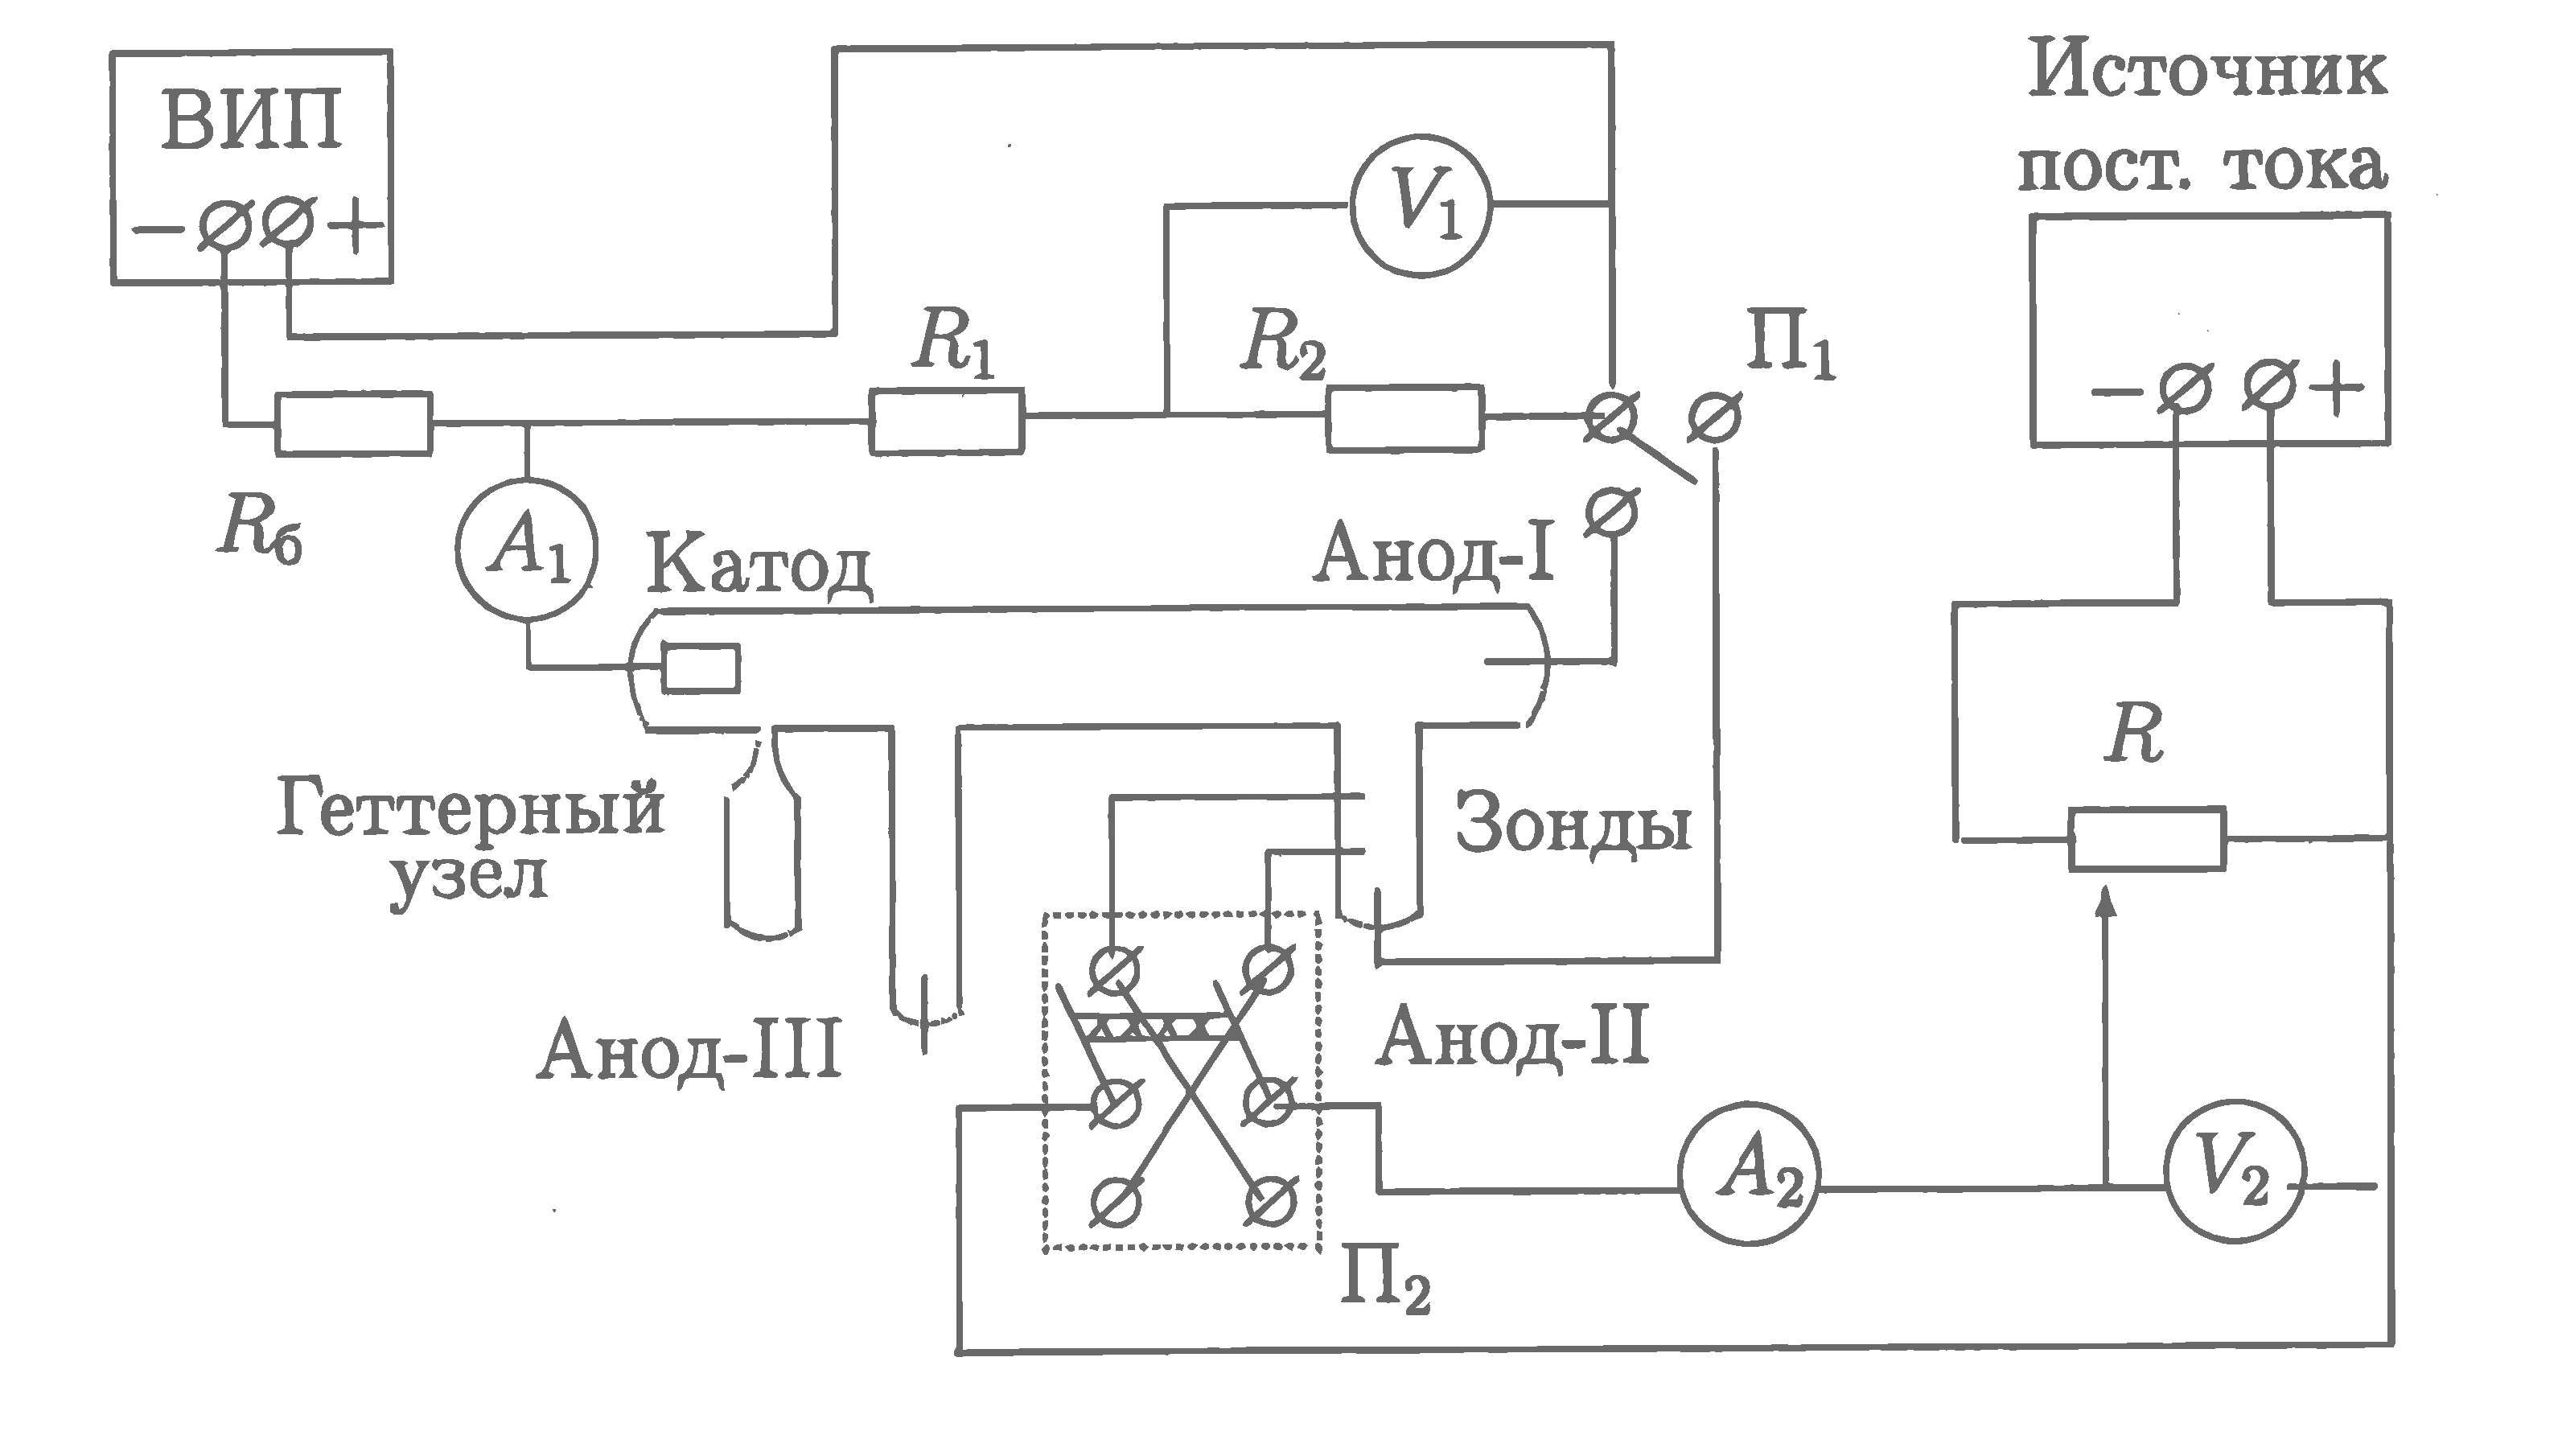
\includegraphics[width = 0.9\textwidth]{Chapter_5/3_5_1.eps}
	\caption{Схема установки для исследования газового разряда}
	\figmark{Neon gas discharge}
\end{figure}

При подключении к ВИП анода-I между ним и катодом возникает газовый разряд. Ток разряда измеряется миллиамперметром
$A_1$, а падение напряжения на разрядной трубке~--- цифровым вольтметром $V_{1}$, подключённым к трубке через
высокоомный (несколько десятков МОм) делитель напряжения с коэффициентом $(R_1+R_2)/R_2$.

При подключении к ВИП анода-II разряд возникает в~проcтранстве между катодом и анодом-II, где находится двойной зонд,
используемый для диагностики плазмы положительного столба. Зонды изготовлены из молибденовой проволоки диаметром
$d$ и имеют длину~$l$. Они подключены к источнику питания через потенциометр~$R$. Переключатель
$\text{П}_2$ позволяет изменять полярность напряжения на зондах. Величина напряжения на зондах изменяется с~помощью дискретного
переключателя <<$V$>> выходного напряжения источника питания и потенциометра $R$, а измеряется вольтметром~$V_2$. Для
измерения зондового тока используется микроамперметр~$A_2$.

Анод-III в нашей работе не используется.


\begin{lab:task}

В работе предлагается снять вольт-амперную характеристику тлеющего разряда и зондовые характеристики при разных токах
разряда и по результатам измерений рассчитать концентрацию и температуру электронов в плазме, степень ионизации,
плазменную частоту и дебаевский радиус экранирования.

 

\tasksection{Вольт-амперная характеристика разряда}

\begin{enumerate}
\item Установите переключатель $\text{П}_1$ в положение <<Анод-I>> и подготовьте приборы к работе согласно техническому описанию, которое находится в лаборатории. Плавно увеличивая выходное напряжение ВИП, определите напряжение зажигания разряда (показания вольтметра $V_{1}$ перед зажиганием). 

\item С помощью вольтметра $V_{1}$ и амперметра $A_{1}$ снимите вольт-амперную характеристику разряда $U_{1}=f(I_\text{р})$. Ток разряда $I_\text{р}$ изменяйте в диапазоне, указанном в описании работы в лаборатории (при больших токах может сгореть сопротивление).

\end{enumerate}

\tasksection{Зондовые характеристики}

\begin{enumerate}
\item Уменьшите напряжение ВИП до нуля, переведите переключатель~$\text{П}_1$
в~положение <<Анод-II>> и подготовьте приборы $\text{П}_{2}$, $V_{2}$ и $A_{2}$ к работе согласно техническому описанию, которое находится в лаборатории. 

\item Плавно увеличивайте напряжение ВИП до возникновения разряда. Установите значение разрядного
тока~$I_\text{р}$ согласно техническому описанию. Подготовьте к работе источник питания. После этого при помощи потенциометра $R$ установите на зонде максимальное напряжение $U_{2 max}$. 

\item Снимите вольт-амперную характеристику двойного зонда $I_{2}=f(U_{2})$ (в диапазоне от $-U_{2 max}$ до $U_{2 max}$) при фиксированном токе $I_\text{p}$ согласно описанию работы в лаборатории.

\item Повторите измерения при другой полярности (переключатель $\text{П}_2$). Менять полярность подключения зондов можно только при \important{нулевом токе}, поддерживая при этом величину тока разряда $I_\text{p}$ в трубке.

Записывая результаты в таблицу, одновременно стройте приближенный график $I=f(U)$  в тетради в интервале от $-U_{2 max}$ до~$U_{2 max}$. Отцентрируйте кривую: проведите ось абсцисс на уровне $I=\sum \Delta I/2$, восстановите ось ординат из точки пересения кривой с новой осью абсцисс. Убедитесь, что можно провести асимптоты к участкам кривой при больших напряжениях. Если точек мало --- проведите дополнительные измерения.

\item Снимите зондовые характеристики при токах разряда, равных 3 и 1,5~мА.
 \end{enumerate}

\tasksection{Обработка результатов}

 \begin{enumerate}

\item Постройте вольт-амперную характеристику разряда $U_{1}=f(I_\text{p})$. По наклону кривой определите максимальное дифференциальное сопротивление разряда $R_{max}$.

\item Постройте семейство зондовых характеристик $I=f(U)$ на одном листе.

\item По зондовым характеристикам определите температуру электронов~$T_{e}$ по формуле \chaptereqref{5.43}: ток $I_{i\text{н}}$ найдите из пересечения асимптоты к току насыщения с осью $U=0$; ($dI/dU)|_{U=0}$~--- наклон
характеристики~$I=f(U)$ в точке $U=0$, $I=0$; взяв $\Delta U$ в вольтах и приняв заряд электрона $e=1$, рассчитайте
энергию (<<температуру>>) электронов ($kT_{e}$) в электрон-вольтах.

\item Полагая концентрацию электронов $n_{e}$ равной концентрации ионов $n_{i}$, определите её из формулы \chaptereqref{5.31}:
\begin{equation}
	I_{i\text{н}}=0,4n_{e}eS\sqrt{\frac{2kT_{e}}{m_{i}}}.
\end{equation}

Здесь $S=\pi\cdot d\cdot l$~--- площадь поверхности зонда; значения $d$ и $l$ приведены в описании экспериментальной
установки; $m_i=22\cdot 1,66\cdot 10^{-24}$~г~--- масса иона неона.

\item Постройте графики $T_e=f(I_p)$, $n_e=f(I_p)$.

\item Рассчитайте плазменную частоту колебаний электронов по формуле:
\begin{equation}
	\omega_{p}=\sqrt{\frac{n_{e} e^2}{\varepsilon_{0} m_{e}} }.
\end{equation}

\item Рассчитайте дебаевский радиус~$r_{D}$ по формуле \chaptereqref{5.18}, которая в случае $T_{e}\gg T_{i}$ принимает в системе СИ вид
\begin{equation}
	r_{D}=\sqrt{\frac{\varepsilon_{0}kT_{i}}{ne^{2}}}.
\end{equation}

\item Оцените среднее число ионов в дебаевской сфере по формуле:
\begin{equation}
	N_{D}=\frac{4\pi}{3} n_{i}r_{D}^{3}.
\end{equation}

\item Оцените степень ионизации плазмы~$\alpha$ (долю ионизованных атомов), если давление в трубке $p\simeq 1$~мбар.

\item Оцените погрешности.

 \end{enumerate}

\end{lab:task}


\lab{Изучение плазмы индукционного газового разряда}

\aim{изучение свойств плазмы высокочастотного газового разряда
    в воздухе методом зондовых характеристик.}

\equip{газоразрядная трубка с высокочастотным генератором; источник
    постоянного тока; генератор звуковой частоты; электронный осциллограф;
    форвакуумный насос; вакуумметр; натекатель; вакуумный кран; делитель;
    повторители--фазовращатели.}

Перед выполнением работы необходимо ознакомиться с
теоретическим введением к разделу.
% Подробное описание свойств тлеющего разряда можно найти в Приложении к разделу
% (см. стр.~\pageref{sec:discharge}).

Ионизацию в плазме можно получить с помощью высокочастотных электромагнитных
переменных полей. Существуют различные способы введения ВЧ-поля
в разрядный объём. Один из них основан на использовании электромагнитной
индукции: через катушку-соленоид, в которую вставлена диэлектрическая
(например, стеклянная) газоразрядная камера, пропускается ток высокой частоты.
Внутри катушки индуцируется вихревое электрическое поле.
Силовые линии этого поля, а вместе с~ними и линии разрядного тока,
представляют собой окружности. Такой разряд  называется \term{кольцевым},
\term{индукционным} или разрядом $H$-типа, что указывает
на определяющую роль магнитного поля. 
Именно такой способ возбуждения газового разряда используется в нашей установке.

Другой способ возбуждения заключается в том, что на два электрода,
пространство между которыми заполнено разреженным газом,
подаётся высокочастотное переменное напряжение. 
Такие разряды называются \term{ёмкостными} или
разрядами $E$-типа.

Высокочастотные разряды широко используются в технике. Индукционные разряды
применяются в безэлектродных генераторах плотной низкотемпературной плазмы
(в плазмотронах), используемых, например, для плазмохимического производства
чистых веществ. Разряды ёмкостного типа применяются в мощных 
газоразрядных лазерах.

\paragraph{Механизм возникновения пробоя} 
В~высокочастотных разрядах --- как $H$- так и $E$-типа --- электроны
ускоряются под действием высокочастотного переменного электрического поля.

Предположим, что давление газа мало, так что столкновения электронов
с молекулами газа происходят редко. 
Ограничимся рассмотрением случая однородного поля, 
меняющегося по гармоническому закону: $\vec{E}=\vec{E}_0 \cos \omega t$, 
где $\vec{E}_0=\const$ --- амплитуда электрического поля. 
Эта задача была рассмотрена также в п.~\ref{sec:epsilon} (см. формулу \chaptereqref{free_E}).
Направив ось~$x$ вдоль~$\vec{E}_0$, получим
\[
    m_e\frac{d^2x}{dt^2}=-eE_0\cos\omega t.
\]
Интегрируя это уравнение, найдём скорость электрона:
\begin{equation*}
    v(t)=v_0+\frac{eE_0}{\omega m_e}\sin\omega t,
\end{equation*}
где $v_0$~--- начальная скорость.

Видно, что скорость электрона периодически меняется, 
но в среднем энергия электрона остаётся \emph{неизменной}. 
Так обстоит дело, пока газ достаточно разрежен. С~увеличением
давления соударения электронов с молекулами газа происходят всё чаще.
Однако если амплитуда напряжённости поля невелика,
легкие электроны не смогут ионизировать молекулы 
и будут соударятся с ними упруго, передавая им при этом
лишь малую долю своей энергии (поскольку масса электрона
много меньше массы молекулы).

Чтобы понять, как возникает зажигание разряда (пробой), рассмотрим
подробнее, что происходит при упругом соударении электрона с молекулами газа. 
Хотя энергия электрона при ударе об ион почти не меняется, 
направление его скорости претерпевает существенные изменения.
Если частота поля достаточно велика, новое направление
скорости электрона может совпасть с изменившимся за время соударения направлением 
электрического поля --- в таком случае электрон при
дальнейшем движении не возвращает полю энергию, а вновь её получает! 
Часть
электронов может поэтому ускоряться высокочастотным полем вплоть
до энергии ионизации, даже если амплитуда поля невелика. 
После ионизации процесс повторяется: при упругих столкновениях с молекулами газа 
часть электронов в электрическом поле ускоряется, вследствие чего 
происходят новые акты ионизации. 

Таким образом в газе накапливаются заряженные частицы --- электроны и ионы. По мере
увеличения их концентрации возрастает роль процессов \emph{рекомбинации}
(то есть объединения электрона и иона обратно в нейтральный атом). 
Отметим, что наблюдаемое свечение разряда есть в основном следствие именно рекомбинации
электронов и ионов.
В~результате
действия двух факторов~--- ионизации и рекомбинации~---
устанавливается стационарное состояние плазмы.
Её концентрация и температура зависят от сорта газа, его давления,
а также от частоты и амплитуды высокочастотного поля.


\experiment

Схема установки представлена на рис.~\figref{Induction gas discharge}.
Заполненная газом диэлектрическая камера представляет собой цилиндрическую
стеклянную трубку (ее диаметр и длина указаны в описании), на одном из торцов
которой впаяны две молибденовые проволочки (зонды)
диаметром~$d$ и длиной~$l$, расположенные на некотором расстоянии друг от друга.
Трубка вставлена в катушку индуктивности колебательного контура высокочастотного 
(ВЧ) генератора, 
работающего на частоте~$\sim10$~МГц. 
Камера закрыта экраном (металлической сеткой), защищающим измерительную
цепь зондов от высокочастотного поля.

\begin{figure}[h]
    \centering
    %    \footnotesize
    \pic{}{Chapter_5/c5_2_1}
    \caption{Схема установки для исследования газового разряда}
    \figmark{Induction gas discharge}
\end{figure}

Другой конец трубки не запаян и служит для откачки и для заполнения камеры газом. 
Камера откачивается форвакуумным насосом~(ФН), а давление в ней может
регулироваться с помощью натекателя, соединенного с атмосферой.
Значение давления контролируется термопарным вакуумметром.

\paragraph{Регулировка давления в системе}
Отметим важную особенность процедуры установки рабочего давления в
разрядной камере. Она осуществляется путем изменения
проходного сечения натекателя, соединенного с атмосферой, при 
\emph{непрерывной} работе откачивающего насоса. 
При этом скорость откачки сохраняется постоянной, а приток
воздуха в разрядную камеру определяется изменением аэродинамического
сопротивления натекателя. Таким образом, устанавливается новое значение
давления, при котором скорость откачки насоса уравновешивается расходом воздуха
через натекатель. Изменение сечения натекателя выполняется микрометрическим 
винтом, который сжимает расположенную под ним пружину и изменяет 
ее давление на подвижную
мембрану клапана. Такая система обладает очень большой \emph{инерционностью} и
реагирует на вращение винта со значительным запозданием.

\paragraph{Измерение зондовой характеристики}
Измерительная цепь зондов изображена на рис.~\figref{zond-measure}.
Две катушки~$L_{1}$ и~$L_{2}$, подключённые последовательно с зондами, 
не пропускают на осциллограф высокочастотный сигнал.
На зонды подаётся синусоидальное напряжение небольшой частоты 
($\sim$\,50~Гц) от звукового генератора~ЗГ.
Это же напряжение через делитель~Д и регулируемый 
повторитель-фазовращатель~ПФ2 подаётся на вход~$X$ электронного осциллографа
(ЭО). Последовательно с зондом подключён резистор~$R$ 
($R\sim 100\;КОм$, конкретное значение указано на установке),
напряжение на котором пропорционально току через зонды (т.\,е. через плазму).
Это напряжение подаётся на вход~$Y$ осциллографа 
через нерегулируемый повторитель-фазовращатель ПФ1. 

\begin{figure}[h!]
    \centering
    %    \footnotesize
    \pic{\textwidth}{Chapter_5/c5_2_2}
    \caption{Схема измерения зондовых характеристик в разряде}
    \figmark{zond-measure}
\end{figure}

На экране осциллографа наблюдается кривая, представляющая собой вольт-амперную
характеристику (ВАХ) двойного зонда (см. рис.~\chapterfigref{Double probe VAC}).
Регулируя амплитуду на звуковом генераторе, можно изменять диапазон значений
напряжения  на ВАХ. Из-за фазовых сдвигов, возникающих в измерительной цепи, 
картина на экране~ЭО~в общем случае имеет вид петли.
Для компенсации разности фаз и устранения этого эффекта 
используется регулятор фазовращателя ПФ2. Если регулировка ПФ2 не помогает,
следует изменить частоту ЗГ.

По пересечению асимптот зондовой характеристики с осью ординат
можно определить ионный ток насыщения зондов $I_{iн}$, а по наклону 
характеристики вблизи начала координат~--- электронную температуру $T_e$
(см. п.~\ref{sec:double} Введения к разделу).




\begin{lab:task}

\taskpreamble{В~работе предлагается при различных давлениях газа в~трубке получить зондовые
вольт-амперные характеристики на экране
осциллографа и рассчитать с~их помощью температуру и~концентрацию электронов
в~плазме, степень ионизации, плазменную
частоту и дебаевский радиус экранирования.}

\tasksection{Подготовка к работе}

\item До включения приборов ознакомьтесь с установкой по техническому описанию 
в лаборатории.

\item Подготовьте к работе термопарный вакуумметр (см. техническое описание). 
Включите форвакуумный насос и вакуумметр. 
Откачайте трубку до давления $P\sim 10^{-1}\div 10^{-2}$~торр (рекомендованные
значения см. в техническом описании). Давление
регулируется с~помощью натекателя (микровентиля) при непрерывной работе
насоса.

\begin{lab:warning}
    Не выключайте насос до конца работы!
\end{lab:warning}

\item Включите источник питания ВЧ-генератора. Убедитесь, что
в трубке возник разряд: после зажигания он должен устойчиво гореть 
по всей трубке, включая область расположения зондов.

\item  Включите осциллограф и звуковой генератор. 
%При этом на зонды подается
%переменное напряжение от генератора с частотой, указанной в описании в лаборатории.
Подберите напряжение на генераторе, при котором на экране осциллографа 
появится кривая, похожая на теоретическую зависимость, изображённую на
рис.~\chapterfigref{Double probe VAC}.
Выходное напряжение генератора должно быть таким, чтобы на кривой 
наблюдались начальные участки области насыщения (асимптоты ВАХ).

Если вместо кривой на экране возникает петля, воспользуйтесь ручкой 
регулировкой фазовращателя ПФ2. Если регулировка не помогает, следует 
изменить частоту генератора.

При чрезмерно большом напряжении генератора
возникает искажение зондовой характеристики, в ее оконечных областях появляются
изломы и <<выпучины>>. Это происходит вследствие влияния электрического поля зондов
на характер плазменного разряда. Такого допускать не следует, уменьшая
при необходимости напряжение питания зондов до исчезновения искажений.


\item \label{p521} Посмотрите, как ведёт себя разряд, насколько он устойчив при изменении
давления в рабочем диапазоне. Проверьте, что наблюдаемая 
на экране кривая в целом соответствует теоретической.

\tasksection{Измерения}

\item Получите на экране осциллографа вольт-амперную характеристику зондов
(см. рис.~\chapterfigref{Double probe VAC}) для максимального давления из
выбранного диапазона.

\item Регулируя напряжение звукового генератора и коэффициент усиления 
осциллографа по осям~$X$ и $Y$ (вольт/деление), 
добейтесь того, чтобы кривая занимала большую часть экрана. 

Если у осциллографа есть ручка плавной регулировки масштаба
(например, осциллограф GOS-620), убедитесь, что она находится в 
<<калиброванном>> положении, при котором чувствительность каналов 
соответствует положению дискретного переключателя усиления.

\item Зафиксируйте изображение кривой с экрана осциллографа 
(сфотографируйте или зарисуйте с~экрана на кальку). 
Запишите давление в системе $P$ и чувствительность осциллографа по 
осям~$X$ и~$Y$.

\item Повторите измерения для 5--6 значений давления внутри диапазона, 
в котором зондовая характеристика соответствует теоретической
(см. п. \ref{p521}).

\item Закончив работу, выключите сначала насос и \textbf{сразу же откройте натекатель}
(для предотвращения выдавливания масла из насоса).
Затем отключите вакуумметр и остальные приборы.

\item Перепишите параметры установки: сопротивление датчика тока~$R$, коэффициент
делителя~Д, геометрические характеристики зондов и разрядной трубки.

\tasksection{Обработка результатов}

\item По значению сопротивления $R$, с которого подавался
сигнал на канал~$Y$ осциллографа  (см. рис.~\figref{zond-measure}), 
для каждой кривой пересчитайте масштабы по оси~$Y$ из единиц
напряжения в единицы тока.
 
Рассчитайте масштаб по оси~$X$ с учётом наличия делителя~Д в канале 
зондового напряжения.

\item По зондовым характеристикам определите температуру~$T_e$ электронов
(см. п. \ref{sec:double} Введения). Ответ
выразите в энергетических единицах (электрон-вольтах).

\item По зондовым характеристикам определите значения ионных токов насыщения
зондов $I_{iн}$. 
Определите концентрацию $n$ электронов и ионов в плазме, 
считая ионы однозарядными ($Z=1$).
Площадь поверхности зонда (в пренебрежении
дебаевским слоем): $S\approx \pi d l$, где 
$d$~--- диаметр, $l$~--- длина зонда.

\item Рассчитайте плазменную частоту колебаний электронов $\omega_p$,
электронную поляризационную длину~$r_{De}$ и дебаевский радиус экранирования~$r_D$
(с учётом того, что температура ионов мала по сравнению с электронной: $T_i\ll T_e$). 
Можно ли считать плазму квазинейтральной?

\item Оцените среднее число ионов в дебаевской сфере $N_D$. 
Является ли плазма разряда идеальной?

\item Оцените степень ионизации плазмы (долю ионизованных атомов $\alpha$)
для каждого давления~$P$ в трубке.

\item Оцените погрешности эксперимента.

\end{lab:task}

\begin{lab:questions}
    \item Дайте определение понятия <<плазма>>. Назовите различные виды плазм в лаборатории, 
    технике и природе.
    
    \item Что такое дебаевская длина экранирования? Выведите формулу
    для дебаевской длины в одномерном случае для равновесной плазмы.
    
    \item Что такое плазменная частота? Выведите формулу для плазменной частоты.
    Какие процессы в плазме характеризуются плазменной частотой?

    \item Что такое равновесная и неравновесная плазма? 
    Является ли исследуемая в работе плазма равновесной?
        
    \item Чем определяется потенциал зонда, погружённого в плазму? 
    Чем определяется зондовый ток насыщения для одиночного зонда? Для двойного
    зонда?
    
    \item Каков механизм зажигания разряда в высокочастотном поле?
    
    \item Для чего нужны защитный экран вокруг разрядной трубки и катушки $L_1$, $L_2$ в измерительной
    цепи зонда?
\end{lab:questions}







\cleardoublepage
\chapter{Спектральный анализ}

Задача описания поведения некоторой системы во времени сводится к выяснению связи
межу~<<сигналом>>, подаваемым на <<вход>> системы (обозначим его как $f(t)$),
и её реакцией на <<выходе>> ($g(t)$):
\begin{equation*}
f(t)\to\fbox{?} \to g(t).
\end{equation*}
В этой главе мы рассмотрим \important{спектральный} метод решения данной задачи применительно
к \important{линейным} системам.

\begin{wrapfigure}[10]{o}{0.3\textwidth}
% \psfragfig[width=0.25\textwidth]{Images/Chapter_6/1}{%
%     \psfrag{f}[cc]{$f(t)$}
%     \psfrag{g}[cl]{$g(t)$}
%     \psfrag{r}[ct]{$R$}
%     \psfrag{c}[cr]{$C$}
%     \psfrag{l}[cb]{$L$}}
    \centering
    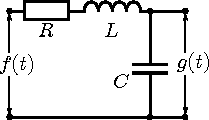
\includegraphics[scale=0.9]{Chapter_6/v6-RLC.pdf}
    \caption{Входной и выходной сигналы в $RLC$-контуре}
    \figmark{RLC circuit}
\end{wrapfigure}

Прежде, чем излагать теорию в общем виде, рассмотрим конкретный пример.
Пусть на вход колебательного $RLC$-кон\-ту\-ра подано некоторое
напряжение $U_{вх}=f(t)$. Будем снимать напряжение с конденсатора:
$U_{вых}=U_C = g(t)$. Попробуем выяснить, как связаны~$f(t)$ и~$g(t)$.

Ответ хорошо известен, если $f(t)$~--- гармоническая функция некоторой частоты~$\omega$.
Пусть в комплексном представлении $f(t)=c e^{i\omega t}$, где~$c$~---
комплексная амплитуда сигнала ($c=ae^{i\varphi}$, где~$a$~--- амплитуда,
$\varphi$~--- фаза). Тогда, как известно, $g(t)$ будет гармонической
функцией с той же частотой: $g(t)=g_0 e^{i\omega t}$, где~$g_0$
нетрудно найти методом комплексных амплитуд (см. Гл.~2, а также
Пример~\ref{example:RLC} ниже).
% \begin{equation*}
%  g_0 = \frac{Z_C}{R+Z_C+Z_L}c_0,
% \end{equation*}
% где $Z_C=\frac{1}{i\omega C}$~--- импеданс конденсатора,
% $Z_L=i\omega L$~--- импеданс катушки.
Отклик будет пропорционален амплитуде входного сигнала, и в
абстрактной форме ответ можно записать как
\begin{equation*}
g_0 = c\lambda(\omega)
\end{equation*}
где~$\lambda(\omega)$ --- зависящий от частоты комплексный коэффициент,
называемый \term{частотной характеристикой}
(или \term{функцией отклика}) системы.

Можем ли мы, зная вид частотной характеристики $\lambda(\omega)$, установить
связь между входным $f(t)$ и выходным $g(t)$ сигналами при \important{произвольном} $f(t)$?

Важнейшим свойством рассматриваемого колебательного контура, позволяющим
дать утвердительный ответ на поставленный вопрос, является
\term{линейность} законов, которые описывают его состояние.
Линейными называют системы, для которых справедлив \term{принцип суперпозиции}:
если $g_1$ --- отклик системы на воздействие $f_1$, а $g_2$ --- на воздействие
$f_2$, то откликом на сумму воздействий $f_1 + f_2$ будет также сумма $g_1 + g_2$.

Как известно, состояние колебательного контура подчиняется
\important{линейному дифференциальному уравнению второго порядка}:
\begin{equation*}
L\ddot{q} + R\dot{q} + q/C=f(t),
\end{equation*}
где $q(t)$ --- заряд на конденсаторе. Очевидно, что дифференцирование ---
линейная операция (а также сложение и домножение на константу),
% Для данного уравнения нетрудно доказать
% справедливость принципа суперпозиции (см. курсы дифференциальных уравнений),
поэтому $RLC$-контур действительно являет собой частный случай линейной системы.

Пусть $f(t)$~--- сумма некоторого числа гармонических функций с разными частотами:
\begin{equation*}
f(t) = \sum\limits_n c_n e^{i\omega_n t},
\end{equation*}
где $c_n$ --- набор некоторых (комплексных) коэффициентов.
Линейность системы позволяет найти её отклик $g(t)$.
Отклик на каждое слагаемое есть
\begin{equation*}
 g_n = c_n\lambda(\omega_n)
\end{equation*}
и в сумме имеем
\begin{equation*}
g(t) = \sum\limits_n  c_n \lambda (\omega_n) e^{i\omega_n t}.
\end{equation*}
Мы видим, что рассматриваемый колебательный контур некоторым образом
преобразует гармонические компоненты, содержащиеся во входном сигнале.
В частности, он может подавлять одни частоты и усиливать другие.
Можно сказать, что он выполняет роль \term{частотного фильтра}.

Если произвольную функцию $f(t)$ удастся представить в виде
некоторой суммы (конечной или бесконечной) гармонических слагаемых, то
задача о связи воздействия и отклика системы будет решена.
Такое разложение называют \term{спектральным}.


\introsection{Линейные фильтры. Частотная характеристика}

Итак, назовём \term{линейным фильтром} систему,
преобразующую внешнее воздействие $f(t)$ в некоторый отклик $g(t)$,
и подчиняющуюся \important{принципу суперпозиции}.

Изобразим произвольный линейный фильтр с помощью блок-схемы:
\begin{equation*}
    f(t)\to\fbox{$\hat\Lambda$} \to g(t),
\end{equation*}
где $f(t)$~--- внешнее воздействие (<<входной сигнал>>, например, внешняя
ЭДС, действующая на колебательный контур), $g(t)$~--- выходной сигнал
(отклик фильтра, например, напряжение на конденсаторе контура).
Эту связь можно также обозначить как
\begin{equation*}
g=\hat\Lambda [f],
\end{equation*}
где $\hat\Lambda$~--- некоторое линейное преобразование (<<оператор>>),
преобразующее входной сигнал $f(t)$ в выходной сигнал $g(t)$.
Свойство его линейности (принцип суперпозиции) можно записать в
виде равенства
\begin{equation*}
\hat\Lambda [c_1f_1+c_2f_2]=c_1\cdot \hat \Lambda [f_1]+c_2\cdot \hat \Lambda [f_2],
\end{equation*}
которое должно выполняться для любы функций $f_1(t)$ и $f_2(t)$ и
для любых комплексных констант $c_1$ и $c_2$.

Мы будем рассматривать далее линейные \important{стационарные} фильтры, т.~е.
фильтры с постоянными, не зависящими от времени параметрами (например, $L$, $C$, $R$).

Из свойства линейности следует простое правило для нахождения
отклика фильтра на \important{произвольное} внешнее воздействие $f(t)$.
Необходимо представить это воздействие в виде суперпозиции некоторых
<<элементарных>> слагаемых $f(t)=\sum c_n f_n$, а затем найти отклик на каждое
слагаемое $g_n = c_n \cdot \hat \Lambda f_n$. Окончательный результат
получается суммированием откликов: $g(t)=\sum c_n \hat\Lambda f_n$.
В этом состоит суть \term{спектрального метода} решения задачи
нахождения отклика линейной системы на внешнее воздействие.

Выбор элементарных слагаемых --- \term{базиса} --- неоднозначен.
Естественно попытаться разложить внешнее воздействие на такие
слагаемые, отклик на которые находится наиболее простым образом. Такими
слагаемыми являются так называемые
\term{собственные функции фильтра}, т.\,е. функции $\psi_n(t)$,
удовлетворяющие равенству
\begin{equation}
    \hat \Lambda[\psi_n]=\lambda_n \psi_n.
\end{equation}
Это равенство означает, что, если внешнее воздействие описывается собственной
функцией, то отклик описывается той же функцией с некоторым множителем
$\lambda_n$, который математики называют \term{собственным значением}.

Для линейных стационарных фильтров, которые подчиняются линейным
дифференциальным уравнениям (например, колебательный контур),
такими собственными функциями являются функции $e^{i\omega t}$~--- гармонические
колебания (в комплексной форме):
\begin{equation*}
\hat\Lambda\left[e^{i\omega t}\right]=\lambda(\omega)e^{i\omega t},
\end{equation*}
где $\lambda(\omega)$ --- комплексная функция частоты, которая, напомним,
называется \term{частотной характеристикой} фильтра.
Действительно, для операции дифференцирования $n$-го порядка справедливо
$\left(\frac{d}{dt}\right)^n e^{i\omega t} = (i\omega)^n e^{i\omega t}$.
Поэтому частотная характеристика $\lambda(\omega)$ дифференциального уравнения
с постоянными коэффициентами будет в общем случае некоторой рациональной
функцией от $i\omega$.

\begin{lab:example}\label{example:RLC}
Найдём частотную характеристику $\lambda(\omega)$ фильтра,
изображённого на рис.~\figref{RLC circuit} ($RLC$-контура).

Частотная характеристика определяет отклик на входной гармонический сигнал
единичной амплитуды~--- внешнюю ЭДС $f_0(t)=e^{i\omega t}$.
Закон Кирхгофа:
\begin{equation}
    \eqmark{RLC}
L\ddot{q} + \dot{q}R+\frac{q}{C}=e^{i\omega t}.
\end{equation}
Для выходного сигнала $g(t)=\frac{q}{C}$ получаем уравнение
\begin{equation*}
\ddot{g}+2\gamma\dot{g}+\Omega^2g=\Omega^2 e^{i\omega t},
\end{equation*}
где $\gamma = R/2L$ --- коэффициент затухания,
$\Omega = 1/\sqrt{LC}$ ---- частота свободных колебаний.
Ищем решение в виде
\begin{equation*}
g(t)=\lambda(\omega)e^{i\omega t}.
\end{equation*}
Подставляя в исходное уравнение, имеем
\begin{equation*}
    (-\omega^2 +2i\omega\gamma + \Omega^2) \lambda e^{i\omega t}=\Omega^2 e^{i\omega t}.
\end{equation*}
Окончательно находим:
\begin{equation}
    \eqmark{RLC-lambda}
\begin{gathered}
\lambda(\omega)=\frac{\Omega^2}{\Omega^2-\omega^2+i2\gamma\omega},\\
\left|\lambda(\omega)\right|=\frac{\Omega^2}{\sqrt{
(\Omega^2-\omega^2)^2+4\gamma^2\omega^2}},
\qquad \varphi(\omega)=\arctg\frac{2\gamma\omega}{\omega^2-\Omega^2}.
\end{gathered}
\end{equation}
\end{lab:example}

\begin{wrapfigure}[14]{o}{0.25\textwidth}
\centering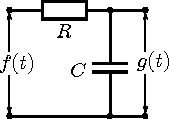
\includegraphics[scale=0.8]{Chapter_6/v6-RC.pdf}
\caption{\footnotesize Интегрирующая $RC$-цепочка}
\figmark{RC}
\end{wrapfigure}

\begin{lab:example}\label{example:RC}
Найдём частотную характеристику $RC$-цепочки (рис.~\figref{RC}).
Повторяя рассуждения из Примера~\ref{example:RLC} при $L=0$, получим
\begin{equation*}
\lambda(\omega) = \frac{1}{1+i\omega \tau_C},
\end{equation*}
где $\tau_C=RC$ --- постоянная времени $RC$-цепочки.

При $\omega \gg 1/\tau_C$ имеем $\lambda \approx \frac{1}{i\omega\tau_C} \to 0$,
то есть $RC$-цепочка является простейшим \important{фильтром высоких частот}.

В этом пределе можно выразить результат действия цепочки в явном виде.
При $\omega\tau_C\gg1$ напряжение на конденсаторе $q/C$ мал\'{о} по сравнению
с напряжением $\dot{q}R$ на резисторе, поэтому
\begin{equation*}
\dot{q} R \approx f(t) \qquad \to \qquad g(t) = \frac{q}{C} = \frac{1}{\tau_C}\int\limits_0^t f(t')\,dt'.
\end{equation*}
Таким образом, фильтрация высокочастотных гармоник сводится к интегрированию
входного сигнала (подумайте, почему интеграл от быстропеременной функции
по достаточно большому интервалу оказывается мал).
\end{lab:example}

\introsection{Спектральное разложение}

Итак, при изучении линейных систем (фильтров) возникает необходимость
представления произвольного сигнала $f(t)$ в виде
\begin{equation}
    \eqmark{Fourier series}
    f(t)=\sum\limits_n c_n e^{i\omega_n t}.
\end{equation}
Представление \eqref{Fourier series} называется разложением сигнала~$f(t)$ в
\term{ряд Фурье}, а отдельные слагаемые ряда (составляющие
гармонические колебания) $c_n e^{i\omega_n t}$ называют \term{гармониками}.
Совокупность коэффициентов~$\{c_n\}$ называется \term{спектром} функции~$f(t)$.
Коэффициент~$c_n$ представим в виде $c_n=a_ne^{i\varphi_n}$, где
модуль $a_n=|c_n|$ определяет \important{амплитуду} гармоники частоты~$\omega_n$,
а аргумент $\varphi_n=\arg c_n$~--- \important{начальную фазу}.

В курсах математического анализа доказывается, что
разложение~\eqref{Fourier series} может быть осуществлено в общем случае (при
некоторых физически несущественных
ограничениях на~$f(t)$), причем \important{единственным} образом.
То есть, существует единственный набор необходимых частот~$\omega_n$ и
единственный набор отвечающих этим частотам амплитуд~$a_n$ и фаз~$\varphi_n$,
обеспечивающих представление функции~$f(t)$ в виде суперпозиции гармонических
функций. Соответствующие формулы для этих коэффициентов мы получим ниже.

Отметим важное свойство гармонических функций.
Колебание $e^{i\omega_0 t}$ частоты~$\omega_0$ не может быть
представлено суперпозицией гармонических колебаний $\sum c_n e^{i\omega_n t}$
других частот $\omega_n\ne\omega_0$, какие бы коэффициенты~$c_n$, т.\,е.
амплитуды и фазы слагаемых гармоник, мы ни подбирали. В~математике это
свойство называют \term{ортогональностью}: функция $e^{i\omega_0 t}$
не имеет <<проекции>> на любую другую функцию $e^{i\omega_nt}$ при
$\omega_0\ne\omega_n$ (подобно тому как вектор, параллельный оси~$z$,
невозможно представить в виде суммы векторов, параллельных осям~$x$ и~$y$).

Для \important{действительных} функций $f(t)$, которые как правило и представляют интерес,
наряду с разложением \eqref{Fourier series} часто используется разложение
в ряд Фурье вида%
\footnote{Также можно использовать эквивалентное разложение
\begin{equation*}f(t)=\sum\limits_{n=0}^{\infty} A_n \cos(\omega_n t) + B_n \sin(\omega_n t),\end{equation*}
где $a_n=\sqrt{A_n^2+B_n^2}$, $\tg \varphi_n = \frac{B_n}{A_n}$.}
\begin{equation}
    \eqmark{Fourier-real-valued function}
    f(t)=\sum\limits_{n=0}^{\infty} a_n \cos(\omega_n t+\varphi_n ),
\end{equation}
где $a_n$, $\varphi_n$~--- действительные константы. Найдём связь между
коэффициентами разложений \eqref{Fourier series} и \eqref{Fourier-real-valued function}.
Пользуясь формулой Эйлера
\begin{equation}
    \eqmark{euler}
    \cos\alpha=\frac{e^{i\alpha}+e^{-i\alpha}}{2},
\end{equation}
представим каждое слагаемое \eqref{Fourier-real-valued function} в виде
\begin{equation*}
    a_n\cos(\omega_nt+\varphi_n)=\frac{a_n}{2}e^{i\varphi_n}\,e^{i\omega_n
t}+\frac{a_n}{2}e^{-i\varphi_n}\,e^{-i\omega_n t},
\end{equation*}
откуда ясно, что разложения \eqref{Fourier series} и
\eqref{Fourier-real-valued function} будут тождественны, если суммирование в
\eqref{Fourier series} проводить как по положительным частотам~$\omega_n$
(имеющим понятный физический смысл), так и по отрицательным (формально введённым)
частотам $\omega_{-n}=-\omega_n$, причём соответствующие коэффициенты имеют вид
\begin{equation}
    \eqmark{Fourier-coefficient}
    c_n =\frac{1}{2}a_n e^{i\varphi_n},
    \qquad c_{-n}=\frac{1}{2}a_n e^{-i\varphi_n}
\end{equation}
(коэффициенты $c_{-n}$ соответствуют отрицательным частотам~$-\omega_n)$,
т.\,е каждому слагаемому $a_n\cos(\omega_nt+\varphi_n)$ ряда \eqref{Fourier series}
соответствуют два слагаемых $c_ne^{i\omega_n t}$ и
$c_{-n}e^{-i\omega_n t}$ ряда \eqref{Fourier-real-valued function}.
% Нетрудно получить формулы обратного перехода от $\{c_n\}$ к
% $\{a_n,\varphi_n\}$:
% \begin{equation}
%      \eqmark{Fourier-coefficient-reverse}
%     a_n = 2|c_n|\qquad \varphi_n = \arg c_n.
% \end{equation}


Мы видим, что при разложении \important{действительных} функций~$f(t)$ в ряд Фурье
коэффициенты разложения~$c_{-n}$ на отрицательных
частотах связаны с коэффициентами~$c_n$ простым соотношением
\begin{equation*}
c_{-n}=c_{n}^*,
\end{equation*}
где звёздочка обозначает \important{комплексное сопряжение}.
Таким образом, гармоники с отрицательными частотами не несут какой-либо
дополнительной информации о действительном сигнале~$f(t)$.

Спектр функции~$f(t)$ принято изображать в виде графика
(рис.~\figref{spectrum}): длина стрелочки на каждой частоте~$\omega_n$
определяется модулем коэффициента~$c_n$ (т.~е. амплитудой соответствующего
гармонического колебания). Следует указать также начальные фазы~$\varphi_n$
спектральных компонент.

\begin{figure}[ht]
%     \psfragfig[width=0.7\textwidth]{Images/Chapter_6/7}{%
%     \psfrag{a}[ct]{$\omega_1$}
%     \psfrag{b}[ct]{$\omega_2$}
%     \psfrag{c}[ct]{$\omega_3$}
%     \psfrag{d}[ct]{$\omega_4$}
%     \psfrag{e}[ct]{$-\omega_{1}$}
%     \psfrag{f}[ct]{$-\omega_{2}$}
%     \psfrag{g}[ct]{$-\omega_{3}$}
%     \psfrag{h}[ct]{$-\omega_{4}$}
%     \psfrag{o}[ct]{0}
%     \psfrag{1}[cb]{$\varphi_1$}
%     \psfrag{2}[cb]{$\varphi_2$}
%     \psfrag{3}[cb]{$\varphi_3$}
%     \psfrag{4}[cb]{$\varphi_4$}
%     \psfrag{x}{$\omega$}
%     \psfrag{y}{$\{c_n\}$}
%     \psfrag{z}{$\{a_n\}$}
%     \psfrag{A}{а)}
%     \psfrag{B}{б)}}
    \centering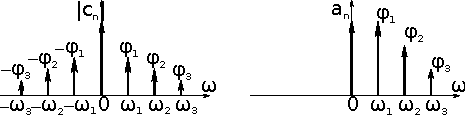
\includegraphics{Chapter_6/v6-cmplx-vs-real.pdf}
    \caption{Спектр в комплексном (слева) и действительном (справа) представлениях}
    \figmark{spectrum}
\end{figure}

Пример разложения \eqref{Fourier-real-valued function} (в ряд
косинусов) представлен на графике рис. \figref{spectrum} (справа): здесь нет
отрицательных частот, а длины стрелочек на положительных частотах в соответствии с
\eqref{Fourier-coefficient} удваиваются. При этом постоянные составляющие
(на частоте $\omega=0$) в разложениях \eqref{Fourier series} и
\eqref{Fourier-real-valued function} одинаковы: $a_0=c_0$.

\introsubsection{Спектр периодического процесса}\label{sec:spectrum-periodic}
Получим коэффициенты разложения в ряд Фурье для периодического колебательного
процесса общего вида $f(t)=f(t+T)$, где $T$~--- период процесса.
Покажем, что в этом случае функция~$f(t)$ может быть представлена
бесконечной суммой гармонических колебаний с кратными частотами~$\omega_n=n\omega_0$,
где $\omega_0=2\pi/T$, $n$~--- целое число:
\begin{equation}
    \eqmark{Fourier-periodic osc}
    f(t)=\sum_{n=-\infty}^{\infty} c_n e^{in\omega_0 t}.
\end{equation}
Нетрудно видеть, что все слагаемые в \eqref{Fourier-periodic osc}~---
периодические функция с периодом, кратным $T$, и они полностью исчерпывают
набор гармонических функций, удовлетворяющих условию $f(t)=f(t+T)$.
Таким образом, периодическая функция имеет \term{дискретный}
спектр с кратными частотами.

Спектр --- то есть набор коэффициентов~$\{c_n\}$ ---
можно найти следующим образом: домножим обе части равенства
\eqref{Fourier-periodic osc} на $e^{-im\omega_0 t}$ и
проинтегрируем по времени~$t$ за период (например от~$0$ до~$T$). Получим
\begin{equation*}
    \int\limits_{0}^{T} f(t)e^{-im\omega_0t}\,dt=\sum_n c_n\int\limits_{0}^{T}
e^{i(n-m)\omega_0 t}\,dt.
\end{equation*}
Вычислим интеграл в правой части:
\begin{equation*}
    \int\limits_{0}^{T}e^{i(n-m)\omega_0 t}dt =
%     = \left.\frac{e^{i(n-m)\omega_0 t}}{i(n-m)\omega_0} \right|_0^{T}
    \begin{cases}
        0 & \text{при~}n\ne m,\\
        T & \text{при~}n = m.
    \end{cases}
\end{equation*}
% (время $T$ есть целое число периодов колебания функций
% $\cos(n-m)\omega_0t$ и $\sin(n-m)\omega_0t$, поэтому интегралы от них
% на отрезке $[0,\,T]$ зануляются).
Таким образом, находим
\begin{equation}
    \eqmark{fourier-coeff}
    c_n=\frac{1}{T}\int\limits_{0}^{T} f(t)e^{-in\omega_0 t}\,dt.
\end{equation}
Это и есть искомое правило нахождения коэффициентов разложения периодической
функции в гармонический ряд Фурье.

\begin{wrapfigure}[10]{o}{0.5\textwidth}
%     \psfragfig[width=0.5\textwidth]{Images/Chapter_6/12}{%
%     \psfrag{x}{$t$}
%     \psfrag{1}[rb]{1}
%     \psfrag{f}{$f(t)$}
%     \psfrag{a}[cb]{$\tau$}
%     \psfrag{b}[cb]{$T$}}
    \centering
    \includegraphics[width=0.5\textwidth]{Chapter_6/12}
    \caption{Периодическая последовательность импульсов}
    \figmark{meander}
\end{wrapfigure}

\begin{lab:example}\label{example:square-zug}
Найдём спектр периодической последовательности прямоугольных
импульсов длительности~$\tau$ с периодом следования импульсов $T>\tau$
(рис.~\figref{meander}, начало отсчёта выбрано так, что~$f(t)$ --- чётная
функция).

Используя \eqref{fourier-coeff} на интервале интегрирования
$-T/2\le t \le T/2$, с учётом того, что функция~$f(t)$ отлична от нуля и
равна единице лишь в области $|t|<\tau/2$, находим
\begin{equation}
    \eqmark{impulses-spectrum}
    c_n =\frac{1}{T}\int\limits_{-\tau/2}^{\tau/2} e^{-in\omega_0 t}\,dt
    =\frac{\tau}{T}\cdot \frac{\sin \left(n\omega_0\tau/2\right)}{n\omega_0\tau/2} =
     \frac{\sin \left(\pi n \tau/T\right)}{\pi n}.
\end{equation}

\begin{figure}[h!]
%     \psfragfig[width=\textwidth]{Images/Chapter_6/13}{%
%     \psfrag{x}{$\omega$}
%     \psfrag{y}{$c_n$}
%     \psfrag{0}[tr]{0}
%     \psfrag{1}[ct]{$\vphantom{2}\omega_0$}
%     \psfrag{2}[ct]{$2\omega_0$}
%     \psfrag{c}{$C(\omega)$}
%     \psfrag{d}[ct]{$2\Delta\omega$}}
    \centering
%    \includegraphics[width=0.9\textwidth]{Chapter_6/13.pdf}
    \pic{0.7\textwidth}{Chapter_6/13}
    \caption{Спектр периодической последовательности импульсов
        (рисунок приведён для случая $\tau=\frac13 T$)}
    \figmark{spectrum-meander}
\end{figure}

Спектр $\{c_n\}$ показан на рис.~\figref{spectrum-meander}.
Пунктирной кривой изображена огибающая функция
\begin{equation*}
    C(\omega) =\frac{\tau}{T}\cdot \frac{\sin\omega\tau/2}{\omega\tau/2}.
\end{equation*}
При $\omega=n\omega_0$ эта функция принимает значение $C(n\omega_0)=c_n$.
Полуширина $\Delta \omega$ главного максимума этой функции определяется
условием $\sin\omega\tau/2=0$:
\begin{equation*}
    \Delta\omega \cdot \frac{\tau}{2}=\pi\qquad \text{или} \qquad \Delta \omega
\cdot \tau =2\pi.
\end{equation*}
Как видно из рисунка, спектральные гармоники,
имеющие заметную амплитуду, сосредоточены в интервале частот
$|\omega|\lesssim\Delta\omega=2\pi/\tau$.
\end{lab:example}


\introsubsection{Спектр непериодического процесса}

Рассмотрим задачу разложения в спектр произвольного непериодического
сигнала $f(t)$.

Ответ можно получить, воспользовавшись результатом
\eqref{fourier-coeff} для разложения периодической функции
и устремляя период к бесконечности $T\to \infty$.

\begin{wrapfigure}[9]{o}{0.5\textwidth}
    \centering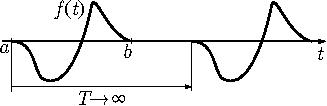
\includegraphics[width=\linewidth]{Chapter_6/v6-finf.pdf}
    \caption{Непериодический процесс как предел периодического}
    \figmark{finf}
\end{wrapfigure}

Пусть функция $f(t)$ отлична от нуля на некотором конечном интервале
$t\in[a,\,b]$, а вне его обращается в ноль. Рассмотрим периодическую функцию
с достаточно большим периодом повторения $T>b-a$, составленную из <<кусков>>
функции $f(t)$. Посмотрим, что происходит со спектральным разложением
такой функции по мере увеличения $T$.

Видно, что частоты $\omega = n \frac{2\pi}{T}$ гармоник, по которым идёт
разложение, будут в пределе $T\to \infty$ располагаться всё плотнее друг к другу.
Интервал между соседними частотами равен $\Delta \omega = \frac{2\pi}{T}$.
Таким образом, имеем $\Delta \omega\to 0$ и, следовательно,
спектр должен стать \term{непрерывным}.

Тогда спектральное разложение превратится из суммы в интеграл:
\begin{equation*}
 f(t) = \frac{1}{\Delta \omega}\sum c_n e^{i\omega_n t} \Delta \omega \to
 \frac{T}{2\pi} \int\limits_{-\infty}^{\infty} c_n e^{i\omega_n t} d\omega,
\end{equation*}
Обозначая $C(\omega)=c_n T$, запишем искомое разложение как
\begin{equation}
\eqmark{Fourier integral}
f(t) = \frac{1}{2\pi} \int\limits_{-\infty}^{\infty} C(\omega) e^{i\omega t} d\omega,
\end{equation}
где $C(\omega)$ найдём из \eqref{fourier-coeff}:
\begin{equation}
\eqmark{Fourier integral-coef}
 C(\omega) =
%  \frac{c_n}{\Delta \omega} =
%  \frac{1}{\Delta \omega T}\int\limits_{-\infty}^{\infty}
%  f(t) e^{-i\omega t} dt \to
\int\limits_{-\infty}^{\infty} f(t) e^{-i\omega t} dt.
\end{equation}

Множитель $C(\omega)=a(\omega)e^{i\varphi(\omega)}$ показывает, с каким
<<весом>> (т.~е. с какой амплитудой $a(\omega)$ и с какой начальной фазой
$\varphi(\omega)$) необходимо складывать гармонические
колебания разных частот, чтобы при суммировании (интегрировании) образовать
заданный сигнал $f(t)$. Функция $C(\omega)$ называется \term{спектром}
или \term{преобразованием Фурье} сигнала~$f(t)$.
Видно, что в общем случае необходим непрерывный набор (\important{континуум}) гармоник.

Соотношение \eqref{Fourier integral-coef} также называют
\term{прямым преобразованием Фурье}, а формулу \eqref{Fourier integral}~---
\term{обратным преобразованием Фурье}.
Связь функцией и её спектром символически можно записать как
\begin{equation*}
C(\omega) = \hat{\mathcal{F}}[f(t)],\qquad f(t) = \hat{\mathcal{F}}^{-1}[C(\omega)],
\end{equation*}
где $\hat{\mathcal{F}}$ и~$\hat{\mathcal{F}}^{-1}$~--- условное обозначение
для прямого и обратного преобразования Фурье (заметим, что
эти преобразования \important{линейны}).

\begin{lab:example}\label{example:square}
Найдём спектр прямоугольного импульса длительности $\tau$
единичной амплитуды (рис.~\figref{spectrum-one meander}а). Используя
\eqref{Fourier integral-coef}, получаем
\begin{equation}
    \eqmark{spectrum-impulse}
    C(\omega)=\int\limits_{-\tau/2}^{\tau/2} e^{-i\omega
t}\,dt=\frac{1}{-i\omega}\int\limits_{-\tau/2}^{\tau/2} e^{-i\omega t}\,
d(-i\omega t)=\tau\frac{\sin\omega\tau/2}{\omega\tau/2}.
\end{equation}
Функция $C(\omega)$ показана на рис.~\figref{spectrum-one meander}б.
\begin{figure}[h!]
   \centering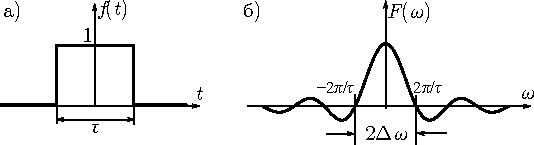
\includegraphics{Chapter_6/v6-single.pdf}
    \caption{Одиночный импульс (а) и его спектр (б)}
    \figmark{spectrum-one meander}
\end{figure}

Полезно сравнить спектр отдельного импульса со спектром периодической
последовательности одинаковых импульсов (рис.~\figref{spectrum-meander}).
Вместо \important{дискретного} спектра $\{c_n\}$ мы получили
\important{непрерывный} спектр~$C(\omega)$, причём
спектр импульса $C(\omega)$ (с множителем $1/T$) представляет собой
<<огибающую>> частокола спектральных компонент $c_n$
периодической последовательности импульсов.

Заметим также, что, как видно из графика, основной вклад дают гармоники, частоты
которых заполняют интервал $|\Delta\omega|<2\pi/\tau$. Это~--- полуширина
главного максимума функции $\frac{\sin\omega\tau/2}{\omega\tau/2}$. Диапазон
частот $\Delta\omega$ можно назвать характерной \important{шириной спектра}
$C(\omega)$.
\end{lab:example}


\introsubsection{Соотношение неопределённостей}
\label{sec:indeterminacy}

При рассмотрении Примеров~\ref{example:square-zug} и~\ref{example:square},
мы получили замечательное соотношение, связывающее между собой
длительность~$\Delta t$ сигнала с шириной его спектра~$\Delta \omega$:
\begin{equation}
    \eqmark{indeterminacy relation}
    \Delta t \cdot \Delta\omega \sim 2\pi.
\end{equation}

Оказывается, это соотношение имеет универсальный характер.
Оно остаётся справедливым по порядку величины для произвольного сигнала $f(t)$.
% (соответствующую строгую теорему можно найти в курсах математического анализа).
Чем больше длительность сигнала~$\Delta t$ (либо больше интервал времени,
в течение которого происходит его заметное изменение), тем \'{у}же спектр
сигнала~$\Delta\omega$, и, наоборот, чем короче сигнал (или быстрее происходит
изменение сигнала), тем шире его спектр, т.\,е. требуется более широкий интервал
частот гармонических колебаний, образующих в сумме данный сигнал.
В этом состоит смысл формулы \eqref{indeterminacy relation},
которая называется \term{соотношением неопределённостей}.

В общем случае, если у сигнала есть какое-то характерное время~$\Delta t$,
в его спектре обязательно возникнет некоторый характерный масштаб
$\Delta \omega \sim 2\pi /\Delta t$. Например, рассмотрим ограниченную
последовательность периодических импульсов с полной длительностью~$t_0$,
периодом~$T\ll t_0$ и длительностью каждого импульса~$\tau\ll T$.
Сигнал и его спектр представлены на рис.~\figref{indeterm}
(он может быть без труда рассчитан из формулы \eqref{Fourier integral-coef}
с использованием результатов разобранных выше Примеров~\ref{example:RLC}
и~\ref{example:square-zug}). На спектре видно три характерных масштаба частоты:
наибольший масштаб~$\Delta \omega_{\tau} = 2\pi/\tau$ задаёт ширину всего спектра,
масштаб~$\Delta \omega_T = 2\pi / T$ есть расстояние между соседними
спектральными пиками, и наконец наименьший машстаб $\Delta \omega_0 = 2\pi /t_0$,
соответствующий наибольшему характерному времени~$t_0$,
определяет ширину каждого пика.

\begin{figure}[h!]
\centering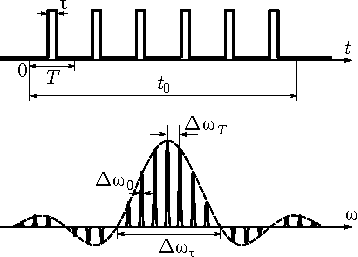
\includegraphics[scale=1.0]{Chapter_6/v6-indeterm.pdf}
\caption{Связь ширины спектра с характерными временными масштабами}
\figmark{indeterm}
\end{figure}

\introsubsection{Спектральный метод в задаче линейной фильтрации}

Сформулируем ещё раз алгоритм решения задачи линейной фильтрации
спектральным методом (методом Фурье) с учётом полученных соотношений.

Для нахождения отклика линейной системы $g(t)$ на воздействие $f(t)$
нужно:
\begin{enumerate}
    \item представить входной сигнал $f(t)$ в виде ряда
    \eqref{Fourier series} или интеграла Фурье \eqref{Fourier integral},
где спектр $\hat{\mathcal{F}}[f]$ (функция $C(\omega)$ или набор $\{c_n\}$)
находится с помощью соотношений \eqref{fourier-coeff}
или~\eqref{Fourier integral-coef};

    \item найти частотную характеристику фильтра
$\lambda(\omega)$, т.\,е. функцию отклика фильтра на гармоническое внешнее воздействие
единичной амплитуды:
\begin{equation*}
    e^{i\omega t}\to\fbox{$\hat\Lambda$}\to \lambda(\omega)e^{i\omega t};
\end{equation*}

    \item просуммировать отклики на каждое гармоническое
    слагаемое входного сигнала, что даёт спектр выходного сигнала:
    \begin{equation*}
    \sum c_n e^{i\omega_n t} \to\fbox{$\hat\Lambda$}\to \sum \lambda(\omega_n)c_n e^{i\omega_n t},
    \end{equation*}
    или
    \begin{equation*}
    \int C(\omega) e^{i\omega t} \to\fbox{$\hat\Lambda$}\to
    \int \lambda(\omega)\cdot C(\omega)e^{i\omega t};
    \end{equation*}
    \item восстановить выходной сигнал $g(t)$ по его спектру
    (обратное преобразование Фурье).
\end{enumerate}
Всю схему можно записать кратко одной формулой:
    \begin{equation}
        \eqmark{linear-filter-fourier}
    g(t) = \hat{\mathcal{F}}^{-1}\!
    \left[\lambda(\omega)\cdot \hat{\mathcal{F}}[f(t)]\right].
    \end{equation}


\begin{wrapfigure}[14]{o}{0.25\textwidth}
     \centering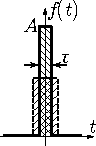
\includegraphics{Chapter_6/v6-delta.pdf}
     \caption{\footnotesize Предельный переход к дельта-импульсу}
\end{wrapfigure}

\begin{lab:example}\label{example:delta}
Устремим длительность импульса из предыдущего примера к нулю $\tau\to 0$,
при этом его амплитуду $A$ будем наращивать так, чтобы площадь
под его графиком оставалась постоянной (единичной): $\int f(t) = A \tau = 1$.
Такой импульс физике обозначают как $\delta(t)$ и называют \important{дельта-импульсом}
(или \important{дельта-функцией}).

Поскольку $\sin x/x\to 1$ при $x\to 0$,
предельный переход \eqref{spectrum-impulse} даёт простой результат:
\begin{equation}
    \eqmark{spectrum-delta}
    C(\omega)\to A\tau =1.
\end{equation}
То есть спектр бесконечно узкого импульса единичной площади (дельта-функции)
есть единичная константа. Заметим, что и здесь выполняется соотношение
неопределённостей: бесконечно узкий импульс даёт бесконечно широкий спектр.

Этот результат позволяет придать новый смысл частотной характеристике
(функции отклика) $\lambda(\omega)$ некоторого фильтра.
Если спектр входного сигнала $f(t)$ есть единичная константа,
то как следует из соотношения \eqref{linear-filter-fourier},
откликом системы будет функция $g(t)$, спектр которой совпадает
с $\lambda(\omega)$. Таким образом, \important{обратное преобразование Фурье
от функции отклика системы есть её реакция на единичный дельта-имульс}.
\end{lab:example}


\introsubsection{Физический смысл спектрального разложения}
\label{sec:spectrum-meaning}

Разложение функции $f(t)$ в ряд или интеграл Фурье может показаться
абстрактной математической операцией --- некоторым трюком, не имеющим
под собой физического содержания. Попробуем ответить на вопрос,
можно ли \important{измерить} амплитуды спектральных компонент $f(t)$,
тем самым приписав им прозрачный физический смысл.

Рассмотрим колебательный $RLC$-контур и подадим на его вход некоторый сигнал $f(t)$.
Для простоты ограничимся периодической функцией.

Пусть собственная частота контура равна $\Omega$, а добротность его
достаточно велика: $Q=\Omega/2\gamma \gg 1$ ($\gamma$ --- коэффициент затухания).

Пусть известно спектральное разложение $f(t)=\sum c_n e^{i\omega_n t}$.
После <<фильтрации>> через контур на выходе получим сигнал со
спектральными компонентами $g(t)=\sum g_n e^{i\omega_n t}$,
где $g_n = \lambda(\omega_n) c_n$ для каждого $n$,
$\lambda(\omega)$ --- частотная характеристика $RLC$-контура, найденная
выше (см. Пример~\ref{example:RLC}). Нетрудно видеть, что такое преобразование резко
(примерно в $Q$ раз) усиливает частоты входного сигнала, близкие к
$\Omega$ (т.\,е. к \important{резонансу}), и ослабляет далёкие.
В~пределе идеального контура ($Q\to \infty$), в спектре сигнала на выходе
останется единственная~--- резонансная~--- частота.
Сигнал $g(t)$ будет гармоническим колебанием с частотой $\Omega$:
$g(t) \propto c(\Omega) e^{i\Omega t}$,
причём его амплитуда будет пропорциональна амплитуде гармоники с этой
частотой в разложении исходной функции $f(t)$ (а если в этом разложении не было
гармоники $\omega_n=\Omega$, результирующая амплитуда будет нулевой).

Мы видим, что высокодобротный колебательный контур <<отфильтровывает>> из подаваемого
на него сигнала те спектральные компоненты, частоты которых близки к
его собственной $\Omega$. По амплитуде отклика можно измерить и амплитуду
гармоники в исходном сигнале. Меняя собственную частоту контура $\Omega$
(например, изменяя ёмкость конденсатора), можно в принципе просканировать весь
диапазон частот, измерив таким образом амплитуды всех спектральных
компонент~$c_n$ в разложении $f(t)=\sum c_n e^{i\omega_n t}$. Итак,
спектр сигнала может быть измерен непосредственно и описанная схема измерения
позволяет придать спектральному разложению наглядный физический смысл.

\begin{lab:example}\label{example:zug-RLC}
Рассмотрим колебательный $RLC$-контур с собственной
частотой~$\Omega$ и добротностью $Q\gg 1$, в котором мы попытаемся раскачать колебания,
подавая на вход периодическую последовательность коротких импульсов
с периодом $T$ и длительностью $\tau$. Можно ли раскачать колебания в контуре
до сколь-нибудь значимых амплитуд, если частота повторения импульсов
$\omega_0=2\pi/T$ много меньше резонасной частоты контура $\Omega$,
$\omega_0\ll \Omega$?

\begin{figure}[h!]
 \centering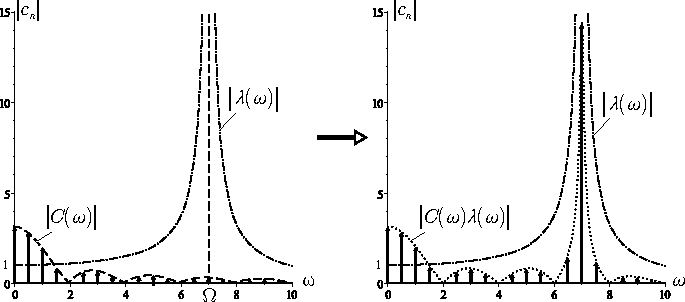
\includegraphics[width=\textwidth]{Chapter_6/v6-impulse-filter.pdf}
 \caption{\footnotesize Изменение спектра периодической последовательности импульсов (слева)
 в результате фильтрации колебательным контуром (справа) при резонансе с одной
 из высокочастотных гармоник. Расчёт проведён
 для $Q=50$, $\omega_0=\Omega/7$, $\tau=T/4$}
 \figmark{impulse-filter}
\end{figure}

Для нахождения амплитуды результирующих колебаний нужно перемножить
спектр периодической последовательности $\{c_n\}$
(см. Пример~\ref{example:square-zug}, \eqref{impulses-spectrum})
и частотную характеристику колебательного контура $\lambda(\omega)$
(см. Пример~\ref{example:RLC}, \eqref{RLC-lambda}).
Возможный результат такого преобразования представлен на рис.~\figref{impulse-filter}.
Видно, что благодаря существованию в спектре входного сигнала высокочастотных
гармоник $\omega_n = n \omega_0$, при выполнении условия
$\Omega = n \omega_0$, где $n$ --- целое, и при достаточно высокой добротности,
такая раскачка колебаний возможна.

Из \eqref{impulses-spectrum} видно, что амплитуды гармоник $|c_n|$ убывают
с ростом $n$ как $1/n$. С другой стороны, из \eqref{RLC-lambda} можно получить,
что в резонансе сигнал усиливается в $Q$ раз.
Таким образом, раскачать колебания в высокодобротном $RLC$-контуре можно
с помощью периодических импульсов, частота повторения $\omega_0=2\pi/T$
которых может быть существенно меньше резонансной,
вплоть до $\omega_0 \sim \Omega / Q \ll \Omega $.
\end{lab:example}

\introsubsection[Свойства преобразования Фурье]{%
    Свойства преобразования Фурье}
% \protect\footnote{При первом чтении данный раздел можно пропустить.}}

Рассмотрим некоторые свойства спектрального разложения (преобразования Фурье),
которые могут быть полезны при расчёте спектров.

\begin{wrapfigure}{o}{0.3\textwidth}
 \centering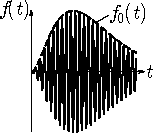
\includegraphics{Chapter_6/v6-modul.pdf}
 \caption{}
 \figmark{modul}
\end{wrapfigure}

\paragraph{Спектр огибающей, заполненной высокочастотным сигналом.}
Пусть $C_0(\omega)$ --- спектр некоторой функции $f_0(t)$.
Найдём спектр $C(\omega)$ функции
\begin{equation*}
f(t)=f_0(t)\cos(\omega_0 t).
\end{equation*}
Здесь $f_0(t)$ имеет смысл <<огибающей>>, заполненной колебаниями
с частотой~$\omega_0$ (см. рис.~\figref{modul}).

Используя формулу Эйлера \eqref{euler}, запишем
\begin{equation*}
    f(t)=\frac{1}{2}f_0(t)e^{i\omega_0t}+\frac{1}{2}f_0(t)e^{-i\omega_0t}.
\end{equation*}
Пользуясь \eqref{Fourier integral-coef}, найдём спектр
функции $f_0(t)e^{i\omega_0 t}$:
\begin{equation}
    \eqmark{task-spectrum-shift}
%     \int\limits_{-\infty}^\infty f_0(t)e^{i\omega_0 t}\cdot e^{-i\omega
% t}\,dt=
    \hat{\mathcal{F}}[f_0(t)e^{i\omega_0 t}]=
\int\limits_{-\infty}^\infty
f_0(t)e^{-i(\omega-\omega_0)t}\,dt=C_0(\omega-\omega_0),
\end{equation}
т.~е. при умножении на $e^{i\omega_0 t}$ исходный спектр
\important{сдвигается} по оси частот на величину $\omega_0$
(рис.~\figref{task-shift-spectrum}).

\begin{figure}[h!]
\centering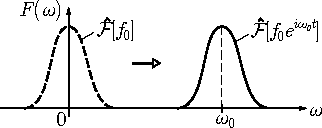
\includegraphics{Chapter_6/v6-shift.pdf}
\caption{Смещение спектра при домножении сигнала на $e^{i\omega_0 t}$}
\figmark{task-shift-spectrum}
\end{figure}

%\begin{equation}
%   \eqmark{task-freq-shift}
%   C(\omega)=e^{-i\omega\tau}\int_{-\infty}^\infty f_0(t')e^{-i\omega
% t'}\,dt'=C_0(\omega)\cdot e^{-i\omega\tau},
%\end{equation}
%или символически $f_0(t-\tau) \leftrightarrow C_0(\omega)e^{-i\omega\tau}$,
% т.е. смещение сигнала во времени на $\tau$ (запаздывание) приводит к умножению
% его спектра на $e^{-i\omega\tau}$ (теорема смещения).
%

Отсюда находим искомый спектр:
\begin{equation}
    \eqmark{task-2shift-spectrum-cos}
    C(\omega)=\frac{1}{2}C_0(\omega-\omega_0)+\frac{1}{2}C_0(\omega+\omega_0).
\end{equation}
Если частота $\omega_0$ существенно превосходит характерную ширину $\Delta \omega$
спектра огибающей, $\omega_0 \gg \Delta \omega$, то слагаемые
\eqref{task-2shift-spectrum-cos} не накладываются друг на друга.
Тогда искомый спектр $C(\omega)$ получается из $C_0(\omega)$
простым смещением по оси частот влево и вправо на <<несущую>>
частоту $\omega_0$ (с домножением на 1/2, см. рис.~\figref{task-2shift-spectrum-cos}).

\begin{figure}[h!]
%     \psfragfig[width=0.8\textwidth]{Images/Chapter_6/15b}{%
%     \psfrag{x}{$\omega$}
%     \psfrag{y}{$C_0(\omega)$}
%     \psfrag{z}{$C(\omega)$}
%     \psfrag{a}[ct]{$-\omega_0$}
%     \psfrag{b}[ct]{$\omega_0$}}
\centering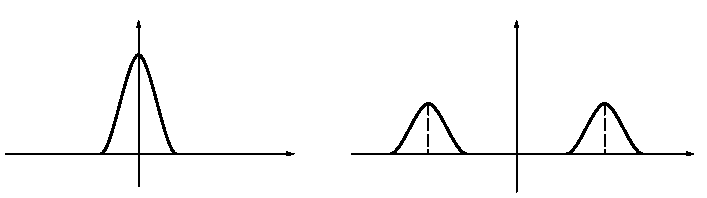
\includegraphics[width=0.8\textwidth]{Chapter_6/15b.pdf}
    \caption{Преобразование спектра при домножении на $\cos \omega_0 t$}
    \figmark{task-2shift-spectrum-cos}
\end{figure}

\begin{wrapfigure}{o}{0.5\textwidth}
%     \psfragfig[width=0.5\textwidth]{Images/Chapter_6/16}{%
%     \psfrag{t}{$t$}
%     \psfrag{f}{$f_0(t)$}
%     \psfrag{F}{$f(t)$}
%     \psfrag{a}[ct]{$\llap{$-$}\frac{\tau}{2}$}
%     \psfrag{b}[ct]{$\frac{\tau}{2}$}
%     \psfrag{A}{а)}
%     \psfrag{B}{б)}}
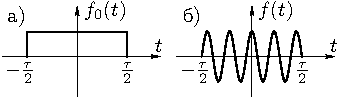
\includegraphics[width=0.5\textwidth]{Chapter_6/16}
    \caption{\footnotesize Прямоугольный импульс (а), ограничивающий синусоиду (б)}
    \figmark{one-zug}
\end{wrapfigure}

\begin{lab:example}\label{example:one-zug}
Найдём спектр обрывка синусоиды с частотой $\omega_0$
длительностью $\tau$ (такой сигнал называют \term{цугом}).
Сигнал может быть представлен как
\begin{equation*}f(t)=f_0(t)\cos(\omega_0 t),\end{equation*} где $f_0(t)$ --- единичный прямоугольный
импульс длительностью $\tau$ (см. рис.~\figref{one-zug}).

Пользуясь полученными ранее формулами для спектра прямоугольного импульса
\eqref{spectrum-impulse} и для смещения спектра \eqref{task-2shift-spectrum-cos},
получим
\begin{equation*}
C(\omega)=\frac{\tau}{2}\left[\frac{\sin(\omega-\omega_0)\tau/2}{
(\omega-\omega_0)\tau/2}+
\frac{\sin(\omega+\omega_0)\tau/2}{(\omega+\omega_0)\tau/2}
\right].
\end{equation*}
Спектры $C_0(\omega)$ и $C(\omega)$ представлены на
рис.~\figref{task-meander-train-spectrum}.

\begin{figure}[h!]
%     \psfragfig[width=0.8\textwidth]{Images/Chapter_6/17}{%
%     \psfrag{p}[br]{$\tau$}
%     \psfrag{q}{$\tau/2$}
%     \psfrag{w}{$\omega$}
%     \psfrag{f}{$C_0(\omega)$}
%     \psfrag{F}{$C(\omega)$}
%     \psfrag{a}[ct]{$\llap{$-$}\omega_0$}
%     \psfrag{b}[ct]{$\omega_0$}
%     \psfrag{A}{а)}
%     \psfrag{B}{б)}}
\centering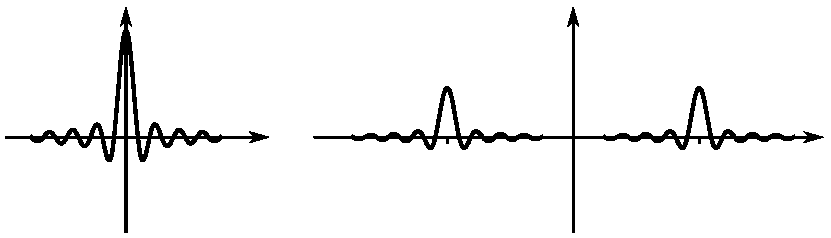
\includegraphics[width=0.8\textwidth]{Chapter_6/17}
    \caption{Спектры а) прямоугольного импульса, б) импульса,
        заполненного синусоидой (цуга)}
    \figmark{task-meander-train-spectrum}
\end{figure}
\end{lab:example}


\begin{lab:example}\label{example:exp}
Найдём спектр затухающих колебаний
\begin{equation*}
f(t) = e^{-\gamma t} \sin \omega_0 t\qquad (\text{при~}t\ge 0).
\end{equation*}
По формуле \eqref{Fourier integral-coef} находим спектр затухающей
экспоненты (начинающейся с $t=0$):
\begin{equation*}
\hat{\mathcal{F}}[e^{-\gamma t}] =
\int\limits_0^{\infty} e^{-\gamma t - i\omega} dt =
\frac{1}{\gamma + i\omega}
\end{equation*}
(ср. с Примером~\ref{example:RC}).
Пользуясь формулой Эйлера для синуса
\begin{equation*}
\sin \alpha = \frac{e^{i\alpha} - e^{-i\alpha}}{2i},
\end{equation*}
получим искомый спектр по формуле смещения \eqref{task-spectrum-shift}:
\begin{equation*}
C(\omega) = \frac{1}{2i} \left[\frac{1}{\gamma + i(\omega-\omega_0)} -
\frac{1}{\gamma + i(\omega+\omega_0)}\right] =
\frac{\omega_0}{\omega_0^2 + \gamma^2 - \omega^2 +2i\gamma \omega }.
\end{equation*}

Обратим внимание, что если положить $\omega_0^2 =\Omega^2 - \gamma^2$,
полученный ответ совпадает (с точностью до константы)
с частотной характеристикой колебательного контура \eqref{RLC-lambda}.
Это не удивительно, поскольку именно затухающие колебания
$f(t) = e^{-\gamma t} \sin \omega_0 t$
возникают в колебательном контуре, если сообщить ему единичный дельта-импульс
(см. также Пример~\ref{example:delta}).
\end{lab:example}

\paragraph{Упражнение.} Предлагаем читателю самостоятельно получить
спектр периодической последовательности цугов (см. рис.~\figref{zug-zug}).

% FIXME: Figure missing!
\begin{figure}[h!]
\hfil
    \oldpic{0.5\textwidth}{Chapter_6/v6-zug}
    \caption{Периодическая последовательность цугов}
    \figmark{zug-zug}
\end{figure}

\paragraph{Теорема смещения.}
Найдём спектр $C(\omega)$ сигнала, смещённого по времени: $f(t)=f_0(t-\tau)$,
где $f_0(t)$ --- функция с известным спектром~$C_0(\omega)=\hat{\mathcal{F}}[f_0]$.

По определению имеем
\begin{equation*}
  C(\omega)=\hat{\mathcal{F}}[f(t)]=\int\limits_{-\infty}^\infty f_0(t-\tau)e^{-i\omega t}\,dt.
\end{equation*}
После замены переменных $t'=t-\tau$ ($dt=dt'$) получаем
\begin{equation*}
  C(\omega)=\int\limits_{-\infty}^\infty f_0(t') e^{-i\omega(t'+\tau)}\,dt'.
\end{equation*}
Множитель $e^{-i\omega\tau}$ (не зависящий от переменной интегрирования $t'$)
выносится из-под знака интеграла:
\begin{equation}
  \eqmark{task-freq-shift}
  C(\omega)=e^{-i\omega\tau}\int\limits_{-\infty}^\infty f_0(t')e^{-i\omega
t'}\,dt'= e^{-i\omega\tau} \cdot C_0(\omega),
\end{equation}
или символически
\begin{equation*}
\hat{\mathcal{F}}[f_0(t-\tau)] = e^{-i\omega\tau} \hat{\mathcal{F}}[f_0(t)],
\end{equation*}
т.\,е. смещение сигнала во времени на $\tau$ (запаздывание)
приводит к умножению его спектра на $e^{-i\omega\tau}$ (\term{теорема смещения}).

Заметим, что поскольку $|e^{-i\omega t}|=1$, смещение по времени не меняет
амплитуд спектральных компонент, а лишь сдвигает их фазы (пропорционально частоте
компоненты).

\paragraph{Спектр произведения сигналов.}
Пусть $F(\omega)=\hat{\mathcal{F}}[f(t)]$ --- спектр функции $f(t)$, а
$G(\omega)=\hat{\mathcal{F}}[g(t)]$ ---
спектр функции $g(t)$. Найдём спектр $H(\omega)=\hat{\mathcal{F}}[fg]$
произведения $h(t)=f(t)\cdot g(t)$.

Воспользуемся разложением функции на гармоники в форме
интеграла Фурье~\eqref{Fourier integral}:
\begin{equation*}
f(t) = \frac{1}{2\pi} \int\limits_{-\infty}^{\infty} F(\omega)e^{i\omega t} d\omega
\end{equation*}
Согласно \eqref{Fourier integral-coef} искомый спектр равен
\begin{equation*}
H(\omega) = \int\limits_{-\infty}^{\infty} f(t) g(t) e^{-i\omega t} dt =
\frac{1}{2\pi} \int\limits_{-\infty}^{\infty} dt
\int\limits_{-\infty}^{\infty} d\omega' F(\omega') g(t) e^{-i(\omega-\omega')t}.
\end{equation*}
Меняя порядок интегрирования по $dt$ и $d\omega'$, получим искомую связь:
\begin{equation}
    \eqmark{folding}
H(\omega) = \int\limits_{-\infty}^{\infty} F(\omega')G(\omega-\omega') d\omega'.
\end{equation}
Интеграл в правой части называется \term{свёрткой}
функций~$F(\omega)$ и~$G(\omega)$. Таким образом, спектр произведения сигналов
равен свёртке их спектров.

% Свёртка \eqref{folding} означает, что при вычислении произведения сигналов~
% $f(t)\cdot g(t)$ каждая отдельная спектральная компонента~$f$
% взаимодействует со \important{всеми} спектральными компонентами~$g$,
% а результат их взаимодействия суммируется.

Свертку функций часто обозначают как $F * G$. Тогда можно сокращённо записать
\begin{equation*}
 \hat{\mathcal{F}}[f\cdot g] = \hat{\mathcal{F}}[f] * \hat{\mathcal{F}}[g].
\end{equation*}

Аналогичным образом нетрудно доказать <<обратную>> теорему:
спектр свёртки $f*g = \int f(\tau) g(t-\tau) d\tau$ равен произведению
спектров~$f(t)$ и~$g(t)$:
\begin{equation*}
\hat{\mathcal{F}}[f*g] = \hat{\mathcal{F}}[f] \cdot \hat{\mathcal{F}}[g].
\end{equation*}

\paragraph{Связь спектра с энергией. Теорема Парсеваля.}
Если $C(\omega)$ --- спектр функции $f(t)$, для них справедливо следующее
соотношение, называемое \term{равенством Парсеваля}:
\begin{equation}
    \eqmark{parseval-int}
\int\limits_{-\infty}^{\infty} |f(t)|^2 dt =
\int\limits_{-\infty}^{\infty} |C(\omega)|^2 d\omega
\end{equation}
или, если функция $f(t)$ периодическая со спектром $\{c_n\}$, то
\begin{equation}
    \eqmark{parseval-dicrete}
\frac{1}{T}\int\limits_{0}^{T} |f(t)|^2 dt =
\sum\limits_n |c_n|^2.
\end{equation}

Поскольку квадрат сигнала $|f(t)|^2$, как правило, пропорционален
его~\important{мощности}, это соотношение имеет важное значение для физики.
Оно показывает, что \important{полная энергия сигнала за период
пропорциональна сумме интенсивностей} (т.\,е. квадратов модулей $|c_n|^2$)
\important{всех его спектральных компонент}.

Получим равенство \eqref{parseval-dicrete} для случая дискретного спектра
периодической функции. За доказательством общего случая отсылаем
к специализированной литературе. Домножим разложение
\eqref{Fourier-periodic osc} функции $f(t)$ по гармоникам на комплексно
сопряжённое ему:
\begin{equation*}f(t)f^{\star}(t) = \sum\limits_n c_n e^{i n \omega_0 t} \cdot \sum\limits_k c_k^{\star} e^{-i k \omega_0 t}.\end{equation*}
В~результате получится сумма, содержащая слагаемые вида
$c_n c_k^{\star} e^{i(n-k)\omega_0 t}$ для всех возможных пар целых~$n$ и~$k$.
Итеграл по отрезку $t\in[0,T]$ от фукнций $e^{i(n-k)\omega_0 t}$
обращается в нуль, если $n\ne k$, и равен $T$, если $n=k$.
С учётом того, что $f(t)f^{\star}(t) = |f(t)|^2$ и
$c_n c_n^{\star} = |c_n|^2$, получаем окончательно формулу
\eqref{parseval-dicrete}.



\introsection{Модуляция}

Для передачи сигналов~--- музыки, речи, телевизионного изображения~---
необходимо нарушение синусоидальности. Отклонение
от синусоидальности и выражает содержание передаваемой информации. Колебательный
процесс, отличный от гармонического,
назовём \term{модулированным колебанием}. Примеры таких процессов (их
осциллограммы) приведены на рис.~\figref{modulated oscillation}.

\begin{figure}[h!]
    \includegraphics[width=\textwidth]{Chapter_6/5.pdf}
    \caption{Примеры модулированных колебаний: а,~б)~--- по амплитуде,
    в)~--- по фазе (частоте)}
    \figmark{modulated oscillation}
\end{figure}

Будем записывать модулированные колебания в виде
\begin{equation}
    \eqmark{modulated oscillation}
    f(t)=a(t)\cos(\omega_0t+\varphi(t)).
\end{equation}
В отличие от гармонического колебания, здесь $a(t)$ и $\varphi(t)$~---
меняющиеся во времени величины. Форма записи \eqref{modulated oscillation}
особенно целесообразна в том случае, когда $a(t)$ и $\varphi(t)$~---
\important{медленно} меняющиеся функции времени, т.\,е.
эти функции остаются практически неизменными --- $a(t)\approx a_{0}$ и
$\varphi(t)\approx\varphi_0$ --- на интервалах времени~$\tau$,
существенно превышающих период гармонического (\term{несущего})
колебания частоты $\omega_0$:
\begin{equation}
    \eqmark{quasiharmonic oscillation - tau}
    \tau \gg \frac{2\pi}{\omega_0}.
\end{equation}
Такое колебание называется \term{квазигармоническим}.
В этом случае медленно меняющиеся величины~$a(t)$ и~$\varphi(t)$
принято называть \important{амплитудой} и \important{начальной фазой} модулированного колебания
соответственно.

Итак, квазигармоническое колебание можно характеризовать двумя параметрами:
периодом несущего колебания $T_0=2\pi/\omega_0$ и временем $\tau \gg T_0$,
характеризующим быстроту изменения амплитуды $a(t)$ и (или) начальной
фазы $\varphi(t)$.

Для описания модулированных колебаний используется
следующая терминология: говорят, что функция $a(t)$ описывает закон амплитудной
модуляции, а функция $\varphi(t)$~--- закон
фазовой модуляции. Именно в этих функциях и может быть заложена
передаваемая информация.

Если $\varphi(t)=\varphi_0=\const$, то
\begin{equation}
    \eqmark{amplitude-modulated}
    f(t)=a(t)\cos(\omega_0t+\varphi_0),
\end{equation}
где $a(t)\ge0$. Такое колебание называют
\term{модулированным по амплитуде}.

Если $a(t)=a_0=\const$, то
\begin{equation}
    \eqmark{phase-modulated}
    f(t)=a_0 \cos(\omega_0t+\varphi(t)).
\end{equation}
Такое колебание называют \term{модулированным по фазе}.%
\footnote{Иногда выделяют также \term{частотную модуляцию}:
    \begin{equation*}
     f(t)=a_0 \cos\left(\int\omega(t) dt\right).
    \end{equation*}
Заменой $\omega(t) = \omega_0 + \frac{d\varphi}{dt}$ она сводится
к фазовой.}

Осциллограммы процессов на рис. \figref{modulated oscillation}а, б являются
примерами амплиту\-дно-модулированных колебаний, а на
рис.~\figref{modulated oscillation}в~--- пример колебания, модулированного по фазе.

\introsubsection{Спектры модулированных сигналов}\label{sec:modulated-spectrum}
\paragraph{Амплитудная модуляция.}
Рассмотрим простейшее амплитудно-модулированное колебание, в котором
амплитуда модуляции является гармонической функцией:
\begin{equation}
    \eqmark{example-amplitude-modulated}
    f(t)=a(t)\cos\omega_0t,\qquad \text{где~}a(t)=a_0(1+m\cos\Omega t).
\end{equation}
Константа $0<m\le 1$ называется \term{глубиной модуляции}.
Глубину модуляции можно выразить через максимальную $a_{\rm max}$ и
минимальную $a_{\rm min}$
амплитуды сигнала:
\begin{equation}
    \eqmark{modul-deep}
    m = \frac{a_{\rm max} - a_{\rm min}}{a_{\rm max} + a_{\rm min}}.
\end{equation}

Раскрывая скобки в \eqref{example-amplitude-modulated}
и пользуясь формулой для произведения косинусов, можно получить
\begin{equation}
    \centering
    \begin{aligned}
        f(t)=a_0(1+m\cos\Omega t)\cos\omega_0t=&\\
=a_0\cos\omega_0t+\frac{ma_0}{2}\cos(\omega_0+\Omega)t+
\frac{ma_0}{2}\cos&(\omega_0-\Omega)t.
    \end{aligned}
    \eqmark{ex-amplitude-modulated-sum}
\end{equation}

Итак, амплитудно-модулированное колебание с законом модуляции
\eqref{example-amplitude-modulated} представляется в виде суммы трёх
гармонических колебаний (трёх гармоник):
\begin{equation*}
    f_{0}(t)=a_0\cos\omega_0t,\quad
f_1(t)=\frac{ma_0}{2}\cos(\omega_0+\Omega)t,\quad
    f_2(t)=\frac{ma_0}{2}\cos(\omega_0-\Omega)t
\end{equation*}
с частотами соответственно $\omega_0$, $\omega_0+\Omega$, $\omega_0-\Omega$ и
амплитудами $a_0$, $ma_0/2$,
$ma_0/2$. Колебание $f_0(t)$ называется \term{несущим колебанием}, а
$f_1(t)$ и $f_2(t)$~--- \term{боковыми
гармониками}. Условие квазигармоничности колебания $f(t)$: $\Omega\ll\omega_0$.

\paragraph{Фазовая модуляция.}
Рассмотрим теперь простейший пример фазовой модуляции:
\begin{equation}
    \eqmark{example-phase-modulated}
    f(t)=a_0\cos(\omega_0t+\varphi(t)),\qquad \text{где}\quad
\varphi(t)=m\cos\Omega t.
\end{equation}
Константа $m$~--- \term{глубина модуляции фазы}~--- определяет диапазон
изменения начальной фазы (от $-m$ до $+m$).

Раскрывая косинус суммы, запишем $f(t)$ в виде
\begin{equation*}
    f(t)=a_0\bigl(\cos\omega_0t\cos\varphi(t)-\sin\omega_0t\sin\varphi(t)\bigr).
\end{equation*}

В общем случае закон модуляции \eqref{example-phase-modulated} приводит к
довольно сложному спектру (с большим числом слагаемых гармонических
колебаний). Мы рассмотрим случай $m\ll 1$ (малая глубина модуляции фазы),
когда можно использовать приближённые
выражения: $\cos\varphi(t)\approx 1$ и $\sin\varphi(t)\approx\varphi(t)$
(мы отбрасываем величины порядка $m^2$ и выше). Тогда
\begin{equation*}
    f(t)=a_0\cos\omega_0t-a_0 m\sin\omega_0t\cos\Omega t,
\end{equation*}
или (т.~к. $2\sin\alpha\cos\beta=\sin(\alpha+\beta)+\sin(\alpha-\beta)$):
\begin{multline}
    \eqmark{ex-phase-modulated-sum}
f(t)=a_0\cos\omega_0t+\frac{ma_0}{2}\cos
\left((\omega_0+\Omega)t+\frac{\pi}{2}\right)+\\
+\frac{ma_0}{2}\cos\left((\omega_0-\Omega)t+\frac{\pi}{2}\right).
\end{multline}
Это и есть искомое представление колебания $f(t)$ в виде суммы гармонических
колебаний.

\todo[inline]{Добавить на график значения боковых частот}

\begin{figure}[h]
%     \psfragfig[width=0.5\textwidth]{Images/Chapter_6/10}{%
%     \psfrag{a}[ct]{$\omega_0$}
%     \psfrag{b}[ct]{$-\omega_0$}
%     \psfrag{c}[ct]{$\omega_0-\Omega$}
%     \psfrag{d}[ct]{$\omega_0+\Omega$}
%     \psfrag{o}[ct]{0}
%     \psfrag{1}{$a_0$}
%     \psfrag{2}{$\dfrac{ma_0}{2}$}
%     \psfrag{3}{$\dfrac{a_0}{2}$}
%     \psfrag{4}{$\dfrac{ma_0}{4}$}
%     \psfrag{x}[tl]{$\omega$}
%     \psfrag{y}{$a_n$}
%     \psfrag{z}{$c_n$}
%     \psfrag{A}{а)}
%     \psfrag{B}{б)}}
\centering
\includegraphics[width=0.35\textwidth]{Chapter_6/10}
    \caption{Спектр модулированных колебаний: действительное (вверху)
    и комплексное (внизу) представления}
    \figmark{spectrum-modulated}
\end{figure}

Сравним формулы \eqref{ex-amplitude-modulated-sum} и \eqref{ex-phase-modulated-sum}.
Первая из них~--- разложение в спектр колебания, модулированного по амплитуде,
вторая~--- колебания, модулированного по фазе. Эти колебания сильно различаются
по форме (сравните осциллограммы на рис.~\figref{modulated oscillation}б
и \figref{modulated oscillation}в), однако их спектры весьма похожи
(см. рис.~\figref{spectrum-modulated}). В обоих случаях в правой части три
слагаемых, три гармонических колебания, имеющих одинаковые частоты ($\omega_0$,
$\omega_0\pm\Omega$) и амплитуды ($a_0$~--- несущие колебания, $ma_0/2$~---
боковые гармоники). Различие выглядит небольшим: боковые гармоники отличаются
фазовым сдвигом $\frac{\pi}{2}$. Однако это различие приводит к кардинальному
отличию в форме (в осциллограмме $f(t)$) результирующего сигнала.

Приведённый пример показывает, для восстановления сигнала $f(t)$ по его спектру важно
знать \important{не только амплитуды} спектральных компонент, \important{но и их фазы}
(это важно, поскольку на практике фазы измерять сложнее, и информация о
них часто бывает утеряна).


\introsubsection{Детектирование модулированных сигналов}

Процедуру, обратную модуляции, называют \term{детектированием}.
При получении модулированного (по фазе или амплитуде) сигнала необходимо
выделить из него информацию, содержащуюся в функциях $a(t)$ или
$\varphi(t)$, отбросив по возможности высокочастотное колебание
на несущей частоте $\omega_0$ (не несущее информации).

Весь спектр модулированного сигнала сосредоточен в узкой области
вблизи большой несущей частоты $\omega_0\pm \Omega$, где $\Omega$ ---
характерная частота модуляции. Необходимо преобразовать сигнал так,
чтобы полезная информация оказалась в области низких частот. Это можно
сделать \important{нелинейными} элементами. Одним из простейших способов
детектирования является использование элементов с квадратичным законом связи
(\term{квадратичное детектирование}) между входным и выходным сигналом:
$g(t)\propto f^2(t)$ (другой способ --- использование \term{выпрямляющих}
преобразователей, например, полупроводниковых диодов).

Для того, чтобы избавиться от <<ненужных>> (не содержащих полезную
информацию) высокочастотных составляющих можно применять обычные линейные
фильтры (см., в частности, Пример~\ref{example:RC}). Действие такого фильтра может быть сведено к усреднению во времени
сигнала по интервалу $\Delta t$, который существенно превосходит период
колебаний несущей, но значительно меньше периода колебаний <<информативных>>
функций $a(t)$ или $\varphi(t)$:
\begin{equation}
    \eqmark{averages-sq}
g(t) = \left<f^2(t)\right>_{\Delta t} = \frac{1}{\Delta t}
\int\limits_{t}^{t+\Delta t} f^2(t')\,dt',
\end{equation}
где
\begin{equation}
    \eqmark{averages-cond}
    \frac{2\pi}{\omega_0} \ll \Delta t \ll \frac{2\pi}{\Omega}.
\end{equation}
Схема квадратичного детектирования приведена на рис.~\figref{detect2}.
\begin{figure}[h]
 \includegraphics[width=\textwidth]{Chapter_6/v6-detect2.pdf}
 \caption{Схема детектирования модулированного сигнала:
     а) исходный сигнал $f(t)$, б) квадратичный сигнал
 $f^2(t)$, в) результат $g(t)$ усреднения по интервалу $\Delta t$.
Отличие $g(t)$ от $\frac12a^2(t)$ (отклонение и шум)
связаны с недостаточно хорошим выполнением сильного неравенства
\eqref{averages-cond}}
 \figmark{detect2}
\end{figure}

\paragraph{Квадратичное детектирование амплитудно-модулированного сигнала.}
Рассмотрим, как преобразование \eqref{averages-sq} действует на
амплитудно модулированный сигнал $f(t) = a(t) \cos \omega_0 t$. Имеем
\begin{equation*}
 g(t) = \left<f^2(t)\right>_{\Delta t} =
 \frac{1}{\Delta t}
\int\limits_{t}^{t+\Delta t} a^2 (t') \cos^2(\omega_0 t')\,dt'.
\end{equation*}
Ввиду соотношения \eqref{averages-cond} амплитуда~$a(t)$ практически не меняется
на отрезке $[t,\,t+\Delta t]$, поэтому её можно вынести из-под знака интеграла:
\begin{equation}
 g(t)= \frac{a^2(t)}{\Delta t} \int\limits_{t}^{t+\Delta t} \cos^2(\omega_0 t')\,dt'\approx
 \frac12 a^2(t).
\end{equation}
Последний переход справедлив, поскольку $\Delta t \gg 2\pi/\omega_0$ и
можно приближённо считать, что интегрирование ведётся по целому числу периодов
$2\pi /\omega_0$.
Таким образом, предложенная схема измеряет \important{квадрат амплитуды модуляции}.

Если имеет место модуляция гармонической функцией
\eqref{example-amplitude-modulated}
с малой глубиной модуляции $m\ll 1$, то
\begin{equation*}
 g(t) = \frac12 a_0^2 (1+m\cos\Omega t)^2 \approx
 \frac12 a_0^2 (1+2m\cos\Omega t).
\end{equation*}
Видно, что после квадратичного детектирования остаётся гармонический
сигнал $m a_0^2 \cos\Omega t$ на частоте модуляции, существующий на фоне
постоянного сигнала $a_0^2/2$.

\paragraph{Квадратичное детектирование фазово-модулированного сигнала.}
У сигнала, модулированного по фазе, амплитуда постоянна: $a(t)=\const$.
Можно ли в таком случае использовать квадратичное детектирование?

Как мы выяснили выше, спектры фазово- и амплитудно-модулированного сигналов
отличаются лишь начальными фазами гармоник. Изменив с помощью линейного фильтра
фазу несущего колебания (или боковых гармоник) на $\frac{\pi}{2}$,
мы можем преобразовать колебание, модулированное по фазе,
в амплитудно-модулированное колебание. Это известный в
радиотехнике \term{приём с изменением фазы несущей}.

Ещё один один метод --- \term{приём без несущей}, при котором из
спектра <<убирается>> (также линейным фильтром)
несущее колебание $a_0\cos\omega_0t$. Предлагаем читателю самостоятельно
проанализировать, что будет представлять собой результирующее колебание.

Аналогичные приёмы преобразования фазовой модуляции в амплитудную
применяются в оптике при наблюдении прозрачых структур ---
методы <<фазового контраста>> и <<тёмного поля>>.


\introsection{Синтез сигналов}\label{sec:synth}

Возможность разложить произвольную функцию $f(t)$ в ряд (или интеграл)
Фурье единственным и однозначным способом подразумевает и возможность
<<собрать>> сигнал любой формы, используя гармонические колебания с подобранными
амплитудами и фазами, совершив таким образом \important{обратное} преобразование Фурье.

Спектр реального сигнала в общем случае содержит бесконечное количество
гармоник, поэтому синтезировать исходный сигнал можно, как правило,
лишь в некотором приближении. Степень совпадения будет определяться
количеством синтезирующих гармоник (чем больше, тем лучше).

\begin{figure}[h!]
 \centering\includegraphics[scale=0.9]{Chapter_6/v6-meandr.pdf}
 \caption{Прямоугольный сигнал (меандр)}
 \figmark{meandr-delta}
\end{figure}

Рассмотрим в качестве примера прямоугольный сигнал, принимающий
значения $\pm 1$ со скважностью $\tau/T=1/2$ (<<меандр>>,
рис.~\figref{meandr-delta}). Из формулы \eqref{impulses-spectrum} имеем спектр
\begin{equation*}
c_n = \frac{\sin \pi n/2}{\pi n/2}.
% =
% \begin{cases}
%     0 & n\text{~--- чётное},\\
%     \frac{(-1)^{\frac{n-1}{2}}}{\pi n}& n\text{~--- нечётное}.
% \end{cases}
\end{equation*}
Переходя к амплитудам и фазам согласно \eqref{Fourier-coefficient},
найдём
\begin{equation*}
a_{2k}=0,\quad a_{2k-1} = \frac{4}{\pi (2k-1)},\quad
\varphi_{2k-1} = \pi (k-1),\qquad k=1,\,2,\,\ldots
\end{equation*}
($c_0=a_0=0$). Первые несколько слагаемых в спектральном разложении:
\begin{equation*}
f(t) \approx \frac{4}{\pi} \left[ \cos \omega_0 t -
\frac{1}{3}\cos 3\omega_0 t +
\frac{1}{5}\cos 5\omega_0 t -
\frac{1}{7}\cos 7\omega_0 t + \ldots\right]
\end{equation*}
На рис.~\figref{meandr-synthesis} представлен результат аппроксимации
рассматриваемой функции $k$ первыми слагаемыми её ряда Фурье.
Видно, что с увеличением числа слагаемых аппроксимация становится всё точнее.

При внимательном рассмотрении можно заметить интересную особенность:
колебания частичной суммы ряда особенно сильны около точек разрыва
функции $f(t)$. Причём
амплитуда первого максимума этих колебаний (в непосредственной близости от
разрыва) \important{не убывает} с ростом числа слагаемых (и составляет около 18\%
от величины скачка). Это явление получило название \term{явление Гиббса}.
Математически оно является следствием \important{неравномерной} сходимости ряда
Фурье разрывной функции. Если функция непрерывна и ограничена, то сходимость
её ряда Фурье будет равномерной (\important{признак Дирихле}) и подобных проблем
не возникает\footnote{См., например,
\important{Фихтенгольц Г.М.} Курс дифференциального и интегрального исчисления,
Т.~III, Гл.~19, \S4.}.

\begin{figure}[h!]
 \hfill\includegraphics{Chapter_6/v6-synthes.pdf}
 \caption{Аппроксимация разрывной функции частичными суммами ряда Фурье
 ($k$ --- число ненулевых слагаемых)}
\figmark{meandr-synthesis}
\end{figure}

С физической точки зрения по-настоящему \important{мгновенный} скачок функции
невозможен~--- всегда есть какое-то конечное (возможно, очень малое) время
перехода~$\delta\tau$. В таком случае явление Гиббса исчезнет, когда в
частичную сумму ряда Фурье попадут слагаемые, с помощью которых можно
<<разрешить>> столь малые масштабы по времени, то есть с частотами
порядка $\omega \sim 2\pi /\delta \tau$.

\begin{lab:questions}
\item Как можно измерить коэффициенты ряда Фурье (спектр) некоторого сигнала?

\item Изобразите схематично спектры $C(\omega)$:
\begin{itemize}
    \item бесконечно длинной синусоиды;
    \item синусоиды конечной длины;
    \item периодической последовательности прямоугольных импульсов;
    \item одного прямоугольного импульса.
    \item периодической последовательности цугов;
    \item одного цуга.
\end{itemize}

\item Чем отличаются спектры амплитудно- и фазово-модулированного сигналов?

\item Как изменится спектр периодической последовательности
прямоугольных импульсов, если убрать каждый второй импульс?

\item Как изменится спектр периодической последовательности прямоугольных
импульсов, если уменьшить длительность каждого импульса в два раза?

\item Что такое детектирование? Какие существуют методы детектирования
фазово-модулированного сигнала?

\item Предложите электрическую схему низкочастотного линейного фильтра.

\item Периодический прямоугольный сигнал подали на интегрирующую $RC$-цепочку
(рис.~\figref{RC}). Как в результате изменится форма сигнала?

\end{lab:questions}

\begin{lab:literature}
    \item \textit{Сивухин~Д.В.} Общий курс физики.~Т.III. Электричество ---
М.:~Физматлит, 2003.~--- \S~128.
    \item \textit{Кингсеп~А.С., Локшин~Г.Р., Ольхов~О.А.} Основы физики.~Т.I.---
М.:~Физматлит, 2007.~--- Гл I, \S\S~1.5, 1.6.
    \item \textit{Кириченко Н.А.} Электричество и магнетизм: учебн. пособие.---
    М.:~МФТИ, 2011.~--- \S\S~17.4--17.7.
    \item \textit{Локшин~Г.Р., Козел~С.М.} Модулированные колебания. Спектральный
анализ. Линейная фильтрация --- М.:~МФТИ, 2009.
\item *\textit{Булыгин В.С.} Явление Гиббса --- М.:~МФТИ, 2014.
\end{lab:literature}

% ---------------------------------------------




\lab{Спектральный анализ электрических сигналов}
\aim{изучить спектральный состав периодических электрических сигналов.}

\equip{анализатор спектра (аналоговый или цифровой),
    генератор прямоугольных импульсов и сигналов специальной формы, осциллограф.}

Перед выполнением работы необходимо ознакомиться с теоретическим введением
к разделу.

В работе изучается спектральный состав периодических электрических сигналов
различной формы: последовательности прямоугольных импульсов, последовательности
цугов и амплитудно-модулированных гармонических колебаний. Спектры этих сигналов
наблюдаются с помощью анализатора спектра и сравниваются c рассчитанными
теоретически.

Периодическая функция может быть представлена в виде бесконечного ряда
гармонических функций --- ряда Фурье (см. п.~\ref{sec:spectrum-periodic}
Введения):
\begin{equation*}
f(t) = \sum_{n=-\infty}^{\infty} c_n e^{in\omega_0 t}\qquad\text{или}\qquad
f=\sum_{n=0}^{\infty} a_n \cos (n\omega_0 t + \varphi_n).
\end{equation*}
Здесь $\omega_0 = 2\pi/T$, где $T$ --- период функции $f(t)$.
Коэффициенты $\{c_n\}$ могут быть найдены по формуле
\chaptereqref{fourier-coeff}:
\begin{equation*}
    c_n=\frac{1}{T}\int\limits_{0}^{T} f(t)e^{-in\omega_0 t}\,dt.
\end{equation*}
Наборы коэффициентов разложения в комплексной $\{c_n\}$ и действительной
$\{a_n,\varphi_n\}$ формах связаны соотношением \chaptereqref{Fourier-coefficient}:
\begin{equation*}
a_n = 2|c_n|,\qquad \varphi_n = \arg c_n.
\end{equation*}

\begin{wrapfigure}{o}{0.3\textwidth}
    \centering
    \includegraphics{Chapter_6/6-1-RLC.pdf}
    \caption{Колебательный контур как узкополосный фильтр}
    \figmark{simple-RLC}
\end{wrapfigure}

В качестве простейшего спектрального анализатора можно использовать
высокодобротный колебательный контур с подстраиваемой ёмкостью или
индуктивностью, рис.~\figref{simple-RLC}
(см. также п.~\ref{sec:spectrum-meaning} Введения).
Такой контур усиливает те гармоники входного сигнала $f(t)$,
частота которых близка к резонансной
$\nu_{рез} = 1/(2\pi\sqrt{LC})$, и практически не реагирует на частоты,
далёкие от $\nu_{рез}$. С точки зрения преобразования гармоник колебательный контур
является узкополосным \term{фильтром} с шириной полосы
пропускания порядка $\Delta \nu \sim \nu_{рез}/ Q$, где $Q =
\frac{1}{R}\sqrt{\frac{L}{C}} \gg 1$~--- его добротность. Амплитуда колебаний
в контуре пропорциональна амплитуде~$|c_n|$ гармоники $\nu_n=\nu_{рез}$
в фурье-спектре функции $f(t)$. Таким образом, меняя резонансную частоту контура,
можно <<просканировать>> весь спектр входного сигнала.

\experiment

У описанной выше схемы есть существенный недостаток: при изменении~$L$ или~$C$
меняется также и добротность, а значит и ширина полосы пропускания.
Кроме того, изготовление настраиваемых контуров с высокой добротностью
непрактично. В~связи с этим, как правило, для фильтрации сигнала
применяется другая схема.

Исследуемый сигнал $f(t)$ и сигнал от вспомогательного генератора гармонических
колебаний частоте~$\nu_{гет}$ (генератор в таких схемах называют
\term{гетеродином}) подаются на вход \term{смесителя}. Смеситель
представляет собой нелинейный элемент, который из колебаний с частотами~$\nu_1$
и~$\nu_2$ на выходе генерирует сигналы на \important{комбинированных}
частотах: $\nu_1 + \nu_2$ и $\nu_1 - \nu_2$.
<<Разностный>> сигнал смесителя поступает на фильтр ---
высокодобротный колебательный контур, настроенный на некоторую \important{фиксированную}
резонансную частоту~$\nu_0$. Таким образом, если $f(t)$ содержит гармонику
$\nu_n=\nu_{гет}-\nu_0$, она будет усилена, а отклик будет
пропорционален её амплитуде.

Отметим, что смешение частот исследуемого сигнала и частоты гетеродина лежит в
основе большинства современных радиоприёмных устройств~---
\important{супергетеродинов}.

\begin{figure}[h!]
\hfil
\pic{0.9\textwidth}{Chapter_6/6_1_1}
\caption{Структурная схема анализатора спектра}
\figmark{Spectrum analyzer}
\end{figure}

В~спектральном анализаторе частота гетеродина пропорциональна напряжению,
подаваемому на развертку по оси~$X$ встроенного в анализатор осциллографа.
Выходной сигнал подаётся на канал~$Y$. На экране анализатора возникает, таким
образом, график, изображающий зависимость амплитуды гармоник исходного сигнала
от частоты, т.\,е. его спектр (заметим, что информация о фазах гармоник при этом
теряется).

В последнее время повсеместное распространение получила цифровая обработка
сигналов. Спектральный состав оцифрованного сигнала может быть найден численно.
Существуют алгоритмы (быстрое преобразование Фурье, FFT), позволяющие проводить
вычисления коэффициентов Фурье в реальном времени для сигналов относительно
высокой частоты (до 200~МГц). Применимость цифровых методов на сегодня
ограничена только тактовой частотой современных интегральных схем ($\sim1$--5~ГГц).

\begin{lab:task}

\tasksection{А. Исследование спектра периодической последовательности прямоугольных
импульсов}

В этом упражнении исследуется зависимость ширины спектра $\Delta \nu$
периодической последовательности прямоугольных импульсов
от длительности отдельного импульса $\tau$.

\begin{figure}[h!]
\hfil\hfil
\begin{minipage}{0.4\textwidth}
    \pic{\linewidth}{Chapter_6/6_2_1}
    \caption{Периодическая последовательность импульсов}
\end{minipage}
\hfil
\begin{minipage}{0.4\textwidth}
 \pic{\linewidth}{Chapter_6/6_2_2}
    \caption{Спектр последовательности импульсов ($\tau=T/7$)}
\end{minipage}
\end{figure}


\begin{enumerate}

\item Ознакомьтесь с устройством приборов (генератор прямоугольных импульсов,
осциллограф, анализатор спектра) и подготовьте их к работе,
следуя техническим описаниям, расположенным на установке.

\item Подключите генератор прямоугольных импульсов через разветвитель
к осциллографу и анализатору спектра.

\item На генераторе задайте частоту повторения импульсов
$\nu_{повт} = 1\;кГц$ (период $T=1\;мс$), длительность импульса
$\tau=50\;мкс$. Получите устойчивую картину сигнала на осциллографе.

\item Предварительно оцените характерную ширину спектра
из соотношения неопределённостей $\Delta \nu \sim 1/\tau$
(см.  п.~\ref{sec:indeterminacy} Введения).

\item Получите спектр сигнала на анализаторе спектра. Предварительно
подберите начало отсчёта и диапазон измерения по частоте,
так чтобы на экране помещалась б\'{о}льшая часть спектра.

В наблюдаемом спектре отсутствует информация об амплитуде нулевой гармоники,
т.е. о~величине постоянной составляющей; её местоположение (начало отсчёта шкалы
частот) отмечено небольшим вертикальным выбросом.

\item\label{item:foto} Измеяя параметры сигнала ($\nu_{повт}$, $\tau$),
наблюдайте, как изменяется его спектр. Опишите результаты.
Сохраните или сфотографируйте несколько огибающих спектров с различными
параметрами, например:
а)~$\nu_{повт}=1\;кГц$, $\tau=50\;мкс$,
б)~$\nu_{повт}=1\;кГц$, $\tau=100\;мкс$,
в)~$\nu_{повт}=2\;кГц$, $\tau=50\;мкс$.
при фиксированном масштабе частот (по оси $X$) анализатора спектра [кГц/дел],
Параметры запишите в тетради, изображения спектров приложите к отчёту.

\item Проведите измерения зависимости ширины спектра от длительности
импульса~$\Delta \nu(\tau)$ при изменении $\tau$ от 25 до 200~мкс при
$\nu_\text{повт}=1$~кГц. Ширину определяйте по положению первой гармоники
с нулевой амплитудой.

\item Постройте график зависимости ширины спектра от обратного времени импусльа
$\Delta \nu(1/\tau)$ и по его наклону убедитесь в справедливости соотношения
неопределённостей. Оцените погрешность данного опыта.

\item Для одного из сигналов, наблюдаемых в п.~\ref{item:foto}, рассчитайте теоретические
значения амплитуд спектральных компонент по формуле \chaptereqref{impulses-spectrum}.
Сравните измеренные значения с теоретическими, изобразив их на одном графике.

\end{enumerate}

\tasksection{Б. Исследование спектра периодической~последовательности цугов
гармонических~колебаний}

В этом упражнении исследуется зависимость расстояния между ближайшими
спектральными компонентами от частоты повторения цугов.

%FIXME: Figures missing!
\begin{figure}[h!]
\hfil\hfil
\begin{minipage}{0.4\textwidth}
%     \oldpic{0.5\textwidth}{Chapter_6/v6-zug}
    \missingfigure{}
    \caption{Периодическая последовательность цугов}
\end{minipage}
\hfil
\begin{minipage}{0.4\textwidth}
%     \oldpic{0.5\textwidth}{Chapter_6/6-1-zugs}
    \missingfigure{}
    \caption{Спектр последовательности цугов}
\end{minipage}
\end{figure}


\begin{enumerate}

\item По техническому описанию к работе соберите схему, используемую
для генерации последовательности синусоидальных цугов.

\item Установите частоту несущей $\nu_0=25$~кГц и получите на экране осциллографа
устойчивую картину цугов.

\item Получите спектр сигнала. Наблюдайте, как изменяется вид спектра:
а)~при увеличении длительности импульса (например, $\tau=50$, $100$~мкс
для $\nu_\text{повт}=1\;кГц$); б)~при изменении частоты несущей:
$\nu_0=25$,~10 или~40~кГц; в)~при изменении частоты повторения
$\nu_{повт}=1,\;2$~кГц. Опишите результаты или зарисуйте качественную
картину в~тетради.

\item При фиксированной длительности импульсов $\tau=50$~мкс исследуйте
зависимость расстояния~$\delta \nu$ между соседними спектральными компонентами
периода повторения импульсов $T=1/\nu_\text{повт}$
(в~диапазоне частот 1--8~кГц).

\item Постройте график $\delta \nu(1/T)$ и по его наклону
убедитесь в~справедливости соотношения неопределённости.
Оцените погрешность данного опыта.

% \item Сравните зарисованные на кальку спектры:
% \begin{itemize}
% 	\item прямоугольных импульсов при одинаковых периодах и разных
% длительностях импульса $\tau$;
% 	\item цугов при одинаковых $\tau$ и разных периодах;
% 	\item цугов и прямоугольных импульсов при одинаковых значениях~$\tau$
% и~$T$.
% \end{itemize}
\end{enumerate}

\tasksection{В. Исследование спектра гармонических сигналов, модулированных по
амплитуде}

В этом упражнении исследуется зависимость отношения амплитуд спектральных линий
синусоидального сигнала, модулированного низкочастотными гармоническими
колебаниями, от коэффициента модуляции, измеряемого с~помощью осциллографа.

%FIXME: Figures missing!
\begin{figure}[h!]
\hfil\hfil
\begin{minipage}{0.4\textwidth}
%     \oldpic{0.5\textwidth}{Chapter_6/6-1-mod}
    \missingfigure{}
    \caption{Модулированный по амплитуде сигнал}
\end{minipage}
\hfil
\begin{minipage}{0.4\textwidth}
%     \oldpic{0.5\textwidth}{Chapter_6/6-1-mods}
    \missingfigure{}
    \caption{Спектр модулированного сигнала}
\end{minipage}
\end{figure}
\todo[inline]{Выровнять рисунки}

\begin{enumerate}
\item Следуя техническому описанию на установке соберите схему для
генерации гармонических модулированных колебаний.

\item Установите частоту несущей $\nu_0=25\;кГц$, частоту модуляции
$\nu_{мод} = 1\;кГц$ и глубину модуляции $m=1$.
Получите на экране осциллографа устойчивую картину.

\item Получите спектр исследуемого сигнала. Измерьте положения центральной
и боковой гармоник. Изменяя частоту модулирующего сигнала $\nu_{мод}$
и частоту несущей $\nu_0$, наблюдайте, как измеяется положение спектральных линий.
Опишите или зарисуйте результат в тетрадь.

\item Меняя глубину модуляции~$m$, измеряйте отношение амплитуд
боковой и основной линий спектра $\frac{a_\text{бок}}{a_\text{осн}}$
в зависимости от~$m$;
для расчёта глубины модуляции~$m$ используйте формулу \chaptereqref{modul-deep}:
\begin{equation*}
    m = \frac{A_{\rm max} - A_{\rm min}}{A_{\rm max} + A_{\rm min}},
\end{equation*}
где максимальная~$A_{\rm max}$ и минимальная~$A_{\rm min}$ амплитуды сигнала
измеряются с помощью осциллографа.

\item Постройте график отношения $a_\text{бок}/a_\text{осн}$
в~зависимости от~$m$. Определите угол наклона графика и сравните
с результатами п.~\ref{sec:modulated-spectrum}. Оцените погрешность данного опыта.
\end{enumerate}

\end{lab:task}



%\lit

%\n \textit{Сивухин Д.В.} Общий курс физики. Т.~III. Электричество~--- М.: Наука,
% 1983. \S~128.

%\n \textit{Крауфорд Ф.} Берклеевский курс физики. Т.~III. Волны.~--- М.: Наука,
% 1976. \S~6.4.

\lab{Синтез гармонических сигналов}

\aim{изучить возможности синтезирования периодических электрических сигналов при
ограниченном наборе спектральных компонент.}

\equip{генератор гармонических сигналов, источник питания, осциллограф.}

Перед выполнение работы необходимо ознакомиться с теоретическим введением
к разделу, в частности с главой \ref{sec:synth}~<<Синтез сигналов>>.

% В работе изучается спектральный состав периодических электрических сигналов
% различной формы: последовательности прямоугольных импульсов, последовательности
% цугов и амплитудно-модулированных гармонических колебаний. Спектры этих сигналов
% наблюдаются с помощью анализатора спектра и сравниваются c рассчитанными
% теоретически.

Периодическая функция может быть представлена в виде бесконечного ряда
гармонических функций --- ряда Фурье (см. п.~\ref{sec:spectrum-periodic}
Введения):
\begin{equation*}
f(t) = \sum_{n=-\infty}^{\infty} c_n e^{in\omega_0 t}\qquad\text{или}\qquad
f=\sum_{n=0}^{\infty} a_n \cos (n\omega_0 t + \varphi_n).
\end{equation*}
Здесь $\omega_0 = 2\pi/T$, где $T$ --- период функции $f(t)$.
Коэффициенты $\{c_n\}$ могут быть найдены по формуле
\chaptereqref{fourier-coeff}:
\begin{equation*}
    c_n=\frac{1}{T}\int\limits_{0}^{T} f(t)e^{-in\omega_0 t}\,dt.
\end{equation*}
Наборы коэффициентов разложения в комплексной $\{c_n\}$ и действительной
$\{a_n,\varphi_n\}$ формах связаны соотношением \chaptereqref{Fourier-coefficient}:
\begin{equation*}
a_n = 2|c_n|,\qquad \varphi_n = \arg c_n.
\end{equation*}

Первые несколько слагаемых ряда Фурье (частичная сумма) можно использовать
для приближённого восстановления исходного сигнала.
В работе предлагается синтезировать периодические сигналы специальной формы
с помощью нескольких генераторов гармонических сигналов.
Рассмотрим конкретные примеры функций, которые будут предметом
исследования в нашей работе.

\paragraph{Периодическая последовательность прямоугольных импульсов.}
Рассмотрим импульсы единичной амплитуды c частотой повторения
$\nu_{0}=1/T$ ($T$~--- период) и длительностью каждого
импульса $\tau$ (рис.~\figref{Square pulses}).

Амплитуды гармоник с частотами $\nu_n = n \nu_0$ для этой функции были найдены
в разделе~\ref{sec:spectrum-periodic}. Для действительного представления
(ряд косинусов) из \chaptereqref{impulses-spectrum} имеем:
\begin{equation}
\eqmark{imp-a}
a_n = \frac{2\tau}{T}  \frac{\left|\sin \pi n \tau/T\right|}{\pi n \tau/T}
\propto \frac{|\sin \xi|}{\xi},
\end{equation}
где $\xi = \pi n \tau /T$. Для нулевой, т.\,е. постоянной, составляющей имеем
$a_0 = \frac{\tau}{T}$. При этом начальные фазы принимают значения
\begin{equation}
\eqmark{imp-p}
\varphi_n = \begin{cases}
    0, & \text{при~} \sin \frac{\pi n \tau}{T} \ge 0,\\
    \pi, & \text{при~} \sin \frac{\pi n \tau}{T} < 0.\\
\end{cases}
\end{equation}
Соответствующий спектр представлено на рис.~\figref{Spectrum of square pulses}
(<<отрицательные>> амплитуды на рисунке соответствуют гармоникам,
фаза которых $\varphi_n=\pi$).

\begin{figure}[h!]
\begin{minipage}{0.45\textwidth}
	\pic{\linewidth}{Chapter_6/6_2_1}
	\caption{Периодическая последовательность прямоугольных импульсов}
	\figmark{Square pulses}
\end{minipage}
\hfill
\begin{minipage}{0.45\textwidth}
    \pic{\linewidth}{Chapter_6/6_2_2}
	\caption{Спектр периодической последовательности прямоугольных~импульсов
    (при $T/\tau=7$)}
	\figmark{Spectrum of square pulses}
\end{minipage}
\end{figure}


\paragraph{Периодическая последовательность треугольных импульсов}

Рассмотрим последовательность треугольных импульсов
(см. рис.~\figref{Triangular pulses}). Непосредственно с помощью формулы
\chaptereqref{fourier-coeff} нетрудно получить выражения для амплитуд спектральных компонент
(вычисления проведите самостоятельно):
\begin{equation}
\eqmark{triangle-a}
a_n = \frac{\tau}{T}\frac{\sin^2 \xi/2}{(\xi/2)^2},
\end{equation}
где $\xi = \pi n \tau /T$. При этом все начальные фазы равны нулю $\varphi_n=0$.
Нулевая составляющая $a_0 = \tau/2T$. Спектр рассматриваемой функции представлен
на рис.~\figref{Spectr of triangular pulses}.

\begin{figure}[t]
\begin{minipage}{0.45\textwidth}
	\pic{\linewidth}{Chapter_6/6_2_3}
	\caption{Периодическая последовательность треугольных~импульсов}
	\figmark{Triangular pulses}
\end{minipage}
\hfill
\begin{minipage}{0.45\textwidth}
	\pic{\linewidth}{Chapter_6/6_2_4}
	\caption{Спектр последовательности треугольных~импульсов
(при $T/\tau=7/2$)}
	\figmark{Spectr of triangular pulses}
\end{minipage}
\end{figure}

\experiment
Основным элементом экспериментальной установки является генератор гармонических
сигналов, который генерирует одновременно основной сигнал на выбранной частоте
$\nu_0$ и пять гармоник $\{2\nu_0,\ldots 6\nu_0\}$, кратных основному сигналу.
Генератор позволяет устанавливать амплитуды и фазовые сдвиги гармоник.
Все 6 гармоник могут складываться при помощи электронного сумматора. Этот сигнал
с выхода генератора подаётся на вход $Y$ осциллографа, на экране которого
можно наблюдать (в режиме непрерывной развёртки) периодическую
последовательность синтезированных сигналов. Технические
данные генератора и порядок работы с ним изложены в отдельном техническом
описании, расположенном на установке.

\begin{lab:task}

\taskpreamble{В работе предлагается подобрать амплитуды синусоидальных колебаний с кратными
частотами, сумма которых даёт периодическую последовательность прямоугольных или
треугольных импульсов.}

\tasksection{Синтез последовательности прямоугольных импульсов}

	\item Ознакомьтесь с техническим описанием генератора. Приведите
приборы в рабочее состояние.

\item Предварительно рассчитайте относительные значения амплитуд первых шести
гармоник в спектре периодической последовательности прямоугольных импульсов с
отношением $T/\tau=7$: нулевая гармоника (постоянная составляющая) не
используется; первая гармоника соответствует основному сигналу генератора;
приняв амплитудное значение первой гармоники за единицу, относительные
амплитудные значения ($a_n/a_1$) остальных пяти гармоник рассчитайте 
по формуле~\eqref{imp-a}. Амплитуда седьмой гармоники в наших условиях (при
$T/\tau=7$) равна нулю. Значения синусов, необходимые для вычислений, приведены
в таблице:
\begin{center}
\begin{tabular}{|c|c|c|c|c|c|c|} \hline
$n$ & 1 & 2 & 3 & 4 & 5 & 6 \\ \hline $\alpha_n$&$\pi /7$&$2\pi /7$&$3\pi
/7$&$4\pi /7$&$5\pi /7$& $6\pi /7$ \\ \hline
$\sin \alpha_n$ & $0{,}434$ & $0{,}782$ & $0{,}975$ & $0{,}975$ &$0{,}782$ &
$0{,}434$ \\ \hline $a_n$ & & & & & & \\ \hline $a_n/a_1$ &1& & & & & \\ \hline
\end{tabular}
\end{center}

	\item Установите частоту первой гармоники~--- 10 кГц и
откалибруйте (уравняйте) напряжения гармоник.
	\item С помощью осциллографа установите рассчитанные относительные амплитуды
и фазы гармоник \eqref{imp-p}.
	\item Последовательно увеличивая число используемых гармоник, фиксируйте
(фотографируйте/копируйте на кальку) сигнал на экране осциллографа. По
результирующей осциллограмме, соответствующей сумме всех шести гармоник,
определите отношение $T/\tau$ и сравните его с теоретическим значением.

\item Изучите влияние фазовых соотношений на восстановление сигнала по
его спектру. Изменяя фазы гармоник, наблюдайте за искажением сигнала.
Сделайте вывод по результатам наблюдений.

\item Повторите опыт для прямоугольного сигнала с $\tau=T/2$ (меандр).

\tasksection{Синтез последовательности треугольных импульсов}

	\item Рассчитайте с помощью формулы \eqref{triangle-a} относительные
амплитуды гармоник в спектре периодической последовательности треугольных
импульсов с отношением $T/\tau=3,5$ (используйте таблицу из предыдущего
упражнения).
	\item Установите необходимые относительные амплитуды гармоник и их фазы.
	\item Получите осциллограмму от всех шести гармоник и
зафиксируйте её (сфотографируйте/скопируйте на кальку).
Определите отношение $T/\tau$ и сравните его с теоретическим.
        \item Повторите опыт для треугольных импульсов с $\tau=T/2$. В каком
случае аппроксимация получилась лучше? Почему?
%	\item Закончив упражнение с реальным генератором, переходите к компьютерному
%варианту работы (см. дополнительное описание).

%
%\tasksection{Синтез модулированных колебаний}
%
%\item Получите 
%
%\todo[inline]{Где дополнительное описание? Почему оно не встроено сюда?}
%
%\todo[inline]{Слишком простое задание. В работе ничего не измеряется. Почему
%    бы не синтезировать фазовую модуляцию? Требуется разбирательство на месте.}

\end{lab:task}


%\lit

%\n \textit{Сивухин Д.В.} Общий курс физики. Т.~III. Электричество~--- М.: Наука,
% 1983. \S~128.

%\n \textit{Крауфорд Ф.} Берклеевский курс физики. Т.~III. Волны.~--- М.: Наука,
% 1976. \S~6.4.


\lab{Спектральный анализ электрических сигналов (компьютерный вариант)}

\aim{изучить спектральный состав периодических электрических сигналов.}

\equip{персональный компьютер, USB-осциллограф АКИП-4107, функциональный генератор WaveStation 2012, соединительные кабели.}

В работе изучаются спектры периодических электрических сигналов различной формы (последовательности прямоугольных импульсов и цугов, а также амплитудно- и фазо-модулированных гармонических колебаний). Спектры этих сигналов наблюдаются с помощью спектроанализатора, входящего в состав USB-осциллографа и сравниваются с рассчитанными теоретически.

\begin{figure}
	\figmark{fig:631}
\end{figure}

\experiment
Функциональный генератор WaveStation 2012 позволяет сформировать два различных электрических сигнала, которые выводятся на два независимых канала~--- CH1 и CH2. Сигнал с канала CH1 подается на вход А, а сигнал с канала CH2~--- на вход В USB-осциллографа. Затем эти сигналы подаются на вход компьютера через USB-соединение. При работе USB-осциллографа в режиме осциллографа, на экране компьютера можно наблюдать каждый из сигналов в отдельности, а также их произведение. В режиме спектроанализатора можно наблюдать спектры этих сигналов.

\begin{lab:task}
\tasksection{Исследование спектра периодической последовательности
прямоугольных импульсов}

В этом упражнении исследуется зависимость ширины спектра периодической последовательности прямоугольных импульсов от длительности отдельного импульса.

\begin{enumerate}
	\item Проверьте соединение блоков экспериментальной установки согласно рис.~\ref{fig:631}
\todo[author = Andrew]{отсутствует рисунок} (канал CH1 соединен с разъемом А, а канал CH2 – с разъемом В). Включите компьютер и функциональный генератор.
	\item Ознакомьтесь с элементами управления передней панели функционального генератора и форматом вывода информации на его экране по техническому описанию.
	\item Подготовьте установку к измерениям спектра периодической последовательности прямоугольных импульсов, следуя техническому описанию.
	\item Установите на генераторе следующие параметры импульсов: частота повторения $f_\text{повт}=1$~кГц, длительность импульса $\tau=100$~мкс.

	Проанализируйте, как меняется спектр ($\Delta\nu$ и $\delta\nu$ на рис.???):
	\todo[author = Andrew]{Уточнить номер рисунка из введения}
	%~\oref{v6_r3}): 
	\begin{itemize}
		\item при увеличении $\tau$ вдвое при неизменном $f_{\text{повт}}=1$~кГц;
		\item  при увеличении $f_\text{повт}$ вдвое при неизменном $\tau=100$~мкс.
	\end{itemize}

	Опишите результаты или зарисуйте в~тетрадь качественную картину.

%	\warning{При изменении на генераторе $f_{повт}$, автоматически изменяется $\tau$, поэтому после изменения частоты повторения импульсов, надо установить прежнее значение длительности импульса.}
%
	\item Проведите измерения зависимости ширины спектра от длительности импульса~$\Delta \nu(\tau)$ при увеличении $\tau$ от 40 до 200~мкс (6--8 значений при $f_\text{повт}=1$~кГц).
	\item Для частоты повторения $f_\text{повт} = 1$~кГц и длительности импульса 50, а затем 100~мкс измерьте частоты и амплитуды спектральных составляющих сигнала и запишите результаты в таблицу следующего вида: \important{номер гармоники, частота, амплитуда}. По полученным данным постройте картины спектров.
	\item Постройте график $\Delta \nu(1/\tau)$ и по его наклону убедитесь в~справедливости соотношения неопределённостей.
\end{enumerate}

\tasksection{Исследование спектра периодической последовательности
цугов гармонических колебаний}

В этом упражнении исследуется зависимость расстояния между ближайшими спектральными компонентами от частоты повторения цугов.

\begin{enumerate}
	\item Подготовьте установку к измерениям спектра периодической последовательности цугов гармонических колебаний, следуя техническому описанию.
	\item Установите несущую частоту $\nu_0 = 25$~кГц, частоту повторения прямоугольных импульсов $f_\text{повт} = 1$~кГц, длительность импульса $\tau = 100$~мкс.
	\item Проанализируйте, как изменяется вид спектра при увеличении длительности импульса $\tau$ вдвое от 100 до 200 мкс.
	\item Установите длительность импульса $\tau= 100$~мкс. Проследите, как меняется картина спектра при изменении несущей частоты $\nu_0$ ($\nu_0$ = 10, 25 и 40~кГц). Опишите результаты или зарисуйте в тетради качественную картину.
	\item Установите частоту несущей $\nu_0 = 30$~кГц. Установите длительность импульса $\tau = 100$~мкс. Определите расстояние  между соседними спектральными компонентами для разных частот повторения импульсов $f_\text{повт}$. Проведите измерения для $f_\text{повт} =$ 0,5, 1, 2, 4 и 5~кГц.
	\item Установите частоту повторения $f_\text{повт} = 1$~кГц и $\tau = 100$~мкс, измерьте частоты и амплитуды спектральных составляющих сигнала и запишите результаты в таблицу следующего вида: \important{номер гармоники, частота, амплитуда}. Проведите аналогичные измерения для $f_\text{повт} = 2$~кГц и $\tau = 100$~мкс. По полученным данным постройте картины спектров.
	\item Постройте график $\delta \nu(f_\text{повт})$. Найдите угловой коэффициент полученной зависимости и сравните с теоретическим значением.
	\item Сравните построенные спектры:
	\begin{itemize}
		\item прямоугольных импульсов при одинаковых периодах и разных длительностях импульса $\tau$;
		\item цугов при одинаковых $\tau$ и разных $f_\text{повт}$;
		\item цугов и прямоугольных импульсов при одинаковых значениях $\tau$ и  $f_\text{повт}$.
	\end{itemize}
\end{enumerate}

\tasksection{Исследование спектра гармонических сигналов,
модулированных по амплитуде}

В этом упражнении исследуется зависимость отношения амплитуд спектральных линий синусоидального сигнала, модулированного низкочастотными гармоническими колебаниями, от коэффициента модуляции.

\begin{enumerate}
	\item Подготовьте установку к измерениям спектра гармонических сигналов, модулированных по амплитуде, следуя техническому описанию.
	\item Установите частоту несущей $\nu_0 = 25$~кГц, а частоту модуляции $f_\text{мод} = 1$~кГц.
	\item Меняя амплитуду модулирующего сигнала (возьмите 5--6 значений), измеряйте для каждого значения максимальную $A_{max}$ и минимальную $A_{min}$ амплитуды сигналов модулированного колебания и амплитуды спектральных компонент.  Рассчитайте соответствующие значения глубины модуляции $m$ по формуле (???).
	\todo[author = Andrew]{Уточнить ссылку}
	\item При 100\% глубине модуляции ($A_{min} = 0$) посмотрите, как меняется спектр при увеличении частоты модуляции $f_\text{мод}$.
	\item Постройте график отношения $a_\text{бок}/a_\text{осн}$ в зависимости от $m$. Определите угловой коэффициент наклона графика и сравните с рассчитанным с помощью формулы (???).
	\todo[author = Andrew]{Уточнить ссылку}
\end{enumerate}

%	\labsection{Исследование спектра периодической последовательности прямоугольных импульсов}
%	\begin{enumerate}
%		\item На генераторе кнопкой CH1/2 выберите вкладку для канала CH1 и нажмите кнопку Pulse (импульсный сигнал). Кнопками 4 экранного меню (рис. 3) установите: а) Ampl : 1 Vpp (разность максимального и минимального значений сигнала 1 В); б) Offset : 0.5 Vdc (смещение сигнала на 0,5 В); в) Freq : 1 kHz (частота повторения импульсов fповт = 1 кГц); г) PulWidth : 100 s (длительность импульса  = 100 мкс).
%		\item В окне программы нажмите кнопку  – режим Спектр, затем кнопку  – Параметры спектра, и в появившемся окне установите параметры: а) Масштаб: линейный; б) Элементы разрешения спектра: 2048. В верхней части экрана установите удобный масштаб (≈   2 В) по вертикальной оси (справа от кнопки ), а по горизонтальной оси – “48,83 кГц”. Отдельные области спектра на экране можно увеличивать (уменьшать) с помощью кнопок  и .
%		\item Проанализируйте, как меняется спектр  (∆ и  на рис. 6.3 Ввеления): а) при увеличении  вдвое при неизменной частоте fповт = 1 кГц; б) при увеличении fповт вдвое при неизменном  = 100 мкс. Опишите результаты или зарисуйте в тетрадь качественную картину.
%		\item Проведите измерения зависимости ширины спектра ∆ от длительности импульса  при увеличении  от 40 до 200 мкс (6 – 8 значений при fповт = 1 кГц).
%		\item 1.	Для fповт = 1 кГц установите  = 50 мкс. В окне программы нажмите кнопку  – Выбор. Если левой кнопкой мышки щелкнуть на вершине выбранной гармоники, то в отдельном окошке появляются значения ее амплитуды и частоты. Измерьте частоты и амплитуды спектральных составляющих сигнала и запишите результаты в таблицу: № гармоники, частота, амплитуда. Проведите аналогичные измерения для импульса с  = 100 мкс. По полученным данным постройте картины спектров.
%		\item Постройте график ∆(1/) и по его наклону убедитесь в справедливости соотношения неопределенностей.
%	\end{enumerate}
\end{lab:task}

%\begin{lab:questions}
%
%\end{lab:questions}
%
%\begin{lab:literature}
%
%\end{lab:literature}



\cleardoublepage
\chapter{Переменные электромагнитные поля}

\newcommand*{\ddt}[1]{\frac{\partial #1}{\partial t}}

\introsection{Уравнения Максвелла в веществе}

Начало современной, классической, макроскопической электродинамики сплошных сред было положено открытием двух
экспериментальных законов: в 1820 году Ампер установил закон взаимодействия электрических токов. Одной из формулировок
этого закона является теорема о циркуляции вектора напряжённости магнитного поля $\vec{H}$:
\[
\oint_{\Gamma}\vec{H}\,d\vec{l}=I,
\]
где $I$~--- полный ток через замкнутый контур $\Gamma$, а в 1831~году Фарадей экспериментально открыл и сформулировал
явление электромагнитной индукции:
\[
\oint_{\Gamma}\vec{E}\,d\vec{l}=-\frac{d}{dt}\int_S\vec{B}\, d\vec{S}.
\]
Максвелл постулировал, что эти законы имеют силу совершенно независимо от присутствия в пространстве проводящих пробных
контуров, т.~е. магнитное поле и вихревое электрическое поле являются объективной реальностью. Этот постулат лежит в
основе теории электромагнитного поля, а вытекающие из него уравнения Максвелла~--- фундамент современной электродинамики
сплошных сред. В системе СИ эти уравнения имеют следующий вид:

%TODO: уравнения Максвелла

%\def\mmlskip{\vskip 0.5ex plus 0.2ex minus 0.1ex}
%\def\mmlI{\kern10mm}
%\def\mmlII{\kern50mm}
%\def\mml#1#2#3{\par
%\mmlskip
%\noindent\mmlI\hbox to 0pt{$\displaystyle #1$\hss}\mmlII\hbox{$\displaystyle #2$}\hfill\hbox{$#3$}%
%\mmlskip
%}
%\mmlskip
%\mml{\text{дифференциальная форма}}{\text{интегральная форма}}{} \mml{\Div\vec{D}=\rho,}{\oint\vec{D}\,d\vec{S}=q,}{\num{1}}
%\mml{\Rot\vec{E}=-\ddt{\vec{B}},}{\oint\vec{E}\,d\vec{l}=-\int\ddt{\vec{B}}\,d\vec{S},}{\num{2}}
%\mml{\Div\vec{B}=0,}{\oint\vec{B}\,d\vec{S}=0,}{\num{3}}
%\mml{\Rot\vec{H}=\vec{j}+\ddt{\vec{D}},}{\oint\vec{H}\,d\vec{l}=\int\vec{j}\,d\vec{S}+\int\ddt{\vec{D}}\,d\vec{S}.}{\num{4}}
%\mmlskip

Уравнение \eqref{1}~--- это одна из форм записи закона Кулона. Уравнение \eqref{2}~--- формулировка закона
электромагнитной индукции Фарадея: изменяющееся во времени магнитное поле порождает вихревое электрическое поле.
Уравнение \eqref{3} утверждает факт отсутствия магнитных зарядов, и, наконец, уравнение \eqref{4} показывает, что магнитное поле
порождается не только движущимися зарядами (первый член в правой части уравнения), но и изменяющимся во времени
электрическим полем. Этот член был введён Максвеллом. Величина $\ddt{\vec{D}}$ по аналогии с $\vec{j}$ называется плотностью
токов смещения.

Фигурирующие в уравнениях \eqref{1}~--~\eqref{4} векторы $\vec{D}$ (электрическая индукция) и $\vec{E}$ (напряжённость электрического
поля), $\vec{B}$ (магнитная индукция) и $\vec{H}$ (напряжённость магнитного поля), $\vec{j}$ и $\vec{E}$ попарно связаны между собой.
Эта связь определяется средой, в которой происходит электромагнитный процесс. Если можно пренебречь электрическими и
магнитными потерями в среде, то уравнения, описывающие связь этих векторов (материальные уравнения), будут иметь вид
\begin{equation} \eqmark{5}
\vec{D}=\varepsilon_0\varepsilon\vec{E},
\end{equation}
\begin{equation} \eqmark{6}
\vec{B}=\mu_0\mu\vec{H},
\end{equation}
\begin{equation} \eqmark{7}
\vec{j}=\lambda\vec{E},
\end{equation}
где $\varepsilon_0$ и $\mu_0$~--- электрическая и магнитная постоянные вакуума, а $\varepsilon$ и $\mu$~--- электрическая и магнитная
проницаемости среды. Характерная для электродинамики величина
\[
c=\frac{1}{\sqrt{\varepsilon_0\mu_0}}
\]
имеет размерность скорости и называется электродинамической постоянной, а численно она равна скорости света в вакууме.


\introsection{Квазистационарное приближение}

\labsection{Электромагнитные волны в проводящей среде} 
В проводящей среде из-за высокой проводимости можно считать, что токи
смещения равны нулю, а основную роль играет ток проводимости. Будем полагать, что объёмные свободные заряды отсутствуют
по всему объёму проводника. Поскольку током смещения мы пренебрегаем, то $\ddt{\vec{D}}=0$, а $\vec{j}=\lambda\vec{E}$, то уравнение
\eqref{4} приобретает вид
\[
\Rot\vec{H}=\lambda\vec{E}.
\]
Продифференцируем это уравнение по времени:
\begin{equation} \eqmark{8}
\Rot\ddt{\vec{H}}=\lambda\ddt{\vec{E}}.
\end{equation}
Уравнение \eqref{2} с учётом материального уравнения \eqref{6} запишется в виде
\[
\Rot\vec{E}=-\mu_0\mu\ddt{\vec{H}}.
\]
Возьмём от обеих частей этого уравнения $\Rot$:
\begin{equation} \eqmark{9}
\Rot\Rot\vec{E}=-\mu_0\mu\Rot\ddt{\vec{H}}.
\end{equation}
Из векторного анализа известно, что
\begin{equation} \eqmark{10}
\Rot\Rot\vec{E}=\Grad\Div\vec{E}-\Delta\vec{E}.
\end{equation}
Подставляя \eqref{10} в \eqref{9} и учитывая, что $\Div\vec{E}=0$, получим
\begin{equation} \eqmark{11}
\Delta\vec{E}=\mu_0\mu\Rot\ddt{\vec{H}}.
\end{equation}
Исключая из уравнений \eqref{8} и \eqref{11} $\Rot\ddt{\vec{H}}$, получим
\begin{equation} \eqmark{12}
\Delta\vec{E}=\mu_0\mu\lambda\ddt{\vec{E}}.
\end{equation}
Совершенно аналогично взяв $\Rot$ от обеих частей уравнения \eqref{4}, а затем сравнив полученное уравнение с уравнением
\eqref{2}, найдём, что
\begin{equation} \eqmark{13}
\Delta\vec{H}=\mu_0\mu\lambda\ddt{\vec{H}}.
\end{equation}

%TODO: figure

%\rfr[11]{30mm}{1}{}{1}{
%\psfrag{x}[tr]{$x$}
%\psfrag{z}{$z$}
%\psfrag{a}[cl]{$E_0e^{i\omega t}$}
%\psfrag{b}[cl]{$E_x(z,\,t)$}
%}


\introsubsection{Скин-эффект}

Рассмотрим одномерный случай, когда вектор $\vec{E}$ направлен, например, вдоль оси $x$ (рис.~1), т.~е. $E_y=E_z=0$. В этом
случае уравнение для электрического поля в проводящей среде будет иметь вид
\begin{equation} \eqmark{14}
\frac{\partial^2E_x}{\partial x^2}=\mu_0\mu\lambda\ddt{E_x}.
\end{equation}
Пусть полупространство $z>0$ заполнено проводящей средой с проводимостью $\lambda$, а полупространство $z<0$ является
свободным пространством, в котором электрическое поле изменяется по гармоническому закону: $E_x=E_0e^{i\omega t}$. Будем
искать решение уравнения \eqref{14} в виде
\begin{equation} \eqmark{15}
E_x(z,\,t)=E(z)e^{i\omega t}.
\end{equation}
После подстановки этого решения в \eqref{14} получим уравнение для функции $E(z)$:
\begin{equation} \eqmark{16}
\frac{\partial^2E(z)}{\partial z^2}=i\mu_0\mu\lambda\omega E(z).
\end{equation}
Решение этого уравнения будем искать в виде
\begin{equation} \eqmark{17}
E(z)=Ae^{\alpha z},
\end{equation}
где $A$~--- константа. Подставляя \eqref{17} в \eqref{16}, получим уравнение для $\alpha$:
\begin{equation} \eqmark{18}
\alpha^2=i\mu_0\mu\lambda\omega.
\end{equation}
Отсюда
\[
\alpha=-\sqrt{i}\,\sqrt{\mu_0\mu\lambda\omega}=-\sqrt{\mu_0\mu\lambda\omega}\,e^{i\frac{\pi}{4}}=-\sqrt{\frac{\mu_0\mu\lambda\omega}{2}}(1+i).
\]
Второй корень уравнения \eqref{18} со знаком плюс соответствует росту амплитуды поля, что противоречит физическому смыслу.
Окончательное решение уравнения \eqref{14} для нашего случая будет иметь вид
\begin{equation} \eqmark{19}
E_x(z,\,t)=E_0e^{-\rho z}\,e^{i(\omega t-\rho z)},
\end{equation}
где
\[
\rho=\sqrt{\frac{\mu_0\mu\lambda\omega}{2}}.
\]
Из полученного решения \eqref{19} видно, что по мере проникновения переменного электрического поля с частотой $\omega$ вглубь
проводника фаза колебаний поля растёт линейно, а амплитуда убывает по экспоненциальному закону. Такой закон спадания
характеризуется расстоянием, на котором амплитуда поля уменьшается в $e$ раз. Это расстояние называется глубиной
проникновения поля:
\begin{equation} \eqmark{20}
\delta=\frac{1}{\rho}=\sqrt{\frac{2}{\mu_0\mu\lambda\omega}}.
\end{equation}
Как видно из этого выражения, с ростом частоты $\omega$ электрическое поле всё более <<вытесняется>> к поверхности
проводника. Это явление называется скин-эффектом. Поскольку уравнение для магнитного поля \eqref{13} совершенно аналогично
уравнению для напряжённости электрического поля \eqref{12}, то очевидно, что магнитное поле убывает вглубь проводника
точно по такому же закону, как и $E_x(z)$.

\introsection{Электромагнитные волны}

\introsubsection{Распространение волн в волноводах}

Для радиоволн, бегущих по волноводу вдоль оси $Z$ с проводящими стенками,
расположенными на расстоянии $a$ друг от друга (простейший волновод), с вектором
напряженности электрического поля $\vec E=E_y \vec e_y,$ перпендикулярным
плоскости $ZX$. Такое решение может быть записано в виде: 
\begin{equation}
\eqmark{2.0.1} E_y=A\sin\left(\dfrac{n\pi x}{a}\right)\sin(\omega t-k_zz),
\qquad n=0,~1,~2,~3 \ldots, 
\end{equation} 
где $k_z=\sqrt{k^2-k^2_x},
k=2\pi/\lambda_0=\omega/c, \lambda_0$~---~длина волны в вакууме, $\omega=2\pi
f$, $f$~---~частота генератора, $c$~---~скорость света. Множитель
$\sin\left(\dfrac{n\pi x}{a}\right)$ физически соответствует стоячей волне между
стенками волновода по координате $Х$ и определяет граничные условия $E_y=0$ на
проводящих стенках.

\begin{figure}[h!]
    %\centering\includegraphics[width=0.6\linewidth]{Chapter_2/13}
    \caption{Волновод и примеры распределения поля} \figmark{waveguide}
\end{figure}

Для бегущих вдоль волновода волн $k_z$~---~действительная величина. Предельный
случай $k_z=0$ соответствует $k=k_x,$ что при условии $n=1$ приводит к формулам
для \important{критических длины и циклической частоты волн}, распространяющихся
в вакуумном волноводе: 
\begin{equation} 
\eqmark{2.0.2} \lambda_{\text{кр}}=2a,
\qquad \omega_{\text{кр}}=\pi c/a. 
\end{equation} 
Если $\lambda>2a$ и,
соответственно, $\omega<\pi c/a,$ то электромагнитная волна при распространении
вдоль волновода затухает.

Для бегущей волны фазовая скорость \begin{equation} \eqmark{2.0.3}
V_{\text{Ф}}=\omega/k_z=c/\sqrt{1-\omega^2_{\text{кр}}/\omega^2} \end{equation}
больше скорости света в вакууме $c,$ а длина волны в волноводе \begin{equation}
\eqmark{2.0.4} \lambda_{\text{В}}=\lambda_0/\sqrt{1-(\lambda_0/2a)^2}
\end{equation} больше длины волны в вакууме $\lambda_0.$ В представленном на
рис.~\figref{waveguide} случае отлична от нуля продольная составляющая
магнитного поля, и такую волну называют \important{магнитной ($H$-волна).}
Обычно для передачи СВЧ-энергии по прямоугольному волноводу используется волна
(мода) $H_{10}.$  Второй индекс $0$ соответствует отсутствию составляющей
электромагнитного поля $E_x.$ Критическая длина волны моды
$H_{10}$~---~максимальная среди всех типов волн в прямоугольном волноводе, и
поэтому ее называют \important{основной.} Тем самым, для волновода заданного
сечения существует диапазон частот, ограниченный снизу критической частотой
волны $H_{10}$ ($\lambda_{\text{кр}}=2a$). Следующая по возрастанию
частоты~---~мода $H_{01}$ с $\lambda_{\text{кр}}=2b$ или $H_{20}$ с
$\lambda_{\text{кр}}=a,$ если $a>b.$

В заданном частотном диапазоне СВЧ-энергия может переноситься одним типом волн,
что существенно облегчает её дальнейшее использование.

Если в волноводе имеется какое-либо препятствие, нерегулярность, то в нём
появляется \important{отражённая волна.} Падающая $E_0$ и отраженная волна с
коэффициентом отражения $\rho$ по амплитуде интерферируют и создают в волноводе
стоячую волну.

Максимальное (в пучности) и минимальное (в узле) значения поля равны
соответственно 
\begin{equation} \eqmark{2.0.5} 
E_{\text{max}}=E_0(1+\rho),
\qquad E_{\text{min}}=E_0(1-\rho). 
\end{equation} 
Отношение
$K=E_{\text{max}}/E_{\text{min}}$ называется \important{коэффициентом стоячей
    волны} (к.с.в.). Коэффициент отражения от препятствия по амплитуде
\begin{equation} \eqmark{2.0.6}
\rho=\dfrac{E_{\text{max}}-E_{\text{min}}}{E_{\text{max}}+E_{\text{min}}}=\dfrac{K-1}{K+1}. 
\end{equation}

В случае полного отражения (металлическая заглушка) $\rho=1,$ а если в волновод
вставлено вещество, поглощающее СВЧ-­излучение (согласованная нагрузка), то
$\rho=0.$

Для определения коэффициента стоячей волны обычно используют измерительную
линию~---~отрезок волновода с продольной щелью длиной в несколько полуволн. В
щели располагается зонд~---~большой металлический штырь (антенна), реагирующий
на электрическое поле в волноводе. Напряжение высокой частоты, наводимое на
зонд, детектируется, усиливается и подаётся на микровольтметр. Зонд может
перемещаться вдоль линии, что позволяет исследовать распределение электрического
поля в волноводе.


\newpage 

\lab{Скин-эффект в полом цилиндре}

\aim{исследование проникновения переменного магнитного поля в медный полый цилиндр.}

\equip{генератор звуковой частоты, соленоид, намотанный на полый цилиндрический каркас из диэлектрика, медный экран в
виде трубки, измерительная катушка, амперметр, вольтметр, осциллограф.}

В работе изучается скин-эффект в длинном тонкостенном медном цилиндре,
помещённом внутрь соленоида.

Теоретически такая задача сложнее,
чем рассмотренный в п.~\ref{sec:skin} скин-эффект в полубесконечном пространстве:
здесь требуется совместное решение уравнений
скин-эффекта (уравнения диффузии поля) \chaptereqref{skin-H},
\chaptereqref{skin-E} в стенке цилиндра и квазистационарных
уравнений поля в его полости.

\begin{wrapfigure}{o}{0.4\textwidth}
    \pic{\linewidth}{Chapter_7/skin-cyl}
    \caption{Электрическое и магнитное в тонкостенном цилиндре}
    \figmark{skin-cyl}
\end{wrapfigure}
Пусть цилиндр достаточно длинный, так что в нём можно пренебречь
краевыми эффектами.
В этом приближении магнитное поле~$\vec{H}$ всюду направлено
по оси системы (ось $z$), а вихревое электрическое поле $\vec{E}$
будет всюду перпендикулярно радиусу, то есть линии поля образуют соосные окружности
(рис.~\figref{skin-cyl}).
Все величины будем считать колеблющимися по гармоническому закону
с некоторой частотой $\omega$, задаваемой частотой колебания тока
в соленоиде. Тогда для ненулевых компонент поля можно записать
\[
H_z = H(r) e^{i\omega t},\qquad E_{\varphi} = E(r) e^{i\omega t},
\]
где~$H(r)$ и $E(r)$~--- комплексные амплитуды колебаний соответствующих полей,
зависящие только от расстояния $r$ до оси системы.
Заметим, что на границе цилиндра должны быть непрерывны касательные
к поверхности компоненты как $\vec{E}$, так и $\vec{B}$,
поэтому функции $E(r)$ и $H(r)$ непрерывны во всей исследуемой области.

Пусть длинный полый цилиндр имеет радиус $a$ и толщину стенки $h \ll a$.
Последнее условие позволяет для описания поля внутри стенки
ограничиться \emph{одномерным} приближением. При этом для полного
решения задачи необходимо вычислить и распределение поля \emph{внутри} цилиндра.
%Для не ферромагнитного цилиндра можно положить $\mu \approx 1$.

Поскольку внутри цилиндра ток отсутствует, магнитное поле там является
однородным (аналогично полю внутри пустого соленоида):
$H_z(r,\,t)=H_1 e^{i\omega t}$, где $H_1=\const$~--- амплитуда поля на внутренней
поверхности цилиндра. Для нахождения вихревого электрического поля
воспользуемся законом электромагнитной индукции \chaptereqref{3} в интегральной
форме:
\[
E_{\varphi}\cdot 2\pi r = -\mu_0 \pi r^2 \cdot \frac{dH_z}{dt}\qquad
\to
\qquad
E(r) = -\frac12 \mu_0 r \cdot i\omega H_1.
\]
Отсюда получим связь амплитуд колебаний электрического и магнитного полей
на внутренней ($r=a$) границе цилиндра:
\begin{equation}\eqmark{borderE}
E_1 = -\frac12  i\omega a\mu_0 H_1.
\end{equation}
Соотношение \eqref{borderE} используем далее как дополнительное граничное
условие для задачи о распределении поля внутри стенки.

\begin{wrapfigure}{o}{0.27\textwidth}
    \pic{\linewidth}{Chapter_7/skin-flat}
    \caption{Поле в стенке цилиндра}
    \figmark{skin-flat}
\end{wrapfigure}
Поле внутри тонкой стенки цилиндра (<<экрана>>) описывается уравнением скин-эффекта
\chaptereqref{14} (уравнением диффузии поля) в плоской геометрии
(рис.~\figref{skin-flat}).
Поместим начало отсчёта на внешнюю поверхность цилиндра и направим ось~$x$
к оси системы и аналогично \chaptereqref{16}
запишем дифференциальное уравнение для комплексной амплитуды магнитного поля:
\begin{equation}\eqmark{d2Hdx2}
\frac{d^2H}{dx^2} = i\omega \lambda \mu_0 H
\end{equation}
(для медного цилиндра можно положить $\mu\approx 1$).

Граничные условия для \eqref{d2Hdx2} зададим в виде
\begin{equation}\eqmark{borderH}
H(0) = H_0,\qquad H(h) = H_1.
\end{equation}
Здесь $H_0$ --- амплитуда колебаний магнитного поля на внешней
границе цилиндра. Её значение определяется только током
в обмотке соленоиде, и совпадает с полем внутри соленоида
в отсутствие цилиндра. Величина~$H_1$ также поддаётся непосредственному
измерению --- это амплитуда колебаний однородного поля внутри цилиндра.
Поля~$H_0$ и~$H_1$ не являются независимыми --- они связаны через
решение уравнений поля вне проводника, т.\,е. внутри <<экрана>>. Эта связь
выражена соотношением~\eqref{borderE}.


Решение \eqref{d2Hdx2} ищем в виде
\begin{equation} \eqmark{24}
H(x)=A e^{-\alpha x}+ B e^{\alpha x},
\end{equation}
где $A$, $B$~--- определяемые из граничных условий константы,
\begin{equation}\eqmark{alpha}
\alpha=\sqrt{i\omega \lambda \mu_0}=\frac{1+i}{\delta} =
\frac{\sqrt{2}}{\delta} e^{i\pi/4}
\end{equation} --- один из корней уравнения \chaptereqref{18},
$\delta$ --- глубина скин-слоя \chaptereqref{20}.
Заметим, что это решение немного отличается от \chaptereqref{19}: ранее мы использовали только
один корень уравнения \chaptereqref{18}, однако здесь мы имеем дело уже не с
полупространством, а с \emph{конечной} областью в виде плоского слоя $h$,
поэтому решение должно содержать оба корня.

Первое условие \eqref{borderH} даёт $A+B = H_0$, что
позволяет исключить $A$ из~\eqref{24}:
\[
H(x) = H_0 e^{-\alpha x} + 2B \sh \alpha x.
\]
Выразим электрическое поле из закона Ампера \chaptereqref{ampere-dif}.
В одномерном случае
\[
E(x) = \frac{1}{\lambda} \frac{dH}{dx} =
\frac{\alpha}{\lambda}\left(-H_0 e^{-\alpha x}+ 2B \ch \alpha x\right).
\]
Далее положим $x=h$, воспользуемся условием \eqref{borderE},
и, исключив константу $B$, получим после преобразований связь
между~$H_0$ и~$H_1$:
\begin{equation}\eqmark{H0H1}
H_1 = \frac{H_0}{\ch \alpha h + \frac12 \alpha a \sh (\alpha h)}
\end{equation}
%Пусть заданы граничные значения электрического поля $E_0 = E(0)$ ---
%амплитуда поля на внешней границе цилиндра, и $E_1 = E(h)$ --- на внутренней.
%Тогда
%\[
%E(0)=A+B=E_0,\qquad E(h)= Ae^{-\alpha h} + Be^{\alpha h}=E_1.
%\]
%Отсюда найдём константы $A$ и $B$:
%\begin{equation}\eqmark{AB}
%A=\frac{e^{\alpha h}E_0-E_1}{e^{\alpha h}-e^{-\alpha h}},\qquad
%B=\frac{ E_1 - e^{-\alpha h}E_0}{e^{\alpha h}-e^{-\alpha h}}.
%\end{equation}
%Решение \eqref{24} мы ищем для $0\le z\le h$,
%отсчитывая $z$ от поверхности вглубь цилиндра.
%При $z \le 0$: $H(z)=H_0$, где $H_0$~--- магнитное поле
%в пустом соленоиде (без цилиндра);
%при $z \ge h$: $H(z)=H_1$, здесь $H_1$~--- поле внутри цилиндра,
%помещённого в соленоид.
%Граничные условия для решения \eqref{24} запишутся в следующем виде:
%\[
%H(0)=A+B=H_0,\qquad H(h)= Ae^{\alpha h} + Be^{-\alpha h}=H_1.
%\]
%Отсюда найдём $A$ и $B$, для краткости обозначив $q = e^{\alpha h}$:
%\[
%A=\frac{H_0-qH_1}{1-q^2},\qquad
%B=\frac{q H_1 - q^2 H_0}{1-q^2}.
%\]

%Непосредственному измерению поддаётся магнитное поле $H_0$ на внешней границе
%цилиндра (оно совпадает с полем внутри пустого соленоида),
%а также магнитное поле внутри цилиндра $H_1$.
%
%Электрическое и магнитное поля в цилиндре связаны
%уравнением~\chaptereqref{ampere-dif}. В одномерном приближении
%\[
%\frac{dH_z}{dx} = -\lambda E_{\varphi}.
%\]
%Проинтегрируем обе части по толщине стенки $0\le x \le h$
%и, пользуясь полученными выше выражениями \eqref{AB} для $A$ и $B$,
%после преобразований найдём:
%\[
%H_0 - H_1 = \lambda \left(
%-\frac{A}{\alpha} (e^{-\alpha h}-1) +
%\frac{B}{\alpha} (e^{\alpha h}-1) \right) =
%\lambda \frac{E_0 + E_1}{\alpha} \th \frac{\alpha h}{2},
%\]
%где $\th x = \frac{e^x-e^{-x}}{e^x+e^{-x}}$ --- гиперболический тангенс.
%
%\[
%\frac{dE}{dx} = -i\omega \mu_0 H
%\]
%\[
%H = - \lambda \int E dx
%\]

%Для упрощения вычислений учтём, что при $h\ll a$ поток магнитного
%поля в полости цилиндра (через площадь $\pi a^2$) значительно больше потока
%в тонкой стенке (через площадь $2\pi a h$). Поэтому в силу закона
%электромагнитной индукции поля $E_0$ и $E_1$ различаются незначительно
%(),
%так что $E_0+E_1\approx 2E_1$. При этом поле $E_1$ определяется
%соотношением~\eqref{borderE}, где $dH_1/dt = i\omega H_1$.
%В~результате получаем уравнение, связывающее~$H_0$ и~$H_1$:
%\[
%H_0 - H_1 = -  H_1 \frac{i\omega \lambda \mu_0 a}{\alpha}\th \frac{\alpha h}{2}.
%\]
%С учётом выражения для $\alpha$ \chaptereqref{18},
%окончательно найдём связь между комплексными амплитудами
%поля снаружи и внутри цилиндра:
%\begin{equation}\eqmark{H1}
%H_1 = \frac{H_0}{1- \alpha a \th \frac{\alpha h}{2}}.
%\end{equation}

Рассмотрим предельные случаи \eqref{H0H1}.

При \emph{малых частотах} толщина скин-слоя превосходит толщину цилиндра
$\delta \gg h$. Тогда $|\alpha h| \ll 1$,
поэтому $\ch \alpha h \approx 1$, $\sh \alpha h\approx \alpha h$ и
\begin{equation}\eqmark{H1}
H_1 \approx \frac{H_0}{1 + i \frac{a h}{\delta ^2}}.
\end{equation}
Заметим, что величина $ah/\delta^2$ в общем случае не мала, поскольку
при $h\ll a$ возможна ситуация $h\ll \delta \ll a$.
Отношение модулей амплитуд здесь будет равно
\begin{equation} \eqmark{27}
\frac{|H_1|}{|H_0|} = \frac{1}{\sqrt{1+\left(\dfrac{ah}{\delta^2}\right)^2}} =
\frac{1}{\sqrt{1+\frac14 (ah \lambda \mu_0 \omega)^2}}.
\end{equation}

При достаточно \emph{больших частотах} толщина скин-слоя станет меньше толщины стенки:
$\delta \ll h$. Тогда $|\alpha h| \gg 1$ и $|\alpha a| \gg 1$, а
также $\sh(\alpha h)\approx\ch(\alpha h)\approx\frac12e^{\alpha h}$.
Выражение \eqref{H0H1} с учётом \eqref{alpha} переходит в
\begin{equation} \eqmark{28}
\frac{H_1}{H_0}= \frac{4}{\alpha a} e^{-\alpha h}
= \frac{2\sqrt{2}\delta}{a}e^{-\tfrac{h}{\delta}}\,e^{-i\left(\tfrac{\pi}{4}+\tfrac{h}{\delta}\right)}.
\end{equation}
Как видно из формулы \eqref{28}, в этом пределе поле внутри цилиндра по модулю в
$\frac{2\sqrt{2}\delta}{a}e^{-h/\delta}$ раз меньше, чем снаружи, и
кроме того запаздывает по фазе на
\begin{equation} \eqmark{29}
\Delta\psi=\frac{\pi}{4}+\frac{h}{\delta}=
\frac{\pi}{4}+h\sqrt{\frac{\omega\lambda\mu_0}{2}}.
\end{equation}

%\rfr{35mm}{2}{}{2}{
%\psfrag{x}{$x$}
%\psfrag{y}{$z$}
%\psfrag{a}[bl]{$a$}
%\psfrag{b}[tl]{$a-h$}
%\psfrag{h}[bc]{$H_0e^{i\omega t}$}
%\psfrag{o}[ct]{$0$}
%}


%TODO:figure

%{
%\psfrag{a}[cb]{I}
%\psfrag{b}[cb]{II}
%\psfrag{A}[cc]{$A$}
%\psfrag{V}[cc]{$V$}
%\psfrag{R}[cb]{$R$}
%\psfrag{c}[cb]{Осциллограф}
%\psfrag{d}[cb]{Генератор}
%\psfrag{1}[tr]{1}
%\psfrag{2}[br]{2}
%\psfrag{3}[cr]{3}
%\fcris{4}{Схема экспериментальной установки для исследования скин-эффекта в полом цилиндре}{3}
%}

\experiment
Схема экспериментальной установки для исследования проникновения переменного магнитного поля в медный полый цилиндр
изображена на рис.~3. Переменное магнитное поле создаётся с помощью соленоида, намотанного на полый цилиндрический каркас 1
из поливинилхлорида, который подключается к генератору звуковой частоты. Внутри соленоида расположен медный цилиндрический
экран 2. Для измерения магнитного поля внутри экрана используется измерительная катушка 3. Необходимые параметры
соленоида, экрана и измерительной катушки указаны на установке. Действующее значение переменного тока в цепи соленоида
измеряется амперметром~$A$, а действующее значение напряжения
на измерительной катушке измеряет вольтметр~$V$. Для измерения сдвига фаз между током в цепи соленоида и напряжением на измерительной катушке
используется двухканальный осциллограф. На вход одного канала подаётся напряжение с резистора $R$, которое
пропорционально току, а на вход второго канала~--- напряжение с измерительной катушки.

\begin{figure}[h!]
    \centering
    \pic{0.8\textwidth}{Chapter_7/skin4}
    \caption{Экспериментальная установка для изучения скин-эффекта}
\end{figure}
\paragraph{Измерение отношения амплитуд магнитного поля внутри и вне экрана}

С помощью вольтметра~$V$ измеряется действующее значение ЭДС индукции,
которая возникает в измерительной катушке, находящейся в переменном магнитном поле
$H_1e^{i\omega t}$.
ЭДС индукции в измерительной катушке равна
\[
\mathcal{E}=-SN\frac{dB_{1}(t)}{dt}=-i\omega \mu_0 S N H_1 e^{i\omega t},
\]
где $SN$~--- произведение площади витка на число витков измерительной катушки.
Показания вольтметра, измеряющего это напряжение:
\[
V= \frac{SN\omega}{\sqrt{2}}\mu_0|H_1|.
\]
Видно, что модуль амплитуды магнитного поля внутри экрана $|H_1|$ пропорционален~$V$
и обратно пропорционален частоте сигнала $\nu = \omega / 2\pi$:
\[
|H_1|\propto \frac{V}{\nu}.
\]
При этом поле вне экрана $|H_0|$ пропорционально току $I$ в цепи соленоида,
измеряемому амперметром~$A$:
\[
|H_0| \propto I.
\]
Следовательно,
\begin{equation} \eqmark{H1H0exp}
\frac{|H_1|}{|H_0|} = \const \cdot \frac{V}{\nu I}.
\end{equation}

Таким образом, отношение амплитуд магнитных полей снаружи и вне экрана
(коэффициент ослабления) может быть измерено
по отношению $V/\nu I$ при разных частотах. Неизвестная константа
в соотношении \eqref{H1H0exp} может быть определена по измерениям
при малых частотах $\nu \to 0$, когда согласно \eqref{27} $|H_1|/|H_0| \to 1$.

%Такой способ измерения коэффициента ослабления магнитного поля проводящим
%экраном не требует поддерживать постоянный ток через соленоид при измерении
%частотной зависимости этого коэффициента.

\paragraph{Определение проводимости материала экрана}

В установке в качестве экрана используется медная труба промышленного
производства. Технология изготовления труб оказывает заметное влияние
на электропроводимость. Из-за наличия примесей проводимость меди нашей
трубы отличается от табличного значения (в меньшую сторону).
Для определения $\lambda$ нашего экрана предлагается использовать
частотную зависимость~\eqref{29} фазового сдвига между магнитными полями
внутри и вне экрана при высоких частотах. Как видно из выражения~\eqref{29},
в области больших частот $\omega \gg 1/(h^2\lambda\mu_0)$ зависимость
$\Delta\psi(\sqrt{\omega})$ аппроксимируется прямой проходящей
через точку $\Delta\psi(0)=\pi/4$.
По наклону этой прямой можно вычислить проводимость материала экрана.

Процедура измерения разности фаз с помощью осциллографа
подробно описана в работе \ref{lab:phase}.

Заметим, что на схеме, изображённой на рис.~3, на II входной канал
осциллографа подаётся сигнал с измерительной катушки, который пропорционален
не полю внутри экрана, а его \emph{производной} по времени, а это означает,
что появляется дополнительный сдвиг по фазе на $\pi/2$. Поэтому измеренный
по экрану осциллографа сдвиг по фазе между двумя синусоидами будет
на $\pi/2$ больше фазового сдвига между магнитными полями вне и
внутри экрана.



\begin{lab:task}
\item По известным параметрам установки, приняв проводимость меди
для оценки равной $\lambda \sim 5\cdot 10^{7}$~См/м, рассчитайте частоту
$\nu_h$~[Гц], соответствующую равенству $h=\delta$ толщины стенок экрана
скиновой длине.

\item В области низких частот --- от  $\sim 0,01\nu_h$ до $0,1\nu_{h}$ --- получите зависимость отношения $\xi = V/\nu I$ от
частоты $\nu$ (всего не менее 10 точек). Согласно~\eqref{H1H0exp} величина $\xi$ прямо
пропорциональна коэффициенту ослабления магнитного поля внутри
экрана относительно поля снаружи:
\[\xi=\xi_0 |H_1|/|H_0|.\]

\item Исследуйте зависимость величины $\xi$
и фазового сдвига $\Delta\psi$ от частоты $\nu$ при высоких частотах
в диапазоне от $0,2\nu_h$ до $\sim 20\nu_h$
(всего не менее 20 точек).

\tasksection{Обработка результатов}

\item По результатам измерений п.~2 (в области низких частот)
постройте график в координатах $1/\xi^2=f(\nu^2)$.
Убедитесь в том, что зависимость линейна.

Экстраполируя зависимость к точке $\nu=0$, соответствующей
$|H_1|/|H_0|=1$, определите величину $\xi_0$ --- коэффициент
пропорциональности между $\xi=V/\nu I$ и коэффициентом ослабления магнитного поля
$|H_1|/|H_0|$.

По угловому коэффициенту зависимости рассчитайте проводимость меди $\lambda$,
используя \eqref{H0H1}.

\item Частотную зависимость фазового сдвига,
измеренную в п.~3, изобразите на графике в координатах
$\Delta\psi(\sqrt{\nu})$ (не забудьте учесть дополнительный сдвиг фаз $\pi/2$!).
Через точку ($\Delta\psi=\pi/4$, $\nu=0$) проведите прямую,
которая будет касаться экспериментальной кривой при больших частотах.
По наклону этой прямой вычислите значение проводимости $\lambda$ материала экрана
(см. \eqref{29}).
Сравните с результатом предыдущего пункта и с табличным значением~$\lambda$ для меди.

\item Используя ранее вычисленные значения коэффициента $\xi_0$,
рассчитайте экспериментальные значения коэффициентов
ослабления поля $|H_1|/|H_0|$ для всех измерений пп.~2 и~3.
Пользуясь полученным в п.~5 коэффициентом проводимости $\lambda$,
рассчитайте теоретическую зависимость по общей формуле \eqref{H0H1}
(учтите соотношения для гиперболических функций комплексного аргумента:
\[\ch(x+iy) = \ch x \cos y + i \sh x \sin y,
\]
\[\sh(x+iy) = \sh x \cos y + i \ch x \cos y)
\]

Изобразите на графике теоретические и экспериментальные
результаты для зависимости $\frac{|H_1|}{|H_0|}$ от $\nu$
в логарифмическом масштабе по оси абсцисс.
Проанализируйте совпадение эксперимента и теории.

% h = 1,3 mm, a+р = 21 mm
% delta = 70 mm / sqrt{f}
% f_h =

\end{lab:task}


\begin{lab:questions}
\item Воспользовавшись экспериментальным (или табличным) значением
проводимости меди, вычислите глубину проникновения поля~$\delta$
при 50~Гц и 50~кГц. Как изменится ответ для материалов с меньшей
проводимостью?

\item Получите уравнение, описывающее динамику низкочастотного электромагнитного
поля в проводящей среде.

\item Какого рода уравнениями описывается скин-эффект? Какие еще физические
процессы подчиняются аналогичному уравнению?

\item Используя параметры установки, оцените диапазон частот,
при которых использованная теория скин-эффекта применима.

\item Хорошо проводящий медный цилиндр радиусом $r=10$~см помещают в постоянное внешнее магнитное поле
(параллельно силовым линиям). Оцените время, за которое магнитное поле полностью проникнет в образец.

\item Как наличие медной тонкостенной трубки внутри соленоида влияет
на его коэффициент самоиндукции?
Проанализируйте случаи малых и больших частот.

\item Рассчитайте мощность джоулевых потерь в медной трубке из-за токов Фуко.
Рассмотрите случаи малых и больших частот.
%\item Какие два экспериментальных закона лежат в основе современной электродинамики?
%Запишите два уравнения Максвелла, которые отражают эти два закона?
%

%
%\item Какой физический смысл имеет параметр $\delta$,
%называемый глубиной проникновения поля, и от чего он зависит?
%
%\item Для увеличения чувствительности измерительной катушки
%имеет смысл увеличивать её число витков. Какой физический
%эффект сдерживает неограниченный рост числа витков
%измерительной катушки?
%Как нужно наматывать измерительную катушку,
%чтобы уменьшить влияние этого эффекта?

\end{lab:questions}


\begin{lab:literature}
\item \Kirichenko~--- Гл. 15.

\item \SivuhinIII~--- \S~144.

\item \KingLokOlh~--- \S~8.4.
\end{lab:literature}

\lab{Электромагнитные волны в волноводе} 

\begin{lab:aim} ознакомление с особенностями распространения
    электромагнитных волн в волноводе, аппаратурой и методами измерения основных
    характеристик протекающих при этом процессов. 
\end{lab:aim}

\begin{lab:equipment} генератор сигналов сверхвысокой частоты, измерительная
    линия, усилитель, заглушка, отрезок волновода с поглощающей нагрузкой, отрезки
    волноводов различных сечений, детекторная головка. 
\end{lab:equipment}

Передача энергии электромагнитных колебаний низкой частоты, например, 50~Гц, не
представляет проблем и делается широко известным способом: по проводам. На более
высоких частотах (до 300~МГц) эта задача решается с помощью двухпроводных линий
и коаксиальных кабелей. На ещё более высоких частотах (до 300~ГГц) при
колебаниях с длинами волн (в вакууме) от 1~метра до 1~миллиметра (этот диапазон
называется \important{диапазоном сверхвысоких частот} или, сокращённо, СВЧ)
передача энергии с помощью двухпроводной линии или коаксиальных кабелей
становится малоэффективной из-за больших потерь: резко возрастает сопротивление
проводов из-за \important{скин-эффекта}~---~вытеснения тока на поверхность, а в
двухпроводной линии, кроме того, потери растут вследствие излучения энергии в
окружающее пространство.

В СВЧ-диапазоне энергия передаётся с помощью металлических труб, называемых
волноводами (в миллиметровом диапазоне длин волн волноводы могут быть сделаны и
из диэлектрика). Электромагнитные волны могут распространяться по металлическим
трубам любого профиля, но из технологических соображений сечения волноводов
делаются либо круглыми, либо прямоугольными.

Чтобы найти структуру электромагнитного поля в волноводе, надо решить уравнения
Максвелла с соответствующими граничными условиями. Решение этой задачи приведено
во многих учебниках.

Если в волноводе имеется какое-либо препятствие, нерегулярность, то в нём
появляется \important{отражённая волна.} Падающая $E_0$ и отраженная волна с
коэффициентом отражения $\rho$ по амплитуде интерферируют и создают в волноводе
стоячую волну.

Максимальное (в пучности) и минимальное (в узле) значения поля равны
соответственно 
\begin{equation} \eqmark{2.0.5} 
E_{\text{max}}=E_0(1+\rho),
\qquad E_{\text{min}}=E_0(1-\rho). 
\end{equation} 
Отношение
$K=E_{\text{max}}/E_{\text{min}}$ называется \important{коэффициентом стоячей
    волны} (к.с.в.). Коэффициент отражения от препятствия по амплитуде
\begin{equation} \eqmark{2.0.6}
\rho=\dfrac{E_{\text{max}}-E_{\text{min}}}{E_{\text{max}}+E_{\text{min}}}=\dfrac{K-1}{K+1}. 
\end{equation}

В случае полного отражения (металлическая заглушка) $\rho=1,$ а если в волновод
вставлено вещество, поглощающее СВЧ-­излучение (согласованная нагрузка), то
$\rho=0.$

Для определения коэффициента стоячей волны обычно используют измерительную
линию~---~отрезок волновода с продольной щелью длиной в несколько полуволн. В
щели располагается зонд~---~большой металлический штырь (антенна), реагирующий
на электрическое поле в волноводе. Напряжение высокой частоты, наводимое на
зонд, детектируется, усиливается и подаётся на микровольтметр. Зонд может
перемещаться вдоль линии, что позволяет исследовать распределение электрического
поля в волноводе.

\labsection{А. Волны в волноводе при частоте выше критической}

\experiment Схема для исследования структуры волн в волноводе при частоте выше
критической представлена на рис.~\figref{scheme microwave}. Модулированный
сигнал от высокочастотного генератора (цуги с частотой повторения 1~кГц)
поступает на вход измерительной линии, вдоль которой перемешается зонд~8.
Высокочастотный сигнал с зонда поступает на кристаллический детектор $D$.

\begin{figure}[h!]
    %\centering\includegraphics[width=0.6\linewidth]{Chapter_2/13}
    \caption{Схема для исследования структуры волн СВЧ} \figmark{scheme microwave}
\end{figure}

С нагрузки детектора (с $RС$-цепочки) снимается огибающая высокочастотного
сигнала и подаётся на усилитель низкой частоты. Величина сигнала регистрируется
вольтметром, вмонтированным в усилитель. Ручка~$С$~---~настройка измерительной
линии~--- служит для согласования зонда (как антенны) со входом усилителя. Как
правило, они согласованы, и в настройке нет необходимости. В волноводе с
закрытым выходом образуется стоячая волна. Определив расстояние между узлами,
можно рассчитать длину волны и фазовую скорость СВЧ-сигнала в волноводе.
Устройство детекторной головки, установленной на измерительной линии, таково,
что отклик вольтметра $U$ на величину напряжённости электрического поля $Е$ в
волноводе \begin{equation*} U\sim E^{n}, \end{equation*} а показатель степени
$n$ сам зависит от величины сигнала: при малых сигналах детектирование
квадратичное $(n=2),$ при больших~---~линейное $(n=1).$

Меняя нагрузку на выходе измерительной линии (ручка~$B$ на рис.~\figref{scheme
    microwave}) и сравнивая максимальное и минимальное показания вольтметра, можно
рассчитать коэффициент стоячей волны $K$ и коэффициент отражения $\rho.$

\labsection{Б. Волны в волноводе при частоте ниже критической}

Для исследования затухания волн в волноводе при частоте ниже критической
используются те же генератор, усилитель, измерительная линия и дополнительный
набор волноводов с отдельной детекторной головкой $G$ (рис.~\figref{scheme
    damping}). Дополнительный набор начинается и заканчивается волноводами
переменного сечения I и II. Между ними

\begin{figure}[h!]
    %\centering\includegraphics[width=0.6\linewidth]{Chapter_2/13}
    \caption{Схема для исследования затухания} \figmark{scheme damping}
\end{figure}

можно разместить 1,~2 или 3 одинаковых отрезка с постоянным сечением. В такой
системе волны с частотами меньше критической экспоненциально затухают.

Мощность сигнала на выходе из волновода $W$ можно связать с мощностью входного
сигнала $W_0$ двумя способами: $W=W_0e^{-\alpha z}$ или $W=W_0~10^{-\beta z},$
где $z$~---~длина волновода. Величина $(\alpha z)$ измеряется в Неперах (Нп):
один Непер соответствует отношению интенсивностей, равному основанию натуральных
логарифмов. Величину $(\beta z)$ принято измерять в децибелах (дБ): один Бел
соответствует уменьшению мощности в 10 раз; децибел~---~одна десятая Бела.
Измеренное в децибелах затухание определяется формулой $\beta
z(\text{дБ})=10\times\lg(W_0/W).$ Отсюда следует, что
$\alpha(\text{Нп})=2,3\beta(\text{Б}).$

Если при уменьшении количества вставок волновода поддерживать интенсивность
выходного сигнала постоянной, то входной сигнал следует ослабить. Степень
ослабления $\gamma$ зависит от длины волновода $z~(\gamma~=~\beta~z)$ и
измеряется по шкале генератора в децибелах. Именно таким образом в эксперименте
определяется коэффициент затухания $\beta.$ Его можно сравнить с коэффициентом
$\alpha,$ рассчитанным теоретически. В закритическом волноводе при квадратичном
детектировании интенсивность сигнала падает по закону $E^2\sim e^{-\alpha z},$
где $\alpha$~---~коэффициент затухания: 
\begin{equation} \eqmark{2.0.7}
\alpha=2ik_{Z}=\dfrac{2\omega}{c}\sqrt{\left(\dfrac{\omega_{kp}}{\omega}\right)^2-1}=
\dfrac{2\pi}{a}\sqrt{1-\left(\dfrac{2a}{\lambda_0}\right)^2}. 
\end{equation} 
Здесь $\lambda_0=c/f=3,22$~см – длина волны в свободном пространстве, 
соответствующая рабочей частоте $f=9320$~МГц, $a=1,6$~см~---~размер широкой 
стенки волновода-вставки.

\begin{lab:task}
    
    \taskpreamble{В работе предлагается при частоте выше критической исследовать
        стоячую волну в измерительной линии (рис.~\figref{scheme microwave}): измерив
        распределение сигнала вдоль волновода, рассчитать фазовую скорость; затем, меняя
        нагрузку на выходе волновода (заглушка, открытый конец или поглотитель),
        определить коэффициенты отражения волн $\rho.$ При частоте ниже критической
        предлагается определить коэффициент затухания волны $\beta$ в сборном волноводе
        (рис.~\figref{scheme damping}) и сравнить с его теоретическим значением.}
    
    \tasksection{А. Исследование структуры волн при частоте выше критической}
    
    %TODO: это не item!
    \item Мощность сигнала, снимаемого с генератора Г4-83, невелика, поэтому
    излучение не представляет опасности для здоровья человека. Тем не менее,
    заглядывать в открытый волновод при включённом генераторе не рекомендуется.
    
    \tasksection{I. Определение длины волны СВЧ-сигнала в волноводе}
    
    \item Проведите подготовку приборов к работе по техническому описанию (ТО),
    лежащему на рабочем столе.
    
    \item Установите рабочую частоту $f=9320$~МГц; перемещая зонд, настройтесь на
    пучность стоячей волны. Если при этом показания вольтметра превышают 1~мВ,
    следует ослабить сигнал, идущий от генератора, с помощью аттенюатора~4 (при
    напряжениях $\ge1$~мВ меняется характер детектирования).
    
    \item С помощью переключателей~5 и 9 подберите чувствительность вольтметра так,
    чтобы в максимуме стрелка отклонялась почти на всю шкалу. Используя весь
    возможный диапазон перемещения зонда вдоль измерительной линии, снимите
    зависимость показаний вольтметра $U$ от положения зонда $z$ (100 делений винта
    у выхода измерительной линии соответствуют 1~мм). Менять чувствительность
    вольтметра в течение этой серии нецелесообразно.
    
    \item Постройте график $U(z)$ и определите по нему длину волны
    $\lambda_{\text{В}}$ в волноводе. Сравните результат с теоретическим расчётом.
    Рассчитайте фазовую скорость $V_{\text{Ф}}$ волн в волноводе по формуле
    \eqref{2.0.3}. Рассчитайте групповую скорость $u,$ используя соотношение
    $uV_{\text{Ф}}=c^2.$
    
    \tasksection{II. Определение коэффициентов отражения}
    
    \item Снимите металлическую заглушку с фланца измерительной линии. Перемещая
    зонд, измерьте максимальное ($U_{\text{max}}<1$~мВ) и минимальное напряжения
    в волне.
    
    \item Наденьте на выходной фланец измерительной линии отрезок волновода с
    поглощающей нагрузкой и снова измерьте максимальное и минимальное напряжения.
    
    \item Считая детектирование квадратичным, определите коэффициенты отражения
    $\rho$ для открытого и закрытого волновода и для волновода с поглощающей
    нагрузкой. Объясните полученные результаты.
    
    \tasksection{Б. Исследование затухания волн при частоте ниже критической}
    
    \item Соберите схему согласно рис.~\figref{scheme damping} и настройте её по
    техническому описанию (ТО).
    
    \item Измерьте длину каждой волноводной секции.
    
    \item Рассчитайте критическую частоту для этого волновода
    ($f_{\text{кр}}=c/2a$, $a=1,6$~см) и убедитесь, что рабочая частота
    $f=9320$~МГц меньше критической.
    
    \tasksection{III. Измерение коэффициента затухания}
    
    \item Настройте детекторную головку на максимальную чувствительность согласно
    ТО, расположенному на установке (в этом упражнении ограничение $U<1$~мВ
    необязательно). Установите минимальное затухание ($\gamma=20$~дБ) сигнала от
    генератора и подберите чувствительность вольтметра так, чтобы стрелка
    отклонялась почти на всю шкалу; зарегистрируйте величины $U$ и $\gamma.$
    
    \item Последовательно уменьшая число промежуточных секций от трёх до нуля,
    каждый раз подбирайте такое ослабление сигнала от генератора, при котором
    показания вольтметра усилителя остаются неизменными.
    
    \item Постройте график в функции $\gamma=f(z),$ где $z$~---~полная длина
    подключенных волноводных секций. По наклону прямой рассчитайте коэффициент
    затухания $\beta=\Delta\gamma/\Delta z$ в единицах $\text{Б}/\text{см}$ и
    сравните с таким же коэффициентом, рассчитанным теоретически. \end{lab:task}


\begin{lab:questions} 
    \item Используя выражения для фазовой и групповой
    скоростей: $V_{\text{Ф}}=\omega/k$, $u=d\omega/dk,$~--- покажите, что в
    волноводе выполняется соотношение $uV_{\text{Ф}}=c^2.$
    
    \item Как направлен вектор Пойнтинга в волноводе? 
\end{lab:questions}


\begin{lab:literature} 
    \item \emph{Сивухин~Д.В.} Общий курс физики. – Т.~III,
    Электричество. – М.:~Физматлит, 2006, §§~139,~140.
    
    \item \emph{Кингсепп~А.С., Локшин~Г.Р., Ольхов~О.А.} Основы физики. Т.~1. –
    М.:~Физматлит, 2001, §~6.7.
    
    \item Фейнмановские лекции по физике. Т.~6. Электродинамика. – М.:~Наука, 1966,
    гл.~24. 
\end{lab:literature}
% \lab{Спектральный анализ электрических сигналов (компьютерный вариант)}

\aim{изучить спектральный состав периодических электрических сигналов.}

\equip{персональный компьютер, USB-осциллограф АКИП-4107, функциональный генератор WaveStation 2012, соединительные кабели.}

В работе изучаются спектры периодических электрических сигналов различной формы (последовательности прямоугольных импульсов и цугов, а также амплитудно- и фазо-модулированных гармонических колебаний). Спектры этих сигналов наблюдаются с помощью спектроанализатора, входящего в состав USB-осциллографа и сравниваются с рассчитанными теоретически.

\begin{figure}
	\figmark{fig:631}
\end{figure}

\experiment
Функциональный генератор WaveStation 2012 позволяет сформировать два различных электрических сигнала, которые выводятся на два независимых канала~--- CH1 и CH2. Сигнал с канала CH1 подается на вход А, а сигнал с канала CH2~--- на вход В USB-осциллографа. Затем эти сигналы подаются на вход компьютера через USB-соединение. При работе USB-осциллографа в режиме осциллографа, на экране компьютера можно наблюдать каждый из сигналов в отдельности, а также их произведение. В режиме спектроанализатора можно наблюдать спектры этих сигналов.

\begin{lab:task}
\tasksection{Исследование спектра периодической последовательности
прямоугольных импульсов}

В этом упражнении исследуется зависимость ширины спектра периодической последовательности прямоугольных импульсов от длительности отдельного импульса.

\begin{enumerate}
	\item Проверьте соединение блоков экспериментальной установки согласно рис.~\ref{fig:631}
\todo[author = Andrew]{отсутствует рисунок} (канал CH1 соединен с разъемом А, а канал CH2 – с разъемом В). Включите компьютер и функциональный генератор.
	\item Ознакомьтесь с элементами управления передней панели функционального генератора и форматом вывода информации на его экране по техническому описанию.
	\item Подготовьте установку к измерениям спектра периодической последовательности прямоугольных импульсов, следуя техническому описанию.
	\item Установите на генераторе следующие параметры импульсов: частота повторения $f_\text{повт}=1$~кГц, длительность импульса $\tau=100$~мкс.

	Проанализируйте, как меняется спектр ($\Delta\nu$ и $\delta\nu$ на рис.???):
	\todo[author = Andrew]{Уточнить номер рисунка из введения}
	%~\oref{v6_r3}): 
	\begin{itemize}
		\item при увеличении $\tau$ вдвое при неизменном $f_{\text{повт}}=1$~кГц;
		\item  при увеличении $f_\text{повт}$ вдвое при неизменном $\tau=100$~мкс.
	\end{itemize}

	Опишите результаты или зарисуйте в~тетрадь качественную картину.

%	\warning{При изменении на генераторе $f_{повт}$, автоматически изменяется $\tau$, поэтому после изменения частоты повторения импульсов, надо установить прежнее значение длительности импульса.}
%
	\item Проведите измерения зависимости ширины спектра от длительности импульса~$\Delta \nu(\tau)$ при увеличении $\tau$ от 40 до 200~мкс (6--8 значений при $f_\text{повт}=1$~кГц).
	\item Для частоты повторения $f_\text{повт} = 1$~кГц и длительности импульса 50, а затем 100~мкс измерьте частоты и амплитуды спектральных составляющих сигнала и запишите результаты в таблицу следующего вида: \important{номер гармоники, частота, амплитуда}. По полученным данным постройте картины спектров.
	\item Постройте график $\Delta \nu(1/\tau)$ и по его наклону убедитесь в~справедливости соотношения неопределённостей.
\end{enumerate}

\tasksection{Исследование спектра периодической последовательности
цугов гармонических колебаний}

В этом упражнении исследуется зависимость расстояния между ближайшими спектральными компонентами от частоты повторения цугов.

\begin{enumerate}
	\item Подготовьте установку к измерениям спектра периодической последовательности цугов гармонических колебаний, следуя техническому описанию.
	\item Установите несущую частоту $\nu_0 = 25$~кГц, частоту повторения прямоугольных импульсов $f_\text{повт} = 1$~кГц, длительность импульса $\tau = 100$~мкс.
	\item Проанализируйте, как изменяется вид спектра при увеличении длительности импульса $\tau$ вдвое от 100 до 200 мкс.
	\item Установите длительность импульса $\tau= 100$~мкс. Проследите, как меняется картина спектра при изменении несущей частоты $\nu_0$ ($\nu_0$ = 10, 25 и 40~кГц). Опишите результаты или зарисуйте в тетради качественную картину.
	\item Установите частоту несущей $\nu_0 = 30$~кГц. Установите длительность импульса $\tau = 100$~мкс. Определите расстояние  между соседними спектральными компонентами для разных частот повторения импульсов $f_\text{повт}$. Проведите измерения для $f_\text{повт} =$ 0,5, 1, 2, 4 и 5~кГц.
	\item Установите частоту повторения $f_\text{повт} = 1$~кГц и $\tau = 100$~мкс, измерьте частоты и амплитуды спектральных составляющих сигнала и запишите результаты в таблицу следующего вида: \important{номер гармоники, частота, амплитуда}. Проведите аналогичные измерения для $f_\text{повт} = 2$~кГц и $\tau = 100$~мкс. По полученным данным постройте картины спектров.
	\item Постройте график $\delta \nu(f_\text{повт})$. Найдите угловой коэффициент полученной зависимости и сравните с теоретическим значением.
	\item Сравните построенные спектры:
	\begin{itemize}
		\item прямоугольных импульсов при одинаковых периодах и разных длительностях импульса $\tau$;
		\item цугов при одинаковых $\tau$ и разных $f_\text{повт}$;
		\item цугов и прямоугольных импульсов при одинаковых значениях $\tau$ и  $f_\text{повт}$.
	\end{itemize}
\end{enumerate}

\tasksection{Исследование спектра гармонических сигналов,
модулированных по амплитуде}

В этом упражнении исследуется зависимость отношения амплитуд спектральных линий синусоидального сигнала, модулированного низкочастотными гармоническими колебаниями, от коэффициента модуляции.

\begin{enumerate}
	\item Подготовьте установку к измерениям спектра гармонических сигналов, модулированных по амплитуде, следуя техническому описанию.
	\item Установите частоту несущей $\nu_0 = 25$~кГц, а частоту модуляции $f_\text{мод} = 1$~кГц.
	\item Меняя амплитуду модулирующего сигнала (возьмите 5--6 значений), измеряйте для каждого значения максимальную $A_{max}$ и минимальную $A_{min}$ амплитуды сигналов модулированного колебания и амплитуды спектральных компонент.  Рассчитайте соответствующие значения глубины модуляции $m$ по формуле (???).
	\todo[author = Andrew]{Уточнить ссылку}
	\item При 100\% глубине модуляции ($A_{min} = 0$) посмотрите, как меняется спектр при увеличении частоты модуляции $f_\text{мод}$.
	\item Постройте график отношения $a_\text{бок}/a_\text{осн}$ в зависимости от $m$. Определите угловой коэффициент наклона графика и сравните с рассчитанным с помощью формулы (???).
	\todo[author = Andrew]{Уточнить ссылку}
\end{enumerate}

%	\labsection{Исследование спектра периодической последовательности прямоугольных импульсов}
%	\begin{enumerate}
%		\item На генераторе кнопкой CH1/2 выберите вкладку для канала CH1 и нажмите кнопку Pulse (импульсный сигнал). Кнопками 4 экранного меню (рис. 3) установите: а) Ampl : 1 Vpp (разность максимального и минимального значений сигнала 1 В); б) Offset : 0.5 Vdc (смещение сигнала на 0,5 В); в) Freq : 1 kHz (частота повторения импульсов fповт = 1 кГц); г) PulWidth : 100 s (длительность импульса  = 100 мкс).
%		\item В окне программы нажмите кнопку  – режим Спектр, затем кнопку  – Параметры спектра, и в появившемся окне установите параметры: а) Масштаб: линейный; б) Элементы разрешения спектра: 2048. В верхней части экрана установите удобный масштаб (≈   2 В) по вертикальной оси (справа от кнопки ), а по горизонтальной оси – “48,83 кГц”. Отдельные области спектра на экране можно увеличивать (уменьшать) с помощью кнопок  и .
%		\item Проанализируйте, как меняется спектр  (∆ и  на рис. 6.3 Ввеления): а) при увеличении  вдвое при неизменной частоте fповт = 1 кГц; б) при увеличении fповт вдвое при неизменном  = 100 мкс. Опишите результаты или зарисуйте в тетрадь качественную картину.
%		\item Проведите измерения зависимости ширины спектра ∆ от длительности импульса  при увеличении  от 40 до 200 мкс (6 – 8 значений при fповт = 1 кГц).
%		\item 1.	Для fповт = 1 кГц установите  = 50 мкс. В окне программы нажмите кнопку  – Выбор. Если левой кнопкой мышки щелкнуть на вершине выбранной гармоники, то в отдельном окошке появляются значения ее амплитуды и частоты. Измерьте частоты и амплитуды спектральных составляющих сигнала и запишите результаты в таблицу: № гармоники, частота, амплитуда. Проведите аналогичные измерения для импульса с  = 100 мкс. По полученным данным постройте картины спектров.
%		\item Постройте график ∆(1/) и по его наклону убедитесь в справедливости соотношения неопределенностей.
%	\end{enumerate}
\end{lab:task}

%\begin{lab:questions}
%
%\end{lab:questions}
%
%\begin{lab:literature}
%
%\end{lab:literature}



\newpage

\pagestyle{back}

\addtocontents{toc}{\bigskip\par}

\def\supplementtitle{Обработка экспериментальных данных}
\begin{labsupplement}[Обработка экспериментальных данных:\\
    сводка результатов]

\labsection{Основные понятия}

\begin{description}[font=\mdseries\sffamily]
    \item[Выборочное среднее:] 
    \[
    \left<x\right> = \frac{1}{n} \sum\limits_{i=1}^{n} x_i,
    \]
    где $\{x_i\}$ --- результаты $n$ однотипных измерений одной и той же величины.
    \item[Выборочная дисперсия:]
    \[
    s^2_{n} = \left<(x-\left<x\right>)^2\right> = 
            \frac{1}{n} \sum\limits_{i=1}^n (x_i - \left<x\right>)^2,
    \]
    \[
    s^2_n = \left<x^2\right> - \left<x\right>^2.
    \]
    \item[Несмещенная оценка дисперсии:]
    \[
    s^2_{n-1} = 
    \frac{n}{n-1} s_n^2 = 
    \frac{1}{n-1} \sum\limits_{i=1}^{n} (x_i - \left<x\right>)^2.
    \]
    Несмещенную оценку необходимо применять при малых $n$ ($n\lesssim 10$).
    \item[Погрешность среднего значения:]
    \[
    \sigma_{\left<x\right>} = \frac{\sigma_x}{\sqrt{n}},
    \]
    где $n$ --- число измерений, $\sigma_x$ --- оценка среднеквадратичного
    отклонения результатов отдельных измерений.
    \item[Сложение случайной и систематической погрешностей:]
    \[
    \sigma_{полн}^2 \le \sqrt{\Delta_{сист}^2 + \sigma^2_{случ}},
    \]
    где $\sigma_{сист}$ --- полученная из опыта оценка случайной 
    (среднеквадратичной) погрешности, 
    $\Delta_{сист}$ --- оценка максимальной величины систематической погрешности.
\end{description}

\newpage

\labsection{Случайные распределения}

\labsubsection{Нормальное распределение}
Величина, являющаяся результатом суммы большого числа \emph{независимых}
случайных слагаемых, имеющих конечные среднее и дисперсию, подчиняется
\emph{нормальному распределению} (\emph{распределению Гаусса}).

Плотность вероятности нормального распределения:
\[
w_{\mathcal N}(x) = \frac{1}{\sqrt{2\pi \sigma^2}} \exp \left(-\frac{(x-\overline{x})^2}{2\sigma^2}\right).
\]
Параметры распределения: $\overline{x}$ --- среднее значение (\emph{математическое ожидание}),
$\sigma^2$ --- дисперсия.

Вероятность нормально распределённой величине попасть в интервал
$x\in (\overline{x}-\delta; \overline{x}+\delta)$:
\[
P({|x-\overline{x}|<\delta})  = 
\int\limits_{-\delta}^{\delta} \frac{1}{\sqrt{2\pi \sigma^2}} e^{-\frac{x^2}{2\sigma^2}} = 
\mathop{\mathrm{erf}}\left(\frac{\delta}{\sqrt{2}\sigma}\right),
\]
где $\mathrm{erf}(x)$ --- \emph{интеграл ошибок}:
\[
\mathop{\mathrm{erf}} (x) \equiv \frac{2}{\sqrt{\pi}} \int\limits_0^x e^{-x^2} dx.
\]

Вероятности попасть в интервал $x\in(\overline{x}-\delta,\,\overline{x}+\delta)$ 
представлены в табл.~1.
Графики зависимостей нормального распределения и интеграла ошибок
приведены на рис.~??.
\begin{table}[h!]\centering
    \small
    \begin{tabular}{cc}
        $x-\overline{x}$ & Вероятность \\ \hline
        $\pm \sigma\phantom{0}$ & 0,68 \\
        $\pm 2\sigma$ & 0,95 \\
        $\pm 3\sigma$ & 0,9973 \\
        $\pm 4\sigma$ & $1-6,3\cdot 10^{-5}$ \\
        $\pm 5\sigma$ & $1-5,7\cdot 10^{-7}$ \\
    \end{tabular}
\end{table}    

\begin{figure}\centering
    \pic{}{gauss}
    \caption{Плотность нормального распределения}
\end{figure}

\begin{figure}\centering\small
    \pic{\textwidth}{erf1}
    \caption{Вероятность отклонения  от среднего при нормальном распределении: 
    слева вероятность попасть в интервал $x\in(\overline{x}-\delta,\overline{x}+\delta)$, справа ---
     вероятность выйти за его пределы (в логарифмическом масштабе)}
\end{figure}

\labsubsection{Распределение Пуассона}
Равномерные во времени дискретные \emph{независимые} случайные события 
подчиняются \emph{распределению Пуассона}:
\[
w(n) = \frac{\nu^n}{n!}e^{-\nu}
\]
--- вероятность обнаружить~$n$ событий в течение некоторого
фиксированного времени наблюдений. Здесь $\nu$~--- параметр распределения,
имеющий смысл среднего числа событий:
\[
\overline{n} = \sum\limits_{n=0}^{\infty} n w(n) = \nu.
\]
Дисперсия распределения Пуассона:
\[
\sigma^2 = \sum\limits_{n=0}^{\infty} (n-\overline{n})^2 w(n) = \overline{n}.
\]

В пределе большого числа событий ($\overline{n} \gg 1$) распределение Пуассона
стремится к нормальному со средним $\overline{n}$ и 
дисперсией $\sigma^2 = \overline{n}$.

\labsection{Вычисление косвенных погрешностей}
Пусть величина $u$ вычисляется косвенно по известной функции $u=f(x,\,y,\ldots)$, 
где ${x,\,y,\,\ldots}$ --- \emph{независимые} случайные величины,
полученные в результате прямых измерений. 

\begin{description}[font=\mdseries\sffamily]
\item[Общая формула вычисления погрешности:]
\[
\sigma_u = \sqrt{ (f'_x \sigma_x)^2 + (f'_y \sigma_y)^2 + \ldots},
\]
где $f'_x \equiv \frac{\partial f}{\partial x}$, 
$f'_y \equiv \frac{\partial f}{\partial y}$, \ldots --- частные производные функции
$f$, вычисленные в точке $(x,\,y,\,\ldots)$, а
$\sigma_x$, $\sigma_y$, \ldots --- среднеквадратичные погрешности измерений.

Формула применима для независимых измерений и при малых относительных 
отклонениях исследуемой величины ($\sigma_u / u \ll 1$).
Ниже приведены её частные случаи.


\item[Погрешность суммы/разности:]
\[
u = x\pm y\qquad\to \qquad \sigma_u = \sqrt{\sigma_x^2 + \sigma_y^2}.
\]

\item[Погрешность линейной комбинации:]
\[
u = \sum a_i x_i \qquad \to \qquad \sigma_u = \sqrt{\sum (a_i \sigma_{xi})^2}.
\]

\item[Погрешность произведения:]
\[
u = x y \qquad\to \qquad \frac{\sigma_u}{u} = 
\sqrt{\left(\frac{\sigma_x}{x}\right)^2 + \left(\frac{\sigma_y}{y}\right)^2}.
\]

\item[Погрешность частного:]
\[
u = \frac{x}{y} \qquad \to \qquad \frac{\sigma_u}{u} = 
\sqrt{\left(\frac{\sigma_x}{x}\right)^2 + \left(\frac{\sigma_y}{y}\right)^2}.
\]

\item[Погрешность степенной функции:]
\[
u = x^{\alpha} y^{\beta} \qquad \to \qquad \frac{\sigma_u}{u} = 
\sqrt{\left(\alpha \frac{\sigma_x}{x}\right)^2 + \left(\beta \frac{\sigma_y}{y}\right)^2}.
\]
\item[Погрешность логарифма:]
\[
u = \ln x \qquad \to \qquad \sigma_u = \frac{\sigma_x}{x}
\]
\end{description}


\labsection{Оценка параметров зависимостей}
    
Пусть теоретическая модель предсказывает функциональную зависимость величин~$y$ и~$x$ 
вида 
\[
y=f(x; \vec{\theta}), 
\]
где $\vec{\theta}=(\theta_1,\,\theta_2,\,\ldots,\,\theta_p)$~--- 
некоторый набор из $p$ параметров модели.
Задача об оценке параметров заключается в нахождении значений 
$(\theta_1,\,\theta_2\,\ldots)$, при которых данная теоретическая зависимость 
наилучшим образом <<ложится>> на имеющийся 
набор $n$ экспериментальных точек $(x_i,\,y_i)$, $i=1\ldots n$, 
минимизируя некоторым образом набор отклонений от теории
\[
\Delta y_i \equiv y_i - f(x_i; \vec{\theta}) \;\to \; \min.
\]

    
\labsubsection{Метод наименьших квадратов}    
Метод наименьших квадратов (МНК) заключается в поиске набора параметров $\vec{\theta}$,
минимизирующего сумму квадратов отклонений по $y$:
\[
S(\vec{\theta}) = \sum\limits_{i=1}^n \Delta y_i^2 \to \min.
\]
Применение метода обосновано при условии, что
\begin{itemize}[itemsep=0pt]
    \item измерения \emph{независимы},
    \item все погрешности в основном \emph{случайны} и распределены \emph{нормально},
    \item погрешность по $x$ мала: $\frac{\sigma_{x}}{x} \ll \frac{\sigma_y}{y}$,
    \item все погрешности по $y$ \emph{одинаковы}: $\sigma_{yi} = \sigma_y = \const$.
\end{itemize}

\begin{description}[font=\mdseries\sffamily]
    \item[Аппроксимация по МНК для линейной зависимости $y=kx+b$:]
    \begin{equation}\eqmark{mnk_kb}
         k = \frac{D_{xy}}{D_{xx}},\qquad  b = \left<y\right> - k \left<x\right>,
    \end{equation}
    где обозначено
    \[
        D_{xy} = \left<x y\right> - \left<x\right> \left<y\right>,
        \quad D_{xx} = \left<x^2\right> - \left<x\right>^2.
    \]
    \item[Погрешность апроксимации $y=kx+b$:]
    \[
    \sigma_k = \sqrt{\frac{1}{n-2}\left(\frac{D_{yy}}{D_{xx}}-k^2\right)},\qquad
    \sigma_b = \sigma_{k} \sqrt{\left<x^2\right>}.
    \]
    \item[Аппроксимация по МНК для линейной зависимости $y=kx$:]
    \[
    k = \frac{\left<xy\right>}{\left<x^2\right>}.
    \]
    \item[Погрешность апроксимации $y=kx$:]
    \[
    \sigma_k = 
    \sqrt{\frac{1}{n-1}\left(\frac{\left<y^2\right>}{\left<x^2\right>}-k^2\right)}.
    \]
\end{description}
Аппроксимация \emph{нелинейной} зависимости часто может быть произведена по формулам 
линейной аппроксимации с помощью замены переменных. Например,
\[
y = kx^2 \quad \to \quad y=kz,\; z = x^2.
\]
В общем случае минимизация суммы $S(\vec{\theta})$ может быть выполнена
численными методами.

\labsubsection{Метод хи-квадрат}
Суммой \emph{хи-квадрат} называют сумму квадратов отклонений $\Delta y_i$ от
некоторой теоретической зависимости $y=f(x;\vec{\theta})$, 
нормированных на соответствующие погрешности $\sigma_{yi}$:
\begin{equation}\eqmark{chi2}
\chi^2_n \equiv \sum\limits_{i=1}^{n} \left(\frac{\Delta y_i}{\sigma_{yi}}\right)^2.
\end{equation}
Метод \emph{минимума хи-квадрат} (\emph{метод Пирсона}) заключается
в поиске набора параметров $\vec{\theta}$, минимизирующих сумму \eqref{chi2}:
\[
\chi^2 (\vec{\theta}) \to \min.
\]
По сравнению с МНК данный метод позволяет учесть, что погрешности 
измерений различны: $\sigma_{yi} \ne \const$. При этом величины
по-прежнему должны быть \emph{независимыми}, \emph{нормально распределенными},
а погрешность по $x$ мала.

\begin{description}[font=\mdseries\sffamily]
    \item[Аппроксимация по хи-квадрат для линейной зависимости $y=kx+b$:]
        формулы аналогичны \eqref{mnk_kb}:
        \[
k = \frac{\left<x y\right>' - \left<x\right>' \left<y\right>'}{\left<x^2\right>' - \left<x\right>'^2},\qquad  
b = \left<y\right>' - k \left<x\right>',
        \]
где под знаком $\left<\ldots\right>'$ 
        необходимо понимать \emph{взвешенное среднее} с весами~$1/\sigma_{yi}^2$:
        \[
        \left<x\right>' = \frac{\sum\limits w_i x_i}{\sum w_i},\qquad 
        w_i = \frac{1}{\sigma_{yi}^2}.
        \]
    \item[Аппроксимация произвольной зависимости]
   проводится численно. Метод реализован во многих пакетах
   обработки данных.
    \item[Погрешность параметра апроксимации $\sigma_{\theta}$]
    может быть определена из того факта, что функция $\chi^2(\theta)$ 
    вблизи максимума имеет вид параболы:
    \[
    \chi^2 \approx \frac{(\theta - \theta_0)^2}{\sigma_{\theta}^2} + \const,
    \]
    где $\theta_0$ --- параметр, минимизирующий $\chi^2$.
    Таким образом, отклонение значения $\chi^2$ на единицу соответствует
    вариации параметра $\theta$ на величину его среднеквадратичной погрешности 
    $\sigma_{\theta}$:
    \[
    \chi^2(\theta_0 \pm \sigma_{\theta}) - \chi^2(\theta_0) = 1.
    \]
    \item[Проверка качества аппроксимации:] метод хи-квадрат позволяет
    проверить, насколько экспериментальные данные описываются
    моделью $y=f(x;\vec{\theta})$. 
    При фиксированных параметрах $\theta$ 
    сумма хи-квадрат является случайной величиной
    с математическим ожиданием 
    \begin{equation*}\eqmark{chi2-np}
    \overline{\chi^2_n} = n - p,
    \end{equation*}
    где $p$ --- число параметров модели ($p=2$ для $y=kx+b$).
    
    Существенное отклонение величины 
    \[
     \frac{\chi^2}{n-p}
    \] 
    от единицы свидетельствует о плохом качестве аппроксимации или
    о неправильной оценке погрешностей.
    Большие значения ($>2$) --- признак либо \emph{плохого совпадения теоретической
    модели и эксперимента}, либо \emph{заниженной} оценки погрешностей.
    Малые значения ($<0,5$) свидетельствуют, как правило, о
    \emph{завышенных} величинах погрешностей.
    
\end{description}

\begin{lab:literature}
    \item \textit{Попов П.В., Нозик А.А.} Обработка результатов
    учебного эксперимента.~--- М.\,: МФТИ, 2019.

%    \item \textit{Тейлор Дж}. Введение в теорию ошибок.
%    
%    \item \textit{Сквайрс Дж.} Практическая физика.
%    
%    \item \textit{Зайдель А.Н.} Погрешности измерений физических величин.
    
    \item \textit{Худсон Д.} Статистика для физиков.
    
    \item \textit{Идье В.}, \textit{Драйард Д.}, \textit{Джеймс Ф}., \textit{Рус М.}, \textit{Садуле Б.} 
    Статистические методы в экспериментальной физике.
\end{lab:literature}

\end{labsupplement}

\newpage

\addtocontents{toc}{\bigskip\par}

\def\supplementtitle{Основные сведения о комплексных числах}
\begin{labsupplement}[Основные сведения о комплексных числах]

\renewcommand{\Re}{\mathop{\mathrm{Re}}}
\renewcommand{\Im}{\mathop{\mathrm{Im}}}

% TODO: сделать вступительный абзац?
% Компл\'{е}ксные числа исторически возникли из задачи о поиске
% корней многочленов с произвольными коэффициентами. Уравнение
% $x^2=-1$ очевидно не имеет решений в действительных числах.
% При этом введение \term{мнимой единицы} $i=\sqrt{-1}$
% как корня такого уравнения, позволяет...
%
% Использование комплексных чисел позволяет в ряде случаев существенно
% упростить расчеты и по этой причине находит самое широкое
% применение в различных областях математики, физики и техники:
% в теории колебаний, электротехнике, квантовой механике, гидродинамике и др.

\labsection{Различные представления комплексных чисел}
    \emph{Алгебраическая форма} комплексного числа:
    \begin{equation*}
        z = x + iy,
    \end{equation*}
где $x$ и~$y$~--- действительные числа, $i = \sqrt{- 1}$~--- \term{мнимая единица},
то есть число, являющееся корнем уравнения $i^2 = -1$.
Число $x$ называется \term{действительной частью} комплексного числа $z$,
число $y$~--- его \term{мнимой частью}. Используются обозначения:
    \begin{equation*}
        x = \Re z,\quad y = \Im z.
    \end{equation*}
Если $\Im z = 0$, то $z = x$ --- действительное число, если
    $\Re z = 0$, то $z = iy$~--- <<чисто мнимое>> число.

    \begin{wrapfigure}{o}{0.35\textwidth}
     \pic{\linewidth}{complex}
    \end{wrapfigure}

    \emph{Геометрически} комплексное число $z=x+iy$ может быть изображено точкой
    на плоскости с декартовой системой координат с абсциссой~$x$ и ординатой~$y$
    (\term{комплексная плоскость}).
    Действительные числа лежат на оси абсцисс (\term{действительная ось}),
    чисто мнимые --- на оси ординат (\term{мнимая ось}).
    Так как каждая точка плоскости однозначно определяется радиусом-вектором этой точки,
    то каждому комплексному числу $z$ соответствует \emph{вектор},
    лежащий в плоскости и идущий из полюса (0, 0) в точку ($\Re{z},\Im{z}$).

    \emph{Тригонометрическая форма} комплексного числа определяется через
    \emph{полярную систему координат} на комплексной плоскости:
    \[
        z = r\left(\cos\varphi + i\sin\varphi\right),
    \]
где $r = \left| z \right| = \sqrt{x^{2} + y^{2}}$~--- длина
    радиус-вектора, изображающего число $z$ на комплексной плоскости,
    называется \term{модулем}. Угол $\varphi$ (в радианах)~---
    \term{аргумент} (или \term{фаза}) комплексного числа $z$, определяемый равенством
    \[
        \varphi = \arg z + 2 \pi k,\quad k \in \mathbb{Z},
    \]
    где функция $\arg z$ определена на промежутке $(-\pi,\pi]$
    и называется \term{главной ветвью} аргумента.
    При этом положительное направление отсчёта угла $\varphi$
    соответствует вращению \emph{против часовой стрелки}, так что
    $\Re z = r\cos\varphi$ и $\Im z = r\sin\varphi$.

    \emph{Показательная форма} комплексного числа основана на \emph{формуле
    Эйлера}:
    \[
\cos \varphi + i \sin \varphi = e^{i\varphi}.
    \]
    Таким образом, комплексное число можно представить в виде
    \[
    z = re^{i\varphi},
    \]
    где, как и в тригонометрической форме, $r$ --- модуль, $\varphi$ ---
    аргумент (<<фаза>>) комплексного числа.

    \begin{lab:example}
    Число $z=\sqrt{3} + i$ ($\Re z = \sqrt{3}$, $\Im z = 1$) может записано в виде:
    \[
        \sqrt{3} + i = 2\left(\cos\tfrac{\pi}{6} + i\sin\tfrac{\pi}{6}\right) =
        2e^{i\pi/6},
    \]
    причём, если не ограничиваться главным значением,
    к аргументу $\pi/6$ можно добавить $2\pi k$, где $k$ --- целое.
    \end{lab:example}

    \begin{lab:exercise}
     Убедитесь в справедливость соотношений:
     \[
      e^{i\pi/2} = i,\quad e^{i\pi} = -1,\quad e^{3i\pi/2} = e^{-i\pi/2} =-i,\quad
      e^{2\pi i} = 1.
     \]
    \end{lab:exercise}

\labsection{Операциии с комплексными числами}
    Два комплексных числа считаются
    \emph{равными}, если равны отдельно действительные и мнимые части:
    $z_1 = z_2$ при $\Re z_1=\Re z_2$ и $\Im z_1=-\Im z_2$. Геометрически
    это соответствует равенству изображающих числа векторов.
    Операция сравнения для комплексных чисел не определена.




    Основные арифметические операции (сложение, вычитание, умножение, деление)
    над комплексными числами имеют те же свойства, что и соответствующие операции с вещественными числами.
    Вычисления производятся так же, как и над обыкновенными двучленами,
    но с учётом равенства $(\pm i)^{2} = - 1$.
    Сложение и вычитание производится по-компонентно:
    \[
     z_1 \pm z_2 = (x_1 \pm x_2) + i (y_1 \pm y_2),
    \]
    В геометрическом представлении операции суммы/разности комплексных чисел соответствуют
    сложению (вычитанию) представляющих их векторов.

    Умножение в алгебраической форме:
    \[
     z_1 z_2 = (x_1 +iy_1)(x_2 + iy_2) = x_1 x_2 - y_1 y_2 + i(x_1y_2 + x_2 y_1).
    \]
    Умножение некоторого числа $z$ на действительное число изменяет модуль
    $z$ (в геометрическом представлении --- длину вектора), а умножение
    на чисто мнимое --- изменяет аргумент $z$ (в геометрическом представлении
    происходит поворот исходного вектора на аргумент множителя). В показательной форме:
    \[
     z_1 z_2 = r_1 e^{i\varphi_1} \cdot r_2 e^{i\varphi_2} = r_1r_1 e^{i(\varphi_1+\varphi_2)}.
    \]


    Деление эквивалентно умножению на обратное: в показательной
    форме
    \[
      \frac{1}{z} = \frac{1}{r} e^{-i\varphi}.
    \]
 В~алгебраической форме числитель и знаменатель дроби можно умножить на число,
 сопряженное (см. ниже) знаменателю:
    \[
     \frac{1}{x+iy} = \frac{x-iy}{(x+iy)(x-iy)}=\frac{x-iy}{x^2+y^2}.
    \]

    \begin{wrapfigure}[9]{o}{0.35\textwidth}
     \pic{\linewidth}{complex2}
    \end{wrapfigure}

    Два комплексных числа $z$ и $z^{\star}$ называются
    \term{сопряжёнными}, если
    $\Re z = \Re z^{\star}$ и $\Im z = - \Im z^{\star}$. В геометрическом
    представлении точки, изображающие сопряжённые числа, расположены симметрично
    относительно действительной оси. Модули сопряжённых чисел
    равны, аргументы отличаются знаком:
    \begin{equation*}
    \begin{aligned}
        z &= x + iy = r(\cos\varphi + i\sin\varphi) = re^{i\varphi}, \\
        z^{\star} &= x - iy = r(\cos\varphi - i\sin\varphi) = re^{- i\varphi}.
    \end{aligned}
    \end{equation*}
    Мнимые и действительные части числа могут быть выражены с помощью
    операции сопряжения
    \[
     \Re z = \frac{z+z^{\star}}{2}\qquad \Im z =\frac{z-z^{\star}}{2i}.
    \]
    Произведение числа на его сопряжённое даёт квадрат модуля:
    \[
     z z^{\star} = |z|^2.
    \]

%   \textbf{Формула Эйлера} для комплексных чисел:
%     \begin{equation*}
%         e^{\pm \text{iz}} = \cos z \pm i\sin z.
%     \end{equation*}
    \emph{Возведение в целую степень} осуществляется по \emph{формуле Муавра}:
      \begin{equation*}
        \left[r(\cos\varphi + i\sin\varphi)\right]^{n} =
        r^{n}(\cos n\varphi + i\sin n\varphi)\qquad (\forall n\in \mathbb{Z}).
    \end{equation*}
    Или в показательной форме:
    \[
     z^n = (re^{i\varphi})^n = r^n e^{in\varphi}.
    \]
    \begin{lab:exercise}
     Покажите, что $|z^2| = |z|^2$.
    \end{lab:exercise}

    \emph{Извлечение корня} (возведение в \emph{дробную} степень) не является
    однозначной операцией. Поскольку аргумент любого комплексного числа определён
    с точностью до $2\pi k$, где $k$ --- целое, для корня $n$-ой степени
    можно записать
    \begin{equation*}
        \sqrt[n]{z} = \sqrt[n]{r}\left( \cos\frac{\varphi + 2k\pi}{n} +
        i\sin\frac{\varphi + 2k\pi}{n} \right) = \sqrt[n]{r} e^{i\varphi/n}
        e^{i2\pi k/n},\quad k\in \mathbb{Z}.
    \end{equation*}
    Таким образом, если $n$ --- целое, то для любого комплексного $c$
    существует $n$ различных комплексных корней уравнения $z^n=c$.

    В общем случае для комплексных чисел справедлива
    \emph{основная теорема алгебры}: любой полином степени $n\ge 1$ имеет~$n$
    корней.

    \begin{lab:exercise}
     Покажите, что $\sqrt{i}=\pm \frac{1+i}{\sqrt{2}}$.
    \end{lab:exercise}
    \begin{lab:exercise}
     Найдите $\sqrt[n]{1}$.
    \end{lab:exercise}

\end{labsupplement}


\newpage

\addtocontents{toc}{\bigskip\par}
\newcommand*{\z}{\phantom{0}}
\newcommand*{\zz}{\phantom{00}}

\pagestyle{empty}
\newgeometry{top=1cm,left=1.5cm,right=1.7cm,bottom=1.5cm}
% \vspace*{-5\baselineskip}
\begin{booksupplement}[Таблицы физических величин]
\begin{longtable}{p{46mm}>{\centering}p{14mm}p{45mm}}
\caption{Основные физические постоянные [\ref{bib:codata}]}\\
% \def\tabline#1#2#3{#1 & #2 & #3 \\ \hline}
% \centering\renewcommand{\arraystretch}{1.15}
% \begin{tabular}{p{46mm}>{\centering}p{14mm}p{45mm}}
\toprule[1pt]
\textbf{Величина}     & \textbf{Обозн.} & \textbf{Значение (погрешность)} \\
\midrule[1pt]
Скорость света в вакууме
                      & $c$
                      & 299\,792\,458~м/с (точно)                         \\
Постоянная Планка     & \hfil$h$\newline \newline
                        $\hbar=\frac{h}{2\pi}$
                      & $6,626\,070\,040(81)\times \!\!
                            \begin{array}{l}
                                10^{-34}\;Дж\cdot с \\[-2pt]
                                10^{-27}\;эрг\cdot с
                            \end{array} $ \newline
                        $1,054\,571\,800(13)\times \!\!
                            \begin{array}{l}
                                10^{-34}\;Дж\cdot с \\[-2pt]
                                10^{-27}\;эрг\cdot с
                            \end{array}$                                 \\
Постоянная Больцмана  & $k_{Б}$
                      & $1,380\,648\,52(79)\times \!\!
                        \begin{array}{l}
                            10^{-23}\;Дж/К \\[-2pt]
                            10^{-16}\;эрг/К
                        \end{array}$                                    \\
Постоянная Авогадро   & $N_{А}$
                      & $6,022\,140\,857(74)\cdot 10^{23}~моль^{-1}$        \\
%\tabline{Газовая постоянная}{$R=kN_A$}{8,314472(15)~Дж/(моль\cdot К)}
%\tabline{Объём моля идеального газа при нормальных условиях\\>{\small}m{45mm} >{\small}m{14mm} >{\small}m{45mm}}
%($T_0=273,15$~К, $P_0=101325$~Па)}{$\ds V_0=\frac{RT_0}{P_0}$}{$22,413996(39)\cdot 10^{-3}~\ds\frac{м^3}{моль}$}
%\tabline{Число Лошмидта}{$N_л=N_A/V_0$}{$2,6867774(47)\cdot 10^{19}~см^{-3}$}
Гравитационная постоянная
                      & $G$
                      & $6,674\,08(31)\cdot 10^{-11}\;\frac{Н\cdot м^2}{кг^2}$  \bigstrut \\
%\tabline{Постоянная Фарадея}{$F$}{$96\,485,3399(24)$~Кл/моль}
%\tabline{Постоянная тонкой~структуры}{$\alpha$\\$\alpha^{-1}$}{$7,297 352 5376(50)\cdot 10^{-3}$\\$137,035 999 679(94)$}
Магнитная постоянная  & $\mu_0$
                      & $4\pi\cdot 10^{-7} \approx
                12,566\,370...\cdot 10^{-7}\;\frac{\text{Гн}}{\text{м}}$ \bigstrut \\
Электрическая постоянная
                      & $\varepsilon_0=\frac{1}{\mu_0c^2}$
                      & $8,854\,187...\cdot 10^{-12}~\frac{Ф}{м}$  \bigstrut\\
Элементарный заряд    & $e$
                      & $1,602\,176\,6208(98)\cdot 10^{-19}$~Кл\newline
                        $4,803\,204\,6730(33)\cdot 10^{-10}$~ед.\,СГС   \\
Электрон-вольт        & 1 эВ
                      & $1,602\,176\,6208(98)\times \!\!
                            \begin{array}{l}
                                10^{-19}~Дж \\[-2pt]
                                10^{-12}~эрг
                            \end{array}$                                \\
Атомная единица массы & 1 a.e.м.
                      & $1,660\,539\,040(20)\cdot 10^{-27}$~кг\newline
                        ($=\frac{1}{N_A}\cdot 10^{-3} \frac{кг}{моль}$) \\
Масса электрона  & $m_e$ \newline
                   $m_ec^2$  & $0,910 938 356(11)\cdot 10^{-30}$~кг \newline
%                              $8,187\,105\,64(10)\cdot 10^{-24}~Дж$\newline
                               $0,510\,998\,9461(31)~МэВ$               \\
%\tabline{Удельный заряд электрона}{$e/m_e$}{$1,758 820 150(44)\cdot 10^{11}$~Кл/кг}
Масса протона    & $m_p$ \newline
                   $m_pc^2$ \newline
                   $m_p/m_e$
                 & $1,672 621 637(83)\cdot 10^{-27}$~кг\newline
                   $938,272\,0813(58)$~MэВ \newline
                   $1836,152\,673\,89(17)$                              \\
Масса нейтрона   & $m_n$ \newline
                   $m_nc^2$
                 & $1,674\,927\,471(21)\cdot 10^{-27}$~кг\newline
                   $939,565\,4133(58)$~MэВ                              \\
Магнетон Бора    & $\mm_{Б}=\frac{e\hbar}{2m_e}$
                 & $9,274\, 009\,994(57)\cdot 10^{-24}~Дж/Тл$       \bigstrut\\
Ядерный магнетон & $\mm_{я}=\frac{e\hbar}{2m_p}$
                 & $5,050\,783\,699(31)\cdot 10^{-27}~Дж/Тл$        \bigstrut\\
Магнитный момент электрона\
% newline
% (в единицах $\mm_{Б}$)
                 & $\mm_e/\mm_{Б}$
                 & $1,001\,159\,652\,180\,91(26)$                       \\
Магнитный момент протона
% \newline
% (в единицах $\mm_{я}$)
%(собственный, в единицах $\mm_я$)
                 & $\mm_p/\mm_{я}$
                 & $2,792\,847\,3508(85)$                               \\
Магнитный момент нейтрона
                 & $\mm_n/\mm_{я}$
                 & $-1,913\,042\,73(45)$                                \\
Постояная тонкой
структуры        & $\alpha=\frac{1}{4\pi \varepsilon_0}\frac{e^2}{\hbar c}$
                 & $7,297\,352\,5664 (17) \cdot 10^{-3}$      \bigstrut \\
Постоянная Ридберга
                 & $R_{\infty}$ \newline
                   $\mathrm{Ry} = hcR_{\infty}$
                 & $10\,973\,731,568\,508(65)\;м^{-1}$ \newline
%                    $2,179\,872\,325(27)\cdot 10^{-18}\;Дж$ \newline
                   $13,605\,693\,009(84)$~эВ                            \\
\bigstrut[t] Радиус первой орбиты\newline
атома водорода (радиус Бора)
                 & $a_0 = \frac{\alpha}{4\pi R_{\infty}}$
                 & $0,529\,177\,210\,67(12)\cdot 10^{-10}$~м            \\
%Классический радиус электрона
%                 & $r_e = \frac{e^2}{4\pi \varepsilon_0 m_e c^2}$
%                 & $2,817\,940\,3227(19)\cdot 10^{-15}$~м \\ \hline
\mbox{Постоянная Стефана--Больцмана}
                 & $\sigma_{СБ}$
                 & $5,670\,367(13)\cdot 10^{-8}\;\frac{Вт}{м^2\cdot К^4}$ \\
\bottomrule[1pt]
\end{longtable}
% \end{tabular}\par
% \vspace*{-\baselineskip}\smallskip
% \flushleft
% \noindent\footnotesize{}* Данные согласно \textit{CODATA Recommended Values of the Fundamental
% Physical Constants}, 2014.
% Запись $x = 1,234\,56(78)$ эквивалентна $x=1,234\,56\pm 0,000\,78$.
% \end{table}

\begin{table}\ref{table:SICGS}
    \begingroup
    % \def\tabstrut{\vrule width 0pt height 1.3em depth 0.5em\relax}
    % % \def\vs{\vphantom{$\ds\frac{A}{B}$}}%
    % \let\vs=\tabstrut
    % \def\bbx{\raggedright\baselineskip=9pt}%
    % \def\pbl#1#2{\parbox{#1}{\bbx #2}}%
    % \def\vr{\vbox to 3pt{}}%
    % \def\pb#1{$\vcenter{\vr\hbox{\pbl{30mm}{#1\hfill}}\vr}$}%
    % \def\pb#1{\parbox{30mm}{#1}}%
    % \def\tabline#1#2#3{%
    % \parbox{0.4\textwidth}{\raggedright\utabstrut #1\dtabstrut}&%
    % \parbox{0.1\textwidth}{\utabstrut\centering #2\dtabstrut}&%
    % \parbox{0.36\textwidth}{\raggedright\utabstrut #3\dtabstrut}\\ \hline
    % }
    \caption{Связь основных единиц измерения в системах СИ и СГС}
    \centering
    \small
    \renewcommand{\arraystretch}{1.15}
%    \def\tabstrut{\vrule width 0pt height 1em depth 0.5em\relax}
    \begin{tabular}{m{29mm}m{11mm}m{26mm}m{35mm}}
\toprule[1pt]
        \bf Наименование & \small\bf Обозн. & \small\bf СИ & \small\bf СГС $^{1)}$ \\
\midrule[1pt]
        Длина    & $l$ & 1~м (\emph{метр})&$10^2$~см\\ \hline
        Масса    & $m$ & 1~кг (\emph{килограмм})&$10^3$ г\\ \hline
        Время    & $t$ & 1~с (\emph{секунда})&1 с\\ \hline
        Сила     & $F$ & 1~Н (\emph{ньютон}) & $10^5$~дин \\ \hline
        Работа,
        энергия  &$A$, $W$&1 Дж (\emph{джоуль})
                 &$10^7$ эрг                                           \bigstrut\\ \hline
        Мощность & $N$ & 1 Вт (\emph{ватт})
                 & $10^7~\frac{эрг}{с\mathstrut}$                      \bigstrut\\ \hline
        Давление & $P$ & 1~Па (\emph{паскаль})
                 & $10~\frac{дин}{см^2\mathstrut}$                     \bigstrut\\ \hline
        Электрический\newline
        заряд    & $q$& 1~Кл (\emph{кулон})
                 & $\frac{c}{10}\approx 3\cdot 10^9$~Фр\newline
                   (\emph{франклин})$^{2)}$                                     \\ \hline
        Сила тока & $I$ & 1~А (\emph{ампер})
                  & $\frac{c}{10}\approx 3\cdot 10^9\;\frac{Фр}{с}$ $^{3)}$     \bigstrut\\ \hline
        Электрический\newline
        потенциал     & $\varphi$& $1~В$ (\emph{вольт})
                      & $\frac{10^{8}}{c}\approx \frac{1}{300}\;\text{ед.~СГС}^{3)}$ \\ \hline
        Напряжённость\newline
        электр. поля  & ${E}$ & $1~\frac{В}{м}$
                      & $\frac{10^{6}}{c}\approx 3,34\cdot 10^{-5}\;\frac{Фр}{см^2}$ \\ \hline
        Поляризация & ${P}$ & $1~\frac{Кл}{м^2}$
                    & $\frac{c}{10}\approx 3\cdot 10^9\;\frac{Фр}{см^2}$ \bigstrut\\ \hline
        Электрическая\newline
        индукция & ${D}$ & $1~\frac{Кл}{м^2}$
                 & $4\pi c\cdot 10^{-5}\approx 3,77\cdot 10^6\;\frac{Фр}{см^2}$ \\ \hline
        Электрическая\newline
        ёмкость  & $C$ & 1~Ф (\emph{фарад})
                 & $c^2\cdot 10^{-9} \approx 9 \cdot 10^{11}$ см                \\ \hline
        Электрическое\newline
        сопротивление & $R$ & 1~Ом (\emph{ом})
                      & $\frac{10^9}{c^2}\approx \frac19 \cdot 10^{-11}~\frac{с}{см\mathstrut}$       \\ \hline
        Удельное\newline
        сопротивление & $\rho$ & $1\;Ом\cdot м$
                      & $\frac{10^{11}}{c^2}\approx \frac19 \cdot 10^{-9}\;\text{с}$ \\ \hline
        Электрическая\newline
        проводимость  & $\Lambda=\frac{1}{R}$ & 1~См (\emph{сименс})
                      & $\approx 9\cdot 10^{11}~\frac{см}{с\mathstrut}$         \\ \hline
        Удельная\newline
        проводимость & $\lambda=\frac{1}{\rho}$ & $1~\frac{См}{м}$
                     & $\approx 9\cdot 10^9~с^{-1}$                             \\ \hline
        Магн. индукция     & ${B}$ & 1~Тл (\emph{тесла})
                     & $10^4$~Гс (\emph{гаусс})                        \bigstrut\\ \hline
        Напряжённость\newline
        магнитного поля & ${H}$ & $1~\frac{А}{м}$
                        & $4\pi\cdot10^{-3}$~Э (\emph{эрстэд})                  \\ \hline
        Магн. поток  & $\Phi$ & 1 Вб (\emph{вебер})
                     & $10^8$ Мкс (\emph{максвелл})                    \bigstrut\\ \hline
        Магнитный момент    & $\mm$ & $1\;А\cdot м^2 = 1\;\frac{Дж}{Тл}$
                        & $10^3\;\frac{эрг}{Гс}$                       \bigstrut\\ \hline
        Индуктивность & $L$ & 1~Гн (\emph{генри})
                      & $10^9$~см                                      \bigstrut\\
\bottomrule[1pt]
    \end{tabular}
    \endgroup
    \vspace*{-0.7\baselineskip}
    \flushleft
    \noindent\footnotesize{}$^{1)}$ Здесь $c = 2,99792458\cdot 10^{10}$~см/с --- скорость света в ед. СГС\\
    $^{2)}$ Употребляется также название \emph{статкулон} (статКл),
    либо <<ед. СГС>> заряда. \\
    $^{3)}$ Для единиц тока и напряжения возможно использование
    названий \emph{статампер} (статА) и \emph{статвольт} (статВ) соответственно,
    либо <<ед. СГС>> тока/напряжения.
\end{table}

\newpage


\begingroup
\setlength{\bigstrutjot}{5pt}
\newcommand{\divv}{\mathop{\mathrm{div}}}
\newcommand{\rot}{\mathop{\mathrm{rot}}}
\small
\begin{longtable}{p{40mm}p{30mm}p{30mm}}
\caption{Основные формулы электродинамики в системах СИ и СГС} \\
\toprule[1pt]
\textbf{Наименование} & \textbf{СИ} & \textbf{СГС} \\
\midrule[1pt]
%\bigstrut[t]
\multirow[t]{4}{40mm}{Уравнения Максвелла в дифференциальной форме}
      & $\divv\vec{D}=\rho$ & $\divv\vec{D}=4\pi\rho$ \\
      & $\divv\vec{B}=0$    & $\divv\vec{B}=0$ \\
      & $\rot\vec{E}=-\frac{\partial\vec{B}}{\partial t}$ & $\rot\vec{E}= -\frac{1}{c}\frac{\partial\vec{B}}{\partial t}$ \\
      & $\rot\vec{H}=\vec{j}+\frac{\partial\vec{D}}{\partial t}$
          & $\rot\vec{H}=\frac{4\pi}{c}\vec{j}+
              \frac{1}{c}\frac{\partial\vec{D}}{\partial t}$  \bigstrut[b] \\  \hline
\bigstrut[t]
\multirow[t]{5}{40mm}{Уравнения Максвелла в интегральной форме}
      & $\oint\limits_{S}\vec{D}\,d\vec{S}=\int\limits_{V}\rho\,dV$
      & $\oint\limits_{S}\vec{D}\,d\vec{S}=4\pi\int\limits_{V}\rho\,dV$ \\
      & $\oint\limits_{S}\vec{B}\,d\vec{S}=0$
      & $\oint\limits_{S}\vec{B}\,d\vec{S}=0$\\
      & $\oint\limits_{L}\vec{E}\,d\vec{l}=-\int\limits_{S}\frac{\partial\vec{B}}{\partial t}\,d\vec{S}$
      & $\oint\limits_{L}\vec{E}\,d\vec{l}=-\frac{1}{c}\int\limits_{S}\frac{\partial\vec{B}}{\partial t}\,d\vec{S}$\\
      & $\oint\limits_{L}\vec{H}\,d\vec{l}=$
      & $\oint\limits_{L}\vec{H}\,d\vec{l}=$\\
      & $=\int\limits_{S}\vec{j}\,d\vec{S}+\int\limits_{S}\frac{\partial\vec{D}}{\partial t}\,d\vec{S}$
      & $=\frac{4\pi}{c}\int\limits_{S}\vec{j}\,d\vec{S}+\frac{1}{c}\int\limits_{S}\frac{\partial\vec{D}}{\partial t}\,d\vec{S}$
      \bigstrut[b] \\ \hline
\parbox{40mm}{Электрическая\\[-2pt] индукция}
    & $\vec{D}=\varepsilon_0\vec{E}+\vec{P}$
            & $\vec{D}=\vec{E}+4\pi\vec{P}$ \bigstrut \\ \hline
\parbox{40mm}{Напряжённость\\[-2pt] магнитного поля}
    & $\vec{H}=\frac{1}{\mu_0}\vec{B}-\vec{M}$
                & $\vec{H}=\vec{B}-4\pi\vec{M}$ \bigstrut \\ \hline
\bigstrut[t]
\multirow[t]{5}{40mm}{Материальные уравнения}
    & $\vec{P}=\alpha\varepsilon_0\vec{E}$      &  $\vec{P}=\alpha\vec{E}$      \\
    & $\vec{D}=\varepsilon\varepsilon_0\vec{E}$ &  $\vec{D}=\varepsilon\vec{E}$ \\
    & $\vec{M}=\chi\vec{H}$                     &  $\vec{M}=\chi\vec{H}$        \\
    & $\vec{B}=\mu\mu_0\vec{H}$                 &  $\vec{B}=\mu\vec{H}$         \\
    & $\vec{j}=\lambda\vec{E}$&$\vec{j}=\lambda\vec{E}$       \bigstrut[b]   \\ \hline
\bigstrut
Сила Лоренца
                & $\vec{F}=q\vec{E}+\vp{\vec{v}}{\vec{B}}$
                & $\vec{F}=q\vec{E}+\frac{q}{c}\vp{\vec{v}}{\vec{B}}$ \\ \hline
\bigstrut
Закон Кулона
                & $\vec{F}=\frac{1}{4\pi\varepsilon_0}\frac{q_1q_2}{\varepsilon r^3}\vec{r}$
                & $\vec{F}=\frac{q_1q_2}{\varepsilon r^3}\vec{r}$ \\ \hline
Закон Био--Савара
                & $d\vec{H}=\frac{I}{4\pi}\frac{\vp{d\vec{l}}{\vec{r}}}{r^3}$
                & $d\vec{H}=\frac{I}{c}\frac{\vp{d\vec{l}}{\vec{r}}}{r^3}$ \bigstrut \\ \hline
Закон Ампера
                & $d\vec{F}=I\vp{d\vec{l}}{\vec{B}}$
                & $d\vec{F}=\frac{I}{c}\vp{d\vec{l}}{\vec{B}}$ \bigstrut\\ \hline
\parbox{40mm}{Плотность энергии э/м\\[-2.5pt] поля
    ($\varepsilon=\const$, $\mu=\const$)}
& $w=\frac{\vec{E}\cdot \vec{D}}{2}
    +\frac{\vec{B}\cdot \vec{H}}{2}$
& $w=\frac{\vec{E}\cdot \vec{D}}{8\pi}
+\frac{\vec{B}\cdot \vec{H}}{\pi}$
                \bigstrut \\ \hline
Вектор Пойнтинга
                & $\vec{\Pi}=\vp{\vec{E}}{\vec{H}}$
                & $\vec{\Pi}=\frac{c}{4\pi}\vp{\vec{E}}{\vec{H}}$ \bigstrut\\ \hline
\parbox{40mm}{Энергия магнитного\\[-2.5pt] поля тока}
                & $W=\frac{LI^2}{2}$
                & $W=\frac{1}{c^2}\frac{LI^2}{2}$ \bigstrut\\ \hline
%\parbox{40mm}{Плотность импульса\\[-2.5pt] э/м поля}
%        & $\vec{g}=\frac{1}{c^2}\vp{\vec{E}}{\vec{H}}$
%        & $\vec{g}=\frac{1}{4\pi c}\vp{\vec{E}}{\vec{H}}$ \bigstrut\\ \hline
Магнитный поток
        & $\Phi=LI$	&    $\Phi=\frac{1}{c}LI$	\bigstrut\\ \hline
\parbox{40mm}{Индуктивность длинного\\[-2.5pt] соленоида}
        & $L=\mu\mu_0\frac{N^2S}{l}$    &   $L=4\pi\mu \frac{N^2S}{l}$	\bigstrut\\ \hline
\newpage
\caption[]{Основные формулы электродинамики в системах СИ и СГС (продолжение)}  \\
\toprule[1pt]
\textbf{Наименование} & \textbf{СИ} & \textbf{СГС} \\
\midrule[1pt]
\parbox{40mm}{Магнитный момент\\[-2.5pt] витка с током}
        & $\vec{\mm  }=I\vec{S}$		&   $\vec{\mm  }=\frac{1}{c}I\vec{S}$	\bigstrut\\ \hline
\parbox{40mm}{Поле точечного\\[-2.5pt] магнитного диполя}
        & $\vec{B}=\frac{\mu_0}{4\pi}\!\left(\!\frac{3(\vec{\mm}\vec{r})\vec{r}}{r^5}-\frac{\vec{\mm}}{r^3}\!\right)$
        & $\vec{B}=\frac{3(\vec{\mm}\vec{r})\vec{r}}{r^5}-\frac{\vec{\mm}}{r^3}$ \bigstrut\\ \hline
\parbox{40mm}{Поле точечного\\[-2.5pt] электрического диполя}
        & $\vec{E}=\frac{1}{4\pi\varepsilon_0}\!\left(\!\frac{3(\vec{p}\vec{r})\vec{r}}{r^5}-\frac{\vec{p}}{r^3}\!\right)$
        & $\vec{E}=\frac{3(\vec{p}\vec{r})\vec{r}}{r^5}-\frac{\vec{p}}{r^3}$ \bigstrut\\ \hline
\parbox{40mm}{Момент сил, действующий\\[-2.5pt] на виток с~током}
        & \multicolumn{2}{c}{$\vec{M}=\vp{\vec{\mm  }}{\vec{B}}$}\bigstrut\\ \hline
\parbox{40mm}{Сила, действующая на\\[-2.5pt] магнитный диполь}
        & \multicolumn{2}{c}{$\vec{F}=(\vec{\mm  }\vec{\nabla})\vec{B}$} \bigstrut\\ \hline
\parbox{40mm}{Магнитное поле\\[-2.pt] прямого провода}
    & $H = \frac{I}{2\pi r}$ & $H=\frac{2I}{cr}$ \bigstrut \\ \hline
\parbox{40mm}{Ёмкость плоского\\[-2.5pt] конденсатора}
        & $C=\frac{q}{U}=\frac{\varepsilon\varepsilon_0S}{d}$
        & $C=\frac{q}{U}=\frac{\varepsilon S}{4\pi d}$ \bigstrut \\ \hline
Энергия конденсатора
        & \multicolumn{2}{c}{$W=\frac{CU^2}{2}$} \bigstrut\\
\bottomrule[1pt]
\end{longtable}
\endgroup

%%\smallskip
%
%%{\small В скобках указана погрешность последних знаков.}
%
%%-------------------------------------------
%
%\newpage
%
%\etab{Важнейшие единицы физических величин Международной~системы~СИ}{\small
%\bt{|@{\tabstrut~}l|c|c|c|l|}
%\hline
%%\multicolumn{2}{|c|}{Величины}&
%%\multicolumn{2}{|c|}{Единицы}&\\
%%\multicolumn{1}{|c|}{Соотношение}\\ \cline{1-4}
%%Наименование&Обозна-&Наименование&Обозна-&\mbox{\ \ \ }единиц системы СИ и\\
%%&чение&&чение&\mbox{\ \ \ }единиц других систем\\ \hline
%%\multicolumn{5}{|c|}{}\\
%\multicolumn{5}{|c|}{Основные единицы}\\
%\hline
%длина&$l$&метр&м&1~\AA~(Ангстрем)~$=10^{-10}$~м\\
%масса&$m$&килограмм&кг&1~а.е.м.~$=1,66\cdot 10^{-27}$~кг\\
%время&$t$&секунда&с&1~мин~$=60$~с\\
%сила тока&$I$&Ампер&А&1~ед.~СГСМ~$=$\\
% &     &           &       &$=3{\cdot}10^{10}$~ед.~СГСЭ~$=10$~А\\ \hline
%\multicolumn{5}{|c|}{}\\
%\multicolumn{5}{|c|}{Производные единицы}\\
%\hline
%сила, вес&$F$&Ньютон&Н&1~дина~$=10^{-5}$~Н \\
%давление       &$P$& Паскаль  & Па & 1~атм=$760$~мм~Hg~$\approx10^5$~Па\\
%работа,        &$A$&          &       & 1~эрг~$=10^{-7}$~Дж\\
%энергия        &$W$& Джоуль   &  Дж   & 1~эВ~$=1,6{\cdot}10^{-19}$~Дж\\
%мощность       &$P$& Ватт     &  Вт   & 1~эрг/с~$=10^{-7}$~Вт\\
%эл. заряд      &$q$& Кулон    &  Кл    & 1~ед.СГС~$=1/(3{\cdot}10^9)$~Кл\\
%зл. напряж.    &$U$&   Вольт&  В     & 1~ед.СГС~$=300$~В \\
%эл. сопрот.    &$R$& Ом     &  Ом    &1~ед.СГС(с/см)$=9{\cdot}10^{11}$~Ом\\
%эл. проводим   &$G$& Сименс & См   &1~ед.СГС~$=1/(9{\cdot}10^{11})$~См\\
%уд. сопрот.    &$\rho$&Ом$\cdot$метр &Ом$\cdot$м&1~ед.СГС($с^{-1})=
%                               9\cdot 10^9\mbox{Ом}\cdot \mbox{м}$\\
%уд. проводим.&$\sigma$&$\frac{Сименс}{метр}$&См/м&1~ед.~СГС~$=1/(9{\cdot}10^9)$~См/м\\
%напряжённость  &      &           &    &                        \\
%\qquad эл. поля  &$E$&$\frac{Вольт}{метр}$&  В/м   &1~ед.~СГС~$=3{\cdot}10^4$~В/м\\
%эл. индукция   &$D$&$\frac{Кулон}{метр^2}$&Кл/м\^2&$12\pi\cdot 10^{5}~ед.~СГС=1~Кл/м^2$\\
%эл. ёмкость    &$C$&Фарада & Ф &$9\cdot 10^{11}~ед.~СГС~(см)=1~Ф$\\
%напряжённость  & & & & \\
%\qquad магн. поля&$H$&$\frac{Ампер}{метр}$& А/м & 1~Э (эрстед)~$=79,6$~А/м \\
%магн. поток      &$\Phi$& Вебер  & Вб&1~Мкс~(максвелл)$=10^{-8}$~Вб\\
%магн. индукция   &$B$& Тесла     & Тл     & 1~Гс (гаусс)~$=10^{-4}$~Тл\\
%индуктивность    &$L$& Генри     & Гн     & 1~ед.~СГС (см)~$=10^{-9}$~Гн\\
%\hline
%\et
%}
%
%%%%%%%%%%%%%%%%%%%%%%%%%%%%%%%%%%%%%%%%%%%%
%
%\newpage
%
%%t3
\def\tabline#1#2#3#4#5#6#7#8{#1 & #2 & #3 & #4 & #5 & #6 & #7 & #8\\}

\begin{table}
\caption{Некоторые постоянные элементов при атмосферном давлении ($101,325$~кПа).
$\rho$~--- плотность (при 20\oC  ); $t_{пл}$ и $t_{кип}$~---
температуры плавления и кипения;
$\alpha=\frac{1}{l}\left(\frac{\partial l}{\partial T}\right)_P$~---
температурный коэффициент линейного расширения (для изотропных элементов при 300~К)
[\ref{bib:grig}, \ref{bib:handbook}]}
\footnotesize
\begin{tabular}{l|c|c|c|c|c|c|c}\toprule[1pt]
Элемент & \kern-2mm\parbox{5mm}{\centering Сим-\\[-1pt]вол}
        & $Z$ & $A, а.е.м.^{1)}$
        & $\rho,\;\frac{г}{см^3}$
        & $t_{пл},\oC$
        & $t_{кип},\oC$
        & \kern-2mm\parbox{8mm}{\centering $\alpha$, $10^{-6}\;\text{К}^{-1}$}
        \rule[-10pt]{0pt}{22pt} \\ \midrule[1pt]
\tabline{Алюминий}{Al}{13}{26,9815}{2,6889}{660,3}{2519}{23,3}
\tabline{Барий}{Ba}{56}{137,33}{3,59}{727}{1897}{16,4}
\tabline{Бериллий}{Be}{4}{9,0122}{1,848}{1283}{2477}{}
%\tabline{Бор (крист.)}{B}{5}{10,81}{3,33}{2030}{3900}{8}
\tabline{Бром}{Br}{35}{79,904}{3,119}{$-7,2$}{58,8}{}
\tabline{Ванадий}{V}{23}{50,942}{5,96}{1910}{3407}{}
\tabline{Висмут}{Вi}{83}{208,98}{9,78}{271,4}{1564}{}
\tabline{Вольфрам}{W}{74}{183,84}{19,35}{3414}{5555}{4,6}
\tabline{Германий}{Ge}{32}{72,64}{5,32}{938,3}{2833}{5,8}
\tabline{Железо}{Fe}{26}{55,845}{7,874}{1538}{2861}{12,0}
\tabline{Золото}{Au}{79}{196,967}{19,32}{1064,2}{2856}{14,0}
\tabline{Индий}{In}{49}{114,818}{7,31}{156,01}{2075}{}
%\tabline{Йод}{I}{53}{126,90}{4,94}{113,6}{182,8}{93,0}
\tabline{Иридий}{Ir}{77}{192,217}{22,42}{2443}{4350}{}
\tabline{Кадмий}{Cd}{48}{112,411}{8,65}{321,07}{767}{}
\tabline{Калий}{K}{19}{39,0983}{0,862}{63,5}{759}{79,6}
\tabline{Кальций}{Ca}{20}{40,078}{1,55}{842}{1484}{22,4}
\tabline{Кобальт}{Co}{27}{58,9332}{8,90}{1495}{2927}{12,2}
\tabline{Кремний (крист.)}{Si}{14}{28,0855}{2,33}{1414}{3265}{2,54}
\tabline{Литий}{Li}{3}{6,941}{0,534}{180,5}{1342}{47,1}
\tabline{Магний}{Mg}{12}{24,305}{1,738}{650}{1090}{}
\tabline{Марганец}{Mn}{25}{54,9381}{7,21--7,44}{1246}{2061}{}
\tabline{Медь}{Cu}{29}{63,546}{8,96}{1084,6}{2562}{16,7}
\tabline{Молибден}{Mo}{42}{95,94}{10,22}{2622}{4639}{5,27}
\tabline{Натрий}{Na}{11}{22,9898}{0,971}{97,79}{882,9}{71,5}
\tabline{Неодим (гекс.)}{Nd}{60}{144,24}{7,01}{1021}{3074}{7,0}
\tabline{Никель}{Ni}{28}{58,6934}{8,6--8,9}{1455}{2913}{13,0}
\tabline{Олово (сер./бел.)}{Sn}{50}{118,710}{5,85/7,29}{13,2/232}{2602}{}
%\tabline{Палладий}{Pd}{46}{106,42}{12,16}{1552}{3560}{12,4$^{2)}$}
\tabline{Платина}{Pl}{78}{195,078}{21,45}{1768,2}{3825}{8,99}
\tabline{Родий}{Rh}{45}{102,906}{12,41}{1963}{3695}{8,50}
\tabline{Ртуть (жидк.)}{Hg}{80}{200,59}{13,5461}{$-38,829$}{356,62}{}
%\tabline{Рубидий}{Rb}{37}{85,47}{1,53}{38,7}{701}{90}
\tabline{Свинец}{Pb}{82}{207,2}{11,336}{327,46}{1749}{28,5}
\tabline{Селен (крист.)}{Se}{34}{78,96}{4,46}{220,5}{685}{}
%\tabline{Сера (ромбич.)}{S}{16}{32,065}{2,1}{115,18}{444,6}{74}
\tabline{Серебро}{Ag}{47}{107,868}{10,50}{961,78}{2162}{18,9}
%\tabline{Стронций}{Sr}{38}{87,62}{2,54}{770}{1367}{20,6}
\tabline{Сурьма}{Sb}{51}{121,760}{6,691}{630,63}{1587}{}
%\tabline{Тантал}{Ta}{73}{180,95}{16,6}{2996}{5400}{6,2}
%\tabline{Теллур (крист.)}{Te}{52}{127,6}{6,25}{449,5}{989,8}{17,0}
\tabline{Титан}{Ti}{22}{47,867}{4,505}{1668}{3280}{8,3}
%\tabline{Торий}{Th}{90}{232,04}{11,1--11,3}{1695}{4200}{9,8}
\tabline{Углерод (графит)}{C}{6}{12,0107}{1,9--2,3}{---}{3825}{}
%\tabline{Фосфор (белый)}{P}{15}{30,97}{1,83}{44,2}{---}{125}
\tabline{Хром}{Cr}{24}{51,996}{7,18--7,20}{1907}{2671}{5,00}
\tabline{Цезий}{Cs}{55}{132,906}{1,873}{28,5}{671}{97,0}
\tabline{Цинк}{Zn}{30}{65,41}{6,77}{419,5}{907}{}
\tabline{Цирконий}{Zr}{40}{91,224}{6,45}{1854}{4409}{}
\bottomrule[1pt]
\end{tabular}
\par\smallskip
$^{1)}$~Стандартный атомный вес (по естественному изотопному составу)\\
\end{table}


\begin{table}
\caption{Удельное сопротивление $\rho_0$ и температурный коэффициент
    сопротивления  $\alpha_0 = \frac{1}{\rho_0}\frac{d\rho}{dT}$ при~$0\oC$
    для чистых металлов$^{1)}$ и сплавов$^{2)}$ [\ref{bib:grig}, \ref{bib:handbook}]}
\small
\begingroup\centering
\begin{tabular}{lcc}
\toprule[1pt]
Вещество &
$\rho_0,\,10^{-8}\;Ом\cdot м$ &
$\alpha_0,\,10^{-3}\;К^{-1}$ \\
\midrule[1pt]
Алюминий & 2,417 & 4,60 \\
Вольфрам & 4,82 & 5,10 \\
Железо & 8,57 & 6,51 \\
Золото & 2,051 & 4,02 \\
Константан (54\% Cu, 45\% Ni, 1\% Mn) & 50 & $-0,03$ \\
Латунь (62\% Cu, 38\% Zn) & 7,1 & 1,7 \\
Манганин (86\% Cu, 12\% Mn, 2\% Ni) & 43 & 0,02 \\
Медь & 1,543 & 4,33 \\
Молибден & 4,85 & 4,73 \\
Неодим & 71 & 2,00 \\
Никель & 6,16 & 6,92 \\
Нихром (63\% Ni, 20\% Fe, 15\% Cr, 2\% Mn) & 112 & 0,15 \\
Олово & 11,5 & 4,65 \\
Платина & 9,60 & 3,96 \\
Ртуть & 96,1 & 0,99 \\
Свинец & 19,2 & 4,28 \\
Серебро & 1,467 & 4,30 \\
%Сталь (разные марки) & 5,7 -- 10,2 & --- \\
Хром & 11,8 & 3,01 \\
Цинк & 5,46 & 4,17 \\
\bottomrule[1pt]
\end{tabular}
\par\endgroup
\smallskip
$^{1)}$ Сопротивление реального образца определяется формулой
$\rho = \rho_{ост} + \rho_{ид}(T)$, где $\rho_{ост}$~---
не зависящее от $T$ остаточное сопротивление, определяемое чистотой
изготовления образца (\emph{правило Матиссена}).\\
$^{2)}$~Данные для сплавов даны при 20\oC.
\end{table}

\begin{table}
\caption{Электрические свойства металлов при 20\oC $^{1)}$ [\ref{bib:grig}, \ref{bib:handbook}]}
\small
\begingroup\centering
\begin{tabular}{lccc}\toprule[1pt]
 &  & Постоянная & Подвижность \\
Металл & Проводимость & Холла    & носителей \\
       & $\lambda$, $10^{7}$~См/м & $R_H,\,10^{-10}$~м$^3$/Kл & $\mu=\lambda |R_H|$,~см$^2$/(В$\cdot$с)\\
\midrule[1pt]
Алюминий & 3,79 & $-0,34$  & 13 \\
Вольфрам & 1,88  & $+1,1$ & 21 \\
Золото & 4,51 & $-0,71$ & 32 \\
Медь & 5,96 & $-0,55$ & 33 \\
Молибден & 1,88 & $+1,26$ & 24 \\
Олово & 0,80 & $-0,02$ & 0,16 \\
Платина & 0,97 & $-0,23$ & 2,2 \\
Серебро & 6,28 & $-0,9$ & 57 \\
Цинк & 1,69 & $+0,55$ & 9,3 \\
\bottomrule[1pt]
\end{tabular}
\par\endgroup
\smallskip
{\footnotesize
$^{1)}$ Электропроводящие свойства реальных образцов металлов существенно зависят
от их чистоты (наличия примесей и дефектов).}
\end{table}



\def\tabline#1#2#3#4#5#6{#1&#2&#3&#4&#5&#6\\}
%\def\pb#1#2{\parbox{#1ex}{\utabstrut #2\dtabstrut}}
%\def\mc#1{\multicolumn{2}{c}{#1}}
%
\begin{table}
\caption{Электрические свойства полупроводников (при 300~К)
[\ref{bib:grig}, \ref{bib:semi}]}
\small
\begin{tabular}{l|l|c|c|c|c}
\toprule[1pt]
Вещество & \parbox{0.5cm}{Сим-\\вол} &
\parbox{13.4ex}{Собств. про\-водимость $\lambda_i,~(Ом\cdot см)^{-1}$}&
\parbox{10ex}{\centering Диэлектр. проницаемость $\varepsilon$, отн. ед.}&
\multicolumn{2}{c}{\parbox{18ex}{Подвижность носителей тока, $10^3$~см$^2$/(В$\cdot$с)}}\\ \cline{5-6}
& & & & \parbox{7ex}{\hfil$\mu_e$} & \parbox{7ex}{\hfil$\mu_h$} \\
\midrule[1pt]
\tabline{Алмаз}{C}{$<10^{-13}$}{5,7}{$2,0$}{$2,1$}
\tabline{Германий}{Ge}{$2,1\cdot 10^{-2}$}{16}{$3,8$}{$1,8$}
\tabline{Кремний}{Si}{$3,1\cdot 10^{-6}$}{11,8}{$1,5$}{0,50}
\tabline{Олово (серое, 0\oC)}{$\alpha$-Sn}{$2,0\cdot 10^{3}$}{24}{$1,6$}{$10$}
% \tabline{Сера (крист.)}{$\alpha$-S}{$>10^{15}$}{3,6}{$6,2\cdot 10^{-4}$}{$6,5\cdot10^{-4}$}
\tabline{Антимонид~индия}{InSb}{$2,2\cdot 10^2$}{17}{$77$}{0,85}
\tabline{Арсенид~галлия}{GaAs}{$2,5\cdot 10^{-9}$}{12,7}{$9$}{0,4}
\bottomrule[1pt]
\end{tabular}
\end{table}



\begin{table}
\caption{Работа выхода электронов с поверхности [\ref{bib:handbook}]}
\small\centering
\begin{tabular}{ll||ll||ll}
\toprule[1pt]
Элемент &$W$, эВ& Элемент &$W$, эВ& Элемент &$W$, эВ\\
\midrule[1pt]
Алюминий& 4,06--4,26* & Золото & 5,31--5,47* & Платина & 5,64\\
Барий & 2,52 & Литий & 2,93  & Ртуть & 4,48\\
Вольфрам & 4,55 & Медь & 4,53--5,10* & Серебро & 4,52--4,74*\\
Германий & 5,0 & Никель & 5,04--5,35* & Цезий & 1,95\\
Железо* & 4,67--4,81* & Олово & 4,42 &  Цинк & 3,63\\
\bottomrule[1pt]
\end{tabular}\par
\smallskip
{\footnotesize
* Для монокристаллических образцов работа выхода зависит от ориентации грани.}
\end{table}


\begin{table}
    \caption{Точки Кюри некоторых веществ [\ref{bib:handbook}, \ref{bib:bozort}]}
    \small\centering
    \begin{tabular}{lc}
        \toprule[1pt]
        Вещество & $\Theta$, \oC  \\
        \midrule[1pt]
        \multicolumn{2}{c}{Сегнетоэлектрики} \\
        Титанат бария BaTiO$_3$ & 100 \\
        Сегнетова соль & верхняя $+22,5$, нижняя $-15$ \\[1ex]
        \multicolumn{2}{c}{Ферромагнетики} \\
        Железо Fe & 770 \\
        Железо кремнистое (4\% Si) & 690 \\
        Кобальт Co & 1115 \\
        Никель Ni & 354 \\
        Пермаллой (22\% Fe + 78\% Ni) & 378 \\
        Гадолиний Gd & 20,2 \\
        Тербий Tb & $-54$ \\
        % Магнетит (Fe$_3$O$_4$) & 572 \\
        Ферриты & 100--600\\
        \bottomrule[1pt]
    \end{tabular}
\end{table}



\begin{table}
\caption{ЭДС термопар при различных температурах [\ref{bib:grig}]}
\small\centering
\begin{tabular}{c|c|c|c|c}
\toprule[1pt]
&\multicolumn{4}{c}{ЭДС, мВ}\\
\cline{2-5}
$\Delta t$,& \footnotesize Платина --- плати-& \footnotesize Хромель --- &
\footnotesize Железо --- & \footnotesize Медь ---\\
\oC    &\footnotesize на + 10\% родия &
\footnotesize алюмель  & \footnotesize константан & \footnotesize константан\\
\midrule[1pt]
0   &\z0,00 &\z0,00 &\z0,00 &\z0,000 \\
10  &\z0,06 &\z0,40 &\z0,51 &\z0,391 \\
20  &\z0,11 &\z0,80 &\z1,02 &\z0,789 \\
30  &\z0,17 &\z1,20 &\z1,54 &\z1,196 \\
40  &\z0,23 &\z1,61 &\z2,06 &\z1,611 \\
50  &\z0,30 &\z2,02 &\z2,59 &\z2,035 \\
60  &\z0,36 &\z2,44 &\z3,12 &\z2,467 \\
70  &\z0,43 &\z2,85 &\z3,65 &\z2,908 \\
80  &\z0,50 &\z3,27 &\z4,19 &\z3,357 \\
90  &\z0,57 &\z3,68 &\z4,73 &\z3,813 \\
100 &\z0,64 &\z4,10 &\z5,27 &\z4,277 \\
150 &\z1,03 &\z6,14 &\z8,01 &\z6,702 \\
200 &\z1,44 &\z8,14 &10,78  &\z9,286 \\
250 &\z1,87 &10,15  &13,53  &12,01\z \\
300 &\z2,31 &12,21  &16,33  &14,86\z \\
400 &\z3,25 &16,40  &21,8\z &20,87\z \\
500 &\z4,22 &20,6\z &27,4\z & \\
600 &\z5,23 &24,9\z &33,1\z & \\
700 &\z6,26 &29,1\z &39,1\z & \\
800 &\z7,34 &33,3\z &45,5\z & \\
900 &\z8,45 &37,3\z &51,9\z & \\
1000 &\z9,59 &41,3\z &57,9\z & \\
1200 &11,95 &48,8\z &69,5\z & \\
1400 &14,37 & & & \\
1600 &16,77 & & & \\
\bottomrule[1pt]
\end{tabular}
\end{table}


\begingroup
\def\tabline#1#2#3#4{#1&#2&#3&#4\\}
\begin{table}
\caption{Удельное сопротивление, диэлектрическая проницаемость
и напряженность пробоя диэлектриков
(при 20\oC~для низких частот) [\ref{bib:grig}, \ref{bib:kikoin}]}
\centering\small
\begin{tabular}{lccc}
\toprule[1pt]
Вещество & $\rho$, Ом\,$\cdot$\,м & $\varepsilon$ & $E_{пр}$, кВ/мм \\
\midrule[1pt]
\multicolumn{4}{c}{Твёрдые тела} \\ \hline
%\tabline{Бакелит}{10\^{11}--10\^{12}}{4,5}
% \tabline{Битум}{$10^{13}$--$10^{14}$}{2,5--3}
\bigstrut[t]\tabline{Бумага сухая}{$10^{11}$--$10^{12}$}{2--2,5}{}
\tabline{Гетинакс}{$10^{10}$--$10^{11}$}{7--8}{20--35}
\tabline{Каучук}{$10^{16}$}{2,4}{}
% \tabline{Кварц}{$10^{12}$--$10^{13}$}{3,5--4,5}
% \tabline{Керамика конденсаторная}{$10^9$}{10--200}
\tabline{Парафин}{$10^{15}$--$10^{17}$}{2,1}{20--30}
\tabline{Плексиглас}{$10^{10}$--$10^{11}$}{3,6}{15--25}
\tabline{Полистирол}{$10^{14}$--$10^{15}$}{2,5}{20--25}
\tabline{Поливинилхлорид}{$10^{14}$--$10^{16}$}{3--5}{14--20}
\tabline{Полиэтилен}{$10^{15}$}{2,3}{25--60}
% \tabline{Сегнетова соль}{---}{500}
% \tabline{Слюда}{$10^{14}$}{5,7--7}
\tabline{Стекло}{$10^6$--$10^{15}$}{3,7--16}{}
\tabline{Текстолит}{$10^8$--$10^9$}{8}{4,5--12}
\tabline{Титанат бария}{}{2000}{}
\tabline{Фарфор (электротехнический)}{$10^{12}$--$10^{13}$}{6--7}{20--28}
%\tabline{Шеллак}{10\^{13}--10\^{14}}{3,5}
\tabline{Эбонит}{$10^{12}$--$10^{13}$}{2,8--3,5}{20--35}
\tabline{Янтарь}{$10^{17}$}{2,8}{} \hline \hline
\multicolumn{4}{c}{Жидкости} \bigstrut \\ \hline
\bigstrut[t]\tabline{Ацетон}{$10^7$}{20,7}{}
% \tabline{Бензин}{$10^{10}$}{2}
\tabline{Вода дистиллированная}{1--4\,$\cdot 10^4$}{78,3(25\oC)}{}
\tabline{Масло вазелиновое}{$10^{12}$--$10^{13}$}{3,9}{20--22}
\tabline{Масло касторовое}{$10^8$--$10^{11}$}{4,0--4,5}{14--16}
\tabline{Масло конденсаторное}{$10^{12}$--$10^{13}$}{2,2}{20--25}
\tabline{Масло трансформаторное}{$10^{11}$--$10^{12}$}{2,2}{12--26}
% \tabline{Скипидар}{$10^{11}$}{2,2}
\tabline{Спирт этиловый}{$6\cdot 10^{6}$}{27}{}
\hline \hline
\multicolumn{4}{c}{Газы  при $10^5$~Па$^{1)}$} \bigstrut \\ \hline
\tabline{Азот}{}{1,00058\z}{3,2}
\tabline{Аргон}{}{1,000554}{0,8}
\tabline{Воздух сухой}{}{1,00058\z}{3,2}
\tabline{Гелий}{}{1,000072}{0,6}
\tabline{Кислород}{}{1,00055\z}{2,9}
\tabline{Неон}{}{1,000127}{0,5}
\tabline{Углекислый газ}{}{1,00096\z}{2,9}
\bottomrule[1pt]
\end{tabular}
\par\smallskip
\footnotesize\noindent\raggedright
$^{1)}$ Напряжённость пробоя для газов дана при длине промежутка $d=1$~см.
\end{table}
\endgroup


\begin{table}
\caption{Удельная магнитная восприимчивость $\chi^{уд} = M / \rho H$ $^{1)}$
некоторых диа- и парамагнетиков при $20\oC$ [\ref{bib:grig}, \ref{bib:handbook}]}
\small\centering
\begin{tabular}{lcc}
\toprule[1pt]
Вещество& $\chi^{уд},\;10^{-9}\;м^3/кг$ \\
\midrule[1pt]
Азот (г) & $-0,427$ \\
Алюминий & $+0,61$ \\
Алюминия оксид (Al$_2$O$_3$) & $-0,36$ \\
Антимонид индия (InSb) & $-0,281$ \\
% Арсенид галлия (GaAs) & $-0,23$ \\
Висмут & $-1,34$ \\
Вода (ж) & $-0,7199$ \\
Вода (тв, 0\oC) & $-0,7019$ \\
Водород (г) & $-1,9867$ \\
Воздух (г) & $+23,5$ \\
% Вольфрам & \\
Гелий (г) & $-0,47$ \\
Германий & $-0,106$ \\
Железа оксид (FeO) & $+100$ \\
Железо хлористое (FeCl$_2$) & $+117$ \\
Железо хлорное (FeCl$_3$) & $+83,5$ \\
Золото & $-0,142$ \\
Калий & $+0,532$ \\
Кальций & $+1,1$ \\
Карбонат кальция (CaCO$_3$) & $-0,382$ & \\
Каменная соль (NaCl) & $-0,518$ \\
% Кварц & \\
Кислород (г) & $+107,8$ \\
Кислород (ж, 90~К) & $+240,6$ \\
Медь & $-0,086$ \\
Платина & $+0,97$ \\
% Сера &
Серебро & $-0,181$ \\
Свинец & $-0,111$ \\
Стекло & $-1,0$\\
Углекислый газ & $-0,48$ \\
Эбонит & $+0,60$ \\
Хром & $+3,2$ \\
Цинк & $-0,175$ \\
\bottomrule[1pt]
\end{tabular}
\par\medskip
\raggedright\footnotesize\noindent
$^{1)}$ Здесь $\rho$ --- плотность вещества, $M$ --- магнитный момент единицы объёма,
$H$ --- напряжённость магнитного поля.
\end{table}



\begin{table}
\caption{Свойства$^{1)}$ магнитомягких ферромагнитных материалов [\ref{bib:grig}, \ref{bib:handbook},
\ref{bib:bozort}]}
\small
 \begin{tabular}{p{2.3cm}p{2cm}ccccc}
 \toprule[1pt]
%   \multirow{3}{*}{Материал} & \multirow{3}{*}{Состав} &
%   \multicolumn{2}{c}{Проницаемость} &
%   Коэрци-  & Индукция  & Остаточная \\
%   & & \multicolumn{2}{c}{$\mu = \frac{1}{\mu_0}\frac{dB}{dH}$} & тивное поле & насыщения $B_s$ & индукция \\
%   & & $\mu_{нач}$ & $\mu_{\rm max}$ & $H_C$, А/м & $B_s$, Тл & $B_r$, Тл \\
Материал & Состав & $\mu_{нач}$ & $\mu_{\rm max}$ & $H_c$, А/м & $B_s$, Тл \\
\midrule[1pt]
Железо & 99Fe & 200 & 6000 & 70 & 2,16 \\
--``-- чистое & 99,9Fe & $2,5\cdot 10^4$ & $3,5\cdot 10^5$ & 0,8 & 2,16 \\
--``-- кремнистое & 96Fe-4Si & 500 & $7\cdot 10^3$ & 40 & 1,95 \\
    & 97Fe-3Si & $9\cdot 10^3$ & $4\cdot 10^4$ & 12 & 2,01 \\
Сталь мягкая & 0,1C-0,1Si-0,4Mn & 800 & 1100 & 200 & \\
Пермаллой 78 & 78Ni-22Fe & $4\cdot 10^3$ & $10^5$ & 4 & 1,05 \\
Пермаллой 45 & 45Ni-55Fe & $1,2\cdot 10^3$ & $3,5\cdot 10^3$ & 5,6 & 1,60 \\
Пермендюр & 50Co-50Fe & 500 & $6\cdot 10^3$ & 160 & 2,46 \\
Алфер & 87Fe-13Al & 700 & $3,7\cdot 10^3$ & 53 & 1,2 \\
Альсифер & 85Fe-10Si-5Al & $3,6\cdot 10^5$ & $1,2\cdot 10^6$ & 1,6 & 0,89 \\
Кобальт & 99Co & 70 & 250 & 800 & 1,79 \\
Никель & 99Ni & 110 & 600 & 56 & 0,61 \\
Феррит Ni--Zn & & 10--2000 &  & 16--1600 & 0,1--0,4 \\
Феррит Mn--Zn & & 500--$2\cdot 10^4$ & & 4--100 & 0,3--0,4 \\
\bottomrule
 \end{tabular}\par
\end{table}


\begin{table}
\caption{Свойства$^{1)}$ магнитожестких ферромагнитных материалов
[\ref{bib:grig}, \ref{bib:handbook}, \ref{bib:bozort}]}
\centering\small
 \begin{tabular}{p{3.2cm}lcc}
 \toprule[1pt]
%   \multirow{3}{*}{Материал} & \multirow{3}{*}{Состав} &
%   \multicolumn{2}{c}{Проницаемость} &
%   Коэрци-  & Индукция  & Остаточная \\
%   & & \multicolumn{2}{c}{$\mu = \frac{1}{\mu_0}\frac{dB}{dH}$} & тивное поле & насыщения $B_s$ & индукция \\
%   & & $\mu_{нач}$ & $\mu_{\rm max}$ & $H_C$, А/м & $B_s$, Тл & $B_r$, Тл \\
Материал & Состав & $H_c$, $10^3$ А/м & $B_r$, Тл \\
\midrule[1pt]
Сталь углеродистая & Fe-1Mn-0,9C & 4,0 & 1,0 \\
\quad хромистая & Fe-3,5Cr-0,3Mn-0,9C & 5,2 & 0,97 \\
\quad вольфрамовая & Fe-5W-0,3Mn-0,7C & 5,5 & 1,03 \\
\quad кобальтовая & Fe-36Co-4Cr-5W-0,7C & 19,1 & 0,95 \\
Альнико-1 & Fe-20Ni-12Al-5Co & 35 & 0,72 \\
Платина-кобальт & 77Pt-23Co & 207 & 0,45 \\
Самарий-кобальт & SmCo$_5$ & 696 & 1,0 \\
Неодим-железо-бор & Nd$_2$Fe$_{14}$B & 1120 & 1,22 \\
\bottomrule
 \end{tabular}\par
\bigskip
\raggedright\noindent
$^{1)}$ Здесь $\mu_{нач}=\frac{1}{\mu_0}\left.\frac{dB}{dH}\right|_{H=0}$ --- начальная
магнитная проницаемость,
$\mu_{\rm max}=\frac{1}{\mu_0}\frac{dB}{dH}$ --- максимальная
проницаемость, $H_c$~--- коэрцитивная сила, $B_s$~--- индукция насыщения,
$B_r$~--- остаточная индукция.
\end{table}

\clearpage

\begin{lab:literature}
 \item \label{bib:codata} CODATA Recommended Values of the Fundamental Physical Constants, 2014.
 \item \label{bib:grig} Физические величины. Справочник /
    под ред. И.С. Григорьева, Е.З. Мейлихова.~--- М.\,: Энергоатомиздат, 1991.
 \item \label{bib:kikoin} Таблицы физических величин. Справочник /
    под. ред. И.К. Кикоина.~--- М.\,: Атомиздат, 1976.
 \item \label{bib:handbook} CRC Handbook of Chemistry and Physics / ed. by David R. Lide.~---
 CRC Press, Boca Raton, FL, 2005.
 \item \label{bib:semi} \textit{O.~Madelung} Semiconductors: Data Handbook.~---
 Springer-Verlag, Berlin, 2004.
 \item \label{bib:bozort} \textit{Бозорт~Р.} Ферромагнетизм.~--- М.\,: ИЛ, 1956.
\end{lab:literature}

\end{booksupplement}


\newpage
\newpage
\thispagestyle{empty}

\def\fio#1 #2 #3\par{\strut{\itshape{\bfseries #1} #2 #3}\par}

\begingroup\centering

Учебное издание

\vskip 10mm

\fio Максимычев Александр Витальевич

\fio Никулин Михаил Григорьевич

\fio Попов Павел Владимирович

\fio Нозик Александр Аркадьевич

\fio Берюлёва Нина Степановна

\fio Гуденко Алексей Викторович

\fio Дьячков Николай Владимирович

\fio Кириллов Вячеслав Петрович

\fio Кунцевич Александр Юрьевич

\fio Лейман Владимир Георгиевич

\fio Мартынова Инна Александровна

\fio Минаков Дмитрий Вячеславович

\fio Тимирханов Ринат Асхатович

\vskip 15mm

{\bfseries ЛАБОРАТОРНЫЙ ПРАКТИКУМ\\ 
    ПО ОБЩЕЙ ФИЗИКЕ\\
\normalfont В трёх томах}

\vskip 5mm

{Том 2\\
\bfseries\nazvan}

\vskip 10mm

\endgroup %centering

{\footnotesize\raggedright

Редакторы: {\it В.\,А. Дружинина}, {\it И.\,А. Волкова}, 
{\it О.\,П. Котова}\\
Корректор: {\it И.\,А. Волкова}\\
Компьютерная вёрстка: {\it А.\,А.~Нозик, П.\,В. Попов, А.\,В. Зеленая}\\
Рисунки: {\it А.\,В. Зеленая, Н.\,С.~Берюлёва, П.\,В. Попов}\\
Дизайн обложки: {\it Е.\,А. Казённова}

\medskip

Подписано в печать 05.07.2019. Формат $60\times84^1{/}_{16}$.\\
Усл.~печ.~л.~13,25. Уч.-изд.~л.~22. Тираж 1500~экз. Заказ \textnumero~~~.

\medskip

Федеральное государственное автономное образовательное\\
учреждение высшего профессионального образования\\
<<Московский физико-технический институт\\
(национальный исследовательский университет)>>\\
141700, Московская обл., г. Долгопрудный, Институтский пер., 9\\
Тел. {\bf (495)408--58--22}. E-mail: {\bf rio@mipt.ru}

\medskip

\hfil \hbox to \textwidth{\hrulefill}\par

Отпечатано в полном соответствии с предоставленным оригиналом-макетом\\
ООО Печатный салон <<Шанс>>\\
1257412, г.~Москва, ул. Ижорская, д. 13, стр. 2\\
Тел. (495)484--26--55
% Отдел оперативной полиграфии <<Физтех-полиграф>>\\
% 141700, Московская обл., г. Долгопрудный, Институтский пер., 9\\
% Тел. {\bf (495)408--8430}. E-mail: {\bf polygraph@mipt.ru}

}



\end{document}
